% Options for packages loaded elsewhere
\PassOptionsToPackage{unicode}{hyperref}
\PassOptionsToPackage{hyphens}{url}
%
\documentclass[
]{memoir}
\usepackage{amsmath,amssymb}
\usepackage{lmodern}
\usepackage{iftex}
\ifPDFTeX
  \usepackage[T1]{fontenc}
  \usepackage[utf8]{inputenc}
  \usepackage{textcomp} % provide euro and other symbols
\else % if luatex or xetex
  \usepackage{unicode-math}
  \defaultfontfeatures{Scale=MatchLowercase}
  \defaultfontfeatures[\rmfamily]{Ligatures=TeX,Scale=1}
  \setmainfont[]{Roboto}
  \setsansfont[]{Clancy}
  \setmonofont[Scale=0.9]{Roboto Mono}
\fi
% Use upquote if available, for straight quotes in verbatim environments
\IfFileExists{upquote.sty}{\usepackage{upquote}}{}
\IfFileExists{microtype.sty}{% use microtype if available
  \usepackage[]{microtype}
  \UseMicrotypeSet[protrusion]{basicmath} % disable protrusion for tt fonts
}{}
\makeatletter
\@ifundefined{KOMAClassName}{% if non-KOMA class
  \IfFileExists{parskip.sty}{%
    \usepackage{parskip}
  }{% else
    \setlength{\parindent}{0pt}
    \setlength{\parskip}{6pt plus 2pt minus 1pt}}
}{% if KOMA class
  \KOMAoptions{parskip=half}}
\makeatother
\usepackage{xcolor}
\usepackage{color}
\usepackage{fancyvrb}
\newcommand{\VerbBar}{|}
\newcommand{\VERB}{\Verb[commandchars=\\\{\}]}
\DefineVerbatimEnvironment{Highlighting}{Verbatim}{commandchars=\\\{\}}
% Add ',fontsize=\small' for more characters per line
\usepackage{framed}
\definecolor{shadecolor}{RGB}{248,248,248}
\newenvironment{Shaded}{\begin{snugshade}}{\end{snugshade}}
\newcommand{\AlertTok}[1]{\textcolor[rgb]{0.94,0.16,0.16}{#1}}
\newcommand{\AnnotationTok}[1]{\textcolor[rgb]{0.56,0.35,0.01}{\textbf{\textit{#1}}}}
\newcommand{\AttributeTok}[1]{\textcolor[rgb]{0.77,0.63,0.00}{#1}}
\newcommand{\BaseNTok}[1]{\textcolor[rgb]{0.00,0.00,0.81}{#1}}
\newcommand{\BuiltInTok}[1]{#1}
\newcommand{\CharTok}[1]{\textcolor[rgb]{0.31,0.60,0.02}{#1}}
\newcommand{\CommentTok}[1]{\textcolor[rgb]{0.56,0.35,0.01}{\textit{#1}}}
\newcommand{\CommentVarTok}[1]{\textcolor[rgb]{0.56,0.35,0.01}{\textbf{\textit{#1}}}}
\newcommand{\ConstantTok}[1]{\textcolor[rgb]{0.00,0.00,0.00}{#1}}
\newcommand{\ControlFlowTok}[1]{\textcolor[rgb]{0.13,0.29,0.53}{\textbf{#1}}}
\newcommand{\DataTypeTok}[1]{\textcolor[rgb]{0.13,0.29,0.53}{#1}}
\newcommand{\DecValTok}[1]{\textcolor[rgb]{0.00,0.00,0.81}{#1}}
\newcommand{\DocumentationTok}[1]{\textcolor[rgb]{0.56,0.35,0.01}{\textbf{\textit{#1}}}}
\newcommand{\ErrorTok}[1]{\textcolor[rgb]{0.64,0.00,0.00}{\textbf{#1}}}
\newcommand{\ExtensionTok}[1]{#1}
\newcommand{\FloatTok}[1]{\textcolor[rgb]{0.00,0.00,0.81}{#1}}
\newcommand{\FunctionTok}[1]{\textcolor[rgb]{0.00,0.00,0.00}{#1}}
\newcommand{\ImportTok}[1]{#1}
\newcommand{\InformationTok}[1]{\textcolor[rgb]{0.56,0.35,0.01}{\textbf{\textit{#1}}}}
\newcommand{\KeywordTok}[1]{\textcolor[rgb]{0.13,0.29,0.53}{\textbf{#1}}}
\newcommand{\NormalTok}[1]{#1}
\newcommand{\OperatorTok}[1]{\textcolor[rgb]{0.81,0.36,0.00}{\textbf{#1}}}
\newcommand{\OtherTok}[1]{\textcolor[rgb]{0.56,0.35,0.01}{#1}}
\newcommand{\PreprocessorTok}[1]{\textcolor[rgb]{0.56,0.35,0.01}{\textit{#1}}}
\newcommand{\RegionMarkerTok}[1]{#1}
\newcommand{\SpecialCharTok}[1]{\textcolor[rgb]{0.00,0.00,0.00}{#1}}
\newcommand{\SpecialStringTok}[1]{\textcolor[rgb]{0.31,0.60,0.02}{#1}}
\newcommand{\StringTok}[1]{\textcolor[rgb]{0.31,0.60,0.02}{#1}}
\newcommand{\VariableTok}[1]{\textcolor[rgb]{0.00,0.00,0.00}{#1}}
\newcommand{\VerbatimStringTok}[1]{\textcolor[rgb]{0.31,0.60,0.02}{#1}}
\newcommand{\WarningTok}[1]{\textcolor[rgb]{0.56,0.35,0.01}{\textbf{\textit{#1}}}}
\usepackage{longtable,booktabs,array}
\usepackage{calc} % for calculating minipage widths
% Correct order of tables after \paragraph or \subparagraph
\usepackage{etoolbox}
\makeatletter
\patchcmd\longtable{\par}{\if@noskipsec\mbox{}\fi\par}{}{}
\makeatother
% Allow footnotes in longtable head/foot
\IfFileExists{footnotehyper.sty}{\usepackage{footnotehyper}}{\usepackage{footnote}}
\makesavenoteenv{longtable}
\usepackage{graphicx}
\makeatletter
\def\maxwidth{\ifdim\Gin@nat@width>\linewidth\linewidth\else\Gin@nat@width\fi}
\def\maxheight{\ifdim\Gin@nat@height>\textheight\textheight\else\Gin@nat@height\fi}
\makeatother
% Scale images if necessary, so that they will not overflow the page
% margins by default, and it is still possible to overwrite the defaults
% using explicit options in \includegraphics[width, height, ...]{}
\setkeys{Gin}{width=\maxwidth,height=\maxheight,keepaspectratio}
% Set default figure placement to htbp
\makeatletter
\def\fps@figure{htbp}
\makeatother
\setlength{\emergencystretch}{3em} % prevent overfull lines
\providecommand{\tightlist}{%
  \setlength{\itemsep}{0pt}\setlength{\parskip}{0pt}}
\setcounter{secnumdepth}{5}
\usepackage{booktabs}
\usepackage{float}

\floatstyle{boxed}
\newfloat{program}{thp}{lop}
\floatname{program}{Output}

\renewcommand{\chaptername}{Module}
\renewcommand*{\chapnamefont}{\normalfont\HUGE\bfseries\sffamily}
\renewcommand*{\chapnumfont}{\normalfont\HUGE\bfseries\sffamily}
\renewcommand*{\chaptitlefont}{\normalfont\HUGE\bfseries\sffamily}

\setsecheadstyle{\sffamily}% Set \section style
\setsubsecheadstyle{\sffamily}% Set \subsection style
\setsubsubsecheadstyle{\sffamily}% Set \subsubsection style

\setlrmarginsandblock{3.5cm}{2.5cm}{*}
\setulmarginsandblock{2.5cm}{*}{1}
\checkandfixthelayout 

\raggedright
\raggedbottom
\usepackage{array}
\usepackage{caption}
\usepackage{graphicx}
\usepackage{siunitx}
\usepackage[normalem]{ulem}
\usepackage{colortbl}
\usepackage{multirow}
\usepackage{hhline}
\usepackage{calc}
\usepackage{tabularx}
\usepackage{threeparttable}
\usepackage{wrapfig}
\usepackage{adjustbox}
\usepackage{hyperref}
\ifLuaTeX
  \usepackage{selnolig}  % disable illegal ligatures
\fi
\usepackage[]{natbib}
\bibliographystyle{plainnat}
\IfFileExists{bookmark.sty}{\usepackage{bookmark}}{\usepackage{hyperref}}
\IfFileExists{xurl.sty}{\usepackage{xurl}}{} % add URL line breaks if available
\urlstyle{same} % disable monospaced font for URLs
\hypersetup{
  pdftitle={PHCM9795 Foundations of Biostatistics},
  pdfauthor={Course notes},
  hidelinks,
  pdfcreator={LaTeX via pandoc}}

\title{PHCM9795 Foundations of Biostatistics}
\author{Course notes}
\date{Term 2, 2022}

\begin{document}
\maketitle

{
\setcounter{tocdepth}{1}
\tableofcontents
}
\hypertarget{course-introduction}{%
\chapter*{Course introduction}\label{course-introduction}}
\addcontentsline{toc}{chapter}{Course introduction}

Welcome to PHCM9795 Foundations of Biostatistics.

This is an introductory course in biostatistics for postgraduate students. The course aims to provide students with core biostatistical skills to analyse and present quantitative data from different study types. These are essential skills required in your degree and throughout your career.

We hope you enjoy the course and will value your feedback and comment throughout the course.

\hypertarget{course-information}{%
\section*{Course information}\label{course-information}}
\addcontentsline{toc}{section}{Course information}

Biostatistics is a foundational discipline needed for the analysis and interpretation of quantitative information and its application to population health policy and practice.

This course is central to becoming a population health practitioner as the concepts and techniques developed in the course are fundamental to your studies and practice in population health. In this course you will develop an understanding of, and skills in, the core concepts of biostatistics that are necessary for analysis and interpretation of population health data and health literature.

In designing this course, we provide a learning sequence that will allow you to obtain the required graduate capabilities identified for your program. This course is taught with an emphasis on formulating a hypothesis and quantifying the evidence in relation to a specific research question. You will have the opportunity to analyse data from different study types commonly seen in population health research.

The course will allow those of you who have covered some of this material in your undergraduate and other professional education to consolidate your knowledge and skills. Students exposed to biostatistics for the first time may find the course challenging at times. Based on student feedback, the key to success in this course is to devote time to it every week. We recommend that you spend an average of 10-15 hours per week on the course, including the time spent reading the course notes and readings, listening to lectures, and working through learning activities and completing your assessments. Please use the resources provided to assist you, including online support.

\hypertarget{units-of-credit}{%
\section*{Units of credit}\label{units-of-credit}}
\addcontentsline{toc}{section}{Units of credit}

This course is a core course of the Master of Public Health, Master of Global Health and Master of Infectious Diseases Intelligence programs and associated dual degrees, comprising 6 units of credit towards the total required for completion of the study program. A value of 6 UOC requires a minimum of 150 hours work for the average student across the term.

\hypertarget{course-aim}{%
\section*{Course aim}\label{course-aim}}
\addcontentsline{toc}{section}{Course aim}

This course aims to provide students with the core biostatistical skills to apply appropriate statistical techniques to analyse and present population health data.

\hypertarget{learning-outcomes}{%
\section*{Learning outcomes}\label{learning-outcomes}}
\addcontentsline{toc}{section}{Learning outcomes}

On successful completion of this course, you will be able to:

\begin{enumerate}
\def\labelenumi{\arabic{enumi}.}
\tightlist
\item
  Summarise and visualise data using statistical software.
\item
  Demonstrate an understanding of statistical inference by interpreting p-values and confidence intervals.
\item
  Apply appropriate statistical tests for different types of variables given a research question, and interpret computer output of these tests appropriately.
\item
  Determine the appropriate sample size when planning a research study.
\item
  Present and interpret statistical findings appropriate for a population health audience.
\end{enumerate}

\hypertarget{changelog}{%
\subsection*{Changelog}\label{changelog}}
\addcontentsline{toc}{subsection}{Changelog}

\textbf{2022-07-08}

{[}Changed{]}

\begin{itemize}
\tightlist
\item
  Corrected formula for odds ratio in Worked Example 6.5.
\item
  Corrected estimated proportion in Learning Activity 6.5.
\end{itemize}

\textbf{2022-07-05}

{[}Changed{]}

\begin{itemize}
\tightlist
\item
  Fixed more typos.
\end{itemize}

\textbf{2022-06-20}

{[}Changed{]}

\begin{itemize}
\tightlist
\item
  Fixed various typos. Thanks to the students who have submitted issues.
\end{itemize}

\hypertarget{introduction-to-statistics-and-presenting-data}{%
\chapter{Introduction to statistics and presenting data}\label{introduction-to-statistics-and-presenting-data}}

\hypertarget{learning-objectives}{%
\section*{Learning objectives}\label{learning-objectives}}
\addcontentsline{toc}{section}{Learning objectives}

By the end of this module, you will be able to:

\begin{itemize}
\tightlist
\item
  Define the term statistics;
\item
  Describe and identify the underpinning concepts of descriptive and inferential statistics;
\item
  Distinguish between different types of variables (i.e.~quantitative -- discrete and continuous; and qualitative -- ordinal and nominal);
\item
  Construct appropriate frequency tables from raw data;
\item
  Compute summary statistics to describe the centre and spread of data;
\item
  Describe the (centre and spread of the) data using appropriate graphs (histogram and box plot);
\item
  Present and interpret graphical summaries of variables using a variety of graphs (bar charts, line-graphs, histograms, boxplots, pie charts and others).
\end{itemize}

\hypertarget{readings}{%
\section*{Readings}\label{readings}}
\addcontentsline{toc}{section}{Readings}

\citet{kirkwood_sterne01}; Chapters 2 and 3. \href{http://er1.library.unsw.edu.au/er/cgi-bin/eraccess.cgi?url=https://ebookcentral.proquest.com/lib/unsw/detail.action?docID=624728}{{[}UNSW Library Link{]}}

\citet{bland15}; Chapter 4. \href{http://er1.library.unsw.edu.au/er/cgi-bin/eraccess.cgi?url=https://ebookcentral.proquest.com/lib/unsw/detail.action?docID=5891730}{{[}UNSW Library Link{]}}

\citet{acock10}; Chapter 5.

Graphics and statistics for cardiology: designing effective tables for presentation and publication, \citet{boers18} \href{https://er1.library.unsw.edu.au/er/cgi-bin/eraccess.cgi?url=http://dx.doi.org/10.1136/heartjnl-2017-311581}{{[}UNSW Library Link{]}}

Guidelines for Reporting of Figures and Tables for Clinical Research in Urology, \citet{vickers_etal20} \href{https://er1.library.unsw.edu.au/er/cgi-bin/eraccess.cgi?url=http://dx.doi.org/10.1016/j.eururo.2020.04.048}{{[}UNSW Library Link{]}}

\hypertarget{an-introduction-to-statistics}{%
\section{An introduction to statistics}\label{an-introduction-to-statistics}}

The dictionary of statistics (Upton and Cook, 2008) defines statistics simply as: ``The science of collecting, displaying, and analysing data.''

Statistics is a branch of mathematics, together with theoretical/pure mathematics and applied mathematics. Within the field of statistics, there are two main divisions: mathematical statistics and applied statistics. Mathematical statistics deals with development of new methods of statistical inference and requires detailed knowledge of abstract mathematics for its implementation. Applied statistics applies the methods of mathematical statistics to specific subject areas, such as business, psychology, medicine and sociology.

Biostatistics can be considered as the ``application of statistical techniques to the medical and health fields''. However, biostatistics sometimes overlaps with mathematical statistics. For instance, given a certain biostatistical problem, if the standard methods do not apply then existing methods must be modified to develop a new method.

\hypertarget{scope-of-biostatistics}{%
\subsection{Scope of Biostatistics}\label{scope-of-biostatistics}}

Research is essential in the practice of health care. Biostatistical knowledge helps health professionals in deciding whether to prescribe a new drug for the treatment of a disease or to advise a patient to give up drinking alcohol. To practice evidence-based healthcare, health professionals must keep abreast of the latest research, which requires understanding how the studies were designed, how data were collected and analysed, and how the results were interpreted. In clinical medicine, biostatistical methods are used to determine the accuracy of a measurement, the efficacy of a drug in treating a disease, in comparing different measurement techniques, assessing diagnostic tests, determining normal values, estimating prognosis and monitoring patients. Public health professionals are concerned about the administration of medical services or ensuring that an intervention program reduces exposure to certain risk factors for disease such as life-style factors (e.g.~smoking, obesity) or environmental contaminants. Knowledge of biostatistics helps determine them make decisions by understanding, from research findings, whether the prevalence of a disease is increasing or whether there is a causal association between an environmental factor and a disease.

The value of biostatistics is to transform (sometimes vast amounts of) data into meaningful information, that can be used to solve problems, and then be translated into practice (i.e.~to inform public health policy and decision making). When undertaking research having a biostatistician as part of a multidisciplinary team from the outset, together with scientists, clinicians, epidemiologists, healthcare specialists is vital, to ensure the validity of the research being undertaken and that information is interpreted appropriately.

\hypertarget{descriptive-and-inferential-statistics}{%
\section{Descriptive and inferential statistics}\label{descriptive-and-inferential-statistics}}

To understand the concepts of statistics, it is important to realise there are two ways of using data: one is via descriptive statistics and the other is via inferential statistics.

\hypertarget{descriptive-statistics}{%
\subsection{Descriptive statistics}\label{descriptive-statistics}}

Descriptive statistics provide a `picture' of the characteristics of a population. Examples of descriptive statistics based on the population are given below.

\hypertarget{births}{%
\subsubsection{Births}\label{births}}

These examples on descriptive statistics consider all the births in Australia in 2019 (\citet{australianinstituteofhealthandwelfare21}). The Australian Institute of Health and Welfare produce comprehensive reports annually on the characteristics of Australia's mothers and babies of the most recent year of data from the National Perinatal Data Collection (NPDC).

One headline from the report is ``Nearly two thirds of mothers were aged between 25 and 34 years (185,958 women in 2019)'', which is accompanied by a figure illustrating the age distribution of mothers in Australia giving birth in 2019. This example shows descriptive statistics that are presented as the actual number of women giving birth in 2019, together with a comparison of age distributions across Australian states.

Further descriptive statistics provide summary information, about the average (mean) age of women giving birth in 2019 (30.8 years) and the proportion of mothers who were Indigenous (4.8\%).

\hypertarget{deaths}{%
\subsubsection{Deaths}\label{deaths}}

In another example, consider characteristics of all the deaths in Australia in 2020 (\citet{australianbureauofstatistics21}).

\begin{quote}
``During the pandemic many countries saw a change in mortality patterns, including COVID-19 becoming a leading cause of death.''
\end{quote}

The report presents the leading causes of death in 2020, comparing the age-standardised rates between 2019 and 2020:

\begin{itemize}
\tightlist
\item
  ``The top five leading causes of death remained the same as in 2019 (Ischaemic heart disease, Dementia including Alzheimer's disease, Cerebrovascular diseases, Lung cancer and Chronic lower respiratory diseases).
\item
  The age-standardised death rate decreased for all top five leading causes of death from 2019.
\item
  Deaths due to chronic lower respiratory diseases (including emphysema) had the highest proportional rate decrease from 2019 at 17.8\%.
\item
  The reduction in acute respiratory conditions such as pneumonia contributed to a decrease in the top five leading causes of death.
\item
  All top five leading causes of death are non-communicable diseases (they are not passed from person to person).''
\end{itemize}

The information was also presented as a visualisation / infographic, demonstrating a simplistic, yet valuable way of presenting data and enabling rates of death for 2019 and 2020.

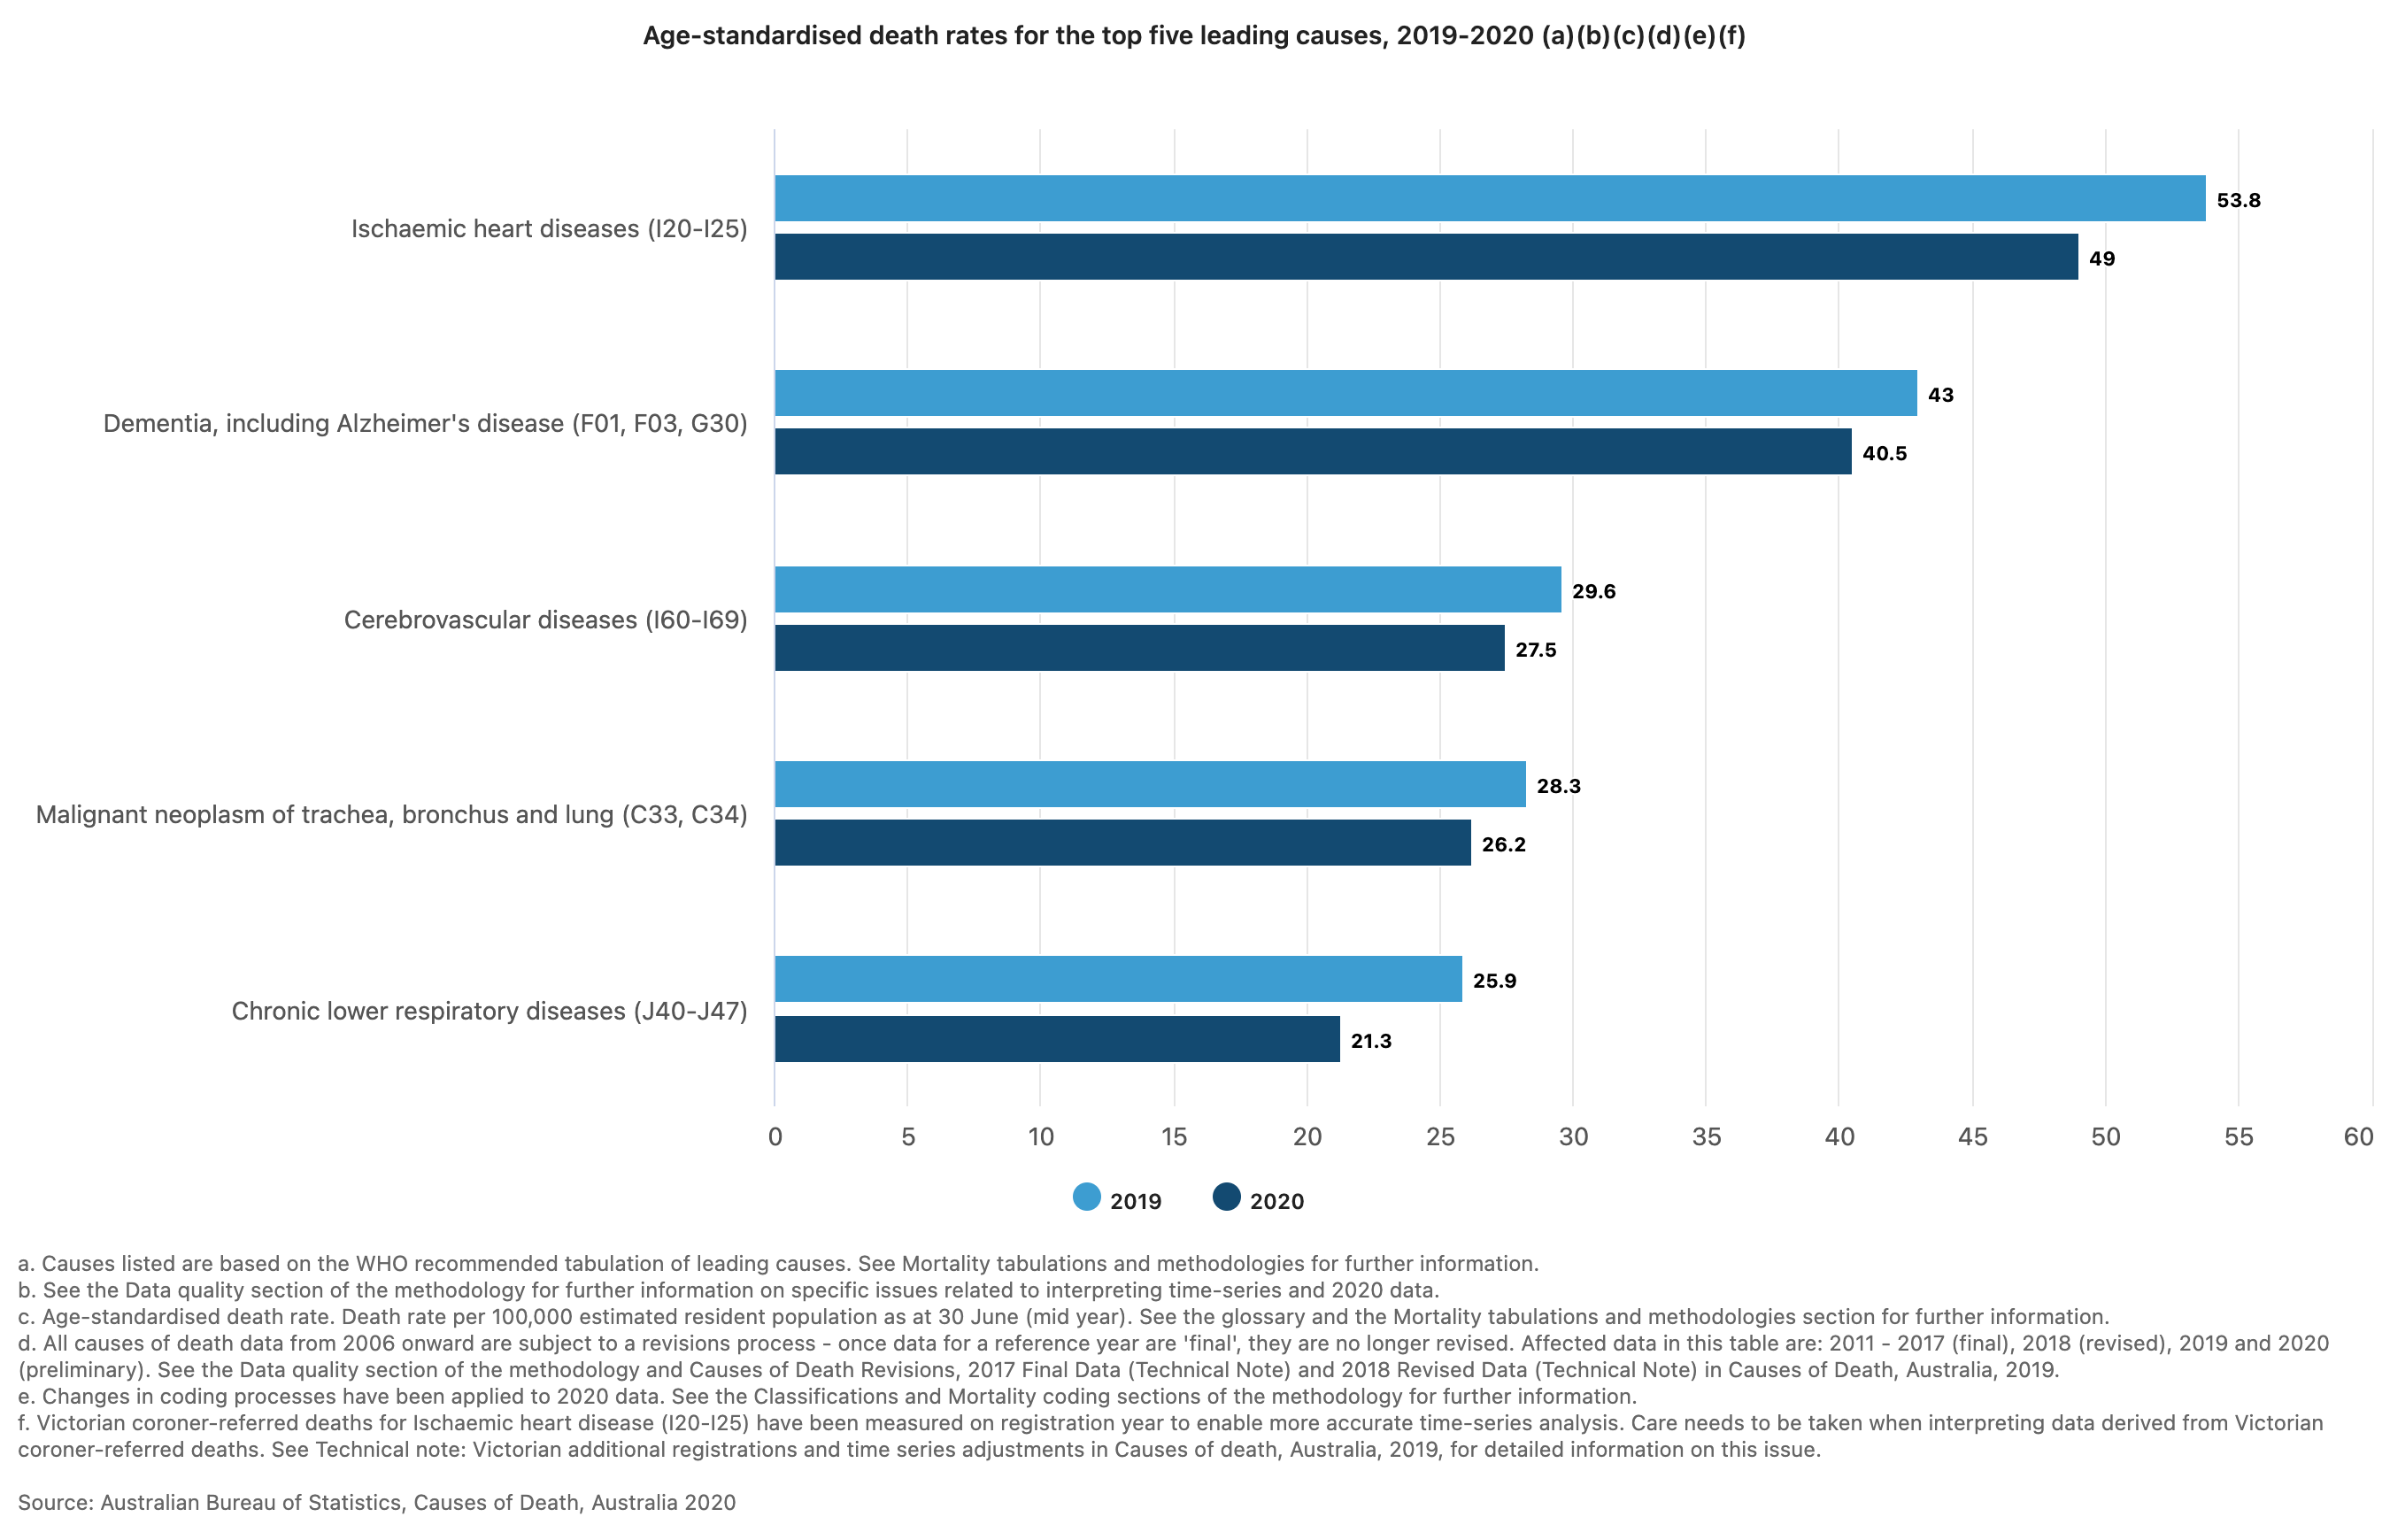
\includegraphics[width=1\linewidth]{img/mod01/cause-death}

\hypertarget{inferential-statistics}{%
\subsection{Inferential statistics}\label{inferential-statistics}}

Inferential statistics use data collected from a sample of the population, to make conclusions (inferences) about the whole population (that the sample was drawn from).

The following example is about a sample of prisoners, from the National Prisoner Health Data Collection (NPHDC). The NPHDC is the main source of national data about the health of prisoners in Australia. It gathers information over a 2-week period from prison entrants, dischargees, prisoners visiting the prison health clinic, and prisoners taking prescribed medication.

We have information about the population of prisoners, given as the number of prisoners in Australia's prisons from the ABS website: \footnote{\url{http://www.abs.gov.au/ausstats/abs@.nsf/Lookup/by\%20Subject/4517.0~2015~Main\%20Features~Prisoner\%20characteristics,\%20Australia~28}}

\begin{quote}
At 30 June 2015: There were 36,134 prisoners in Australian prisons, an increase of 7\% (2,345 prisoners) from 30 June 2014.
\end{quote}

Characteristics (sex, age group and Indigenous status) of the sample of prisoners from the NPHDC are given in the following table. We can use this information to make inferences about the whole population of prisoners that the sample was drawn from (The health of Australia's prisoners 2015).

\begin{figure}[H]
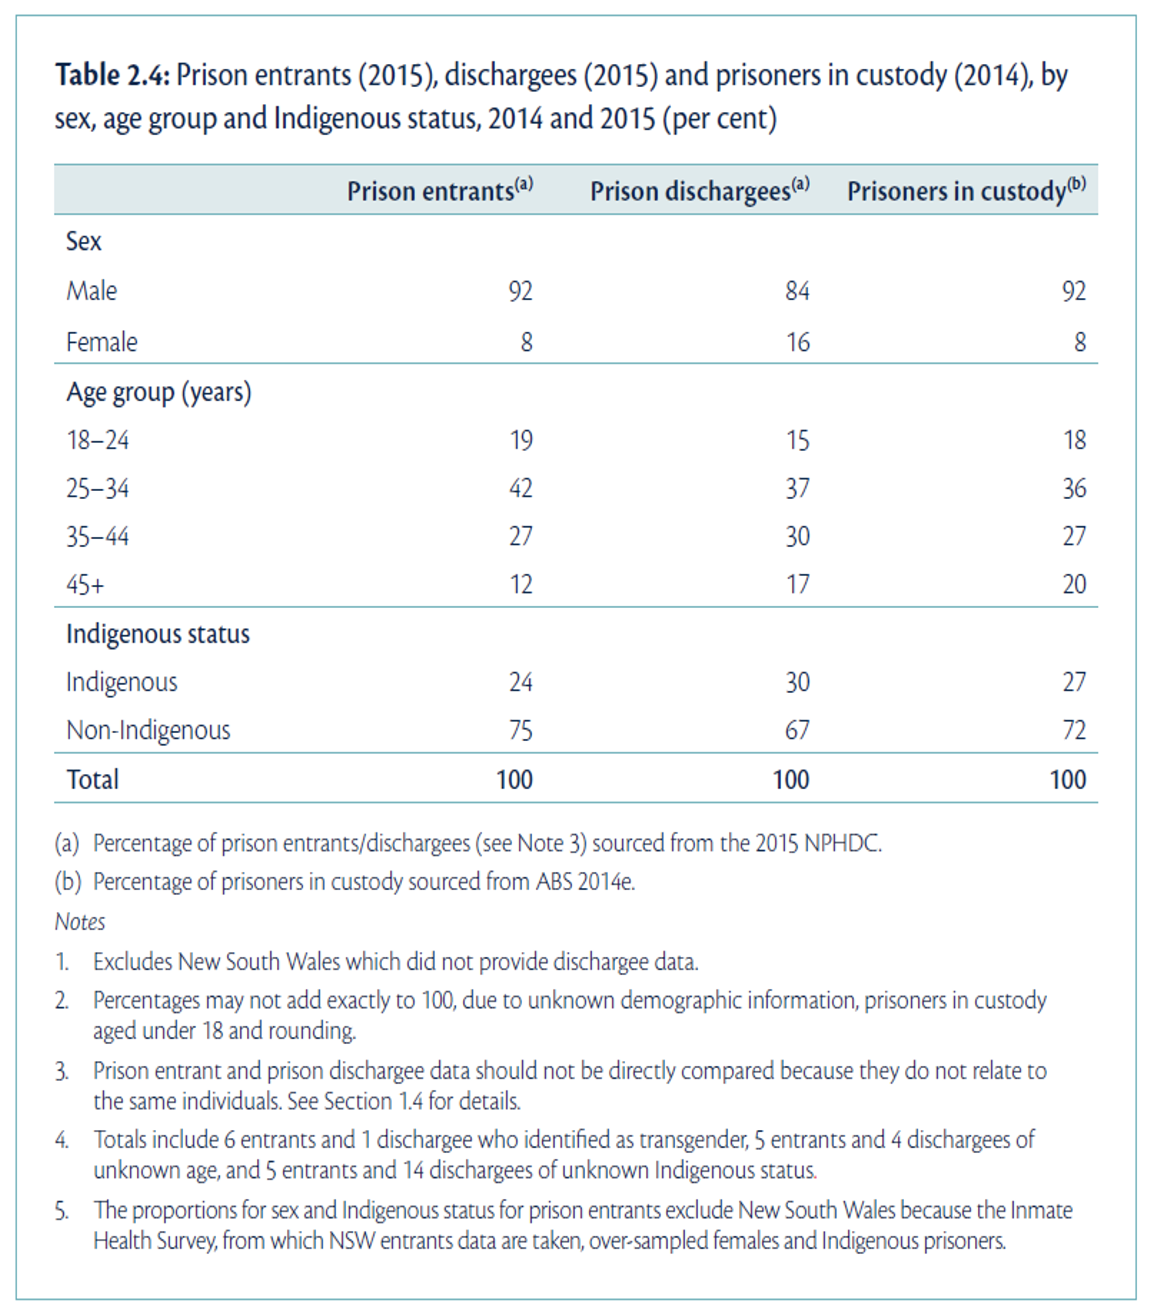
\includegraphics[width=0.66\linewidth]{img/mod01/prisoner-health} \caption{Characteristics of the sample of prisoners from the NPHDC}\label{fig:fig1-2}
\end{figure}

\hypertarget{variables}{%
\section{Variables}\label{variables}}

A variable is simply a characteristic that is being measured or observed. For example, height, weight, eye colour, income, country of birth are all types of variables.

When we are examining associations between variables, we may also use the terms: outcome variable (sometimes called a dependent variable) and explanatory variable (sometimes called an independent variable).

For example, some rural areas of Bangladesh have a very high concentration of arsenic in the drinking water. Children who consume arsenic-contaminated water become malnourished. In this example, being malnourished is the outcome variable which is being caused, or influenced, by the exposure variable: arsenic-contaminated water. Thus, the outcome variable is the variable of interest which may change in response to some exposure.

\hypertarget{types-of-data}{%
\subsection{Types of data}\label{types-of-data}}

Data are groups of information that represent the qualitative or quantitative attributes of variables or a group of variables. For example, the ages of students attending a university gym in a particular hour were recorded. The thirty ages are given below:

 
  \providecommand{\huxb}[2]{\arrayrulecolor[RGB]{#1}\global\arrayrulewidth=#2pt}
  \providecommand{\huxvb}[2]{\color[RGB]{#1}\vrule width #2pt}
  \providecommand{\huxtpad}[1]{\rule{0pt}{#1}}
  \providecommand{\huxbpad}[1]{\rule[-#1]{0pt}{#1}}

\begin{table}[ht]
\begin{centerbox}
\begin{threeparttable}
\captionsetup{justification=centering,singlelinecheck=off}
\caption{\label{tab:tab1-ages} Age of 30 gym attendees}
 \setlength{\tabcolsep}{0pt}
\begin{tabularx}{0.8\textwidth}{p{0.133333333333333\textwidth} p{0.133333333333333\textwidth} p{0.133333333333333\textwidth} p{0.133333333333333\textwidth} p{0.133333333333333\textwidth} p{0.133333333333333\textwidth}}


\hhline{>{\huxb{0, 0, 0}{0.4}}->{\huxb{0, 0, 0}{0.4}}->{\huxb{0, 0, 0}{0.4}}->{\huxb{0, 0, 0}{0.4}}->{\huxb{0, 0, 0}{0.4}}->{\huxb{0, 0, 0}{0.4}}-}
\arrayrulecolor{black}

\multicolumn{1}{!{\huxvb{0, 0, 0}{0}}p{0.133333333333333\textwidth}!{\huxvb{0, 0, 0}{0}}}{\hspace{0pt}\parbox[b]{0.133333333333333\textwidth-0pt-6pt}{\huxtpad{6pt + 1em}\raggedleft 18\huxbpad{6pt}}} &
\multicolumn{1}{p{0.133333333333333\textwidth}!{\huxvb{0, 0, 0}{0}}}{\hspace{6pt}\parbox[b]{0.133333333333333\textwidth-6pt-6pt}{\huxtpad{6pt + 1em}\raggedleft 17\huxbpad{6pt}}} &
\multicolumn{1}{p{0.133333333333333\textwidth}!{\huxvb{0, 0, 0}{0}}}{\hspace{6pt}\parbox[b]{0.133333333333333\textwidth-6pt-6pt}{\huxtpad{6pt + 1em}\raggedleft 20\huxbpad{6pt}}} &
\multicolumn{1}{p{0.133333333333333\textwidth}!{\huxvb{0, 0, 0}{0}}}{\hspace{6pt}\parbox[b]{0.133333333333333\textwidth-6pt-6pt}{\huxtpad{6pt + 1em}\raggedleft 21\huxbpad{6pt}}} &
\multicolumn{1}{p{0.133333333333333\textwidth}!{\huxvb{0, 0, 0}{0}}}{\hspace{6pt}\parbox[b]{0.133333333333333\textwidth-6pt-6pt}{\huxtpad{6pt + 1em}\raggedleft 23\huxbpad{6pt}}} &
\multicolumn{1}{p{0.133333333333333\textwidth}!{\huxvb{0, 0, 0}{0}}}{\hspace{6pt}\parbox[b]{0.133333333333333\textwidth-6pt-0pt}{\huxtpad{6pt + 1em}\raggedleft 19\huxbpad{6pt}}} \tabularnewline[-0.5pt]


\hhline{}
\arrayrulecolor{black}

\multicolumn{1}{!{\huxvb{0, 0, 0}{0}}p{0.133333333333333\textwidth}!{\huxvb{0, 0, 0}{0}}}{\hspace{0pt}\parbox[b]{0.133333333333333\textwidth-0pt-6pt}{\huxtpad{6pt + 1em}\raggedleft 19\huxbpad{6pt}}} &
\multicolumn{1}{p{0.133333333333333\textwidth}!{\huxvb{0, 0, 0}{0}}}{\hspace{6pt}\parbox[b]{0.133333333333333\textwidth-6pt-6pt}{\huxtpad{6pt + 1em}\raggedleft 18\huxbpad{6pt}}} &
\multicolumn{1}{p{0.133333333333333\textwidth}!{\huxvb{0, 0, 0}{0}}}{\hspace{6pt}\parbox[b]{0.133333333333333\textwidth-6pt-6pt}{\huxtpad{6pt + 1em}\raggedleft 18\huxbpad{6pt}}} &
\multicolumn{1}{p{0.133333333333333\textwidth}!{\huxvb{0, 0, 0}{0}}}{\hspace{6pt}\parbox[b]{0.133333333333333\textwidth-6pt-6pt}{\huxtpad{6pt + 1em}\raggedleft 20\huxbpad{6pt}}} &
\multicolumn{1}{p{0.133333333333333\textwidth}!{\huxvb{0, 0, 0}{0}}}{\hspace{6pt}\parbox[b]{0.133333333333333\textwidth-6pt-6pt}{\huxtpad{6pt + 1em}\raggedleft 21\huxbpad{6pt}}} &
\multicolumn{1}{p{0.133333333333333\textwidth}!{\huxvb{0, 0, 0}{0}}}{\hspace{6pt}\parbox[b]{0.133333333333333\textwidth-6pt-0pt}{\huxtpad{6pt + 1em}\raggedleft 23\huxbpad{6pt}}} \tabularnewline[-0.5pt]


\hhline{}
\arrayrulecolor{black}

\multicolumn{1}{!{\huxvb{0, 0, 0}{0}}p{0.133333333333333\textwidth}!{\huxvb{0, 0, 0}{0}}}{\hspace{0pt}\parbox[b]{0.133333333333333\textwidth-0pt-6pt}{\huxtpad{6pt + 1em}\raggedleft 20\huxbpad{6pt}}} &
\multicolumn{1}{p{0.133333333333333\textwidth}!{\huxvb{0, 0, 0}{0}}}{\hspace{6pt}\parbox[b]{0.133333333333333\textwidth-6pt-6pt}{\huxtpad{6pt + 1em}\raggedleft 23\huxbpad{6pt}}} &
\multicolumn{1}{p{0.133333333333333\textwidth}!{\huxvb{0, 0, 0}{0}}}{\hspace{6pt}\parbox[b]{0.133333333333333\textwidth-6pt-6pt}{\huxtpad{6pt + 1em}\raggedleft 19\huxbpad{6pt}}} &
\multicolumn{1}{p{0.133333333333333\textwidth}!{\huxvb{0, 0, 0}{0}}}{\hspace{6pt}\parbox[b]{0.133333333333333\textwidth-6pt-6pt}{\huxtpad{6pt + 1em}\raggedleft 21\huxbpad{6pt}}} &
\multicolumn{1}{p{0.133333333333333\textwidth}!{\huxvb{0, 0, 0}{0}}}{\hspace{6pt}\parbox[b]{0.133333333333333\textwidth-6pt-6pt}{\huxtpad{6pt + 1em}\raggedleft 19\huxbpad{6pt}}} &
\multicolumn{1}{p{0.133333333333333\textwidth}!{\huxvb{0, 0, 0}{0}}}{\hspace{6pt}\parbox[b]{0.133333333333333\textwidth-6pt-0pt}{\huxtpad{6pt + 1em}\raggedleft 20\huxbpad{6pt}}} \tabularnewline[-0.5pt]


\hhline{}
\arrayrulecolor{black}

\multicolumn{1}{!{\huxvb{0, 0, 0}{0}}p{0.133333333333333\textwidth}!{\huxvb{0, 0, 0}{0}}}{\hspace{0pt}\parbox[b]{0.133333333333333\textwidth-0pt-6pt}{\huxtpad{6pt + 1em}\raggedleft 20\huxbpad{6pt}}} &
\multicolumn{1}{p{0.133333333333333\textwidth}!{\huxvb{0, 0, 0}{0}}}{\hspace{6pt}\parbox[b]{0.133333333333333\textwidth-6pt-6pt}{\huxtpad{6pt + 1em}\raggedleft 22\huxbpad{6pt}}} &
\multicolumn{1}{p{0.133333333333333\textwidth}!{\huxvb{0, 0, 0}{0}}}{\hspace{6pt}\parbox[b]{0.133333333333333\textwidth-6pt-6pt}{\huxtpad{6pt + 1em}\raggedleft 19\huxbpad{6pt}}} &
\multicolumn{1}{p{0.133333333333333\textwidth}!{\huxvb{0, 0, 0}{0}}}{\hspace{6pt}\parbox[b]{0.133333333333333\textwidth-6pt-6pt}{\huxtpad{6pt + 1em}\raggedleft 22\huxbpad{6pt}}} &
\multicolumn{1}{p{0.133333333333333\textwidth}!{\huxvb{0, 0, 0}{0}}}{\hspace{6pt}\parbox[b]{0.133333333333333\textwidth-6pt-6pt}{\huxtpad{6pt + 1em}\raggedleft 20\huxbpad{6pt}}} &
\multicolumn{1}{p{0.133333333333333\textwidth}!{\huxvb{0, 0, 0}{0}}}{\hspace{6pt}\parbox[b]{0.133333333333333\textwidth-6pt-0pt}{\huxtpad{6pt + 1em}\raggedleft 21\huxbpad{6pt}}} \tabularnewline[-0.5pt]


\hhline{}
\arrayrulecolor{black}

\multicolumn{1}{!{\huxvb{0, 0, 0}{0}}p{0.133333333333333\textwidth}!{\huxvb{0, 0, 0}{0}}}{\hspace{0pt}\parbox[b]{0.133333333333333\textwidth-0pt-6pt}{\huxtpad{6pt + 1em}\raggedleft 18\huxbpad{6pt}}} &
\multicolumn{1}{p{0.133333333333333\textwidth}!{\huxvb{0, 0, 0}{0}}}{\hspace{6pt}\parbox[b]{0.133333333333333\textwidth-6pt-6pt}{\huxtpad{6pt + 1em}\raggedleft 23\huxbpad{6pt}}} &
\multicolumn{1}{p{0.133333333333333\textwidth}!{\huxvb{0, 0, 0}{0}}}{\hspace{6pt}\parbox[b]{0.133333333333333\textwidth-6pt-6pt}{\huxtpad{6pt + 1em}\raggedleft 24\huxbpad{6pt}}} &
\multicolumn{1}{p{0.133333333333333\textwidth}!{\huxvb{0, 0, 0}{0}}}{\hspace{6pt}\parbox[b]{0.133333333333333\textwidth-6pt-6pt}{\huxtpad{6pt + 1em}\raggedleft 18\huxbpad{6pt}}} &
\multicolumn{1}{p{0.133333333333333\textwidth}!{\huxvb{0, 0, 0}{0}}}{\hspace{6pt}\parbox[b]{0.133333333333333\textwidth-6pt-6pt}{\huxtpad{6pt + 1em}\raggedleft 20\huxbpad{6pt}}} &
\multicolumn{1}{p{0.133333333333333\textwidth}!{\huxvb{0, 0, 0}{0}}}{\hspace{6pt}\parbox[b]{0.133333333333333\textwidth-6pt-0pt}{\huxtpad{6pt + 1em}\raggedleft 21\huxbpad{6pt}}} \tabularnewline[-0.5pt]


\hhline{>{\huxb{0, 0, 0}{0.4}}->{\huxb{0, 0, 0}{0.4}}->{\huxb{0, 0, 0}{0.4}}->{\huxb{0, 0, 0}{0.4}}->{\huxb{0, 0, 0}{0.4}}->{\huxb{0, 0, 0}{0.4}}-}
\arrayrulecolor{black}
\end{tabularx}
\end{threeparttable}\par\end{centerbox}

\end{table}
 

The variable here is age and there are 30 observations recorded.

\textbf{Quantitative} data are numerical data that can be measured or counted such as age, weight, height, etc. These data can be discrete or continuous. Biostatistics mostly deals with quantitative variables or numerical data.

A \textbf{discrete} variable can have only one of a distinct set of values. For a discrete variable, observations are based on a count where both ordering and magnitude are important, such that numbers represent actual measurable quantities rather than mere labels.

For example, the number of cancer cases in a specified area emerging over a certain period, the number of motorbike accidents in Sydney, the number of times a woman has given birth, the number of beds in a hospital. It is noteworthy that natural ordering exists among the data points, that is, a hospital with 100 beds has more beds than a hospital with 75 beds. Moreover, a difference between 40 and 50 beds is the same as the difference between 80 and 90 beds. A discrete variable can take only non-negative integer values: a woman cannot have 5.7 births. However, we can calculate summaries of discrete variables that are not necessarily discrete. For instance, if one woman has given birth four times and another woman 5 times, then on average, these two women have 4.5 births.

\textbf{Continuous} data can take any values within a defined range.

For example, age, height, weight or blood pressure, are continuous variables because we can make any divisions we want on them, and they can be measured as small as the instrument allows. As an illustration, if two people have the same blood pressure measured to the nearest millimetre of mercury, we may get a difference between them if the blood pressure is measured to the nearest tenth of millimetre. If they are still the same (to the nearest tenth of a millimetre), we can measure them with even finer gradations until we can see a difference.

\textbf{Qualitative} data have values that describe a `quality' or `characteristic'. Categorical data are qualitative data and do not have measurable numeric values. These data can be nominal or ordinal.

A \textbf{nominal} variable consists of unordered categories. For example, gender, race, ethnic group, religion, eye colour etc. Both the order and magnitude of a nominal variable are unimportant. If a nominal variable takes on one of two distinct categories, such as black or white then it is called dichotomous or binary variable. Other examples would be male or female; smoker or non-smoker; exposed to arsenic or not exposed. A number is often used to represent (label) each of the categories; for example, males could be assigned the value 1 and females 0; in the case of exposed and unexposed, exposed could be assigned 1 and unexposed 0. A nominal variable can also have more than two categories, such as blood group, with labels and categories as follows (1=Group A, 2=Group B, 3=Group AB, 4=Group O). Numbers are used for the sake of convenience of analysis when using a computer package.

\textbf{Ordinal} data consist of ordered categories where differences between categories are important, such as socioeconomic status (low, medium, high) or student evaluation rating could be classified according to their level of satisfaction, where 1 represents excellent, 2 is satisfactory and 3 is unsatisfactory. Here natural order exists among the categories, where a smaller number represents higher satisfaction.

\hypertarget{presenting-data}{%
\section{Presenting data}\label{presenting-data}}

We will now look at ways to present frequency information numerically in tables and graphs.

\hypertarget{frequency-tables}{%
\subsection{Frequency tables}\label{frequency-tables}}

\hypertarget{worked-example}{%
\subsubsection{Worked example}\label{worked-example}}

Consider the ages of 30 students visiting a university gym in a particular hour presented in Table \ref{tab:tab1-ages}. This information is difficult to interpret in its raw form, but becomes more clear if the ages are grouped in a frequency table as shown in Table \ref{tab:tab1-ages-freq1}.

 
  \providecommand{\huxb}[2]{\arrayrulecolor[RGB]{#1}\global\arrayrulewidth=#2pt}
  \providecommand{\huxvb}[2]{\color[RGB]{#1}\vrule width #2pt}
  \providecommand{\huxtpad}[1]{\rule{0pt}{#1}}
  \providecommand{\huxbpad}[1]{\rule[-#1]{0pt}{#1}}

\begin{table}[ht]
\begin{centerbox}
\begin{threeparttable}
\captionsetup{justification=centering,singlelinecheck=off}
\caption{\label{tab:tab1-ages-freq1} Frequency of ages of students visiting a gym}
 \setlength{\tabcolsep}{0pt}
\begin{tabularx}{0.6\textwidth}{p{0.3\textwidth} p{0.3\textwidth}}


\hhline{>{\huxb{0, 0, 0}{0.4}}->{\huxb{0, 0, 0}{0.4}}-}
\arrayrulecolor{black}

\multicolumn{1}{!{\huxvb{0, 0, 0}{0}}p{0.3\textwidth}!{\huxvb{0, 0, 0}{0}}}{\hspace{0pt}\parbox[b]{0.3\textwidth-0pt-6pt}{\huxtpad{6pt + 1em}\raggedleft \textbf{Age}\huxbpad{6pt}}} &
\multicolumn{1}{p{0.3\textwidth}!{\huxvb{0, 0, 0}{0}}}{\hspace{6pt}\parbox[b]{0.3\textwidth-6pt-0pt}{\huxtpad{6pt + 1em}\raggedleft \textbf{Frequency}\huxbpad{6pt}}} \tabularnewline[-0.5pt]


\hhline{>{\huxb{0, 0, 0}{0.4}}->{\huxb{0, 0, 0}{0.4}}-}
\arrayrulecolor{black}

\multicolumn{1}{!{\huxvb{0, 0, 0}{0}}p{0.3\textwidth}!{\huxvb{0, 0, 0}{0}}}{\hspace{0pt}\parbox[b]{0.3\textwidth-0pt-6pt}{\huxtpad{6pt + 1em}\raggedleft 17\huxbpad{6pt}}} &
\multicolumn{1}{p{0.3\textwidth}!{\huxvb{0, 0, 0}{0}}}{\hspace{6pt}\parbox[b]{0.3\textwidth-6pt-0pt}{\huxtpad{6pt + 1em}\raggedleft 1\huxbpad{6pt}}} \tabularnewline[-0.5pt]


\hhline{}
\arrayrulecolor{black}

\multicolumn{1}{!{\huxvb{0, 0, 0}{0}}p{0.3\textwidth}!{\huxvb{0, 0, 0}{0}}}{\hspace{0pt}\parbox[b]{0.3\textwidth-0pt-6pt}{\huxtpad{6pt + 1em}\raggedleft 18\huxbpad{6pt}}} &
\multicolumn{1}{p{0.3\textwidth}!{\huxvb{0, 0, 0}{0}}}{\hspace{6pt}\parbox[b]{0.3\textwidth-6pt-0pt}{\huxtpad{6pt + 1em}\raggedleft 5\huxbpad{6pt}}} \tabularnewline[-0.5pt]


\hhline{}
\arrayrulecolor{black}

\multicolumn{1}{!{\huxvb{0, 0, 0}{0}}p{0.3\textwidth}!{\huxvb{0, 0, 0}{0}}}{\hspace{0pt}\parbox[b]{0.3\textwidth-0pt-6pt}{\huxtpad{6pt + 1em}\raggedleft 19\huxbpad{6pt}}} &
\multicolumn{1}{p{0.3\textwidth}!{\huxvb{0, 0, 0}{0}}}{\hspace{6pt}\parbox[b]{0.3\textwidth-6pt-0pt}{\huxtpad{6pt + 1em}\raggedleft 5\huxbpad{6pt}}} \tabularnewline[-0.5pt]


\hhline{}
\arrayrulecolor{black}

\multicolumn{1}{!{\huxvb{0, 0, 0}{0}}p{0.3\textwidth}!{\huxvb{0, 0, 0}{0}}}{\hspace{0pt}\parbox[b]{0.3\textwidth-0pt-6pt}{\huxtpad{6pt + 1em}\raggedleft 20\huxbpad{6pt}}} &
\multicolumn{1}{p{0.3\textwidth}!{\huxvb{0, 0, 0}{0}}}{\hspace{6pt}\parbox[b]{0.3\textwidth-6pt-0pt}{\huxtpad{6pt + 1em}\raggedleft 7\huxbpad{6pt}}} \tabularnewline[-0.5pt]


\hhline{}
\arrayrulecolor{black}

\multicolumn{1}{!{\huxvb{0, 0, 0}{0}}p{0.3\textwidth}!{\huxvb{0, 0, 0}{0}}}{\hspace{0pt}\parbox[b]{0.3\textwidth-0pt-6pt}{\huxtpad{6pt + 1em}\raggedleft 21\huxbpad{6pt}}} &
\multicolumn{1}{p{0.3\textwidth}!{\huxvb{0, 0, 0}{0}}}{\hspace{6pt}\parbox[b]{0.3\textwidth-6pt-0pt}{\huxtpad{6pt + 1em}\raggedleft 5\huxbpad{6pt}}} \tabularnewline[-0.5pt]


\hhline{}
\arrayrulecolor{black}

\multicolumn{1}{!{\huxvb{0, 0, 0}{0}}p{0.3\textwidth}!{\huxvb{0, 0, 0}{0}}}{\hspace{0pt}\parbox[b]{0.3\textwidth-0pt-6pt}{\huxtpad{6pt + 1em}\raggedleft 22\huxbpad{6pt}}} &
\multicolumn{1}{p{0.3\textwidth}!{\huxvb{0, 0, 0}{0}}}{\hspace{6pt}\parbox[b]{0.3\textwidth-6pt-0pt}{\huxtpad{6pt + 1em}\raggedleft 2\huxbpad{6pt}}} \tabularnewline[-0.5pt]


\hhline{}
\arrayrulecolor{black}

\multicolumn{1}{!{\huxvb{0, 0, 0}{0}}p{0.3\textwidth}!{\huxvb{0, 0, 0}{0}}}{\hspace{0pt}\parbox[b]{0.3\textwidth-0pt-6pt}{\huxtpad{6pt + 1em}\raggedleft 23\huxbpad{6pt}}} &
\multicolumn{1}{p{0.3\textwidth}!{\huxvb{0, 0, 0}{0}}}{\hspace{6pt}\parbox[b]{0.3\textwidth-6pt-0pt}{\huxtpad{6pt + 1em}\raggedleft 4\huxbpad{6pt}}} \tabularnewline[-0.5pt]


\hhline{}
\arrayrulecolor{black}

\multicolumn{1}{!{\huxvb{0, 0, 0}{0}}p{0.3\textwidth}!{\huxvb{0, 0, 0}{0}}}{\hspace{0pt}\parbox[b]{0.3\textwidth-0pt-6pt}{\huxtpad{6pt + 1em}\raggedleft 24\huxbpad{6pt}}} &
\multicolumn{1}{p{0.3\textwidth}!{\huxvb{0, 0, 0}{0}}}{\hspace{6pt}\parbox[b]{0.3\textwidth-6pt-0pt}{\huxtpad{6pt + 1em}\raggedleft 1\huxbpad{6pt}}} \tabularnewline[-0.5pt]


\hhline{}
\arrayrulecolor{black}

\multicolumn{1}{!{\huxvb{0, 0, 0}{0}}p{0.3\textwidth}!{\huxvb{0, 0, 0}{0}}}{\hspace{0pt}\parbox[b]{0.3\textwidth-0pt-6pt}{\huxtpad{6pt + 1em}\raggedleft Total\huxbpad{6pt}}} &
\multicolumn{1}{p{0.3\textwidth}!{\huxvb{0, 0, 0}{0}}}{\hspace{6pt}\parbox[b]{0.3\textwidth-6pt-0pt}{\huxtpad{6pt + 1em}\raggedleft 30\huxbpad{6pt}}} \tabularnewline[-0.5pt]


\hhline{>{\huxb{0, 0, 0}{0.4}}->{\huxb{0, 0, 0}{0.4}}-}
\arrayrulecolor{black}
\end{tabularx}
\end{threeparttable}\par\end{centerbox}

\end{table}
 

The frequency is a count of the number of individuals of each age in the corresponding row. Three more columns can be added to the frequency table to give further insight: relative frequency, cumulative frequency and cumulative relative frequency (Table \ref{tab:tab1-ages-freq2}).

 
  \providecommand{\huxb}[2]{\arrayrulecolor[RGB]{#1}\global\arrayrulewidth=#2pt}
  \providecommand{\huxvb}[2]{\color[RGB]{#1}\vrule width #2pt}
  \providecommand{\huxtpad}[1]{\rule{0pt}{#1}}
  \providecommand{\huxbpad}[1]{\rule[-#1]{0pt}{#1}}

\begin{table}[ht]
\begin{centerbox}
\begin{threeparttable}
\captionsetup{justification=centering,singlelinecheck=off}
\caption{\label{tab:tab1-ages-freq2} Frequency of ages of students visiting a gym}
 \setlength{\tabcolsep}{0pt}
\begin{tabularx}{0.9\textwidth}{p{0.18\textwidth} p{0.18\textwidth} p{0.18\textwidth} p{0.18\textwidth} p{0.18\textwidth}}


\hhline{>{\huxb{0, 0, 0}{0.4}}->{\huxb{0, 0, 0}{0.4}}->{\huxb{0, 0, 0}{0.4}}->{\huxb{0, 0, 0}{0.4}}->{\huxb{0, 0, 0}{0.4}}-}
\arrayrulecolor{black}

\multicolumn{1}{!{\huxvb{0, 0, 0}{0}}p{0.18\textwidth}!{\huxvb{0, 0, 0}{0}}}{\hspace{0pt}\parbox[b]{0.18\textwidth-0pt-6pt}{\huxtpad{6pt + 1em}\raggedleft \textbf{Age}\huxbpad{6pt}}} &
\multicolumn{1}{p{0.18\textwidth}!{\huxvb{0, 0, 0}{0}}}{\hspace{6pt}\parbox[b]{0.18\textwidth-6pt-6pt}{\huxtpad{6pt + 1em}\raggedleft \textbf{Frequency}\huxbpad{6pt}}} &
\multicolumn{1}{p{0.18\textwidth}!{\huxvb{0, 0, 0}{0}}}{\hspace{6pt}\parbox[b]{0.18\textwidth-6pt-6pt}{\huxtpad{6pt + 1em}\raggedleft \textbf{Relative frequency (\%)}\huxbpad{6pt}}} &
\multicolumn{1}{p{0.18\textwidth}!{\huxvb{0, 0, 0}{0}}}{\hspace{6pt}\parbox[b]{0.18\textwidth-6pt-6pt}{\huxtpad{6pt + 1em}\raggedleft \textbf{Cumulative frequency}\huxbpad{6pt}}} &
\multicolumn{1}{p{0.18\textwidth}!{\huxvb{0, 0, 0}{0}}}{\hspace{6pt}\parbox[b]{0.18\textwidth-6pt-0pt}{\huxtpad{6pt + 1em}\raggedleft \textbf{Cumulative relative frequency (\%)}\huxbpad{6pt}}} \tabularnewline[-0.5pt]


\hhline{>{\huxb{0, 0, 0}{0.4}}->{\huxb{0, 0, 0}{0.4}}->{\huxb{0, 0, 0}{0.4}}->{\huxb{0, 0, 0}{0.4}}->{\huxb{0, 0, 0}{0.4}}-}
\arrayrulecolor{black}

\multicolumn{1}{!{\huxvb{0, 0, 0}{0}}p{0.18\textwidth}!{\huxvb{0, 0, 0}{0}}}{\hspace{0pt}\parbox[b]{0.18\textwidth-0pt-6pt}{\huxtpad{6pt + 1em}\raggedleft 17\huxbpad{6pt}}} &
\multicolumn{1}{p{0.18\textwidth}!{\huxvb{0, 0, 0}{0}}}{\hspace{6pt}\parbox[b]{0.18\textwidth-6pt-6pt}{\huxtpad{6pt + 1em}\raggedleft 1\huxbpad{6pt}}} &
\multicolumn{1}{p{0.18\textwidth}!{\huxvb{0, 0, 0}{0}}}{\hspace{6pt}\parbox[b]{0.18\textwidth-6pt-6pt}{\huxtpad{6pt + 1em}\raggedleft 3\huxbpad{6pt}}} &
\multicolumn{1}{p{0.18\textwidth}!{\huxvb{0, 0, 0}{0}}}{\hspace{6pt}\parbox[b]{0.18\textwidth-6pt-6pt}{\huxtpad{6pt + 1em}\raggedleft 1\huxbpad{6pt}}} &
\multicolumn{1}{p{0.18\textwidth}!{\huxvb{0, 0, 0}{0}}}{\hspace{6pt}\parbox[b]{0.18\textwidth-6pt-0pt}{\huxtpad{6pt + 1em}\raggedleft 3\huxbpad{6pt}}} \tabularnewline[-0.5pt]


\hhline{}
\arrayrulecolor{black}

\multicolumn{1}{!{\huxvb{0, 0, 0}{0}}p{0.18\textwidth}!{\huxvb{0, 0, 0}{0}}}{\hspace{0pt}\parbox[b]{0.18\textwidth-0pt-6pt}{\huxtpad{6pt + 1em}\raggedleft 18\huxbpad{6pt}}} &
\multicolumn{1}{p{0.18\textwidth}!{\huxvb{0, 0, 0}{0}}}{\hspace{6pt}\parbox[b]{0.18\textwidth-6pt-6pt}{\huxtpad{6pt + 1em}\raggedleft 5\huxbpad{6pt}}} &
\multicolumn{1}{p{0.18\textwidth}!{\huxvb{0, 0, 0}{0}}}{\hspace{6pt}\parbox[b]{0.18\textwidth-6pt-6pt}{\huxtpad{6pt + 1em}\raggedleft 17\huxbpad{6pt}}} &
\multicolumn{1}{p{0.18\textwidth}!{\huxvb{0, 0, 0}{0}}}{\hspace{6pt}\parbox[b]{0.18\textwidth-6pt-6pt}{\huxtpad{6pt + 1em}\raggedleft 6\huxbpad{6pt}}} &
\multicolumn{1}{p{0.18\textwidth}!{\huxvb{0, 0, 0}{0}}}{\hspace{6pt}\parbox[b]{0.18\textwidth-6pt-0pt}{\huxtpad{6pt + 1em}\raggedleft 20\huxbpad{6pt}}} \tabularnewline[-0.5pt]


\hhline{}
\arrayrulecolor{black}

\multicolumn{1}{!{\huxvb{0, 0, 0}{0}}p{0.18\textwidth}!{\huxvb{0, 0, 0}{0}}}{\hspace{0pt}\parbox[b]{0.18\textwidth-0pt-6pt}{\huxtpad{6pt + 1em}\raggedleft 19\huxbpad{6pt}}} &
\multicolumn{1}{p{0.18\textwidth}!{\huxvb{0, 0, 0}{0}}}{\hspace{6pt}\parbox[b]{0.18\textwidth-6pt-6pt}{\huxtpad{6pt + 1em}\raggedleft 5\huxbpad{6pt}}} &
\multicolumn{1}{p{0.18\textwidth}!{\huxvb{0, 0, 0}{0}}}{\hspace{6pt}\parbox[b]{0.18\textwidth-6pt-6pt}{\huxtpad{6pt + 1em}\raggedleft 17\huxbpad{6pt}}} &
\multicolumn{1}{p{0.18\textwidth}!{\huxvb{0, 0, 0}{0}}}{\hspace{6pt}\parbox[b]{0.18\textwidth-6pt-6pt}{\huxtpad{6pt + 1em}\raggedleft 11\huxbpad{6pt}}} &
\multicolumn{1}{p{0.18\textwidth}!{\huxvb{0, 0, 0}{0}}}{\hspace{6pt}\parbox[b]{0.18\textwidth-6pt-0pt}{\huxtpad{6pt + 1em}\raggedleft 37\huxbpad{6pt}}} \tabularnewline[-0.5pt]


\hhline{}
\arrayrulecolor{black}

\multicolumn{1}{!{\huxvb{0, 0, 0}{0}}p{0.18\textwidth}!{\huxvb{0, 0, 0}{0}}}{\hspace{0pt}\parbox[b]{0.18\textwidth-0pt-6pt}{\huxtpad{6pt + 1em}\raggedleft 20\huxbpad{6pt}}} &
\multicolumn{1}{p{0.18\textwidth}!{\huxvb{0, 0, 0}{0}}}{\hspace{6pt}\parbox[b]{0.18\textwidth-6pt-6pt}{\huxtpad{6pt + 1em}\raggedleft 7\huxbpad{6pt}}} &
\multicolumn{1}{p{0.18\textwidth}!{\huxvb{0, 0, 0}{0}}}{\hspace{6pt}\parbox[b]{0.18\textwidth-6pt-6pt}{\huxtpad{6pt + 1em}\raggedleft 23\huxbpad{6pt}}} &
\multicolumn{1}{p{0.18\textwidth}!{\huxvb{0, 0, 0}{0}}}{\hspace{6pt}\parbox[b]{0.18\textwidth-6pt-6pt}{\huxtpad{6pt + 1em}\raggedleft 18\huxbpad{6pt}}} &
\multicolumn{1}{p{0.18\textwidth}!{\huxvb{0, 0, 0}{0}}}{\hspace{6pt}\parbox[b]{0.18\textwidth-6pt-0pt}{\huxtpad{6pt + 1em}\raggedleft 60\huxbpad{6pt}}} \tabularnewline[-0.5pt]


\hhline{}
\arrayrulecolor{black}

\multicolumn{1}{!{\huxvb{0, 0, 0}{0}}p{0.18\textwidth}!{\huxvb{0, 0, 0}{0}}}{\hspace{0pt}\parbox[b]{0.18\textwidth-0pt-6pt}{\huxtpad{6pt + 1em}\raggedleft 21\huxbpad{6pt}}} &
\multicolumn{1}{p{0.18\textwidth}!{\huxvb{0, 0, 0}{0}}}{\hspace{6pt}\parbox[b]{0.18\textwidth-6pt-6pt}{\huxtpad{6pt + 1em}\raggedleft 5\huxbpad{6pt}}} &
\multicolumn{1}{p{0.18\textwidth}!{\huxvb{0, 0, 0}{0}}}{\hspace{6pt}\parbox[b]{0.18\textwidth-6pt-6pt}{\huxtpad{6pt + 1em}\raggedleft 17\huxbpad{6pt}}} &
\multicolumn{1}{p{0.18\textwidth}!{\huxvb{0, 0, 0}{0}}}{\hspace{6pt}\parbox[b]{0.18\textwidth-6pt-6pt}{\huxtpad{6pt + 1em}\raggedleft 23\huxbpad{6pt}}} &
\multicolumn{1}{p{0.18\textwidth}!{\huxvb{0, 0, 0}{0}}}{\hspace{6pt}\parbox[b]{0.18\textwidth-6pt-0pt}{\huxtpad{6pt + 1em}\raggedleft 77\huxbpad{6pt}}} \tabularnewline[-0.5pt]


\hhline{}
\arrayrulecolor{black}

\multicolumn{1}{!{\huxvb{0, 0, 0}{0}}p{0.18\textwidth}!{\huxvb{0, 0, 0}{0}}}{\hspace{0pt}\parbox[b]{0.18\textwidth-0pt-6pt}{\huxtpad{6pt + 1em}\raggedleft 22\huxbpad{6pt}}} &
\multicolumn{1}{p{0.18\textwidth}!{\huxvb{0, 0, 0}{0}}}{\hspace{6pt}\parbox[b]{0.18\textwidth-6pt-6pt}{\huxtpad{6pt + 1em}\raggedleft 2\huxbpad{6pt}}} &
\multicolumn{1}{p{0.18\textwidth}!{\huxvb{0, 0, 0}{0}}}{\hspace{6pt}\parbox[b]{0.18\textwidth-6pt-6pt}{\huxtpad{6pt + 1em}\raggedleft 7\huxbpad{6pt}}} &
\multicolumn{1}{p{0.18\textwidth}!{\huxvb{0, 0, 0}{0}}}{\hspace{6pt}\parbox[b]{0.18\textwidth-6pt-6pt}{\huxtpad{6pt + 1em}\raggedleft 25\huxbpad{6pt}}} &
\multicolumn{1}{p{0.18\textwidth}!{\huxvb{0, 0, 0}{0}}}{\hspace{6pt}\parbox[b]{0.18\textwidth-6pt-0pt}{\huxtpad{6pt + 1em}\raggedleft 83\huxbpad{6pt}}} \tabularnewline[-0.5pt]


\hhline{}
\arrayrulecolor{black}

\multicolumn{1}{!{\huxvb{0, 0, 0}{0}}p{0.18\textwidth}!{\huxvb{0, 0, 0}{0}}}{\hspace{0pt}\parbox[b]{0.18\textwidth-0pt-6pt}{\huxtpad{6pt + 1em}\raggedleft 23\huxbpad{6pt}}} &
\multicolumn{1}{p{0.18\textwidth}!{\huxvb{0, 0, 0}{0}}}{\hspace{6pt}\parbox[b]{0.18\textwidth-6pt-6pt}{\huxtpad{6pt + 1em}\raggedleft 4\huxbpad{6pt}}} &
\multicolumn{1}{p{0.18\textwidth}!{\huxvb{0, 0, 0}{0}}}{\hspace{6pt}\parbox[b]{0.18\textwidth-6pt-6pt}{\huxtpad{6pt + 1em}\raggedleft 13\huxbpad{6pt}}} &
\multicolumn{1}{p{0.18\textwidth}!{\huxvb{0, 0, 0}{0}}}{\hspace{6pt}\parbox[b]{0.18\textwidth-6pt-6pt}{\huxtpad{6pt + 1em}\raggedleft 29\huxbpad{6pt}}} &
\multicolumn{1}{p{0.18\textwidth}!{\huxvb{0, 0, 0}{0}}}{\hspace{6pt}\parbox[b]{0.18\textwidth-6pt-0pt}{\huxtpad{6pt + 1em}\raggedleft 97\huxbpad{6pt}}} \tabularnewline[-0.5pt]


\hhline{}
\arrayrulecolor{black}

\multicolumn{1}{!{\huxvb{0, 0, 0}{0}}p{0.18\textwidth}!{\huxvb{0, 0, 0}{0}}}{\hspace{0pt}\parbox[b]{0.18\textwidth-0pt-6pt}{\huxtpad{6pt + 1em}\raggedleft 24\huxbpad{6pt}}} &
\multicolumn{1}{p{0.18\textwidth}!{\huxvb{0, 0, 0}{0}}}{\hspace{6pt}\parbox[b]{0.18\textwidth-6pt-6pt}{\huxtpad{6pt + 1em}\raggedleft 1\huxbpad{6pt}}} &
\multicolumn{1}{p{0.18\textwidth}!{\huxvb{0, 0, 0}{0}}}{\hspace{6pt}\parbox[b]{0.18\textwidth-6pt-6pt}{\huxtpad{6pt + 1em}\raggedleft 3\huxbpad{6pt}}} &
\multicolumn{1}{p{0.18\textwidth}!{\huxvb{0, 0, 0}{0}}}{\hspace{6pt}\parbox[b]{0.18\textwidth-6pt-6pt}{\huxtpad{6pt + 1em}\raggedleft 30\huxbpad{6pt}}} &
\multicolumn{1}{p{0.18\textwidth}!{\huxvb{0, 0, 0}{0}}}{\hspace{6pt}\parbox[b]{0.18\textwidth-6pt-0pt}{\huxtpad{6pt + 1em}\raggedleft 100\huxbpad{6pt}}} \tabularnewline[-0.5pt]


\hhline{}
\arrayrulecolor{black}

\multicolumn{1}{!{\huxvb{0, 0, 0}{0}}p{0.18\textwidth}!{\huxvb{0, 0, 0}{0}}}{\hspace{0pt}\parbox[b]{0.18\textwidth-0pt-6pt}{\huxtpad{6pt + 1em}\raggedleft Total\huxbpad{6pt}}} &
\multicolumn{1}{p{0.18\textwidth}!{\huxvb{0, 0, 0}{0}}}{\hspace{6pt}\parbox[b]{0.18\textwidth-6pt-6pt}{\huxtpad{6pt + 1em}\raggedleft 30\huxbpad{6pt}}} &
\multicolumn{1}{p{0.18\textwidth}!{\huxvb{0, 0, 0}{0}}}{\hspace{6pt}\parbox[b]{0.18\textwidth-6pt-6pt}{\huxtpad{6pt + 1em}\raggedleft 100\huxbpad{6pt}}} &
\multicolumn{1}{p{0.18\textwidth}!{\huxvb{0, 0, 0}{0}}}{\hspace{6pt}\parbox[b]{0.18\textwidth-6pt-6pt}{\huxtpad{6pt + 1em}\raggedleft \huxbpad{6pt}}} &
\multicolumn{1}{p{0.18\textwidth}!{\huxvb{0, 0, 0}{0}}}{\hspace{6pt}\parbox[b]{0.18\textwidth-6pt-0pt}{\huxtpad{6pt + 1em}\raggedleft \huxbpad{6pt}}} \tabularnewline[-0.5pt]


\hhline{>{\huxb{0, 0, 0}{0.4}}->{\huxb{0, 0, 0}{0.4}}->{\huxb{0, 0, 0}{0.4}}->{\huxb{0, 0, 0}{0.4}}->{\huxb{0, 0, 0}{0.4}}-}
\arrayrulecolor{black}
\end{tabularx}
\end{threeparttable}\par\end{centerbox}

\end{table}
 

The relative frequency is the frequency expressed as a proportion or percentage of the total frequency. For example, 5 out of 30 students are aged 21, so the relative frequency is (5/30) \(\times\) 100 = 16.7\%.

The cumulative frequency here shows the total number of students less than or equal to a certain age, while the cumulative relative frequency is the percentage (of the total) who are less than a certain age. For example, the cumulative frequency of students at the gym aged 19 years or less is 1 + 5 + 5 = 11, and the cumulative relative frequency is (11/30) \(\times\) 100 = 36.7\%.

The information presented in Table \ref{tab:tab1-ages-freq2} is called the frequency distribution of the variable age. Frequency distributions can also be presented for qualitative (categorical) data.

For example, if we know that there are 12 males and 18 females in our data, this can be presented as in Table 1.4. We should not interpret the cumulative frequency for nominal data (e.g.~gender, eye colour or cancer types) as these data cannot be ranked. However, we can calculate the cumulative frequency for ordinal data (e.g.~student satisfaction level, cancer stage).

 
  \providecommand{\huxb}[2]{\arrayrulecolor[RGB]{#1}\global\arrayrulewidth=#2pt}
  \providecommand{\huxvb}[2]{\color[RGB]{#1}\vrule width #2pt}
  \providecommand{\huxtpad}[1]{\rule{0pt}{#1}}
  \providecommand{\huxbpad}[1]{\rule[-#1]{0pt}{#1}}

\begin{table}[ht]
\begin{centerbox}
\begin{threeparttable}
\captionsetup{justification=centering,singlelinecheck=off}
\caption{\label{tab:tab1-sex-freq} Frequency of sex of students visiting a gym}
 \setlength{\tabcolsep}{0pt}
\begin{tabularx}{0.9\textwidth}{p{0.3\textwidth} p{0.3\textwidth} p{0.3\textwidth}}


\hhline{>{\huxb{0, 0, 0}{0.4}}->{\huxb{0, 0, 0}{0.4}}->{\huxb{0, 0, 0}{0.4}}-}
\arrayrulecolor{black}

\multicolumn{1}{!{\huxvb{0, 0, 0}{0}}p{0.3\textwidth}!{\huxvb{0, 0, 0}{0}}}{\hspace{0pt}\parbox[b]{0.3\textwidth-0pt-6pt}{\huxtpad{6pt + 1em}\raggedleft \textbf{Sex}\huxbpad{6pt}}} &
\multicolumn{1}{p{0.3\textwidth}!{\huxvb{0, 0, 0}{0}}}{\hspace{6pt}\parbox[b]{0.3\textwidth-6pt-6pt}{\huxtpad{6pt + 1em}\raggedleft \textbf{Frequency}\huxbpad{6pt}}} &
\multicolumn{1}{p{0.3\textwidth}!{\huxvb{0, 0, 0}{0}}}{\hspace{6pt}\parbox[b]{0.3\textwidth-6pt-0pt}{\huxtpad{6pt + 1em}\raggedleft \textbf{Relative frequency (\%)}\huxbpad{6pt}}} \tabularnewline[-0.5pt]


\hhline{>{\huxb{0, 0, 0}{0.4}}->{\huxb{0, 0, 0}{0.4}}->{\huxb{0, 0, 0}{0.4}}-}
\arrayrulecolor{black}

\multicolumn{1}{!{\huxvb{0, 0, 0}{0}}p{0.3\textwidth}!{\huxvb{0, 0, 0}{0}}}{\hspace{0pt}\parbox[b]{0.3\textwidth-0pt-6pt}{\huxtpad{6pt + 1em}\raggedleft Male\huxbpad{6pt}}} &
\multicolumn{1}{p{0.3\textwidth}!{\huxvb{0, 0, 0}{0}}}{\hspace{6pt}\parbox[b]{0.3\textwidth-6pt-6pt}{\huxtpad{6pt + 1em}\raggedleft 12\huxbpad{6pt}}} &
\multicolumn{1}{p{0.3\textwidth}!{\huxvb{0, 0, 0}{0}}}{\hspace{6pt}\parbox[b]{0.3\textwidth-6pt-0pt}{\huxtpad{6pt + 1em}\raggedleft 40\huxbpad{6pt}}} \tabularnewline[-0.5pt]


\hhline{}
\arrayrulecolor{black}

\multicolumn{1}{!{\huxvb{0, 0, 0}{0}}p{0.3\textwidth}!{\huxvb{0, 0, 0}{0}}}{\hspace{0pt}\parbox[b]{0.3\textwidth-0pt-6pt}{\huxtpad{6pt + 1em}\raggedleft Female\huxbpad{6pt}}} &
\multicolumn{1}{p{0.3\textwidth}!{\huxvb{0, 0, 0}{0}}}{\hspace{6pt}\parbox[b]{0.3\textwidth-6pt-6pt}{\huxtpad{6pt + 1em}\raggedleft 18\huxbpad{6pt}}} &
\multicolumn{1}{p{0.3\textwidth}!{\huxvb{0, 0, 0}{0}}}{\hspace{6pt}\parbox[b]{0.3\textwidth-6pt-0pt}{\huxtpad{6pt + 1em}\raggedleft 60\huxbpad{6pt}}} \tabularnewline[-0.5pt]


\hhline{}
\arrayrulecolor{black}

\multicolumn{1}{!{\huxvb{0, 0, 0}{0}}p{0.3\textwidth}!{\huxvb{0, 0, 0}{0}}}{\hspace{0pt}\parbox[b]{0.3\textwidth-0pt-6pt}{\huxtpad{6pt + 1em}\raggedleft Total\huxbpad{6pt}}} &
\multicolumn{1}{p{0.3\textwidth}!{\huxvb{0, 0, 0}{0}}}{\hspace{6pt}\parbox[b]{0.3\textwidth-6pt-6pt}{\huxtpad{6pt + 1em}\raggedleft 30\huxbpad{6pt}}} &
\multicolumn{1}{p{0.3\textwidth}!{\huxvb{0, 0, 0}{0}}}{\hspace{6pt}\parbox[b]{0.3\textwidth-6pt-0pt}{\huxtpad{6pt + 1em}\raggedleft 100\huxbpad{6pt}}} \tabularnewline[-0.5pt]


\hhline{>{\huxb{0, 0, 0}{0.4}}->{\huxb{0, 0, 0}{0.4}}->{\huxb{0, 0, 0}{0.4}}-}
\arrayrulecolor{black}
\end{tabularx}
\end{threeparttable}\par\end{centerbox}

\end{table}
 

\hypertarget{tables-with-more-than-one-variable}{%
\subsection{Tables with more than one variable}\label{tables-with-more-than-one-variable}}

So far, we have discussed one-way frequency tables, that is, tables that summarise one variable. We can summarise more than one variable in a table -- called a cross tabulation, or a two-way (summarising two variables) table or multi-way (summarising more than two variables) table. However, tables become complex when more than two variables are incorporated (you may need to present the information as two tables or incorporate additional rows and columns).

In our example above, if we have two categorical variables (e.g.~sex with two categories male and female and BMI status with three categories Normal, Overweight and Obese) measured on each subject (student), we can classify the two variables simultaneously using two-way tables of frequency as shown in Table \ref{tab:tab1-sex-bmi-freq}.

 
  \providecommand{\huxb}[2]{\arrayrulecolor[RGB]{#1}\global\arrayrulewidth=#2pt}
  \providecommand{\huxvb}[2]{\color[RGB]{#1}\vrule width #2pt}
  \providecommand{\huxtpad}[1]{\rule{0pt}{#1}}
  \providecommand{\huxbpad}[1]{\rule[-#1]{0pt}{#1}}

\begin{table}[ht]
\begin{centerbox}
\begin{threeparttable}
\captionsetup{justification=centering,singlelinecheck=off}
\caption{\label{tab:tab1-sex-bmi-freq} Frequency of students visiting a gym by sex and BMI status*}
 \setlength{\tabcolsep}{0pt}
\begin{tabularx}{0.9\textwidth}{p{0.18\textwidth} p{0.18\textwidth} p{0.18\textwidth} p{0.18\textwidth} p{0.18\textwidth}}


\hhline{>{\huxb{0, 0, 0}{0.4}}->{\huxb{0, 0, 0}{0.4}}->{\huxb{0, 0, 0}{0.4}}->{\huxb{0, 0, 0}{0.4}}->{\huxb{0, 0, 0}{0.4}}-}
\arrayrulecolor{black}

\multicolumn{1}{!{\huxvb{0, 0, 0}{0}}p{0.18\textwidth}!{\huxvb{0, 0, 0}{0}}}{\hspace{0pt}\parbox[b]{0.18\textwidth-0pt-6pt}{\huxtpad{6pt + 1em}\raggedleft \textbf{Sex}\huxbpad{6pt}}} &
\multicolumn{1}{p{0.18\textwidth}!{\huxvb{0, 0, 0}{0}}}{\hspace{6pt}\parbox[b]{0.18\textwidth-6pt-6pt}{\huxtpad{6pt + 1em}\raggedleft \textbf{Not overweight}\huxbpad{6pt}}} &
\multicolumn{1}{p{0.18\textwidth}!{\huxvb{0, 0, 0}{0}}}{\hspace{6pt}\parbox[b]{0.18\textwidth-6pt-6pt}{\huxtpad{6pt + 1em}\raggedleft \textbf{Overweight}\huxbpad{6pt}}} &
\multicolumn{1}{p{0.18\textwidth}!{\huxvb{0, 0, 0}{0}}}{\hspace{6pt}\parbox[b]{0.18\textwidth-6pt-6pt}{\huxtpad{6pt + 1em}\raggedleft \textbf{Obese}\huxbpad{6pt}}} &
\multicolumn{1}{p{0.18\textwidth}!{\huxvb{0, 0, 0}{0}}}{\hspace{6pt}\parbox[b]{0.18\textwidth-6pt-0pt}{\huxtpad{6pt + 1em}\raggedleft \textbf{Total}\huxbpad{6pt}}} \tabularnewline[-0.5pt]


\hhline{>{\huxb{0, 0, 0}{0.4}}->{\huxb{0, 0, 0}{0.4}}->{\huxb{0, 0, 0}{0.4}}->{\huxb{0, 0, 0}{0.4}}->{\huxb{0, 0, 0}{0.4}}-}
\arrayrulecolor{black}

\multicolumn{1}{!{\huxvb{0, 0, 0}{0}}p{0.18\textwidth}!{\huxvb{0, 0, 0}{0}}}{\hspace{0pt}\parbox[b]{0.18\textwidth-0pt-6pt}{\huxtpad{6pt + 1em}\raggedleft Male\huxbpad{6pt}}} &
\multicolumn{1}{p{0.18\textwidth}!{\huxvb{0, 0, 0}{0}}}{\hspace{6pt}\parbox[b]{0.18\textwidth-6pt-6pt}{\huxtpad{6pt + 1em}\raggedleft 1\huxbpad{6pt}}} &
\multicolumn{1}{p{0.18\textwidth}!{\huxvb{0, 0, 0}{0}}}{\hspace{6pt}\parbox[b]{0.18\textwidth-6pt-6pt}{\huxtpad{6pt + 1em}\raggedleft 9\huxbpad{6pt}}} &
\multicolumn{1}{p{0.18\textwidth}!{\huxvb{0, 0, 0}{0}}}{\hspace{6pt}\parbox[b]{0.18\textwidth-6pt-6pt}{\huxtpad{6pt + 1em}\raggedleft 2\huxbpad{6pt}}} &
\multicolumn{1}{p{0.18\textwidth}!{\huxvb{0, 0, 0}{0}}}{\hspace{6pt}\parbox[b]{0.18\textwidth-6pt-0pt}{\huxtpad{6pt + 1em}\raggedleft 12\huxbpad{6pt}}} \tabularnewline[-0.5pt]


\hhline{}
\arrayrulecolor{black}

\multicolumn{1}{!{\huxvb{0, 0, 0}{0}}p{0.18\textwidth}!{\huxvb{0, 0, 0}{0}}}{\hspace{0pt}\parbox[b]{0.18\textwidth-0pt-6pt}{\huxtpad{6pt + 1em}\raggedleft Female\huxbpad{6pt}}} &
\multicolumn{1}{p{0.18\textwidth}!{\huxvb{0, 0, 0}{0}}}{\hspace{6pt}\parbox[b]{0.18\textwidth-6pt-6pt}{\huxtpad{6pt + 1em}\raggedleft 11\huxbpad{6pt}}} &
\multicolumn{1}{p{0.18\textwidth}!{\huxvb{0, 0, 0}{0}}}{\hspace{6pt}\parbox[b]{0.18\textwidth-6pt-6pt}{\huxtpad{6pt + 1em}\raggedleft 6\huxbpad{6pt}}} &
\multicolumn{1}{p{0.18\textwidth}!{\huxvb{0, 0, 0}{0}}}{\hspace{6pt}\parbox[b]{0.18\textwidth-6pt-6pt}{\huxtpad{6pt + 1em}\raggedleft 0\huxbpad{6pt}}} &
\multicolumn{1}{p{0.18\textwidth}!{\huxvb{0, 0, 0}{0}}}{\hspace{6pt}\parbox[b]{0.18\textwidth-6pt-0pt}{\huxtpad{6pt + 1em}\raggedleft 17\huxbpad{6pt}}} \tabularnewline[-0.5pt]


\hhline{}
\arrayrulecolor{black}

\multicolumn{1}{!{\huxvb{0, 0, 0}{0}}p{0.18\textwidth}!{\huxvb{0, 0, 0}{0}}}{\hspace{0pt}\parbox[b]{0.18\textwidth-0pt-6pt}{\huxtpad{6pt + 1em}\raggedleft Total\huxbpad{6pt}}} &
\multicolumn{1}{p{0.18\textwidth}!{\huxvb{0, 0, 0}{0}}}{\hspace{6pt}\parbox[b]{0.18\textwidth-6pt-6pt}{\huxtpad{6pt + 1em}\raggedleft 12\huxbpad{6pt}}} &
\multicolumn{1}{p{0.18\textwidth}!{\huxvb{0, 0, 0}{0}}}{\hspace{6pt}\parbox[b]{0.18\textwidth-6pt-6pt}{\huxtpad{6pt + 1em}\raggedleft 15\huxbpad{6pt}}} &
\multicolumn{1}{p{0.18\textwidth}!{\huxvb{0, 0, 0}{0}}}{\hspace{6pt}\parbox[b]{0.18\textwidth-6pt-6pt}{\huxtpad{6pt + 1em}\raggedleft 3\huxbpad{6pt}}} &
\multicolumn{1}{p{0.18\textwidth}!{\huxvb{0, 0, 0}{0}}}{\hspace{6pt}\parbox[b]{0.18\textwidth-6pt-0pt}{\huxtpad{6pt + 1em}\raggedleft 29\huxbpad{6pt}}} \tabularnewline[-0.5pt]


\hhline{>{\huxb{0, 0, 0}{0.8}}->{\huxb{0, 0, 0}{0.8}}->{\huxb{0, 0, 0}{0.8}}->{\huxb{0, 0, 0}{0.8}}->{\huxb{0, 0, 0}{0.8}}-}
\arrayrulecolor{black}

\multicolumn{5}{!{\huxvb{0, 0, 0}{0}}p{0.9\textwidth+8\tabcolsep}!{\huxvb{0, 0, 0}{0}}}{\hspace{6pt}\parbox[b]{0.9\textwidth+8\tabcolsep-6pt-6pt}{\huxtpad{6pt + 1em}\raggedright *BMI was missing for 1 student\huxbpad{6pt}}} \tabularnewline[-0.5pt]


\hhline{}
\arrayrulecolor{black}
\end{tabularx}
\end{threeparttable}\par\end{centerbox}

\end{table}
 

\hypertarget{tables-containing-more-than-two-variables}{%
\subsection{Tables containing more than two variables}\label{tables-containing-more-than-two-variables}}

In Figure \ref{fig:fig1-2}, characteristics of the sample of prisoners from the NPHDC were presented. This table contains information about sex, age group and Indigenous status from different groups of prisoners; prison entrants, discharges, and prisoners in custody. This type of condensed information is often found in reports and journal articles giving demographic information, by different groups considered in the study.

We might also consider a table containing further pieces of information. The table presented in Figure \ref{fig:fig-prison-education} (from the health of Australia's prisoners 2015 report) compares prison entrants and the general community by three variables: age group, Indigenous status, and highest level of completed education.

Can you see any issues with the presentation of this table?

\begin{figure}[H]
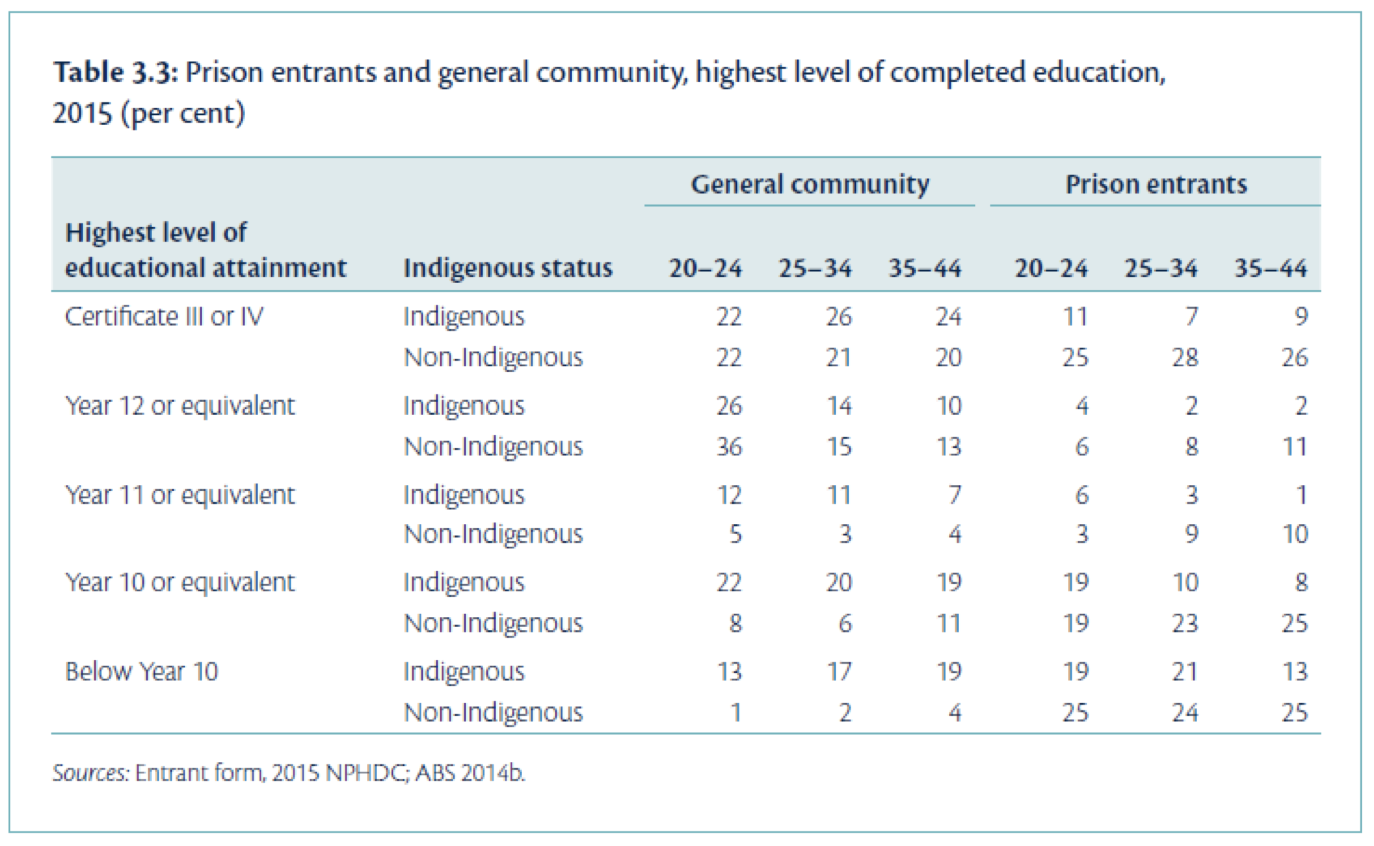
\includegraphics[width=0.66\linewidth]{img/mod01/prisoner-education} \caption{Highest level of completed education in prison entrants and the general community}\label{fig:fig-prison-education}
\end{figure}

Source: Australian Institute of Health and Welfare 2015. The health of Australia's prisoners 2015. Cat. no. PHE 207. Canberra: AIHW.

Some issues in this table:

\begin{itemize}
\tightlist
\item
  The title of the table does not contain full information about the variables in the table;
\item
  It is unclear how the percentages were calculated (which groupings added to 100\%);
\item
  The ages are not labelled as such, thus without reading the text in report it is unclear that these are age groupings.
\end{itemize}

\hypertarget{table-presentation-guidelines-woodward-2013}{%
\subsection{Table presentation guidelines (Woodward, 2013)}\label{table-presentation-guidelines-woodward-2013}}

\begin{enumerate}
\def\labelenumi{\arabic{enumi}.}
\tightlist
\item
  Each table (and figure) should be self-explanatory, i.e.~the reader should be able to understand it without reference to the text in the body of the report.

  \begin{itemize}
  \tightlist
  \item
    This can be achieved by using complete, meaningful labels for the rows and columns and giving a complete, meaningful title.
  \item
    Footnotes can be used to enhance the explanation.
  \end{itemize}
\item
  Units of the variables (and if needed, method of calculation or derivation) should be given and missing records should be noted (e.g.~in a footnote).
\item
  A table should be visually uncluttered.

  \begin{itemize}
  \tightlist
  \item
    Avoid use of vertical lines.
  \item
    Horizontal lines should not be used in every single row, but they can be used to group parts of the table.
  \item
    Sensible use of white space also helps enormously; use equal spacing except where large spaces are left to separate distinct parts of the table.
  \item
    Different typefaces (or fonts) may be used to provide discrimination, e.g.~use of bold type and/or italics.
  \end{itemize}
\item
  The rows and columns of each table should be arranged in a natural order to help interpretation. For instance, when rows are ordered by the size of the numbers they contain for a nominal variable, it is immediately obvious where relatively big and small contributions come from.
\item
  Tables should have a consistent appearance throughout the report so that the paper is easy to follow (and also for an aesthetic appearance). Conventions for labelling and ordering should be the same (for both tables as well as figures) for ease of comparison of different tables (and figures).
\item
  Consider if there is a particular table orientation that makes a table easier to read.
\end{enumerate}

Given the different possible formats of tables and their complexity, some further guidelines are given in the following excellent references:

\begin{itemize}
\tightlist
\item
  Graphics and statistics for cardiology: designing effective tables for presentation and publication, \citet{boers18}
\item
  Guidelines for Reporting of Figures and Tables for Clinical Research in Urology, \citet{vickers_etal20}
\end{itemize}

\hypertarget{graphical-presentation}{%
\section{Graphical presentation}\label{graphical-presentation}}

\hypertarget{bar-graphs}{%
\subsection{Bar graphs}\label{bar-graphs}}

Using the PBC data from the Introduction to Stata exercise, we can present the distribution of Stage of Disease graphically using a bar graph. Bar graphs, which are suitable for plotting discrete or categorical variables, are defined by the fact that the bars do not touch.

\begin{figure}[H]
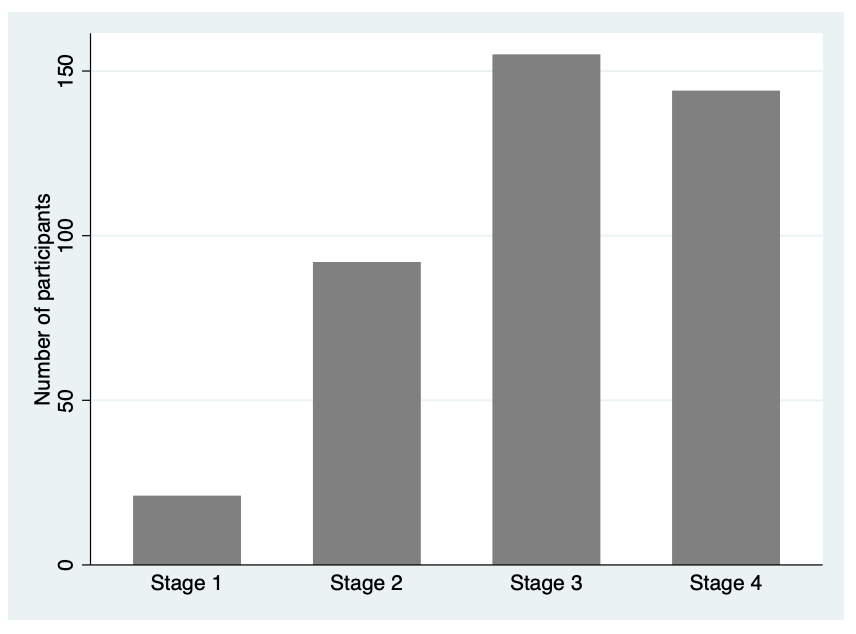
\includegraphics[width=0.75\linewidth]{img/mod01/pbc-bar} \caption{Bar graph of stage of disease from PBC study}\label{fig:fig-1-1}
\end{figure}

Information from more than one variable can be presented as clustered or multiple bar chart (bars side-by-side) (Figure \ref{fig:fig-1-2}). This type of graph is useful when examining changes in the categories separately, but also comparing the grouping variable between the main bar variable. Here we can see that Stage 3 and Stage 4 disease is the most common for both males and females, but there are many more females within each stage of disease.

\begin{figure}[H]
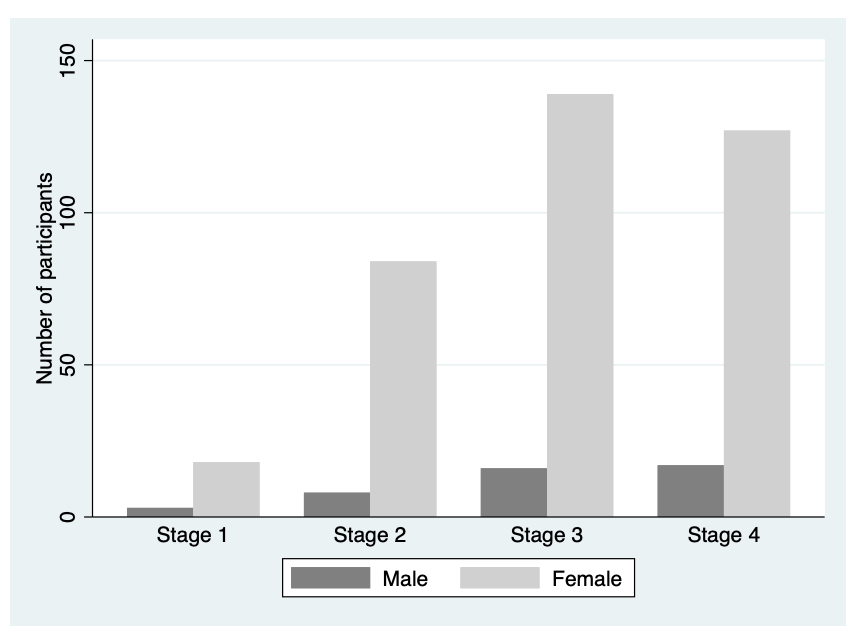
\includegraphics[width=0.75\linewidth]{img/mod01/pbc-bar-stage-sex} \caption{Bar graph of stage of disease by sex from PBC study}\label{fig:fig-1-2}
\end{figure}

An alternative bar graph is a stacked or composite bar graph, which retains the overall height for each category, but differentiates the bars by another variable (Figure \ref{fig:fig-1-3}).

\begin{figure}[H]
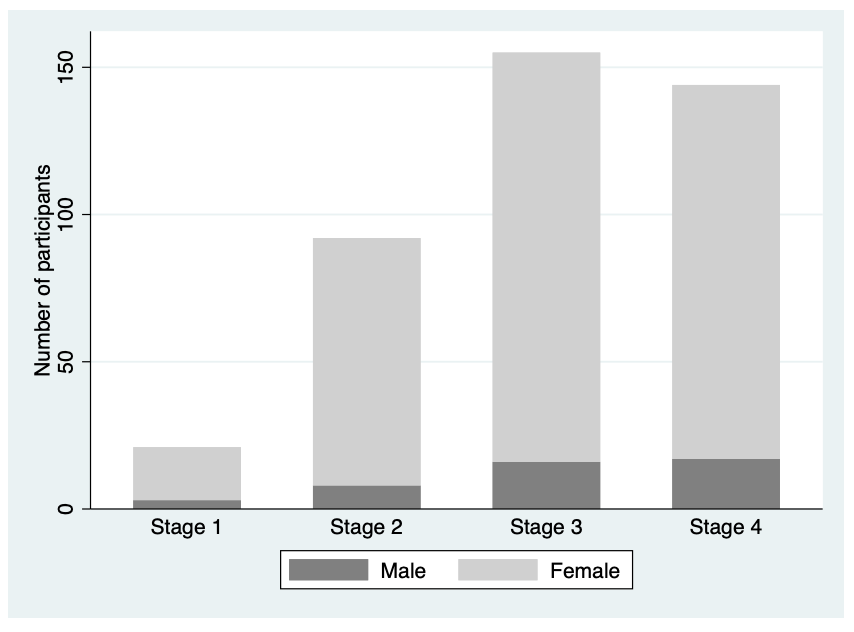
\includegraphics[width=0.75\linewidth]{img/mod01/pbc-bar-stage-sex-stacked} \caption{Stacked bar graph of stage of disease by sex from PBC study}\label{fig:fig-1-3}
\end{figure}

Finally, a stacked relative bar chart (Figure \ref{fig:fig-1-4}) displays the proportion of grouping variable for each bar, where each overall bar represents 100\%. These graphs allow the reader to compare the proportions between categories. We can easily see from Figure \ref{fig:fig-1-4} that the distribution of sex is similar across each stage of disease.

\begin{figure}[H]
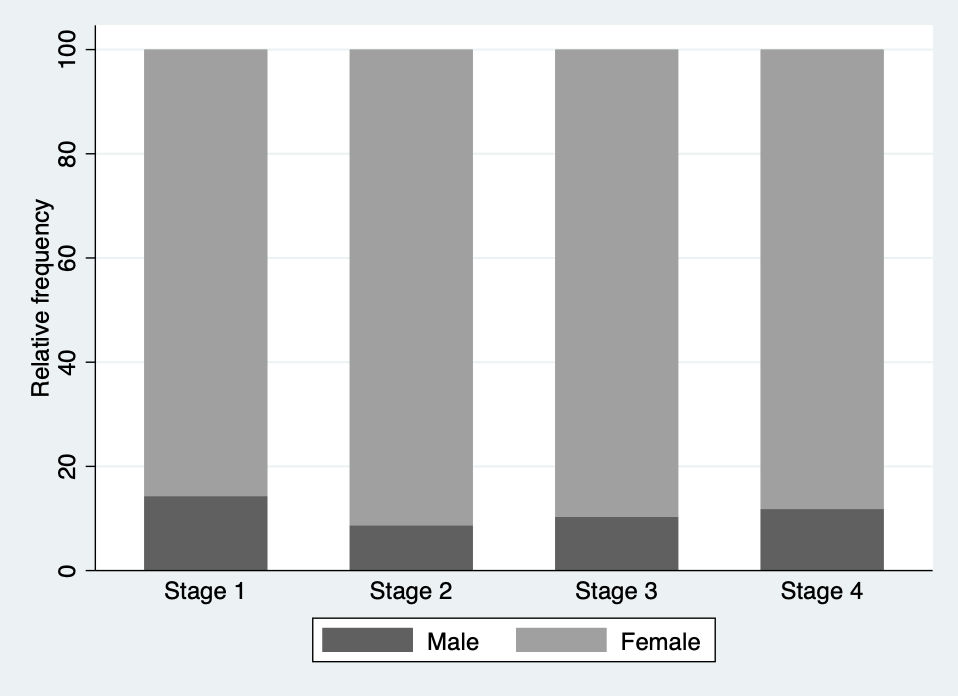
\includegraphics[width=0.75\linewidth]{img/mod01/pbc-bar-stage-sex-stacked-relative} \caption{Relative frequency of sex within stage of disease from PBC study}\label{fig:fig-1-4}
\end{figure}

\hypertarget{line-graphs}{%
\subsection{Line graphs}\label{line-graphs}}

A line graph is effective to illustrate trends over time (e.g.~change over several years). Let's look at an example from cancer epidemiology.

Cancer incidence is the number of new cases of cancer diagnosed in a population in a given time period. A useful comparison with the incidence rate is the mortality rate, revealing information about the deaths from cancer in the same period. Figure \ref{fig:fig-1-5} shows the prostate cancer trend in the NSW male population in the period 1972-2014, specifically the age-standardised incidence and mortality rate per 100,000.

\begin{figure}[H]
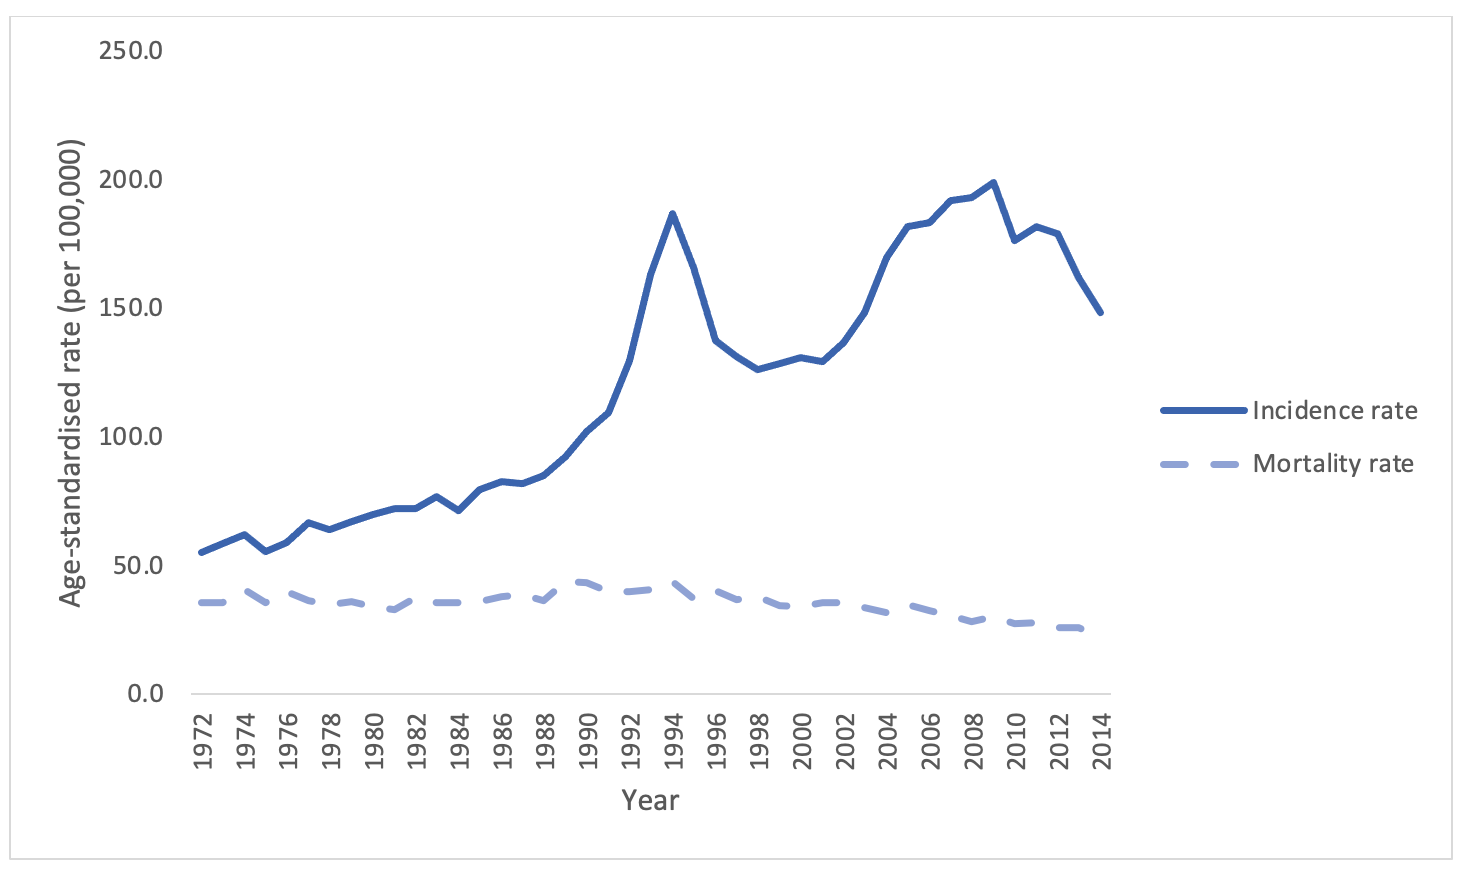
\includegraphics[width=0.66\linewidth]{img/mod01/line-graph-prostate-cancer} \caption{Prostate cancer age-standardised incidence and mortality rates (per 100,000), NSW, 1972-2014}\label{fig:fig-1-5}
\end{figure}

Source: The Cancer Institute NSW (2018) Cancer statistics NSW. \url{https://www.cancer.nsw.gov.au/cancer-statistics-nsw} (Accessed: 24 Jan 2019).

The age standardised incidence rate for prostate cancer increased steadily in the period 1972 -- 1991, from 55.2 cases per 100,00 to 109.3 cases per 100,000. There were two notable peaks in incidence in the period 1972-2014. In particular, there was an increase between 1992-1994, and also between 2002-2009. Since 2009 (to 2014) the rates decreased from 198.9 per 100,000 to 148.2 per 100,000. Whilst the incidence rate for prostate cancer has fluctuated over the period, the age standardised mortality rate remained relatively stable (around 35 deaths per 100,000). Since 2009 the mortality rate appears to be decreasing and was at its lowest in 2014 at 22.1 per 100,000.

{[}The increase in prostate cancer incidence in the early 1990's occurred at a time when blood testing of men for Prostate Specific Antigen (PSA) became more widespread. The more recent peak in incidence in the early 2000's maybe explained by PSA being increasingly used as a screening test for men who did not have symptoms of prostate cancer.{]}

\hypertarget{pie-charts}{%
\subsection{Pie charts}\label{pie-charts}}

An example of graphical presentation that we would recommend avoiding, is a pie chart. These are often used to present the proportion of each category that contributed to the total. However, their use is limited and sometimes misleading, and the same information can be presented as a stacked bar chart of proportions. Here are some reasons why not to use pie charts:

\begin{itemize}
\tightlist
\item
  Not ideal when there are many categories to compare
\item
  The use of percentages is not appropriate when the sample size is small
\item
  Can be misleading by using different size pies, different rotations and different colours to draw attention to specific groups
\item
  3D and exploding bar charts further distort the effect of perspective and may confuse the reader
\end{itemize}

\hypertarget{graphical-presentation-guidelines}{%
\subsection{Graphical presentation guidelines}\label{graphical-presentation-guidelines}}

Consider the following guidelines for the appropriate presentation of graphs in scientific journals and reports (Woodward, 2013).

\begin{itemize}
\tightlist
\item
  Figures should be self-explanatory and have consistent appearance through the report.
\item
  A title should give complete information. Note that figure titles are usually placed below the figure, whereas for tables titles are given above the table.
\item
  Axes should be labelled appropriately
\item
  Units of the variables should be given in the labelling of the axes. Use footnotes to indicate any calculation or derivation of variables and to indicate missing values
\item
  If the Y-axis has a natural origin, it should be included, or emphasised if it is not included.
\item
  If graphs are being compared, the Y-axis should be the same across the graphs to enable fair comparison
\item
  Columns of bar charts should be separated by a space
\item
  Three dimensional graphs should be avoided unless the third dimension adds additional information
\end{itemize}

\hypertarget{summary-statistics-and-variation-in-data}{%
\section{Summary statistics and variation in data}\label{summary-statistics-and-variation-in-data}}

We often collect measurements that are continuous in nature, that is measurements such as height, weight, time, blood pressure etc which can be measured accurately to one or more decimal places. A useful way of describing the continuous data is via summary statistics. These include measures to describe the distribution of data points via the central tendency (e.g.~mean, median) and spread (e.g.~standard deviation and inter quartile range). We also examine the data visually by graphing it using histograms and box plots.

\hypertarget{mathematical-and-statistical-notation}{%
\subsection{Mathematical and statistical notation}\label{mathematical-and-statistical-notation}}

When computing summary statistics or using more formal statistical methods, mathematical and statistical notation is often used. Below are some of the common statistical terms and interpretation that will be used in the course and which are seen in many text books.

\begin{longtable}[]{@{}ll@{}}
\toprule()
Notation & Interpretation \\
\midrule()
\endhead
\(x\) & An observation in your sample \\
\(\sum x\) & Sum of all the observations \\
\(N\) & Total population size \\
\(n\) & Sample size \\
\(\mu\) (mu) & Population mean \\
\(\sigma^2\) & Population variance \\
\(\sigma\) & Population standard deviation \\
\(\bar{x}\) & Sample mean \\
\(s^2\) & Sample variance \\
\(s\) & Sample standard deviation \\
\bottomrule()
\end{longtable}

\hypertarget{measures-of-central-tendency}{%
\subsection{Measures of central tendency}\label{measures-of-central-tendency}}

\hypertarget{worked-example-1}{%
\subsubsection{Worked example}\label{worked-example-1}}

In our random sample of 30 students attending a university gym on a given day, their weight in kilograms was measured (see below). Weight is a continuous measurement (similar to height, blood pressure etc) that in theory can be measured to infinitely small units, though in practice they can be measured accurately to one or two decimal places.

We will use these data to look at measures of central tendency and spread of the data and other summary statistics.

60.0\\
62.5 62.5 62.5\\
65.0 65.0 65.0\\
67.5 67.5 67.5 67.5 67.5\\
70.0 70.0 70.0 70.0 70.0 70.0
72.5 72.5 72.5 72.5\\
75.0 75.0 75.0 75.0 75.0\\
77.5 77.5\\
80.0

\hypertarget{mean}{%
\subsubsection{Mean}\label{mean}}

The most commonly used measure of the central tendency of the data is the mean value. The mean of a set of values is often referred to as the average of all the values. The mean (\(\bar{x}\)) of a sample dataset is calculated using the following formula:

\[\bar{x} = \frac{\sum x}{n}\]

From the weights example: \(\bar{x}\) = 2100/30 = 70.0. Thus, the mean weight of this sample is 70.0 kg

\hypertarget{median-and-mode}{%
\subsubsection{Median and mode}\label{median-and-mode}}

Other measures of central tendency include the median and mode. The median is the true centre of the data, the value at which half of the measurements lie above it and half of the measurements lie below it.

To estimate the median, the data are ordered from the lowest to highest values, and the middle value is used. If the middle value is between two data points (if there are an even number of observations), the median is an average of the two values.
Using the weight example, the median would be 70.0 kg.

For a set of eight exam results ranked in order:

48 51 55 59 63 64 69 75

The median is the average of the two middle observations: 59 and 63. So the median is (59+63)/2 = 61

The mode is the most frequent value in the distribution, in the weight example this would be 70.0 kg as this value features most frequently. The mode is not used frequently.

\hypertarget{describing-the-spread-of-the-data}{%
\subsection{Describing the spread of the data}\label{describing-the-spread-of-the-data}}

In addition to measuring the centre of the data, we also need a robust estimate of the spread of the data points.

\hypertarget{range}{%
\subsubsection{Range}\label{range}}

The absolute measure of the spread of the data is the range, that is the difference between the highest and lowest values in the dataset.

Range = highest data value -- lowest data value

Using the weights example, Range = 80.0 - 60.0 = 20.0 kg

Note that while the range is 20.0 kg, the range is often reported as the actual lowest and highest values e.g.~Range 60 to 80 kg.

The range is not always ideal as it only describes the extreme values, without considering how the bulk of the data is distributed between them.

\hypertarget{variance-and-standard-deviation}{%
\subsubsection{Variance and standard deviation}\label{variance-and-standard-deviation}}

More useful statistics to describe the spread of the data around a mean value are the variance and standard deviation. These measures of variability depend on the difference between individual observations and the mean value (deviations). If all values are equal to the mean there would be no variability at all, all deviations would be zero; conversely large deviations indicate greater variability.

One way of combining deviations in a single measure is to first square the deviations and then average the squares. Squaring is done because we are equally interested in negative deviations and positive deviations; if we averaged without squaring, negative and positive deviations would `cancel out'. This measure is called the variance of the set of observations. It is `the average squared deviation from the mean'. Because the variance is in `square' units and not in the units of the measurement, a second measure is derived by taking the square root of the variance. This is the standard deviation (SD), and is the most commonly used measure of variability in practice, as it is a more intuitive interpretation since it is in the same units as the units of measurement (adapted from: Williams, 2015).

The formula for the variance of a sample (\(s^2\)) is:

\[ s^2 = \frac{\sum(x - \bar{x})^2}{n-1} \]

Note that the deviations are first squared before they are summed to remove the negative values; once summed they are divided by the sample size minus 1.

The sample standard deviation is the square root of the of the sample variance:

\[s = \sqrt{s^2}\]
For the worked weights example, we would calculate the sample variance:

\[\begin{aligned}
  s^2 &= \frac{(60.0 - 70.0)^2 + (62.5 - 70.0)^2 + \dots + (80.0 - 70.0)^2}{30-1} \\
      &= \frac{737.5}{29} \\
      &= 25.43 \text{ kg}^2
  \end{aligned}\]

with a sample standard deviation: \(s = \sqrt{25.43} = 5.04 \text{ kg}\).

Thus, in our sample of 30 students, we have an estimated mean weight of 70.0 kg, with a variance of 25.43 kg\textsuperscript{2} and a standard deviation of 5.04 kg.

Characteristics of the standard deviation
- It is affected by every measurement
- It is in the same units as the measurements
- It can be converted to measures of precision (standard error and 95\% confidence intervals) (Module 3)

Interquartile range
The inter-quartile range (IQR) describes the range of measurements in the central 50\% of values around the median i.e.~the bottom 25\% and top 25\% of values are discarded and only the values in the 25\%-75\% range are quoted. The IQR is the preferred measure of spread when the median has been used to describe central tendency.

In the weights example the IQR would be 67.5 -- 75.0 (i.e.~the middle 50\% of values).

\hypertarget{population-values-mean-variance-and-standard-deviation}{%
\section{Population values: mean, variance and standard deviation}\label{population-values-mean-variance-and-standard-deviation}}

The examples above show how the sample mean, range, variance and standard deviation are calculated from the sample of weight measures from 30 people. If we had information on the weight of the total population that the sample was drawn from, we could calculate all the summary statistics described above (for the sample) for the population.

The equation for calculating the population mean is the same as that of sample mean, though now we denote the population mean as μ:

\[ \mu = \frac{\sum{x}}{N} \]

Where \(\sum{x}\) represents the sum of the values in the population, and \(N\) represents the total number of measurements in the population.

To calculate the population variance (\(\sigma^2\)) and standard deviation(\(\sigma\)), we use a slightly modified version of the equation for \(s^2\):

\[ \sigma^2 = \frac{\sum(x - \mu)^2}{N} \]

with a population standard deviation of: \(\sigma = \sqrt{\sigma^2}\).

In practice, we rarely have the information for the entire population to be able to calculate the population mean and standard deviation. Theoretically, however, these statistics are important for two main purposes:

\begin{enumerate}
\def\labelenumi{\arabic{enumi}.}
\tightlist
\item
  the characteristics of the normal distribution (the most important probability distribution discussed in later modules) are defined by the population mean and standard deviation;
\item
  while calculating sample sizes (discussed in later modules) we need information about the population standard deviation, which is usually obtained from the existing literature.
\end{enumerate}

\hypertarget{using-graphs-to-display-the-centre-and-spread-of-the-data}{%
\section{Using graphs to display the centre and spread of the data}\label{using-graphs-to-display-the-centre-and-spread-of-the-data}}

As well as calculating measures of central tendency and spread to describe the characteristics of the data, a graphical plot is very helpful to better understand the characteristics and distribution of the measurements obtained. \emph{Histograms} and \emph{box plots} are excellent ways to graphically display continuous data.

\hypertarget{frequency-histograms}{%
\subsection{Frequency histograms}\label{frequency-histograms}}

A histogram that plots the frequency of the grouped observations is called a frequency histogram. Some features of a frequency histogram:

\begin{itemize}
\tightlist
\item
  The area under each rectangle is proportional to the frequency
\item
  The rectangles are drawn without gaps between them (unlike a bar graph)
\item
  The data are `binned' into discrete intervals (of (usually of equal width)
\item
  The mid-point of the histogram represents the centre (mean, median) of the data
\end{itemize}

If the rectangles are symmetrically distributed about the middle of the histogram, we say that the data are symmetric, and the mean and median will be approximately equal.

If the histogram has a longer tail to the right, then the data are said to be positively skewed (or skewed to the right), and the mean will be greater than the median.

If the histogram has an extended tail to the left, then the data are negatively skewed (or skewed to the left) and the mean will be smaller than the median.

\begin{quote}
The skewness of a distribution is defined by the location of the longer tail, not the location of the peak of the data.
\end{quote}

Figure \ref{fig:fig-1-6} presents two histograms from the PBC data from the Introduction to Stata exercise: for age and serum bilirubin. We can see that the distribution for age is roughly symmetric, while the distribution for serum bilirubin is highly positively skewed (or skewed to the right).

\begin{figure}
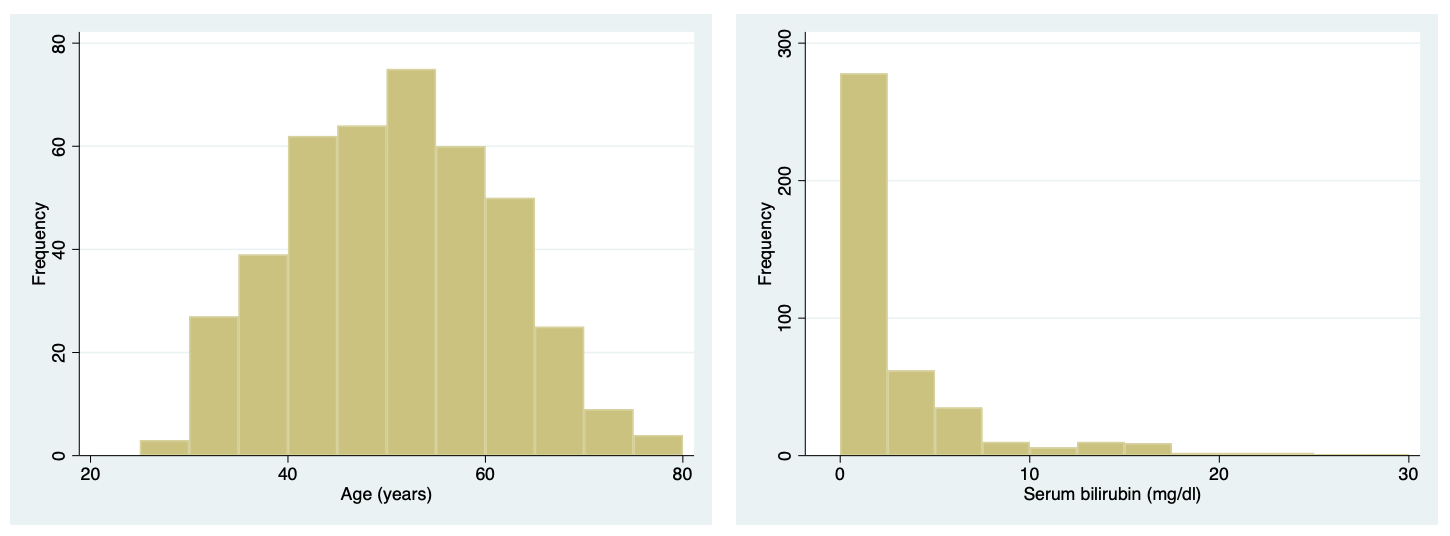
\includegraphics[width=1\linewidth]{img/mod01/hist-symmetric-skewed} \caption{Histogram of age (left) and serum bilirubin (right) from PBC study data}\label{fig:fig-1-6}
\end{figure}

\hypertarget{boxplots}{%
\subsection{Boxplots}\label{boxplots}}

Another useful way to inspect the distribution of data is by using a box plot. In a box plot:

\begin{itemize}
\tightlist
\item
  the line across the box shows the median value
\item
  the limits of the box show the 25-75\% range (i.e.~the inter-quartile range (IQR) where the middle 50\% of the data lie)
\item
  the bars (or whiskers) indicate the most extreme values (highest and lowest) that fall within 1.5 times the interquartile range from each end of the box

  \begin{itemize}
  \tightlist
  \item
    the upper whisker is the highest value falling within 75th percentile plus 1.5 × IQR
  \item
    the lower whisker is the lowest value falling within 25th percentile minus 1.5 × IQR
  \end{itemize}
\item
  any values in the dataset lying outside the whiskers are plotted individually.
\end{itemize}

If the data are symmetric, the line across the box (the median value) will be in the centre of the box, and the tails will be roughly equal.

Figure \ref{fig:fig-1-7} presents two boxplots from the PBC data: for age and serum bilirubin. We can see that the boxplot for age has roughly equal tails, and the median (the horizontal line) lies roughly in the middle of the interquartile range (the shaded box). It would be reasonable to assume that age follows a symmetric distribution from this plot. The boxplot for serum bilirubin shows a much longer upper tail, and a median much closer to the bottom of the shaded box than the middle. The boxplot also shows a number of points above the 75th percentile plus 1.5 × IQR. As the upper tail is longer than the lower tail, this distribution is positively skewed.

\begin{figure}
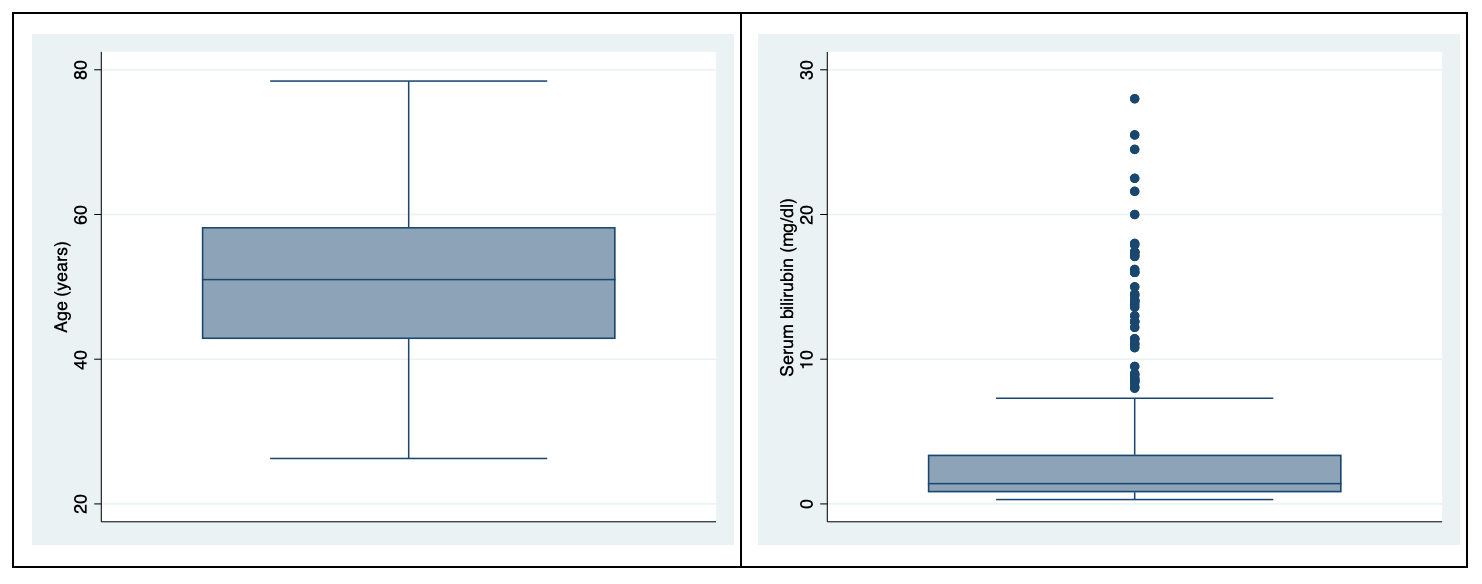
\includegraphics[width=1\linewidth]{img/mod01/boxp-symmetric-skewed} \caption{Box plot of age (left) and serum bilirubin (right) from PBC study data}\label{fig:fig-1-7}
\end{figure}

\hypertarget{how-to-report-summary-statistics}{%
\section{How to report summary statistics}\label{how-to-report-summary-statistics}}

When reporting summary statistics, it is important not to present results with too many decimal places. Doing so implies that your data have a higher level of precision than they do. For example, presenting a mean blood pressure of 100.2487 mmHg implies that blood pressure can be measured accurately to at least three decimal places.

There are a number of guidelines that have been written to help in the presentation of numerical data. Many of these guidelines are based on the number of decimal places, while others are based on the number of significant figures. Briefly, the number of significant figures are ``the number of digits from the first non-zero digit to the last meaningful digit, irrespective of the position of the decimal point. Thus, 1.002, 10.02, 100200 (if this number is expressed to the nearest 100) all have four significant digits.'' \citet{armitage_etal13}

A summary of these guidelines that will be used in this course appear below.

\begin{longtable}[]{@{}
  >{\raggedright\arraybackslash}p{(\columnwidth - 2\tabcolsep) * \real{0.2908}}
  >{\raggedright\arraybackslash}p{(\columnwidth - 2\tabcolsep) * \real{0.7092}}@{}}
\toprule()
\begin{minipage}[b]{\linewidth}\raggedright
Summary statistic
\end{minipage} & \begin{minipage}[b]{\linewidth}\raggedright
Guideline (reference)
\end{minipage} \\
\midrule()
\endhead
Mean & It is usually appropriate to quote the mean to one extra decimal place compared with the raw data. (Altman) \\
Median, Interquartile range, Range & As medians, interquartile ranges and ranges are based on individual data points, these values should be presented with the same precision as the original data. \\
Percentage & Percentages do not need to be given with more than one decimal place at most. When the sample size is less than 100, no decimal places should be given. (Altman) \\
Standard deviation & ``The standard deviation should usually be given to the same accuracy as the mean, or with one extra decimal place.'' Altman \\
Standard error & As per Standard Deviation \\
Confidence interval & Use the same rule as for the corresponding effect size (be it mean, percentage, mean difference, regression coefficient, correlation coefficient or risk ratio) (Cole) \\
Test statistic & Test statistics should not be presented with more than two decimal places. \\
P-value & Report p values to a single significant figure unless the p value is close to 0.05 (say, 0.01 -- 0.2), in which case, report two significant figures. Do not report ``not significant'' for p values of 0.05 or higher. Very low p values can be reported as p \textless{} 0.001 or similar. A p value can indeed be 1, although some investigators prefer to report this as \textgreater0.9. (Assel) \\
Difference in means & As for the estimated means \\
Difference in proportions & As for the estimated proportions \\
Odds ratio / Relative risk & Hazard and odds ratios are normally reported to two decimal places, although this can be avoided for high odds ratios (Assel) \\
Correlation coefficient & One or two decimal places, or more when very close to ±1 (Cole) \\
Regression coefficient & Use one more significant figure than the underlying data (adapted from Cole) \\
\bottomrule()
\end{longtable}

Sources:

\citet{altman90}

\citet{cole15}

\citet{assel_etal19}

\hypertarget{an-introduction-to-stata}{%
\chapter*{\texorpdfstring{\textbf{1} An introduction to Stata}{1 An introduction to Stata}}\label{an-introduction-to-stata}}
\addcontentsline{toc}{chapter}{\textbf{1} An introduction to Stata}

\hypertarget{learning-outcomes-1}{%
\section*{Learning outcomes}\label{learning-outcomes-1}}
\addcontentsline{toc}{section}{Learning outcomes}

By the end of these notes, you will be able to:

\begin{itemize}
\tightlist
\item
  navigate the Stata interface
\item
  input and import data into Stata
\item
  use Stata menus to summarise data
\item
  perform basic data transformations
\item
  assign variable and value labels
\item
  understand the difference between saving data and saving Stata output
\item
  copy Stata output to a standard word processing package
\end{itemize}

\hypertarget{introduction}{%
\section*{Introduction}\label{introduction}}
\addcontentsline{toc}{section}{Introduction}

Stata is a powerful statistical package that is relatively easy to use. It is commonly used in health research, as well as in other fields such as econometrics and social science. The aim of these notes is to introduce the Stata environment, and to introduce the commands and procedures that are directly relevant to this course. There is much more to Stata that we will cover in these notes, and more information will be provided throughout the course.

\hypertarget{part-1-a-simple-stata-analysis}{%
\section*{Part 1: A simple Stata analysis}\label{part-1-a-simple-stata-analysis}}
\addcontentsline{toc}{section}{Part 1: A simple Stata analysis}

In this very brief section, we will introduce Stata by calculating the average of six ages. If you are using Windows, open Stata by clicking: \textbf{Start \textgreater{} Stata 16 \textgreater{} Stata SE}

If you are using MacOS, open Stata from the Applications folder. Note that while Stata is available for Windows and MacOS, most of the screenshots in these notes will be based on the Windows version.

When you first open Stata, it will look something like the following.

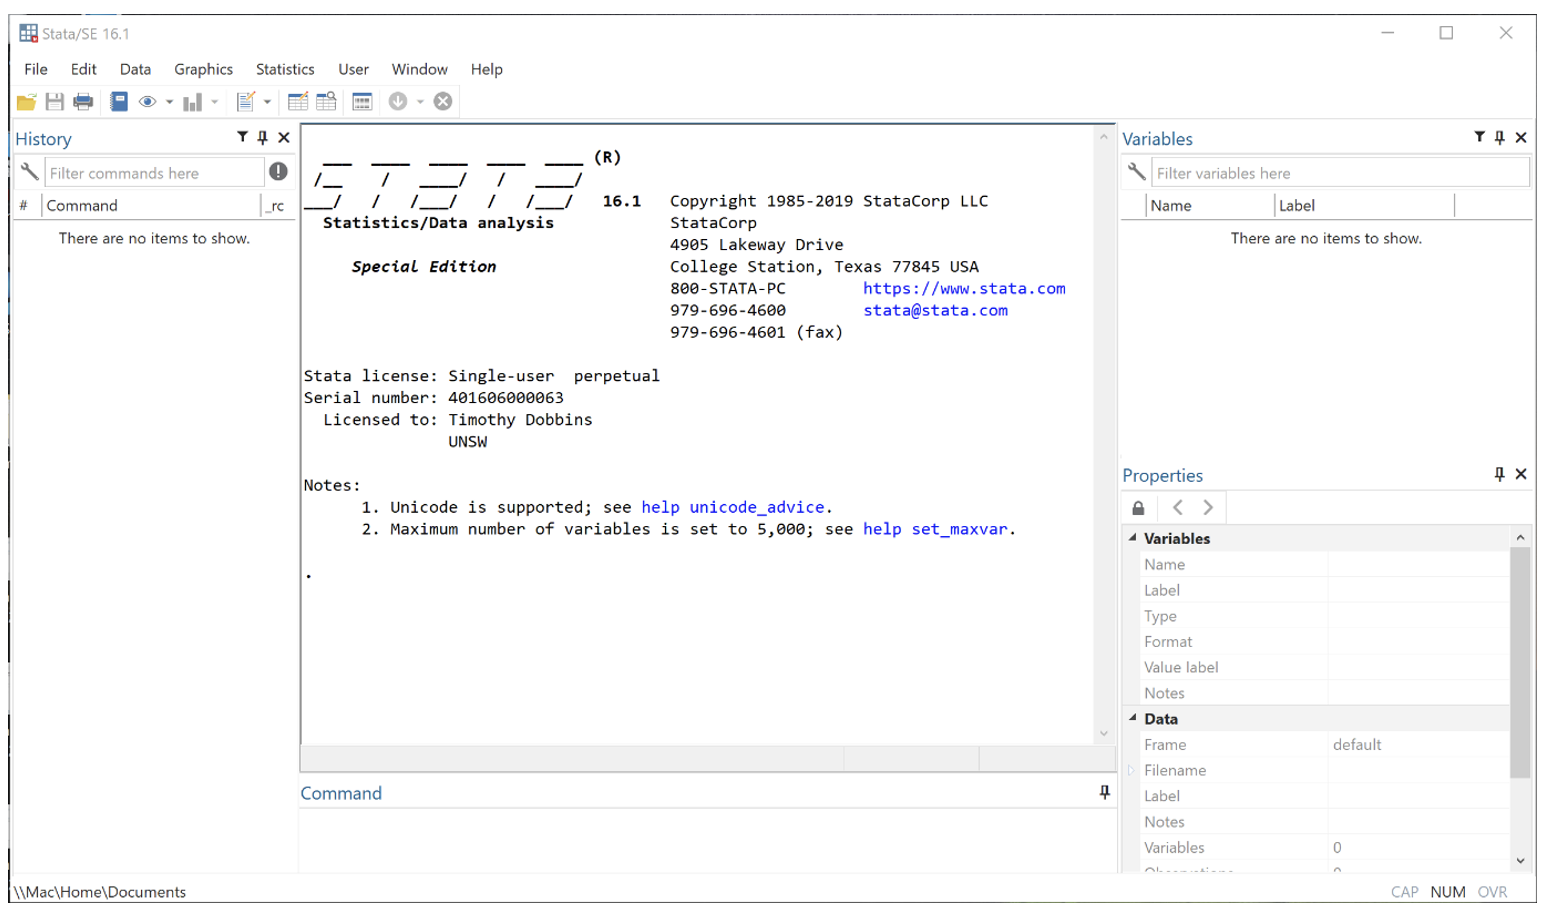
\includegraphics[width=0.75\linewidth]{img/mod01/stata/simple-01}

Each Stata session has a number of windows, which we will discuss later. For now, look in the top row of icons and find the icons that look like two grids: one with a pencil, and one with a magnifying glass: 
\includegraphics{img/mod01/stata/data-browser-icons.png}. Click the left icon, the one with the pencil. The following window will appear.

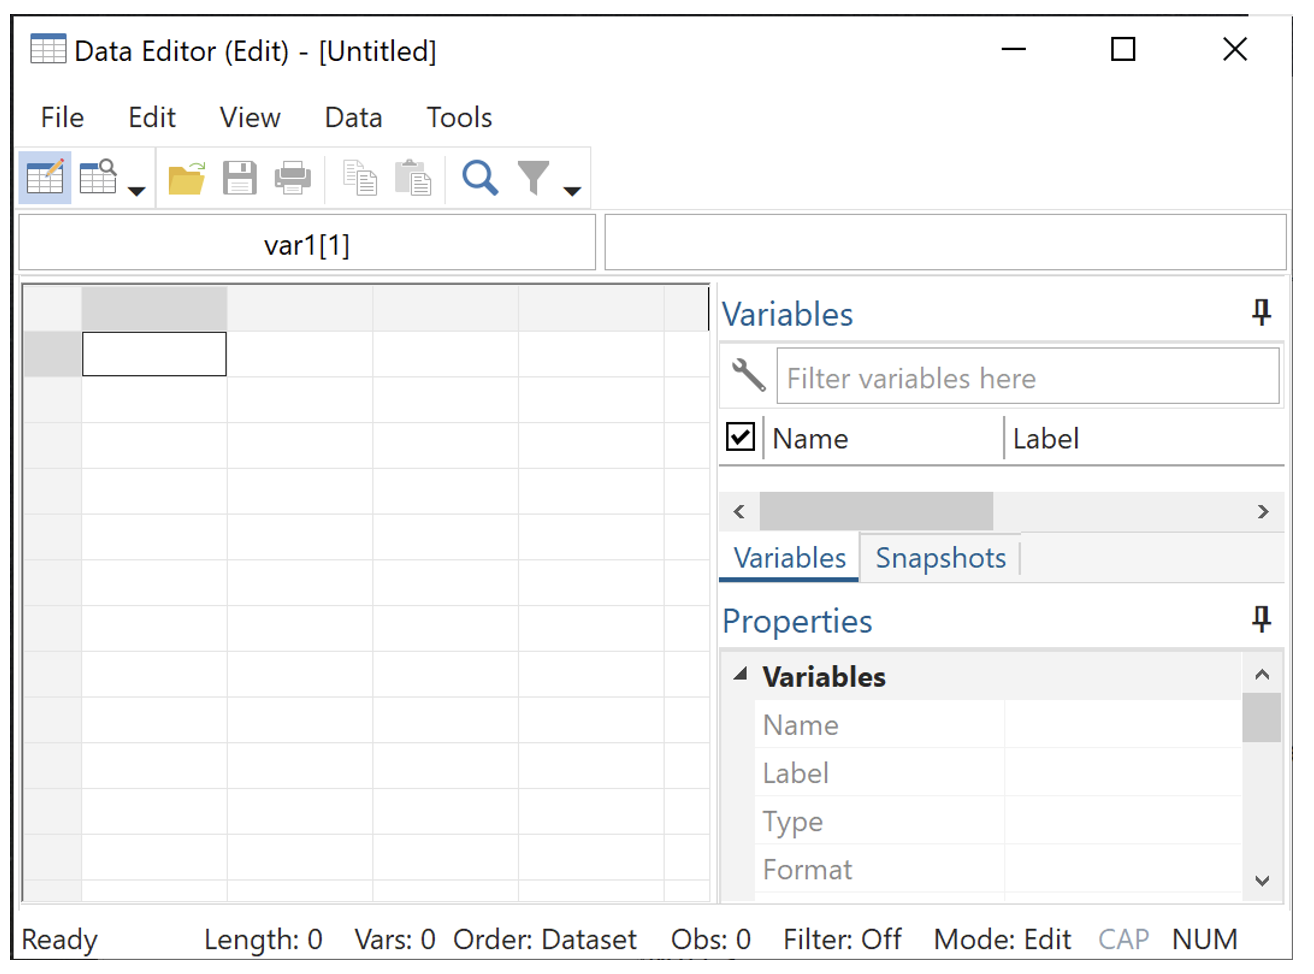
\includegraphics[width=0.75\linewidth]{img/mod01/stata/simple-02}

This window is known as the \textbf{Data Editor}, and is where data can be entered or changed. Enter the following six ages into Stata, starting at the top-left cell, by typing each number and then hitting Enter.

\begin{verbatim}
20  25  23  29  21  27
\end{verbatim}

If you make a mistake, simply click the incorrect cell, and enter the correct value. Your screen should look like this:

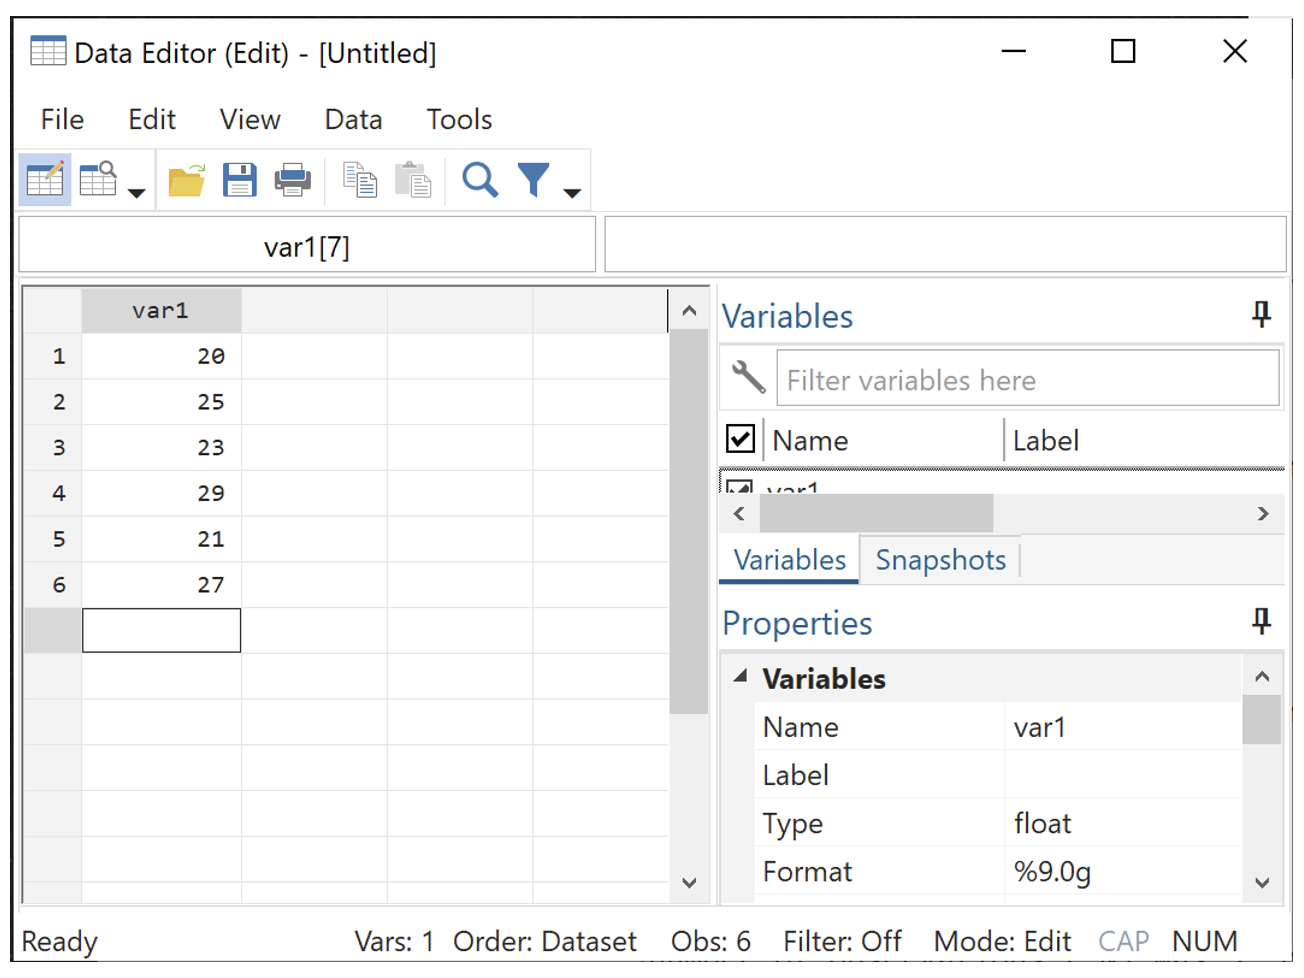
\includegraphics[width=0.75\linewidth]{img/mod01/stata/simple-03}

There are two things to note here:

\begin{enumerate}
\def\labelenumi{\arabic{enumi}.}
\tightlist
\item
  Data in Stata are entered down a column. In Stata, columns represent variables, and rows represent observations. So our six observations of age are entered in one column.
\item
  Stata has given the name of \texttt{var1} to our column of ages. We will fix this in a moment.
\end{enumerate}

Close the \textbf{Data Editor} window to return to the main Stata window. You will notice that the main Stata window now has some text that you might not understand. We will explain why shortly.

Let's rename our variable from \texttt{var1} to \texttt{age}. There are a few ways you can do this in Stata, but one of the most convenient is to use the \textbf{Variables Manager} which can be accessed via \textbf{Data \textgreater{} Variables Manager}:

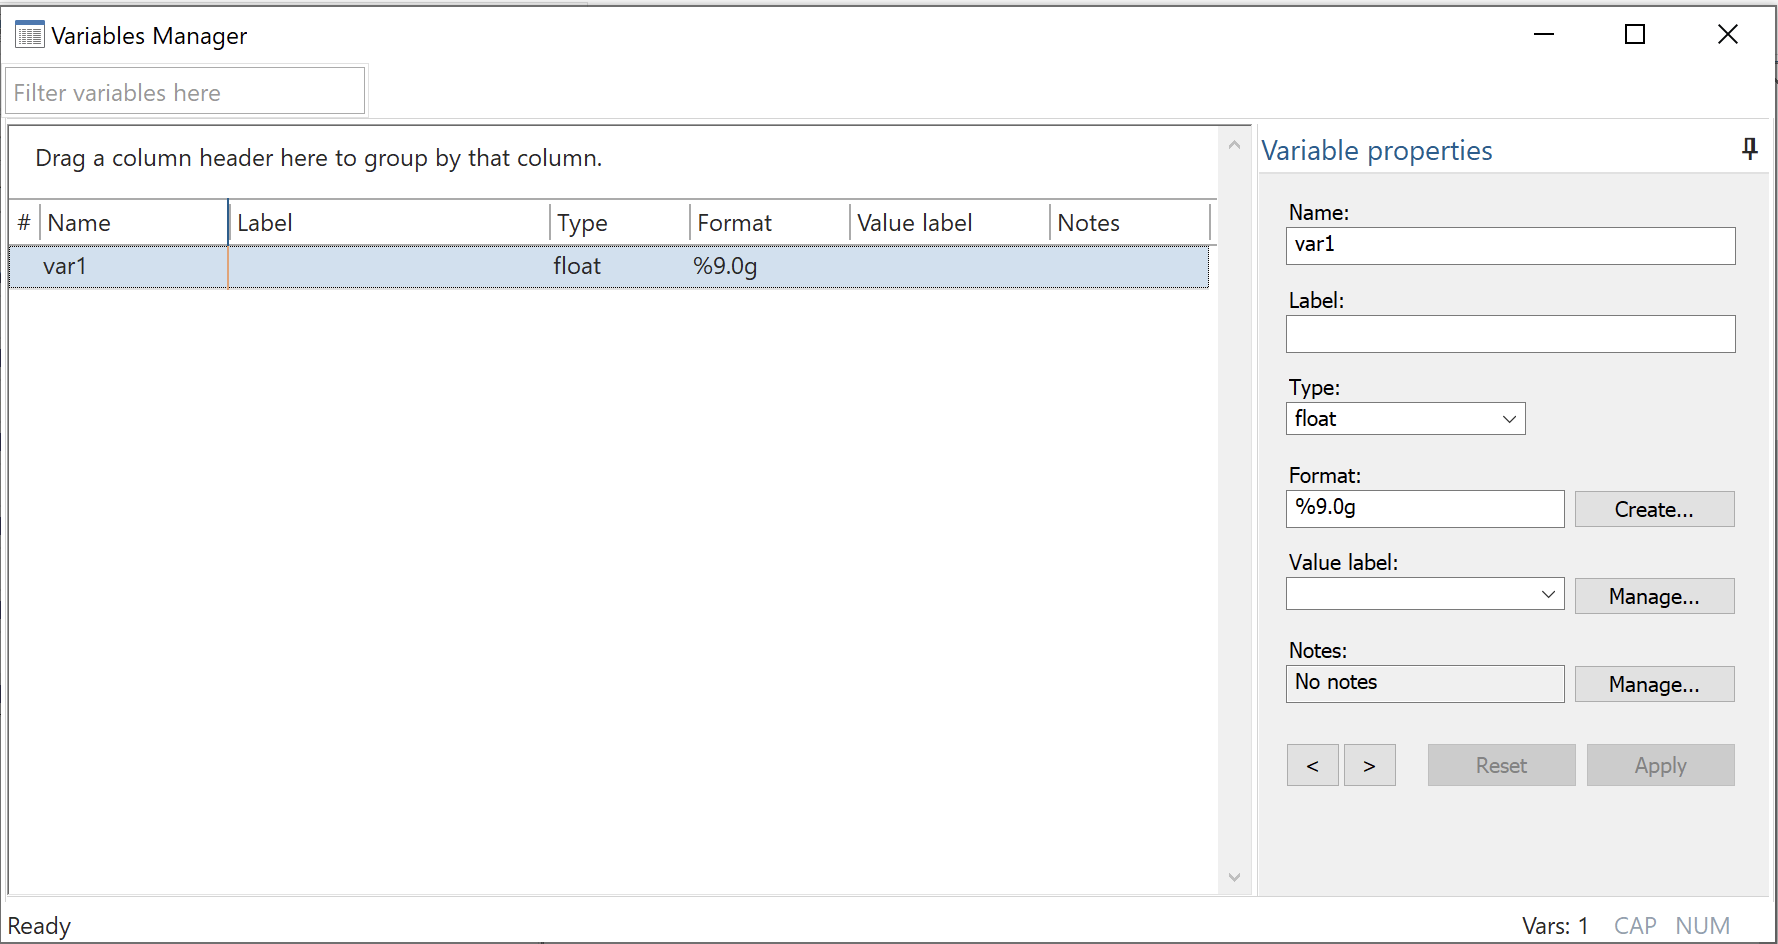
\includegraphics[width=0.75\linewidth]{img/mod01/stata/variables-manager-01}

The \textbf{Variables Manager} is where you can change many variable properties, such as variable names or apply meaningful variable labels. Each variable is listed on a separate row, with aspects about each variable listed in the columns. To change the variable name, click \texttt{var1} in the \textbf{Name} column. Notice that information about that variable appears to the right of the window, in the \textbf{Variable properties} section.

In the \textbf{Name} section within \textbf{Variable properties}, click \texttt{var1} and replace it with \texttt{age}. Click \textbf{Apply} and notice that the variable's name has been changed:

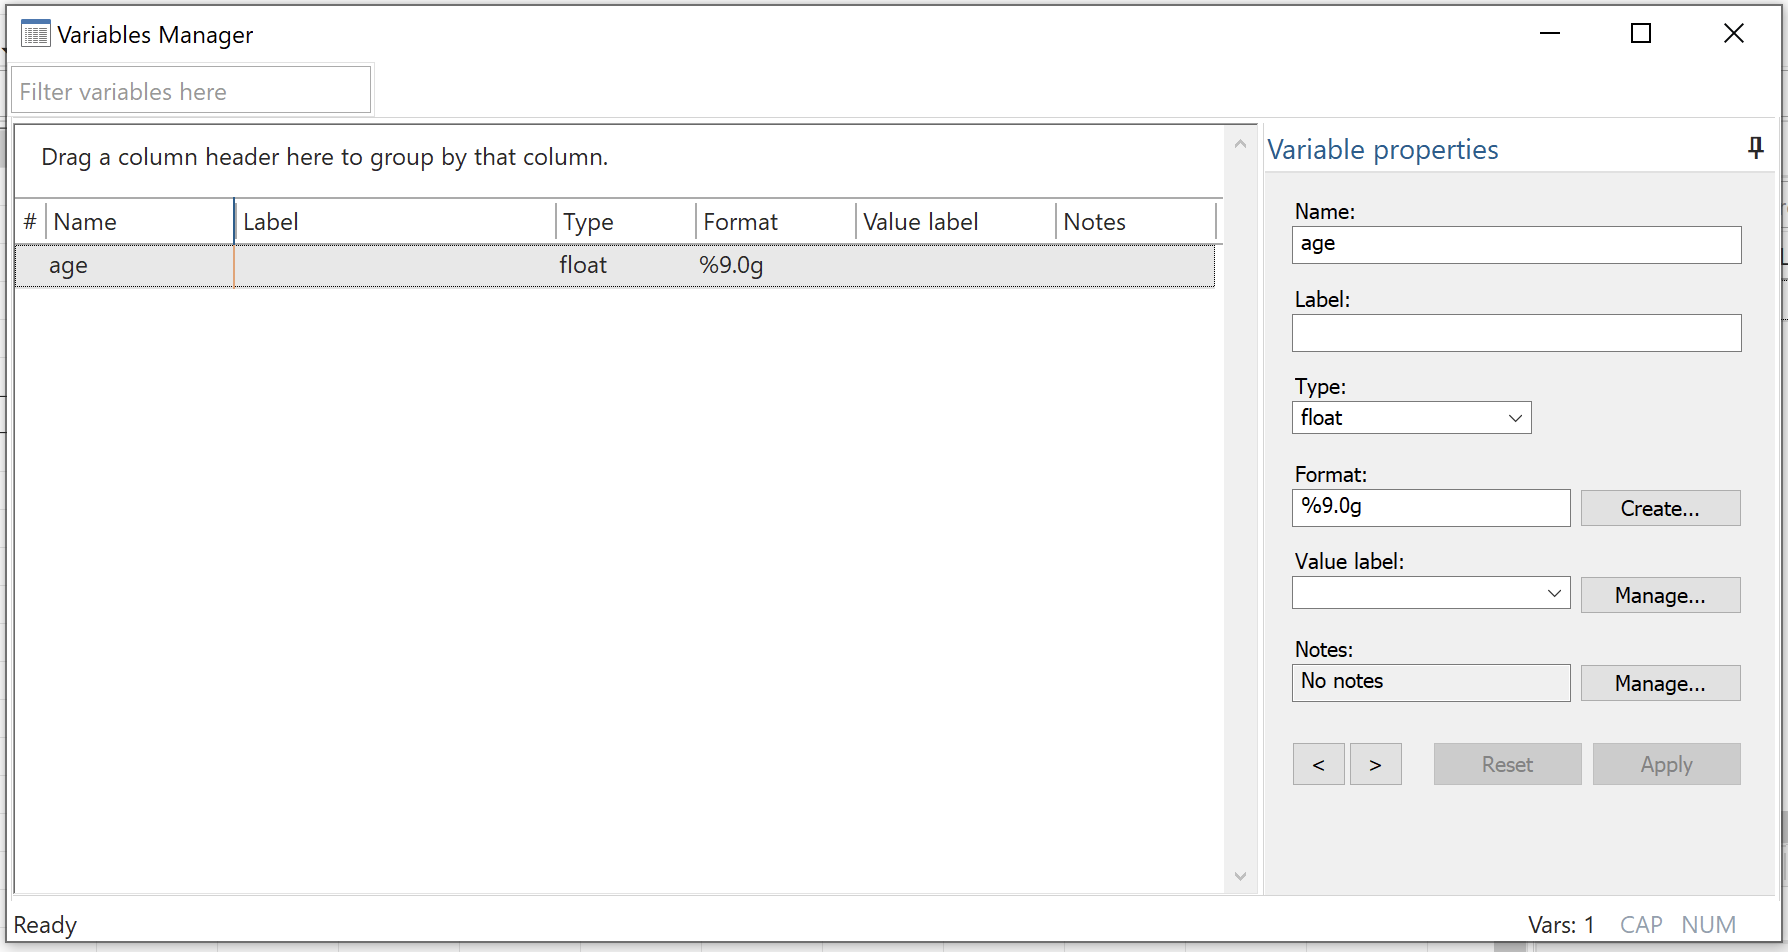
\includegraphics[width=0.75\linewidth]{img/mod01/stata/variables-manager-02}

Close the \textbf{Variables manager} window.

Some important points about variable names in Stata:
- any name you choose must be no more than 32 characters long;
- variable names must contain only letters, numbers and the underscore (\_);
- variable names should start with a letter;
- variable names are case-sensitive (so age, Age and AGE could represent three different variables)

Now that we have entered our six ages, let's calculate the mean age. Choose \textbf{Statistics \textgreater{} Summaries, tables and tests \textgreater{} Summary and descriptive statistics \textgreater{} Summary statistics}. The \textbf{summarize} dialog box will appear. From the \textbf{Variables} drop-down box, select \texttt{age} as below:

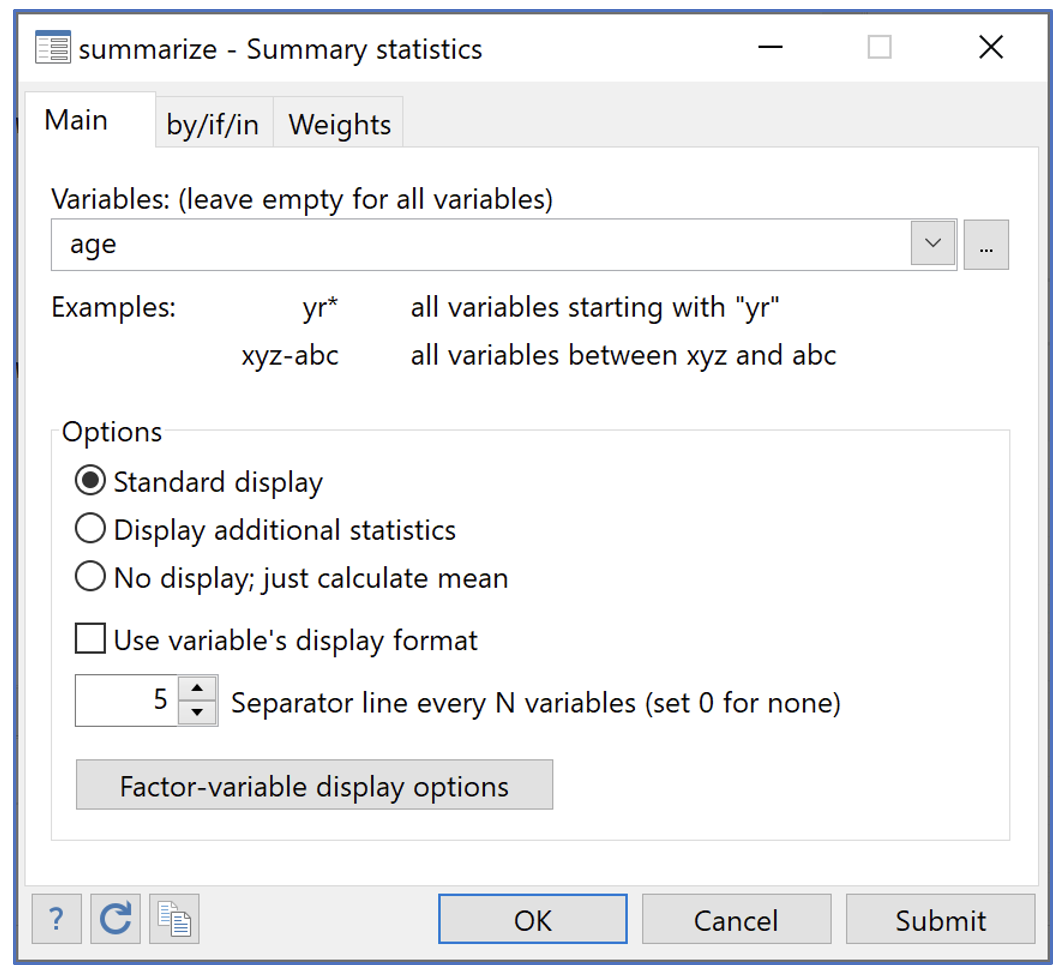
\includegraphics[width=0.75\linewidth]{img/mod01/stata/simple-05}

Click \textbf{OK}, and the main Stata screen will appear as below.

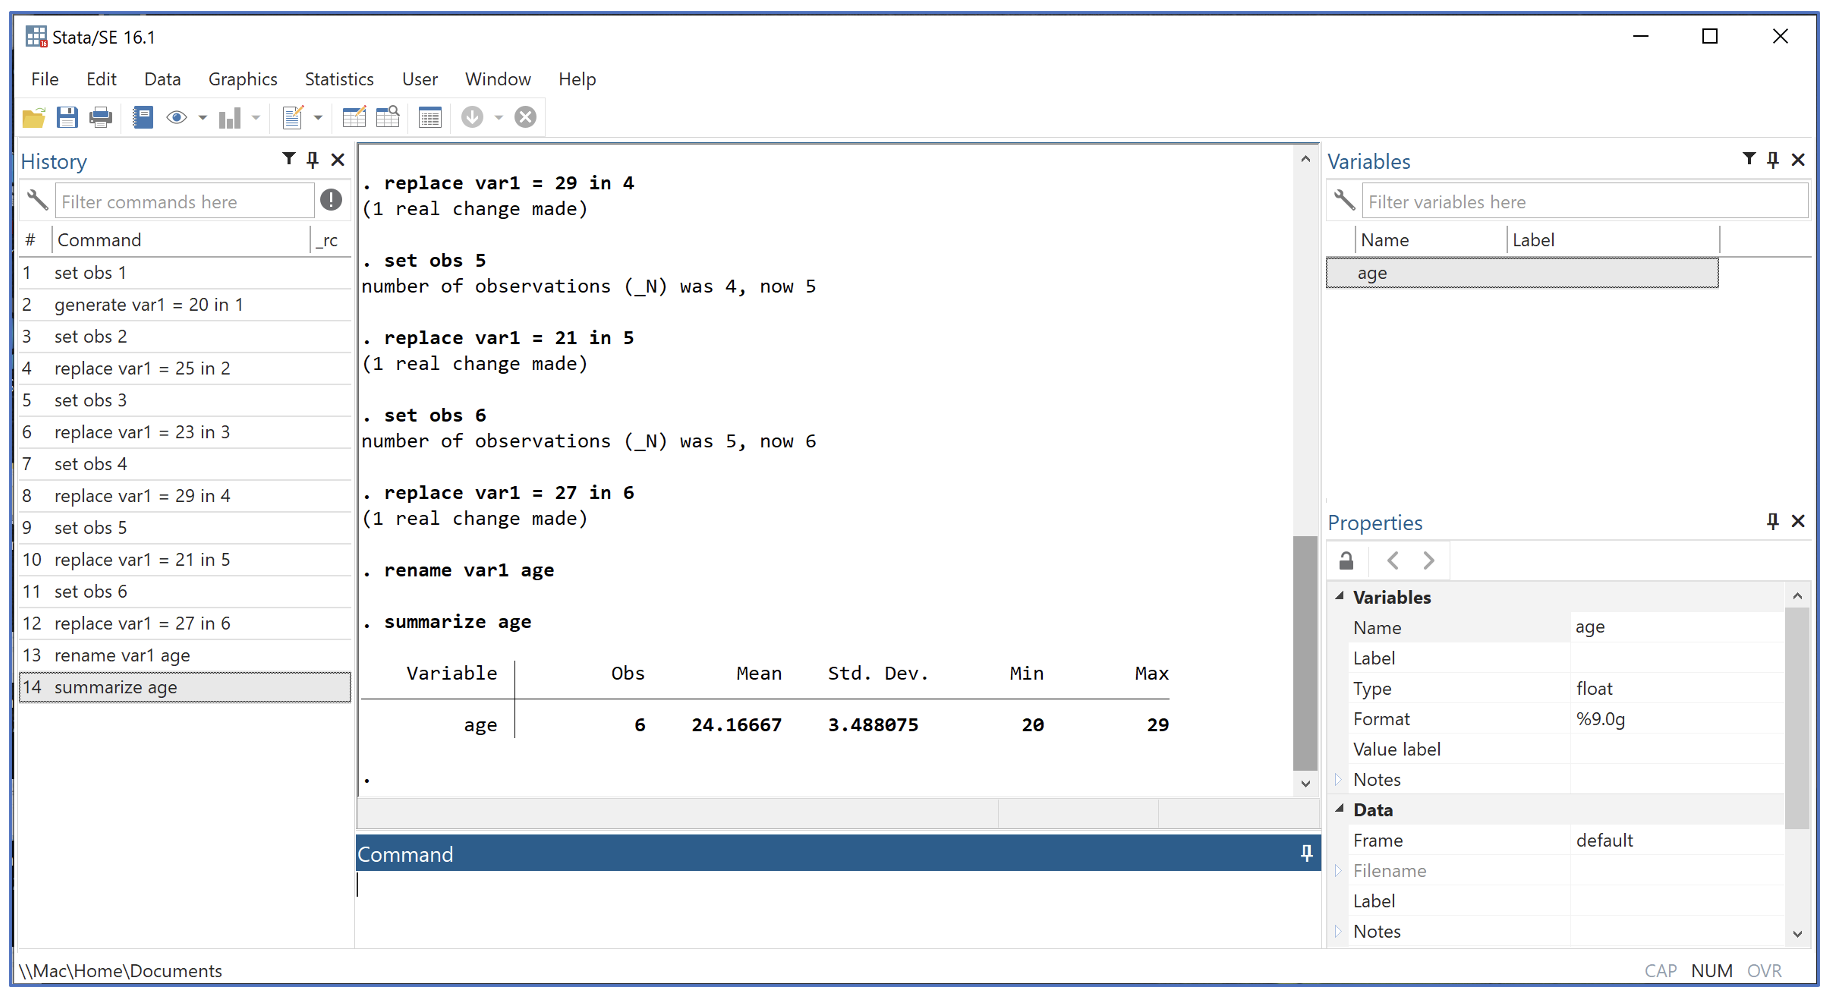
\includegraphics[width=0.75\linewidth]{img/mod01/stata/simple-06}

The final text in the main window provides a summary of \texttt{age}: there are 6 observations, with a mean age of 24.2 years, a standard deviation of 3.49 years, a minimum of 20 and a maximum of 29 years.

\hypertarget{the-stata-environment}{%
\subsection{The Stata environment}\label{the-stata-environment}}

Now that we have seen a simple example of how to use Stata, let's describe the Stata environment. The largest window in Stata is the \textbf{Results} window. This is where the results of your analyses appear, as well as any information, warnings or error messages. You may have noticed that the \textbf{Results} window also contains commands used to conduct analyses. For example, there is a command above summary output for age:

\texttt{.\ summarize\ age}

This command is generated by Stata based on the entries in the \textbf{summarize} dialog box. Stata is inherently a command-driven program: the menus and dialog boxes simply generate commands that Stata interprets, and these commands (and their results) are included in the Results window. While most menu items and dialog boxes can be replicated using commands, it is easier to learn Stata using the menus and dialog boxes. In later Modules, we will include the commands that can be used as alternatives to using the Stata menus.

The Stata windows are summarised below.

\begin{longtable}[]{@{}
  >{\raggedright\arraybackslash}p{(\columnwidth - 2\tabcolsep) * \real{0.5000}}
  >{\raggedright\arraybackslash}p{(\columnwidth - 2\tabcolsep) * \real{0.5000}}@{}}
\toprule()
\begin{minipage}[b]{\linewidth}\raggedright
Window
\end{minipage} & \begin{minipage}[b]{\linewidth}\raggedright
Purpose
\end{minipage} \\
\midrule()
\endhead
Results & Shows your issued commands, results output (e.g.~tables) and error messages or warnings. \\
Command & Where you can type in a command you want to run. The command window need not be used in this course \\
Variables & Gives a list of the variables in your currently opened dataset. \\
Properties & Shows the properties of your currently selected variable (selected from the Variables window) and of your currently opened dataset. \\
History & Shows the history of your issued commands in your current session. \\
Data Editor (Edit) & A separate window that allows you to edit or enter data. \\
Data Editor (Browse) & A separate window that allows you to view data: data cannot be edited. \\
\bottomrule()
\end{longtable}

Stata allows you to perform most of your work by selecting options from the appropriate menus at the top of the main Stata window. A brief description of the main menu bar options follows.

\textbf{File} includes all the options you typically use in other programs, such as Open, Save, Exit. Note, that you can open or create various types of new files. The main type of file we open or create in this course is a Stata data file (.dta). In the Advanced Biostatistics and Statistical Computing course (PHCM9517), we will also use other file types such as a .do file for scripting (or writing) Stata commands.

\textbf{Edit} includes the typical Copy, and Paste commands.

\textbf{Data} allows you to open the \textbf{Data Editor}. You can also create new variables and change current variables using \textbf{Data \textgreater{} Create or change data}.

\textbf{Graphics} includes the commands to create various types of graphs including box plots, histograms, scatterplots, line graphs, and bar charts.

\textbf{Statistics} includes all the commands to carry out statistical analyses and perform power and sample size calculations. Much of this course will focus on using commands located in this menu.

\textbf{User} is for saved files from other windows (e.g.~saved graphs). You will not need to use this option in this course.

\textbf{Window} can be used to select which window you want to view (e.g.~Results, Data Editor).

\textbf{Help} has many useful options including the viewing the PDF documentation, a Search function and other resources for using Stata. We will also demonstrate how to use helpful resources later in this introductory manual. Another useful Stata resource is the video tutorials produced by Stata: \url{https://www.stata.com/links/video-tutorials/}

\hypertarget{part-2-obtaining-basic-descriptive-statistics}{%
\section*{Part 2: Obtaining basic descriptive statistics}\label{part-2-obtaining-basic-descriptive-statistics}}
\addcontentsline{toc}{section}{Part 2: Obtaining basic descriptive statistics}

In this exercise, we will analyse data to complete a descriptive table from a research study. The data come from a study in primary biliary cirrhosis, a condition of the liver, from \citet{therneau_grambsch10}, Modeling Survival Data: Extending the Cox Model. By the end of this exercise, we will have completed the following table.

 
  \providecommand{\huxb}[2]{\arrayrulecolor[RGB]{#1}\global\arrayrulewidth=#2pt}
  \providecommand{\huxvb}[2]{\color[RGB]{#1}\vrule width #2pt}
  \providecommand{\huxtpad}[1]{\rule{0pt}{#1}}
  \providecommand{\huxbpad}[1]{\rule[-#1]{0pt}{#1}}

\begin{table}[ht]
\begin{centerbox}
\begin{threeparttable}
\captionsetup{justification=centering,singlelinecheck=off}
\caption{\label{tab:unnamed-chunk-8} Summary of 418 participants from the PBC study (Therneau and Grambsch, 2000)}
 \setlength{\tabcolsep}{0pt}
\begin{tabularx}{0.95\textwidth}{p{0.316666666666667\textwidth} p{0.316666666666667\textwidth} p{0.316666666666667\textwidth}}


\hhline{>{\huxb{0, 0, 0}{0.4}}->{\huxb{0, 0, 0}{0.4}}->{\huxb{0, 0, 0}{0.4}}-}
\arrayrulecolor{black}

\multicolumn{1}{!{\huxvb{0, 0, 0}{0}}p{0.316666666666667\textwidth}!{\huxvb{0, 0, 0}{0}}}{\hspace{0pt}\parbox[b]{0.316666666666667\textwidth-0pt-6pt}{\huxtpad{6pt + 1em}\raggedright \textbf{Characteristic}\huxbpad{6pt}}} &
\multicolumn{1}{p{0.316666666666667\textwidth}!{\huxvb{0, 0, 0}{0}}}{\hspace{6pt}\parbox[b]{0.316666666666667\textwidth-6pt-6pt}{\huxtpad{6pt + 1em}\raggedright \textbf{ }\huxbpad{6pt}}} &
\multicolumn{1}{p{0.316666666666667\textwidth}!{\huxvb{0, 0, 0}{0}}}{\hspace{6pt}\parbox[b]{0.316666666666667\textwidth-6pt-0pt}{\huxtpad{6pt + 1em}\raggedright \textbf{Summary}\huxbpad{6pt}}} \tabularnewline[-0.5pt]


\hhline{>{\huxb{0, 0, 0}{0.4}}->{\huxb{0, 0, 0}{0.4}}->{\huxb{0, 0, 0}{0.4}}-}
\arrayrulecolor{black}

\multicolumn{1}{!{\huxvb{0, 0, 0}{0}}p{0.316666666666667\textwidth}!{\huxvb{0, 0, 0}{0}}}{\hspace{0pt}\parbox[b]{0.316666666666667\textwidth-0pt-6pt}{\huxtpad{6pt + 1em}\raggedright Age (years)\huxbpad{6pt}}} &
\multicolumn{1}{p{0.316666666666667\textwidth}!{\huxvb{0, 0, 0}{0}}}{\hspace{6pt}\parbox[b]{0.316666666666667\textwidth-6pt-6pt}{\huxtpad{6pt + 1em}\raggedright \huxbpad{6pt}}} &
\multicolumn{1}{p{0.316666666666667\textwidth}!{\huxvb{0, 0, 0}{0}}}{\hspace{6pt}\parbox[b]{0.316666666666667\textwidth-6pt-0pt}{\huxtpad{6pt + 1em}\raggedright Mean (SD) or Median [IQR]\huxbpad{6pt}}} \tabularnewline[-0.5pt]


\hhline{}
\arrayrulecolor{black}

\multicolumn{1}{!{\huxvb{0, 0, 0}{0}}p{0.316666666666667\textwidth}!{\huxvb{0, 0, 0}{0}}}{} &
\multicolumn{1}{p{0.316666666666667\textwidth}!{\huxvb{0, 0, 0}{0}}}{\hspace{6pt}\parbox[b]{0.316666666666667\textwidth-6pt-6pt}{\huxtpad{6pt + 1em}\raggedright Male\huxbpad{6pt}}} &
\multicolumn{1}{p{0.316666666666667\textwidth}!{\huxvb{0, 0, 0}{0}}}{\hspace{6pt}\parbox[b]{0.316666666666667\textwidth-6pt-0pt}{\huxtpad{6pt + 1em}\raggedright n (\%)\huxbpad{6pt}}} \tabularnewline[-0.5pt]


\hhline{}
\arrayrulecolor{black}

\multicolumn{1}{!{\huxvb{0, 0, 0}{0}}p{0.316666666666667\textwidth}!{\huxvb{0, 0, 0}{0}}}{\multirow[t]{-2}{*}[0ex]{\hspace{0pt}\parbox[b]{0.316666666666667\textwidth-0pt-6pt}{\huxtpad{6pt + 1em}\raggedright Sex\huxbpad{6pt}}}} &
\multicolumn{1}{p{0.316666666666667\textwidth}!{\huxvb{0, 0, 0}{0}}}{\hspace{6pt}\parbox[b]{0.316666666666667\textwidth-6pt-6pt}{\huxtpad{6pt + 1em}\raggedright Female\huxbpad{6pt}}} &
\multicolumn{1}{p{0.316666666666667\textwidth}!{\huxvb{0, 0, 0}{0}}}{\hspace{6pt}\parbox[b]{0.316666666666667\textwidth-6pt-0pt}{\huxtpad{6pt + 1em}\raggedright n (\%)\huxbpad{6pt}}} \tabularnewline[-0.5pt]


\hhline{}
\arrayrulecolor{black}

\multicolumn{1}{!{\huxvb{0, 0, 0}{0}}p{0.316666666666667\textwidth}!{\huxvb{0, 0, 0}{0}}}{\hspace{0pt}\parbox[b]{0.316666666666667\textwidth-0pt-6pt}{\huxtpad{6pt + 1em}\raggedright AST* (U/ml)\huxbpad{6pt}}} &
\multicolumn{1}{p{0.316666666666667\textwidth}!{\huxvb{0, 0, 0}{0}}}{\hspace{6pt}\parbox[b]{0.316666666666667\textwidth-6pt-6pt}{\huxtpad{6pt + 1em}\raggedright \huxbpad{6pt}}} &
\multicolumn{1}{p{0.316666666666667\textwidth}!{\huxvb{0, 0, 0}{0}}}{\hspace{6pt}\parbox[b]{0.316666666666667\textwidth-6pt-0pt}{\huxtpad{6pt + 1em}\raggedright Mean (SD) or Median [IQR]\huxbpad{6pt}}} \tabularnewline[-0.5pt]


\hhline{}
\arrayrulecolor{black}

\multicolumn{1}{!{\huxvb{0, 0, 0}{0}}p{0.316666666666667\textwidth}!{\huxvb{0, 0, 0}{0}}}{\hspace{0pt}\parbox[b]{0.316666666666667\textwidth-0pt-6pt}{\huxtpad{6pt + 1em}\raggedright Serum bilirubin\huxbpad{6pt}}} &
\multicolumn{1}{p{0.316666666666667\textwidth}!{\huxvb{0, 0, 0}{0}}}{\hspace{6pt}\parbox[b]{0.316666666666667\textwidth-6pt-6pt}{\huxtpad{6pt + 1em}\raggedright \huxbpad{6pt}}} &
\multicolumn{1}{p{0.316666666666667\textwidth}!{\huxvb{0, 0, 0}{0}}}{\hspace{6pt}\parbox[b]{0.316666666666667\textwidth-6pt-0pt}{\huxtpad{6pt + 1em}\raggedright Mean (SD) or Median [IQR]\huxbpad{6pt}}} \tabularnewline[-0.5pt]


\hhline{}
\arrayrulecolor{black}

\multicolumn{1}{!{\huxvb{0, 0, 0}{0}}p{0.316666666666667\textwidth}!{\huxvb{0, 0, 0}{0}}}{} &
\multicolumn{1}{p{0.316666666666667\textwidth}!{\huxvb{0, 0, 0}{0}}}{\hspace{6pt}\parbox[b]{0.316666666666667\textwidth-6pt-6pt}{\huxtpad{6pt + 1em}\raggedright I\huxbpad{6pt}}} &
\multicolumn{1}{p{0.316666666666667\textwidth}!{\huxvb{0, 0, 0}{0}}}{\hspace{6pt}\parbox[b]{0.316666666666667\textwidth-6pt-0pt}{\huxtpad{6pt + 1em}\raggedright n (\%)\huxbpad{6pt}}} \tabularnewline[-0.5pt]


\hhline{}
\arrayrulecolor{black}

\multicolumn{1}{!{\huxvb{0, 0, 0}{0}}p{0.316666666666667\textwidth}!{\huxvb{0, 0, 0}{0}}}{} &
\multicolumn{1}{p{0.316666666666667\textwidth}!{\huxvb{0, 0, 0}{0}}}{\hspace{6pt}\parbox[b]{0.316666666666667\textwidth-6pt-6pt}{\huxtpad{6pt + 1em}\raggedright II\huxbpad{6pt}}} &
\multicolumn{1}{p{0.316666666666667\textwidth}!{\huxvb{0, 0, 0}{0}}}{\hspace{6pt}\parbox[b]{0.316666666666667\textwidth-6pt-0pt}{\huxtpad{6pt + 1em}\raggedright n (\%)\huxbpad{6pt}}} \tabularnewline[-0.5pt]


\hhline{}
\arrayrulecolor{black}

\multicolumn{1}{!{\huxvb{0, 0, 0}{0}}p{0.316666666666667\textwidth}!{\huxvb{0, 0, 0}{0}}}{} &
\multicolumn{1}{p{0.316666666666667\textwidth}!{\huxvb{0, 0, 0}{0}}}{\hspace{6pt}\parbox[b]{0.316666666666667\textwidth-6pt-6pt}{\huxtpad{6pt + 1em}\raggedright III\huxbpad{6pt}}} &
\multicolumn{1}{p{0.316666666666667\textwidth}!{\huxvb{0, 0, 0}{0}}}{\hspace{6pt}\parbox[b]{0.316666666666667\textwidth-6pt-0pt}{\huxtpad{6pt + 1em}\raggedright n (\%)\huxbpad{6pt}}} \tabularnewline[-0.5pt]


\hhline{}
\arrayrulecolor{black}

\multicolumn{1}{!{\huxvb{0, 0, 0}{0}}p{0.316666666666667\textwidth}!{\huxvb{0, 0, 0}{0}}}{\multirow[t]{-4}{*}[0ex]{\hspace{0pt}\parbox[b]{0.316666666666667\textwidth-0pt-6pt}{\huxtpad{6pt + 1em}\raggedright Stage\huxbpad{6pt}}}} &
\multicolumn{1}{p{0.316666666666667\textwidth}!{\huxvb{0, 0, 0}{0}}}{\hspace{6pt}\parbox[b]{0.316666666666667\textwidth-6pt-6pt}{\huxtpad{6pt + 1em}\raggedright IIIV\huxbpad{6pt}}} &
\multicolumn{1}{p{0.316666666666667\textwidth}!{\huxvb{0, 0, 0}{0}}}{\hspace{6pt}\parbox[b]{0.316666666666667\textwidth-6pt-0pt}{\huxtpad{6pt + 1em}\raggedright n (\%)\huxbpad{6pt}}} \tabularnewline[-0.5pt]


\hhline{}
\arrayrulecolor{black}

\multicolumn{1}{!{\huxvb{0, 0, 0}{0}}p{0.316666666666667\textwidth}!{\huxvb{0, 0, 0}{0}}}{} &
\multicolumn{1}{p{0.316666666666667\textwidth}!{\huxvb{0, 0, 0}{0}}}{\hspace{6pt}\parbox[b]{0.316666666666667\textwidth-6pt-6pt}{\huxtpad{6pt + 1em}\raggedright Alive: no transplant\huxbpad{6pt}}} &
\multicolumn{1}{p{0.316666666666667\textwidth}!{\huxvb{0, 0, 0}{0}}}{\hspace{6pt}\parbox[b]{0.316666666666667\textwidth-6pt-0pt}{\huxtpad{6pt + 1em}\raggedright n (\%)\huxbpad{6pt}}} \tabularnewline[-0.5pt]


\hhline{}
\arrayrulecolor{black}

\multicolumn{1}{!{\huxvb{0, 0, 0}{0}}p{0.316666666666667\textwidth}!{\huxvb{0, 0, 0}{0}}}{} &
\multicolumn{1}{p{0.316666666666667\textwidth}!{\huxvb{0, 0, 0}{0}}}{\hspace{6pt}\parbox[b]{0.316666666666667\textwidth-6pt-6pt}{\huxtpad{6pt + 1em}\raggedright Alive: transplant\huxbpad{6pt}}} &
\multicolumn{1}{p{0.316666666666667\textwidth}!{\huxvb{0, 0, 0}{0}}}{\hspace{6pt}\parbox[b]{0.316666666666667\textwidth-6pt-0pt}{\huxtpad{6pt + 1em}\raggedright n (\%)\huxbpad{6pt}}} \tabularnewline[-0.5pt]


\hhline{}
\arrayrulecolor{black}

\multicolumn{1}{!{\huxvb{0, 0, 0}{0}}p{0.316666666666667\textwidth}!{\huxvb{0, 0, 0}{0}}}{\multirow[t]{-3}{*}[0ex]{\hspace{0pt}\parbox[b]{0.316666666666667\textwidth-0pt-6pt}{\huxtpad{6pt + 1em}\raggedright Vital status at study end\huxbpad{6pt}}}} &
\multicolumn{1}{p{0.316666666666667\textwidth}!{\huxvb{0, 0, 0}{0}}}{\hspace{6pt}\parbox[b]{0.316666666666667\textwidth-6pt-6pt}{\huxtpad{6pt + 1em}\raggedright Deceased\huxbpad{6pt}}} &
\multicolumn{1}{p{0.316666666666667\textwidth}!{\huxvb{0, 0, 0}{0}}}{\hspace{6pt}\parbox[b]{0.316666666666667\textwidth-6pt-0pt}{\huxtpad{6pt + 1em}\raggedright n (\%)\huxbpad{6pt}}} \tabularnewline[-0.5pt]


\hhline{>{\huxb{0, 0, 0}{0.8}}->{\huxb{0, 0, 0}{0.8}}->{\huxb{0, 0, 0}{0.8}}-}
\arrayrulecolor{black}

\multicolumn{3}{!{\huxvb{0, 0, 0}{0}}p{0.95\textwidth+4\tabcolsep}!{\huxvb{0, 0, 0}{0}}}{\hspace{6pt}\parbox[b]{0.95\textwidth+4\tabcolsep-6pt-6pt}{\huxtpad{6pt + 1em}\raggedright * asparate aminotransferase\huxbpad{6pt}}} \tabularnewline[-0.5pt]


\hhline{}
\arrayrulecolor{black}
\end{tabularx}
\end{threeparttable}\par\end{centerbox}

\end{table}
 

This table is available in Table1.docx, saved on Moodle.

\hypertarget{opening-a-stata-data-file}{%
\subsection{Opening a Stata data file}\label{opening-a-stata-data-file}}

Typing data directly into Stata is not common; we usually open data that have been saved as a Stata data file, or import data that have been entered into another package. Here, we will open a dataset that has been stored as a Stata data file (which has the \texttt{.dta} suffix).

\begin{enumerate}
\def\labelenumi{\arabic{enumi}.}
\tightlist
\item
  Locate the data set called \texttt{pbc.dta} on Moodle. Click the file to download it, and then save it in a folder you will be able to locate later - for example, your OneDrive folder. The description of this dataset (i.e.~the metadata) have been saved as a plain text file: \texttt{pbc\_info.txt}
\item
  In Stata, choose \textbf{File \textgreater{} Open}. Browse to where you stored the dataset and click \textbf{Open}.
\item
  You may get an error: ``Data in memory have changed''. This means that you have not saved a copy of your current data, and by importing a new dataset, your changes will be lost. As Stata can only open one set of data at a time, you can choose to: Save your current data, Don't Save your current data, or Cancel. We don't need to save the data from our simple analysis (the six ages), so we can choose Don't Save.
\end{enumerate}

After opening the data successfully, there will be 418 rows of data, and 20 variables. Examine the \texttt{pbc\_info.txt} file for a description of each variable.

\hypertarget{assigning-variable-labels}{%
\subsection{Assigning variable labels}\label{assigning-variable-labels}}

As we saw earlier, Stata has specific rules about variable names. Variable labels can be used to obtain more descriptive output. For example, the variable entered as bili can be labelled ``Serum bilirubin (mg/dl)''.

To apply a variable label, open the Variables Manager: \textbf{Data \textgreater{} Variables Manager}. Here we can click the variable to be labelled, and enter the new variable label and click \textbf{Apply}:

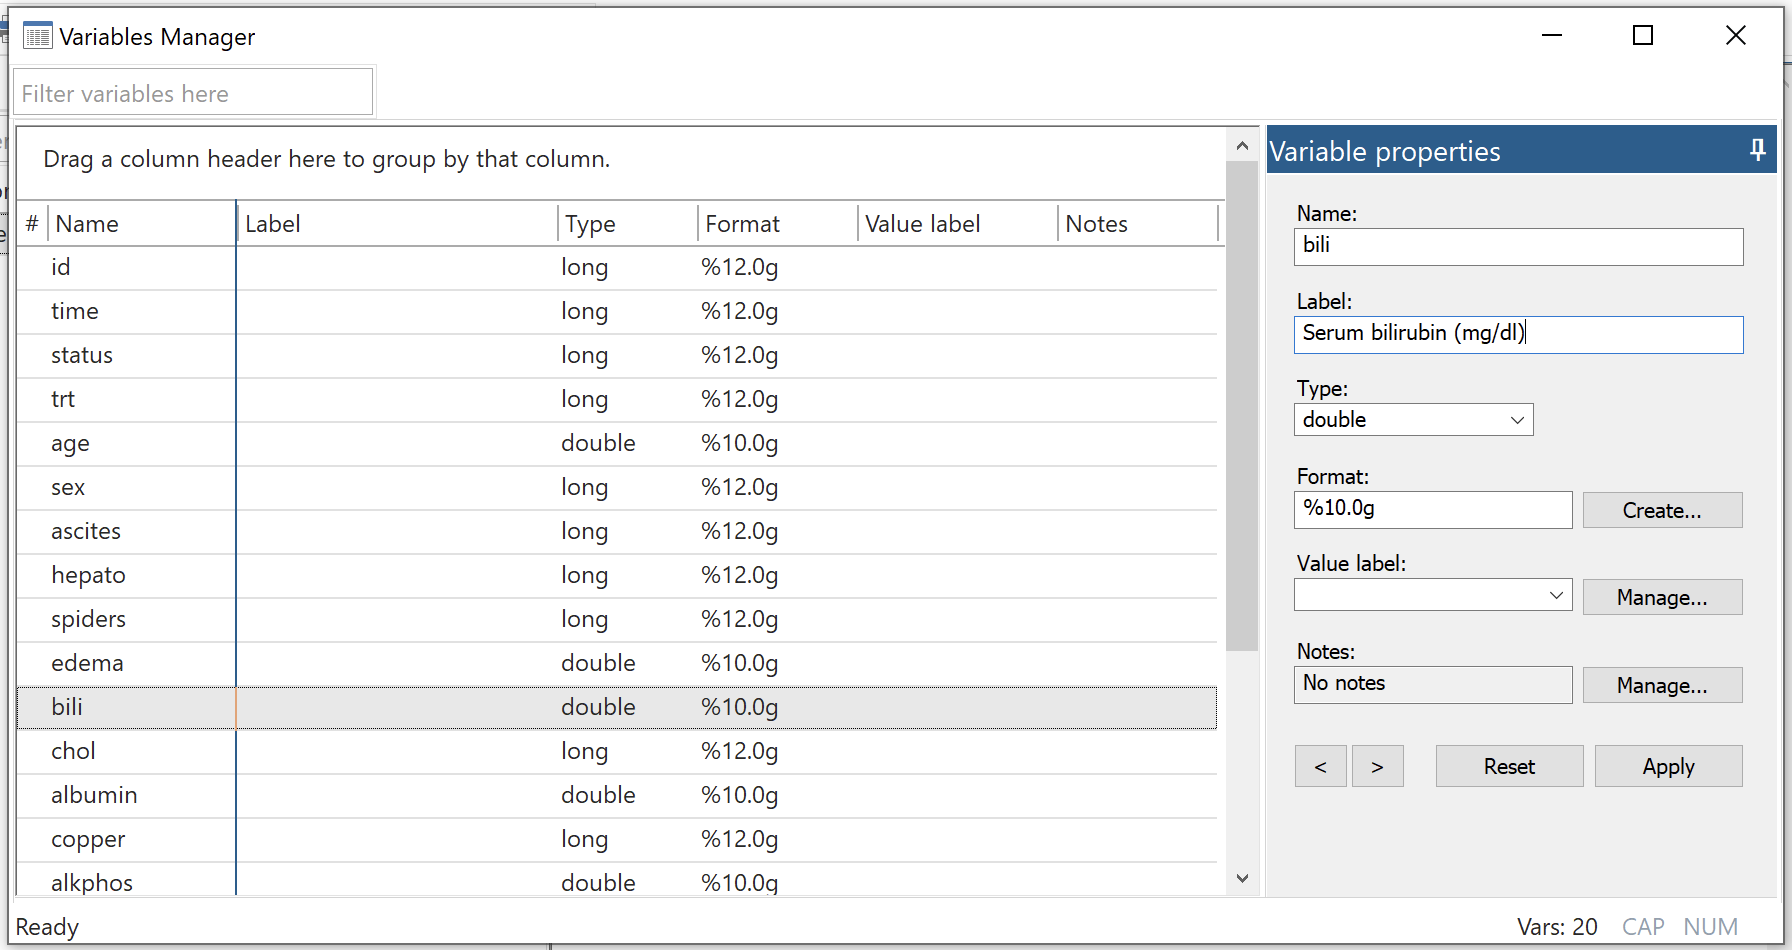
\includegraphics[width=0.75\linewidth]{img/mod01/stata/label-01}

The variable label will now be used in place of the variable name in most output:

\begin{Shaded}
\begin{Highlighting}[]
\NormalTok{. summarize bili, detail}

\NormalTok{                   Serum bilirubin (mg/dl)}
\NormalTok{{-}{-}{-}{-}{-}{-}{-}{-}{-}{-}{-}{-}{-}{-}{-}{-}{-}{-}{-}{-}{-}{-}{-}{-}{-}{-}{-}{-}{-}{-}{-}{-}{-}{-}{-}{-}{-}{-}{-}{-}{-}{-}{-}{-}{-}{-}{-}{-}{-}{-}{-}{-}{-}{-}{-}{-}{-}{-}{-}{-}{-}}
\NormalTok{      Percentiles      Smallest}
\NormalTok{ 1\%           .4             .3}
\NormalTok{ 5\%           .5             .3}
\NormalTok{10\%           .6             .3       Obs                 418}
\NormalTok{25\%           .8             .4       Sum of Wgt.         418}

\NormalTok{50\%          1.4                      Mean           3.220813}
\NormalTok{                        Largest       Std. Dev.      4.407506}
\NormalTok{75\%          3.4           22.5}
\NormalTok{90\%          8.1           24.5       Variance       19.42611}
\NormalTok{95\%           14           25.5       Skewness       2.707849}
\NormalTok{99\%         21.6             28       Kurtosis       10.95486}
\end{Highlighting}
\end{Shaded}

\textbf{TASK:} Assign meaningful variable labels to the variables used in Table 1.

\hypertarget{summarising-continuous-variables}{%
\subsection{Summarising continuous variables}\label{summarising-continuous-variables}}

As we saw in Part 1, continuous variables can be summarised using \textbf{Statistics \textgreater{} Summaries, tables and tests \textgreater{} Summary and descriptive statistics \textgreater{} Summary statistics}. There are three continuous variables that we would like to summarise: age, AST and serum bilirubin. Each of these can be listed in the \textbf{summarize} dialog box, as shown below.

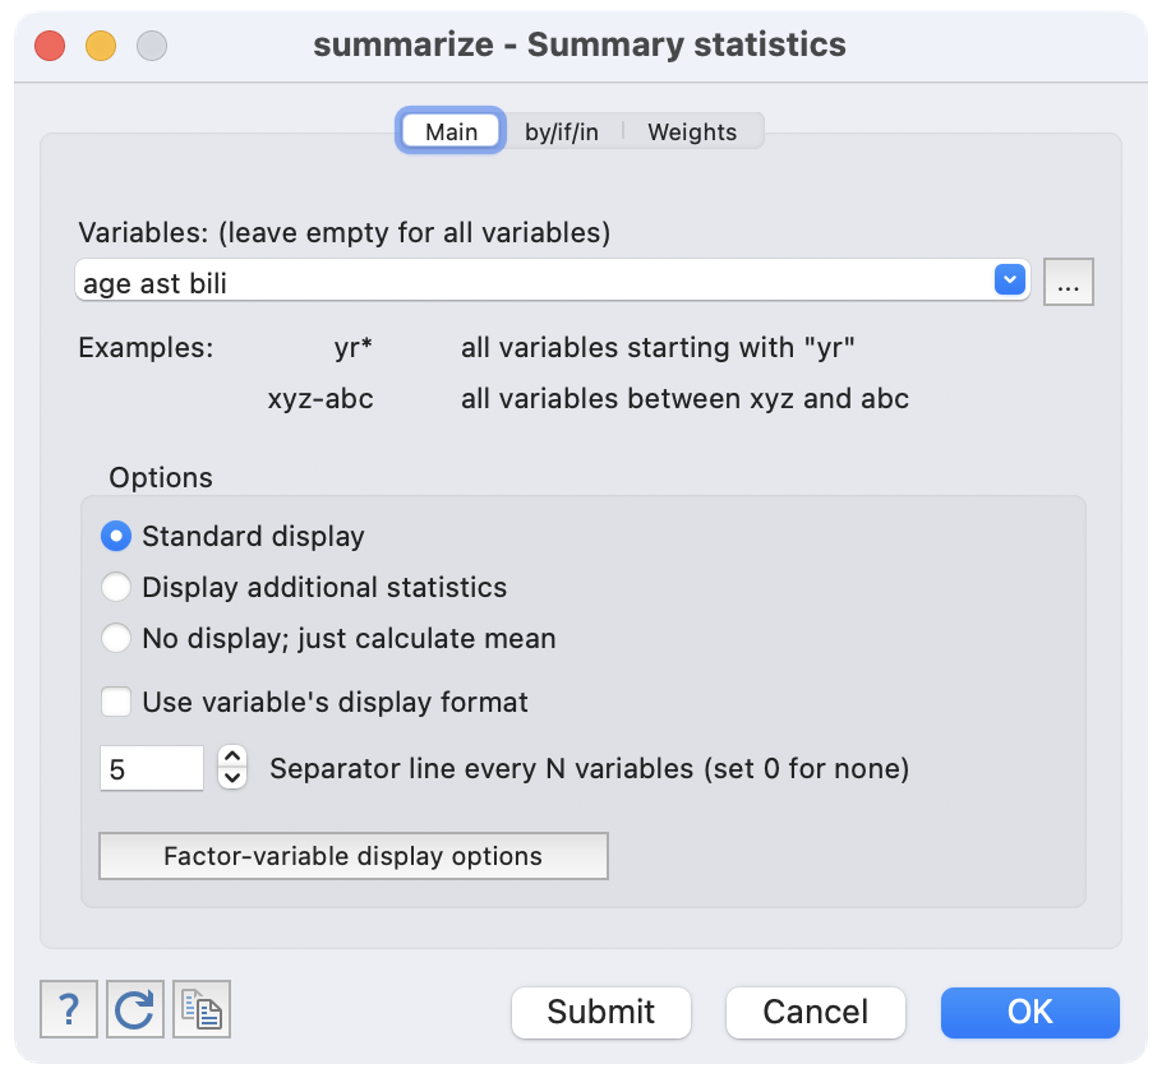
\includegraphics[width=0.75\linewidth]{img/mod01/stata/summ-01}

By default, the summarize command calculates the mean, standard deviation, minimum and maximum. We may be interested in obtaining the median and interquartile ranges, so we select the \textbf{Display additional statistics} option:

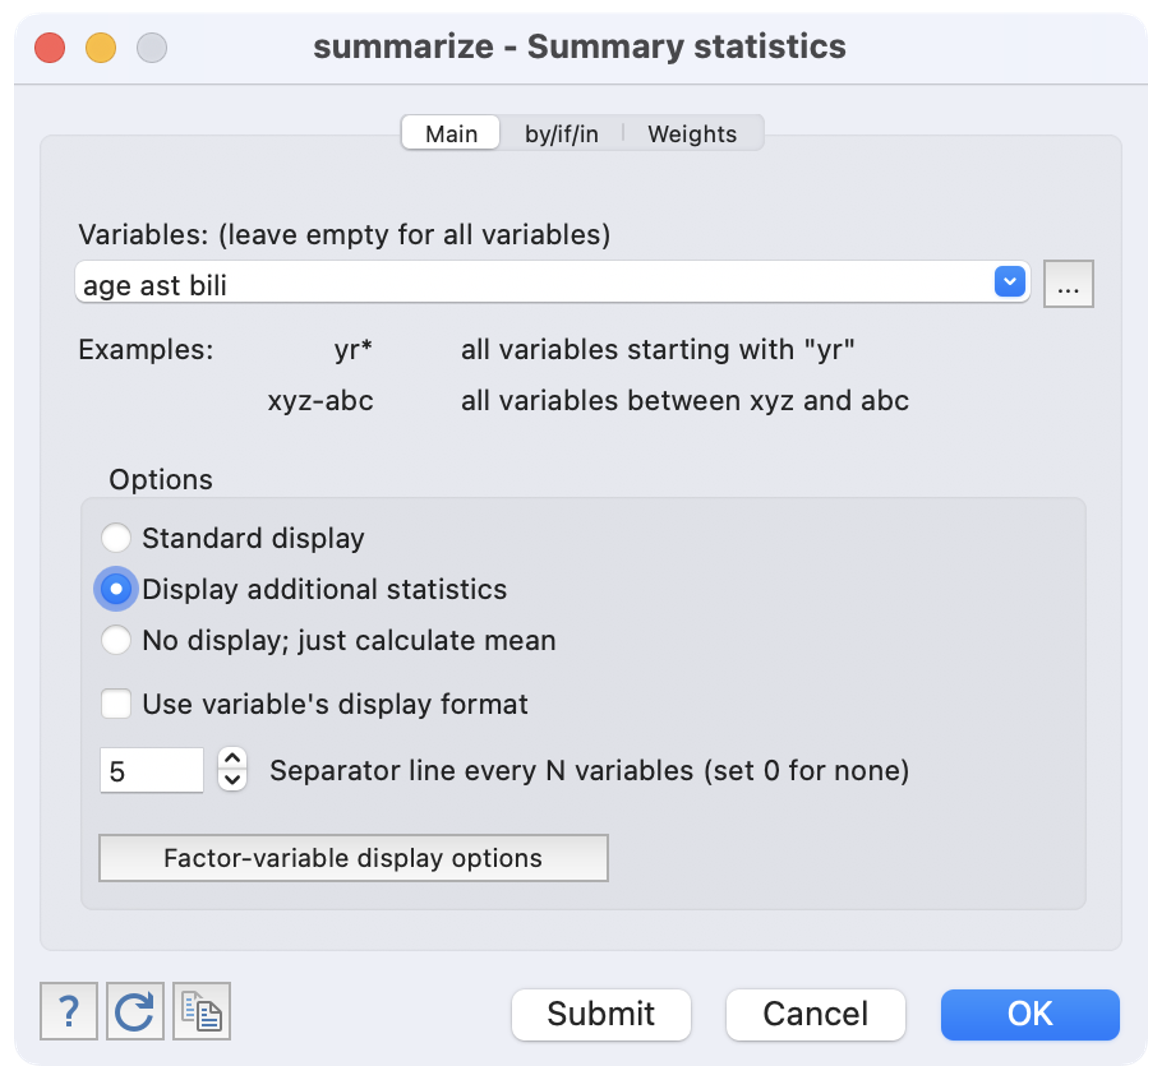
\includegraphics[width=0.75\linewidth]{img/mod01/stata/summ-02}

Summary statistics are produced for each of the three variables. We will use describe the output for age:

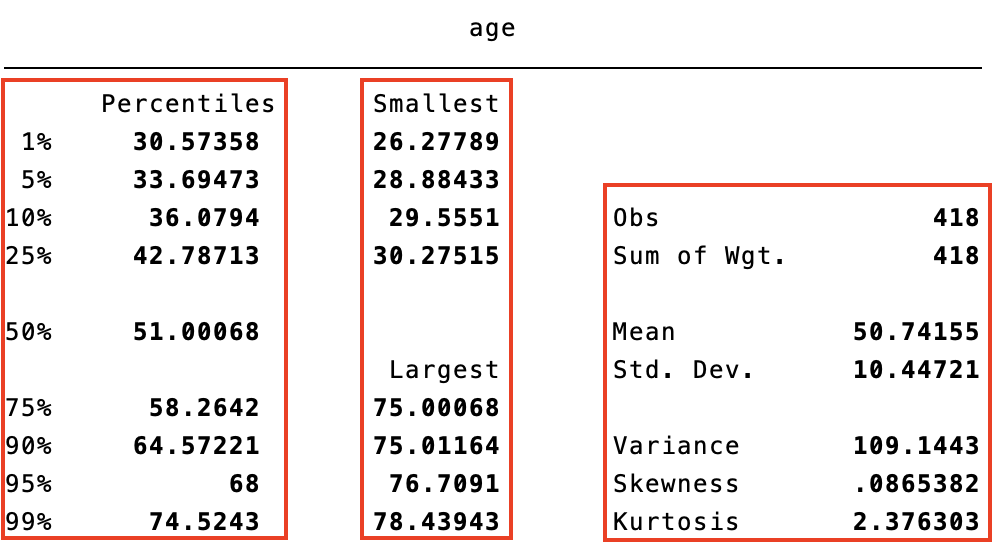
\includegraphics[width=0.75\linewidth]{img/mod01/stata/summ-03}

The output for a detailed summary in Stata should be read as three separate columns. The right-most column lists the number of observations, the mean and standard deviation and other numeric statistics. The left-most column contains the Percentiles: median (50\%), lower quartile (25\%) and upper quartile (75\%). The middle column lists the four smallest and four largest observations, so that we can assess whether the smallest and largest observations are plausible.

For each of our three continuous variables, we need to decide whether to present the mean and standard deviation, or the median and interquartile range. This decision can be made after examining a histogram and boxplot for each variable.

\hypertarget{producing-a-histogram}{%
\subsection{Producing a histogram}\label{producing-a-histogram}}

To produce a histogram, go to menu \textbf{Graphics \textgreater{} Histogram}. Choose the variable to be plotted in the \textbf{Variable} box, and choose the \textbf{Frequency} radio button so that a frequency histogram is produced. Note that only one variable can be plotted at a time, so this procedure will need to be repeated for each continuous variable.

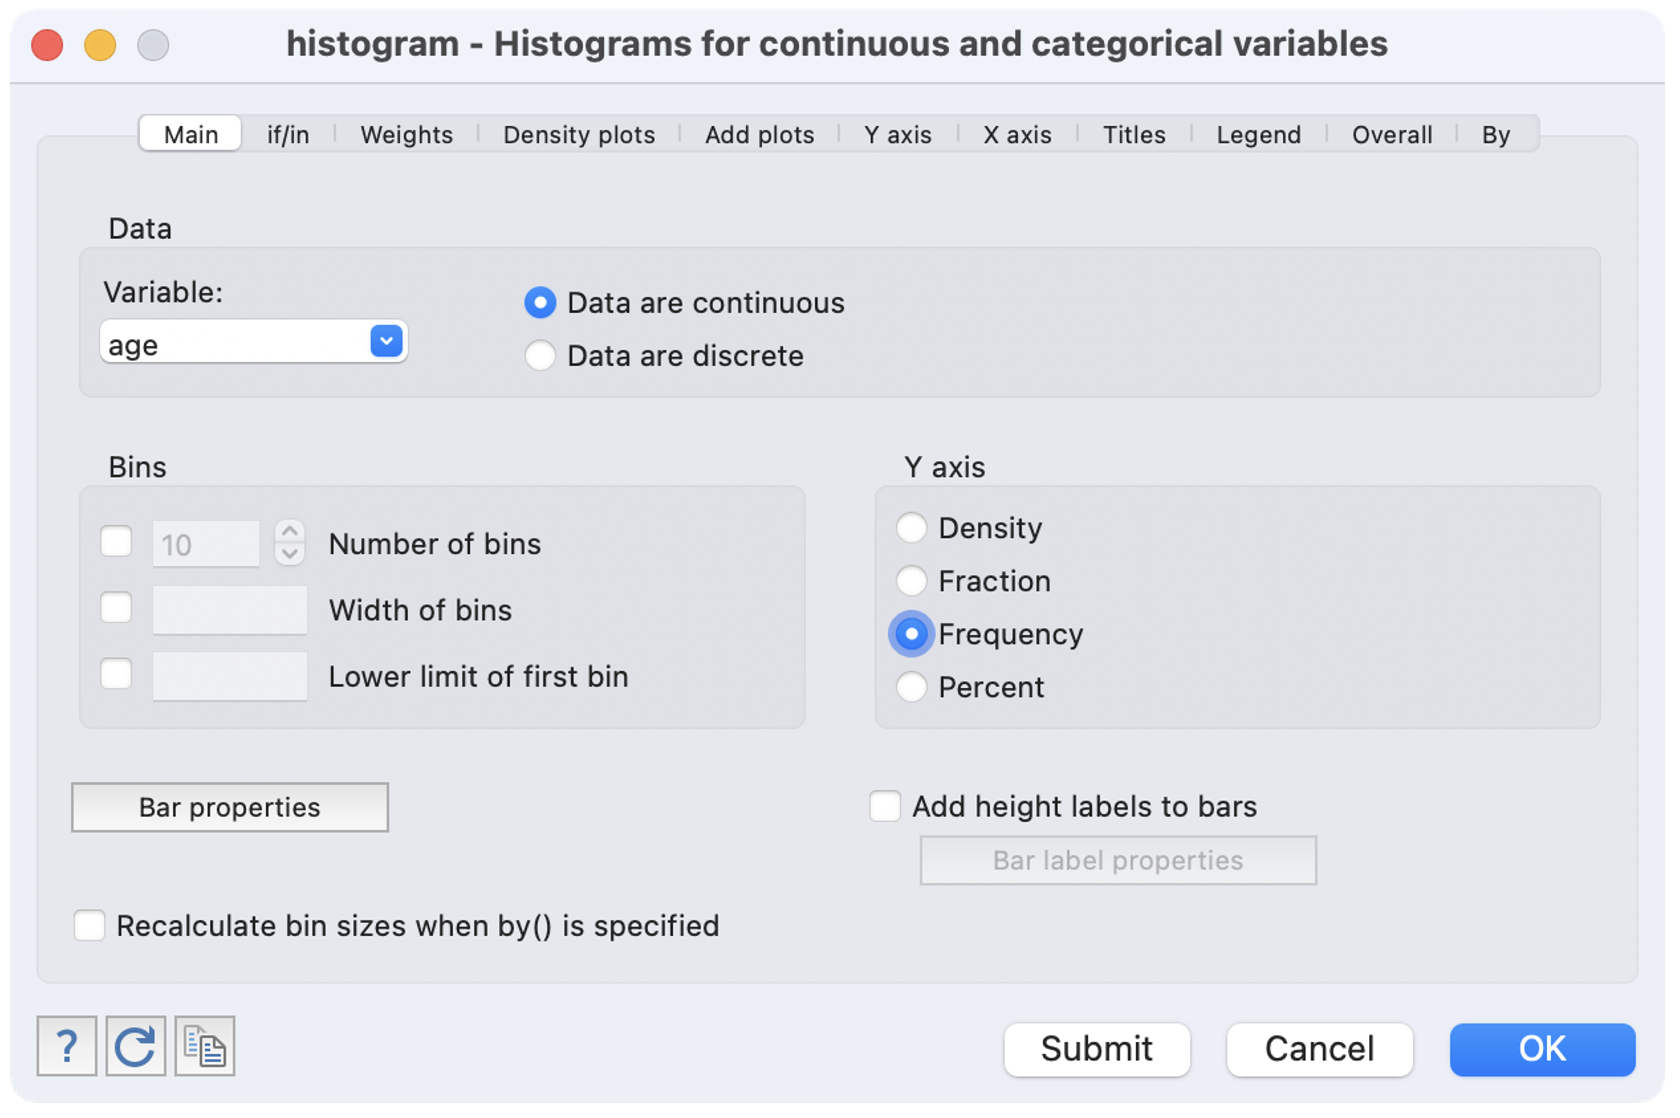
\includegraphics[width=0.75\linewidth]{img/mod01/stata/hist-01}

The default histogram for age appears below.

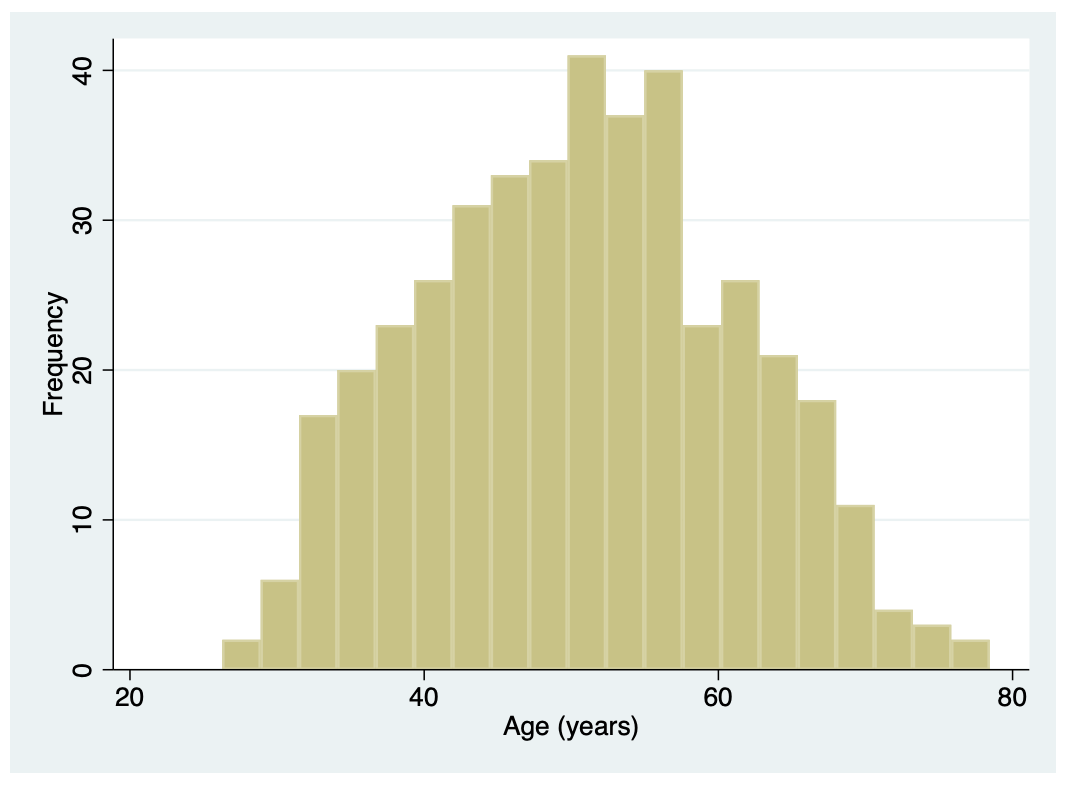
\includegraphics[width=0.75\linewidth]{img/mod01/stata/hist-02}

Stata will automatically choose the number of bins and the width of each bin, however these decisions may not always produce the most optimal histogram. These options can be altered by defining either: the number of bins, or the bin width (but not both); and/or the lower limit of the first bin.

Looking at the command window, Stata has used the following parameters to define the histogram: bin=20, start=26.277892, width=2.6080767. This means that Stata has chosen 20 bins to represent the data, with the first bin starting at 26.2 years and each bin representing 2.6 years. A more easily read histogram might have a bin-width of 5, starting at 25 years of age, so that age categories represent 25 to less than 30, 30 to less than 35 etc, as defined below:

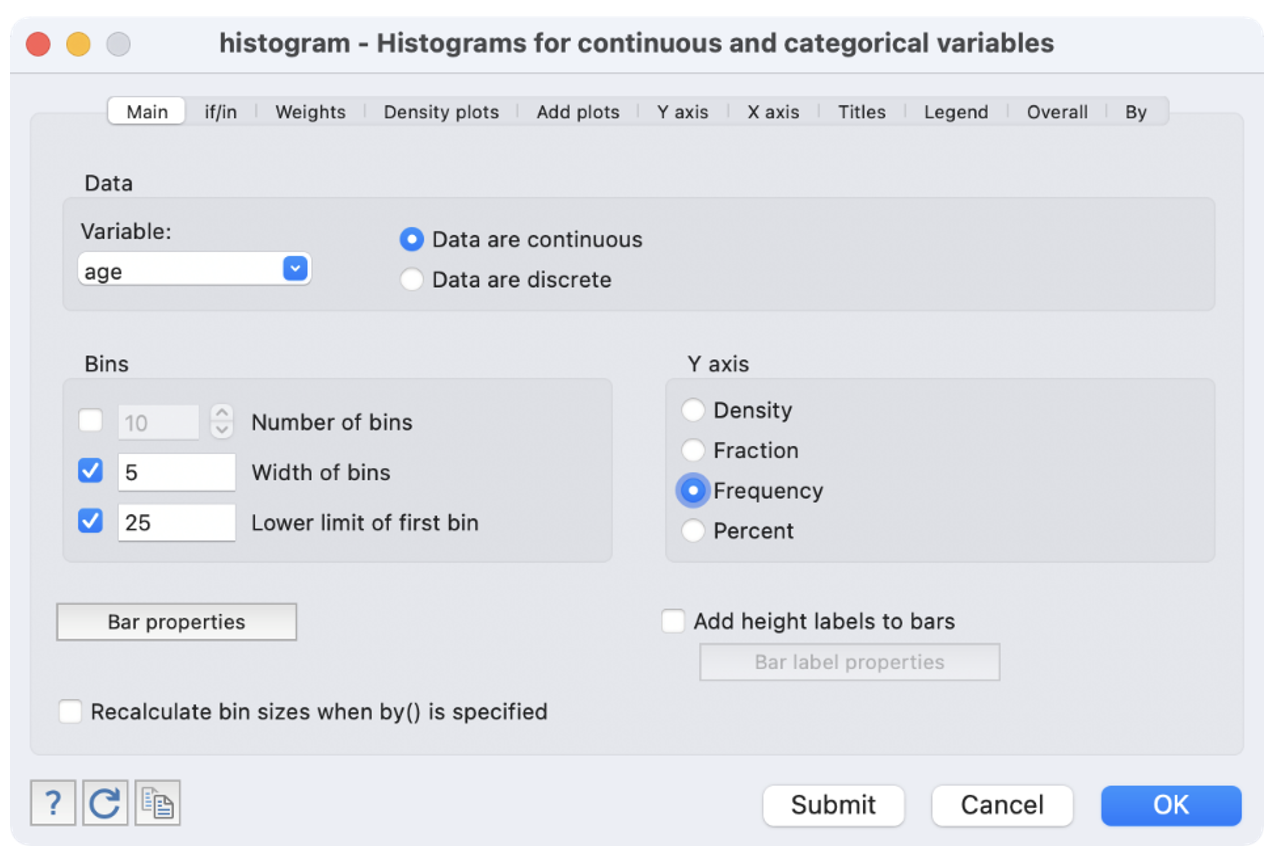
\includegraphics[width=0.75\linewidth]{img/mod01/stata/hist-03}

This results in a histogram with fewer bars and more sensible cut-points:

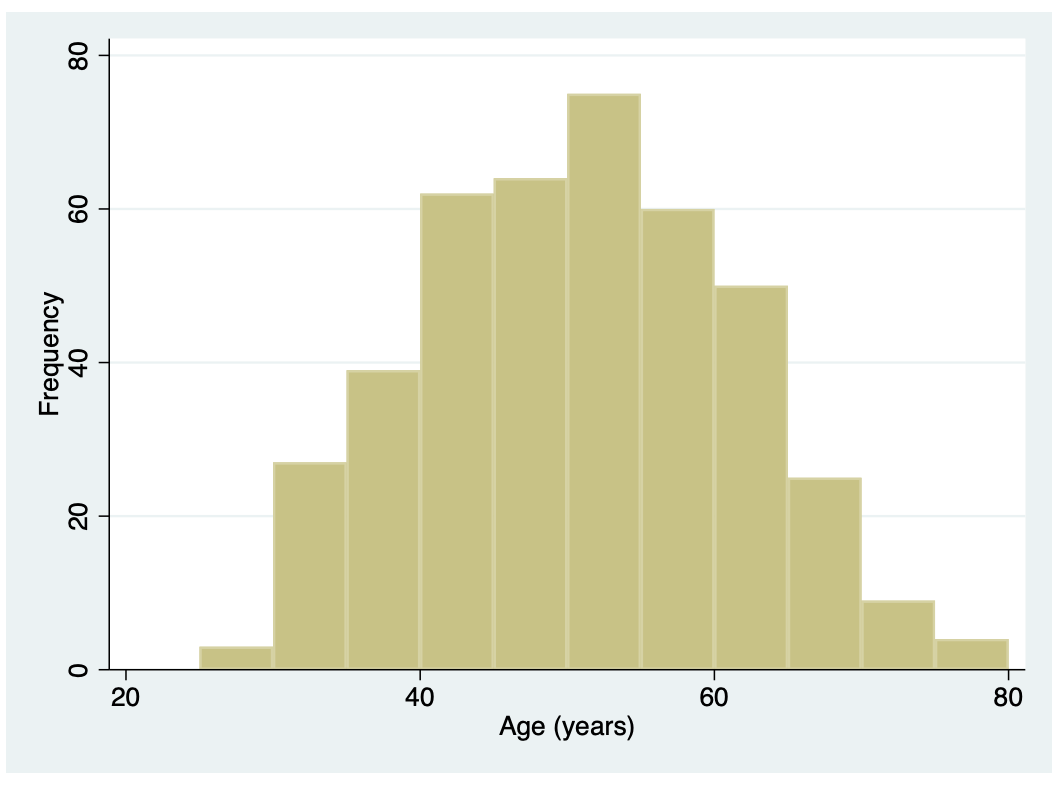
\includegraphics[width=0.75\linewidth]{img/mod01/stata/hist-04}

\hypertarget{producing-a-boxplot}{%
\subsection{Producing a boxplot}\label{producing-a-boxplot}}

The boxplot dialog box is similar to the histogram dialog box. While it is possible to specify more than one variable to be plotted, this is not recommended when variables are measured on very different scales as all variables are plotted on a chart with the same scale.

\textbf{TASK:} Obtain histograms and boxplots for age, AST and bilirubin. Based on these plots, decide whether the mean or the median is the appropriate summary to use for each variable. Transfer your summary statistics to Table 1.

\hypertarget{producing-a-one-way-frequency-table}{%
\subsection{Producing a one-way frequency table}\label{producing-a-one-way-frequency-table}}

We have three categorical variables to summarise in Table 1: sex, stage and vital status. These variables are best summarised using one-way frequency tables.

Choose \textbf{Statistics \textgreater{} Summaries, tables, and tests \textgreater{} Frequency tables \textgreater{} One-way table}. Choose the variable to be summarised as the \textbf{Categorical variable}, and leave all other options unchanged:

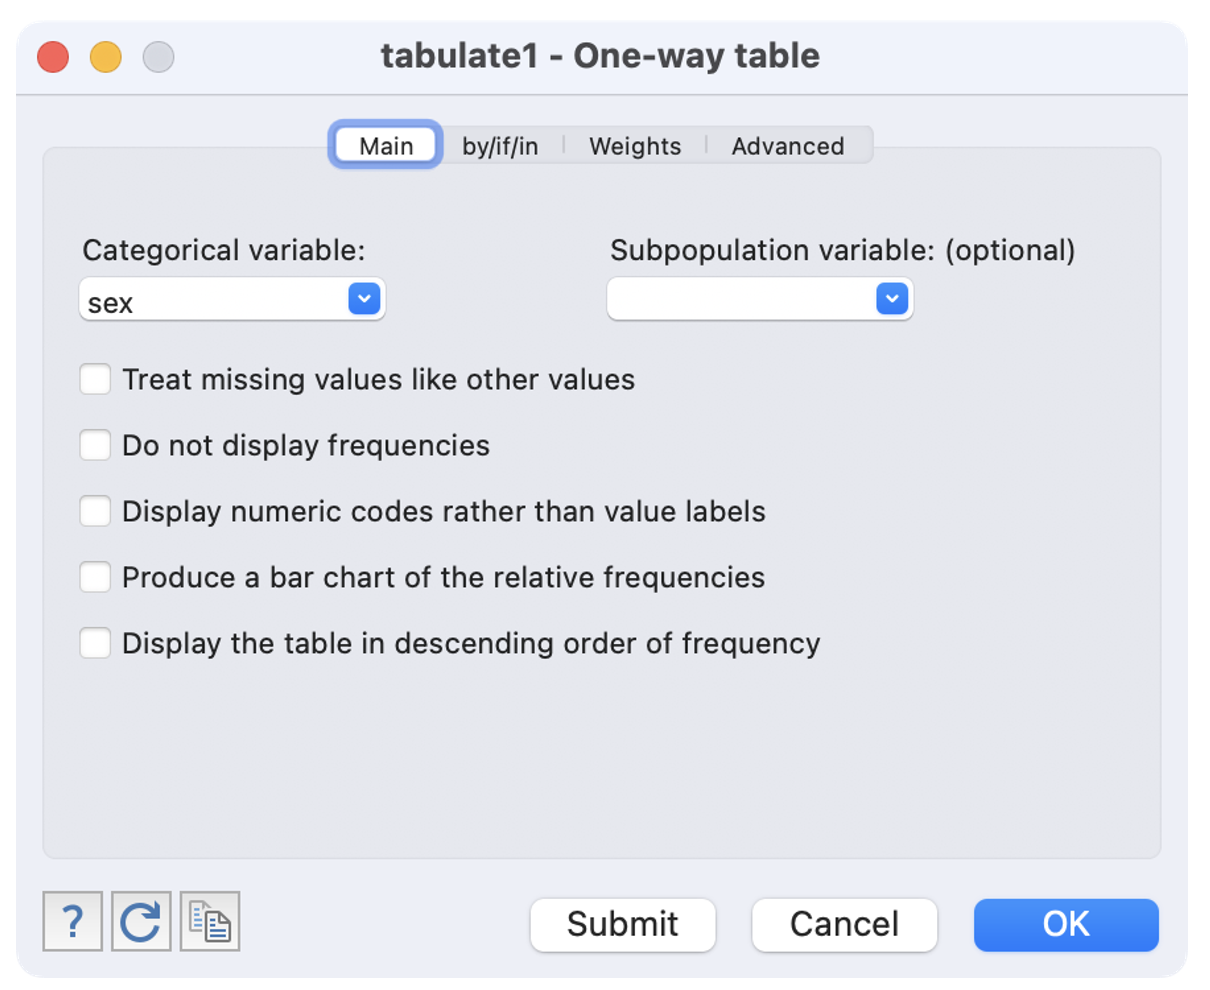
\includegraphics[width=0.75\linewidth]{img/mod01/stata/tab-01}

Click \textbf{OK} to obtain the following table:

\begin{Shaded}
\begin{Highlighting}[]
\NormalTok{        sex |      Freq.     Percent        Cum.}
\NormalTok{{-}{-}{-}{-}{-}{-}{-}{-}{-}{-}{-}{-}+{-}{-}{-}{-}{-}{-}{-}{-}{-}{-}{-}{-}{-}{-}{-}{-}{-}{-}{-}{-}{-}{-}{-}{-}{-}{-}{-}{-}{-}{-}{-}{-}{-}{-}{-}}
\NormalTok{          1 |         44       10.53       10.53}
\NormalTok{          2 |        374       89.47      100.00}
\NormalTok{{-}{-}{-}{-}{-}{-}{-}{-}{-}{-}{-}{-}+{-}{-}{-}{-}{-}{-}{-}{-}{-}{-}{-}{-}{-}{-}{-}{-}{-}{-}{-}{-}{-}{-}{-}{-}{-}{-}{-}{-}{-}{-}{-}{-}{-}{-}{-}}
\NormalTok{      Total |        418      100.00}
\end{Highlighting}
\end{Shaded}

\hypertarget{assigning-value-labels-to-categorical-variables}{%
\subsection{Assigning value labels to categorical variables}\label{assigning-value-labels-to-categorical-variables}}

You will notice that the table above, in its current form, is uninterpretable as the 1 and 2 categories are not labelled. In this course, all variables including categorical variables are numerically coded. This is because ``string'' or ``character'' variables (e.g.~entered as ``male'' or ``female'') cannot be used in many of the analysis commands of Stata. Instead, we use numerical codes and assign labels to the categories.

There are two parts to applying value labels to categorical variables: 1) defining the labels, and 2) applying the labels to a variable. This may seem cumbersome, but there are times where we can apply value labels to a collection of variables (for example, multiple variables comprising yes/no categories, or Likert scales such as: strongly disagree, disagree, neutral, agree, strongly agree). Both parts can be done within the Variables Manager.

\textbf{Part 1:} Defining the value labels

\begin{enumerate}
\def\labelenumi{\arabic{enumi}.}
\tightlist
\item
  Open the Variables Manager: \textbf{Data \textgreater{} Variables Manager} and select the variable you want to assign labels to (in this case, \texttt{sex}). You will see that the \textbf{Value label} in the \textbf{Properties} section is blank. To create a value label, click \textbf{Manage}.
\end{enumerate}

Alternatively, choose \textbf{Data \textgreater{} Data utilities \textgreater{} Label utilities \textgreater{} Manage value labels}.

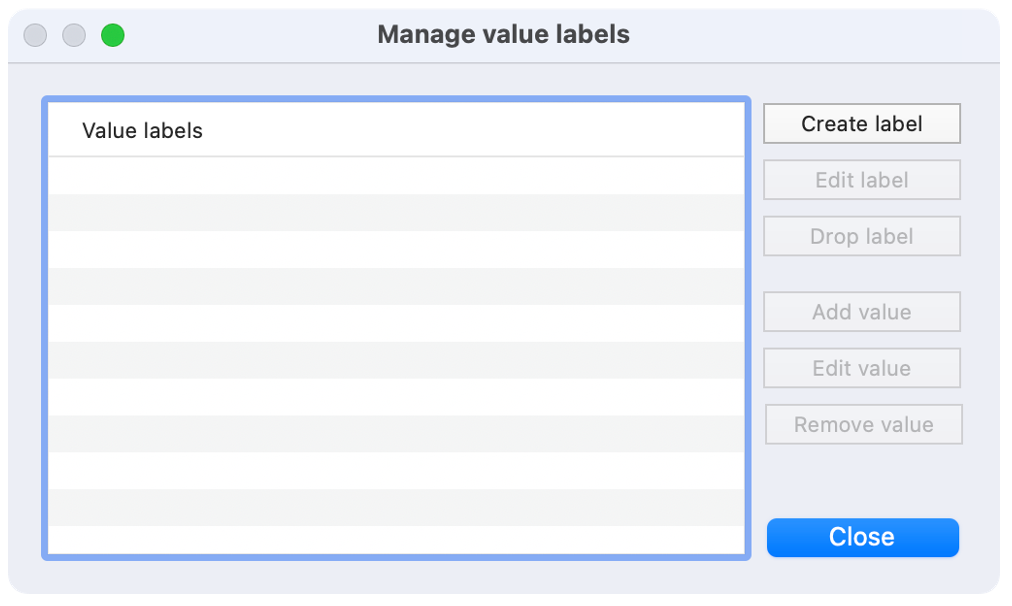
\includegraphics[width=0.75\linewidth]{img/mod01/stata/value-labels-01}

In the \textbf{Manage value labels} dialog box, click the \textbf{Create label} button.

\begin{enumerate}
\def\labelenumi{\arabic{enumi}.}
\setcounter{enumi}{1}
\item
  In the next dialog box, enter a name for the value label such as \texttt{sex\_label} in the \textbf{Label name:} box. You can use the same name of the variable for the label, or choose a different name. Note: as for variables, the value label name is case-sensitive.
\item
  Next, we specify what each category (i.e.~1 and 2) represents. By checking the metadata document, we see that \texttt{1} represents ``Male'' and \texttt{2} represents ``Female''. Type the number \texttt{1} in the \textbf{Value:} box and the word \texttt{Male} in the \textbf{Label:} box; then click the \textbf{Add} button. Then type the number \texttt{2} in the \textbf{Value:} box and the word \texttt{Female} in the \textbf{Label:} box; click the \textbf{Add} button again. The defined value labels for males and females should appear in the box on the left-hand side. When you are done, click the \textbf{OK} button.
\end{enumerate}

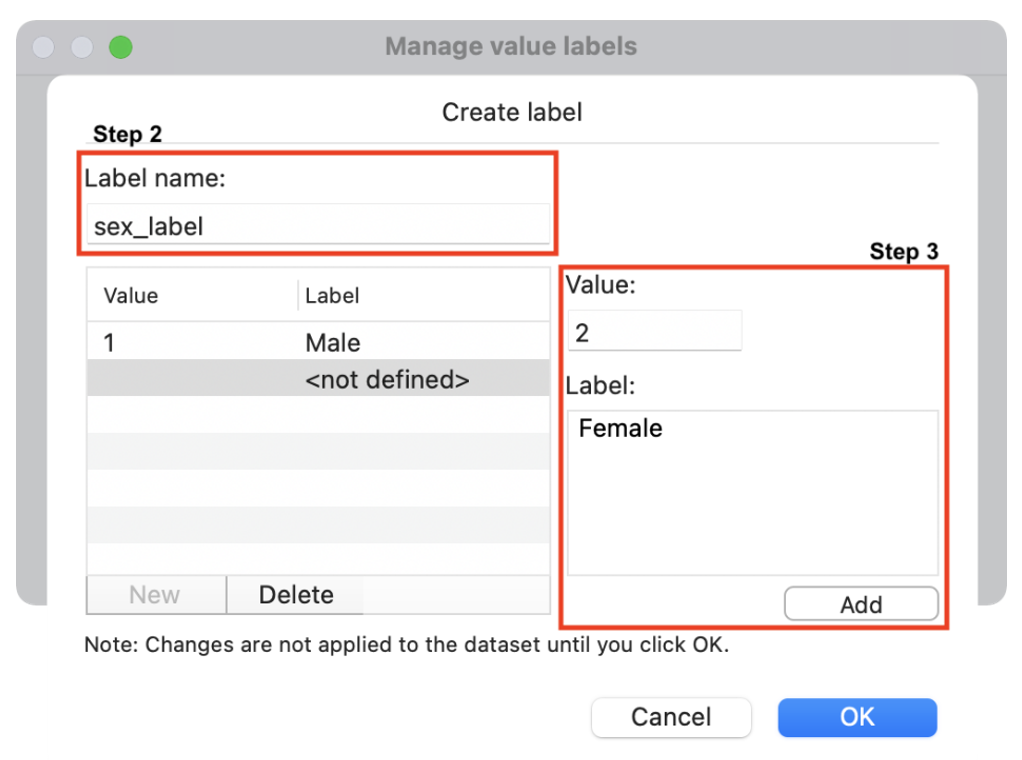
\includegraphics[width=0.75\linewidth]{img/mod01/stata/value-labels-02}

You will be returned to the \textbf{Manage value labels} dialog box, which will now have a record for \texttt{sex\_label}. By clicking the arrow next to the label name, you will see the codes that you have defined:

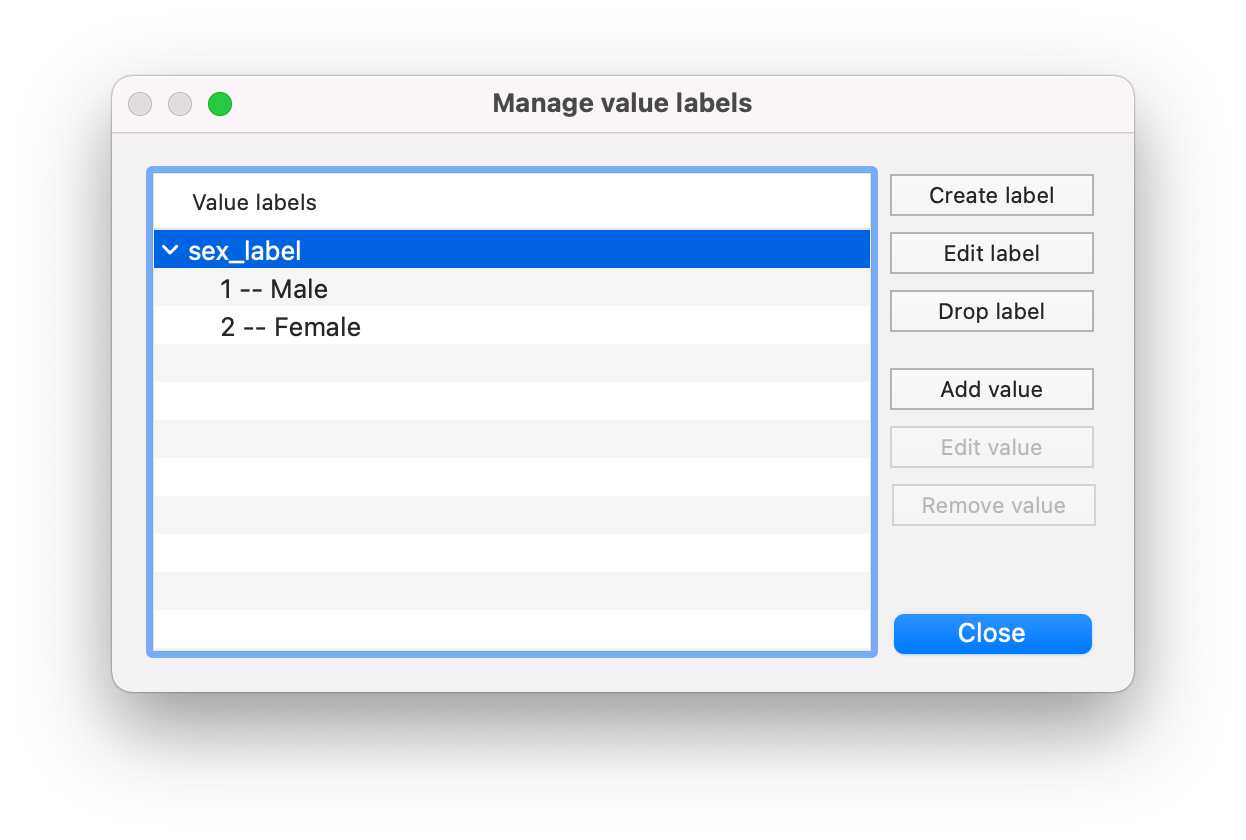
\includegraphics[width=0.75\linewidth]{img/mod01/stata/value-labels-03}

At this point, you can close the \textbf{Manage value labels} dialog box by clicking \textbf{Close}.

\textbf{Part 2:} Applying the value labels to a variable

Now that the labels are defined, we need to attach them to the relevant variables. Within the Variables Manager, click the variable to be labelled (here, \texttt{sex}). The previously defined label can be assigned to this variable by clicking the \textbf{Value label} drop-down menu, and choosing the appropriate label (here, \texttt{sex\_label}), and clicking \textbf{Apply}:

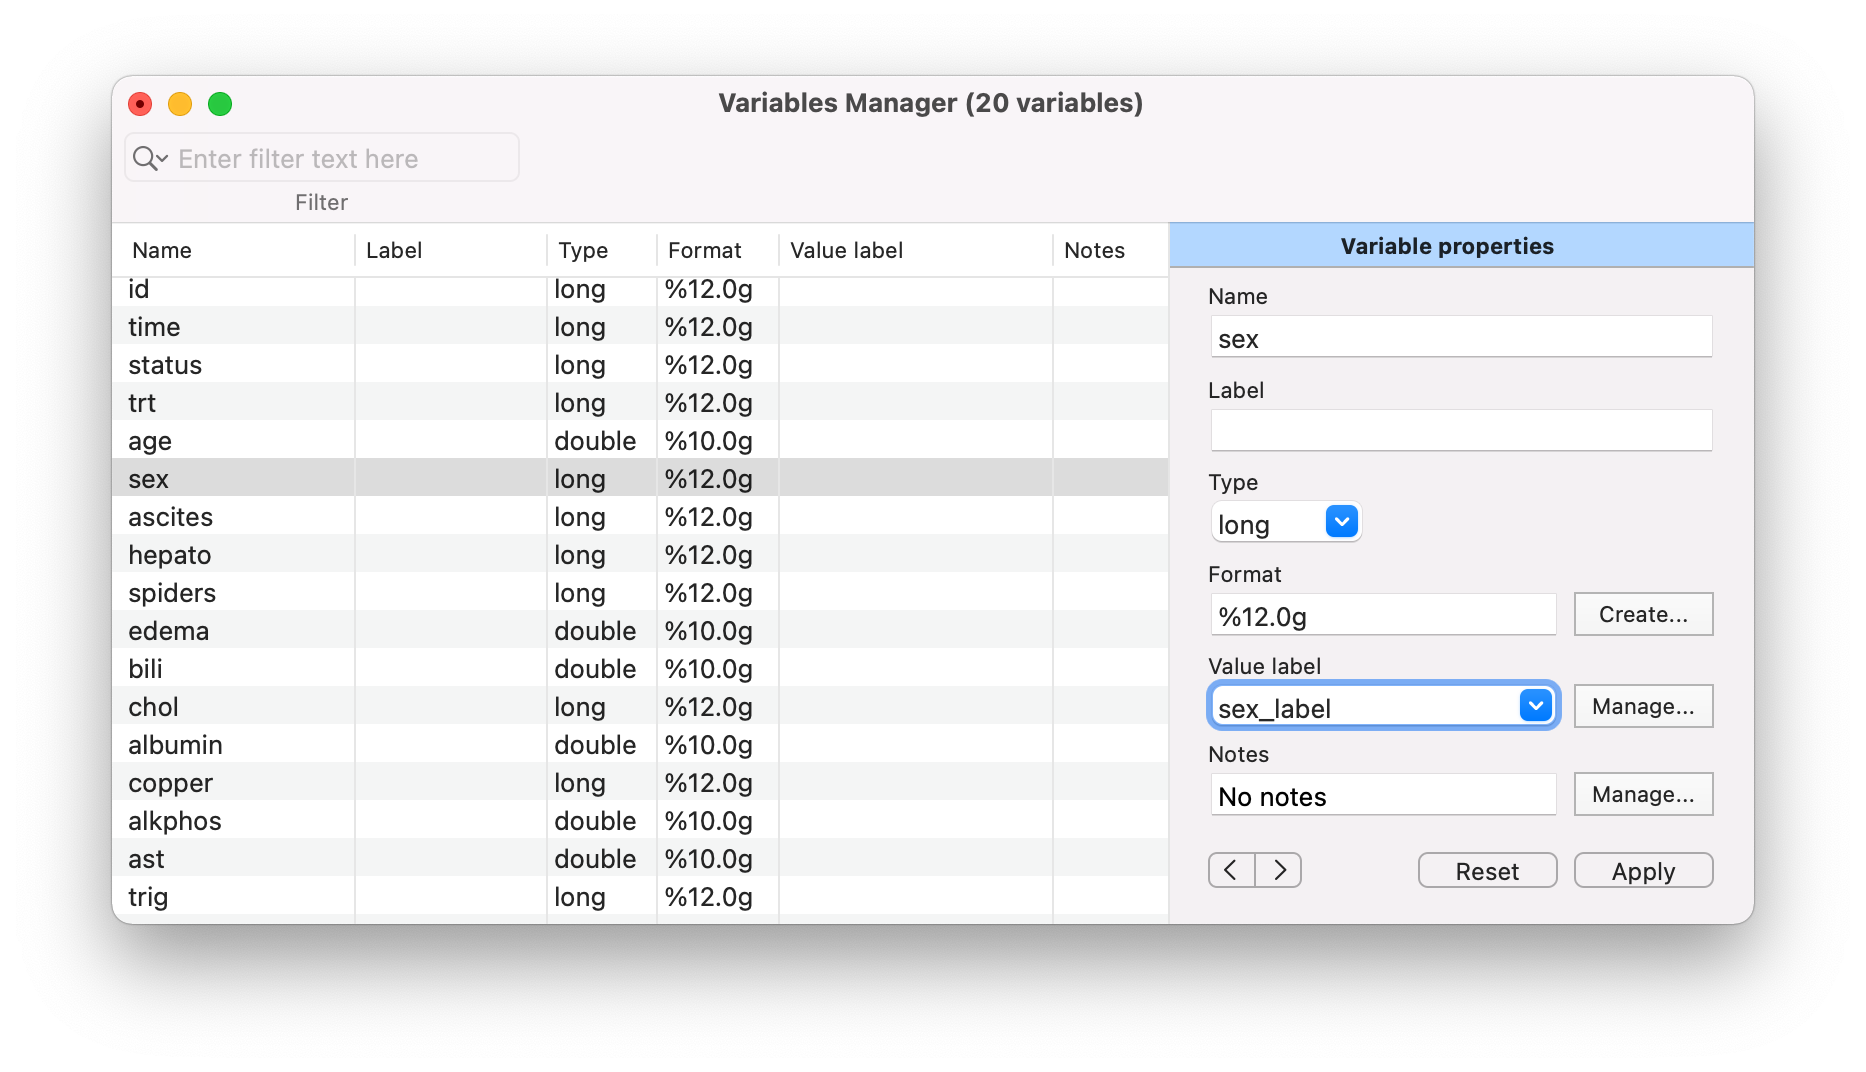
\includegraphics[width=0.75\linewidth]{img/mod01/stata/value-labels-04-1}

Alternatively, go to \textbf{Data \textgreater{} Data utilities \textgreater{} Label utilities \textgreater{} Assign value label to variables}. Select \texttt{sex} from the \textbf{Variables:} dropdown box, and select \texttt{sex\_label} from the \textbf{Value label:} dropdown box. Click \textbf{OK}.

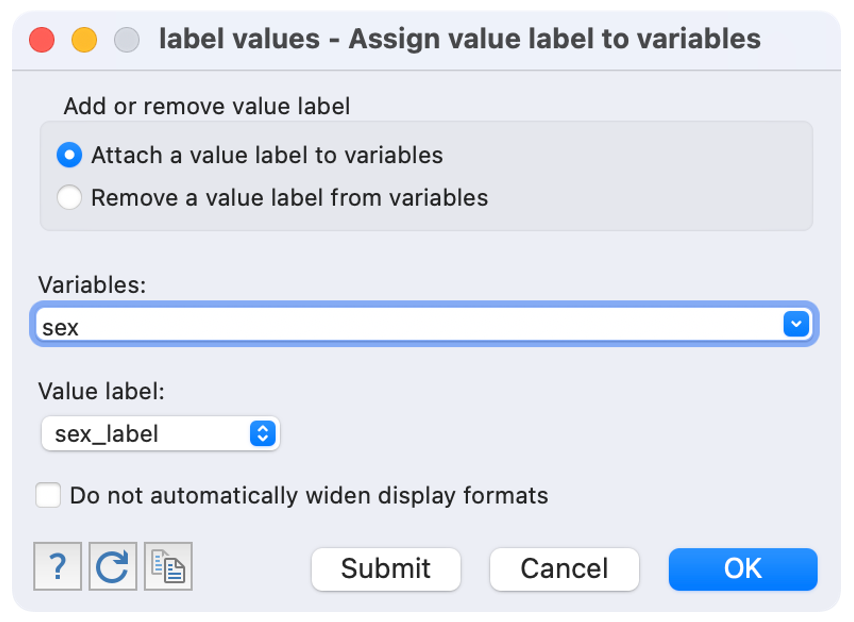
\includegraphics[width=0.75\linewidth]{img/mod01/stata/value-labels-04}

There are a number of ways that we can confirm that the labelling has been done correctly. One of the easiest ways is to use the \texttt{codebook} command to investigate the coding of sex: \textbf{Data \textgreater{} Describe data \textgreater{} Describe data contents (codebook)}.

\begin{Shaded}
\begin{Highlighting}[]
\NormalTok{. codebook sex}

\NormalTok{{-}{-}{-}{-}{-}{-}{-}{-}{-}{-}{-}{-}{-}{-}{-}{-}{-}{-}{-}{-}{-}{-}{-}{-}{-}{-}{-}{-}{-}{-}{-}{-}{-}{-}{-}{-}{-}{-}{-}{-}{-}{-}{-}{-}{-}{-}{-}{-}{-}{-}{-}{-}{-}{-}{-}{-}{-}{-}{-}{-}{-}{-}{-}{-}{-}{-}{-}{-}{-}{-}{-}{-}{-}{-}{-}{-}{-}{-}{-}{-}{-}{-}{-}{-}{-}{-}{-}{-}}
\NormalTok{sex                                                                          (unlabeled)}
\NormalTok{{-}{-}{-}{-}{-}{-}{-}{-}{-}{-}{-}{-}{-}{-}{-}{-}{-}{-}{-}{-}{-}{-}{-}{-}{-}{-}{-}{-}{-}{-}{-}{-}{-}{-}{-}{-}{-}{-}{-}{-}{-}{-}{-}{-}{-}{-}{-}{-}{-}{-}{-}{-}{-}{-}{-}{-}{-}{-}{-}{-}{-}{-}{-}{-}{-}{-}{-}{-}{-}{-}{-}{-}{-}{-}{-}{-}{-}{-}{-}{-}{-}{-}{-}{-}{-}{-}{-}{-}}

\NormalTok{                  type:  numeric (long)}
\NormalTok{                 label:  sex\_label}

\NormalTok{                 range:  [1,2]                        units:  1}
\NormalTok{         unique values:  2                        missing .:  0/418}

\NormalTok{            tabulation:  Freq.   Numeric  Label}
\NormalTok{                            44         1  Male}
\NormalTok{                           374         2  Female}
\end{Highlighting}
\end{Shaded}

Here we can see that the codes for male and female have been applied correctly. We can also examine the Data Browser and confirm that sex has been labelled.

Note: If you want to see the original coded values of the labelled groups in the Data Browser window, you can hide the value labels by choosing \textbf{Tools \textgreater{} Value labels \textgreater{} Hide all value labels} for Windows, or \textbf{View \textgreater{} Value labels \textgreater{} Hide all value labels} for Mac from the menu bar in the Data Browser window.

\textbf{TASK:} create and apply value labels for Vital Status.

Now that our categorical variables are labelled, we can produce the one-way frequency tables. As before, choose \textbf{Statistics \textgreater{} Summaries, tables, and tests \textgreater{} Frequency tables \textgreater{} One-way table}. Our newly labelled table for sex appears as below.

\begin{Shaded}
\begin{Highlighting}[]
\NormalTok{        sex |      Freq.     Percent        Cum.}
\NormalTok{{-}{-}{-}{-}{-}{-}{-}{-}{-}{-}{-}{-}+{-}{-}{-}{-}{-}{-}{-}{-}{-}{-}{-}{-}{-}{-}{-}{-}{-}{-}{-}{-}{-}{-}{-}{-}{-}{-}{-}{-}{-}{-}{-}{-}{-}{-}{-}}
\NormalTok{       Male |         44       10.53       10.53}
\NormalTok{     Female |        374       89.47      100.00}
\NormalTok{{-}{-}{-}{-}{-}{-}{-}{-}{-}{-}{-}{-}+{-}{-}{-}{-}{-}{-}{-}{-}{-}{-}{-}{-}{-}{-}{-}{-}{-}{-}{-}{-}{-}{-}{-}{-}{-}{-}{-}{-}{-}{-}{-}{-}{-}{-}{-}}
\NormalTok{      Total |        418      100.00}
\end{Highlighting}
\end{Shaded}

\textbf{TASK:} produce one-way frequency tables for the other categorical variables in Table 1 (stage and vital status).

\hypertarget{producing-a-two-way-frequency-table}{%
\subsection{Producing a two-way frequency table}\label{producing-a-two-way-frequency-table}}

To produce tables summarising two categorical variables, go to \textbf{Statistics - Summaries, tables, and tests - Frequency tables - Two-way table with measures of association}.

To produce a two-way table showing stage of disease by sex using the pbc.dta data, do the following. In the \textbf{tabulate2 -- two way table with measures of association dialog box}, select the variable \texttt{sex} as the \textbf{Row variable:}, and \texttt{stage} as the \textbf{Column variable:} as shown below.

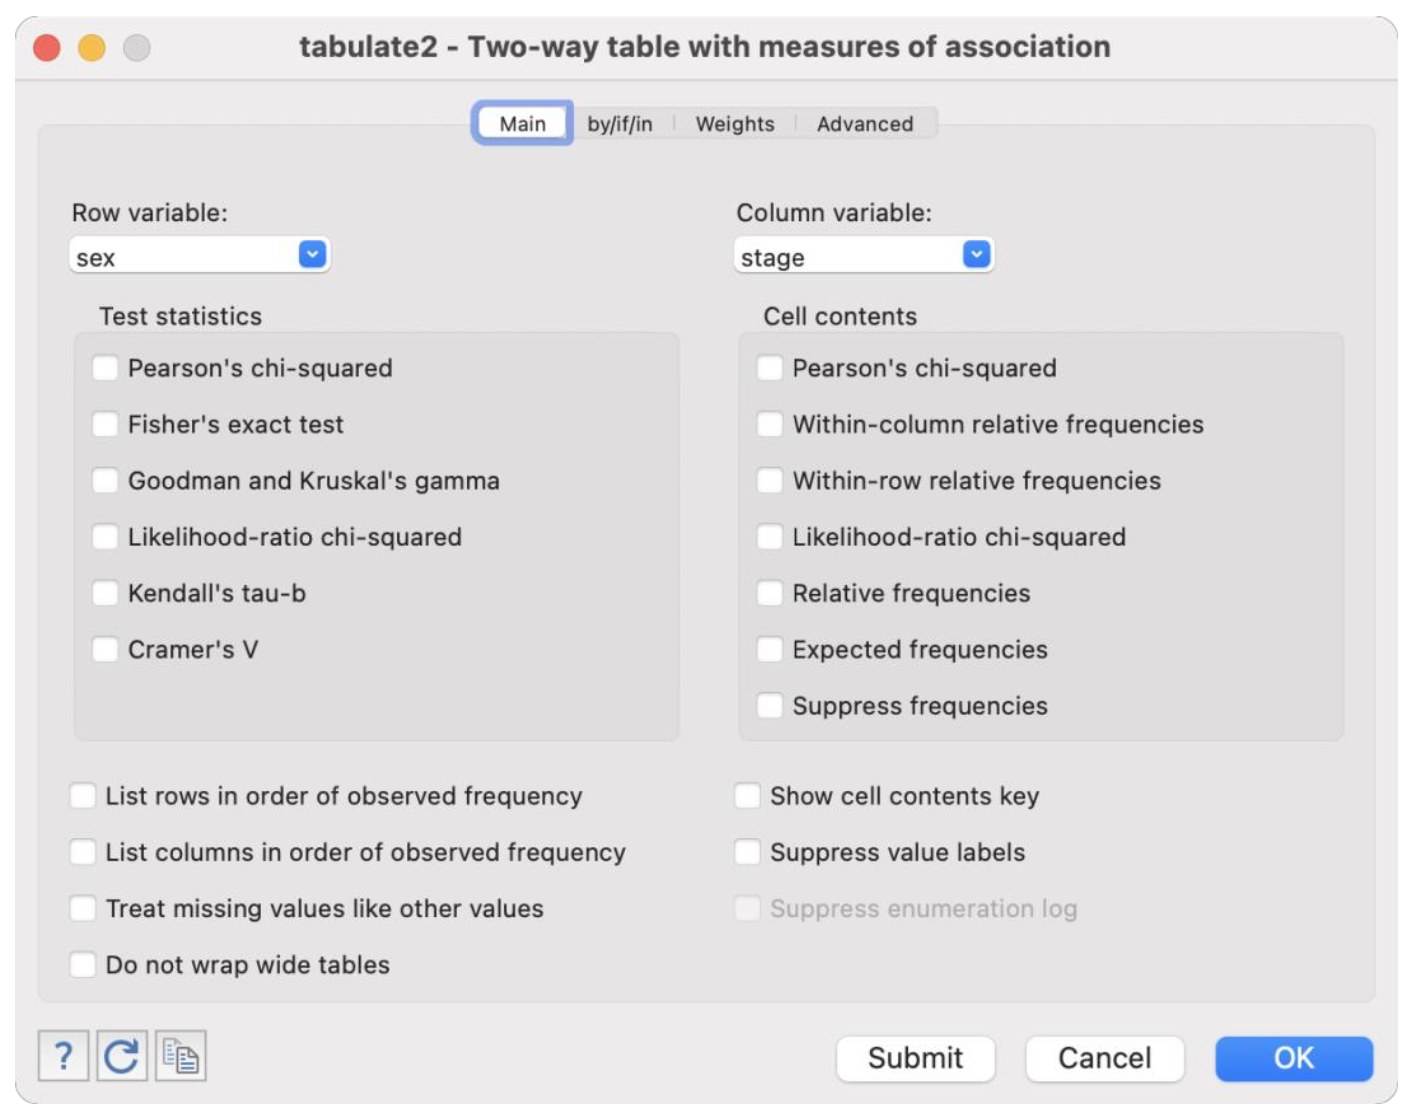
\includegraphics[width=0.75\linewidth]{img/mod01/stata/mod01-twoway}

Click \textbf{OK} to obtain the output below.

\begin{Shaded}
\begin{Highlighting}[]
\NormalTok{. tabulate sex stage}

\NormalTok{           |                    stage}
\NormalTok{       sex |   Stage 1    Stage 2    Stage 3    Stage 4 |     Total}
\NormalTok{{-}{-}{-}{-}{-}{-}{-}{-}{-}{-}{-}+{-}{-}{-}{-}{-}{-}{-}{-}{-}{-}{-}{-}{-}{-}{-}{-}{-}{-}{-}{-}{-}{-}{-}{-}{-}{-}{-}{-}{-}{-}{-}{-}{-}{-}{-}{-}{-}{-}{-}{-}{-}{-}{-}{-}+{-}{-}{-}{-}{-}{-}{-}{-}{-}{-}}
\NormalTok{      Male |         3          8         16         17 |        44 }
\NormalTok{    Female |        18         84        139        127 |       368 }
\NormalTok{{-}{-}{-}{-}{-}{-}{-}{-}{-}{-}{-}+{-}{-}{-}{-}{-}{-}{-}{-}{-}{-}{-}{-}{-}{-}{-}{-}{-}{-}{-}{-}{-}{-}{-}{-}{-}{-}{-}{-}{-}{-}{-}{-}{-}{-}{-}{-}{-}{-}{-}{-}{-}{-}{-}{-}+{-}{-}{-}{-}{-}{-}{-}{-}{-}{-}}
\NormalTok{     Total |        21         92        155        144 |       412 }
\end{Highlighting}
\end{Shaded}

You may notice in the above that the number of observations is now 412. This is because there are missing observations for either sex or stage: which is it, and how would you determine this?

From the cross-tabulation, you can see the individual frequencies of participants in each of the categories in each cell. For example, there are 3 male participants who have Stage 1 disease. You can also read the totals for each row and column. For example, there are 44 males, and 144 participants have Stage 4 disease.

You can also add percentages into your table. For example, in the \textbf{tabulate2 -- two way table with measures of association} dialog box tick the box \textbf{Within-column relative frequencies} for separate percentages of sex within each stage.

\begin{Shaded}
\begin{Highlighting}[]
\NormalTok{. tabulate sex stage, column}

\NormalTok{+{-}{-}{-}{-}{-}{-}{-}{-}{-}{-}{-}{-}{-}{-}{-}{-}{-}{-}{-}+}
\NormalTok{| Key               |}
\NormalTok{|{-}{-}{-}{-}{-}{-}{-}{-}{-}{-}{-}{-}{-}{-}{-}{-}{-}{-}{-}|}
\NormalTok{|     frequency     |}
\NormalTok{| column percentage |}
\NormalTok{+{-}{-}{-}{-}{-}{-}{-}{-}{-}{-}{-}{-}{-}{-}{-}{-}{-}{-}{-}+}

\NormalTok{           |                    stage}
\NormalTok{       sex |   Stage 1    Stage 2    Stage 3    Stage 4 |     Total}
\NormalTok{{-}{-}{-}{-}{-}{-}{-}{-}{-}{-}{-}+{-}{-}{-}{-}{-}{-}{-}{-}{-}{-}{-}{-}{-}{-}{-}{-}{-}{-}{-}{-}{-}{-}{-}{-}{-}{-}{-}{-}{-}{-}{-}{-}{-}{-}{-}{-}{-}{-}{-}{-}{-}{-}{-}{-}+{-}{-}{-}{-}{-}{-}{-}{-}{-}{-}}
\NormalTok{      Male |         3          8         16         17 |        44 }
\NormalTok{           |     14.29       8.70      10.32      11.81 |     10.68 }
\NormalTok{{-}{-}{-}{-}{-}{-}{-}{-}{-}{-}{-}+{-}{-}{-}{-}{-}{-}{-}{-}{-}{-}{-}{-}{-}{-}{-}{-}{-}{-}{-}{-}{-}{-}{-}{-}{-}{-}{-}{-}{-}{-}{-}{-}{-}{-}{-}{-}{-}{-}{-}{-}{-}{-}{-}{-}+{-}{-}{-}{-}{-}{-}{-}{-}{-}{-}}
\NormalTok{    Female |        18         84        139        127 |       368 }
\NormalTok{           |     85.71      91.30      89.68      88.19 |     89.32 }
\NormalTok{{-}{-}{-}{-}{-}{-}{-}{-}{-}{-}{-}+{-}{-}{-}{-}{-}{-}{-}{-}{-}{-}{-}{-}{-}{-}{-}{-}{-}{-}{-}{-}{-}{-}{-}{-}{-}{-}{-}{-}{-}{-}{-}{-}{-}{-}{-}{-}{-}{-}{-}{-}{-}{-}{-}{-}+{-}{-}{-}{-}{-}{-}{-}{-}{-}{-}}
\NormalTok{     Total |        21         92        155        144 |       412 }
\NormalTok{           |    100.00     100.00     100.00     100.00 |    100.00 }
\end{Highlighting}
\end{Shaded}

We can see that the 3 male participants with Stage 1 disease made up 14\% of those with Stage 1 disease.

\hypertarget{saving-data-from-stata}{%
\subsection{Saving data from Stata}\label{saving-data-from-stata}}

Now that you have made some changes to the pbc data, it is good practice to save the dataset. Stata uses its own file format to save data. Data saved from Stata will end with the .dta suffix, and will contain useful information such as variable labels and value labels, as well as any new variables created. However, data saved by Stata will only be able to be opened by Stata - you will not easily be able to share your data with colleagues who do not have Stata. To save a Stata dataset, choose \textbf{File \textgreater{} Save}.

If you want to share data with colleagues who do not have Stata, you can use \textbf{File \textgreater{} Export} to save your data in another file format (recognising that variable and value labels will not be exported.)

\hypertarget{copying-output-from-stata}{%
\subsection{Copying output from Stata}\label{copying-output-from-stata}}

It is important to note that \emph{saving data in Stata will not save your output}. Stata data and output are completely separate to one another. The easiest way to retain the output of your analyses is to copy the output into a word processor package (e.g.~Microsoft Word) before closing Stata. Once Stata is closed, all the output (that is, all your hard work!) is lost.

To copy output from Stata, you can select the output and choose \textbf{Edit \textgreater{} Copy}. This will copy the output as plain text for pasting into a Word document. If you select a single table for copying, you can also \textbf{Copy table} or \textbf{Copy table as HTML}. Whichever way you copy output into Word, you will need to make sure you reformat the table and relabel your header row and column properly for your assignments as described in Module 1. Alternatively, you can copy with the Copy table option for pasting into an Excel worksheet and reformat your table in Excel before pasting into Word.

Copying output from Stata can get a little complicated to explain. We have included a video on Moodle to summarise the different ways output can be copied.

\textbf{TASK:} complete Table 1 using the output generated in this exercise. You should decide on whether to present continuous variables by their means or medians, and present the most appropriate measure of spread. Include footnotes to indicate if any variables contain missing observations.

\hypertarget{part-3-creating-other-types-of-graphs}{%
\section*{Part 3: Creating other types of graphs}\label{part-3-creating-other-types-of-graphs}}
\addcontentsline{toc}{section}{Part 3: Creating other types of graphs}

\hypertarget{bar-graphs-1}{%
\subsection{Bar graphs}\label{bar-graphs-1}}

Here we will create the bar chart shown in Figure \ref{fig:fig-1-1} using the \texttt{pbc.dta} dataset. The x-axis of this graph will be the stage of disease, and the y-axis will show the number of participants in each category.

To create a Bar chart, go to the Stata menu Graphics \textgreater{} Bar chart and the bar-chart dialog box will appear.

\hypertarget{simple-bar-graph}{%
\subsubsection{Simple bar graph}\label{simple-bar-graph}}

For most of our bar graphs, we will be plotting frequencies, so we choose \textbf{Graph of frequencies within categories}

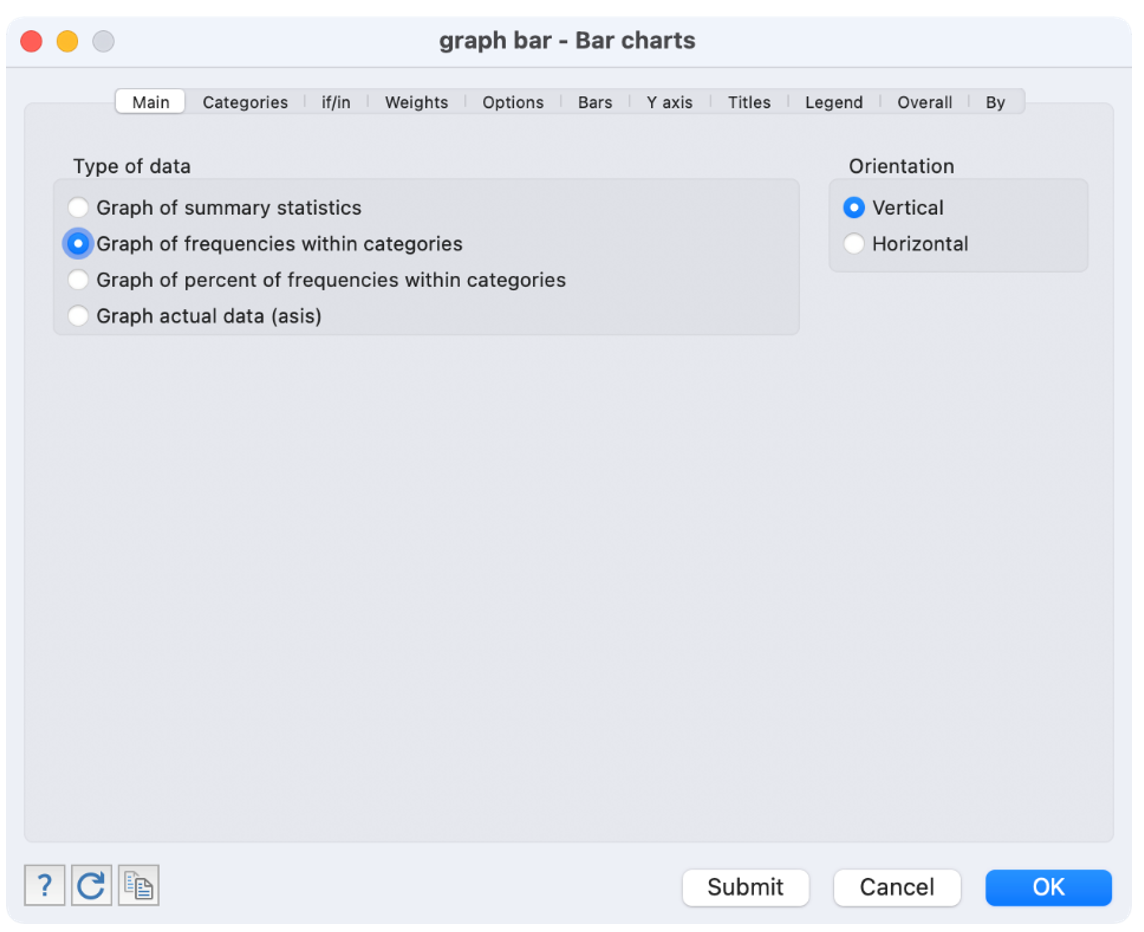
\includegraphics[width=0.75\linewidth]{img/mod01/stata/bar-01}

For a simple bar graph, go to the \textbf{Categories} tab, tick the \textbf{Group 1} box and choose \texttt{stage} as your first grouping variable:

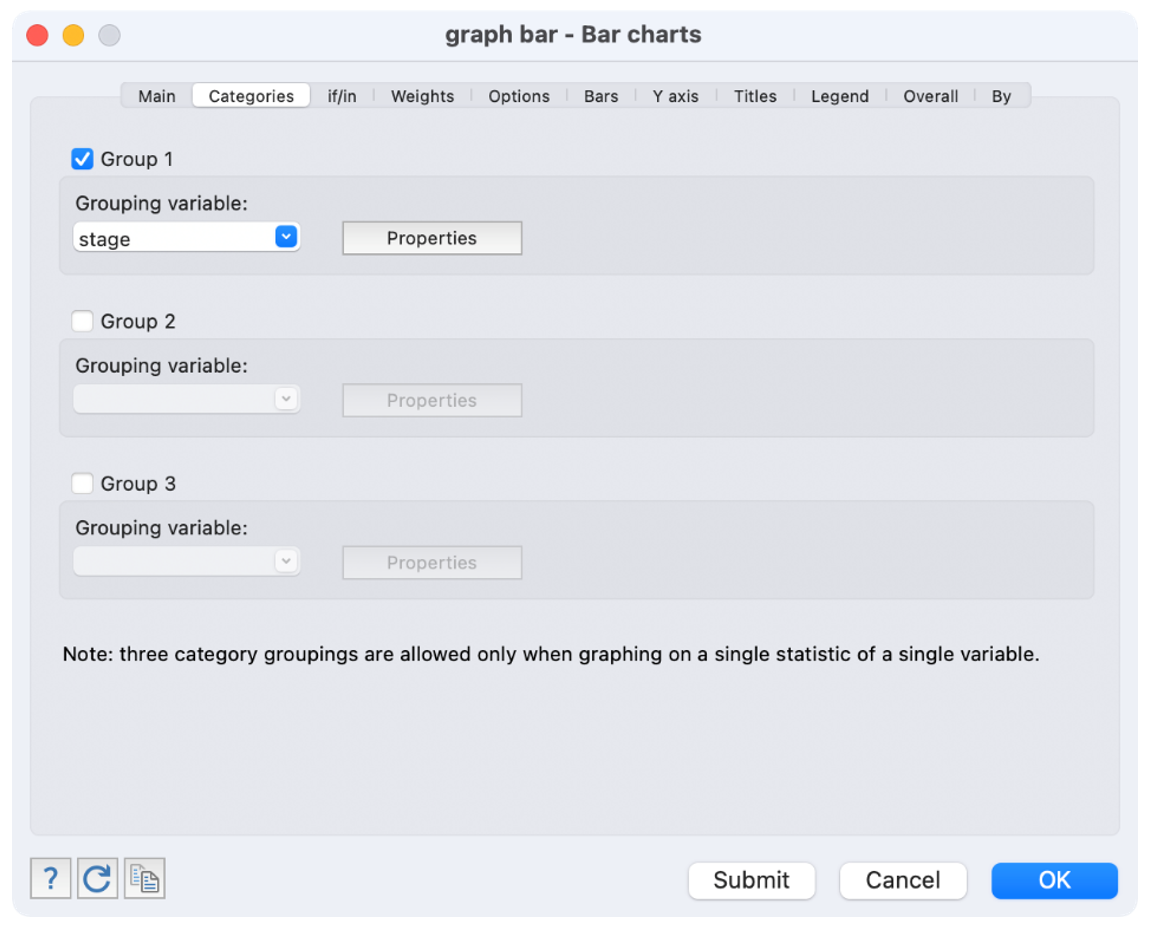
\includegraphics[width=0.75\linewidth]{img/mod01/stata/bar-02}

Click the \textbf{Y axis} tab to include a more meaningful label for the y axis:

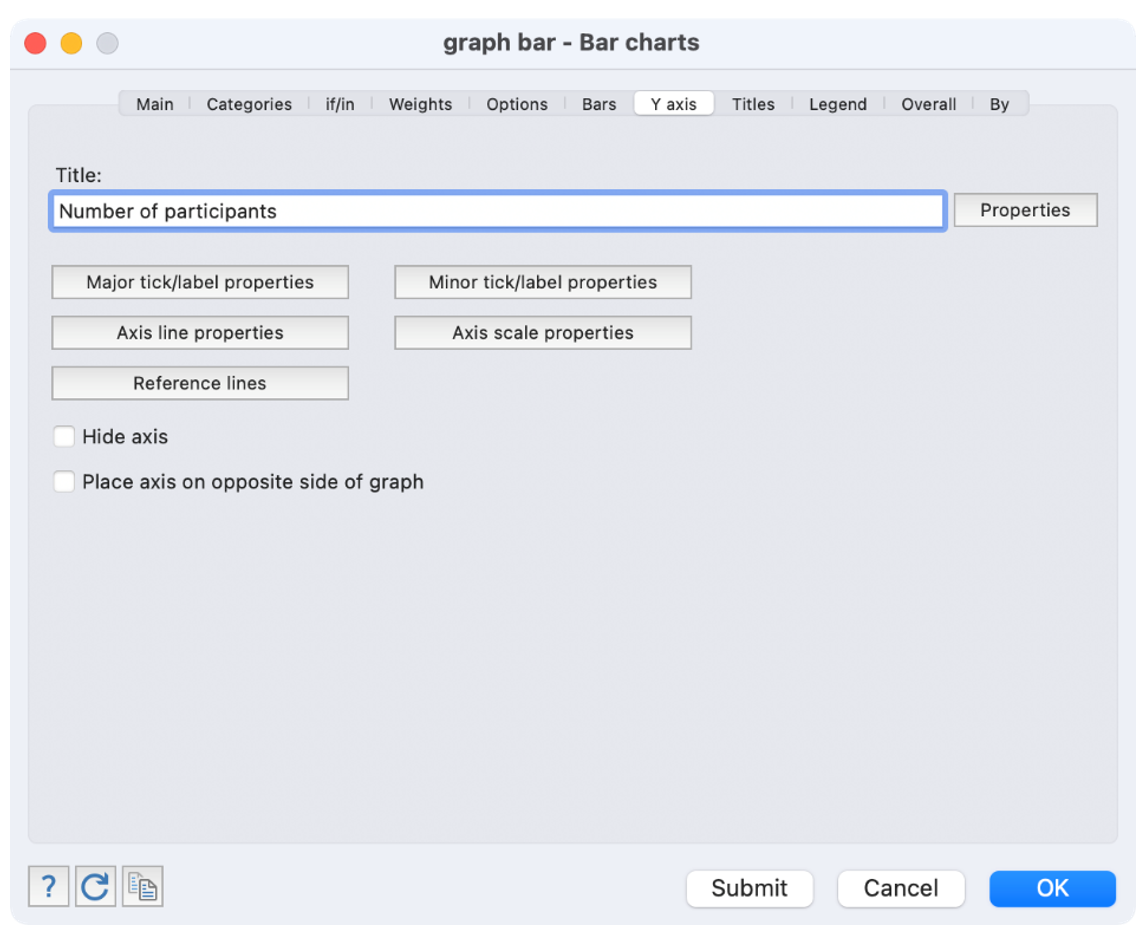
\includegraphics[width=0.75\linewidth]{img/mod01/stata/bar-03}

Click \textbf{Submit} or \textbf{OK}, and the following graph will appear:

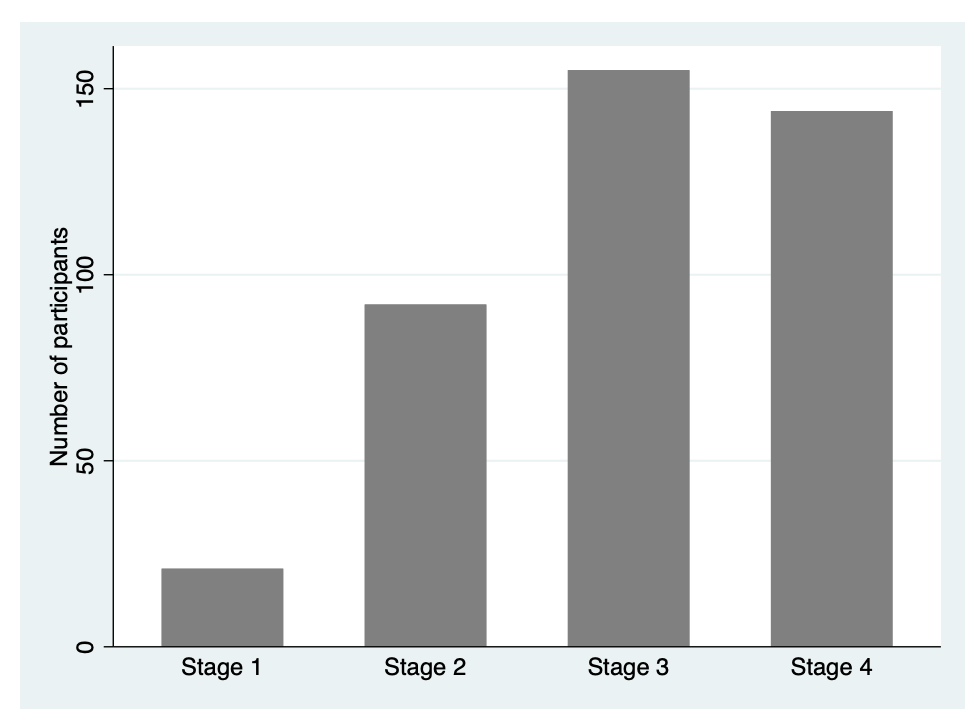
\includegraphics[width=0.75\linewidth]{img/mod01/stata/bar-04}

Note: Value labels have been assigned to stage to create more meaningful output, and bar colours have been changed to allow for grey-scale printing.

\hypertarget{submit-vs-ok-button}{%
\subsection{Submit vs OK button}\label{submit-vs-ok-button}}

You may note that most dialog boxes in Stata have two choices: the \textbf{Submit} button, and the \textbf{OK} button. Both buttons will submit the command to be run, and both will produce a graph. The \textbf{Submit} button will submit the command but leave the dialog box open, while the \textbf{OK} button will submit the command and close the dialog box. Given the building a graph often involves many incremental changes, the \textbf{Submit} button is a useful option.

\hypertarget{clustered-bar-graph}{%
\subsection{Clustered bar graph}\label{clustered-bar-graph}}

To create a clustered bar chart as shown in Figure \ref{fig:fig-1-2}, go to: \textbf{Graphics \textgreater{} Bar chart} again. With the previous settings in place (i.e.~stage as grouping variable and with appropriate axes labels), now choose \texttt{sex} as the \textbf{Group 1} variable, and tick \textbf{Group 2} and choose \texttt{stage} as the second grouping variable.

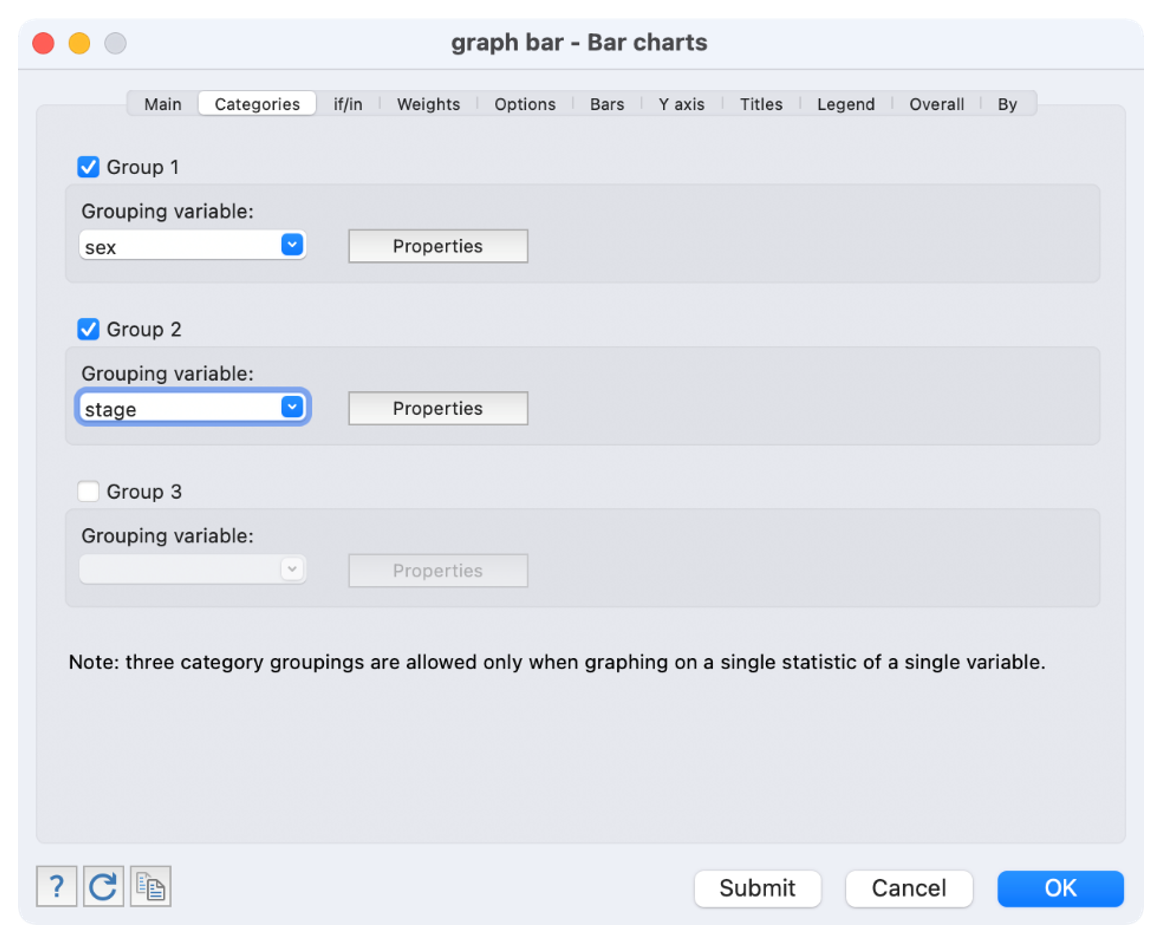
\includegraphics[width=0.75\linewidth]{img/mod01/stata/bar-05}

In the \textbf{Options} tab, tick \textbf{Treat first category grouping as y variables}. When you are done, click \textbf{OK} or \textbf{Submit}.

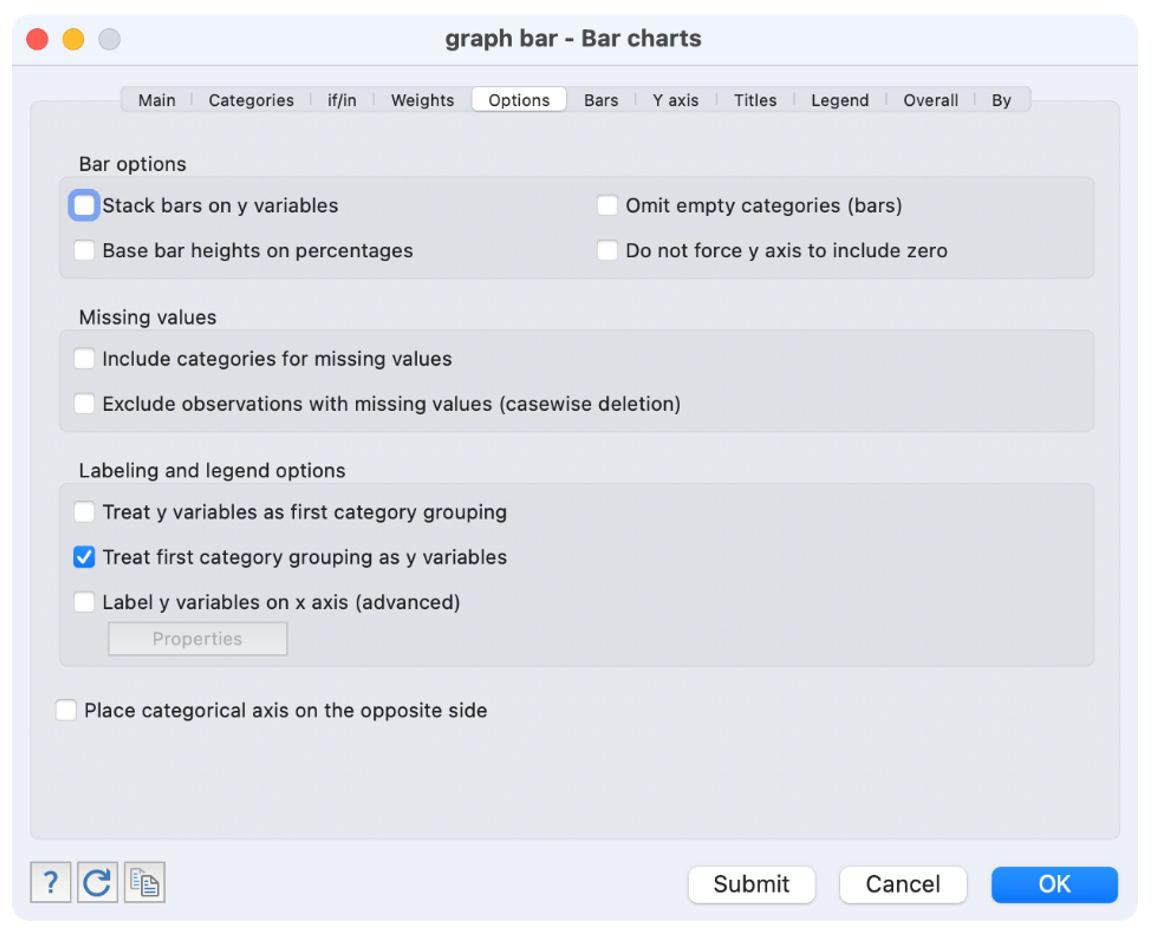
\includegraphics[width=0.75\linewidth]{img/mod01/stata/bar-06}

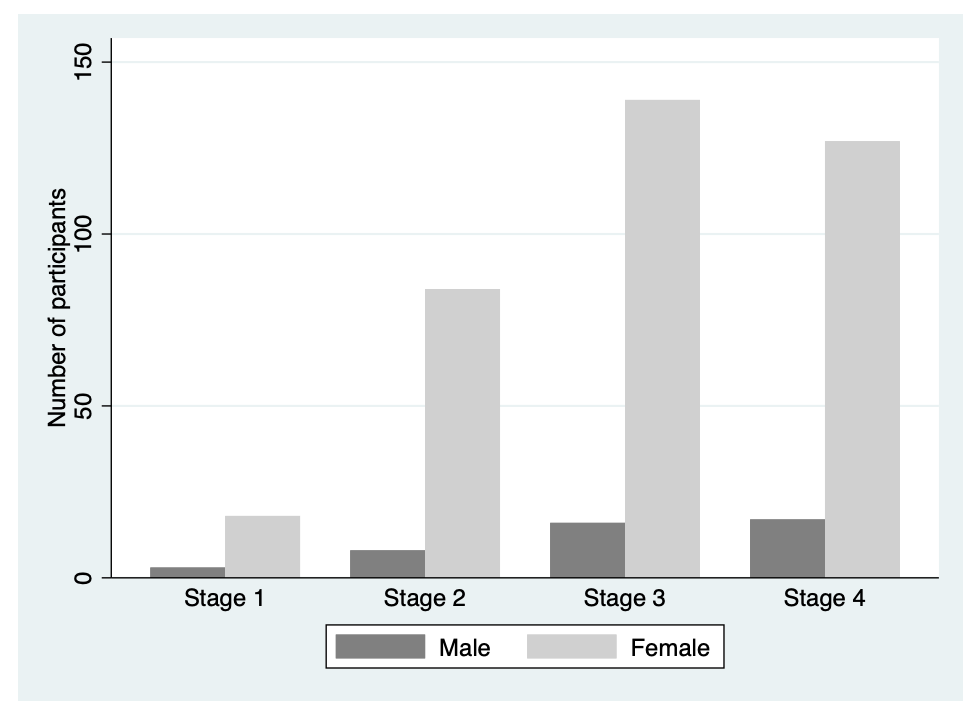
\includegraphics[width=0.75\linewidth]{img/mod01/stata/bar-07}

In a clustered bar chart, the \textbf{Group 2} variable is the main variable grouping (here, \texttt{stage}), and each of the \textbf{Group 2} categories is split by the \textbf{Group 1} variable (here, \texttt{sex}).

\hypertarget{stacked-bar-graph}{%
\subsection{Stacked bar graph}\label{stacked-bar-graph}}

To create a stacked bar chart shown in Figure \ref{fig:fig-1-3}, bring up the \textbf{Bar chart} dialog box, go to the \textbf{Options} tab and tick \textbf{Stack bars on y variables}.

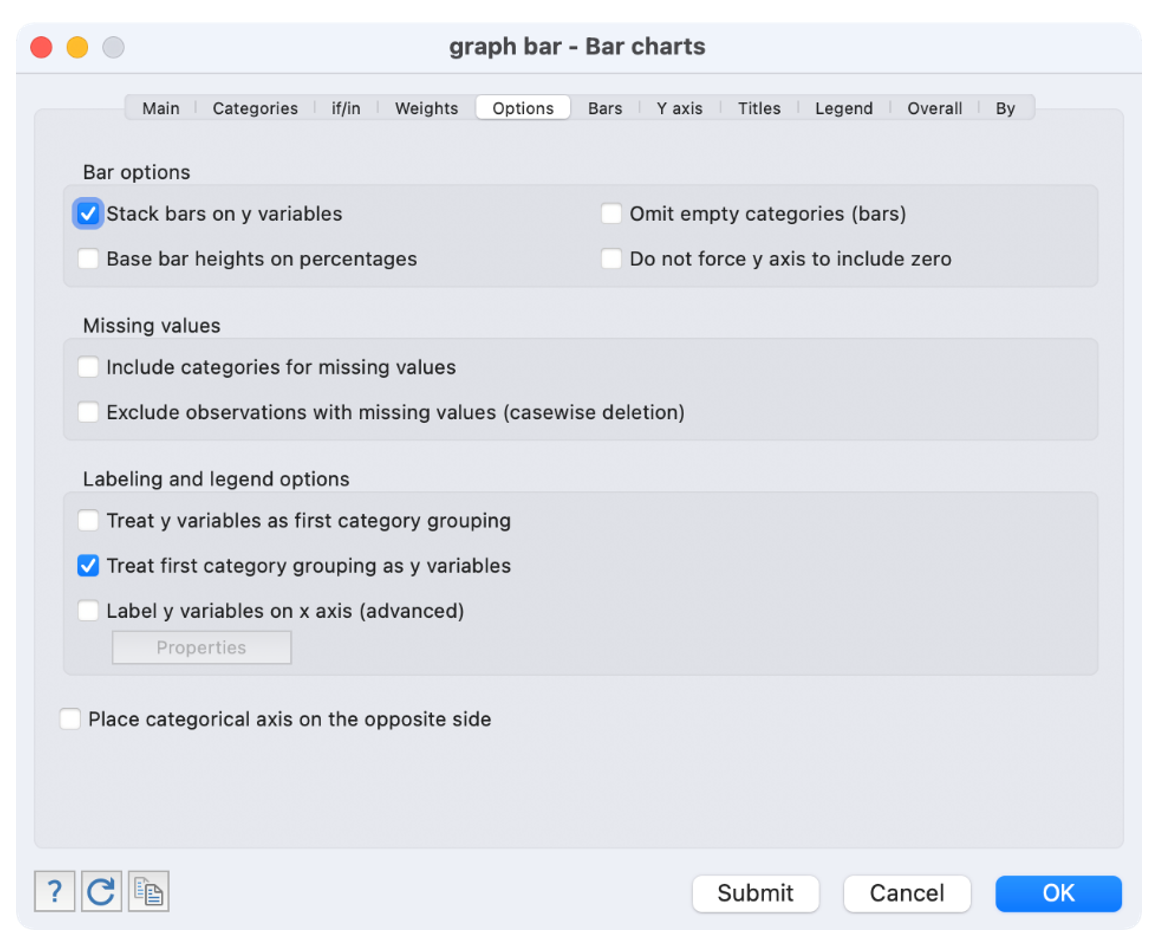
\includegraphics[width=0.75\linewidth]{img/mod01/stata/bar-08}

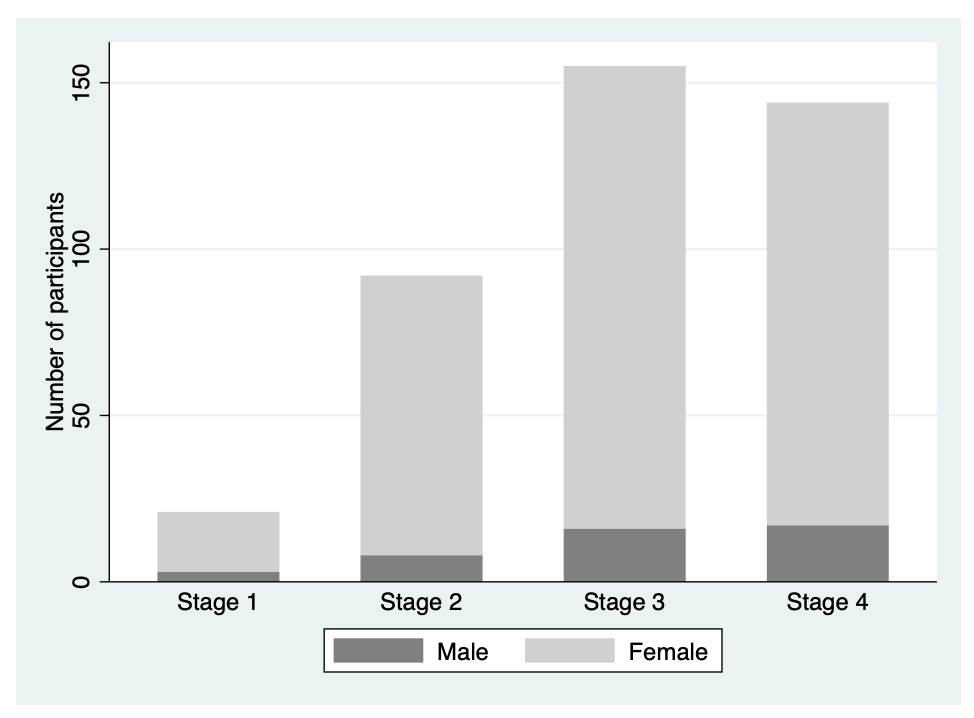
\includegraphics[width=0.75\linewidth]{img/mod01/stata/bar-10}

\hypertarget{stacked-bar-graph-of-relative-frequencies}{%
\subsection{Stacked bar graph of relative frequencies}\label{stacked-bar-graph-of-relative-frequencies}}

If one wants to compare the sex distribution across the stage categories, it would be convenient if all the bars have the same height (100\%). To generate such a bar chart in Stata, tick \textbf{Base bar heights on percentages} in the \textbf{Options} tab of the \textbf{Bar charts} dialog box. Change the y-axis title in the \textbf{Y axis} tab to \texttt{Percentage\ of\ students\ in\ each\ age\ group}.

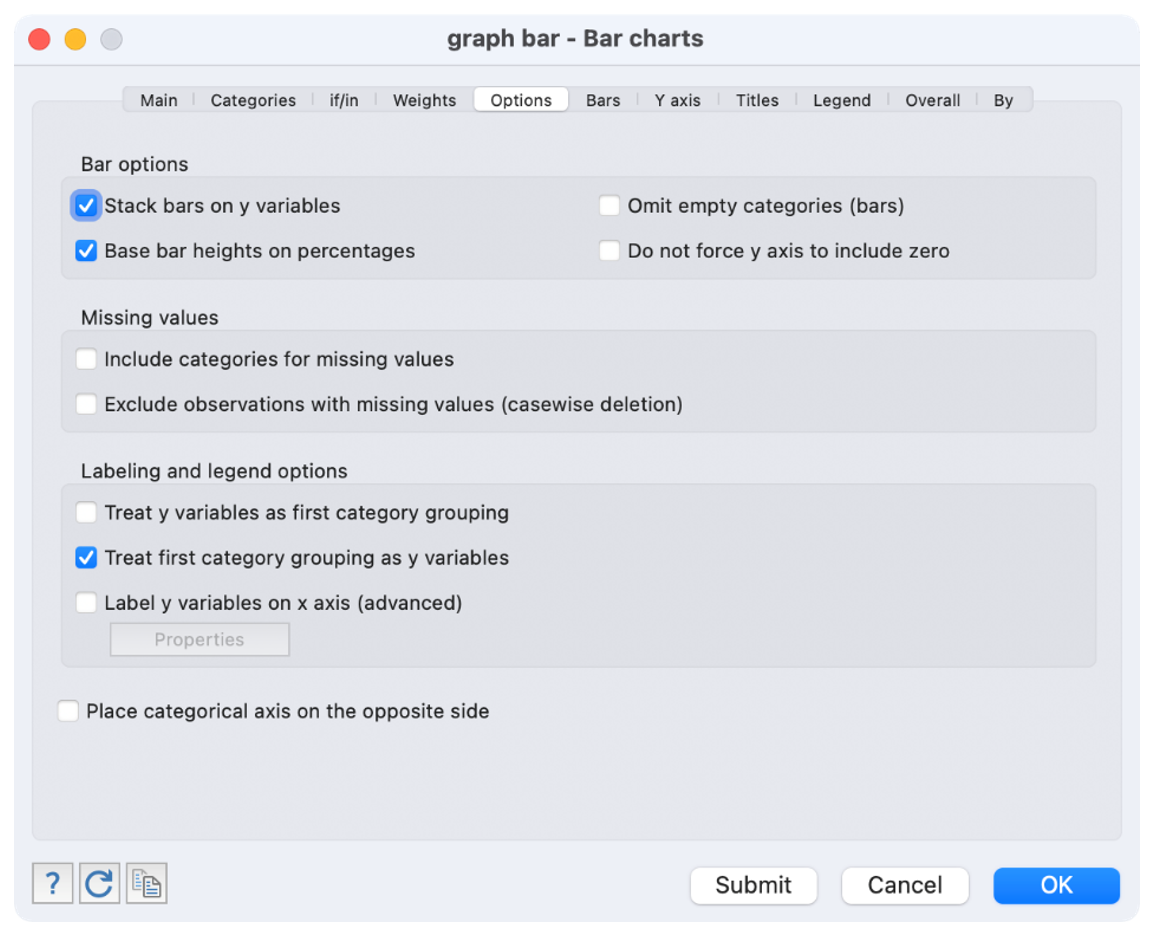
\includegraphics[width=0.75\linewidth]{img/mod01/stata/bar-11}

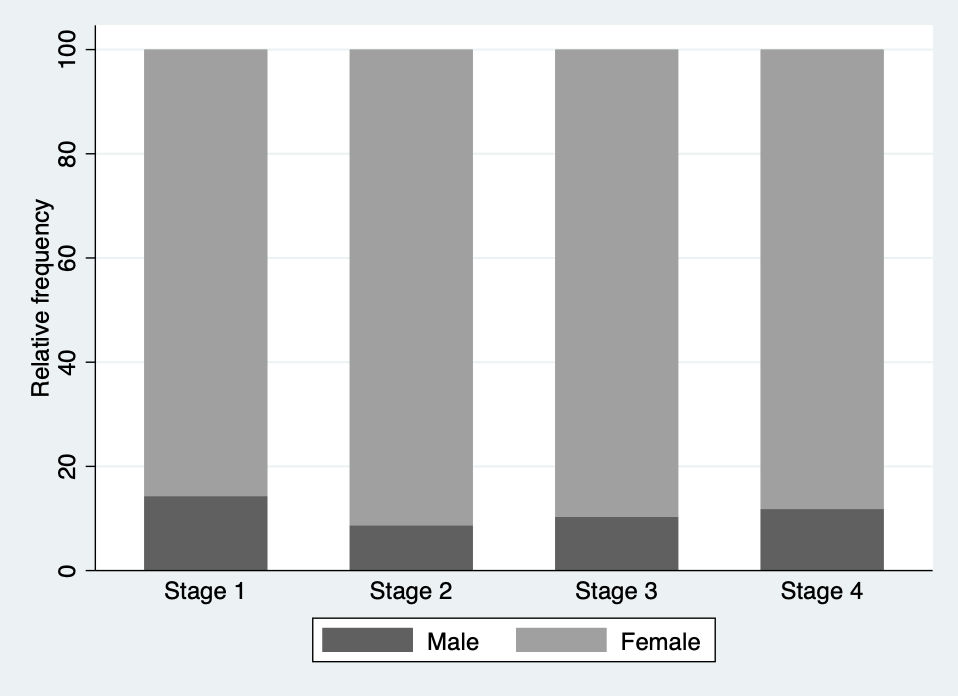
\includegraphics[width=0.75\linewidth]{img/mod01/stata/bar-12}

\hypertarget{editing-graphs-in-stata}{%
\subsection{Editing graphs in Stata}\label{editing-graphs-in-stata}}

There are two main approaches of editing many aspects of a graph (such as colours, labels, font-size etc). The first approach is to use options within the dialog boxes. For example, if we wanted to use a grey-and-white colour scheme for Figure X, we can define the colours of the bars in the Bars tab of the bar chart dialog box.

Here, we will define Bar 1 to be \texttt{White}:

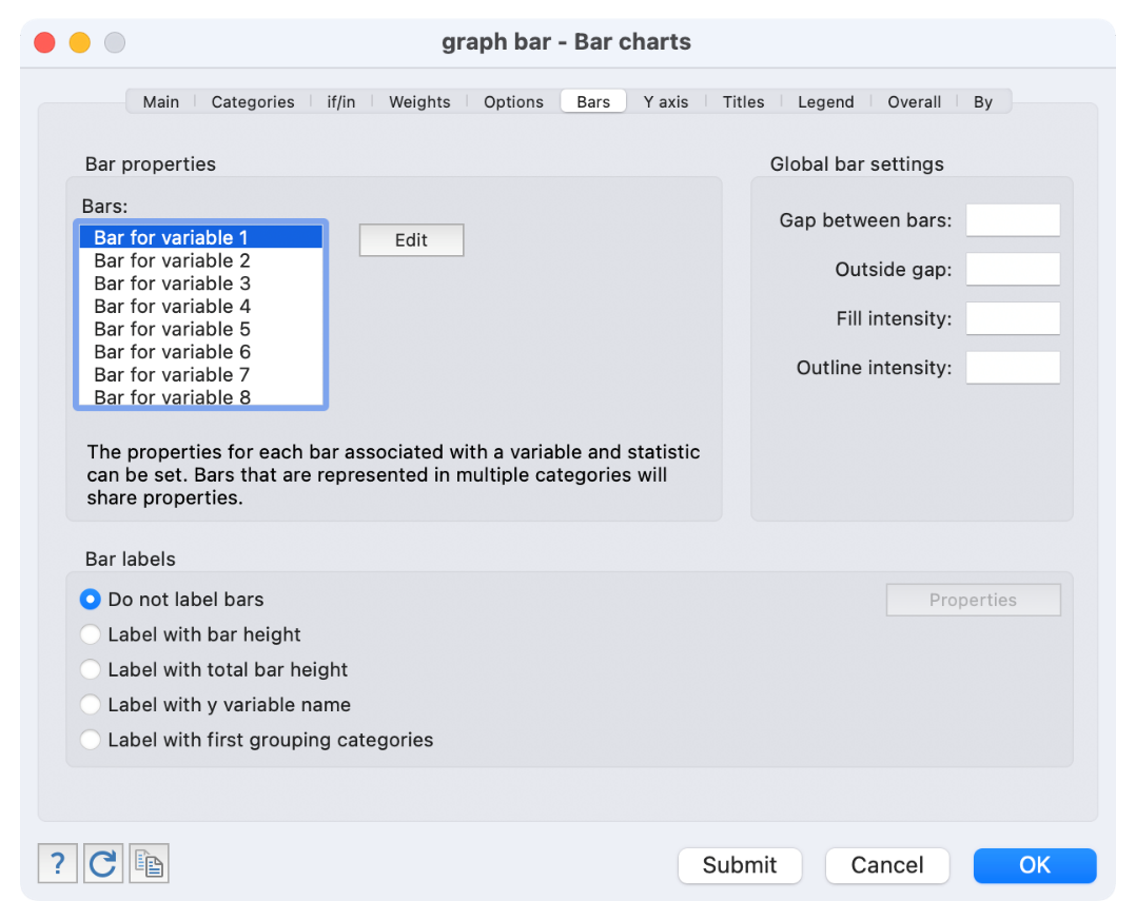
\includegraphics[width=0.75\linewidth]{img/mod01/stata/edit-01}

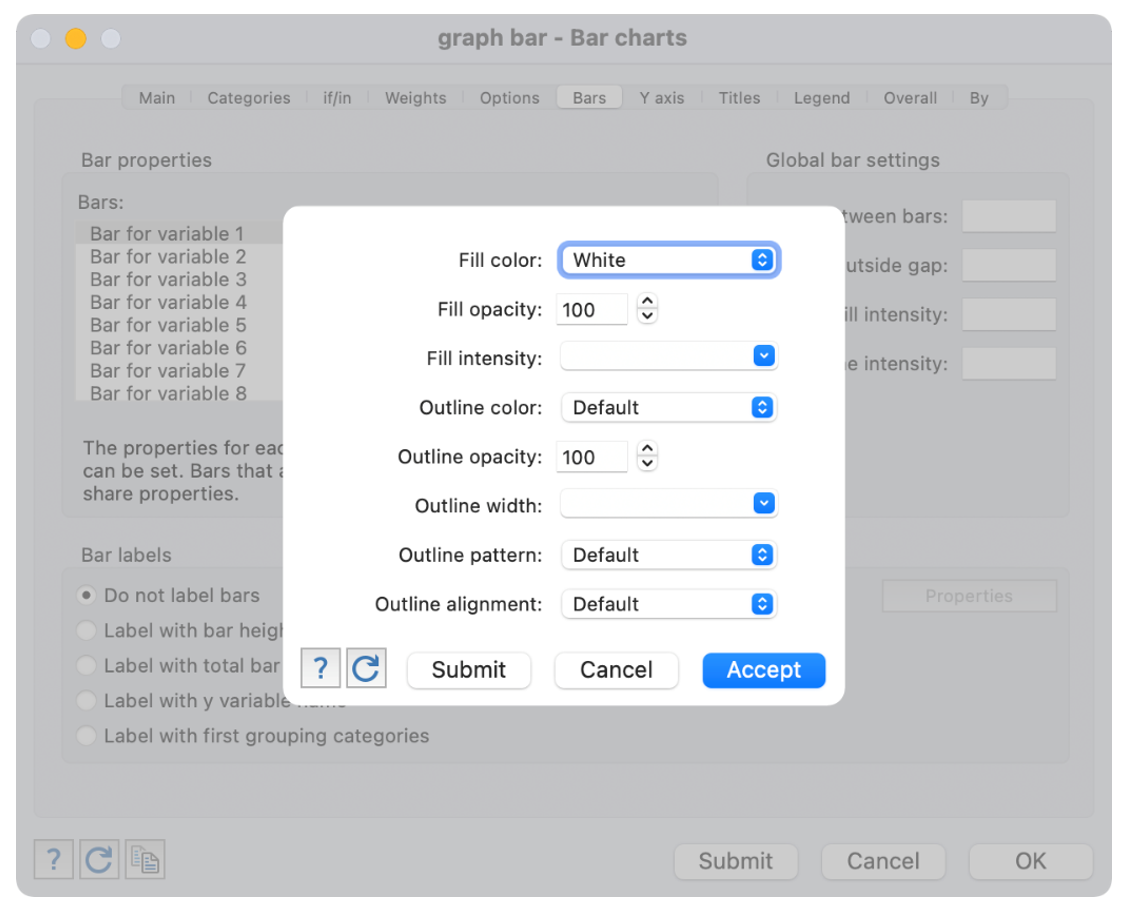
\includegraphics[width=0.75\linewidth]{img/mod01/stata/edit-02}

Bar 2 can be defined to be \texttt{Gray}, resulting in the graph below:

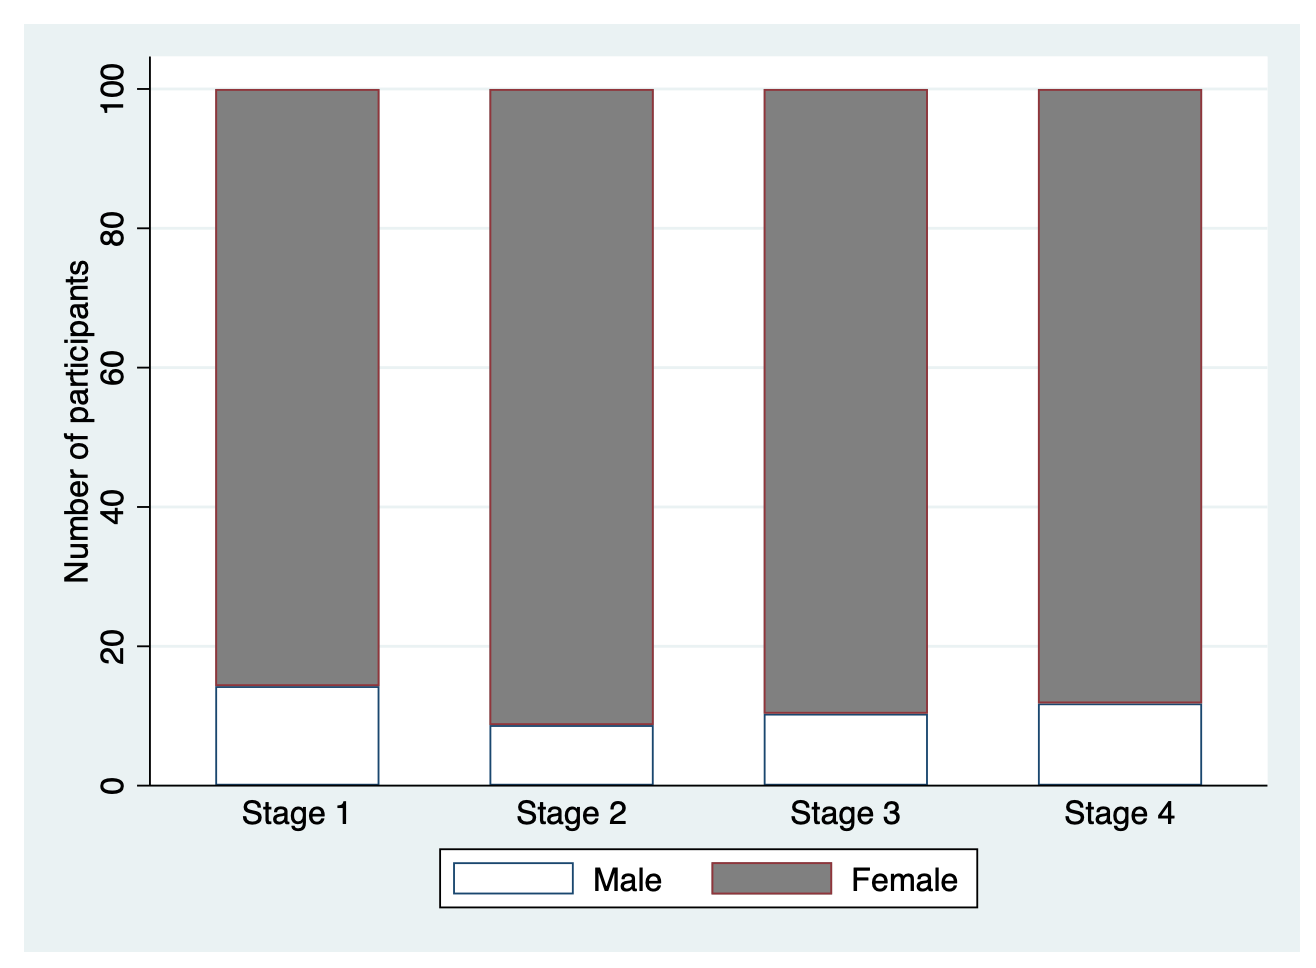
\includegraphics[width=0.75\linewidth]{img/mod01/stata/edit-03}

The second approach to customising graphs is to use the \textbf{Graph Editor}. Each Stata graph window includes a Graph Editor button:

\begin{figure}[H]
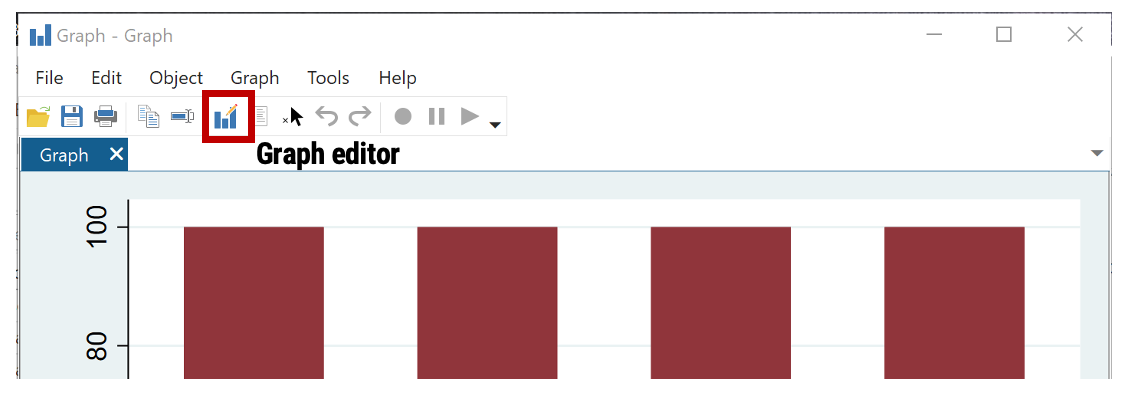
\includegraphics[width=0.75\linewidth]{img/mod01/stata/edit-04} \caption{Graph editor button on Stata for Windows}\label{fig:unnamed-chunk-44}
\end{figure}

\begin{figure}[H]
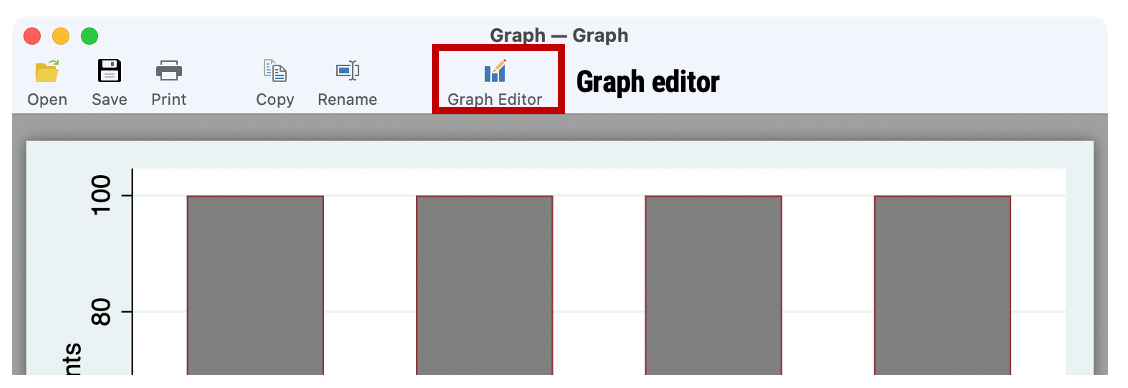
\includegraphics[width=0.75\linewidth]{img/mod01/stata/edit-05} \caption{Graph editor button on Stata for MacOS}\label{fig:unnamed-chunk-45}
\end{figure}

The \textbf{Graph Editor} window comprises two main sections: the graph that can be edited on the left, and a list of elements of the graph on the right. Most aspects of a graph's appearance can be edited in the Graph Editor, usually by double-clicking an element (e.g.~a bar, or a bar segment) and changing its properties. There are too many ways to change a graph's appearance to document here: feel free to explore and experiment!

\begin{figure}[H]
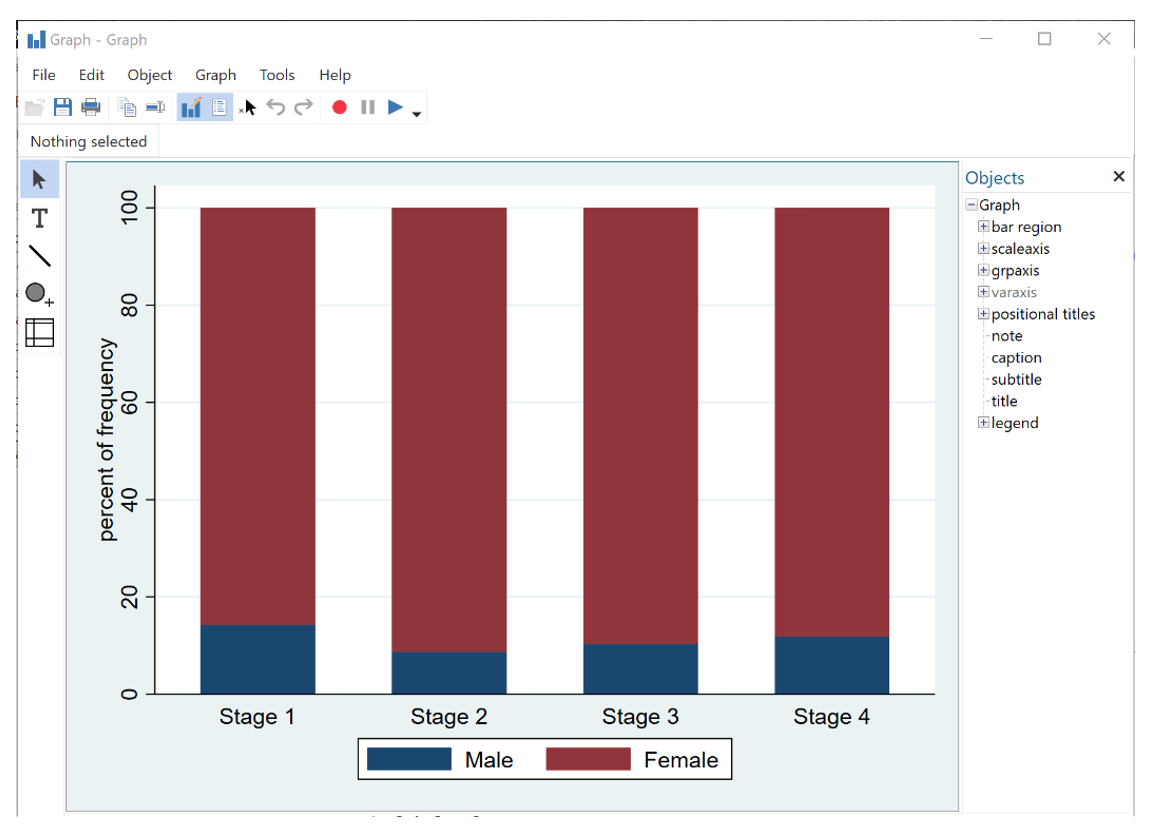
\includegraphics[width=0.75\linewidth]{img/mod01/stata/edit-06} \caption{Graph editor window: Windows}\label{fig:unnamed-chunk-46}
\end{figure}

\begin{figure}[H]
\includegraphics[width=0.75\linewidth]{img/mod01/stata/edit-07} \caption{Graph editor window: MacOS}\label{fig:unnamed-chunk-47}
\end{figure}

When you are done editing in the Graph Editor, click the Graph Editor icon again to stop the Graph Editor. You will be prompted to save your graph. You can click the \textbf{Save} button, choose \textbf{Save as} and choose to save using the \textbf{PNG (*.png)} format. You can then insert your saved PNG file into your word processing package as usual.

\hypertarget{creating-line-graphs}{%
\subsection{Creating line graphs}\label{creating-line-graphs}}

To demonstrate the graphing of aggregate data with Stata, we use the data on new cases and deaths from prostate cancer in males in NSW. This data has been entered into Stata as \texttt{Example\_1.2.dta}.

If you look at the data in the \textbf{Data Editor} window, you will see that there are 20 rows - a row for each year of data. Each row contains the number of new cases (\texttt{NCases}), number of deaths (\texttt{NDeaths}), the incidence rate (\texttt{RCases}) and death rate (\texttt{RDeaths}).

To create a line graph as in Figure \ref{fig:fig-1-5} select \textbf{Graphics \textgreater{} Twoway graph (scatter, line, etc.)} and click the \textbf{Create\ldots{}} button in the \textbf{twoway -- Twoway graphs} dialog box to bring up a dialog box for defining Plot 1.

\includegraphics[width=0.75\linewidth]{img/mod01/stata/line-01}

Choose \textbf{Line} as the plot type, \texttt{rcases} as the \textbf{Y variable} and \texttt{year} as the \textbf{X variable} as shown below.

\includegraphics[width=0.75\linewidth]{img/mod01/stata/line-02}

Click \textbf{Accept}, and then click \textbf{Submit} to check how the graph looks.

\includegraphics[width=0.75\linewidth]{img/mod01/stata/line-03}

This looks ok, but we want to add the death rate to the plot. Click \textbf{Create\ldots{}} again and add a Plot 2 for mortality rate:

\includegraphics[width=0.75\linewidth]{img/mod01/stata/line-03-1}

Choose \textbf{Line} as the plot type again, \texttt{rdeaths} as the \textbf{Y} variable and \texttt{year} as the \textbf{X variable}. Click \textbf{Accept}, and then \textbf{Submit} to check how the graph looks like now. You should see both variables plotted:

\includegraphics[width=0.75\linewidth]{img/mod01/stata/line-04}

To change the format of either line, click the relevant plot definition in the main \textbf{twoway} dialog box and click \textbf{Edit}. Click the \textbf{Line properties} button and choose a \textbf{Pattern} (e.g.~Short-dash), then click \textbf{Submit} again.

\includegraphics[width=0.75\linewidth]{img/mod01/stata/line-05}

\includegraphics[width=0.75\linewidth]{img/mod01/stata/line-06}

\includegraphics[width=0.75\linewidth]{img/mod01/stata/line-07}

\includegraphics[width=0.75\linewidth]{img/mod01/stata/line-08}

Next, we need an appropriate label for the y-axis. In the main \textbf{twoway} dialog box, click on the \textbf{Y axis} tab and label the title appropriately (e.g.~\texttt{Age-standardardised\ rate} and then click \textbf{OK} or \textbf{Submit}. The graph below should be produced.

\includegraphics[width=0.75\linewidth]{img/mod01/stata/line-09}

{[}Command: \texttt{twoway\ (line\ rcases\ year)\ (line\ rdeaths\ year,\ lpattern(shortdash)),\ ytitle(Age-standardised\ rate)}{]}

\hypertarget{learning-activities}{%
\chapter*{\texorpdfstring{\textbf{1} Learning Activities}{1 Learning Activities}}\label{learning-activities}}
\addcontentsline{toc}{chapter}{\textbf{1} Learning Activities}

\hypertarget{activity-1.1}{%
\subsection*{Activity 1.1}\label{activity-1.1}}
\addcontentsline{toc}{subsection}{Activity 1.1}

25 participants were enrolled in a 3-week weight loss programme. The following data present the weight loss (in grams) of the participants.

 
  \providecommand{\huxb}[2]{\arrayrulecolor[RGB]{#1}\global\arrayrulewidth=#2pt}
  \providecommand{\huxvb}[2]{\color[RGB]{#1}\vrule width #2pt}
  \providecommand{\huxtpad}[1]{\rule{0pt}{#1}}
  \providecommand{\huxbpad}[1]{\rule[-#1]{0pt}{#1}}

\begin{table}[ht]
\begin{centerbox}
\begin{threeparttable}
\captionsetup{justification=centering,singlelinecheck=off}
\caption{\label{tab:act-1-1} Weight loss (g) for 25 participants}
 \setlength{\tabcolsep}{0pt}
\begin{tabularx}{0.8\textwidth}{p{0.16\textwidth} p{0.16\textwidth} p{0.16\textwidth} p{0.16\textwidth} p{0.16\textwidth}}


\hhline{>{\huxb{0, 0, 0}{0.4}}->{\huxb{0, 0, 0}{0.4}}->{\huxb{0, 0, 0}{0.4}}->{\huxb{0, 0, 0}{0.4}}->{\huxb{0, 0, 0}{0.4}}-}
\arrayrulecolor{black}

\multicolumn{1}{!{\huxvb{0, 0, 0}{0}}p{0.16\textwidth}!{\huxvb{0, 0, 0}{0}}}{\hspace{0pt}\parbox[b]{0.16\textwidth-0pt-6pt}{\huxtpad{6pt + 1em}\raggedleft 255\huxbpad{6pt}}} &
\multicolumn{1}{p{0.16\textwidth}!{\huxvb{0, 0, 0}{0}}}{\hspace{6pt}\parbox[b]{0.16\textwidth-6pt-6pt}{\huxtpad{6pt + 1em}\raggedleft 198\huxbpad{6pt}}} &
\multicolumn{1}{p{0.16\textwidth}!{\huxvb{0, 0, 0}{0}}}{\hspace{6pt}\parbox[b]{0.16\textwidth-6pt-6pt}{\huxtpad{6pt + 1em}\raggedleft 283\huxbpad{6pt}}} &
\multicolumn{1}{p{0.16\textwidth}!{\huxvb{0, 0, 0}{0}}}{\hspace{6pt}\parbox[b]{0.16\textwidth-6pt-6pt}{\huxtpad{6pt + 1em}\raggedleft 312\huxbpad{6pt}}} &
\multicolumn{1}{p{0.16\textwidth}!{\huxvb{0, 0, 0}{0}}}{\hspace{6pt}\parbox[b]{0.16\textwidth-6pt-0pt}{\huxtpad{6pt + 1em}\raggedleft 283\huxbpad{6pt}}} \tabularnewline[-0.5pt]


\hhline{}
\arrayrulecolor{black}

\multicolumn{1}{!{\huxvb{0, 0, 0}{0}}p{0.16\textwidth}!{\huxvb{0, 0, 0}{0}}}{\hspace{0pt}\parbox[b]{0.16\textwidth-0pt-6pt}{\huxtpad{6pt + 1em}\raggedleft 57\huxbpad{6pt}}} &
\multicolumn{1}{p{0.16\textwidth}!{\huxvb{0, 0, 0}{0}}}{\hspace{6pt}\parbox[b]{0.16\textwidth-6pt-6pt}{\huxtpad{6pt + 1em}\raggedleft 85\huxbpad{6pt}}} &
\multicolumn{1}{p{0.16\textwidth}!{\huxvb{0, 0, 0}{0}}}{\hspace{6pt}\parbox[b]{0.16\textwidth-6pt-6pt}{\huxtpad{6pt + 1em}\raggedleft 312\huxbpad{6pt}}} &
\multicolumn{1}{p{0.16\textwidth}!{\huxvb{0, 0, 0}{0}}}{\hspace{6pt}\parbox[b]{0.16\textwidth-6pt-6pt}{\huxtpad{6pt + 1em}\raggedleft 142\huxbpad{6pt}}} &
\multicolumn{1}{p{0.16\textwidth}!{\huxvb{0, 0, 0}{0}}}{\hspace{6pt}\parbox[b]{0.16\textwidth-6pt-0pt}{\huxtpad{6pt + 1em}\raggedleft 113\huxbpad{6pt}}} \tabularnewline[-0.5pt]


\hhline{}
\arrayrulecolor{black}

\multicolumn{1}{!{\huxvb{0, 0, 0}{0}}p{0.16\textwidth}!{\huxvb{0, 0, 0}{0}}}{\hspace{0pt}\parbox[b]{0.16\textwidth-0pt-6pt}{\huxtpad{6pt + 1em}\raggedleft 227\huxbpad{6pt}}} &
\multicolumn{1}{p{0.16\textwidth}!{\huxvb{0, 0, 0}{0}}}{\hspace{6pt}\parbox[b]{0.16\textwidth-6pt-6pt}{\huxtpad{6pt + 1em}\raggedleft 283\huxbpad{6pt}}} &
\multicolumn{1}{p{0.16\textwidth}!{\huxvb{0, 0, 0}{0}}}{\hspace{6pt}\parbox[b]{0.16\textwidth-6pt-6pt}{\huxtpad{6pt + 1em}\raggedleft 255\huxbpad{6pt}}} &
\multicolumn{1}{p{0.16\textwidth}!{\huxvb{0, 0, 0}{0}}}{\hspace{6pt}\parbox[b]{0.16\textwidth-6pt-6pt}{\huxtpad{6pt + 1em}\raggedleft 340\huxbpad{6pt}}} &
\multicolumn{1}{p{0.16\textwidth}!{\huxvb{0, 0, 0}{0}}}{\hspace{6pt}\parbox[b]{0.16\textwidth-6pt-0pt}{\huxtpad{6pt + 1em}\raggedleft 142\huxbpad{6pt}}} \tabularnewline[-0.5pt]


\hhline{}
\arrayrulecolor{black}

\multicolumn{1}{!{\huxvb{0, 0, 0}{0}}p{0.16\textwidth}!{\huxvb{0, 0, 0}{0}}}{\hspace{0pt}\parbox[b]{0.16\textwidth-0pt-6pt}{\huxtpad{6pt + 1em}\raggedleft 113\huxbpad{6pt}}} &
\multicolumn{1}{p{0.16\textwidth}!{\huxvb{0, 0, 0}{0}}}{\hspace{6pt}\parbox[b]{0.16\textwidth-6pt-6pt}{\huxtpad{6pt + 1em}\raggedleft 312\huxbpad{6pt}}} &
\multicolumn{1}{p{0.16\textwidth}!{\huxvb{0, 0, 0}{0}}}{\hspace{6pt}\parbox[b]{0.16\textwidth-6pt-6pt}{\huxtpad{6pt + 1em}\raggedleft 227\huxbpad{6pt}}} &
\multicolumn{1}{p{0.16\textwidth}!{\huxvb{0, 0, 0}{0}}}{\hspace{6pt}\parbox[b]{0.16\textwidth-6pt-6pt}{\huxtpad{6pt + 1em}\raggedleft 85\huxbpad{6pt}}} &
\multicolumn{1}{p{0.16\textwidth}!{\huxvb{0, 0, 0}{0}}}{\hspace{6pt}\parbox[b]{0.16\textwidth-6pt-0pt}{\huxtpad{6pt + 1em}\raggedleft 170\huxbpad{6pt}}} \tabularnewline[-0.5pt]


\hhline{}
\arrayrulecolor{black}

\multicolumn{1}{!{\huxvb{0, 0, 0}{0}}p{0.16\textwidth}!{\huxvb{0, 0, 0}{0}}}{\hspace{0pt}\parbox[b]{0.16\textwidth-0pt-6pt}{\huxtpad{6pt + 1em}\raggedleft 255\huxbpad{6pt}}} &
\multicolumn{1}{p{0.16\textwidth}!{\huxvb{0, 0, 0}{0}}}{\hspace{6pt}\parbox[b]{0.16\textwidth-6pt-6pt}{\huxtpad{6pt + 1em}\raggedleft 198\huxbpad{6pt}}} &
\multicolumn{1}{p{0.16\textwidth}!{\huxvb{0, 0, 0}{0}}}{\hspace{6pt}\parbox[b]{0.16\textwidth-6pt-6pt}{\huxtpad{6pt + 1em}\raggedleft 113\huxbpad{6pt}}} &
\multicolumn{1}{p{0.16\textwidth}!{\huxvb{0, 0, 0}{0}}}{\hspace{6pt}\parbox[b]{0.16\textwidth-6pt-6pt}{\huxtpad{6pt + 1em}\raggedleft 227\huxbpad{6pt}}} &
\multicolumn{1}{p{0.16\textwidth}!{\huxvb{0, 0, 0}{0}}}{\hspace{6pt}\parbox[b]{0.16\textwidth-6pt-0pt}{\huxtpad{6pt + 1em}\raggedleft 255\huxbpad{6pt}}} \tabularnewline[-0.5pt]


\hhline{>{\huxb{0, 0, 0}{0.4}}->{\huxb{0, 0, 0}{0.4}}->{\huxb{0, 0, 0}{0.4}}->{\huxb{0, 0, 0}{0.4}}->{\huxb{0, 0, 0}{0.4}}-}
\arrayrulecolor{black}
\end{tabularx}
\end{threeparttable}\par\end{centerbox}

\end{table}
 

\begin{enumerate}
\def\labelenumi{\alph{enumi})}
\tightlist
\item
  Enter these data into Stata.
\item
  What type of data are these?
\item
  Construct an appropriate graph to display the relative frequency of participants' weight loss. Your graph should start at 50 grams, with weight loss grouped into 50 gram bins. Provide appropriate labels for the axes and give the graph an appropriate title.
\end{enumerate}

\hypertarget{activity-1.2}{%
\subsection*{Activity 1.2}\label{activity-1.2}}
\addcontentsline{toc}{subsection}{Activity 1.2}

Researchers at a maternity hospital in the 1970s conducted a study of low birth weight babies. Low birth weight is classified as a weight of 2,500g or less at birth. Data were collected on age and smoking status of mothers and the birth weight of their babies. The Stata file \texttt{Activity\_S1.2.dta} contains data on the participants in the study. The file is located on Moodle in the Learning Activities section.

Use Stata to create a 2 by 2 table to show the proportions of low birth weight babies born to mothers who smoked during pregnancy and those that did not smoke during pregnancy. Answer the following questions:

\begin{enumerate}
\def\labelenumi{\alph{enumi})}
\tightlist
\item
  What was the total number of mothers who smoked during pregnancy?
\item
  What proportion of mothers who smoked gave birth to low birth weight babies? What proportion of non-smoking mothers gave birth to low birth weight babies?
\item
  Use Stata to construct a stacked bar chart of the data to examine if there a difference in the proportion of babies born with a low birth weight in relation to the age group of the mother? Provide appropriate labels for the axes and give the graph an appropriate title. {[}Hint: plot the data using the \texttt{AgeGrp} variable{]}
\item
  Using your answers to the question a) and b), write a brief conclusion about the relationship of low birth weight and mother's age and smoking status.
\end{enumerate}

\hypertarget{activity-1.3}{%
\subsection*{Activity 1.3}\label{activity-1.3}}
\addcontentsline{toc}{subsection}{Activity 1.3}

Using Stata, estimate the mean, median, mode, standard deviation, range and interquartile range for the data Activity\_S1.3.dta, available on Moodle.

\hypertarget{activity-1.4}{%
\subsection*{Activity 1.4}\label{activity-1.4}}
\addcontentsline{toc}{subsection}{Activity 1.4}

Data of diastolic blood pressure (BP) of a sample of study participants are provided in the dataset Activity\_S1.4.dta. Compute the mean, median, range and SD of diastolic BP.

\hypertarget{activity-1.5}{%
\subsection*{Activity 1.5}\label{activity-1.5}}
\addcontentsline{toc}{subsection}{Activity 1.5}

In a study of 100 participants data were missing for 5 people. The missing data points were coded as `99'. The mean of the data was estimated as 45.0 with a standard deviation of 5.6; the smallest and greatest values are 16 and 65 respectively.

If the researcher analysed the data as if the 99s were real data, would it make the following statistics larger, smaller, or stay the same?

\begin{enumerate}
\def\labelenumi{\alph{enumi})}
\tightlist
\item
  Mean
\item
  Standard Deviation
\item
  Range
\end{enumerate}

\hypertarget{activity-1.6}{%
\subsection*{Activity 1.6}\label{activity-1.6}}
\addcontentsline{toc}{subsection}{Activity 1.6}

Which of the following statements are true? The more dispersed, or spread out, a set of observations are:

\begin{enumerate}
\def\labelenumi{\alph{enumi})}
\tightlist
\item
  The smaller the mean value
\item
  The larger the standard deviation
\item
  The smaller the variance
\end{enumerate}

\hypertarget{activity-1.7}{%
\subsection*{Activity 1.7}\label{activity-1.7}}
\addcontentsline{toc}{subsection}{Activity 1.7}

If the variance for a set of scores is equal to 9, what is the standard deviation?

\hypertarget{probability-and-probability-distributions}{%
\chapter{Probability and probability distributions}\label{probability-and-probability-distributions}}

\hypertarget{learning-objectives-1}{%
\section*{Learning objectives}\label{learning-objectives-1}}
\addcontentsline{toc}{section}{Learning objectives}

By the end of this module you will be able to:

\begin{itemize}
\tightlist
\item
  Describe the concept of probability;
\item
  Describe the characteristics of a binomial distribution and a Normal distribution;
\item
  Compute binomial probabilities using Stata;
\item
  Compute and use Z-scores to obtain probabilities;
\item
  Decide when to use parametric or non-parametric statistical methods;
\item
  Briefly outline other types of distributions.
\end{itemize}

\hypertarget{readings-1}{%
\section*{Readings}\label{readings-1}}
\addcontentsline{toc}{section}{Readings}

\citet{kirkwood_sterne01}; Chapters 5, 14 and 15. \href{http://er1.library.unsw.edu.au/er/cgi-bin/eraccess.cgi?url=https://ebookcentral.proquest.com/lib/unsw/detail.action?docID=624728}{{[}UNSW Library Link{]}}

\citet{bland15}; Chapters 6 and 7. \href{http://er1.library.unsw.edu.au/er/cgi-bin/eraccess.cgi?url=https://ebookcentral.proquest.com/lib/unsw/detail.action?docID=5891730}{{[}UNSW Library Link{]}}

\hypertarget{introduction-1}{%
\section{Introduction}\label{introduction-1}}

In Module 1, we looked at how to summarise data numerically and graphically. In this module, we will introduce the concept of probability which underpins the theoretical basis of statistics, and then introduce the concept of probability distributions. We will look at the binomial distribution, and then look at the most important distribution in statistics: the Normal distribution. Finally, we introduce some other probability distributions commonly used in biostatistics.

\hypertarget{probability}{%
\section{Probability}\label{probability}}

Probability is defined as:

\begin{quote}
the chance of an event occurring, where an event is the result of an observation or experiment, or the description of some potential outcome.
\end{quote}

Probabilities range from 0 (where the event will never occur) to 1 (where the event will always occur). For example, tossing a coin is an experiment; one event is the coin landing with head up, while the other event is the coin landing tails up. The set of all possible outcomes in an experiment is called the sample space. For example, by tossing a coin you can get either a head or a tail (called mutually exclusive events); and by rolling a die you can get any of the six sides. Thus, for a die the sampling space is: S = \{1, 2, 3, 4, 5, 6\}

With a fair (unbiased) die, the probability of each outcome occurring is 1/6 and its probability distribution is simply a probability of 1/6 for each of the six numbers on a die.

\hypertarget{additive-law-of-probability}{%
\subsection{Additive law of probability}\label{additive-law-of-probability}}

How do we work out the probability that one roll of a die will turn out to be a 3 or a 6? To do that, we first need to work out whether the events (3 or 6 on the roll of a die) are mutually exclusive. Events are mutually exclusive if they are events which cannot occur at the same time. For example, rolling a die once and getting a 3 and 6 are mutually exclusive events (you can roll one or the other but not both in a single roll).

To obtain the probability of one or the other of two mutually exclusive events occurring, the sum of the probabilities of each is taken. For example, the probability of the roll of a die being a 3 or a 6 is the sum of the probability of the die being 3 (i.e.~1/6) and the probability of the die being 6 (also 1/6). With a fair die:

Probability of a die roll being 3 or 6 = \(1/6 + 1/6 = 1/3\)

Another way of putting it is:

P(die roll =3 or die roll =6) = P(die roll=3) + P(die roll=6) = \(1/6 + 1/6 = 1/3\)

\hypertarget{example-additive-law-for-mutually-exclusive-events}{%
\subsubsection*{Example: Additive law for mutually exclusive events}\label{example-additive-law-for-mutually-exclusive-events}}
\addcontentsline{toc}{subsubsection}{Example: Additive law for mutually exclusive events}

Consider that blood type can be organised into the ABO system (blood types A, B, AB or O) An individual may only have one blood type.

Using the information from \url{https://www.donateblood.com.au/learn/about-blood} let's consider the ABO blood type system. The frequency distribution (prevalence) of the ABO blood type system in the population represents the probability of each of the outcomes. If we consider all possible blood type outcomes, then the total of the probabilities will sum to 1 (100\%).

 
  \providecommand{\huxb}[2]{\arrayrulecolor[RGB]{#1}\global\arrayrulewidth=#2pt}
  \providecommand{\huxvb}[2]{\color[RGB]{#1}\vrule width #2pt}
  \providecommand{\huxtpad}[1]{\rule{0pt}{#1}}
  \providecommand{\huxbpad}[1]{\rule[-#1]{0pt}{#1}}

\begin{table}[ht]
\begin{centerbox}
\begin{threeparttable}
\captionsetup{justification=centering,singlelinecheck=off}
\caption{\label{tab:tab-2-1} Frequency of blood types}
 \setlength{\tabcolsep}{0pt}
\begin{tabularx}{0.6\textwidth}{p{0.2\textwidth} p{0.2\textwidth} p{0.2\textwidth}}


\hhline{>{\huxb{0, 0, 0}{0.4}}->{\huxb{0, 0, 0}{0.4}}->{\huxb{0, 0, 0}{0.4}}-}
\arrayrulecolor{black}

\multicolumn{1}{!{\huxvb{0, 0, 0}{0}}p{0.2\textwidth}!{\huxvb{0, 0, 0}{0}}}{\hspace{0pt}\parbox[b]{0.2\textwidth-0pt-6pt}{\huxtpad{6pt + 1em}\raggedleft \textbf{Blood Type}\huxbpad{6pt}}} &
\multicolumn{1}{p{0.2\textwidth}!{\huxvb{0, 0, 0}{0}}}{\hspace{6pt}\parbox[b]{0.2\textwidth-6pt-6pt}{\huxtpad{6pt + 1em}\raggedleft \textbf{\% of population}\huxbpad{6pt}}} &
\multicolumn{1}{p{0.2\textwidth}!{\huxvb{0, 0, 0}{0}}}{\hspace{6pt}\parbox[b]{0.2\textwidth-6pt-0pt}{\huxtpad{6pt + 1em}\raggedleft \textbf{Probability\hphantom{0}\hphantom{0}\hphantom{0}}\huxbpad{6pt}}} \tabularnewline[-0.5pt]


\hhline{>{\huxb{0, 0, 0}{0.4}}->{\huxb{0, 0, 0}{0.4}}->{\huxb{0, 0, 0}{0.4}}-}
\arrayrulecolor{black}

\multicolumn{1}{!{\huxvb{0, 0, 0}{0}}p{0.2\textwidth}!{\huxvb{0, 0, 0}{0}}}{\hspace{0pt}\parbox[b]{0.2\textwidth-0pt-6pt}{\huxtpad{6pt + 1em}\raggedleft A\huxbpad{6pt}}} &
\multicolumn{1}{p{0.2\textwidth}!{\huxvb{0, 0, 0}{0}}}{\hspace{6pt}\parbox[b]{0.2\textwidth-6pt-6pt}{\huxtpad{6pt + 1em}\raggedleft 38\%\huxbpad{6pt}}} &
\multicolumn{1}{p{0.2\textwidth}!{\huxvb{0, 0, 0}{0}}}{\hspace{6pt}\parbox[b]{0.2\textwidth-6pt-0pt}{\huxtpad{6pt + 1em}\raggedleft 0.38\huxbpad{6pt}}} \tabularnewline[-0.5pt]


\hhline{}
\arrayrulecolor{black}

\multicolumn{1}{!{\huxvb{0, 0, 0}{0}}p{0.2\textwidth}!{\huxvb{0, 0, 0}{0}}}{\hspace{0pt}\parbox[b]{0.2\textwidth-0pt-6pt}{\huxtpad{6pt + 1em}\raggedleft B\huxbpad{6pt}}} &
\multicolumn{1}{p{0.2\textwidth}!{\huxvb{0, 0, 0}{0}}}{\hspace{6pt}\parbox[b]{0.2\textwidth-6pt-6pt}{\huxtpad{6pt + 1em}\raggedleft 10\%\huxbpad{6pt}}} &
\multicolumn{1}{p{0.2\textwidth}!{\huxvb{0, 0, 0}{0}}}{\hspace{6pt}\parbox[b]{0.2\textwidth-6pt-0pt}{\huxtpad{6pt + 1em}\raggedleft 0.1\hphantom{0}\huxbpad{6pt}}} \tabularnewline[-0.5pt]


\hhline{}
\arrayrulecolor{black}

\multicolumn{1}{!{\huxvb{0, 0, 0}{0}}p{0.2\textwidth}!{\huxvb{0, 0, 0}{0}}}{\hspace{0pt}\parbox[b]{0.2\textwidth-0pt-6pt}{\huxtpad{6pt + 1em}\raggedleft AB\huxbpad{6pt}}} &
\multicolumn{1}{p{0.2\textwidth}!{\huxvb{0, 0, 0}{0}}}{\hspace{6pt}\parbox[b]{0.2\textwidth-6pt-6pt}{\huxtpad{6pt + 1em}\raggedleft 3\%\huxbpad{6pt}}} &
\multicolumn{1}{p{0.2\textwidth}!{\huxvb{0, 0, 0}{0}}}{\hspace{6pt}\parbox[b]{0.2\textwidth-6pt-0pt}{\huxtpad{6pt + 1em}\raggedleft 0.03\huxbpad{6pt}}} \tabularnewline[-0.5pt]


\hhline{}
\arrayrulecolor{black}

\multicolumn{1}{!{\huxvb{0, 0, 0}{0}}p{0.2\textwidth}!{\huxvb{0, 0, 0}{0}}}{\hspace{0pt}\parbox[b]{0.2\textwidth-0pt-6pt}{\huxtpad{6pt + 1em}\raggedleft O\huxbpad{6pt}}} &
\multicolumn{1}{p{0.2\textwidth}!{\huxvb{0, 0, 0}{0}}}{\hspace{6pt}\parbox[b]{0.2\textwidth-6pt-6pt}{\huxtpad{6pt + 1em}\raggedleft 49\%\huxbpad{6pt}}} &
\multicolumn{1}{p{0.2\textwidth}!{\huxvb{0, 0, 0}{0}}}{\hspace{6pt}\parbox[b]{0.2\textwidth-6pt-0pt}{\huxtpad{6pt + 1em}\raggedleft 0.49\huxbpad{6pt}}} \tabularnewline[-0.5pt]


\hhline{}
\arrayrulecolor{black}

\multicolumn{1}{!{\huxvb{0, 0, 0}{0}}p{0.2\textwidth}!{\huxvb{0, 0, 0}{0}}}{\hspace{0pt}\parbox[b]{0.2\textwidth-0pt-6pt}{\huxtpad{6pt + 1em}\raggedleft Total\huxbpad{6pt}}} &
\multicolumn{1}{p{0.2\textwidth}!{\huxvb{0, 0, 0}{0}}}{\hspace{6pt}\parbox[b]{0.2\textwidth-6pt-6pt}{\huxtpad{6pt + 1em}\raggedleft 100\%\huxbpad{6pt}}} &
\multicolumn{1}{p{0.2\textwidth}!{\huxvb{0, 0, 0}{0}}}{\hspace{6pt}\parbox[b]{0.2\textwidth-6pt-0pt}{\huxtpad{6pt + 1em}\raggedleft 1\hphantom{0}\hphantom{0}\hphantom{0}\huxbpad{6pt}}} \tabularnewline[-0.5pt]


\hhline{>{\huxb{0, 0, 0}{0.4}}->{\huxb{0, 0, 0}{0.4}}->{\huxb{0, 0, 0}{0.4}}-}
\arrayrulecolor{black}
\end{tabularx}
\end{threeparttable}\par\end{centerbox}

\end{table}
 

In this example we consider: What is the probability that an individual will have either blood group O or A?

Since blood type is mutually exclusive, the probability that either one or the other occurs is the sum of the individual probabilities. These are mutually exclusive events so we can say P(O or A) = P(O) + P(A)

Thus, the answer is: P(Blood type O) + P(Blood type A) = 0.49 + 0.38 = 0.87

\hypertarget{multiplicative-law-of-probability}{%
\subsection{Multiplicative law of probability}\label{multiplicative-law-of-probability}}

The additive law of probability lets us consider the probability of different outcomes in a single experiment. The multiplicative law lets us consider the probability of multiple events occurring in a particular order. For example: if I roll a die twice, what is the probability of rolling a 3 and \emph{then} a 6?

These events are independent: the probability of rolling a 6 on the second roll is not affected by the first roll.

The multiplicative law of probability states:

\begin{quote}
If A and B are independent, then P(A and B) = P(A) \(\times\) P(B).
\end{quote}

So, the probability of rolling a 3 and then a 6 is: P(3 and 6) = \(1/6 \times 1/6 = 1/36\).

Note here that the order matters -- we are considering the probability of rolling a 3 and then a 6, not the probability of rolling a 6 and then a 3.

\hypertarget{probability-distributions}{%
\section{Probability distributions}\label{probability-distributions}}

A probability distribution is a table or a function that provides the probabilities of all possible outcomes for a random variable (a variable whose outcome depends on a random process). For example, the probability distribution for a single coin toss is straightforward: the probability of obtaining a head is 0.5, and the probability of obtaining a tail is 0.5. Similarly, the probability distribution for a single roll of a die is straightforward: each face has a probability of 1/6.

 
  \providecommand{\huxb}[2]{\arrayrulecolor[RGB]{#1}\global\arrayrulewidth=#2pt}
  \providecommand{\huxvb}[2]{\color[RGB]{#1}\vrule width #2pt}
  \providecommand{\huxtpad}[1]{\rule{0pt}{#1}}
  \providecommand{\huxbpad}[1]{\rule[-#1]{0pt}{#1}}

\begin{table}[ht]
\begin{centerbox}
\begin{threeparttable}
\captionsetup{justification=centering,singlelinecheck=off}
\caption{\label{tab:tab-2-2} Probability distributions for (a) a single coin toss and (b) a single roll of a die}
 \setlength{\tabcolsep}{0pt}
\begin{tabularx}{0.95\textwidth}{p{0.19\textwidth} p{0.19\textwidth} p{0.19\textwidth} p{0.19\textwidth} p{0.19\textwidth}}


\hhline{>{\huxb{0, 0, 0}{0.4}}->{\huxb{0, 0, 0}{0.4}}->{\huxb{0, 0, 0}{0.4}}->{\huxb{0, 0, 0}{0.4}}->{\huxb{0, 0, 0}{0.4}}-}
\arrayrulecolor{black}

\multicolumn{1}{!{\huxvb{0, 0, 0}{0}}p{0.19\textwidth}!{\huxvb{0, 0, 0}{0}}}{\hspace{0pt}\parbox[b]{0.19\textwidth-0pt-6pt}{\huxtpad{6pt + 1em}\centering \textbf{Coin face}\huxbpad{6pt}}} &
\multicolumn{1}{p{0.19\textwidth}!{\huxvb{0, 0, 0}{0}}}{\hspace{6pt}\parbox[b]{0.19\textwidth-6pt-6pt}{\huxtpad{6pt + 1em}\centering \textbf{Probability}\huxbpad{6pt}}} &
\multicolumn{1}{p{0.19\textwidth}!{\huxvb{0, 0, 0}{0}}}{\hspace{6pt}\parbox[b]{0.19\textwidth-6pt-6pt}{\huxtpad{6pt + 1em}\centering \textbf{ }\huxbpad{6pt}}} &
\multicolumn{1}{p{0.19\textwidth}!{\huxvb{0, 0, 0}{0}}}{\hspace{6pt}\parbox[b]{0.19\textwidth-6pt-6pt}{\huxtpad{6pt + 1em}\centering \textbf{Face of a die}\huxbpad{6pt}}} &
\multicolumn{1}{p{0.19\textwidth}!{\huxvb{0, 0, 0}{0}}}{\hspace{6pt}\parbox[b]{0.19\textwidth-6pt-0pt}{\huxtpad{6pt + 1em}\centering \textbf{Probability}\huxbpad{6pt}}} \tabularnewline[-0.5pt]


\hhline{>{\huxb{0, 0, 0}{0.4}}->{\huxb{0, 0, 0}{0.4}}->{\huxb{0, 0, 0}{0.4}}->{\huxb{0, 0, 0}{0.4}}->{\huxb{0, 0, 0}{0.4}}-}
\arrayrulecolor{black}

\multicolumn{1}{!{\huxvb{0, 0, 0}{0}}p{0.19\textwidth}!{\huxvb{0, 0, 0}{0}}}{\hspace{0pt}\parbox[b]{0.19\textwidth-0pt-6pt}{\huxtpad{6pt + 1em}\centering Heads\huxbpad{6pt}}} &
\multicolumn{1}{p{0.19\textwidth}!{\huxvb{0, 0, 0}{0}}}{\hspace{6pt}\parbox[b]{0.19\textwidth-6pt-6pt}{\huxtpad{6pt + 1em}\centering 0.5\huxbpad{6pt}}} &
\multicolumn{1}{p{0.19\textwidth}!{\huxvb{0, 0, 0}{0}}}{\hspace{6pt}\parbox[b]{0.19\textwidth-6pt-6pt}{\huxtpad{6pt + 1em}\centering \huxbpad{6pt}}} &
\multicolumn{1}{p{0.19\textwidth}!{\huxvb{0, 0, 0}{0}}}{\hspace{6pt}\parbox[b]{0.19\textwidth-6pt-6pt}{\huxtpad{6pt + 1em}\centering 1\huxbpad{6pt}}} &
\multicolumn{1}{p{0.19\textwidth}!{\huxvb{0, 0, 0}{0}}}{\hspace{6pt}\parbox[b]{0.19\textwidth-6pt-0pt}{\huxtpad{6pt + 1em}\centering 1/6\huxbpad{6pt}}} \tabularnewline[-0.5pt]


\hhline{}
\arrayrulecolor{black}

\multicolumn{1}{!{\huxvb{0, 0, 0}{0}}p{0.19\textwidth}!{\huxvb{0, 0, 0}{0}}}{\hspace{0pt}\parbox[b]{0.19\textwidth-0pt-6pt}{\huxtpad{6pt + 1em}\centering Tails\huxbpad{6pt}}} &
\multicolumn{1}{p{0.19\textwidth}!{\huxvb{0, 0, 0}{0}}}{\hspace{6pt}\parbox[b]{0.19\textwidth-6pt-6pt}{\huxtpad{6pt + 1em}\centering 0.5\huxbpad{6pt}}} &
\multicolumn{1}{p{0.19\textwidth}!{\huxvb{0, 0, 0}{0}}}{\hspace{6pt}\parbox[b]{0.19\textwidth-6pt-6pt}{\huxtpad{6pt + 1em}\centering \huxbpad{6pt}}} &
\multicolumn{1}{p{0.19\textwidth}!{\huxvb{0, 0, 0}{0}}}{\hspace{6pt}\parbox[b]{0.19\textwidth-6pt-6pt}{\huxtpad{6pt + 1em}\centering 2\huxbpad{6pt}}} &
\multicolumn{1}{p{0.19\textwidth}!{\huxvb{0, 0, 0}{0}}}{\hspace{6pt}\parbox[b]{0.19\textwidth-6pt-0pt}{\huxtpad{6pt + 1em}\centering 1/6\huxbpad{6pt}}} \tabularnewline[-0.5pt]


\hhline{}
\arrayrulecolor{black}

\multicolumn{1}{!{\huxvb{0, 0, 0}{0}}p{0.19\textwidth}!{\huxvb{0, 0, 0}{0}}}{\hspace{0pt}\parbox[b]{0.19\textwidth-0pt-6pt}{\huxtpad{6pt + 1em}\centering \huxbpad{6pt}}} &
\multicolumn{1}{p{0.19\textwidth}!{\huxvb{0, 0, 0}{0}}}{\hspace{6pt}\parbox[b]{0.19\textwidth-6pt-6pt}{\huxtpad{6pt + 1em}\centering \huxbpad{6pt}}} &
\multicolumn{1}{p{0.19\textwidth}!{\huxvb{0, 0, 0}{0}}}{\hspace{6pt}\parbox[b]{0.19\textwidth-6pt-6pt}{\huxtpad{6pt + 1em}\centering \huxbpad{6pt}}} &
\multicolumn{1}{p{0.19\textwidth}!{\huxvb{0, 0, 0}{0}}}{\hspace{6pt}\parbox[b]{0.19\textwidth-6pt-6pt}{\huxtpad{6pt + 1em}\centering 3\huxbpad{6pt}}} &
\multicolumn{1}{p{0.19\textwidth}!{\huxvb{0, 0, 0}{0}}}{\hspace{6pt}\parbox[b]{0.19\textwidth-6pt-0pt}{\huxtpad{6pt + 1em}\centering 1/6\huxbpad{6pt}}} \tabularnewline[-0.5pt]


\hhline{}
\arrayrulecolor{black}

\multicolumn{1}{!{\huxvb{0, 0, 0}{0}}p{0.19\textwidth}!{\huxvb{0, 0, 0}{0}}}{\hspace{0pt}\parbox[b]{0.19\textwidth-0pt-6pt}{\huxtpad{6pt + 1em}\centering \huxbpad{6pt}}} &
\multicolumn{1}{p{0.19\textwidth}!{\huxvb{0, 0, 0}{0}}}{\hspace{6pt}\parbox[b]{0.19\textwidth-6pt-6pt}{\huxtpad{6pt + 1em}\centering \huxbpad{6pt}}} &
\multicolumn{1}{p{0.19\textwidth}!{\huxvb{0, 0, 0}{0}}}{\hspace{6pt}\parbox[b]{0.19\textwidth-6pt-6pt}{\huxtpad{6pt + 1em}\centering \huxbpad{6pt}}} &
\multicolumn{1}{p{0.19\textwidth}!{\huxvb{0, 0, 0}{0}}}{\hspace{6pt}\parbox[b]{0.19\textwidth-6pt-6pt}{\huxtpad{6pt + 1em}\centering 4\huxbpad{6pt}}} &
\multicolumn{1}{p{0.19\textwidth}!{\huxvb{0, 0, 0}{0}}}{\hspace{6pt}\parbox[b]{0.19\textwidth-6pt-0pt}{\huxtpad{6pt + 1em}\centering 1/6\huxbpad{6pt}}} \tabularnewline[-0.5pt]


\hhline{}
\arrayrulecolor{black}

\multicolumn{1}{!{\huxvb{0, 0, 0}{0}}p{0.19\textwidth}!{\huxvb{0, 0, 0}{0}}}{\hspace{0pt}\parbox[b]{0.19\textwidth-0pt-6pt}{\huxtpad{6pt + 1em}\centering \huxbpad{6pt}}} &
\multicolumn{1}{p{0.19\textwidth}!{\huxvb{0, 0, 0}{0}}}{\hspace{6pt}\parbox[b]{0.19\textwidth-6pt-6pt}{\huxtpad{6pt + 1em}\centering \huxbpad{6pt}}} &
\multicolumn{1}{p{0.19\textwidth}!{\huxvb{0, 0, 0}{0}}}{\hspace{6pt}\parbox[b]{0.19\textwidth-6pt-6pt}{\huxtpad{6pt + 1em}\centering \huxbpad{6pt}}} &
\multicolumn{1}{p{0.19\textwidth}!{\huxvb{0, 0, 0}{0}}}{\hspace{6pt}\parbox[b]{0.19\textwidth-6pt-6pt}{\huxtpad{6pt + 1em}\centering 5\huxbpad{6pt}}} &
\multicolumn{1}{p{0.19\textwidth}!{\huxvb{0, 0, 0}{0}}}{\hspace{6pt}\parbox[b]{0.19\textwidth-6pt-0pt}{\huxtpad{6pt + 1em}\centering 1/6\huxbpad{6pt}}} \tabularnewline[-0.5pt]


\hhline{}
\arrayrulecolor{black}

\multicolumn{1}{!{\huxvb{0, 0, 0}{0}}p{0.19\textwidth}!{\huxvb{0, 0, 0}{0}}}{\hspace{0pt}\parbox[b]{0.19\textwidth-0pt-6pt}{\huxtpad{6pt + 1em}\centering \huxbpad{6pt}}} &
\multicolumn{1}{p{0.19\textwidth}!{\huxvb{0, 0, 0}{0}}}{\hspace{6pt}\parbox[b]{0.19\textwidth-6pt-6pt}{\huxtpad{6pt + 1em}\centering \huxbpad{6pt}}} &
\multicolumn{1}{p{0.19\textwidth}!{\huxvb{0, 0, 0}{0}}}{\hspace{6pt}\parbox[b]{0.19\textwidth-6pt-6pt}{\huxtpad{6pt + 1em}\centering \huxbpad{6pt}}} &
\multicolumn{1}{p{0.19\textwidth}!{\huxvb{0, 0, 0}{0}}}{\hspace{6pt}\parbox[b]{0.19\textwidth-6pt-6pt}{\huxtpad{6pt + 1em}\centering 6\huxbpad{6pt}}} &
\multicolumn{1}{p{0.19\textwidth}!{\huxvb{0, 0, 0}{0}}}{\hspace{6pt}\parbox[b]{0.19\textwidth-6pt-0pt}{\huxtpad{6pt + 1em}\centering 1/6\huxbpad{6pt}}} \tabularnewline[-0.5pt]


\hhline{>{\huxb{0, 0, 0}{0.4}}->{\huxb{0, 0, 0}{0.4}}->{\huxb{0, 0, 0}{0.4}}->{\huxb{0, 0, 0}{0.4}}->{\huxb{0, 0, 0}{0.4}}-}
\arrayrulecolor{black}
\end{tabularx}
\end{threeparttable}\par\end{centerbox}

\end{table}
 

Things become more complicated when we consider a series of coin-tosses, or rolls of a die. These series of events can be summarised by considering the number of times a certain outcome is observed. For example, the probability of obtaining three heads from five coin tosses.

Probability distributions can be used in two main ways:
1. To calculate the probability of an event occurring. This seems trivial for the coin-toss and die-roll examples above. However, we can consider more complex events, as below.
1. To understand the behaviour of a sample statistic. We will see in Modules 3 and 4 that the mean of a sample follows a probability distribution. We can obtain useful information about a sample mean by using properties of the probability distribution.

\hypertarget{discrete-variables-and-their-probability-distributions}{%
\section{Discrete variables and their probability distributions}\label{discrete-variables-and-their-probability-distributions}}

A discrete random variable is a random variable that has countable values (non-negative integers). An example of a discrete random variable is the number of heads observed in a series of coin tosses.

A discrete random variable can be summarised by listing all the possible values that the variable can take. As defined earlier, a table, formula or graph that presents these possible values, and their associated probabilities, is called a probability distribution.

Example: let's consider the number of heads in a series of three coin tosses. We might observe 0 heads, or 1 head, or 2, or 3 heads. If we let X denote the number of heads in a series of three coin tosses, then possible values of X are 0, 1, 2 or 3.

We write the probability of observing x heads as P(X=x). So P(X=0) is the probability that the three tosses has no heads. Similarly, P(X=1) is the probability of observing one head.
The possible combinations for three coin tosses are as follows:

There are eight possible outcomes from three coin tosses (permutations). If we assume an equal chance of observing a head or a tail, each permutation above is equally likely, and so has a probability of 1/8.

However, if we consider the possibility of observing just one head out of the three tosses, this can happen in three ways (HTT, THT, TTH). So the probability of observing one head is calculated using the additive law: P(X=1) = \(\tfrac{1}{8} + \tfrac{1}{8} + \tfrac{1}{8} = \tfrac{3}{8}\).

Therefore, the probability distribution for X, the number of heads from three coin tosses, is as follows:

 
  \providecommand{\huxb}[2]{\arrayrulecolor[RGB]{#1}\global\arrayrulewidth=#2pt}
  \providecommand{\huxvb}[2]{\color[RGB]{#1}\vrule width #2pt}
  \providecommand{\huxtpad}[1]{\rule{0pt}{#1}}
  \providecommand{\huxbpad}[1]{\rule[-#1]{0pt}{#1}}

\begin{table}[ht]
\begin{centerbox}
\begin{threeparttable}
\captionsetup{justification=centering,singlelinecheck=off}
\caption{\label{tab:act-2-4} Probability distribution for the number of heads from three coin tosses}
 \setlength{\tabcolsep}{0pt}
\begin{tabularx}{0.8\textwidth}{p{0.4\textwidth} p{0.4\textwidth}}


\hhline{>{\huxb{0, 0, 0}{0.4}}->{\huxb{0, 0, 0}{0.4}}-}
\arrayrulecolor{black}

\multicolumn{1}{!{\huxvb{0, 0, 0}{0}}p{0.4\textwidth}!{\huxvb{0, 0, 0}{0}}}{\hspace{0pt}\parbox[b]{0.4\textwidth-0pt-6pt}{\huxtpad{6pt + 1em}\centering \textbf{x (number of heads observed)}\huxbpad{6pt}}} &
\multicolumn{1}{p{0.4\textwidth}!{\huxvb{0, 0, 0}{0}}}{\hspace{6pt}\parbox[b]{0.4\textwidth-6pt-0pt}{\huxtpad{6pt + 1em}\centering \textbf{P(X=x)}\huxbpad{6pt}}} \tabularnewline[-0.5pt]


\hhline{>{\huxb{0, 0, 0}{0.4}}->{\huxb{0, 0, 0}{0.4}}-}
\arrayrulecolor{black}

\multicolumn{1}{!{\huxvb{0, 0, 0}{0}}p{0.4\textwidth}!{\huxvb{0, 0, 0}{0}}}{\hspace{0pt}\parbox[b]{0.4\textwidth-0pt-6pt}{\huxtpad{6pt + 1em}\centering 0\huxbpad{6pt}}} &
\multicolumn{1}{p{0.4\textwidth}!{\huxvb{0, 0, 0}{0}}}{\hspace{6pt}\parbox[b]{0.4\textwidth-6pt-0pt}{\huxtpad{6pt + 1em}\centering 1/8\huxbpad{6pt}}} \tabularnewline[-0.5pt]


\hhline{}
\arrayrulecolor{black}

\multicolumn{1}{!{\huxvb{0, 0, 0}{0}}p{0.4\textwidth}!{\huxvb{0, 0, 0}{0}}}{\hspace{0pt}\parbox[b]{0.4\textwidth-0pt-6pt}{\huxtpad{6pt + 1em}\centering 1\huxbpad{6pt}}} &
\multicolumn{1}{p{0.4\textwidth}!{\huxvb{0, 0, 0}{0}}}{\hspace{6pt}\parbox[b]{0.4\textwidth-6pt-0pt}{\huxtpad{6pt + 1em}\centering 1/8 + 1/8 + 1/8 = 3/8\huxbpad{6pt}}} \tabularnewline[-0.5pt]


\hhline{}
\arrayrulecolor{black}

\multicolumn{1}{!{\huxvb{0, 0, 0}{0}}p{0.4\textwidth}!{\huxvb{0, 0, 0}{0}}}{\hspace{0pt}\parbox[b]{0.4\textwidth-0pt-6pt}{\huxtpad{6pt + 1em}\centering 2\huxbpad{6pt}}} &
\multicolumn{1}{p{0.4\textwidth}!{\huxvb{0, 0, 0}{0}}}{\hspace{6pt}\parbox[b]{0.4\textwidth-6pt-0pt}{\huxtpad{6pt + 1em}\centering 1/8 + 1/8 + 1/8 = 3/8\huxbpad{6pt}}} \tabularnewline[-0.5pt]


\hhline{}
\arrayrulecolor{black}

\multicolumn{1}{!{\huxvb{0, 0, 0}{0}}p{0.4\textwidth}!{\huxvb{0, 0, 0}{0}}}{\hspace{0pt}\parbox[b]{0.4\textwidth-0pt-6pt}{\huxtpad{6pt + 1em}\centering 3\huxbpad{6pt}}} &
\multicolumn{1}{p{0.4\textwidth}!{\huxvb{0, 0, 0}{0}}}{\hspace{6pt}\parbox[b]{0.4\textwidth-6pt-0pt}{\huxtpad{6pt + 1em}\centering 1/8\huxbpad{6pt}}} \tabularnewline[-0.5pt]


\hhline{>{\huxb{0, 0, 0}{0.4}}->{\huxb{0, 0, 0}{0.4}}-}
\arrayrulecolor{black}
\end{tabularx}
\end{threeparttable}\par\end{centerbox}

\end{table}
 

Note that the probabilities sum to 1.

The above example was based on a coin toss, where flipping a head or a tail is equally likely (both have probabilities of 0.5). Let's consider a case where the probability of an event is not equal to 0.5: having blood type A.

From Table 2.1, the probability that a person has Type A blood is 0.38, and therefore, the probability that a person does not have Type A blood is 0.62 (1--0.38). If we considered taking a random sample of three people, the probability that all three would have Type A blood is 0.38 × 0.38 × 0.38 (using the multiplicative rule above) -- and there is only one way this could happen.

The number of ways two people out of three could have Type A blood is 3, and each permutation is listed in Table \ref{tab:tab-2-5}. The probability of observing each of the three patterns is the same, and can be calculated using the multiplicative rule: 0.38 × 0.38 × 0.62 = 0.0895.

 
  \providecommand{\huxb}[2]{\arrayrulecolor[RGB]{#1}\global\arrayrulewidth=#2pt}
  \providecommand{\huxvb}[2]{\color[RGB]{#1}\vrule width #2pt}
  \providecommand{\huxtpad}[1]{\rule{0pt}{#1}}
  \providecommand{\huxbpad}[1]{\rule[-#1]{0pt}{#1}}

\begin{table}[ht]
\begin{centerbox}
\begin{threeparttable}
\captionsetup{justification=centering,singlelinecheck=off}
\caption{\label{tab:tab-2-5} Combinations and probabilities of Type A blood in three people}
 \setlength{\tabcolsep}{0pt}
\begin{tabularx}{0.8\textwidth}{p{0.2\textwidth} p{0.2\textwidth} p{0.2\textwidth} p{0.2\textwidth}}


\hhline{>{\huxb{0, 0, 0}{0.4}}->{\huxb{0, 0, 0}{0.4}}->{\huxb{0, 0, 0}{0.4}}->{\huxb{0, 0, 0}{0.4}}-}
\arrayrulecolor{black}

\multicolumn{1}{!{\huxvb{0, 0, 0}{0}}p{0.2\textwidth}!{\huxvb{0, 0, 0}{0}}}{\hspace{0pt}\parbox[b]{0.2\textwidth-0pt-6pt}{\huxtpad{6pt + 1em}\centering \textbf{Person 1}\huxbpad{6pt}}} &
\multicolumn{1}{p{0.2\textwidth}!{\huxvb{0, 0, 0}{0}}}{\hspace{6pt}\parbox[b]{0.2\textwidth-6pt-6pt}{\huxtpad{6pt + 1em}\centering \textbf{Person 2}\huxbpad{6pt}}} &
\multicolumn{1}{p{0.2\textwidth}!{\huxvb{0, 0, 0}{0}}}{\hspace{6pt}\parbox[b]{0.2\textwidth-6pt-6pt}{\huxtpad{6pt + 1em}\centering \textbf{Person 3}\huxbpad{6pt}}} &
\multicolumn{1}{p{0.2\textwidth}!{\huxvb{0, 0, 0}{0}}}{\hspace{6pt}\parbox[b]{0.2\textwidth-6pt-0pt}{\huxtpad{6pt + 1em}\centering \textbf{Probability}\huxbpad{6pt}}} \tabularnewline[-0.5pt]


\hhline{>{\huxb{0, 0, 0}{0.4}}->{\huxb{0, 0, 0}{0.4}}->{\huxb{0, 0, 0}{0.4}}->{\huxb{0, 0, 0}{0.4}}-}
\arrayrulecolor{black}

\multicolumn{1}{!{\huxvb{0, 0, 0}{0}}p{0.2\textwidth}!{\huxvb{0, 0, 0}{0}}}{\hspace{0pt}\parbox[b]{0.2\textwidth-0pt-6pt}{\huxtpad{6pt + 1em}\centering A\huxbpad{6pt}}} &
\multicolumn{1}{p{0.2\textwidth}!{\huxvb{0, 0, 0}{0}}}{\hspace{6pt}\parbox[b]{0.2\textwidth-6pt-6pt}{\huxtpad{6pt + 1em}\centering A\huxbpad{6pt}}} &
\multicolumn{1}{p{0.2\textwidth}!{\huxvb{0, 0, 0}{0}}}{\hspace{6pt}\parbox[b]{0.2\textwidth-6pt-6pt}{\huxtpad{6pt + 1em}\centering A\huxbpad{6pt}}} &
\multicolumn{1}{p{0.2\textwidth}!{\huxvb{0, 0, 0}{0}}}{\hspace{6pt}\parbox[b]{0.2\textwidth-6pt-0pt}{\huxtpad{6pt + 1em}\centering 0.38 × 0.38 × 0.38 = 0.0549\huxbpad{6pt}}} \tabularnewline[-0.5pt]


\hhline{>{\huxb{0, 0, 0}{0.4}}->{\huxb{0, 0, 0}{0.4}}->{\huxb{0, 0, 0}{0.4}}->{\huxb{0, 0, 0}{0.4}}-}
\arrayrulecolor{black}

\multicolumn{1}{!{\huxvb{0, 0, 0}{0}}p{0.2\textwidth}!{\huxvb{0, 0, 0}{0}}}{\hspace{0pt}\parbox[b]{0.2\textwidth-0pt-6pt}{\huxtpad{6pt + 1em}\centering A\huxbpad{6pt}}} &
\multicolumn{1}{p{0.2\textwidth}!{\huxvb{0, 0, 0}{0}}}{\hspace{6pt}\parbox[b]{0.2\textwidth-6pt-6pt}{\huxtpad{6pt + 1em}\centering A\huxbpad{6pt}}} &
\multicolumn{1}{p{0.2\textwidth}!{\huxvb{0, 0, 0}{0}}}{\hspace{6pt}\parbox[b]{0.2\textwidth-6pt-6pt}{\huxtpad{6pt + 1em}\centering Not A\huxbpad{6pt}}} &
\multicolumn{1}{p{0.2\textwidth}!{\huxvb{0, 0, 0}{0}}}{\hspace{6pt}\parbox[b]{0.2\textwidth-6pt-0pt}{\huxtpad{6pt + 1em}\centering 0.38 × 0.38 × 0.62 = 0.0895\huxbpad{6pt}}} \tabularnewline[-0.5pt]


\hhline{}
\arrayrulecolor{black}

\multicolumn{1}{!{\huxvb{0, 0, 0}{0}}p{0.2\textwidth}!{\huxvb{0, 0, 0}{0}}}{\hspace{0pt}\parbox[b]{0.2\textwidth-0pt-6pt}{\huxtpad{6pt + 1em}\centering A\huxbpad{6pt}}} &
\multicolumn{1}{p{0.2\textwidth}!{\huxvb{0, 0, 0}{0}}}{\hspace{6pt}\parbox[b]{0.2\textwidth-6pt-6pt}{\huxtpad{6pt + 1em}\centering Not A\huxbpad{6pt}}} &
\multicolumn{1}{p{0.2\textwidth}!{\huxvb{0, 0, 0}{0}}}{\hspace{6pt}\parbox[b]{0.2\textwidth-6pt-6pt}{\huxtpad{6pt + 1em}\centering A\huxbpad{6pt}}} &
\multicolumn{1}{p{0.2\textwidth}!{\huxvb{0, 0, 0}{0}}}{\hspace{6pt}\parbox[b]{0.2\textwidth-6pt-0pt}{\huxtpad{6pt + 1em}\centering 0.38 × 0.62 × 0.38 = 0.0895\huxbpad{6pt}}} \tabularnewline[-0.5pt]


\hhline{}
\arrayrulecolor{black}

\multicolumn{1}{!{\huxvb{0, 0, 0}{0}}p{0.2\textwidth}!{\huxvb{0, 0, 0}{0}}}{\hspace{0pt}\parbox[b]{0.2\textwidth-0pt-6pt}{\huxtpad{6pt + 1em}\centering Not A\huxbpad{6pt}}} &
\multicolumn{1}{p{0.2\textwidth}!{\huxvb{0, 0, 0}{0}}}{\hspace{6pt}\parbox[b]{0.2\textwidth-6pt-6pt}{\huxtpad{6pt + 1em}\centering A\huxbpad{6pt}}} &
\multicolumn{1}{p{0.2\textwidth}!{\huxvb{0, 0, 0}{0}}}{\hspace{6pt}\parbox[b]{0.2\textwidth-6pt-6pt}{\huxtpad{6pt + 1em}\centering A\huxbpad{6pt}}} &
\multicolumn{1}{p{0.2\textwidth}!{\huxvb{0, 0, 0}{0}}}{\hspace{6pt}\parbox[b]{0.2\textwidth-6pt-0pt}{\huxtpad{6pt + 1em}\centering 0.62 × 0.38 × 0.38 = 0.0895\huxbpad{6pt}}} \tabularnewline[-0.5pt]


\hhline{>{\huxb{0, 0, 0}{0.4}}->{\huxb{0, 0, 0}{0.4}}->{\huxb{0, 0, 0}{0.4}}->{\huxb{0, 0, 0}{0.4}}-}
\arrayrulecolor{black}

\multicolumn{1}{!{\huxvb{0, 0, 0}{0}}p{0.2\textwidth}!{\huxvb{0, 0, 0}{0}}}{\hspace{0pt}\parbox[b]{0.2\textwidth-0pt-6pt}{\huxtpad{6pt + 1em}\centering A\huxbpad{6pt}}} &
\multicolumn{1}{p{0.2\textwidth}!{\huxvb{0, 0, 0}{0}}}{\hspace{6pt}\parbox[b]{0.2\textwidth-6pt-6pt}{\huxtpad{6pt + 1em}\centering Not A\huxbpad{6pt}}} &
\multicolumn{1}{p{0.2\textwidth}!{\huxvb{0, 0, 0}{0}}}{\hspace{6pt}\parbox[b]{0.2\textwidth-6pt-6pt}{\huxtpad{6pt + 1em}\centering Not A\huxbpad{6pt}}} &
\multicolumn{1}{p{0.2\textwidth}!{\huxvb{0, 0, 0}{0}}}{\hspace{6pt}\parbox[b]{0.2\textwidth-6pt-0pt}{\huxtpad{6pt + 1em}\centering 0.38 × 0.62 × 0.62 = 0.1461\huxbpad{6pt}}} \tabularnewline[-0.5pt]


\hhline{}
\arrayrulecolor{black}

\multicolumn{1}{!{\huxvb{0, 0, 0}{0}}p{0.2\textwidth}!{\huxvb{0, 0, 0}{0}}}{\hspace{0pt}\parbox[b]{0.2\textwidth-0pt-6pt}{\huxtpad{6pt + 1em}\centering Not A\huxbpad{6pt}}} &
\multicolumn{1}{p{0.2\textwidth}!{\huxvb{0, 0, 0}{0}}}{\hspace{6pt}\parbox[b]{0.2\textwidth-6pt-6pt}{\huxtpad{6pt + 1em}\centering A\huxbpad{6pt}}} &
\multicolumn{1}{p{0.2\textwidth}!{\huxvb{0, 0, 0}{0}}}{\hspace{6pt}\parbox[b]{0.2\textwidth-6pt-6pt}{\huxtpad{6pt + 1em}\centering Not A\huxbpad{6pt}}} &
\multicolumn{1}{p{0.2\textwidth}!{\huxvb{0, 0, 0}{0}}}{\hspace{6pt}\parbox[b]{0.2\textwidth-6pt-0pt}{\huxtpad{6pt + 1em}\centering 0.62 × 0.38 × 0.62 = 0.1461\huxbpad{6pt}}} \tabularnewline[-0.5pt]


\hhline{}
\arrayrulecolor{black}

\multicolumn{1}{!{\huxvb{0, 0, 0}{0}}p{0.2\textwidth}!{\huxvb{0, 0, 0}{0}}}{\hspace{0pt}\parbox[b]{0.2\textwidth-0pt-6pt}{\huxtpad{6pt + 1em}\centering Not A\huxbpad{6pt}}} &
\multicolumn{1}{p{0.2\textwidth}!{\huxvb{0, 0, 0}{0}}}{\hspace{6pt}\parbox[b]{0.2\textwidth-6pt-6pt}{\huxtpad{6pt + 1em}\centering Not A\huxbpad{6pt}}} &
\multicolumn{1}{p{0.2\textwidth}!{\huxvb{0, 0, 0}{0}}}{\hspace{6pt}\parbox[b]{0.2\textwidth-6pt-6pt}{\huxtpad{6pt + 1em}\centering A\huxbpad{6pt}}} &
\multicolumn{1}{p{0.2\textwidth}!{\huxvb{0, 0, 0}{0}}}{\hspace{6pt}\parbox[b]{0.2\textwidth-6pt-0pt}{\huxtpad{6pt + 1em}\centering 0.62 × 0.62 × 0.38 = 0.1461\huxbpad{6pt}}} \tabularnewline[-0.5pt]


\hhline{>{\huxb{0, 0, 0}{0.4}}->{\huxb{0, 0, 0}{0.4}}->{\huxb{0, 0, 0}{0.4}}->{\huxb{0, 0, 0}{0.4}}-}
\arrayrulecolor{black}

\multicolumn{1}{!{\huxvb{0, 0, 0}{0}}p{0.2\textwidth}!{\huxvb{0, 0, 0}{0}}}{\hspace{0pt}\parbox[b]{0.2\textwidth-0pt-6pt}{\huxtpad{6pt + 1em}\centering Not A\huxbpad{6pt}}} &
\multicolumn{1}{p{0.2\textwidth}!{\huxvb{0, 0, 0}{0}}}{\hspace{6pt}\parbox[b]{0.2\textwidth-6pt-6pt}{\huxtpad{6pt + 1em}\centering Not A\huxbpad{6pt}}} &
\multicolumn{1}{p{0.2\textwidth}!{\huxvb{0, 0, 0}{0}}}{\hspace{6pt}\parbox[b]{0.2\textwidth-6pt-6pt}{\huxtpad{6pt + 1em}\centering Not A\huxbpad{6pt}}} &
\multicolumn{1}{p{0.2\textwidth}!{\huxvb{0, 0, 0}{0}}}{\hspace{6pt}\parbox[b]{0.2\textwidth-6pt-0pt}{\huxtpad{6pt + 1em}\centering 0.62 × 0.62 × 0.62 = 0.2383\huxbpad{6pt}}} \tabularnewline[-0.5pt]


\hhline{>{\huxb{0, 0, 0}{0.4}}->{\huxb{0, 0, 0}{0.4}}->{\huxb{0, 0, 0}{0.4}}->{\huxb{0, 0, 0}{0.4}}-}
\arrayrulecolor{black}
\end{tabularx}
\end{threeparttable}\par\end{centerbox}

\end{table}
 

Table \ref{tab:tab-2-5} above gives the probability of each of the blood type combinations we could observe in three people. The probability of observing a certain number of people (say, k) with Type A blood from a sample of three people can be calculated by summing the combinations:

 
  \providecommand{\huxb}[2]{\arrayrulecolor[RGB]{#1}\global\arrayrulewidth=#2pt}
  \providecommand{\huxvb}[2]{\color[RGB]{#1}\vrule width #2pt}
  \providecommand{\huxtpad}[1]{\rule{0pt}{#1}}
  \providecommand{\huxbpad}[1]{\rule[-#1]{0pt}{#1}}

\begin{table}[ht]
\begin{centerbox}
\begin{threeparttable}
\captionsetup{justification=centering,singlelinecheck=off}
\caption{\label{tab:tab-2-6} Probabilities of observing numbers of people with Type A blood in a sample of three people}
 \setlength{\tabcolsep}{0pt}
\begin{tabularx}{0.8\textwidth}{p{0.4\textwidth} p{0.4\textwidth}}


\hhline{>{\huxb{0, 0, 0}{0.4}}->{\huxb{0, 0, 0}{0.4}}-}
\arrayrulecolor{black}

\multicolumn{1}{!{\huxvb{0, 0, 0}{0}}p{0.4\textwidth}!{\huxvb{0, 0, 0}{0}}}{\hspace{0pt}\parbox[b]{0.4\textwidth-0pt-6pt}{\huxtpad{6pt + 1em}\raggedleft \textbf{Number of people with Type A blood}\huxbpad{6pt}}} &
\multicolumn{1}{p{0.4\textwidth}!{\huxvb{0, 0, 0}{0}}}{\hspace{6pt}\parbox[b]{0.4\textwidth-6pt-0pt}{\huxtpad{6pt + 1em}\raggedleft \textbf{Probability of each pattern\hphantom{0}\hphantom{0}\hphantom{0}\hphantom{0}\hphantom{0}}\huxbpad{6pt}}} \tabularnewline[-0.5pt]


\hhline{>{\huxb{0, 0, 0}{0.4}}->{\huxb{0, 0, 0}{0.4}}-}
\arrayrulecolor{black}

\multicolumn{1}{!{\huxvb{0, 0, 0}{0}}p{0.4\textwidth}!{\huxvb{0, 0, 0}{0}}}{\hspace{0pt}\parbox[b]{0.4\textwidth-0pt-6pt}{\huxtpad{6pt + 1em}\raggedleft 3\huxbpad{6pt}}} &
\multicolumn{1}{p{0.4\textwidth}!{\huxvb{0, 0, 0}{0}}}{\hspace{6pt}\parbox[b]{0.4\textwidth-6pt-0pt}{\huxtpad{6pt + 1em}\raggedleft 0.0549\huxbpad{6pt}}} \tabularnewline[-0.5pt]


\hhline{}
\arrayrulecolor{black}

\multicolumn{1}{!{\huxvb{0, 0, 0}{0}}p{0.4\textwidth}!{\huxvb{0, 0, 0}{0}}}{\hspace{0pt}\parbox[b]{0.4\textwidth-0pt-6pt}{\huxtpad{6pt + 1em}\raggedleft 2\huxbpad{6pt}}} &
\multicolumn{1}{p{0.4\textwidth}!{\huxvb{0, 0, 0}{0}}}{\hspace{6pt}\parbox[b]{0.4\textwidth-6pt-0pt}{\huxtpad{6pt + 1em}\raggedleft 0.0895 + 0.0895 + 0.0895 = 0.2689\huxbpad{6pt}}} \tabularnewline[-0.5pt]


\hhline{}
\arrayrulecolor{black}

\multicolumn{1}{!{\huxvb{0, 0, 0}{0}}p{0.4\textwidth}!{\huxvb{0, 0, 0}{0}}}{\hspace{0pt}\parbox[b]{0.4\textwidth-0pt-6pt}{\huxtpad{6pt + 1em}\raggedleft 1\huxbpad{6pt}}} &
\multicolumn{1}{p{0.4\textwidth}!{\huxvb{0, 0, 0}{0}}}{\hspace{6pt}\parbox[b]{0.4\textwidth-6pt-0pt}{\huxtpad{6pt + 1em}\raggedleft 0.1461 + 0.1461 + 0.1461 = 0.4382\huxbpad{6pt}}} \tabularnewline[-0.5pt]


\hhline{}
\arrayrulecolor{black}

\multicolumn{1}{!{\huxvb{0, 0, 0}{0}}p{0.4\textwidth}!{\huxvb{0, 0, 0}{0}}}{\hspace{0pt}\parbox[b]{0.4\textwidth-0pt-6pt}{\huxtpad{6pt + 1em}\raggedleft 0\huxbpad{6pt}}} &
\multicolumn{1}{p{0.4\textwidth}!{\huxvb{0, 0, 0}{0}}}{\hspace{6pt}\parbox[b]{0.4\textwidth-6pt-0pt}{\huxtpad{6pt + 1em}\raggedleft 0.2383\huxbpad{6pt}}} \tabularnewline[-0.5pt]


\hhline{>{\huxb{0, 0, 0}{0.4}}->{\huxb{0, 0, 0}{0.4}}-}
\arrayrulecolor{black}
\end{tabularx}
\end{threeparttable}\par\end{centerbox}

\end{table}
 

\hypertarget{binomial-distribution}{%
\section{Binomial distribution}\label{binomial-distribution}}

The above are examples of the binomial distribution. The binomial distribution is used when we have a collection of random events, where each random event is binary (e.g.~Heads vs Tails, Type A blood vs Not Type A blood, Infected vs Not infected). The binomial distribution calculates (in general terms):

\begin{itemize}
\tightlist
\item
  the probability of observing k successes
\item
  from a collection of n trials
\item
  where the probability of a success in one trial is p.
\end{itemize}

The terms used here can be defined as:
- a success is simply an event of interest from a binary random event. In the coin-toss example, ``success'' was tossing a Head. In the blood type example, we were only interested in whether someone was Type A or not Type A, so ``success'' was a blood of Type A. We tend to use the word ``success'' to mean ``an event of interest'', and ``failure'' as ``an event not of interest''.
- the number of trials refers to the number of random events observed. In both examples, we observed three events (three coin tosses, three people).
- the probability of a success (p) simply refers to the probability of the event of interest. In the coin toss example, this was the probability of tossing a Heads (=0.5); for the blood-type example, this was the probability of having Type A blood (0.38).

Putting all this together, we say that we have a binomial experiment. To satisfy the assumptions of a binomial distribution, our experiment must satisfy the following criteria:

\begin{enumerate}
\def\labelenumi{\arabic{enumi}.}
\tightlist
\item
  The experiment consists of fixed number (n) of trials.
\item
  The result of each trial falls into only one of two categories -- the event occurred (``success'') or the event did not occur (``failure'').
\item
  The probability, p, of the event occurring remains constant for each trial.
\item
  Each trial of the experiment is independent of the other trials.
\end{enumerate}

We have shown in the examples above how we can calculate the probabilities for small experiments (n=3). Once n becomes large, constructing such probability distribution tables becomes difficult. The general formula for calculating the probability of observing k successes from n trials, where each trial has a probability of success of p is given by:

\[ P(X=k) = \frac{n!}{k! (n-k)!} \times p^k \times (1-p)^{n-k} \]

where \(n! = n \times (n-1) \times (n-2) \times \dots \times 2 \times 1\).

\textbf{Note that this formula is almost never calculated by hand.} Instructions for calculating binomial probabilities are given in the Stata notes at the end of this Module.

\hypertarget{mean-and-variance-of-a-binomial-variable}{%
\subsection{Mean and variance of a binomial variable}\label{mean-and-variance-of-a-binomial-variable}}

The properties of the binomial distribution are useful in the statistical modelling of prevalence data. If \emph{X} has a binomial distribution, then the mean of \emph{X} is:

\[ E(X) = n \times p\]
and the variance is:

\[ var(X) = n \times p \times (1-p) \]
where \emph{n} = the number of trials, and \emph{p} = the probability of the event occurring (or success).

\hypertarget{worked-example-2}{%
\subsubsection*{Worked example}\label{worked-example-2}}
\addcontentsline{toc}{subsubsection}{Worked example}

A population-based survey conducted by the AIHW (2008) of a random sample of the Australian population estimated that in 2007, 19.8\% of the Australian population were current smokers.

\begin{enumerate}
\def\labelenumi{\alph{enumi})}
\tightlist
\item
  From a random sample of 6 people from the Australian population in 2007, what is the probability that 3 of them will be smokers?
\item
  What is the probability that among the six persons, at least 4 will be smokers?
\item
  What is the probability that at most, 2 will be smokers?
\end{enumerate}

\hypertarget{solution}{%
\subsubsection*{Solution}\label{solution}}
\addcontentsline{toc}{subsubsection}{Solution}

\begin{enumerate}
\def\labelenumi{\alph{enumi})}
\tightlist
\item
  The computation for binomial probabilities can be done using Stata from the main menu \textbf{Data \textgreater{} Other utilities \textgreater{} Hand calculator} as shown in the Stata Notes section.
\end{enumerate}

Of the three binomial functions in the Hand Calculator, we choose the binomialp function, which gives ``the probability of observing k successes in n trials when the probability of a success on one trial is p''.

We complete the function using n=6, k=3, and p=0.198. This gives an answer of 0.08.
{[}Command: \texttt{display\ binomialp(6,\ 4,\ 0.198)}{]}

\begin{enumerate}
\def\labelenumi{\alph{enumi})}
\setcounter{enumi}{1}
\tightlist
\item
  In common language, getting ``at least 4'' smokers means getting 4, 5 or 6 smokers. Since these are mutually exclusive events, we can apply the additive law to find the probability of getting at least 4 smokers:
\end{enumerate}

\[ P(X \ge 4) = P(X=4) + P(X=5) + P(X=6) \]
Using the same binomial probability function as in the previous question,

\begin{itemize}
\tightlist
\item
  P(X=4) = 0.015 {[}Command: \texttt{display\ binomialp(6,\ 4,\ 0.198)}{]}
\item
  P(X=5) = 0.001 {[}Command: \texttt{display\ binomialp(6,\ 5,\ 0.198)}{]}
\item
  P(X=6) = 0.00006 {[}Command: \texttt{display\ binomialp(6,\ 6,\ 0.198)}{]}
\end{itemize}

Answer: \(P(X \ge 4) = 0.00006025 + 0.00146437 + 0.0148282 = 0.016\)

Alternatively, we can use the \texttt{binomialtail} function (which gives ``the probability of observing k or more successes in n trials when the probability of a success on one trial is p'').

Here, n=6, k=4 and p=0.198, giving the same answer as above: 0.016.
{[}Command: \texttt{display\ binomialtail(6,\ 4,\ 0.198)}{]}

\begin{enumerate}
\def\labelenumi{\alph{enumi})}
\setcounter{enumi}{2}
\tightlist
\item
  Observing at most two means observing 0, 1 or 2 smokers. Therefore, the probability of observing at most 2 smokers is:
\end{enumerate}

\begin{itemize}
\tightlist
\item
  P(X \(\le\) 2) = P(X=0) + P(X=1) + P(X=2)
\item
  P(X=0) = 0.266 {[}Command: \texttt{display\ binomialp(6,0,.198)}{]}
\item
  P(X=1) = 0.394 {[}Command: \texttt{display\ binomialp(6,1,.198)}{]}
\item
  P(X=2) = 0.243 {[}Command: \texttt{display\ binomialp(6,2,.198)}{]}
\end{itemize}

Answer: P(X \(\le\) 2) = 0.266+0.394+0.243=0.903

This can also be done by using the \texttt{binomial} function (which gives ``the probability of observing k or fewer successes in n trials when the probability of a success on one trial is p'').

Here, n=6, k=2 and p=0.198, giving the same answer as above: 0.903.
{[}Command: \texttt{display\ binomial(6,\ 2,\ 0.198)}{]}

\hypertarget{normal-distribution}{%
\section{Normal distribution}\label{normal-distribution}}

The frequency plot for many biological and clinical measurements (for example blood pressure and height) follow a bell shape where the curve is symmetrical about the mean value and has tails at either end. Figures \ref{fig:fig-2-1} \footnote{Source: \url{https://www.aihw.gov.au/reports/risk-factors/high-blood-pressure/contents/high-blood-pressure} (accessed March 2021)} and \ref{fig:fig-2-2} \footnote{Source: \url{https://ourworldindata.org/human-height} (accessed March 2021)} demonstrate this type of distribution.

\begin{figure}
\includegraphics[width=0.66\linewidth]{img/mod02/dbp} \caption{Distribution of diastolic blood pressure, 2017–18 Australian Bureau of Statistics National Health Survey}\label{fig:fig-2-1}
\end{figure}

\begin{figure}
\includegraphics[width=0.66\linewidth]{img/mod02/heights} \caption{Distribution of male and female heights}\label{fig:fig-2-2}
\end{figure}

The Normal distribution, also called the Gaussian distribution (named after Johann Carl Friedrich Gauss, 1777--1855), has been shown to fit the frequency distribution of many naturally occurring variables. It is characterised by its bell-shaped, symmetric curve and its tails that approach zero on either side.

There are two reasons for the importance of the Normal distribution in biostatistics (Kirkwood and Sterne, 2003). The first is that many variables can be modelled reasonably well using the Normal distribution. Even if the observed data were not Normally distributed, it can often be made reasonably Normal after applying some transformation of the data. The second (and possible most important) reason, is based on the central limit theorem and will be discussed in Module 3.

The Normal distribution is characterised by two parameters: the mean (\(\mu\)) and the standard deviation (\(\sigma\)). The mean defines where the middle of the Normal distribution is located, and the standard deviation defines how wide the tails of the distribution are.

For a Normal distribution, about 68\% of the observations lie between \(- \sigma\) and \(\sigma\) of the mean; 95\% of the observations lie between \(−1.96 \times \sigma\) and \(1.96 \times \sigma\) from the mean; and almost all the observations (99.7\%) lie between \(-3 \times \sigma\) and \(3 \times \sigma\) (Figure \ref{fig:fig-2-3}). Also note that the mean is the same as the median, as the curve is symmetric about its mean.

\begin{figure}
\includegraphics[width=0.66\linewidth]{img/mod02/normal-curve} \caption{Characteristics of a Normal distribution}\label{fig:fig-2-3}
\end{figure}

\hypertarget{the-standard-normal-distribution}{%
\section{The Standard Normal distribution}\label{the-standard-normal-distribution}}

As each Normal distribution is defined by its mean and standard deviation, there are an infinite number of possible Normal distributions. However, every Normal distribution can be transformed to what we call the Standard Normal distribution, which has a mean of zero (\(\mu = 0\)) and a standard deviation of one (\(\sigma = 1\)). The Standard Normal distribution is so important that it has been assigned its own symbol: Z.

Every observation from a Normal distribution \(X\) with a mean \(\mu\) and a standard deviation \(\sigma\) can be transformed to a z-score (also called a Standard Normal deviate) by the formula:

\[ z = \frac{x - \mu}{\sigma} \]

The z-score is simply how far an observation lies from the population mean value, scaled by the population standard deviation.

We can use z-scores to estimate probabilities, as shown in Worked Example 2.2.

\hypertarget{worked-example-3}{%
\subsubsection*{Worked Example}\label{worked-example-3}}
\addcontentsline{toc}{subsubsection}{Worked Example}

This example extends the example of diastolic blood pressure shown in Figure 2.1. Assume that the mean diastolic blood pressure for men is 77.9 mmHg, with a standard deviation of 11. What is the probability that a man selected at random will have high blood pressure (i.e.~diastolic blood pressure ≥ 90)?

To estimate the probability that diastolic blood pressure ≥ 90 (i.e.~the upper tail probability), we first need to calculate the z-score that corresponds to 90 mmHg.

Using the z-score formula, with x=90, \(\mu\)=77.9 and \(\sigma\)=11:

\[ z = \frac{90 - 77.9}{11} = 1.1 \]
Thus, a blood pressure of 90 mmHg corresponds to a z-score of 1.1, or a value 1.1 \(\times \sigma\) above the mean weight of the population.

Using a table of Z-scores (Appendix Table 1), we find the probability that a person has a diastolic blood pressure of 90 mmHg or more as P(Z ≥ 1.1) = 0.136.

An extract from Appendix Table 1 is shown in Figure \ref{fig:fig-2-4} to demonstrate how to find the probability from the look-up table.

\begin{figure}
\includegraphics[width=0.66\linewidth]{img/mod02/z-table-extract} \caption{Obtaining a probability from a table of Standard Normal distribution}\label{fig:fig-2-4}
\end{figure}

Figure \ref{fig:fig-2-5} shows the probability of a diastolic blood pressure of 90 mmHg or more in the population for a Z-score of greater than 1.1 on a Standard Normal distribution.

\begin{figure}
\includegraphics[width=0.66\linewidth]{img/mod02/z-dist-shaded} \caption{Area under the Standard Normal curve (as probability) for Z > 1.1}\label{fig:fig-2-5}
\end{figure}

Apart from calculating probabilities, Z-scores are most useful for comparing measurements taken from a sample to a known population distribution. It allows measurements to be compared to one another despite being on different scales or having different predicted values.

For example, if we take a sample of children and measure their weights, it is useful to describe those weights as Z-scores from the population weight distribution for each age and gender. Such distributions from large population samples are widely available. This allows us to describe a child's weight in terms of how much it is above or below the population average. For example, if mean weights were compared, children aged 5 years would be on average heavier than the children aged 3 years simply because they are older and therefore larger. To make a valid comparison, we could use the Z-scores to say that children aged 3 years tend to be more overweight than children aged 5 years because they have a higher mean Z-score for weight.

\hypertarget{assessing-normality}{%
\section{Assessing Normality}\label{assessing-normality}}

There are several ways to assess whether a continuous variable is Normally distributed. The simple process of plotting a histogram and boxplot and comparing estimates of the centre of the data (mean and median) provide valuable information about the way in which the data are distributed.

Other more formal measures of Normality such as skewness (whether the distribution is symmetrical or asymmetrical) and kurtosis (whether the distribution is flat or peaked) can be obtained from Stata (see Stata Notes section on Producing summary statistics in Module 1).

\hypertarget{skewness-and-kurtosis}{%
\subsection{Skewness and kurtosis}\label{skewness-and-kurtosis}}

Skewness is a measure of the lack of symmetry of a distribution. If the distribution is symmetric, the coefficient of skewness is 0. If the coefficient is negative, the median is usually greater than the mean and the distribution is said to be skewed left. If the coefficient is positive, the median is usually less than the mean and the distribution is said to be skewed right.

Kurtosis (from the Greek kyrtosis, meaning curvature) is a measure of peakiness of a distribution. The smaller the coefficient of kurtosis, the flatter the distribution. The Normal distribution has a coefficient of kurtosis of 3 and provides a convenient benchmark. If the distribution is more spread out, then the kurtosis will be greater than 3.

 
  \providecommand{\huxb}[2]{\arrayrulecolor[RGB]{#1}\global\arrayrulewidth=#2pt}
  \providecommand{\huxvb}[2]{\color[RGB]{#1}\vrule width #2pt}
  \providecommand{\huxtpad}[1]{\rule{0pt}{#1}}
  \providecommand{\huxbpad}[1]{\rule[-#1]{0pt}{#1}}

\begin{table}[ht]
\begin{centerbox}
\begin{threeparttable}
\captionsetup{justification=centering,singlelinecheck=off}
\caption{\label{tab:tab-2-skew} Interpretation of skewness statistics}
 \setlength{\tabcolsep}{0pt}
\begin{tabularx}{0.95\textwidth}{p{0.475\textwidth} p{0.475\textwidth}}


\hhline{>{\huxb{0, 0, 0}{0.4}}->{\huxb{0, 0, 0}{0.4}}-}
\arrayrulecolor{black}

\multicolumn{1}{!{\huxvb{0, 0, 0}{0}}p{0.475\textwidth}!{\huxvb{0, 0, 0}{0}}}{\hspace{0pt}\parbox[b]{0.475\textwidth-0pt-6pt}{\huxtpad{6pt + 1em}\raggedright \textbf{Skewness}\huxbpad{6pt}}} &
\multicolumn{1}{p{0.475\textwidth}!{\huxvb{0, 0, 0}{0}}}{\hspace{6pt}\parbox[b]{0.475\textwidth-6pt-0pt}{\huxtpad{6pt + 1em}\raggedright \textbf{Interpretation}\huxbpad{6pt}}} \tabularnewline[-0.5pt]


\hhline{>{\huxb{0, 0, 0}{0.4}}->{\huxb{0, 0, 0}{0.4}}-}
\arrayrulecolor{black}

\multicolumn{1}{!{\huxvb{0, 0, 0}{0}}p{0.475\textwidth}!{\huxvb{0, 0, 0}{0}}}{} &
\multicolumn{1}{p{0.475\textwidth}!{\huxvb{0, 0, 0}{0}}}{\hspace{6pt}\parbox[b]{0.475\textwidth-6pt-0pt}{\huxtpad{6pt + 1em}\raggedright The distribution is symmetric\huxbpad{6pt}}} \tabularnewline[-0.5pt]


\hhline{}
\arrayrulecolor{black}

\multicolumn{1}{!{\huxvb{0, 0, 0}{0}}p{0.475\textwidth}!{\huxvb{0, 0, 0}{0}}}{\multirow[t]{-2}{*}[0ex]{\hspace{0pt}\parbox[b]{0.475\textwidth-0pt-6pt}{\huxtpad{6pt + 1em}\raggedright 0\huxbpad{6pt}}}} &
\multicolumn{1}{p{0.475\textwidth}!{\huxvb{0, 0, 0}{0}}}{\hspace{6pt}\parbox[b]{0.475\textwidth-6pt-0pt}{\huxtpad{6pt + 1em}\raggedright If skewness is between -0.5 and 0.5, the distribution is approximately symmetric\huxbpad{6pt}}} \tabularnewline[-0.5pt]


\hhline{>{\huxb{0, 0, 0}{0.4}}->{\huxb{0, 0, 0}{0.4}}-}
\arrayrulecolor{black}

\multicolumn{1}{!{\huxvb{0, 0, 0}{0}}p{0.475\textwidth}!{\huxvb{0, 0, 0}{0}}}{} &
\multicolumn{1}{p{0.475\textwidth}!{\huxvb{0, 0, 0}{0}}}{\hspace{6pt}\parbox[b]{0.475\textwidth-6pt-0pt}{\huxtpad{6pt + 1em}\raggedright Distribution is skewed to the left (mean is usually less than the median) – aka negative skew (longer tail to the left)\huxbpad{6pt}}} \tabularnewline[-0.5pt]


\hhline{}
\arrayrulecolor{black}

\multicolumn{1}{!{\huxvb{0, 0, 0}{0}}p{0.475\textwidth}!{\huxvb{0, 0, 0}{0}}}{} &
\multicolumn{1}{p{0.475\textwidth}!{\huxvb{0, 0, 0}{0}}}{\hspace{6pt}\parbox[b]{0.475\textwidth-6pt-0pt}{\huxtpad{6pt + 1em}\raggedright If it is less than −1, the distribution is highly skewed to the left\huxbpad{6pt}}} \tabularnewline[-0.5pt]


\hhline{}
\arrayrulecolor{black}

\multicolumn{1}{!{\huxvb{0, 0, 0}{0}}p{0.475\textwidth}!{\huxvb{0, 0, 0}{0}}}{\multirow[t]{-3}{*}[0ex]{\hspace{0pt}\parbox[b]{0.475\textwidth-0pt-6pt}{\huxtpad{6pt + 1em}\raggedright Negative\huxbpad{6pt}}}} &
\multicolumn{1}{p{0.475\textwidth}!{\huxvb{0, 0, 0}{0}}}{\hspace{6pt}\parbox[b]{0.475\textwidth-6pt-0pt}{\huxtpad{6pt + 1em}\raggedright If it is between −1 and −0.5, the distribution is moderately skewed to the left\huxbpad{6pt}}} \tabularnewline[-0.5pt]


\hhline{>{\huxb{0, 0, 0}{0.4}}->{\huxb{0, 0, 0}{0.4}}-}
\arrayrulecolor{black}

\multicolumn{1}{!{\huxvb{0, 0, 0}{0}}p{0.475\textwidth}!{\huxvb{0, 0, 0}{0}}}{} &
\multicolumn{1}{p{0.475\textwidth}!{\huxvb{0, 0, 0}{0}}}{\hspace{6pt}\parbox[b]{0.475\textwidth-6pt-0pt}{\huxtpad{6pt + 1em}\raggedright Distribution is skewed to the right (mean is usually greater than the median) – aka positive skew (longer tail to the right)\huxbpad{6pt}}} \tabularnewline[-0.5pt]


\hhline{}
\arrayrulecolor{black}

\multicolumn{1}{!{\huxvb{0, 0, 0}{0}}p{0.475\textwidth}!{\huxvb{0, 0, 0}{0}}}{} &
\multicolumn{1}{p{0.475\textwidth}!{\huxvb{0, 0, 0}{0}}}{\hspace{6pt}\parbox[b]{0.475\textwidth-6pt-0pt}{\huxtpad{6pt + 1em}\raggedright If it is greater than 1, the distribution is highly skewed to the right\huxbpad{6pt}}} \tabularnewline[-0.5pt]


\hhline{}
\arrayrulecolor{black}

\multicolumn{1}{!{\huxvb{0, 0, 0}{0}}p{0.475\textwidth}!{\huxvb{0, 0, 0}{0}}}{\multirow[t]{-3}{*}[0ex]{\hspace{0pt}\parbox[b]{0.475\textwidth-0pt-6pt}{\huxtpad{6pt + 1em}\raggedright Positive\huxbpad{6pt}}}} &
\multicolumn{1}{p{0.475\textwidth}!{\huxvb{0, 0, 0}{0}}}{\hspace{6pt}\parbox[b]{0.475\textwidth-6pt-0pt}{\huxtpad{6pt + 1em}\raggedright If it is between 1 and 0.5, the distribution is moderately skewed to the right\huxbpad{6pt}}} \tabularnewline[-0.5pt]


\hhline{>{\huxb{0, 0, 0}{0.4}}->{\huxb{0, 0, 0}{0.4}}-}
\arrayrulecolor{black}
\end{tabularx}
\end{threeparttable}\par\end{centerbox}

\end{table}
 

For your information: There are formal tests in Stata that test for Normality. These tests are beyond the scope of this course and will be discussed in the Advanced course.

The skewness and kurtosis values for the 30 weights are close to 0 and 3 respectively which is consistent with the symmetrical bell-shaped distribution as shown by the histogram. The mean and median (50th percentile) values are identical, as would be expected for a Normal distribution. These statistics indicate that the data are Normally distributed. Finally, you can look at the histogram and boxplot (Figure \ref{fig:fig-2-6}) for symmetry and outliers at either end of the distribution.

\begin{figure}
\includegraphics[width=0.9\linewidth]{img/mod02/weights-hist-boxplot} \caption{Histogram and boxplot of weight of 30 students attending a gym}\label{fig:fig-2-6}
\end{figure}

A summary of how to explore Normality is shown in Table \ref{tab:tab-2-examine-normality}.

 
  \providecommand{\huxb}[2]{\arrayrulecolor[RGB]{#1}\global\arrayrulewidth=#2pt}
  \providecommand{\huxvb}[2]{\color[RGB]{#1}\vrule width #2pt}
  \providecommand{\huxtpad}[1]{\rule{0pt}{#1}}
  \providecommand{\huxbpad}[1]{\rule[-#1]{0pt}{#1}}

\begin{table}[ht]
\begin{centerbox}
\begin{threeparttable}
\captionsetup{justification=centering,singlelinecheck=off}
\caption{\label{tab:tab-2-examine-normality} Methods to assess Normality}
 \setlength{\tabcolsep}{0pt}
\begin{tabularx}{0.95\textwidth}{p{0.475\textwidth} p{0.475\textwidth}}


\hhline{>{\huxb{0, 0, 0}{0.4}}->{\huxb{0, 0, 0}{0.4}}-}
\arrayrulecolor{black}

\multicolumn{1}{!{\huxvb{0, 0, 0}{0}}p{0.475\textwidth}!{\huxvb{0, 0, 0}{0}}}{\hspace{0pt}\parbox[b]{0.475\textwidth-0pt-6pt}{\huxtpad{6pt + 1em}\raggedright \textbf{Method}\huxbpad{6pt}}} &
\multicolumn{1}{p{0.475\textwidth}!{\huxvb{0, 0, 0}{0}}}{\hspace{6pt}\parbox[b]{0.475\textwidth-6pt-0pt}{\huxtpad{6pt + 1em}\raggedright \textbf{Indication of Normality}\huxbpad{6pt}}} \tabularnewline[-0.5pt]


\hhline{>{\huxb{0, 0, 0}{0.4}}->{\huxb{0, 0, 0}{0.4}}-}
\arrayrulecolor{black}

\multicolumn{1}{!{\huxvb{0, 0, 0}{0}}p{0.475\textwidth}!{\huxvb{0, 0, 0}{0}}}{\hspace{0pt}\parbox[b]{0.475\textwidth-0pt-6pt}{\huxtpad{6pt + 1em}\raggedright Examine histogram\huxbpad{6pt}}} &
\multicolumn{1}{p{0.475\textwidth}!{\huxvb{0, 0, 0}{0}}}{\hspace{6pt}\parbox[b]{0.475\textwidth-6pt-0pt}{\huxtpad{6pt + 1em}\raggedright Approximately bell shaped and symmetrical; may be difficult to determine if the sample size is small\huxbpad{6pt}}} \tabularnewline[-0.5pt]


\hhline{}
\arrayrulecolor{black}

\multicolumn{1}{!{\huxvb{0, 0, 0}{0}}p{0.475\textwidth}!{\huxvb{0, 0, 0}{0}}}{\hspace{0pt}\parbox[b]{0.475\textwidth-0pt-6pt}{\huxtpad{6pt + 1em}\raggedright Compare mean and median values\huxbpad{6pt}}} &
\multicolumn{1}{p{0.475\textwidth}!{\huxvb{0, 0, 0}{0}}}{\hspace{6pt}\parbox[b]{0.475\textwidth-6pt-0pt}{\huxtpad{6pt + 1em}\raggedright Values are approximately equal\huxbpad{6pt}}} \tabularnewline[-0.5pt]


\hhline{}
\arrayrulecolor{black}

\multicolumn{1}{!{\huxvb{0, 0, 0}{0}}p{0.475\textwidth}!{\huxvb{0, 0, 0}{0}}}{\hspace{0pt}\parbox[b]{0.475\textwidth-0pt-6pt}{\huxtpad{6pt + 1em}\raggedright Compute skewness and kurtosis\huxbpad{6pt}}} &
\multicolumn{1}{p{0.475\textwidth}!{\huxvb{0, 0, 0}{0}}}{\hspace{6pt}\parbox[b]{0.475\textwidth-6pt-0pt}{\huxtpad{6pt + 1em}\raggedright A Normal distribution would have a skewness of 0 and a kurtosis of 3\huxbpad{6pt}}} \tabularnewline[-0.5pt]


\hhline{}
\arrayrulecolor{black}

\multicolumn{1}{!{\huxvb{0, 0, 0}{0}}p{0.475\textwidth}!{\huxvb{0, 0, 0}{0}}}{\hspace{0pt}\parbox[b]{0.475\textwidth-0pt-6pt}{\huxtpad{6pt + 1em}\raggedright Examine box plot\huxbpad{6pt}}} &
\multicolumn{1}{p{0.475\textwidth}!{\huxvb{0, 0, 0}{0}}}{\hspace{6pt}\parbox[b]{0.475\textwidth-6pt-0pt}{\huxtpad{6pt + 1em}\raggedright Box plot symmetrical with no outliers\huxbpad{6pt}}} \tabularnewline[-0.5pt]


\hhline{>{\huxb{0, 0, 0}{0.4}}->{\huxb{0, 0, 0}{0.4}}-}
\arrayrulecolor{black}
\end{tabularx}
\end{threeparttable}\par\end{centerbox}

\end{table}
 

It is important to look at all these measures together, and not rely on a single measure when assessing whether a sample is approximately Normally distributed. For small samples, it can be very difficult to determine whether the data are approximately Normally distributed.

\hypertarget{non-normally-distributed-measurements}{%
\section{Non-Normally distributed measurements}\label{non-normally-distributed-measurements}}

In the above example, diastolic blood pressure was Normally distributed with an approximately bell-shaped frequency histogram. However, not all measurements are Normally distributed, and the symmetry of the bell shape may be distorted by the presence of some very small or very large values. Non-Normal distributions such as this are called skewed distributions.

When there are some very large values, the distribution is said to be positively skewed.This often occurs when measuring variables related to time, such as days of hospital stay, where most patients have short stays (say 1 - 5 days) but a few patients with serious medical conditions have very long lengths of hospital stay (say 20 - 100 days).

In practice, most parametric summary statistics are quite robust to minor deviations from Normality and non-parametric statistical methods are only required when the sample size is small and/or the data are obviously skewed with some influential outliers.

When the data are markedly skewed, histograms and boxplots can look very different. For example, data of length of hospital stay in a sample of children are shown as a histogram and as a box plot in Figure \ref{fig:fig-2-7}.

\begin{figure}
\includegraphics[width=0.9\linewidth]{img/mod02/los-hist-boxplot} \caption{Histogram and boxplot of length of stay}\label{fig:fig-2-7}
\end{figure}

In the histogram of Figure \ref{fig:fig-2-7}, there is a tail of values to the right, so we would conclude that the distribution is skewed to the right. In the boxplot, the whiskers appear to be fairly symmetric, but there are some unusual values (denoted by dots) above the box and its whiskers. Stata defines these unusual values as being more than 1.5 times the IQR from the edge of the box.

The presence of unusual values may be an indication that the data are not Normally distributed. Both the histogram and the box plot show that the distribution has a marked tail towards high values and that non-parametric statistics should be used to generate summary statistics and analyse the data.

Note that Stata has defined points as being unusual, or outliers. Outliers can be problematic and the decision to include them or omit them from further analyses can be difficult. After detecting any outliers or extreme values, you should not automatically exclude them from the analysis, particularly if the sample was selected randomly from a population. First, it is important to check the original data collection form or questionnaire to rule out the possibility of a data entry error. If the outlier is not a data entry error, it is then important to decide whether the observation is biologically plausible and, if it is, it should be included in the analysis.

\hypertarget{which-measure-of-central-tendency-to-use}{%
\subsection{Which measure of central tendency to use}\label{which-measure-of-central-tendency-to-use}}

It is most appropriate to use the mean when the data exhibit a symmetric or bell-shaped distribution. For skewed distributions (where there are more values on the higher (negative skew) or lower side (positive skew) of the scale) the mean is not a good measure of the centre, as the calculation will be influenced by the extreme values. The median is the preferred statistic for describing central tendency in a skewed distribution.

If the data exhibits a Normal distribution, we use the standard deviation as the measure of spread. Otherwise, the interquartile range is preferred.

\hypertarget{parametric-and-non-parametric-statistical-methods}{%
\section{Parametric and non-parametric statistical methods}\label{parametric-and-non-parametric-statistical-methods}}

Many statistical methods are based on assumptions about the distribution of the variable -- these methods are known as parametric statistical methods. Many methods of statistical inferences based on theoretical sampling properties that are derived from a Normal distribution with the characteristics described above. Thus, it is important that measurements approximate to a Normal distribution before these parametric methods are used. The methods are called `parametric' because they are based on the parameters -- the mean and standard deviation - that underlie a Normal distribution. Statistics which do not assume a particular distribution are called distribution-free statistics, or `non-parametric statistics'.

In this course, you will learn about both parametric and non-parametric statistical methods. Parametric summary statistical methods include those based on the mean, standard deviation and range (Module 1), and standard error and 95\% confidence interval (Module 3). Parametric statistical tests also include t-tests which will be covered in Modules 4 and 5, and correlation and regression described in Module 8.

Non-parametric summary statistical methods are often based on ranks, and may use such statistics as the median, mode and inter-quartile range (Module 1). Non-parametric statistical tests that use ranking are described in Module 9.

\hypertarget{other-types-of-probability-distributions}{%
\section{Other types of probability distributions}\label{other-types-of-probability-distributions}}

In this module we have considered a Normal probability distribution and how to use it to measure the precision of continuously distributed measurements. Data also follow other types of distributions which are briefly described below. In other modules in this course, we will be looking at a range of methods to analyse health data and will refer back to these different distributions.

Normal approximation of binomial: When the sample size becomes large, it becomes cumbersome to calculate the exact probability of an event using the binomial distribution. Conveniently, with large sample sizes, the binomial distribution approximates a Normal distribution. The mean and SD of a binomial distribution can be used to calculate the probability of the event as though it was from a Normal distribution.

Poisson distribution: is another distribution which is often used in health research for modelling count data. The Poisson distribution is followed when a number of events happen in a fixed time interval. This distribution is useful for describing data such as deaths in the population in a time period. For example, the number of deaths from breast cancer in one year in women over 50 years old will be an observation from a Poisson distribution. We can also use this to make comparisons of mortality rates between populations.

Many other probability distributions can be derived for functions which arise in statistical analyses but the chi-squared, t and F distributions are the three distributions that are most widely used. These have many applications, some of which are described in later modules.

The chi-squared distribution is a skewed distribution which allows us to determine the probability of a deviation between a count that we observe and a count that we expect for categorical data. One use of this is in conducting statistical tests for categorical data. See Module 7.

A t-distribution is used when the population standard deviation is not known. The t-distribution is appropriate for small samples (\textless30) and its distribution is bell shaped similar to a Normal distribution but slightly flatter. The t-distribution is useful for comparing mean values. See Module 4 and Module 5.

\hypertarget{stata-notes}{%
\chapter*{\texorpdfstring{\textbf{2} Stata notes}{2 Stata notes}}\label{stata-notes}}
\addcontentsline{toc}{chapter}{\textbf{2} Stata notes}

\hypertarget{importing-data-into-stata}{%
\section{Importing data into Stata}\label{importing-data-into-stata}}

We have described previously how to open data that have been saved as Stata .dta files. It is quite common to have data saved in other file types, such as Microsoft Excel, or plain text files. In this section, we will demonstrate how to import data from other packages into Stata using commands in the \textbf{File \textgreater{} Import} menu.

\hypertarget{importing-plain-text-data-into-stata}{%
\subsection{Importing plain text data into Stata}\label{importing-plain-text-data-into-stata}}

A \texttt{csv} file, or a ``comma separated variables'' file is commonly used to store data. These files have a very simple structure: they are plain text files, where data are separated by commas. csv files have the advantage that, as they are plain text files, they can be opened by a large number of programs (such as Notepad in Windows, TextEdit in MacOS, Microsoft Excel - even Microsoft Word). While they can be opened by Microsoft Excel, they can be opened by many other programs: the csv file can be thought of as the lingua-franca of data.

In this demonstration, we will use data on the weight of 1000 people entered in a csv file called \texttt{weight\_s2.csv} available on Moodle.
To confirm that the file is readable by any text editor, here are the first ten lines of the file, opened in Notepad on Microsoft Windows, and TextEdit on MacOS.

\includegraphics[width=0.66\linewidth]{img/mod02/stata/import-01}

To import it into Stata, use \textbf{File \textgreater{} Import \textgreater{} Text data (delimited, .csv, \ldots)} to bring up the import delimited text data dialog box. Click the \textbf{Open} button (the folder icon on the right-hand side of the window) and select the csv file you downloaded. The dialog box should look like below:

\includegraphics[width=0.66\linewidth]{img/mod02/stata/import-02}

Here, Stata has (correctly) decided that the first row of the dataset contains the variable names. You may need to change this if the Preview window does not look correct. Click \textbf{OK} or \textbf{Submit} button to import the data.

\hypertarget{checking-your-data-for-errors-in-stata}{%
\section{Checking your data for errors in Stata}\label{checking-your-data-for-errors-in-stata}}

Before you start describing and analysing your data, it is important to make sure that no errors have been made during the data entry process. Basically, you are looking for values that are outside the range of possible or plausible values for that variable.

If an error is found, the best method for correcting the error is to go back to the original data e.g.~the hard copy questionnaire, to obtain the original value, entering the correct value into Stata. If the original data is not available or the original data is also incorrect, the erroneous value is often excluded from the dataset.

For continuous variables, the easiest methods are to examine a boxplot and histogram. For example, a boxplot and histogram for the weight variable we just imported appear as:

\includegraphics[width=0.66\linewidth]{img/mod02/stata/check-01}

There is a clear outlying point shown in the boxplot. Although not obvious, the same point is shown in the histogram as a bar around 700 with a very short height.

To identify the outlying observation in the dataset, we can sort your data in ascending order and check the minimum and maximum values in the Data Editor. You will need to decide if these values are a data entry error or are biologically plausible. If an extreme value or ``outlier'', is biologically plausible, it should be included in all analyses.

To sort data, you must be in the \textbf{Data Editor (Edit)} window. Select \textbf{Data \textgreater{} Sort data\ldots{}} and choose \texttt{weight} as shown in the \textbf{sort} dialog box below. Click \textbf{OK} to do an \emph{ascending} sort (arranging weight from smallest to largest). {[}Command: \texttt{sort\ weight}{]}

\includegraphics[width=0.66\linewidth]{img/mod02/stata/check-02}

By scrolling through the data, you will see that the values range from 53.8kg to 85.8kg with a very high value of 700.2kg. A value as high as 700kg is likely to be a data entry error (e.g.~error in entering an extra zero) and is not a plausible weight value. Here, \textbf{you should check your original data}. You might find that the original weight was recorded as 70.2kg. You can change this in Stata by deleting a zero from cell with 700.2 in the \textbf{Data Editor (Edit)} window.

{[}Command: \texttt{replace\ weight\ =\ 70.2\ in\ 1000}{]}

\textbf{Note:} if an extreme value lies within the range of biological plausibility it should not be removed from analysis.

Once you have checked your data for errors, you are ready to start analysing your data.

\hypertarget{overlaying-a-normal-curve-on-a-histogram}{%
\section{Overlaying a Normal curve on a Histogram}\label{overlaying-a-normal-curve-on-a-histogram}}

It can be useful to produce a histogram with an overlayed Normal curve to assess whether our sample appears approximately Normally distributed. First go to menu \textbf{Graphics \textgreater{} Histogram}. In the \textbf{Histogram} dialog box, select \texttt{weight} into the \textbf{variable} box and choose the \textbf{Frequency} radio button for ease of interpretation.

\includegraphics[width=0.66\linewidth]{img/mod02/stata/hist-01}

You can click the \textbf{Submit} button to check how the plot looks like. To superimpose the normal curve, go to the \textbf{Density plots} and tick \textbf{Add normal-density plot}, then click the \textbf{Submit} or \textbf{OK} button. You can change the X-axis label in the \textbf{X axis} tab, e.g.~to \texttt{Weight\ (kg)}.

\includegraphics[width=0.66\linewidth]{img/mod02/stata/hist-02}

{[}Command: \texttt{histogram\ weight,\ frequency\ normal\ xtitle(Weight\ (kg))}{]}

Your histogram should look like this:

\includegraphics[width=0.66\linewidth]{img/mod02/stata/hist-03}

\hypertarget{descriptive-statistics-for-checking-normality}{%
\section{Descriptive statistics for checking normality}\label{descriptive-statistics-for-checking-normality}}

All the descriptive statistics including Skewness and Kurtosis discussed in this module can be obtained using the \texttt{summarize} command from \textbf{Statistics \textgreater{} Summaries, tables, and tests \textgreater{} Summary and descriptive statistics \textgreater{} Summary statistics} and specifying \textbf{detail} as an option in Stata (as shown in the Stata Notes for Module 1).

{[}Command: \texttt{summarize\ weight,\ detail}{]}

\includegraphics[width=0.66\linewidth]{img/mod02/stata/desc-01}

You can similarly repeat this using the dataset \texttt{Example\_1.3.dta} used for creating these in the course notes for this module.

\hypertarget{import-excel}{%
\section{Importing Excel data into Stata}\label{import-excel}}

Another common type of file that data are stored in is a Microsoft Excel file (.xls or .xlsx). In this demonstration, we will import a selection of records from a large health survey, stored in the file \texttt{health-survey.xlsx}.

The health survey data contains 1140 records, comprising:

\begin{itemize}
\tightlist
\item
  sex: 1 = respondent identifies as male; 2 = respondent identifies as female
\item
  height: height in meters
\item
  weight: weight in kilograms
\end{itemize}

To import data from Microsoft Excel, we use \textbf{File \textgreater{} Import \textgreater{} Excel spreadsheet}. First click \textbf{Browse} to locate the file to be imported:

\includegraphics[width=0.66\linewidth]{img/mod02/stata/import-excel-01}

Take special note of the \textbf{Preview} at the bottom of the dialog box. Our dataset has the variable names listed in the first row of the spreadsheet, so we tick the \textbf{Import first row as variable names} checkbox. We don't want to \textbf{Import all data as strings} (strings are character, or text variables), so we leave this unchecked. We finalise the process by clicking \textbf{OK}.

As always, check the Data Browser to confirm that the data were imported successfully.

\hypertarget{generating-new-variables}{%
\section{Generating new variables}\label{generating-new-variables}}

Our health survey data contains information on height and weight. We often summarise body size using BMI: body mass index which is calculated as: \(\frac{\text{weight (kg)}}{(\text{height (m)})^2}\)

To generate a new variable, we use \textbf{Data \textgreater{} Create or change data \textgreater{} Create new variable}.

\includegraphics[width=0.66\linewidth]{img/mod02/stata/gen-01}

\begin{enumerate}
\def\labelenumi{\arabic{enumi})}
\tightlist
\item
  type the name of the new variable, BMI, in the Variable name box.
\item
  enter the formula to calculate the variable in ``Specify a value or an expression''. This can be done in one of two ways:
\end{enumerate}

\textbf{Option 1:} click \textbf{Create} to open the Expression Builder dialog box. This box allows you to build the formula interactively:

\includegraphics[width=0.66\linewidth]{img/mod02/stata/gen-02}

Clicking \textbf{Variables} in the lower-left-hand pane shows a list of variables in the lower-middle pane of the window. We want to create a new formula of \(\text{weight } \div \text{ height} ^2\). Double-clicking a variable name moves that variable into the formula builder. To build our BMI formula:

\begin{enumerate}
\def\labelenumi{\roman{enumi}.}
\tightlist
\item
  double-click \texttt{weight}
\item
  click the \textbf{/} button (to represent \(\div\)). Note that you can type the \textbf{/} symbol instead of clicking the button
\item
  double-click \texttt{height}
\item
  click the \textbf{\^{}} button (to represent ``to the power of'') - again you can type the \textbf{\^{}} symbol
\item
  enter \texttt{2} (as \^{}2 represents ``to the power of 2'', or ``squared''
\end{enumerate}

Your completed window should look like:

\includegraphics[width=0.66\linewidth]{img/mod02/stata/gen-03}

Click \textbf{OK} to return to the generate dialog box, which now should appear as:

\includegraphics[width=0.66\linewidth]{img/mod02/stata/gen-04}

\textbf{Option 2:} if you are entering a simple formula, you can type the formula directly into the expression using your keyboard.

Click \textbf{OK} to generate your new variable.

{[}Command: \texttt{generate\ BMI\ =\ weight\ /\ height\ \^{}\ 2}{]}

We should check the construction of the new variable by examining the Data Browser:

\includegraphics[width=0.66\linewidth]{img/mod02/stata/gen-05}

In the general population, BMI ranges between about 15 to 30. It appears that BMI has been correctly generated in this example.

\hypertarget{summarising-data-by-another-variable}{%
\section{Summarising data by another variable}\label{summarising-data-by-another-variable}}

We will often want to calculate the same summary statistics by another variable. For example, we might want to calculate summary statistics for BMI for males and females separately. We can do this in Stata by defining sex as a \emph{by-variable}.
Many Stata commands (and dialog boxes) allow for a by-variable. For example, to obtain summary statistics for BMI by sex (note that sex has been given a value label, as described in Module 1):

\begin{enumerate}
\def\labelenumi{\arabic{enumi})}
\tightlist
\item
  Define \texttt{BMI} as our \textbf{Variable} in the \textbf{Statistics \textgreater{} Summaries, tables, and tests \textgreater{} Summary and descriptive statistics \textgreater{} Summary statistics} dialog box.
\end{enumerate}

\includegraphics[width=0.66\linewidth]{img/mod02/stata/summ-by-01}

\begin{enumerate}
\def\labelenumi{\arabic{enumi})}
\setcounter{enumi}{1}
\tightlist
\item
  Click the \textbf{by/if/in} tab, tick \textbf{Repeat command by groups}, and select the variable you want to be the \emph{by-variable}. In this case, we choose \texttt{sex} and then click \textbf{OK}.
\end{enumerate}

\includegraphics[width=0.66\linewidth]{img/mod02/stata/summ-by-02}

{[}Command: \texttt{by\ sex,\ sort\ :\ summarize\ BMI}{]}

The by-variable will tell Stata to repeat the \texttt{summarize} command for each distinct value of \texttt{sex}. Hence, your by-variable must be a discrete variable with only a relatively small number of categories.

The following results appear:

\begin{Shaded}
\begin{Highlighting}[]
\NormalTok{. by sex, sort : summarize BMI}

\NormalTok{{-}{-}{-}{-}{-}{-}{-}{-}{-}{-}{-}{-}{-}{-}{-}{-}{-}{-}{-}{-}{-}{-}{-}{-}{-}{-}{-}{-}{-}{-}{-}{-}{-}{-}{-}{-}{-}{-}{-}{-}{-}{-}{-}{-}{-}{-}{-}{-}{-}{-}{-}{-}{-}{-}{-}{-}{-}{-}{-}{-}{-}{-}{-}{-}{-}{-}{-}{-}{-}{-}{-}{-}{-}{-}{-}{-}{-}{-}{-}{-}{-}{-}{-}}
\NormalTok{{-}\textgreater{} sex = Male}

\NormalTok{    Variable |        Obs        Mean    Std. Dev.       Min        Max}
\NormalTok{{-}{-}{-}{-}{-}{-}{-}{-}{-}{-}{-}{-}{-}+{-}{-}{-}{-}{-}{-}{-}{-}{-}{-}{-}{-}{-}{-}{-}{-}{-}{-}{-}{-}{-}{-}{-}{-}{-}{-}{-}{-}{-}{-}{-}{-}{-}{-}{-}{-}{-}{-}{-}{-}{-}{-}{-}{-}{-}{-}{-}{-}{-}{-}{-}{-}{-}{-}{-}{-}{-}}
\NormalTok{         BMI |        513    28.29561    5.204975   16.47519   57.23643}

\NormalTok{{-}{-}{-}{-}{-}{-}{-}{-}{-}{-}{-}{-}{-}{-}{-}{-}{-}{-}{-}{-}{-}{-}{-}{-}{-}{-}{-}{-}{-}{-}{-}{-}{-}{-}{-}{-}{-}{-}{-}{-}{-}{-}{-}{-}{-}{-}{-}{-}{-}{-}{-}{-}{-}{-}{-}{-}{-}{-}{-}{-}{-}{-}{-}{-}{-}{-}{-}{-}{-}{-}{-}{-}{-}{-}{-}{-}{-}{-}{-}{-}{-}{-}{-}}
\NormalTok{{-}\textgreater{} sex = Female}

\NormalTok{    Variable |        Obs        Mean    Std. Dev.       Min        Max}
\NormalTok{{-}{-}{-}{-}{-}{-}{-}{-}{-}{-}{-}{-}{-}+{-}{-}{-}{-}{-}{-}{-}{-}{-}{-}{-}{-}{-}{-}{-}{-}{-}{-}{-}{-}{-}{-}{-}{-}{-}{-}{-}{-}{-}{-}{-}{-}{-}{-}{-}{-}{-}{-}{-}{-}{-}{-}{-}{-}{-}{-}{-}{-}{-}{-}{-}{-}{-}{-}{-}{-}{-}}
\NormalTok{         BMI |        627    27.81434    6.380523   9.209298   52.59515}
\end{Highlighting}
\end{Shaded}

Here, we have calculated summary statistics separately for Males and Females.
A form of the \textbf{by} tab appears in many Stata windows. For example, we can create separate histograms for males and females using the same two-step process:

\begin{enumerate}
\def\labelenumi{\arabic{enumi})}
\tightlist
\item
  Define \texttt{BMI} as the variable to be plotted
\end{enumerate}

\includegraphics[width=0.66\linewidth]{img/mod02/stata/hist-by-01}

\begin{enumerate}
\def\labelenumi{\arabic{enumi})}
\setcounter{enumi}{1}
\tightlist
\item
  Define \texttt{sex} as a \emph{by-variable} by completing the \textbf{By} tab:
\end{enumerate}

\includegraphics[width=0.66\linewidth]{img/mod02/stata/hist-by-02}

This produces the following graph:

\includegraphics[width=0.66\linewidth]{img/mod02/stata/hist-by-03}

\hypertarget{recoding-data}{%
\section{Recoding data}\label{recoding-data}}

One task that is common in statistical computing is to recode variables. For example, we might want to group some categories of a categorical variable, or to present a continuous variable in a categorical way.

In this example, we can recode BMI into the following categories as suggested by the World Health Organisation {[}footnote{]}:

\begin{itemize}
\tightlist
\item
  Underweight: BMI \textless{} 18.5
\item
  Normal weight: 18.5 \(\le\) BMI \textless{} 25
\item
  Pre-obesity: 25 \(\le\) BMI \textless{} 30
\item
  Obesity Class I: 30 \(\le\) BMI \textless{} 35
\item
  Obesity Class II: 35 \(\le\) BMI \textless{} 40
\item
  Obesity Class III: BMI \(\ge\) 40
\end{itemize}

To recode data in Stata, we use the \textbf{Recode categorical variable} command. It may seem odd to use a command called \textbf{Recode categorical variable} to recode BMI, a continuous variable, but that is just the name Stata uses for its recode command.

\begin{enumerate}
\def\labelenumi{\arabic{enumi})}
\tightlist
\item
  Click \textbf{Data \textgreater{} Create or change data \textgreater{} Other variable-transformation commands \textgreater{} Recode categorical variable} to open the \textbf{recode} dialog box.
\item
  Choose \texttt{BMI} as the variable to be recoded from.
\item
  Enter the recoding rules. To recode from a range of values to a new category while assigning a value label, we enter the recoding rule in the following form:
\end{enumerate}

(\emph{a} / \emph{b} = \emph{c} ``label'') where:

\begin{itemize}
\tightlist
\item
  \emph{a} is the lower limit of the range to be recoded from
\item
  \emph{b} is the upper limit of the range to be recoded from
\item
  \emph{c} is the value of the new category to be recoded to
\item
  \emph{label} is the label to assign to the category \emph{c}
\end{itemize}

It is important to note that the values of \emph{a} and \emph{b} are inclusive; and we can use the words \texttt{min} and \texttt{max} to represent the smallest and largest values respectively.

So to recode the underweight category, we would enter: \texttt{(min\ /\ 18.4999\ =\ 1\ "Underweight")}
Similarly, for the normal weight category, we would enter: \texttt{(18.5\ /\ 24.9999\ =\ 2\ "Normal\ weight")}

Your completed recode dialog box should look as follows:

\includegraphics[width=0.75\linewidth]{img/mod02/stata/recode-01}

\begin{enumerate}
\def\labelenumi{\arabic{enumi})}
\setcounter{enumi}{3}
\tightlist
\item
  \textbf{Do not forget this step!} To recode into a new variable, we \textbf{must} click the options tab to give the name of the new variable. If this step is not performed, Stata will overwrite the initial variable with the recoded version. Here, we tell Stata to generate a new variable called bmi\_category:
\end{enumerate}

\includegraphics[width=0.75\linewidth]{img/mod02/stata/recode-02}

Click \textbf{OK} to complete the recoding.

Note that the default label for the new recoded variable \texttt{bmi\_category} is \texttt{RECODE\ of\ BMI}. This can be relabelled in the usual way: click on \texttt{bmi\_category} in the \textbf{Variables} window, then enter a name such as \texttt{BMI\ Category} in the \textbf{Label} box in the \textbf{Properties} window.

\hypertarget{computing-binomial-probabilities-using-the-hand-calculator-in-stata}{%
\section{Computing binomial probabilities using the Hand calculator in Stata}\label{computing-binomial-probabilities-using-the-hand-calculator-in-stata}}

There are three Stata functions that we can use to calculate probabilities based on the binomial distribution: \texttt{binomialp}, \texttt{binomial} and \texttt{binomialtail}. Stata provides a description of the function in the \textbf{Expression Builder}, summarised below.

 
  \providecommand{\huxb}[2]{\arrayrulecolor[RGB]{#1}\global\arrayrulewidth=#2pt}
  \providecommand{\huxvb}[2]{\color[RGB]{#1}\vrule width #2pt}
  \providecommand{\huxtpad}[1]{\rule{0pt}{#1}}
  \providecommand{\huxbpad}[1]{\rule[-#1]{0pt}{#1}}

\begin{table}[ht]
\begin{centerbox}
\begin{threeparttable}
\captionsetup{justification=centering,singlelinecheck=off}
\caption{\label{tab:binfuns} Summary of Stata's binomial functions}
 \setlength{\tabcolsep}{0pt}
\begin{tabularx}{0.95\textwidth}{p{0.316666666666667\textwidth} p{0.316666666666667\textwidth} p{0.316666666666667\textwidth}}


\hhline{>{\huxb{0, 0, 0}{0.4}}->{\huxb{0, 0, 0}{0.4}}->{\huxb{0, 0, 0}{0.4}}-}
\arrayrulecolor{black}

\multicolumn{1}{!{\huxvb{0, 0, 0}{0}}p{0.316666666666667\textwidth}!{\huxvb{0, 0, 0}{0}}}{\hspace{0pt}\parbox[b]{0.316666666666667\textwidth-0pt-6pt}{\huxtpad{6pt + 1em}\raggedright \textbf{Function}\huxbpad{6pt}}} &
\multicolumn{1}{p{0.316666666666667\textwidth}!{\huxvb{0, 0, 0}{0}}}{\hspace{6pt}\parbox[b]{0.316666666666667\textwidth-6pt-6pt}{\huxtpad{6pt + 1em}\raggedright \textbf{Description}\huxbpad{6pt}}} &
\multicolumn{1}{p{0.316666666666667\textwidth}!{\huxvb{0, 0, 0}{0}}}{\hspace{6pt}\parbox[b]{0.316666666666667\textwidth-6pt-0pt}{\huxtpad{6pt + 1em}\raggedright \textbf{Example}\huxbpad{6pt}}} \tabularnewline[-0.5pt]


\hhline{>{\huxb{0, 0, 0}{0.4}}->{\huxb{0, 0, 0}{0.4}}->{\huxb{0, 0, 0}{0.4}}-}
\arrayrulecolor{black}

\multicolumn{1}{!{\huxvb{0, 0, 0}{0}}p{0.316666666666667\textwidth}!{\huxvb{0, 0, 0}{0}}}{\hspace{0pt}\parbox[b]{0.316666666666667\textwidth-0pt-6pt}{\huxtpad{6pt + 1em}\raggedright binomialp(n,k,p)\huxbpad{6pt}}} &
\multicolumn{1}{p{0.316666666666667\textwidth}!{\huxvb{0, 0, 0}{0}}}{\hspace{6pt}\parbox[b]{0.316666666666667\textwidth-6pt-6pt}{\huxtpad{6pt + 1em}\raggedright The probability of observing k successes in n trials when the probability of a success on one trial is p\huxbpad{6pt}}} &
\multicolumn{1}{p{0.316666666666667\textwidth}!{\huxvb{0, 0, 0}{0}}}{\hspace{6pt}\parbox[b]{0.316666666666667\textwidth-6pt-0pt}{\huxtpad{6pt + 1em}\raggedright Probability of observing 3 smokers from 6 people\huxbpad{6pt}}} \tabularnewline[-0.5pt]


\hhline{}
\arrayrulecolor{black}

\multicolumn{1}{!{\huxvb{0, 0, 0}{0}}p{0.316666666666667\textwidth}!{\huxvb{0, 0, 0}{0}}}{\hspace{0pt}\parbox[b]{0.316666666666667\textwidth-0pt-6pt}{\huxtpad{6pt + 1em}\raggedright binomial(n,k,p)\huxbpad{6pt}}} &
\multicolumn{1}{p{0.316666666666667\textwidth}!{\huxvb{0, 0, 0}{0}}}{\hspace{6pt}\parbox[b]{0.316666666666667\textwidth-6pt-6pt}{\huxtpad{6pt + 1em}\raggedright The probability of observing k or fewer successes in n trials when the probability of a success on one trial is p\huxbpad{6pt}}} &
\multicolumn{1}{p{0.316666666666667\textwidth}!{\huxvb{0, 0, 0}{0}}}{\hspace{6pt}\parbox[b]{0.316666666666667\textwidth-6pt-0pt}{\huxtpad{6pt + 1em}\raggedright Probability of observing 2 or fewer smokers from 6 people\huxbpad{6pt}}} \tabularnewline[-0.5pt]


\hhline{}
\arrayrulecolor{black}

\multicolumn{1}{!{\huxvb{0, 0, 0}{0}}p{0.316666666666667\textwidth}!{\huxvb{0, 0, 0}{0}}}{\hspace{0pt}\parbox[b]{0.316666666666667\textwidth-0pt-6pt}{\huxtpad{6pt + 1em}\raggedright binomialtail(n,k,p)\huxbpad{6pt}}} &
\multicolumn{1}{p{0.316666666666667\textwidth}!{\huxvb{0, 0, 0}{0}}}{\hspace{6pt}\parbox[b]{0.316666666666667\textwidth-6pt-6pt}{\huxtpad{6pt + 1em}\raggedright The probability of observing k or more successes in n trials when the probability of a success on one trial is p\huxbpad{6pt}}} &
\multicolumn{1}{p{0.316666666666667\textwidth}!{\huxvb{0, 0, 0}{0}}}{\hspace{6pt}\parbox[b]{0.316666666666667\textwidth-6pt-0pt}{\huxtpad{6pt + 1em}\raggedright Probability of observing 4 or more smokers from 6 people\huxbpad{6pt}}} \tabularnewline[-0.5pt]


\hhline{>{\huxb{0, 0, 0}{0.4}}->{\huxb{0, 0, 0}{0.4}}->{\huxb{0, 0, 0}{0.4}}-}
\arrayrulecolor{black}
\end{tabularx}
\end{threeparttable}\par\end{centerbox}

\end{table}
 

To do the computation for part (a) in Worked Example 2.1, go to \textbf{Data \textgreater{} Other utilities \textgreater{} Hand calculator} from the main menu in Stata.

\includegraphics[width=0.66\linewidth]{img/mod02/stata/binomial-01}

In the dialog box, click \textbf{Create\ldots{}} to bring up the \textbf{Expression Builder} dialog box. In the \textbf{Categories} box, click on \textbf{Functions} to expand the list, then scroll down to \textbf{Statistical}, expand the list again and select \textbf{Binomial}.

\includegraphics[width=0.66\linewidth]{img/mod02/stata/binomial-02}

A list of functions will pop up to the right of the \textbf{Categories} box. Double click on \textbf{binomialp()} which will populate the top of the expression builder box with \texttt{binomialp(n,k,p)}. Following the instructions at the bottom of the box:

\begin{itemize}
\tightlist
\item
  \emph{k} is the number of successes, here, the number of smokers (i.e.~k=3);
\item
  \emph{n} is the number of trials (i.e.~n=6);
\item
  and \emph{p} is probability of drawing a smoker from the population, which is 19.8\% (i.e.~p=0.198).
\end{itemize}

Replace each of these with the appropriate number into the box as shown below.

\includegraphics[width=0.66\linewidth]{img/mod02/stata/binomial-03}

Click the \textbf{OK} button in the Expression Builder box, then click \textbf{OK} or \textbf{Submit} in the main dialog box. The probability is now displayed on your Results screen as \texttt{.08008454} which rounds off to 0.08 as shown in part (a) of Worked Example 2.1. (Note that Stata doesn't print the 0 in front of the decimal point in the output.)

{[}Command: \texttt{display\ binomialp(6,\ 3,\ 0.198)}{]}

To calculate the upper tail of probability in part (b), go to \textbf{Data \textgreater{} Other utilities \textgreater{} Hand calculator} from the main menu and bring up the \textbf{Expression Builder} box again. You may need to clear the text in your Expression box from your previous display command.

In the \textbf{Categories} box, navigate to \textbf{Binomial} and select it as you had before. Now double click on \textbf{binomialtail()} which will populate the top of the expression builder box with \texttt{binomialtail(n,k,p)}. To obtain P(X \(\ge\) 4) from 6 trials, \emph{n}=6, \emph{k}=4 and \emph{p}=0.198. When you are done, click the \textbf{OK} button in the \textbf{Expression Builder} box to get the below in the display dialog box:

\includegraphics[width=0.66\linewidth]{img/mod02/stata/binomial-04}

Click \textbf{OK} or \textbf{Submit} when you are done. {[}Command: \texttt{display\ binomialtail(6,\ 4,\ 0.198)}{]}

For the lower tail for part (c), choose or double-click on \textbf{binomial()} from the list of functions. To obtain P(X \(\le\) 2) from 6 trials, enter \emph{n}=6, \emph{k}=2 and \emph{p}=0.198.

\includegraphics[width=0.66\linewidth]{img/mod02/stata/binomial-05}

Click \textbf{OK} or \textbf{Submit} when you are done. {[}Command: \texttt{display\ binomial(6,\ 2,\ 0.198)}{]}

\hypertarget{computing-probabilities-from-the-normal-distribution-using-the-hand-calculator-in-stata}{%
\section{Computing probabilities from the normal distribution using the Hand calculator in Stata}\label{computing-probabilities-from-the-normal-distribution-using-the-hand-calculator-in-stata}}

From Stata, the probability using a normal distribution can be obtained from the display command via \textbf{Data \textgreater{} Other utilities \textgreater{} Hand calculator} as shown in Worked example 2.1. In the dialog box, click the \textbf{Create\ldots{}} button to bring up the \textbf{Expression Builder} dialog box. In the \textbf{Categories} box, click on \textbf{Functions} to expand the list, then scroll down to \textbf{Statistical} and expand the list again and select \textbf{Normal} this time. Double-click on \textbf{normal()} to populate the top of the expression builder box with \texttt{normal(z)}.

The instructions at the bottom of the box explain that this is the cumulative standard normal distribution which means it gives P(Z\textless z) in Stata. In other words, the normal() function gives you the \textbf{lower tail} probability from the standard normal distribution. To obtain P(Z\textgreater0.5), edit the box to \texttt{1-normal(0.5)} as shown below.

\includegraphics[width=0.66\linewidth]{img/mod02/stata/normal-01}

Click \textbf{OK}, then \textbf{Submit} to obtain the same value as from the table. {[}Command: \texttt{display\ 1-normal(0.5)}{]}

\hypertarget{learning-activities-1}{%
\chapter*{\texorpdfstring{\textbf{2} Learning Activities}{2 Learning Activities}}\label{learning-activities-1}}
\addcontentsline{toc}{chapter}{\textbf{2} Learning Activities}

\hypertarget{activity-2.1}{%
\subsection*{Activity 2.1}\label{activity-2.1}}
\addcontentsline{toc}{subsection}{Activity 2.1}

In a Randomised Controlled Trial, the preference of a new drug was tested against an established drug by giving both drugs to each of 90 people. Assume that the two drugs are equally preferred, that is, the probability that a patient prefers either of the drugs is equal (50\%). Use one of the binomial functions in Stata to compute the probability that 60 or more patients would prefer the new drug. In completing this question, determine:

\begin{enumerate}
\def\labelenumi{\alph{enumi})}
\tightlist
\item
  The number of trials (n)
\item
  The number of successes we are interested in (k)
\item
  The probability of success for each trial (p)
\item
  The form of the Stata function: binomialp, binomial or binomialtail
\item
  The final probability.
\end{enumerate}

\hypertarget{activity-2.2}{%
\subsection*{Activity 2.2}\label{activity-2.2}}
\addcontentsline{toc}{subsection}{Activity 2.2}

A case of Schistosomiasis is identified by the detection of schistosome ova in a faecal sample. In patients with a low level of infection, a field technique of faecal examination has a probability of 0.35 of detecting ova in any one faecal sample. If five samples are routinely examined for each patient, use Stata to compute the probability that a patient with a low level of infection:

\begin{enumerate}
\def\labelenumi{\alph{enumi})}
\tightlist
\item
  Will not be identified?
\item
  Will be identified in two of the samples?
\item
  Will be identified in all the samples?
\item
  Will be identified in at most 3 of the samples?
\end{enumerate}

\hypertarget{activity-2.3}{%
\subsection*{Activity 2.3}\label{activity-2.3}}
\addcontentsline{toc}{subsection}{Activity 2.3}

If weights of men are Normally distributed with a population mean \(\mu\) = 87, and a population standard deviation, \(\sigma\) = 8 kg:

\begin{enumerate}
\def\labelenumi{\alph{enumi})}
\tightlist
\item
  What is the probability that a man will weigh 95 kg or more? Draw a Normal curve of the area represented by this probability in the population (i.e.~with \(\mu\) = 87 kg and \(\sigma\) = 8 kg).
\item
  What is the probability that a man will weigh more than 75 kg but less than 95 kg? Draw the area represented by this probability on a standardised Normal curve.
\end{enumerate}

\hypertarget{activity-2.4}{%
\subsection*{Activity 2.4}\label{activity-2.4}}
\addcontentsline{toc}{subsection}{Activity 2.4}

Using the health survey data (\texttt{Activity\_S2.4.xlsx}) described in the Stata notes of this module (Section \ref{import-excel}), create a new variable, BMI, which is equal to a person's weight (in kg) divided by their height (in metres) squared (i.e.~\(\text{BMI} = \frac{\text{weight (kg)}}{\text{[height (m)]}^2}\). Categorise BMI using the WHO categories provided in Section \ref{recoding-data}. Create a two-way table to display the distribution of BMI categories by sex (sex: 1 = respondent identifies as male; 2 = respondent identifies as female). Does there appear to be a difference in categorised BMI between males and females?

\hypertarget{activity-2.5}{%
\subsection*{Activity 2.5}\label{activity-2.5}}
\addcontentsline{toc}{subsection}{Activity 2.5}

The data in the file \texttt{Activity\_S2.5.dta} (available on Moodle) has information about birth weight and length of stay collected from 117 babies admitted consecutively to a hospital for surgery. For each variable:

\begin{enumerate}
\def\labelenumi{\alph{enumi}.}
\item
  Create a histogram to inspect the distribution of the variable;
\item
  Complete the following summary statistics for each variable:

  \begin{itemize}
  \tightlist
  \item
    mean and median;
  \item
    standard deviation and interquartile range;
  \item
    skewness and kurtosis.
  \end{itemize}
\end{enumerate}

Make a decision about whether each variable is symmetric or not, and which measure of central tendency and variability should be reported.

\hypertarget{activity-2.6}{%
\subsection*{Activity 2.6}\label{activity-2.6}}
\addcontentsline{toc}{subsection}{Activity 2.6}

The data set of hospital stay data for 1323 hypothetical patients is available on Moodle in csv format (\texttt{Activity2.6.csv}). Import this dataset into Stata. There are two variables in this dataset:

\begin{itemize}
\tightlist
\item
  female: female=1; male=0
\item
  los: length of stay in days
\end{itemize}

\begin{enumerate}
\def\labelenumi{\alph{enumi})}
\tightlist
\item
  Use Stata to examine the distribution of length of stay: overall; and separately for females and males. Comment on the distributions.
\item
  Use Stata to calculate measures of central tendency for hospital stay to obtain information about the average duration of hospital stay. Which summary statistics should you report and why? Report the appropriate statistics of the spread and measure of central tendency chosen.
\item
  Calculate the measures of central tendency for hospital duration separately for males and females. What can you conclude from comparing these measures for males and females?
\end{enumerate}

\hypertarget{precision-standard-errors-and-confidence-intervals}{%
\chapter{Precision, standard errors and confidence intervals}\label{precision-standard-errors-and-confidence-intervals}}

\hypertarget{learning-objectives-2}{%
\section*{Learning objectives}\label{learning-objectives-2}}
\addcontentsline{toc}{section}{Learning objectives}

By the end of this module you will be able to:

\begin{itemize}
\tightlist
\item
  Explain the purpose of sampling, different sampling methods and their implications for data analysis;
\item
  Distinguish between standard deviation of a sample and standard error of a mean;
\item
  Recognise the importance of the central limit theorem;
\item
  Calculate the standard error of a mean;
\item
  Calculate and interpret confidence intervals for a mean;
\item
  Be familiar with the t-distribution and when to use it.
\end{itemize}

\hypertarget{readings-2}{%
\section*{Readings}\label{readings-2}}
\addcontentsline{toc}{section}{Readings}

\citet{kirkwood_sterne01}; Chapters 4 and 6. \href{http://er1.library.unsw.edu.au/er/cgi-bin/eraccess.cgi?url=https://ebookcentral.proquest.com/lib/unsw/detail.action?docID=624728}{{[}UNSW Library Link{]}}

\citet{bland15}; Sections 3.3 and 3.4, 8.1 to 8.3. \href{http://er1.library.unsw.edu.au/er/cgi-bin/eraccess.cgi?url=https://ebookcentral.proquest.com/lib/unsw/detail.action?docID=5891730}{{[}UNSW Library Link{]}}

\hypertarget{introduction-2}{%
\section{Introduction}\label{introduction-2}}

To describe the characteristics of a population we can gather data about the entire population (as is undertaken in a national census) or we can gather data from a sample of the population. When undertaking a research study, taking a sample from a population is far more cost-effective and less time consuming than collecting information from the entire population. When a sample of a population is selected, summary statistics that describe the sample are used to make inferences about the total population from which the sample was drawn. These are referred to as inferential statistics.

However, for the inferences about the population to be valid, a random sample of the population must be obtained. The goal of using random sampling methods is to obtain a sample that is representative of the target population. In other words, apart from random error, the information derived from the sample is expected to be much the same as the information collected from a complete population census as long as the sample is large enough.

\hypertarget{sampling-methods}{%
\section{Sampling methods}\label{sampling-methods}}

Methods have been designed to select participants from a population such that each person in the target population has an equal probability of being chosen. Methods that use this approach are called random sampling methods. Examples include simple random sampling and stratified random sampling.

In simple random sampling, every person in the population from which the sample is drawn has the same random chance of being selected into the sample. To implement this method, every person in the population is allocated an ID number and then a random sample of the ID numbers is selected. Software packages can be used to generate a list of random numbers to select the random sample.

In stratified sampling, the population is divided into distinct non-overlapping subgroups (strata) according to an important characteristic (e.g.~age or sex) and then a random sample is selected from each of the strata. This method is used to ensure that sufficient numbers of people are sampled from each stratum and therefore each subgroup of interest is adequately represented in the sample.

The purpose of using random sampling is to minimise selection bias to ensure that the sample enrolled in a study is representative of the population being studied. This is important because the summary statistics that are obtained can then be regarded as valid in that they can be applied (generalised) back to the population.

A non-representative sample can occur when random sampling is used, simply by chance. However, non-random sampling methods, such as using a convenient study population, will often result in a non-representative sample being selected so that the summary statistics from the sample cannot be generalised back to the population from which the participants were drawn. The effects of non-random error are much more serious than the effects of random error. Concepts such as non-random error (i.e.~systematic bias), selection bias, validity and generalisability are discussed in more detail in PHCM9476: Foundations of Epidemiology.

\hypertarget{standard-error-and-precision}{%
\section{Standard error and precision}\label{standard-error-and-precision}}

Module 1 introduced the mean, variance and standard deviation as measures of central tendency and spread for continuous measurements from a sample or a population. As described in Module 1, we rarely have data on the entire population but we can infer information about the population (e.g.~the mean weight of people in the population) based on a sample. However, a sample taken from a population is usually a small proportion of the total population. If the sample is very small, we would not expect our estimate of the population mean value to be precise. If the sample is very large, we would expect a more precise estimate of the population mean, i.e.~the estimated mean value would be much closer to the true mean value in the population.

\hypertarget{the-standard-error-of-the-mean}{%
\subsection{The standard error of the mean}\label{the-standard-error-of-the-mean}}

A point estimate is a single best guess of the true value in the population. Instead of trying to guess the true value, it may be preferable to give a range of values in which we think the true value lies. For example, suppose we want to estimate the average weight of a population, and found a sample mean of 65 kg. Rather than saying we believe the true mean to be 65 kg, we could say we believe it is somewhere between, say, 58 kg and 72 kg.

Often in papers, one will see something like ``the mean is 70.24 \(\pm\) 1.78 kg''. The 1.78 is called the standard error of the mean (sometimes shortened to S.E.M. or S.E.). The standard error of the mean measures the extent to which we expect the means from different samples to vary because of chance error in the sampling process. The standard error is a measure of precision of the point estimate. This statistic is directly related to the size of the sample. The standard error of the mean for a continuously distributed measurement for which the SD is an accurate measure of spread is computed as follows:

\[ \text{SE}(\bar{x}) = \frac{\text{SD}}{\sqrt{n}} \]
For our sample of weight data from 30 patients in Module 1:

\[ \text{SE}(\bar{x}) = \frac{\text{5.04}}{\sqrt{30}} = 0.92 \]
Because the calculation uses the sample size (n) (i.e.~the number of study participants) in the denominator, the SE will become smaller when the sample size becomes larger. A smaller SE indicates that the estimated mean value is more precise.

The standard error is an important statistic that is related to sampling variation. When a random sample of a population is selected, it is likely to differ in some characteristic compared with another random sample selected from the same population. Also, when a sample of a population is taken, the true population mean is an unknown value.

Just as the standard deviation measures the spread of the data around the population mean, the standard error of the mean measures the spread of the sample means. Note that we do not have different samples, only one. It is a theoretical concept which enables us to conduct various other statistical analyses.

\hypertarget{central-limit-theorem}{%
\section{Central limit theorem}\label{central-limit-theorem}}

Even though we now have an estimate of the mean and its standard error, we might like to know what the mean from a different random sample of the same size might be. To do this, we need to know how sample means are distributed. In determining the form of the probability distribution of the sample mean (\(\bar{x}\)), we consider two cases:

\hypertarget{when-the-population-distribution-is-unknown}{%
\subsection{When the population distribution is unknown:}\label{when-the-population-distribution-is-unknown}}

The central limit theorem for this situation states:

\begin{quote}
In selecting random samples of size \(n\) from a population with mean \(\mu\) and standard deviation \(\sigma\), the sampling distribution of the sample mean \(\bar{x}\) approaches a normal distribution with mean \(\mu\) and standard deviation \(\tfrac{\sigma}{\sqrt{n}}\) as the sample size becomes large.
\end{quote}

The sample size n = 30 and above is a rule of thumb for the central limit theorem to be used. However, larger sample sizes may be needed if the distribution is highly skewed.

\hypertarget{when-the-population-is-assumed-to-be-normal}{%
\subsection{When the population is assumed to be normal:}\label{when-the-population-is-assumed-to-be-normal}}

In this case the sampling distribution of \(\bar{x}\) is normal for any sample size.

\hypertarget{confidence-interval-of-the-mean}{%
\section{95\% confidence interval of the mean}\label{confidence-interval-of-the-mean}}

In Module 2, we showed that the characteristics of a Standard Normal Distribution are that 95\% of the data lie within 1.96 standard deviations from the mean (Figure 2.2). Because the central limit theorem states that the sampling distribution of the mean is approximately Normal in large enough samples, we expect that 95\% of the mean values would fall within 1.96 × SE units above and below the measured mean population value.

For example, if we repeated the study on weight 100 times using 100 different random samples from the population and calculated the mean weight for each of the 100 samples, approximately 95\% of the values for the mean weight calculated for each of the 100 samples would fall within 1.96 × SE of the population mean weight.

This interpretation of the SE is translated into the concept of precision as a 95\% confidence interval (CI). A 95\% CI is a range of values within which we have 95\% confidence that the true population mean lies. If an experiment was conducted a very large number of times, and a 95\%CI was calculated for each experiment, 95\% of the confidence intervals would contain the true population mean.

The calculation of the 95\% CI for a mean is as follows:

\[  \bar{x} \pm 1.96 \times \text{SE}( \bar{x} ) \]
This is the generic formula for calculating 95\% CI for any summary statistic. In general, the mean value can be replaced by the point estimate of a rate or a proportion and the same formula applies for computing 95\% CIs, i.e.

\[ 95\% \text{ CI} = \text{point estimate} \pm 1.96 \times \text{SE}(\text{point estimate)} \]

The main difference in the methods used to calculate the 95\% CI for different point estimates is the way the SE is calculated. The methods for calculating 95\% CI around proportions and other ratio measures will be discussed in Module 6.

The use of 1.96 as a general critical value to compute the 95\% CI is determined by sampling theory. For the confidence interval of the mean, the critical value (1.96) is based on normal distribution (true when the population SD is known). However, in practice, Stata and other statistical packages will provide slightly different confidence intervals because they use a critical value obtained from the t-distribution. The t-distribution approaches a normal distribution when the sample size approaches infinity, and is close to a normal distribution when the sample size is ≥30.The critical values obtained from the t-distribution are always larger than the corresponding critical value from the normal distribution. The difference gets smaller as the sample size becomes larger. For example, when the sample size n=10, the critical value from the t-distribution is 2.26 (rather than 1.96); when n= 30, the value is 2.05; when n=100, the value is 1.98; and when n=1000, the critical value is 1.96.

The critical value multiplied by SE (for normal distribution, 1.96 × SE) is called the maximum likely error for 95\% confidence.

\hypertarget{worked-example-3.1-95-ci-of-a-mean}{%
\subsection{Worked Example 3.1: 95\% CI of a mean}\label{worked-example-3.1-95-ci-of-a-mean}}

For our sample of weights data with standard error of 0.92:

\[
\begin{aligned}
\ 95\% \text{ CI}(\bar{x}) &=  \bar{x} \pm 1.96 \times \text{SE}(\bar{x}) \\
 &= 70.0 \pm 1.96 \times 0.92 \\
 &= 68.2 \text{ to } 71.8 \text{kg}
\end{aligned}
\]
We interpret this confidence interval as: we are 95\% confident that the true mean of the population from which our sample was drawn lies between 68.2 kg and 71.8 kg.

This calculation takes into account both the sample mean of 70.0 kg and the sampling error that has arisen by chance due to the sample size of 30 people.

For a 95\% CI to be reported around a mean value, the data values need to be approximately normally distributed, as discussed in Module 2.

Note: Had we used the t-distribution to calculate the critical value, the 95\%CI would have been slightly wider, 68.1 kg to 71.9 kg as shown in Output 3.1 below using Example\_1.3.dta with the ci mean command in Stata.

\hypertarget{stata-output-3.1-mean-and-95ci-of-weight}{%
\subsubsection*{Stata Output 3.1: Mean and 95\%CI of weight}\label{stata-output-3.1-mean-and-95ci-of-weight}}
\addcontentsline{toc}{subsubsection}{Stata Output 3.1: Mean and 95\%CI of weight}

\begin{Shaded}
\begin{Highlighting}[]
\NormalTok{    Variable |        Obs        Mean    Std. Err.       [95\% Conf. Interval]}
\NormalTok{{-}{-}{-}{-}{-}{-}{-}{-}{-}{-}{-}{-}{-}+{-}{-}{-}{-}{-}{-}{-}{-}{-}{-}{-}{-}{-}{-}{-}{-}{-}{-}{-}{-}{-}{-}{-}{-}{-}{-}{-}{-}{-}{-}{-}{-}{-}{-}{-}{-}{-}{-}{-}{-}{-}{-}{-}{-}{-}{-}{-}{-}{-}{-}{-}{-}{-}{-}{-}{-}{-}{-}{-}{-}{-}{-}{-}}
\NormalTok{      weight |         30          70    .9207069        68.11694    71.88306}
\end{Highlighting}
\end{Shaded}

\hypertarget{the-t-distribution-and-when-should-i-use-it}{%
\subsection{The t-distribution and when should I use it?}\label{the-t-distribution-and-when-should-i-use-it}}

The population standard deviation (\(\sigma\)) is required for calculation of the standard error. Often, \(\sigma\) is not known and the sample standard deviation (\(s\)) is used to estimate it. It is known, however, that the sample standard deviation of a normally distributed variable is a downward-biased estimator of \(\sigma\), particularly when the sample size is small.

Someone by the pseudonym of Student came up with the Student's t distribution with (\(n-1\)) degrees of freedom to account for this bias. It looks very much like the standardised normal distribution, only that it has fatter tails (Figure \ref{fig:mod03-z-t-dist}. As the degrees of freedom increase (i.e.~as \(n\) increases), the t-distribution gradually approaches the standard normal distribution. With a sufficiently large sample size, the Student's t-distribution closely approximates the standardised normal distribution.

\begin{figure}
\includegraphics[width=1\linewidth]{img/mod03/mod03-z-t-dist} \caption{The normal (Z) and the student’s t-distribution with 2, 5 and 30 degrees of freedom}\label{fig:mod03-z-t-dist}
\end{figure}

If a variable \(X\) is normally distributed and the population standard deviation \(\sigma\) is known, using the normal distribution is appropriate. However, if \(\sigma\) is not known then one should use the student t-distribution with (\(n – 1\)) degrees of freedom.

\hypertarget{worked-example-3.2}{%
\subsection{Worked Example 3.2}\label{worked-example-3.2}}

The publication of a study using a sample of 30 patients reported a sample mean of 70 kg and a sample standard deviation of 6 kg. Find the 95\% confidence interval estimate for the mean weight from this sample.

In Stata we use the \texttt{cii\ means} command to compute the 95\% confidence interval given the sample mean, sample standard deviation and the sample size (i.e.~without using individual data from a dataset). This command uses the t-distribution, and the output is shown below:

\hypertarget{stata-output-3.2-95ci-for-a-given-sample-mean-sample-standard-deviation-and-sample-size}{%
\subsubsection*{Stata Output 3.2: 95\%CI for a given sample mean, sample standard deviation and sample size}\label{stata-output-3.2-95ci-for-a-given-sample-mean-sample-standard-deviation-and-sample-size}}
\addcontentsline{toc}{subsubsection}{Stata Output 3.2: 95\%CI for a given sample mean, sample standard deviation and sample size}

\begin{Shaded}
\begin{Highlighting}[]
\NormalTok{    Variable |        Obs        Mean    Std. Err.       [95\% Conf. Interval]}
\NormalTok{{-}{-}{-}{-}{-}{-}{-}{-}{-}{-}{-}{-}{-}+{-}{-}{-}{-}{-}{-}{-}{-}{-}{-}{-}{-}{-}{-}{-}{-}{-}{-}{-}{-}{-}{-}{-}{-}{-}{-}{-}{-}{-}{-}{-}{-}{-}{-}{-}{-}{-}{-}{-}{-}{-}{-}{-}{-}{-}{-}{-}{-}{-}{-}{-}{-}{-}{-}{-}{-}{-}{-}{-}{-}{-}{-}{-}}
\NormalTok{             |         30          70    1.095445        67.75956    72.24044}
\end{Highlighting}
\end{Shaded}

We are 95\% confident that the true mean weight lies between 67.8 kg and 72.2 kg.

\hypertarget{stata-notes-1}{%
\chapter*{\texorpdfstring{\textbf{3} Stata notes}{3 Stata notes}}\label{stata-notes-1}}
\addcontentsline{toc}{chapter}{\textbf{3} Stata notes}

\hypertarget{calculating-a-95-confidence-interval-of-a-mean}{%
\section{Calculating a 95\% confidence interval of a mean}\label{calculating-a-95-confidence-interval-of-a-mean}}

\hypertarget{individual-data}{%
\subsection{Individual data}\label{individual-data}}

To demonstrate the computation of the 95\% confidence interval of a mean we have used data from \texttt{Example\_1.3.dta}. To calculate the 95\% confidence interval, go to \textbf{Statistics \textgreater{} Summaries, tables, and tests \textgreater{} Summary and descriptive statistics \textgreater{} Confidence intervals}. In the \textbf{ci} dialog box, select \texttt{weight} as the \textbf{Variable}.

\includegraphics[width=0.66\linewidth]{img/mod03/stata/mod3-ci}

Click \textbf{OK} or \textbf{Submit} to obtain Output 3.1.

{[}Command: \texttt{ci\ means\ weight}{]}

\hypertarget{summarised-data}{%
\subsection{Summarised data}\label{summarised-data}}

For Worked Example 3.2 where we are given the sample mean, sample standard deviation and sample size, we use the \texttt{cii\ means} command. To calculate the 95\% CI, go to \textbf{Statistics \textgreater{} Summaries, tables, and tests \textgreater{} Summary and descriptive statistics \textgreater{} Normal mean CI calculator}. In the \textbf{cii} dialog box, check that the \textbf{Normal mean} button is selected, and enter \texttt{30} as the \textbf{Sample size}, \texttt{70} as the \textbf{Sample mean}, \texttt{6} as the \textbf{Sample standard deviation} and check that \texttt{95} in entered as the \textbf{Confidence level}.

\includegraphics[width=0.66\linewidth]{img/mod03/stata/mod3-cii}

Click \textbf{OK} or \textbf{Submit} to obtain Output 3.2.

{[}Command: \texttt{cii\ means\ 30\ 70\ 6}{]}

\hypertarget{learning-activities-2}{%
\chapter*{\texorpdfstring{\textbf{3} Learning Activities}{3 Learning Activities}}\label{learning-activities-2}}
\addcontentsline{toc}{chapter}{\textbf{3} Learning Activities}

\hypertarget{activity-3.1}{%
\subsection*{Activity 3.1}\label{activity-3.1}}
\addcontentsline{toc}{subsection}{Activity 3.1}

An investigator wishes to study people living with agoraphobia (fear of open spaces). The investigator places an advertisement in a newspaper asking for volunteer participants. A total of 100 replies are received of which the investigator randomly selects 30. However, only 15 volunteers turn up for their interview.

\begin{enumerate}
\def\labelenumi{\arabic{enumi}.}
\tightlist
\item
  Which of the following statements is true?
\end{enumerate}

\begin{enumerate}
\def\labelenumi{\alph{enumi})}
\tightlist
\item
  The final 15 participants are likely to be a representative sample of the population available to the investigator
\item
  The final 15 participants are likely to be a representative sample of the population of people with agoraphobia
\item
  The randomly selected 30 participants are likely to be a representative sample of people with agoraphobia who replied to the newspaper advertisement
\item
  None of the above
\end{enumerate}

\begin{enumerate}
\def\labelenumi{\arabic{enumi}.}
\setcounter{enumi}{1}
\tightlist
\item
  The basic problem confronted by the investigator is that:
\end{enumerate}

\begin{enumerate}
\def\labelenumi{\alph{enumi})}
\tightlist
\item
  The accessible population might be different from the target population
\item
  The sample has been chosen using an unethical method
\item
  The sample size was too small
\item
  It is difficult to obtain a sample of people with agoraphobia in a scientific way
\end{enumerate}

\hypertarget{activity-3.2}{%
\subsection*{Activity 3.2}\label{activity-3.2}}
\addcontentsline{toc}{subsection}{Activity 3.2}

A dental epidemiologist wishes to estimate the mean weekly consumption of sweets among children of a given age in her area. After devising a method which enables her to determine the weekly consumption of sweets by a child, she conducted a pilot survey and found that the standard deviation of sweet consumption by the children per week is 85 gm (assuming this is the population standard deviation, \(\sigma\)). She considers taking a random sample for the main survey of:

\begin{itemize}
\tightlist
\item
  25 children, or
\item
  100 children, or
\item
  625 children or
\item
  3,000 children.
\end{itemize}

\begin{enumerate}
\def\labelenumi{\alph{enumi})}
\tightlist
\item
  Estimate the standard error and maximum likely (95\% confidence) error of the sample mean for each of these four sample sizes.
\item
  What happens to the standard error as the sample size increases? What can you say about the precision of the sample mean as the sample size increases?
\end{enumerate}

\hypertarget{activity-3.3}{%
\subsection*{Activity 3.3}\label{activity-3.3}}
\addcontentsline{toc}{subsection}{Activity 3.3}

The dataset for this activity is the same as the one used in Activity 1.4 in Module 1. The file is Activity1.4.dta on Moodle.

\begin{enumerate}
\def\labelenumi{\alph{enumi})}
\tightlist
\item
  Plot a histogram of diastolic BP and describe the distribution.
\item
  Use Stata to obtain an estimate of the mean, standard error of the mean and the 95\% confidence interval for the mean diastolic blood pressure.
\item
  Interpret the 95\% confidence interval for the mean diastolic blood pressure.
\end{enumerate}

\hypertarget{activity-3.4}{%
\subsection*{Activity 3.4}\label{activity-3.4}}
\addcontentsline{toc}{subsection}{Activity 3.4}

Suppose that a random sample of 81 newborn babies delivered in a hospital located in a poor neighbourhood during the last year had a mean birth weight of 2.7 kg and a standard deviation of 0.9 kg. Calculate the 95\% confidence interval for the unknown population mean. Interpret the 95\% confidence interval.

\hypertarget{hypothesis-testing}{%
\chapter{Hypothesis testing}\label{hypothesis-testing}}

\hypertarget{learning-objectives-3}{%
\section*{Learning objectives}\label{learning-objectives-3}}
\addcontentsline{toc}{section}{Learning objectives}

By the end of this module you will be able to:

\begin{itemize}
\tightlist
\item
  Formulate a research question as a hypothesis;
\item
  Understand the concepts of a hypothesis test;
\item
  Consider the difference between statistical significance and clinical importance;
\item
  Use 95\% confidence intervals to conduct an informal hypothesis test;
\item
  Perform and interpret a one-sample t-test;
\item
  Explain the concept of one and two tailed statistical tests.
\end{itemize}

\hypertarget{readings-3}{%
\section*{Readings}\label{readings-3}}
\addcontentsline{toc}{section}{Readings}

\citet{kirkwood_sterne01}; Chapter 8. \href{http://er1.library.unsw.edu.au/er/cgi-bin/eraccess.cgi?url=https://ebookcentral.proquest.com/lib/unsw/detail.action?docID=624728}{{[}UNSW Library Link{]}}

\citet{bland15}; Sections 9.1 to 9.7; Sections 10.1 and 10.2. \href{http://er1.library.unsw.edu.au/er/cgi-bin/eraccess.cgi?url=https://ebookcentral.proquest.com/lib/unsw/detail.action?docID=5891730}{{[}UNSW Library Link{]}}

\citet{acock10}; Section 7.4.

\hypertarget{introduction-3}{%
\section{Introduction}\label{introduction-3}}

In earlier modules, we examined sampling and how summary statistics can be used to make inferences about a population from which a sample is drawn. In this module, we introduce hypothesis testing as the basis of the statistical tests that are important for reporting results from research and surveillance studies, and that you will be learning in the remainder of this course.

We use hypothesis testing to answer questions such as whether two groups have different health outcomes or whether there is an association between a treatment and a health outcome. For example, we may want to know:

\begin{itemize}
\tightlist
\item
  whether a safety program has been effective in reducing injuries in a factory, i.e.~whether the frequency of injuries in the group who attended a safety program is lower than in the group who did not receive the safety program;
\item
  whether a new drug is more effective in reducing blood pressure than a conventional drug, i.e.~whether the mean blood pressure in the group receiving the new drug is lower than the mean blood pressure in the group receiving the conventional medication;
\item
  whether an environmental exposure increases the risk of a disease, i.e.~whether the frequency of disease is higher in the group who have been exposed to an environmental factor than in the non-exposed group.
\end{itemize}

We may also want to know something about a single group. For example, whether the mean blood pressure of a sample is the same as the general population.

These questions can be answered by setting up a null hypothesis and an alternative hypothesis, and performing a hypothesis test (also known as a significance test).

\hypertarget{hypothesis-testing-1}{%
\section{Hypothesis testing}\label{hypothesis-testing-1}}

Hypothesis testing is a statistical technique that is used to quantify the evidence against a null hypothesis. A null hypothesis (H\textsubscript{0}) is a statement that there is no difference in a summary statistic between groups. For example, a null hypothesis may be stated as follows:

H\textsubscript{0} = there is no difference in mean systolic blood pressure between a group taking a conventional drug and a group taking a newly developed drug

We also have an alternative hypothesis that is opposite or contrasting to the null hypothesis. In our example above, the alternative hypothesis above we be that there is a difference between groups. The alternative hypothesis is usually of most interest to the researcher but in practice, formal statistical tests are used to test the null hypothesis (not the alternative hypothesis). The hypotheses are always in reference to the population from which the sample is drawn, not the sample itself.

After setting up our null and alternative hypotheses, we use the data to generate a test statistic. The particular test statistic differs depending on the type of data being analyses (e.g.~continuous or categorical), the study design (e.g.~paired or independent) and the question being asked.

The test statistic is then compared to a known distribution to calculate the probability of observing a test statistic which is as large or larger than the observed test statistic, if the null hypothesis was true. The probability is known as the P-value.
Informally, the P-value can be interpreted as the probability of observing data like ours, or more extreme, if the null hypothesis was true.

If the P-value is small, it is unlikely that we would observe data like ours or more extreme if the null hypothesis was true. In other words, our data are not consistent with the null hypothesis, and we conclude that we have evidence against the null hypothesis. If the P-value is not small, the probability of observing data like ours or more extreme is not unlikely. We therefore have little or no evidence against the null hypothesis. In hypothesis testing, the null hypothesis cannot be proven or accepted; we can only find evidence to refute the null hypothesis.

To summarise:

\begin{itemize}
\tightlist
\item
  a small P-value gives us evidence against the null hypothesis;
\item
  a P-value that is not small provides little or no evidence against null hypothesis;
\item
  the smaller the P-value, the stronger the evidence against the null hypothesis.
\end{itemize}

Historically, a value of 0.05 has been used as a cut-point for finding evidence against the null hypothesis. A P-value less than 0.05 would be interpreted as ``statistically significant'', and would allow us to ``reject the null hypothesis''. A P-value greater than 0.05 would be interpreted as ``not significant'', and we would ``fail to reject the null hypothesis''. This arbitrary dichotomy is overly simplistic, and a more nuanced view is now recommended. Possible interpretations for P-values are given in Table 4.1.

 
  \providecommand{\huxb}[2]{\arrayrulecolor[RGB]{#1}\global\arrayrulewidth=#2pt}
  \providecommand{\huxvb}[2]{\color[RGB]{#1}\vrule width #2pt}
  \providecommand{\huxtpad}[1]{\rule{0pt}{#1}}
  \providecommand{\huxbpad}[1]{\rule[-#1]{0pt}{#1}}

\begin{table}[ht]
\begin{centerbox}
\begin{threeparttable}
\captionsetup{justification=centering,singlelinecheck=off}
\caption{\label{tab:tab-4-1} Interpretation of P-values}
 \setlength{\tabcolsep}{0pt}
\begin{tabularx}{0.8\textwidth}{p{0.4\textwidth} p{0.4\textwidth}}


\hhline{>{\huxb{0, 0, 0}{0.4}}->{\huxb{0, 0, 0}{0.4}}-}
\arrayrulecolor{black}

\multicolumn{1}{!{\huxvb{0, 0, 0}{0}}p{0.4\textwidth}!{\huxvb{0, 0, 0}{0}}}{\hspace{0pt}\parbox[b]{0.4\textwidth-0pt-6pt}{\huxtpad{6pt + 1em}\raggedright \textbf{Size of P value}\huxbpad{6pt}}} &
\multicolumn{1}{p{0.4\textwidth}!{\huxvb{0, 0, 0}{0}}}{\hspace{6pt}\parbox[b]{0.4\textwidth-6pt-0pt}{\huxtpad{6pt + 1em}\raggedright \textbf{Strength of evidence}\huxbpad{6pt}}} \tabularnewline[-0.5pt]


\hhline{>{\huxb{0, 0, 0}{0.4}}->{\huxb{0, 0, 0}{0.4}}-}
\arrayrulecolor{black}

\multicolumn{1}{!{\huxvb{0, 0, 0}{0}}p{0.4\textwidth}!{\huxvb{0, 0, 0}{0}}}{\hspace{0pt}\parbox[b]{0.4\textwidth-0pt-6pt}{\huxtpad{6pt + 1em}\raggedright $<$0.001\huxbpad{6pt}}} &
\multicolumn{1}{p{0.4\textwidth}!{\huxvb{0, 0, 0}{0}}}{\hspace{6pt}\parbox[b]{0.4\textwidth-6pt-0pt}{\huxtpad{6pt + 1em}\raggedright Very strong evidence\huxbpad{6pt}}} \tabularnewline[-0.5pt]


\hhline{}
\arrayrulecolor{black}

\multicolumn{1}{!{\huxvb{0, 0, 0}{0}}p{0.4\textwidth}!{\huxvb{0, 0, 0}{0}}}{\hspace{0pt}\parbox[b]{0.4\textwidth-0pt-6pt}{\huxtpad{6pt + 1em}\raggedright 0.001 to $<$0.01\huxbpad{6pt}}} &
\multicolumn{1}{p{0.4\textwidth}!{\huxvb{0, 0, 0}{0}}}{\hspace{6pt}\parbox[b]{0.4\textwidth-6pt-0pt}{\huxtpad{6pt + 1em}\raggedright Strong evidence\huxbpad{6pt}}} \tabularnewline[-0.5pt]


\hhline{}
\arrayrulecolor{black}

\multicolumn{1}{!{\huxvb{0, 0, 0}{0}}p{0.4\textwidth}!{\huxvb{0, 0, 0}{0}}}{\hspace{0pt}\parbox[b]{0.4\textwidth-0pt-6pt}{\huxtpad{6pt + 1em}\raggedright 0.01 to $<$0.05\huxbpad{6pt}}} &
\multicolumn{1}{p{0.4\textwidth}!{\huxvb{0, 0, 0}{0}}}{\hspace{6pt}\parbox[b]{0.4\textwidth-6pt-0pt}{\huxtpad{6pt + 1em}\raggedright Evidence\huxbpad{6pt}}} \tabularnewline[-0.5pt]


\hhline{}
\arrayrulecolor{black}

\multicolumn{1}{!{\huxvb{0, 0, 0}{0}}p{0.4\textwidth}!{\huxvb{0, 0, 0}{0}}}{\hspace{0pt}\parbox[b]{0.4\textwidth-0pt-6pt}{\huxtpad{6pt + 1em}\raggedright 0.05 to $<$0.1\huxbpad{6pt}}} &
\multicolumn{1}{p{0.4\textwidth}!{\huxvb{0, 0, 0}{0}}}{\hspace{6pt}\parbox[b]{0.4\textwidth-6pt-0pt}{\huxtpad{6pt + 1em}\raggedright Weak evidence\huxbpad{6pt}}} \tabularnewline[-0.5pt]


\hhline{}
\arrayrulecolor{black}

\multicolumn{1}{!{\huxvb{0, 0, 0}{0}}p{0.4\textwidth}!{\huxvb{0, 0, 0}{0}}}{\hspace{0pt}\parbox[b]{0.4\textwidth-0pt-6pt}{\huxtpad{6pt + 1em}\raggedright ≥0.1\huxbpad{6pt}}} &
\multicolumn{1}{p{0.4\textwidth}!{\huxvb{0, 0, 0}{0}}}{\hspace{6pt}\parbox[b]{0.4\textwidth-6pt-0pt}{\huxtpad{6pt + 1em}\raggedright Little or no evidence\huxbpad{6pt}}} \tabularnewline[-0.5pt]


\hhline{>{\huxb{0, 0, 0}{0.4}}->{\huxb{0, 0, 0}{0.4}}-}
\arrayrulecolor{black}
\end{tabularx}
\end{threeparttable}\par\end{centerbox}

\end{table}
 

P-values are usually generated using statistical software although other methods such as statistical tables or Excel functions can be used to generate test statistics and determine the P-value. In traditional statistics, the probability level was described as a lower-case p but in many journals today, probability is commonly described by upper case P. Both have the same meaning.

\hypertarget{effect-size}{%
\section{Effect size}\label{effect-size}}

In hypothesis testing, P-values convey only part of the information about the hypothesis and need to be accompanied by an estimation of the effect size, that is, a description of the magnitude of the difference between the study groups. The effect size is a summary statistic that conveys the size of the difference between two groups. For continuous variables, it is usually calculated as the difference between two mean values.

If the variable is binary, the effect size can be expressed as the absolute difference between two proportions (attributable risk), or as an odds ratio or relative risk.

Reporting the effect size enables clinicians and other researchers to judge whether a statistically significant result is also a clinically important finding. The size of the difference or the risk statistic provides information to help health professionals decide whether the observed effect is large and important enough to warrant a change in current health care practice, is equivocal and suggests a need for further research, or is small and clinically unimportant.

\hypertarget{statistical-significance-and-clinical-importance}{%
\section{Statistical significance and clinical importance}\label{statistical-significance-and-clinical-importance}}

When applying statistical methods in health and medical research, we need to make an informed decision about whether the effect size that led to a statistically significant finding is also clinically important (see Figure \ref{fig:practical-importance}). The decision about whether a statistically significant result is also clinically important depends on expert knowledge and is best made by practitioners with experience in the field.

\begin{figure}
\includegraphics[width=0.66\linewidth]{img/mod04/practical-vs-statistical-sig} \caption{Statistical significance vs. clinical importance (Source: Armitage P, Berry G, Matthews JNS. (2001)}\label{fig:practical-importance}
\end{figure}

It is possible when conducting significance tests, particularly in very large studies, that a small effect is found to be statistically significant. For example, say in a large study of over 1000 patients, a new medication was found to lower blood pressure on average by 1 mmHg more than a currently accepted drug and this was statistically significant (P \textless{} 0.05). However, such a small decrease in blood pressure would probably not be considered clinically important. The cost and side effects of prescribing the new medication would need to be weighed against the very small average benefit that would be expected. In this case, although the null hypothesis would be rejected (i.e.~the result is statistically significant), the result would not be clinically important. This is the situation described in scenario (c) of Figure \ref{fig:practical-importance}.

Conversely, it is possible to obtain a large, clinically important difference between groups, but a P value that does not demonstrate a statistically significant difference.

For example, consider a study to measure the rate of hospital admissions. We may find that 80\% of children who present to the Emergency Department are admitted before an intervention is introduced compared to only 65\% of children after the intervention. However, the P value may be calculated as 0.11 and is non-significant. This is because only 60 children were surveyed in each period. Here, the reduction in the admission rate by 15\% represents a clinically important difference, but not statistically significant. This situation is represented in scenario (d) of Figure \ref{fig:practical-importance}.

The important thing to remember is that statistical significance does not always correspond to clinical importance. A statistically significant result may be clinically unimportant, and a statistically non-significant results may be clinically important.

\hypertarget{errors-in-significance-testing}{%
\section{Errors in significance testing}\label{errors-in-significance-testing}}

There are two conclusions we can draw when conducting a hypothesis test: if the P-value is small, there is strong evidence against the null hypothesis and we reject the null hypothesis. If the P-value is not small, there is little evidence against the null hypothesis and we fail to reject the null hypothesis. As discussed above, the ``small'' cut-point for the P-value is often taken as 0.05. We refer to this value as \(\alpha\) (alpha).

We can conduct a thought experiment and compare our hypothesis test conclusion to reality. In reality, either the null hypothesis is true, or it is false. Of course, if we knew what reality was, we would not need to conduct a hypothesis test. But we can compare our possible hypothesis test conclusions to the true (unobserved) reality.

If the null hypothesis was true in reality, our hypothesis test can fail to reject the null hypothesis -- this would be a correct conclusion. However, the hypothesis test could lead us to rejecting the null hypothesis -- this would be an incorrect conclusion. We call this scenario a Type I error, and it has a probability of \(\alpha\).

The other situation is where, in reality, the null hypothesis is false. A correct conclusion would be where our hypothesis test rejects the null hypothesis. However, if our hypothesis test fails to reject the null hypothesis, we have made a Type II error. The probability of making a Type II error is denoted \(\beta\) (beta). We will see in Module 10 that \(\beta\) is determined by the size of the study.

The error in falsely rejecting the null hypothesis when it is true (type I error), or in falsely accepting the null hypothesis when it is not true (type II error) is summarised in Table \ref{tab:tab4-alpha-beta}. We will return to these concepts in Module 10, when discussing how to determine the appropriate sample size of a study.

 
  \providecommand{\huxb}[2]{\arrayrulecolor[RGB]{#1}\global\arrayrulewidth=#2pt}
  \providecommand{\huxvb}[2]{\color[RGB]{#1}\vrule width #2pt}
  \providecommand{\huxtpad}[1]{\rule{0pt}{#1}}
  \providecommand{\huxbpad}[1]{\rule[-#1]{0pt}{#1}}

\begin{table}[ht]
\begin{centerbox}
\begin{threeparttable}
\captionsetup{justification=centering,singlelinecheck=off}
\caption{\label{tab:tab4-alpha-beta} Comparison of study result with the truth}
 \setlength{\tabcolsep}{0pt}
\begin{tabularx}{0.8\textwidth}{p{0.266666666666667\textwidth} p{0.266666666666667\textwidth} p{0.266666666666667\textwidth}}


\hhline{>{\huxb{0, 0, 0}{0.4}}->{\huxb{0, 0, 0}{0.4}}->{\huxb{0, 0, 0}{0.4}}-}
\arrayrulecolor{black}

\multicolumn{1}{!{\huxvb{0, 0, 0}{0}}p{0.266666666666667\textwidth}!{\huxvb{0, 0, 0}{0}}}{\hspace{0pt}\parbox[b]{0.266666666666667\textwidth-0pt-6pt}{\huxtpad{6pt + 1em}\raggedright \textbf{Study result}\huxbpad{6pt}}} &
\multicolumn{2}{p{0.533333333333333\textwidth+2\tabcolsep}!{\huxvb{0, 0, 0}{0}}}{\hspace{6pt}\parbox[b]{0.533333333333333\textwidth+2\tabcolsep-6pt-6pt}{\huxtpad{6pt + 1em}\centering \textbf{Truth}\huxbpad{6pt}}} \tabularnewline[-0.5pt]


\hhline{}
\arrayrulecolor{black}

\multicolumn{1}{!{\huxvb{0, 0, 0}{0}}p{0.266666666666667\textwidth}!{\huxvb{0, 0, 0}{0}}}{\hspace{0pt}\parbox[b]{0.266666666666667\textwidth-0pt-6pt}{\huxtpad{6pt + 1em}\raggedright  \huxbpad{6pt}}} &
\multicolumn{1}{p{0.266666666666667\textwidth}!{\huxvb{0, 0, 0}{0}}}{\hspace{6pt}\parbox[b]{0.266666666666667\textwidth-6pt-6pt}{\huxtpad{6pt + 1em}\centering Effect\huxbpad{6pt}}} &
\multicolumn{1}{p{0.266666666666667\textwidth}!{\huxvb{0, 0, 0}{0}}}{\hspace{6pt}\parbox[b]{0.266666666666667\textwidth-6pt-0pt}{\huxtpad{6pt + 1em}\centering No effect\huxbpad{6pt}}} \tabularnewline[-0.5pt]


\hhline{>{\huxb{0, 0, 0}{0.4}}->{\huxb{0, 0, 0}{0.4}}->{\huxb{0, 0, 0}{0.4}}-}
\arrayrulecolor{black}

\multicolumn{1}{!{\huxvb{0, 0, 0}{0}}p{0.266666666666667\textwidth}!{\huxvb{0, 0, 0}{0}}}{\hspace{0pt}\parbox[b]{0.266666666666667\textwidth-0pt-6pt}{\huxtpad{6pt + 1em}\raggedright Evidence\huxbpad{6pt}}} &
\multicolumn{1}{p{0.266666666666667\textwidth}!{\huxvb{0, 0, 0}{0}}}{\hspace{6pt}\parbox[b]{0.266666666666667\textwidth-6pt-6pt}{\huxtpad{6pt + 1em}\centering $\checkmark$\huxbpad{6pt}}} &
\multicolumn{1}{p{0.266666666666667\textwidth}!{\huxvb{0, 0, 0}{0}}}{\hspace{6pt}\parbox[b]{0.266666666666667\textwidth-6pt-0pt}{\huxtpad{6pt + 1em}\centering $\alpha$\huxbpad{6pt}}} \tabularnewline[-0.5pt]


\hhline{}
\arrayrulecolor{black}

\multicolumn{1}{!{\huxvb{0, 0, 0}{0}}p{0.266666666666667\textwidth}!{\huxvb{0, 0, 0}{0}}}{\hspace{0pt}\parbox[b]{0.266666666666667\textwidth-0pt-6pt}{\huxtpad{6pt + 1em}\raggedright No evidence\huxbpad{6pt}}} &
\multicolumn{1}{p{0.266666666666667\textwidth}!{\huxvb{0, 0, 0}{0}}}{\hspace{6pt}\parbox[b]{0.266666666666667\textwidth-6pt-6pt}{\huxtpad{6pt + 1em}\centering $\beta$\huxbpad{6pt}}} &
\multicolumn{1}{p{0.266666666666667\textwidth}!{\huxvb{0, 0, 0}{0}}}{\hspace{6pt}\parbox[b]{0.266666666666667\textwidth-6pt-0pt}{\huxtpad{6pt + 1em}\centering $\checkmark$\huxbpad{6pt}}} \tabularnewline[-0.5pt]


\hhline{>{\huxb{0, 0, 0}{0.4}}->{\huxb{0, 0, 0}{0.4}}->{\huxb{0, 0, 0}{0.4}}-}
\arrayrulecolor{black}
\end{tabularx}
\end{threeparttable}\par\end{centerbox}

\end{table}
 

\hypertarget{confidence-intervals-in-hypothesis-testing}{%
\section{Confidence intervals in hypothesis testing}\label{confidence-intervals-in-hypothesis-testing}}

In Module 3, the 95\% confidence interval around a mean value was calculated to show the precision of the summary statistic. The 95\% confidence intervals around other summary statistics can also be calculated.

For example, if we were comparing the means of two groups, we would want to test the null hypothesis that the difference in means is zero, that there is no true difference between the groups.

From the data from the two groups, we could estimate the difference in means, the standard error of the difference in means and the 95\% confidence interval around the difference. To estimate the 95\% confidence interval, we use the formula given in Module 3, that is:

\[ 95\% \text{ CI} = \text{Difference in means} \pm 1.96 \times \text{SE}(\text{Difference in means)} \]

It is important to remember that the 95\% CI is estimated from the standard error, and that the standard error has a direct relationship to the sample size. For small sample sizes, the standard error is large and the 95\% CI becomes wider. Conversely, the larger the sample size, the smaller the standard error and the narrower the 95\% CI becomes indicating a more precise estimate of the mean difference.

The 95\% CI tells us the region in which we are 95\% confident that the true difference between the groups in the population lies. If this region contains the null value of no difference, we can say that we are 95\% confident that there is no true difference between the groups and therefore we would not reject the null hypothesis. This is shown in the top two estimates in Figure \ref{fig:cis-overlapping-null}. If the zero value lies outside the 95\% confidence interval, we can conclude that there is evidence of a difference between the groups because we are 95\% confident that the difference does not encompass a zero value (as shown in the lower two estimates in Figure \ref{fig:cis-overlapping-null}).

\begin{figure}
\includegraphics[width=0.66\linewidth]{img/mod04/cis-overlapping-null} \caption{Using confidence intervals as informal hypothesis tests}\label{fig:cis-overlapping-null}
\end{figure}

For relative risk and odds ratio measures, when the 95\% CI includes the value of 1 it indicates that we can be 95\% confident that the true RR or OR of the association between the study factor and outcome factor includes 1.0 in the source population. This indicates little evidence of an association between the study factor and the outcome factor, e.g.~if the results of a study were reported as RR = 1.10 (95\% CI 0.95 to 1.25). The P-value can be calculated to assess this (discussed in Module 7).

\textbf{Table 4.3 Values that indicate no effect}

 
  \providecommand{\huxb}[2]{\arrayrulecolor[RGB]{#1}\global\arrayrulewidth=#2pt}
  \providecommand{\huxvb}[2]{\color[RGB]{#1}\vrule width #2pt}
  \providecommand{\huxtpad}[1]{\rule{0pt}{#1}}
  \providecommand{\huxbpad}[1]{\rule[-#1]{0pt}{#1}}

\begin{table}[ht]
\begin{centerbox}
\begin{threeparttable}
\captionsetup{justification=centering,singlelinecheck=off}
\caption{\label{tab:tab4-null-values} Values indicating no effect}
 \setlength{\tabcolsep}{0pt}
\begin{tabular}{l l l}


\hhline{>{\huxb{0, 0, 0}{0.4}}->{\huxb{0, 0, 0}{0.4}}->{\huxb{0, 0, 0}{0.4}}-}
\arrayrulecolor{black}

\multicolumn{1}{!{\huxvb{0, 0, 0}{0}}l!{\huxvb{0, 0, 0}{0}}}{\huxtpad{6pt + 1em}\raggedright \hspace{0pt} \textbf{Type of outcome} \hspace{6pt}\huxbpad{6pt}} &
\multicolumn{1}{l!{\huxvb{0, 0, 0}{0}}}{\huxtpad{6pt + 1em}\raggedright \hspace{6pt} \textbf{Measure of effect} \hspace{6pt}\huxbpad{6pt}} &
\multicolumn{1}{r!{\huxvb{0, 0, 0}{0}}}{\huxtpad{6pt + 1em}\raggedleft \hspace{6pt} \textbf{Null value} \hspace{0pt}\huxbpad{6pt}} \tabularnewline[-0.5pt]


\hhline{}
\arrayrulecolor{black}

\multicolumn{1}{!{\huxvb{0, 0, 0}{0}}l!{\huxvb{0, 0, 0}{0}}}{\huxtpad{6pt + 1em}\raggedright \hspace{0pt} \textbf{} \hspace{6pt}\huxbpad{6pt}} &
\multicolumn{1}{l!{\huxvb{0, 0, 0}{0}}}{\huxtpad{6pt + 1em}\raggedright \hspace{6pt} \textbf{} \hspace{6pt}\huxbpad{6pt}} &
\multicolumn{1}{r!{\huxvb{0, 0, 0}{0}}}{\huxtpad{6pt + 1em}\raggedleft \hspace{6pt} \textbf{(indicating no difference)} \hspace{0pt}\huxbpad{6pt}} \tabularnewline[-0.5pt]


\hhline{>{\huxb{0, 0, 0}{0.4}}->{\huxb{0, 0, 0}{0.4}}->{\huxb{0, 0, 0}{0.4}}-}
\arrayrulecolor{black}

\multicolumn{1}{!{\huxvb{0, 0, 0}{0}}l!{\huxvb{0, 0, 0}{0}}}{\huxtpad{6pt + 1em}\raggedright \hspace{0pt} Continuous \hspace{6pt}\huxbpad{6pt}} &
\multicolumn{1}{l!{\huxvb{0, 0, 0}{0}}}{\huxtpad{6pt + 1em}\raggedright \hspace{6pt} Difference in means \hspace{6pt}\huxbpad{6pt}} &
\multicolumn{1}{r!{\huxvb{0, 0, 0}{0}}}{\huxtpad{6pt + 1em}\raggedleft \hspace{6pt} 0 \hspace{0pt}\huxbpad{6pt}} \tabularnewline[-0.5pt]


\hhline{}
\arrayrulecolor{black}

\multicolumn{1}{!{\huxvb{0, 0, 0}{0}}l!{\huxvb{0, 0, 0}{0}}}{} &
\multicolumn{1}{l!{\huxvb{0, 0, 0}{0}}}{\huxtpad{6pt + 1em}\raggedright \hspace{6pt} Difference in proportions \hspace{6pt}\huxbpad{6pt}} &
\multicolumn{1}{r!{\huxvb{0, 0, 0}{0}}}{\huxtpad{6pt + 1em}\raggedleft \hspace{6pt} 0 \hspace{0pt}\huxbpad{6pt}} \tabularnewline[-0.5pt]


\hhline{}
\arrayrulecolor{black}

\multicolumn{1}{!{\huxvb{0, 0, 0}{0}}l!{\huxvb{0, 0, 0}{0}}}{} &
\multicolumn{1}{l!{\huxvb{0, 0, 0}{0}}}{\huxtpad{6pt + 1em}\raggedright \hspace{6pt} Relative risk \hspace{6pt}\huxbpad{6pt}} &
\multicolumn{1}{r!{\huxvb{0, 0, 0}{0}}}{\huxtpad{6pt + 1em}\raggedleft \hspace{6pt} 1 \hspace{0pt}\huxbpad{6pt}} \tabularnewline[-0.5pt]


\hhline{}
\arrayrulecolor{black}

\multicolumn{1}{!{\huxvb{0, 0, 0}{0}}l!{\huxvb{0, 0, 0}{0}}}{\multirow[t]{-3}{*}[0ex]{\huxtpad{6pt + 1em}\raggedright \hspace{0pt} Binary \hspace{6pt}\huxbpad{6pt}}} &
\multicolumn{1}{l!{\huxvb{0, 0, 0}{0}}}{\huxtpad{6pt + 1em}\raggedright \hspace{6pt} Odds ratio \hspace{6pt}\huxbpad{6pt}} &
\multicolumn{1}{r!{\huxvb{0, 0, 0}{0}}}{\huxtpad{6pt + 1em}\raggedleft \hspace{6pt} 1 \hspace{0pt}\huxbpad{6pt}} \tabularnewline[-0.5pt]


\hhline{>{\huxb{0, 0, 0}{0.4}}->{\huxb{0, 0, 0}{0.4}}->{\huxb{0, 0, 0}{0.4}}-}
\arrayrulecolor{black}
\end{tabular}
\end{threeparttable}\par\end{centerbox}

\end{table}
 

\hypertarget{one-sample-t-test}{%
\section{One-sample t-test}\label{one-sample-t-test}}

A one-sample t-test tests whether a sample mean is different to a hypothesised value. The t-distribution and its relation to normal distribution has been discussed in detailed in Module 3.

In a one-sample t-test, a t-value is computed as the sample mean divided by the standard error of the mean. The significance of the t-value is then computed in Stata or can be obtained from a statistical table.

The principles of this test can be used for applications such as testing whether the mean of a sample is different from a known population mean, for example testing whether the IQ of a group of children is different from the population mean of 100 IQ points or testing whether the number of average hours worked in an adult sample is different from the population mean of 38 hours.

\hypertarget{worked-example-4}{%
\subsection{Worked Example}\label{worked-example-4}}

The mean diastolic blood pressure (BP) of the general US population is known to be 71 mm Hg. The diastolic blood pressure of 733 female Pima native Americans was measured and a histogram showed that the data were approximately normally distributed. The mean diastolic blood pressure in the sample was 72.4 mm Hg with a standard deviation of 12.38 mm Hg.

Data for this Worked Example is available on Moodle, file name \texttt{Example\_4.1.dta}. We can use Stata to compute the significance test for a one sample t-test. The Stata results from this test is given below.

\hypertarget{stata-output-4.1-results-from-one-sample-t-test}{%
\subsubsection*{Stata Output 4.1: Results from one-sample t-test}\label{stata-output-4.1-results-from-one-sample-t-test}}
\addcontentsline{toc}{subsubsection}{Stata Output 4.1: Results from one-sample t-test}

\begin{Shaded}
\begin{Highlighting}[]
\NormalTok{One{-}sample t test}
\NormalTok{{-}{-}{-}{-}{-}{-}{-}{-}{-}{-}{-}{-}{-}{-}{-}{-}{-}{-}{-}{-}{-}{-}{-}{-}{-}{-}{-}{-}{-}{-}{-}{-}{-}{-}{-}{-}{-}{-}{-}{-}{-}{-}{-}{-}{-}{-}{-}{-}{-}{-}{-}{-}{-}{-}{-}{-}{-}{-}{-}{-}{-}{-}{-}{-}{-}{-}{-}{-}{-}{-}{-}{-}{-}{-}{-}{-}{-}{-}}
\NormalTok{Variable |     Obs        Mean    Std. Err.   Std. Dev.   [95\% Conf. Interval]}
\NormalTok{{-}{-}{-}{-}{-}{-}{-}{-}{-}+{-}{-}{-}{-}{-}{-}{-}{-}{-}{-}{-}{-}{-}{-}{-}{-}{-}{-}{-}{-}{-}{-}{-}{-}{-}{-}{-}{-}{-}{-}{-}{-}{-}{-}{-}{-}{-}{-}{-}{-}{-}{-}{-}{-}{-}{-}{-}{-}{-}{-}{-}{-}{-}{-}{-}{-}{-}{-}{-}{-}{-}{-}{-}{-}{-}{-}{-}{-}}
\NormalTok{     dbp |     733    72.40518    .4573454    12.38216    71.50732    73.30305}
\NormalTok{{-}{-}{-}{-}{-}{-}{-}{-}{-}{-}{-}{-}{-}{-}{-}{-}{-}{-}{-}{-}{-}{-}{-}{-}{-}{-}{-}{-}{-}{-}{-}{-}{-}{-}{-}{-}{-}{-}{-}{-}{-}{-}{-}{-}{-}{-}{-}{-}{-}{-}{-}{-}{-}{-}{-}{-}{-}{-}{-}{-}{-}{-}{-}{-}{-}{-}{-}{-}{-}{-}{-}{-}{-}{-}{-}{-}{-}{-}}
\NormalTok{    mean = mean(dbp)                                              t =   3.0725}
\NormalTok{Ho: mean = 71                                    degrees of freedom =      732}

\NormalTok{    Ha: mean \textless{} 71               Ha: mean != 71                 Ha: mean \textgreater{} 71}
\NormalTok{ Pr(T \textless{} t) = 0.9989         Pr(|T| \textgreater{} |t|) = 0.0022          Pr(T \textgreater{} t) = 0.0011}
\end{Highlighting}
\end{Shaded}

The table shows the number of observations, mean, standard error of the mean, standard deviation and 95\% confidence interval of the mean. The mean diastolic blood pressure of females from Pima is estimated as 72.4 mmHg (95\% CI: 71.5 to 73.3 mmHg), which is higher than that of the general US population. This interval does not contain the mean 71 mm Hg value for the general US population providing evidence that the mean diastolic blood pressure of female Pima people is higher than that of the general US population (of 71mmHg) at the 0.05 significance level.

Under the table, the test value of 71 (mean of the US general population) is given as the Ho (null hypothesis). Here the two-sided P-value (under Ha: mean !=71 (the alternative hypothesis) is 0.002 for a t-value of 3.0725 with 732 degrees of freedom. (In the section below, we will discuss which p-value to use from the Stata output.)

Therefore, we can conclude that the mean diastolic BP of the female Pima people is higher than that of the general US population.

\hypertarget{one-and-two-tailed-tests}{%
\section{One and two tailed tests}\label{one-and-two-tailed-tests}}

Most statistical tests are two tailed tests, that is, we conduct a test that allows for the summary statistic in the group of interest to be either higher or lower than in the comparison group. For a t-test, this requires that we obtain a two-tailed P value which gives us the probability of the t-value being in either one of the two tails of the t-distribution as shown in Figure 4.3. The shaded regions show the t values that indicate a P value less than 0.05.

\begin{figure}
\includegraphics[width=0.66\linewidth]{img/mod04/two-tailed-test} \caption{P-value for a 2-tailed test}\label{fig:two-tailed-test}
\end{figure}

Occasionally, one tailed tests are conducted in which the summary statistic in the group of interest can only be higher or lower than the comparison group, i.e.~a difference is specified to occur in one direction only. This makes it easier to reject the null hypothesis because the consequence is that the P value is essentially halved. The P value for a one tailed test would be 0.025 i.e.~the shaded region for a one-tailed test would be doubled on one side of the distribution and eliminated from the other side of the distribution as shown in Figure 4.4.

\begin{figure}
\includegraphics[width=0.9\linewidth]{img/mod04/one-tailed-tests} \caption{P-value for 1-tailed tests}\label{fig:one-tailed-tests}
\end{figure}

If a one tailed P value is reported, and is considered to be an invalid decision, it is usually easily converted to a two tailed value by doubling its numeric value. For example, for the same test statistic and sample size:

\begin{itemize}
\tightlist
\item
  One tailed P value = 0.042 i.e.~statistically significant
\item
  Two tailed P value = 0.084 i.e.~non-significant
\end{itemize}

Obviously, the choice of whether to use a one or two tailed test is not as important when the P value is highly significant or clearly non-significant but can make a difference to the conclusions when the P value is on the margins of significance.

In most health research, the use of a one tailed test is rarely justified because it is unusual to be certain of the direction of effect prior to the research study being undertaken. It has been suggested that if the researchers were sure enough to consider using a one-tailed test, the research study would not be needed.

In most studies, two tailed tests of significance are used to allow for the possibility that the effect size could occur in either direction. In clinical trials, this would mean allowing for a result that can indicate a benefit or an adverse effect in response to a new treatment. In epidemiological studies, two tailed tests are used to allow for the fact that exposure to a factor of interest may be adverse or may be beneficial. This conservative approach is usually adopted to prevent missing important effects that occur in the opposite direction to that expected by the researchers.

\hypertarget{a-note-on-p-values-displayed-by-software}{%
\section{A note on P-values displayed by software}\label{a-note-on-p-values-displayed-by-software}}

You will often find P-values generated by statistical software (including Stata) presented as 0.000 or 0.0000. As P-values can never be equal to zero, any P-value displayed in this way should be converted to \textless0.001 or \textless0.0001 respectively (i.e.~replace the last 0 with a 1, and use the less-than symbol).

\hypertarget{decision-tree}{%
\section{Decision Tree}\label{decision-tree}}

In the following modules in this course, several formal statistical tests will be described to analyse different types of data sets that have been collected to test set null hypotheses. It is important that the correct statistical test is selected to generate P-values and estimate effect size. If an incorrect statistical test is used, the assumptions of the test may be violated, the effect size may be biased and the P value generated may be incorrect.

Selecting the correct test to use in each situation depends on the study design and the nature of the variables collected. Figure 1 in the Appendix shows a decision tree which enables you to decide the type of test to select based on the nature of the data.

\hypertarget{stata-notes-2}{%
\chapter*{\texorpdfstring{\textbf{4} Stata notes}{4 Stata notes}}\label{stata-notes-2}}
\addcontentsline{toc}{chapter}{\textbf{4} Stata notes}

\hypertarget{one-sample-t-test-1}{%
\section{One sample t-test}\label{one-sample-t-test-1}}

We will use data from \texttt{Example\_4.1.dta} to demonstrate how a one-sample t-test is conducted in Stata. To perform the test, go to \textbf{Statistics \textgreater{} Summaries, tables, and tests \textgreater{} Classical tests of hypotheses \textgreater{} t test (mean-comparison test)}.

Ensure that the \textbf{One-sample} option is selected, then choose \texttt{dbp} as the \textbf{Variable name} from the drop-down list. Enter the \textbf{Hypothesised mean} value (\texttt{71} in this example) as shown below.

\includegraphics[width=0.66\linewidth]{img/mod04/stata/mod4-ttest}

Click \textbf{OK} or \textbf{Submit} to obtain the output below.

{[}Command: \texttt{ttest\ dbp\ ==\ 71}{]}

\begin{Shaded}
\begin{Highlighting}[]
\NormalTok{. ttest dbp == 71}

\NormalTok{One{-}sample t test}
\NormalTok{{-}{-}{-}{-}{-}{-}{-}{-}{-}{-}{-}{-}{-}{-}{-}{-}{-}{-}{-}{-}{-}{-}{-}{-}{-}{-}{-}{-}{-}{-}{-}{-}{-}{-}{-}{-}{-}{-}{-}{-}{-}{-}{-}{-}{-}{-}{-}{-}{-}{-}{-}{-}{-}{-}{-}{-}{-}{-}{-}{-}{-}{-}{-}{-}{-}{-}{-}{-}{-}{-}{-}{-}{-}{-}{-}{-}{-}{-}}
\NormalTok{Variable |     Obs        Mean    Std. Err.   Std. Dev.   [95\% Conf. Interval]}
\NormalTok{{-}{-}{-}{-}{-}{-}{-}{-}{-}+{-}{-}{-}{-}{-}{-}{-}{-}{-}{-}{-}{-}{-}{-}{-}{-}{-}{-}{-}{-}{-}{-}{-}{-}{-}{-}{-}{-}{-}{-}{-}{-}{-}{-}{-}{-}{-}{-}{-}{-}{-}{-}{-}{-}{-}{-}{-}{-}{-}{-}{-}{-}{-}{-}{-}{-}{-}{-}{-}{-}{-}{-}{-}{-}{-}{-}{-}{-}}
\NormalTok{     dbp |     733    72.40518    .4573454    12.38216    71.50732    73.30305}
\NormalTok{{-}{-}{-}{-}{-}{-}{-}{-}{-}{-}{-}{-}{-}{-}{-}{-}{-}{-}{-}{-}{-}{-}{-}{-}{-}{-}{-}{-}{-}{-}{-}{-}{-}{-}{-}{-}{-}{-}{-}{-}{-}{-}{-}{-}{-}{-}{-}{-}{-}{-}{-}{-}{-}{-}{-}{-}{-}{-}{-}{-}{-}{-}{-}{-}{-}{-}{-}{-}{-}{-}{-}{-}{-}{-}{-}{-}{-}{-}}
\NormalTok{    mean = mean(dbp)                                              t =   3.0725}
\NormalTok{Ho: mean = 71                                    degrees of freedom =      732}

\NormalTok{    Ha: mean \textless{} 71               Ha: mean != 71                 Ha: mean \textgreater{} 71}
\NormalTok{ Pr(T \textless{} t) = 0.9989         Pr(|T| \textgreater{} |t|) = 0.0022          Pr(T \textgreater{} t) = 0.0011}
\end{Highlighting}
\end{Shaded}

The table gives the sample mean and standard deviation, as well as the standard error and 95\% confidence interval of the mean. The test statistics are given under the table: t and the degrees of freedom as well as the P values from two-sided (Ha: mean != 71) and one-sided (Ha: mean \textless71 and Ha: mean \textgreater{} 71) tests. Refer to the previous sections of this module on the appropriate test to use.

\hypertarget{learning-activities-3}{%
\chapter*{\texorpdfstring{\textbf{4} Learning Activities}{4 Learning Activities}}\label{learning-activities-3}}
\addcontentsline{toc}{chapter}{\textbf{4} Learning Activities}

\hypertarget{activity-4.1}{%
\subsection{Activity 4.1}\label{activity-4.1}}

In each of the following situations, what decision should be made about the null hypothesis if the researcher indicates that:

\begin{enumerate}
\def\labelenumi{\alph{enumi})}
\tightlist
\item
  P \textless{} 0.01
\item
  P \textgreater{} 0.05
\item
  `ns' indicating not significant
\item
  significant differences exist
\end{enumerate}

\hypertarget{activity-4.2}{%
\subsection{Activity 4.2}\label{activity-4.2}}

For the following hypothetical situations, formulate the null hypothesis and alternative hypothesis and write a conclusion about the study results:

\begin{enumerate}
\def\labelenumi{\alph{enumi})}
\tightlist
\item
  A study was conducted to investigate whether the mean systolic blood pressure of males aged 40 to 60 years was different to the mean systolic blood pressure of females aged 40 to 60 years. The result of the study was that the mean systolic blood pressure was higher in males by 5.1 mmHg (95\% CI 2.4 to 7.6; P = 0.008).
\item
  A case-control study was conducted to investigate the association between obesity and breast cancer. The researchers found an OR of 3.21 (95\% CI 1.15 to 8.47; P = 0.03).
\item
  A cohort study investigated the relationship between eating a healthy diet and the incidence of influenza infection among adults aged 20 to 60 years. The results were RR = 0.88 (95\% CI 0.65 to 1.50; P = 0.2).
\end{enumerate}

\hypertarget{activity-4.3}{%
\subsection{Activity 4.3}\label{activity-4.3}}

A pilot study was conducted to compare the mean daily energy intake of women aged 25 to 30 years with the recommended intake of 7750 kJ/day. In this study, the average daily energy intake over 10 days was recorded for 12 healthy women of that age group. The data are in the the Excel file Activity\_4.3.xls. Import the file into Stata for this activity.

\begin{enumerate}
\def\labelenumi{\alph{enumi})}
\tightlist
\item
  State the research question
\item
  Formulate the null hypothesis
\item
  Formulate the alternative hypothesis
\item
  Analyse the data in Stata and report your conclusions
\end{enumerate}

\hypertarget{activity-4.4}{%
\subsection{Activity 4.4}\label{activity-4.4}}

Which procedure gives the researcher the better chance of rejecting a null hypothesis?

\begin{enumerate}
\def\labelenumi{\alph{enumi})}
\tightlist
\item
  comparing the data-based p-value with the level of significance at 5\%
\item
  comparing the 95\% CI with a nominated value
\item
  neither procedure
\end{enumerate}

\hypertarget{activity-4.5}{%
\subsection{Activity 4.5}\label{activity-4.5}}

Setting the significance level at P \textless{} 0.10 instead of the more usual P \textless{} 0.05 increases the likelihood of:

\begin{enumerate}
\def\labelenumi{\alph{enumi})}
\tightlist
\item
  a Type I error
\item
  a Type II error
\item
  rejecting the null hypothesis
\item
  Not rejecting the null hypothesis
\end{enumerate}

\hypertarget{activity-4.6}{%
\subsection{Activity 4.6}\label{activity-4.6}}

For a fixed sample size setting the significance level at a very extreme cutoff such as P \textless{} 0.001 increases the chances of:
a) obtaining a significant result
b) rejecting the null hypothesis
c) a Type I error
d) a Type II error

\hypertarget{comparing-the-means-of-two-groups}{%
\chapter{Comparing the means of two groups}\label{comparing-the-means-of-two-groups}}

\hypertarget{learning-objectives-4}{%
\section*{Learning objectives}\label{learning-objectives-4}}
\addcontentsline{toc}{section}{Learning objectives}

By the end of this module you will be able to:

\begin{itemize}
\tightlist
\item
  Decide whether to use an independent samples t-test or a paired t-test to compare two the means of two groups;
\item
  Conduct and interpret the results from an independent samples t-test;
\item
  Describe the assumptions of an independent samples t-test;
\item
  Conduct and interpret the results from a paired t-test;
\item
  Describe the assumptions of a paired t-test;
\item
  Conduct an independent samples t-test and a paired t-test in Stata;
\item
  Report results and provide a concise summary of the findings of statistical analyses.
\end{itemize}

\hypertarget{readings-4}{%
\section*{Readings}\label{readings-4}}
\addcontentsline{toc}{section}{Readings}

\citet{kirkwood_sterne01}; Sections 7.1 to 7.5. \href{http://er1.library.unsw.edu.au/er/cgi-bin/eraccess.cgi?url=https://ebookcentral.proquest.com/lib/unsw/detail.action?docID=624728}{{[}UNSW Library Link{]}}

\citet{bland15}; Section 10.3. \href{http://er1.library.unsw.edu.au/er/cgi-bin/eraccess.cgi?url=https://ebookcentral.proquest.com/lib/unsw/detail.action?docID=5891730}{{[}UNSW Library Link{]}}

\citet{acock10}; Section 7.7, 7.8.

\hypertarget{introduction-4}{%
\section{Introduction}\label{introduction-4}}

In Module 4, a one-sample t-test was used for comparing a single mean to a hypothesised value. In health research, we often want to compare the means between two groups. For example, in an observational study, we may want to compare cholesterol levels in people who are normal weight to the levels in people who are overweight. In a clinical trial, we may want to compare cholesterol levels in people who have been randomised to a dietary modification or to usual care. In this module, we show how to compare the means of two groups where the analysis variable is normally distributed.

From the decision tree presented in the Appendix, we can see that if we have a continuous outcome measure and two categorical groups that are not related, i.e.~a binary exposure measurement, the test for such data is an independent samples t-test. The test is also sometimes called a 2-sample t-test.

However, in research, data are often `paired' or `matched', that is the two data points are related to one another. This occurs when measurements are taken:

\begin{itemize}
\tightlist
\item
  From each participant on two occasions, e.g.~at baseline and follow-up in an experimental study or in a longitudinal cohort study;
\item
  From related people, e.g.~a mother and daughter or a child and their sibling;
\item
  From related sites in the same person, e.g.~from both limbs, eyes or kidneys;
\item
  From matched participants e.g.~in a matched case-control study;
\item
  In cross-over clinical trials where the patient receives both drugs, often in random order.
\end{itemize}

An independent samples t-test cannot be used for analysing paired or matched data because the assumption that the two groups are independent is violated. Treating paired or matched measurements as independent samples would artificially inflate the sample size and lead to inaccurate P values. When the data are related in a paired or matched way and the outcome is continuous, a paired t-test is the appropriate statistic to use if the data are normally distributed.

\hypertarget{independent-samples-t-test}{%
\section{Independent samples t-test}\label{independent-samples-t-test}}

An independent samples t-test is a parametric test that is used to assess whether the mean values of two groups are different from one another. Thus, the test is used to assess whether two mean values are similar enough to have come from the same population or whether the difference between them is so large that the two groups can be considered to have come from separate populations with different characteristics.

The null hypothesis is that the mean values of the two groups are not different, that is:

H\textsubscript{0}: (Mean\textsubscript{2} - Mean\textsubscript{1}) = 0

Rejecting the null hypothesis using an independent samples t-test indicates that the difference between the means of the two groups is large in relation to the variability in the samples and is unlikely to be due to chance or to sampling variation.

\hypertarget{assumptions-for-an-independent-samples-t-test}{%
\subsection{Assumptions for an independent samples t-test}\label{assumptions-for-an-independent-samples-t-test}}

The assumptions that must be met before an independent samples t-test can be used are:

\begin{itemize}
\tightlist
\item
  The two groups are independent
\item
  The measurements are independent
\item
  The outcome variable must be continuous and must be normally distributed in each group
\item
  The variance in the two groups is similar (homogenous)
\end{itemize}

The first two assumptions are determined by the study design. The two samples must be independent, i.e.~if a person is in one group then they cannot be included in the other group, and the measurements within a sample must be independent, i.e.~each person must be included in their group once only.

The third assumption of normality is important although t-tests are robust to some degree of non-normality as long as there are no influential outliers and, more importantly, if the sample size is large. We examined how to assess normality in Module 2. If the data are not normally distributed, it may be possible to transform them using a mathematical function such as a logarithmic transformation. If not, then we may need to use non-parametric tests. This is examined in Module 9.

The final assumption is homogeneity of variance between the groups. This can be verified by checking that the standard deviation (square root of the variance) of each group is similar. If the variances are different, then Welch's t-test, an alternative version of the t-test can be used.

\hypertarget{worked-example-5}{%
\subsection{Worked Example}\label{worked-example-5}}

In an observational study of a random sample of 100 full term babies from the community, birth weight and gender were measured. There were 44 male babies and 56 female babies in the sample. The research question asked whether there was a difference in birth weights between boys and girls. The two groups are independent of each other and therefore an independent samples t-test can be used to test the null hypothesis that there is no difference in weight between the genders.

Some preliminary descriptive statistics of the distribution of the variable of interest in each group should always be obtained before a t-test is undertaken to ensure that the assumptions are met. Box plots and histograms are ideal for this. Histrograms and box plots of the data obtained in Stata using \textbf{Graphics \textgreater{} Box plot} is shown in Figure \ref{fig:mod05-bwt-gender}. The dataset Example\_5.1.dta is available on Moodle.

\begin{figure}
\includegraphics[width=1\linewidth]{img/mod05/mod05-bwt-gender} \caption{Histograms and box plots of birth weight by gender}\label{fig:mod05-bwt-gender}
\end{figure}

The plots show that the data are approximately normally distributed: the histograms are relatively bell shaped and symmetric, and the boxes are fairly symmetrical, there are no outliers as indicated by dots, and the spread is similar in both groups as the similar length of the whiskers suggesting that the variance is homogenous.

We can obtain statistics using the summarize command by gender with the detail option to check the data (e.g.~skewness, plausibility of the minimum and maximum values).

\hypertarget{stata-output-5.1-summary-statistics-by-gender}{%
\subsubsection*{Stata Output 5.1: Summary statistics by gender}\label{stata-output-5.1-summary-statistics-by-gender}}
\addcontentsline{toc}{subsubsection}{Stata Output 5.1: Summary statistics by gender}

\begin{Shaded}
\begin{Highlighting}[]
\NormalTok{. by gender, sort: summarize birthweight , detail}

\NormalTok{{-}{-}{-}{-}{-}{-}{-}{-}{-}{-}{-}{-}{-}{-}{-}{-}{-}{-}{-}{-}{-}{-}{-}{-}{-}{-}{-}{-}{-}{-}{-}{-}{-}{-}{-}{-}{-}{-}{-}{-}{-}{-}{-}{-}{-}{-}{-}{-}{-}{-}{-}{-}{-}{-}{-}{-}{-}{-}{-}{-}{-}{-}{-}{-}{-}{-}{-}{-}{-}}
\NormalTok{{-}\textgreater{} gender = Female}

\NormalTok{                         Birthweight}
\NormalTok{{-}{-}{-}{-}{-}{-}{-}{-}{-}{-}{-}{-}{-}{-}{-}{-}{-}{-}{-}{-}{-}{-}{-}{-}{-}{-}{-}{-}{-}{-}{-}{-}{-}{-}{-}{-}{-}{-}{-}{-}{-}{-}{-}{-}{-}{-}{-}{-}{-}{-}{-}{-}{-}{-}{-}{-}{-}{-}{-}{-}{-}}
\NormalTok{      Percentiles      Smallest}
\NormalTok{ 1\%         2.95           2.95}
\NormalTok{ 5\%         3.03           2.97}
\NormalTok{10\%         3.14           3.03       Obs                  56}
\NormalTok{25\%        3.325           3.07       Sum of Wgt.          56}

\NormalTok{50\%         3.53                      Mean           3.587411}
\NormalTok{                        Largest       Std. Dev.      .3629788}
\NormalTok{75\%         3.88            4.2}
\NormalTok{90\%         4.15            4.2       Variance       .1317536}
\NormalTok{95\%          4.2            4.2       Skewness       .2453238}
\NormalTok{99\%         4.25           4.25       Kurtosis       1.962126}

\NormalTok{{-}{-}{-}{-}{-}{-}{-}{-}{-}{-}{-}{-}{-}{-}{-}{-}{-}{-}{-}{-}{-}{-}{-}{-}{-}{-}{-}{-}{-}{-}{-}{-}{-}{-}{-}{-}{-}{-}{-}{-}{-}{-}{-}{-}{-}{-}{-}{-}{-}{-}{-}{-}{-}{-}{-}{-}{-}{-}{-}{-}{-}{-}{-}{-}{-}{-}{-}{-}{-}}
\NormalTok{{-}\textgreater{} gender = Male}

\NormalTok{                         Birthweight}
\NormalTok{{-}{-}{-}{-}{-}{-}{-}{-}{-}{-}{-}{-}{-}{-}{-}{-}{-}{-}{-}{-}{-}{-}{-}{-}{-}{-}{-}{-}{-}{-}{-}{-}{-}{-}{-}{-}{-}{-}{-}{-}{-}{-}{-}{-}{-}{-}{-}{-}{-}{-}{-}{-}{-}{-}{-}{-}{-}{-}{-}{-}{-}}
\NormalTok{      Percentiles      Smallest}
\NormalTok{ 1\%         2.75           2.75}
\NormalTok{ 5\%         2.82           2.79}
\NormalTok{10\%         2.85           2.82       Obs                  44}
\NormalTok{25\%         3.15           2.85       Sum of Wgt.          44}

\NormalTok{50\%         3.43                      Mean           3.421364}
\NormalTok{                        Largest       Std. Dev.      .3536165}
\NormalTok{75\%        3.635           3.94}
\NormalTok{90\%          3.9           3.97       Variance       .1250446}
\NormalTok{95\%         3.97           4.06       Skewness      {-}.0895932}
\NormalTok{99\%          4.1            4.1       Kurtosis       2.325761}
\end{Highlighting}
\end{Shaded}

The table shows that girls have a mean weight of 3.59 kg (SD 0.36) and boys have a mean weight of 3.42 kg (SD 0.35) with females being heavier than males. The variabilities of birth weight, as indicated by the standard deviations, are similar.

\hypertarget{conducting-and-interpreting-an-independent-samples-t-test}{%
\subsection{Conducting and interpreting an independent samples t-test}\label{conducting-and-interpreting-an-independent-samples-t-test}}

An independent samples t-test provides us with a t statistic from which we can compute a P value. The computation of the t statistic is as follows:

\[t = \frac{{\overline{x}}_{1} - {\overline{x}}_{2}}{SE({\overline{x}}_{1} - {\overline{x}}_{2})}\]

with \emph{n\textsubscript{1} + n\textsubscript{2}} -- 2 degrees of freedom.

Given that the standard error is estimated from the variance, the t value is an estimate of how different the mean values are compared to their variability. Thus, the t value will become larger as the difference in means increases with respect to the variability.

In Stata, both the t and P values are provided. If the t-value falls outside a critical range, the P value will be small and we can reject the null hypothesis of no difference between the groups.

Stata Output 5.2 shows the results of an independent samples t-test using Example\_5.1.dta, obtained using \textbf{Statistics - Summaries, tables, and tests - Classical tests of hypotheses - t test (mean-comparison test)} and choosing the two-sample test in the ttest dialog box.

\hypertarget{stata-output-5.2-independent-samples-t-test}{%
\subsubsection*{Stata Output 5.2: Independent samples t-test}\label{stata-output-5.2-independent-samples-t-test}}
\addcontentsline{toc}{subsubsection}{Stata Output 5.2: Independent samples t-test}

\begin{Shaded}
\begin{Highlighting}[]
\NormalTok{. ttest birthweight, by(gender)}

\NormalTok{Two{-}sample t test with equal variances}
\NormalTok{{-}{-}{-}{-}{-}{-}{-}{-}{-}{-}{-}{-}{-}{-}{-}{-}{-}{-}{-}{-}{-}{-}{-}{-}{-}{-}{-}{-}{-}{-}{-}{-}{-}{-}{-}{-}{-}{-}{-}{-}{-}{-}{-}{-}{-}{-}{-}{-}{-}{-}{-}{-}{-}{-}{-}{-}{-}{-}{-}{-}{-}{-}{-}{-}{-}{-}{-}{-}{-}{-}{-}{-}{-}{-}{-}{-}{-}{-}}
\NormalTok{   Group |     Obs        Mean    Std. Err.   Std. Dev.   [95\% Conf. Interval]}
\NormalTok{{-}{-}{-}{-}{-}{-}{-}{-}{-}+{-}{-}{-}{-}{-}{-}{-}{-}{-}{-}{-}{-}{-}{-}{-}{-}{-}{-}{-}{-}{-}{-}{-}{-}{-}{-}{-}{-}{-}{-}{-}{-}{-}{-}{-}{-}{-}{-}{-}{-}{-}{-}{-}{-}{-}{-}{-}{-}{-}{-}{-}{-}{-}{-}{-}{-}{-}{-}{-}{-}{-}{-}{-}{-}{-}{-}{-}{-}}
\NormalTok{  Female |      56    3.587411    .0485051    .3629788    3.490204    3.684617}
\NormalTok{    Male |      44    3.421364    .0533097    .3536165    3.313854    3.528873}
\NormalTok{{-}{-}{-}{-}{-}{-}{-}{-}{-}+{-}{-}{-}{-}{-}{-}{-}{-}{-}{-}{-}{-}{-}{-}{-}{-}{-}{-}{-}{-}{-}{-}{-}{-}{-}{-}{-}{-}{-}{-}{-}{-}{-}{-}{-}{-}{-}{-}{-}{-}{-}{-}{-}{-}{-}{-}{-}{-}{-}{-}{-}{-}{-}{-}{-}{-}{-}{-}{-}{-}{-}{-}{-}{-}{-}{-}{-}{-}}
\NormalTok{combined |     100     3.51435    .0366567    .3665666    3.441615    3.587085}
\NormalTok{{-}{-}{-}{-}{-}{-}{-}{-}{-}+{-}{-}{-}{-}{-}{-}{-}{-}{-}{-}{-}{-}{-}{-}{-}{-}{-}{-}{-}{-}{-}{-}{-}{-}{-}{-}{-}{-}{-}{-}{-}{-}{-}{-}{-}{-}{-}{-}{-}{-}{-}{-}{-}{-}{-}{-}{-}{-}{-}{-}{-}{-}{-}{-}{-}{-}{-}{-}{-}{-}{-}{-}{-}{-}{-}{-}{-}{-}}
\NormalTok{    diff |            .1660471    .0723027                .0225648    .3095293}
\NormalTok{{-}{-}{-}{-}{-}{-}{-}{-}{-}{-}{-}{-}{-}{-}{-}{-}{-}{-}{-}{-}{-}{-}{-}{-}{-}{-}{-}{-}{-}{-}{-}{-}{-}{-}{-}{-}{-}{-}{-}{-}{-}{-}{-}{-}{-}{-}{-}{-}{-}{-}{-}{-}{-}{-}{-}{-}{-}{-}{-}{-}{-}{-}{-}{-}{-}{-}{-}{-}{-}{-}{-}{-}{-}{-}{-}{-}{-}{-}}
\NormalTok{    diff = mean(Female) {-} mean(Male)                              t =   2.2966}
\NormalTok{Ho: diff = 0                                     degrees of freedom =       98}

\NormalTok{    Ha: diff \textless{} 0                 Ha: diff != 0                 Ha: diff \textgreater{} 0}
\NormalTok{ Pr(T \textless{} t) = 0.9881         Pr(|T| \textgreater{} |t|) = 0.0238          Pr(T \textgreater{} t) = 0.0119}
\end{Highlighting}
\end{Shaded}

The output table reports the mean, standard deviation, 95\% confidence interval etc of weights of the two groups separately as well as that of their difference. It shows the mean difference in weights between the genders is 0.17 kg (95\% CI 0.02, 0.31). We are 95\% confident that the true mean difference lies between 0.02 and 0.31, this interval does not contain the null value of 0.

Stata reports 3 different P-values. Among them the middle one reports the P-value for a two-sided test evaluating the null hypothesis ``Difference =0'' and is our desired test. The test has a t-value of 2.297 with 98 degrees of freedom, and a two-sided P value of 0.024 which is less than 0.05 and is statistically significant. Thus, we can reject the null hypothesis of no difference in weights between the genders.

\hypertarget{paired-t-tests}{%
\section{Paired t-tests}\label{paired-t-tests}}

If the outcome of interest is the difference in the continuously outcome measurement between each pair of observations, a paired t-test is used. In effect, a paired t-test is used to assess whether the mean of the differences between the two related measurements is significantly different from zero. In this sense, a paired t-test is very closely aligned with a one sample t-test.

When using a paired t-test, the variation \emph{between} the pairs of measurements is the most important statistic. The variation \emph{between} the participants is of little interest.

For related measurements, the data for each pair of values must be entered on the same row of the spreadsheet. Thus, the number of rows in the data sheet is the number of pairs of observations. Thus, the effective sample size is the total number of pairs and not the total number of measurements.

\hypertarget{assumptions-for-a-paired-t-test}{%
\subsection{Assumptions for a paired t-test}\label{assumptions-for-a-paired-t-test}}

The assumptions for a paired t-test are:

\begin{itemize}
\tightlist
\item
  the outcome variable is continuous
\item
  the differences between the pair of the measurements are normally distributed
\end{itemize}

For a paired samples t-test, it is important to test whether the \emph{differences} between the two measurements are normally distributed. If the assumptions for a paired t-test cannot be met, a non-parametric equivalent is a more appropriate test to use (Module 9).

\hypertarget{computing-a-paired-t-test}{%
\subsection{Computing a paired t-test}\label{computing-a-paired-t-test}}

The null hypothesis for using a paired t-test is as follows:

H\textsubscript{0}: Mean (Measurement1 -- Measurement2) = 0

To compute a t-value, the size of the mean difference between the two measurements is compared to the standard error of the paired differences, i.e.

\[t = \frac{\overline{d}}{SE(\overline{d})}\]

with \emph{n}--1 degrees of freedom, where \emph{n} is the number of pairs.

Because the standard error becomes smaller as the sample size becomes larger, the t-value increases as the sample size increases for the same mean difference.

\hypertarget{worked-example-5.2}{%
\subsection{Worked Example 5.2}\label{worked-example-5.2}}

A total of 107 people were recruited into a study to assess whether ankle blood pressure measured in two different sites would be the same. For each person, systolic blood pressure (SBP) was measured in two sites: dorsalis pedis and tibialis posterior.

The dataset Example\_5.2.dta is available on Moodle. First, we need to compute the pairwise difference between SBP measured in the two sites in Stata using the \texttt{generate} command. This is shown in the Stata manual at the end of this module (Checking the assumptions for a Paired t-test). The distribution of the difference between SBP measured in dorsalis pedis and tibialis posterior is shown in Figure \ref{fig:mod05-sbpdiff}. It approximates a normal distribution and therefore a paired t-test can be used.

\begin{figure}
\includegraphics[width=1\linewidth]{img/mod05/mod05-sbpdiff} \caption{Distribution of differences in ankle SBP between two sites of 107 participants}\label{fig:mod05-sbpdiff}
\end{figure}

The paired t-test is performed using the \texttt{ttest} command in Stata (see the Stata Notes section for details). We specify the data is paired with \texttt{sbp\_dp} as First variable and \texttt{sbp\_tp} as the Second variable. Output 5.3 shows the summary statistics for both sites. From this we can see that the mean SBP is very similar in the two sites.

\hypertarget{stata-output-5.3-paired-t-test}{%
\subsubsection*{Stata Output 5.3: Paired t-test}\label{stata-output-5.3-paired-t-test}}
\addcontentsline{toc}{subsubsection}{Stata Output 5.3: Paired t-test}

\begin{Shaded}
\begin{Highlighting}[]
\NormalTok{Paired t test}
\NormalTok{{-}{-}{-}{-}{-}{-}{-}{-}{-}{-}{-}{-}{-}{-}{-}{-}{-}{-}{-}{-}{-}{-}{-}{-}{-}{-}{-}{-}{-}{-}{-}{-}{-}{-}{-}{-}{-}{-}{-}{-}{-}{-}{-}{-}{-}{-}{-}{-}{-}{-}{-}{-}{-}{-}{-}{-}{-}{-}{-}{-}{-}{-}{-}{-}{-}{-}{-}{-}{-}{-}{-}{-}{-}{-}{-}{-}{-}{-}}
\NormalTok{Variable |     Obs        Mean    Std. Err.   Std. Dev.   [95\% Conf. Interval]}
\NormalTok{{-}{-}{-}{-}{-}{-}{-}{-}{-}+{-}{-}{-}{-}{-}{-}{-}{-}{-}{-}{-}{-}{-}{-}{-}{-}{-}{-}{-}{-}{-}{-}{-}{-}{-}{-}{-}{-}{-}{-}{-}{-}{-}{-}{-}{-}{-}{-}{-}{-}{-}{-}{-}{-}{-}{-}{-}{-}{-}{-}{-}{-}{-}{-}{-}{-}{-}{-}{-}{-}{-}{-}{-}{-}{-}{-}{-}{-}}
\NormalTok{  sbp\_dp |     107     116.729    3.460296    35.79358    109.8686    123.5893}
\NormalTok{  sbp\_tp |     107    117.9907    3.431356    35.49422    111.1877    124.7937}
\NormalTok{{-}{-}{-}{-}{-}{-}{-}{-}{-}+{-}{-}{-}{-}{-}{-}{-}{-}{-}{-}{-}{-}{-}{-}{-}{-}{-}{-}{-}{-}{-}{-}{-}{-}{-}{-}{-}{-}{-}{-}{-}{-}{-}{-}{-}{-}{-}{-}{-}{-}{-}{-}{-}{-}{-}{-}{-}{-}{-}{-}{-}{-}{-}{-}{-}{-}{-}{-}{-}{-}{-}{-}{-}{-}{-}{-}{-}{-}}
\NormalTok{    diff |     107   {-}1.261682    1.311368    13.56489   {-}3.861596    1.338232}
\NormalTok{{-}{-}{-}{-}{-}{-}{-}{-}{-}{-}{-}{-}{-}{-}{-}{-}{-}{-}{-}{-}{-}{-}{-}{-}{-}{-}{-}{-}{-}{-}{-}{-}{-}{-}{-}{-}{-}{-}{-}{-}{-}{-}{-}{-}{-}{-}{-}{-}{-}{-}{-}{-}{-}{-}{-}{-}{-}{-}{-}{-}{-}{-}{-}{-}{-}{-}{-}{-}{-}{-}{-}{-}{-}{-}{-}{-}{-}{-}}
\NormalTok{     mean(diff) = mean(sbp\_dp {-} sbp\_tp)                           t =  {-}0.9621}
\NormalTok{ Ho: mean(diff) = 0                              degrees of freedom =      106}

\NormalTok{ Ha: mean(diff) \textless{} 0           Ha: mean(diff) != 0           Ha: mean(diff) \textgreater{} 0}
\NormalTok{ Pr(T \textless{} t) = 0.1691         Pr(|T| \textgreater{} |t|) = 0.3382          Pr(T \textgreater{} t) = 0.8309}
\end{Highlighting}
\end{Shaded}

We can see that the average SBP measured in dorsalis pedis is 116.7 mmHg and that in tibialis posterior is 118.0 mmHg. The difference is −1.3 (95\% CI: −3.9 to 1.3).

The t-value of −0.96 yields a two-sided P-value of 0.34 (under Ha: mean(diff) ≠ 0) confirms that these data provide no evidence against the null hypothesis, and conclude that the SBP measured in the two sites are not different.

As with any statistical test, it is important to decide what mean difference between measurements would be considered clinically important in addition to considering statistical significance.

\hypertarget{stata-notes-3}{%
\chapter*{\texorpdfstring{\textbf{5} Stata notes}{5 Stata notes}}\label{stata-notes-3}}
\addcontentsline{toc}{chapter}{\textbf{5} Stata notes}

\hypertarget{checking-data-for-the-independent-samples-t-test}{%
\section{Checking data for the independent samples t-test}\label{checking-data-for-the-independent-samples-t-test}}

\hypertarget{producing-histograms-and-boxplots-by-a-second-variable}{%
\subsection{Producing histograms and boxplots by a second variable}\label{producing-histograms-and-boxplots-by-a-second-variable}}

To obtain the histograms in Figure \ref{fig:mod05-bwt-gender} using the \texttt{Example\_5.1.dta} data, go to \textbf{Graphics \textgreater{} Histogram}. Select \texttt{birthweight} as the \textbf{Variable} in the \textbf{Main} tab. Next go to the \textbf{By} tab, tick \textbf{Draw subgraphs for unique values of variable} and select \texttt{gender} as the \textbf{variable} as shown below:

\includegraphics[width=0.66\linewidth]{img/mod05/stata/hist-by-1}

Note that we have also improved the basic histogram definition on the \textbf{Main} tab, by defining the \textbf{Lower limit of first bin} to be 2.5, and the \textbf{Bin width} to be 0.25kg:

\includegraphics[width=0.66\linewidth]{img/mod05/stata/hist-by-2}

A similar process is used to obtain the boxplots shown in Figure \ref{fig:mod05-bwt-gender}: go to \textbf{Graphics \textgreater{} Box plot}. In the \textbf{graph box -- Box plots} dialog box, select \texttt{birthweight} as the \textbf{Variable} in the \textbf{Main} tab. Next go to the \textbf{Categories} tab, tick \textbf{Group 1} and select \texttt{gender} as the \textbf{Grouping variable} as shown below.

\includegraphics[width=0.66\linewidth]{img/mod05/stata/box-by-1}

Click \textbf{OK} or \textbf{Submit} to produce the box plot.

{[}Command: \texttt{graph\ box\ birthweight,\ over(gender)}{]}

\hypertarget{producing-split-summary-statistics}{%
\subsection{Producing split summary statistics}\label{producing-split-summary-statistics}}

To produce summary statistics for a continuous variable, split by a second binary categorical variable, as in Worked Example 5.1 using \texttt{Example\_5.1.dta}, go to \textbf{Statistics \textgreater{} Summaries, tables, and tests \textgreater{} Summary and descriptive statistics \textgreater{} Summary statistics} . In the \textbf{summarize} dialog box, select \texttt{birthweight} as the \textbf{Variable} in the \textbf{Main} tab of the dialog box. Next go to the \textbf{by/if/in} tab, tick \textbf{Repeat command by groups} and select \texttt{gender} as the \textbf{Variable that define groups} as shown below.

\includegraphics[width=0.66\linewidth]{img/mod05/stata/summ-by-1}

Click \textbf{OK} or \textbf{Submit} to obtain the output as shown below.

{[}Command: \texttt{by\ gender,\ sort\ :\ summary\ birthweight}{]}

\begin{Shaded}
\begin{Highlighting}[]
\NormalTok{. by gender, sort : summ birthweight}

\NormalTok{{-}{-}{-}{-}{-}{-}{-}{-}{-}{-}{-}{-}{-}{-}{-}{-}{-}{-}{-}{-}{-}{-}{-}{-}{-}{-}{-}{-}{-}{-}{-}{-}{-}{-}{-}{-}{-}{-}{-}{-}{-}{-}{-}{-}{-}{-}{-}{-}{-}{-}{-}{-}{-}{-}{-}{-}{-}{-}{-}{-}{-}{-}{-}{-}{-}{-}{-}{-}{-}{-}{-}{-}{-}{-}{-}{-}{-}{-}{-}{-}}
\NormalTok{{-}\textgreater{} gender = Female}

\NormalTok{    Variable |        Obs        Mean    Std. Dev.       Min        Max}
\NormalTok{{-}{-}{-}{-}{-}{-}{-}{-}{-}{-}{-}{-}{-}+{-}{-}{-}{-}{-}{-}{-}{-}{-}{-}{-}{-}{-}{-}{-}{-}{-}{-}{-}{-}{-}{-}{-}{-}{-}{-}{-}{-}{-}{-}{-}{-}{-}{-}{-}{-}{-}{-}{-}{-}{-}{-}{-}{-}{-}{-}{-}{-}{-}{-}{-}{-}{-}{-}{-}{-}{-}}
\NormalTok{ birthweight |         56    3.587411    .3629788       2.95       4.25}

\NormalTok{{-}{-}{-}{-}{-}{-}{-}{-}{-}{-}{-}{-}{-}{-}{-}{-}{-}{-}{-}{-}{-}{-}{-}{-}{-}{-}{-}{-}{-}{-}{-}{-}{-}{-}{-}{-}{-}{-}{-}{-}{-}{-}{-}{-}{-}{-}{-}{-}{-}{-}{-}{-}{-}{-}{-}{-}{-}{-}{-}{-}{-}{-}{-}{-}{-}{-}{-}{-}{-}{-}{-}{-}{-}{-}{-}{-}{-}{-}{-}{-}}
\NormalTok{{-}\textgreater{} gender = Male}

\NormalTok{    Variable |        Obs        Mean    Std. Dev.       Min        Max}
\NormalTok{{-}{-}{-}{-}{-}{-}{-}{-}{-}{-}{-}{-}{-}+{-}{-}{-}{-}{-}{-}{-}{-}{-}{-}{-}{-}{-}{-}{-}{-}{-}{-}{-}{-}{-}{-}{-}{-}{-}{-}{-}{-}{-}{-}{-}{-}{-}{-}{-}{-}{-}{-}{-}{-}{-}{-}{-}{-}{-}{-}{-}{-}{-}{-}{-}{-}{-}{-}{-}{-}{-}}
\NormalTok{ birthweight |         44    3.421364    .3536165       2.75        4.1}
\end{Highlighting}
\end{Shaded}

The output above is easy for copying into a report. You could also submit the summarize command with the \textbf{detail} option to compare the mean with the median (50th percentile) and check the minimum and maximum values for implausible values.

{[}Command: by gender, sort : sum birthweight , detail{]}

\begin{Shaded}
\begin{Highlighting}[]
\NormalTok{. by gender, sort : summ birthweight, detail}

\NormalTok{{-}{-}{-}{-}{-}{-}{-}{-}{-}{-}{-}{-}{-}{-}{-}{-}{-}{-}{-}{-}{-}{-}{-}{-}{-}{-}{-}{-}{-}{-}{-}{-}{-}{-}{-}{-}{-}{-}{-}{-}{-}{-}{-}{-}{-}{-}{-}{-}{-}{-}{-}{-}{-}{-}{-}{-}{-}{-}{-}{-}{-}{-}{-}{-}{-}{-}{-}{-}{-}{-}{-}{-}{-}{-}{-}{-}{-}{-}{-}{-}}
\NormalTok{{-}\textgreater{} gender = Female}

\NormalTok{                         Birthweight}
\NormalTok{{-}{-}{-}{-}{-}{-}{-}{-}{-}{-}{-}{-}{-}{-}{-}{-}{-}{-}{-}{-}{-}{-}{-}{-}{-}{-}{-}{-}{-}{-}{-}{-}{-}{-}{-}{-}{-}{-}{-}{-}{-}{-}{-}{-}{-}{-}{-}{-}{-}{-}{-}{-}{-}{-}{-}{-}{-}{-}{-}{-}{-}}
\NormalTok{      Percentiles      Smallest}
\NormalTok{ 1\%         2.95           2.95}
\NormalTok{ 5\%         3.03           2.97}
\NormalTok{10\%         3.14           3.03       Obs                  56}
\NormalTok{25\%        3.325           3.07       Sum of Wgt.          56}

\NormalTok{50\%         3.53                      Mean           3.587411}
\NormalTok{                        Largest       Std. Dev.      .3629788}
\NormalTok{75\%         3.88            4.2}
\NormalTok{90\%         4.15            4.2       Variance       .1317536}
\NormalTok{95\%          4.2            4.2       Skewness       .2453238}
\NormalTok{99\%         4.25           4.25       Kurtosis       1.962126}

\NormalTok{{-}{-}{-}{-}{-}{-}{-}{-}{-}{-}{-}{-}{-}{-}{-}{-}{-}{-}{-}{-}{-}{-}{-}{-}{-}{-}{-}{-}{-}{-}{-}{-}{-}{-}{-}{-}{-}{-}{-}{-}{-}{-}{-}{-}{-}{-}{-}{-}{-}{-}{-}{-}{-}{-}{-}{-}{-}{-}{-}{-}{-}{-}{-}{-}{-}{-}{-}{-}{-}{-}{-}{-}{-}{-}{-}{-}{-}{-}{-}{-}}
\NormalTok{{-}\textgreater{} gender = Male}

\NormalTok{                         Birthweight}
\NormalTok{{-}{-}{-}{-}{-}{-}{-}{-}{-}{-}{-}{-}{-}{-}{-}{-}{-}{-}{-}{-}{-}{-}{-}{-}{-}{-}{-}{-}{-}{-}{-}{-}{-}{-}{-}{-}{-}{-}{-}{-}{-}{-}{-}{-}{-}{-}{-}{-}{-}{-}{-}{-}{-}{-}{-}{-}{-}{-}{-}{-}{-}}
\NormalTok{      Percentiles      Smallest}
\NormalTok{ 1\%         2.75           2.75}
\NormalTok{ 5\%         2.82           2.79}
\NormalTok{10\%         2.85           2.82       Obs                  44}
\NormalTok{25\%         3.15           2.85       Sum of Wgt.          44}

\NormalTok{50\%         3.43                      Mean           3.421364}
\NormalTok{                        Largest       Std. Dev.      .3536165}
\NormalTok{75\%        3.635           3.94}
\NormalTok{90\%          3.9           3.97       Variance       .1250446}
\NormalTok{95\%         3.97           4.06       Skewness      {-}.0895932}
\NormalTok{99\%          4.1            4.1       Kurtosis       2.325761}
\end{Highlighting}
\end{Shaded}

\hypertarget{independent-samples-t-test-1}{%
\section{Independent samples t-test}\label{independent-samples-t-test-1}}

To carry out an independent sample t-test, go to \textbf{Statistics \textgreater{} Summaries, tables, and tests \textgreater{} Classical tests of hypotheses \textgreater{} t test (mean-comparison test)}. In the \textbf{ttest} dialog box, choose the \textbf{Two-sample using groups} button, then select \texttt{birthweight} as the \textbf{Variable} name and \texttt{gender} as the \textbf{Group} variable name as shown below. Because the variances of \texttt{birthweight} are similar for males and females, we can leave the \textbf{Unequal variances} box unchecked.

\includegraphics[width=0.66\linewidth]{img/mod05/stata/ttest-1}

Click \textbf{OK} or \textbf{Submit} to obtain Output 5.2.

{[}Command: \texttt{ttest\ birthweight,\ by(gender)}{]}

\hypertarget{checking-the-assumptions-for-a-paired-t-test}{%
\section{Checking the assumptions for a Paired t-test}\label{checking-the-assumptions-for-a-paired-t-test}}

Before performing a paired t-test, you must check that the assumptions for the test have been met. Using the dataset \texttt{Example\_5.2.dta} to show that the difference between the pair of measurements between the sites is normally distributed, we first need to compute a new variable of the differences.

Go to \textbf{Data \textgreater{} Create new variable}.

In the \textbf{generate -- Create a new variable} dialog box, assign a name (e.g.~\texttt{difference}) to your new variable in the \textbf{Variable name} box. We want to compute difference as sbp\_dp − sbp\_tp, so we enter this in the \textbf{Specify a value or an expression} box as shown below.

\includegraphics[width=0.66\linewidth]{img/mod05/stata/ttest-2}

Click \textbf{Submit} or \textbf{OK}.

{[}Command: \texttt{generate\ difference\ =\ sbp\_dp-sbp\_tp}{]}

Check that the new variable appears in your Data Editor window.

Create a histogram with a normal curve under \textbf{Graphics \textgreater{} Histogram}, as shown previously in Module 2. You might want to vary the minimum bar value and the bar width: for example, Figure \ref{fig:mod05-sbpdiff} was defined to have a lower limit of -40 and a bin width of 10. We have also requested a Normal curve be plotted in the \textbf{Density plots} tab.

\includegraphics[width=0.66\linewidth]{img/mod05/stata/ttest-3}

{[}Command: \texttt{histogram\ difference,\ width(10)\ start(-40)\ frequency\ normal}{]}

\hypertarget{paired-t-test}{%
\section{Paired t-Test}\label{paired-t-test}}

To perform a paired t-test we will use the dataset \texttt{Example\_5.2.dta}. For a paired t-test, data must be organised into two variables (i.e.~two columns). Go to \textbf{Statistics \textgreater{} Summaries, tables, and tests \textgreater{} Classical tests of hypotheses \textgreater{} t test (mean-comparison test)} as you had for the Independent samples t-test. In the \textbf{ttest} dialog box, choose the \textbf{Paired} button then Select \texttt{sbp\_dp} from the dropdown list under \textbf{First variable} and select \texttt{sbp\_tp} from the dropdown list under \textbf{Second variable}. The dialog box will look like:

\includegraphics[width=0.66\linewidth]{img/mod05/stata/ttest-4}

Click \textbf{Submit} or \textbf{OK}. The output will look like Output 5.3 in the course notes.

{[}Command: \texttt{ttest\ sbp\_dp\ ==\ sbp\_tp}{]}

\hypertarget{learning-activities-4}{%
\chapter*{\texorpdfstring{\textbf{5} Learning Activities}{5 Learning Activities}}\label{learning-activities-4}}
\addcontentsline{toc}{chapter}{\textbf{5} Learning Activities}

\hypertarget{activity-5.1}{%
\subsection*{Activity 5.1}\label{activity-5.1}}
\addcontentsline{toc}{subsection}{Activity 5.1}

Indicate what type of t-test could be used to analyse the data from the following studies and provide reasons:

\begin{enumerate}
\def\labelenumi{\alph{enumi})}
\tightlist
\item
  A total of 60 university students are randomly assigned to undergo either behaviour therapy or Gestalt therapy. After twenty therapeutic sessions, each student earns a score on a mental health questionnaire.
\item
  A researcher wishes to determine whether attendance at a day care centre increases the scores of three year old twins on a motor skills test. Random assignment is used to decide which member from each of 30 pairs of twins attends the day care centre and which member stays at home.
\item
  A child psychologist assigns aggression scores to each of 10 children during two 60 minute observation periods separated by an intervening exposure to a series of violent TV cartoons.
\item
  A marketing researcher measures 100 doctors' reports of the number of their patients asking them about a particular drug during the month before and the month after a major advertising campaign.
\end{enumerate}

\hypertarget{activity-5.2}{%
\subsection*{Activity 5.2}\label{activity-5.2}}
\addcontentsline{toc}{subsection}{Activity 5.2}

A study was conducted to compare haemoglobin levels in the blood of children with and without cystic fibrosis. It is known that haemoglobin levels are normally distributed in children. The study results are given below:

 
  \providecommand{\huxb}[2]{\arrayrulecolor[RGB]{#1}\global\arrayrulewidth=#2pt}
  \providecommand{\huxvb}[2]{\color[RGB]{#1}\vrule width #2pt}
  \providecommand{\huxtpad}[1]{\rule{0pt}{#1}}
  \providecommand{\huxbpad}[1]{\rule[-#1]{0pt}{#1}}

\begin{table}[ht]
\begin{centerbox}
\begin{threeparttable}
\captionsetup{justification=centering,singlelinecheck=off}
\caption{\label{tab:act-5-2} Summary of haemoglobin (g/dL)}
 \setlength{\tabcolsep}{0pt}
\begin{tabularx}{0.8\textwidth}{p{0.266666666666667\textwidth} p{0.266666666666667\textwidth} p{0.266666666666667\textwidth}}


\hhline{>{\huxb{0, 0, 0}{0.4}}->{\huxb{0, 0, 0}{0.4}}->{\huxb{0, 0, 0}{0.4}}-}
\arrayrulecolor{black}

\multicolumn{1}{!{\huxvb{0, 0, 0}{0}}p{0.266666666666667\textwidth}!{\huxvb{0, 0, 0}{0}}}{\hspace{0pt}\parbox[b]{0.266666666666667\textwidth-0pt-6pt}{\huxtpad{6pt + 1em}\raggedright \textbf{Statistic}\huxbpad{6pt}}} &
\multicolumn{1}{p{0.266666666666667\textwidth}!{\huxvb{0, 0, 0}{0}}}{\hspace{6pt}\parbox[b]{0.266666666666667\textwidth-6pt-6pt}{\huxtpad{6pt + 1em}\raggedright \textbf{Children without CF}\huxbpad{6pt}}} &
\multicolumn{1}{p{0.266666666666667\textwidth}!{\huxvb{0, 0, 0}{0}}}{\hspace{6pt}\parbox[b]{0.266666666666667\textwidth-6pt-0pt}{\huxtpad{6pt + 1em}\raggedright \textbf{Children with CF}\huxbpad{6pt}}} \tabularnewline[-0.5pt]


\hhline{>{\huxb{0, 0, 0}{0.4}}->{\huxb{0, 0, 0}{0.4}}->{\huxb{0, 0, 0}{0.4}}-}
\arrayrulecolor{black}

\multicolumn{1}{!{\huxvb{0, 0, 0}{0}}p{0.266666666666667\textwidth}!{\huxvb{0, 0, 0}{0}}}{\hspace{0pt}\parbox[b]{0.266666666666667\textwidth-0pt-6pt}{\huxtpad{6pt + 1em}\raggedright n\huxbpad{6pt}}} &
\multicolumn{1}{p{0.266666666666667\textwidth}!{\huxvb{0, 0, 0}{0}}}{\hspace{6pt}\parbox[b]{0.266666666666667\textwidth-6pt-6pt}{\huxtpad{6pt + 1em}\raggedright 12\huxbpad{6pt}}} &
\multicolumn{1}{p{0.266666666666667\textwidth}!{\huxvb{0, 0, 0}{0}}}{\hspace{6pt}\parbox[b]{0.266666666666667\textwidth-6pt-0pt}{\huxtpad{6pt + 1em}\raggedright 15\huxbpad{6pt}}} \tabularnewline[-0.5pt]


\hhline{}
\arrayrulecolor{black}

\multicolumn{1}{!{\huxvb{0, 0, 0}{0}}p{0.266666666666667\textwidth}!{\huxvb{0, 0, 0}{0}}}{\hspace{0pt}\parbox[b]{0.266666666666667\textwidth-0pt-6pt}{\huxtpad{6pt + 1em}\raggedright Mean\huxbpad{6pt}}} &
\multicolumn{1}{p{0.266666666666667\textwidth}!{\huxvb{0, 0, 0}{0}}}{\hspace{6pt}\parbox[b]{0.266666666666667\textwidth-6pt-6pt}{\huxtpad{6pt + 1em}\raggedright 19.9\huxbpad{6pt}}} &
\multicolumn{1}{p{0.266666666666667\textwidth}!{\huxvb{0, 0, 0}{0}}}{\hspace{6pt}\parbox[b]{0.266666666666667\textwidth-6pt-0pt}{\huxtpad{6pt + 1em}\raggedright 13.9\huxbpad{6pt}}} \tabularnewline[-0.5pt]


\hhline{}
\arrayrulecolor{black}

\multicolumn{1}{!{\huxvb{0, 0, 0}{0}}p{0.266666666666667\textwidth}!{\huxvb{0, 0, 0}{0}}}{\hspace{0pt}\parbox[b]{0.266666666666667\textwidth-0pt-6pt}{\huxtpad{6pt + 1em}\raggedright SD (SE)\huxbpad{6pt}}} &
\multicolumn{1}{p{0.266666666666667\textwidth}!{\huxvb{0, 0, 0}{0}}}{\hspace{6pt}\parbox[b]{0.266666666666667\textwidth-6pt-6pt}{\huxtpad{6pt + 1em}\raggedright 5.9 (1.70)\huxbpad{6pt}}} &
\multicolumn{1}{p{0.266666666666667\textwidth}!{\huxvb{0, 0, 0}{0}}}{\hspace{6pt}\parbox[b]{0.266666666666667\textwidth-6pt-0pt}{\huxtpad{6pt + 1em}\raggedright 6.2 (1.60)\huxbpad{6pt}}} \tabularnewline[-0.5pt]


\hhline{>{\huxb{0, 0, 0}{0.4}}->{\huxb{0, 0, 0}{0.4}}->{\huxb{0, 0, 0}{0.4}}-}
\arrayrulecolor{black}
\end{tabularx}
\end{threeparttable}\par\end{centerbox}

\end{table}
 

\begin{enumerate}
\def\labelenumi{\alph{enumi})}
\tightlist
\item
  State the appropriate null hypothesis and alternate hypothesis
\item
  Use Stata to conduct an appropriate statistical test to evaluate the null hypothesis. Are the assumptions for the test met for this analysis to be valid?
\end{enumerate}

\hypertarget{activity-5.3}{%
\subsection*{Activity 5.3}\label{activity-5.3}}
\addcontentsline{toc}{subsection}{Activity 5.3}

A randomised controlled trial (RCT) was carried out to investigate the effect of a new tablet supplement in increasing the hematocrit (\%) value in anaemic participants. In the study, hematocrit was measured as the proportion of blood that is made up of red blood cells. Hematocrit levels are often lower in anaemic people who do not have sufficient healthy red blood cells. In the RCT, 33 people in the intervention group received the new supplement and 31 people in the control group received standard care (i.e.~the usual supplement was given). After 4 weeks, hematocrit values were measured as shown in the Stata file \texttt{ActivityS5.3.dta}. In the community, hematocrit levels are normally distributed.

\begin{enumerate}
\def\labelenumi{\alph{enumi})}
\tightlist
\item
  State the research question and frame it as a null hypothesis.
\item
  Use Stata to conduct an appropriate statistical test to answer the research question. Before using the test, check the data to see if the assumptions required for the test are met. Obtain a box plot to obtain an estimate of the centre and spread of the data for each group.
\item
  Run your statistical test.
\item
  Construct a table to show how you would report your results and write a conclusion.
\end{enumerate}

\hypertarget{activity-5.4}{%
\subsection*{Activity 5.4}\label{activity-5.4}}
\addcontentsline{toc}{subsection}{Activity 5.4}

A total of 41 babies aged 6 months to 2 years with haemangioma (birth mark) were enrolled in a study to test the effect of a new topical medication in reducing the volume of their haemangioma. Parents were asked to apply the medication twice daily. The volume (in mm3) of the haemangioma was measured at enrolment and again after 12 weeks of using the medication.

\begin{enumerate}
\def\labelenumi{\alph{enumi})}
\tightlist
\item
  What is the research question in this study? State the null and alternative hypotheses.
\item
  Use the data in the Stata file \texttt{ActivityS5.4.dta} to answer the research question. Which statistical test is appropriate to answer the research question and why? Conduct the test in Stata and write your conclusion.
\item
  What are the limitations of this study?
\end{enumerate}

\hypertarget{summary-statistics-for-binary-data}{%
\chapter{Summary statistics for binary data}\label{summary-statistics-for-binary-data}}

\hypertarget{learning-objectives-5}{%
\section*{Learning objectives}\label{learning-objectives-5}}
\addcontentsline{toc}{section}{Learning objectives}

By the end of this module you will be able to:

\begin{itemize}
\tightlist
\item
  Compute and interpret 95\% confidence intervals for proportions;
\item
  Conduct and interpret a significance test for a one-sample proportion;
\item
  Use Stata to compute 95\% confidence intervals for a difference in proportions, a relative risk and an odds ratio.
\end{itemize}

\hypertarget{readings-5}{%
\section*{Readings}\label{readings-5}}
\addcontentsline{toc}{section}{Readings}

\citet{kirkwood_sterne01}; Chapter 16 \href{http://er1.library.unsw.edu.au/er/cgi-bin/eraccess.cgi?url=https://ebookcentral.proquest.com/lib/unsw/detail.action?docID=624728}{{[}UNSW Library Link{]}}

\citet{bland15}; Section 8.6, Section 13.7 \href{http://er1.library.unsw.edu.au/er/cgi-bin/eraccess.cgi?url=https://ebookcentral.proquest.com/lib/unsw/detail.action?docID=5891730}{{[}UNSW Library Link{]}}

\citet{acock10}; Section 7.5.

\hypertarget{introduction-5}{%
\section{Introduction}\label{introduction-5}}

In Modules 4 and 5, we discussed methods used to test hypotheses when the data are continuous. In Modules 6 and 7, we will focus on hypothesis testing for binary categorical data.

In health research, we often collect information that can be put into two categories, e.g.~male and female, disease present or disease absent etc. Binary categorical variables such as these are summarised using proportions.

\hypertarget{calculating-proportions-and-95-confidence-intervals}{%
\section{Calculating proportions and 95\% confidence intervals}\label{calculating-proportions-and-95-confidence-intervals}}

\hypertarget{calculating-a-proportion}{%
\subsection{Calculating a proportion}\label{calculating-a-proportion}}

We need two pieces of information to calculate a proportion: \(n\), the number of trials, and \(k\), the number of `successes'. Note that we use the term `success' to describe the outcome of interest, recognising that a success may be a adverse outcome such as death or disease.

The following formula is used to calculate the proportion, \(p\):

\[ p = k / n \]

The proportion, \(p\), is a number that lies between 0 and 1. Proportions and their confidence intervals can easily be converted to percentages by multiplying by 100 once computed.

As for all summary statistics, it is useful to compute the precision of the estimate as a 95\% confidence interval (CI) to indicate the range of values in which are 95\% confident that the true population value lies. In this module, we present two methods for computing a 95\% confidence interval around a proportion.

\hypertarget{calculating-the-95-confidence-interval-of-a-proportion-wald-method}{%
\subsection{Calculating the 95\% confidence interval of a proportion (Wald method)}\label{calculating-the-95-confidence-interval-of-a-proportion-wald-method}}

The Wald method for calculating the 95\% confidence interval is based on assuming that the proportion, \(p\), is Normally distributed. This assumption is reasonable if the sample is sufficiently large (for example, if \(n>30\)) and if \(n \times (1-p)\) and \(n \times p\) are both larger than 5.

The Wald method for calculating a 95\% confidence interval is given by:

\[\text{95\% CI} = p \pm (1.96 \times \text{SE}(p))\]

where the standard error of a proportion is computed as:

\[\text{SE}(p) = \sqrt{\frac{p \times (1 - p)}{n}}\]

\hypertarget{worked-example-6}{%
\subsection{Worked Example}\label{worked-example-6}}

In a cross-sectional study of children living in a rural village, 47 children from a random sample of 215 children were found to have scabies. Here \(n=215\) and \(k=47\), so the proportion of children with scabies is estimated as:

\[ p = \frac{47}{215} = 0.2186 \]

Given the large sample size and the number of children with the rarer outcome is larger than 5, the Wald method is used to calculate the standard error of the proportion as:

\[{\text{SE}\left( p \right) = \sqrt{\frac{0.2186 \times (1 - 0.2186)}{215}}
}{= 0.02819}\]

Then, the 95\% confidence interval is estimated as:

\[\text{95\% CI} = 0.2816 \pm 1.96 \times 0.02819\]

\[= 0.1634\ to\ 0.2739\]

The prevalence of scabies among children in the village is 21.9\% (95\% CI 16.3\%, 27.4\%). These values tell us that we are 95\% confident that the true prevalence of scabies among children in the village is between 16.3\% and 27.4\%.

NB: This can also be computed in Stata using the \texttt{cii\ proportions} command as below.

\hypertarget{stata-output-6.1-95-confidence-interval-wald-method}{%
\subsubsection*{Stata Output 6.1: 95\% confidence interval (Wald method)}\label{stata-output-6.1-95-confidence-interval-wald-method}}
\addcontentsline{toc}{subsubsection}{Stata Output 6.1: 95\% confidence interval (Wald method)}

\begin{Shaded}
\begin{Highlighting}[]
\NormalTok{. cii proportions 215 47, wald}

\NormalTok{                                                         {-}{-} Binomial Wald {-}{-}{-}}
\NormalTok{    Variable |        Obs  Proportion    Std. Err.       [95\% Conf. Interval]}
\NormalTok{{-}{-}{-}{-}{-}{-}{-}{-}{-}{-}{-}{-}{-}+{-}{-}{-}{-}{-}{-}{-}{-}{-}{-}{-}{-}{-}{-}{-}{-}{-}{-}{-}{-}{-}{-}{-}{-}{-}{-}{-}{-}{-}{-}{-}{-}{-}{-}{-}{-}{-}{-}{-}{-}{-}{-}{-}{-}{-}{-}{-}{-}{-}{-}{-}{-}{-}{-}{-}{-}{-}{-}{-}{-}{-}{-}{-}}
\NormalTok{             |        215    .2186047    .0281868        .1633595    .2738498}
\end{Highlighting}
\end{Shaded}

\hypertarget{calculating-the-95-confidence-interval-of-a-proportion-wilson-method}{%
\subsection{Calculating the 95\% confidence interval of a proportion (Wilson method)}\label{calculating-the-95-confidence-interval-of-a-proportion-wilson-method}}

Another method to calculate the confidence interval of a proportion is the Wilson (sometimes also called the `score') method. We can use it in situations where it is not appropriate to use the normal approximation to the binomial distribution as described above i.e.~if the sample size is small (\(n < 30\)) or the number of subjects with the rarer outcome is 5 or fewer. This method is a bit more difficult to implement by hand than the standard confidence interval, and so we will not discuss the hand calculation using the mathematical equation in this course. Instead, we will use the Stata command \texttt{cii\ proportions} specifying \texttt{wilson} as an option to do this.

Using the data from the study given in Worked Example 6.1, we obtain the following:

\hypertarget{stata-output-6.2-95-confidence-interval-wilson-method}{%
\subsubsection*{Stata Output 6.2: 95\% confidence interval (Wilson method)}\label{stata-output-6.2-95-confidence-interval-wilson-method}}
\addcontentsline{toc}{subsubsection}{Stata Output 6.2: 95\% confidence interval (Wilson method)}

\begin{Shaded}
\begin{Highlighting}[]
\NormalTok{. cii proportions 215 47, wilson}

\NormalTok{                                                         {-}{-}{-}{-}{-}{-} Wilson {-}{-}{-}{-}{-}{-}}
\NormalTok{    Variable |        Obs  Proportion    Std. Err.       [95\% Conf. Interval]}
\NormalTok{{-}{-}{-}{-}{-}{-}{-}{-}{-}{-}{-}{-}{-}+{-}{-}{-}{-}{-}{-}{-}{-}{-}{-}{-}{-}{-}{-}{-}{-}{-}{-}{-}{-}{-}{-}{-}{-}{-}{-}{-}{-}{-}{-}{-}{-}{-}{-}{-}{-}{-}{-}{-}{-}{-}{-}{-}{-}{-}{-}{-}{-}{-}{-}{-}{-}{-}{-}{-}{-}{-}{-}{-}{-}{-}{-}{-}}
\NormalTok{             |        215    .2186047    .0281868        .1685637    .2785246}
\end{Highlighting}
\end{Shaded}

\hypertarget{wald-vs-wilson-methods}{%
\subsection{Wald vs Wilson methods}\label{wald-vs-wilson-methods}}

We have presented two methods for calculating the 95\% confidence interval for a proportion. The Wald method, which assumes that the underlying proportion follows a Normal distribution, is easy to calculate and follows the form of other confidence intervals. The Wilson method, which is more difficult to calculate by hand, has nicer mathematical properties. There are also a number of other methods for calculating confidence intervals for proportions, but we do not discuss these in this course.

A paper by Brown, Cai and DasGupta (\citet{brown_etal01}) has compared the properties of the Wald and Wilson methods (among others) and concluded that the Wilson method is preferred over the Wald method.

\hypertarget{hypothesis-testing-for-one-sample-proportion}{%
\section{Hypothesis testing for one sample proportion}\label{hypothesis-testing-for-one-sample-proportion}}

We can carry out a hypothesis test to compare a sample proportion to a hypothesised proportion. In much the same way as a one sample t-test was used in Module 5 to test a sample mean against a hypothesised mean, we can perform a one-sample test to test a sample proportion against a hypothesised proportion. The significance test will provide a P value to assess the evidence against the null hypothesis, while the 95\% confidence interval will provide the range in which we are 95\% confident that the true proportion lies.

For example, we can test the following null hypothesis:

H\textsubscript{0}: sample proportion is not different from the hypothesised proportion

Much like constructing a 95\% confidence interval, there are two main options when performing a hypothesis test on a single proportion: the first assumes that the proportion follows a Normal distribution, while the second relaxes this assumption.

\hypertarget{z-test-for-testing-one-sample-proportion}{%
\subsection{z-test for testing one sample proportion}\label{z-test-for-testing-one-sample-proportion}}

The first step in the z-test is to calculate a z-statistic, which is then used to calculate a P-value. The z-statistic is calculated as the difference between the population proportion and the sample proportion divided by the standard error of the population proportion, i.e.

\[
z = \frac{(p_{population} - p_{sample})}{\text{SE}(p_{population})}
\]

This z-statistic is then compared to the standard Normal distribution to calculate the P-value.

\hypertarget{z-prop-example}{%
\subsection{Worked Example}\label{z-prop-example}}

A national census in a country shows that 20\% of the population are smokers. A survey of a community within the country that has received a public health anti-smoking intervention shows that 54 of 300 people sampled are smokers (18\%). We can calculate a 95\% confidence interval around this proportion using the Wilson method, which is calculated as 14.1\% to 22.7\%.

The researchers are interested in whether the proportion of smoking in this community is the same as the population prevalence of smoking of 20\%. The null hypothesis can be written as: H\textsubscript{0}: the proportion of smokers in the community is 20\% (the same as in the national census).

We can test this by calculating a z-statistic:

\[
\begin{aligned}
z &= \frac{(0.20 - 0.18)}{\sqrt{\frac{0.20 × (1 - 0.20)}{300}}} \\
 &= -0.87
\end{aligned}
\]

This z-statistic does not meet or exceed the critical value of 1.96 for a two tailed test. This indicates that there is insufficient evidence to conclude that there is a difference between the proportion of smokers in the community and the country. This is consistent with our 95\%\% confidence interval which crosses the null value of 20\%.

The P-value for the test above can be obtained from a Normal distribution table as \(P = 2 × 0.192 = 0.38\) (using Table A2.1 in the Appendix), or using the hand-calculator in Stata.

\includegraphics[width=0.66\linewidth]{img/mod06/z-curve}

\hypertarget{binomial-test-for-testing-one-sample-proportion}{%
\subsection{Binomial test for testing one sample proportion}\label{binomial-test-for-testing-one-sample-proportion}}

We can use the binomial distribution to obtain an exact P-value for testing a single proportion. Historically, this was a time consuming process with much hand calculation. These days, Stata and other statistical software performs the calculations quickly and efficiently, and is the preferred method.

\hypertarget{worked-example-7}{%
\subsection{Worked example}\label{worked-example-7}}

The Stata file \texttt{Example\_6.3.dta} contains the data for this example. In the data file, smokers are coded as 1 and non-smokers are coded as 0.

In Stata, we can use the \texttt{prtest} command to perform a z-test, or the \texttt{bitest} command to perform the exact binomial test:

\hypertarget{stata-output-6.3-z-test-and-binomial-test-for-prevalence-of-smoking}{%
\subsubsection*{Stata Output 6.3: z-test and binomial test for prevalence of smoking}\label{stata-output-6.3-z-test-and-binomial-test-for-prevalence-of-smoking}}
\addcontentsline{toc}{subsubsection}{Stata Output 6.3: z-test and binomial test for prevalence of smoking}

\begin{Shaded}
\begin{Highlighting}[]
\NormalTok{. prtest smoking\_status == 0.2}

\NormalTok{One{-}sample test of proportion                   Number of obs      =       300}

\NormalTok{{-}{-}{-}{-}{-}{-}{-}{-}{-}{-}{-}{-}{-}{-}{-}{-}{-}{-}{-}{-}{-}{-}{-}{-}{-}{-}{-}{-}{-}{-}{-}{-}{-}{-}{-}{-}{-}{-}{-}{-}{-}{-}{-}{-}{-}{-}{-}{-}{-}{-}{-}{-}{-}{-}{-}{-}{-}{-}{-}{-}{-}{-}{-}{-}{-}{-}{-}{-}{-}{-}{-}{-}{-}{-}{-}{-}{-}{-}}
\NormalTok{    Variable |       Mean   Std. Err.                     [95\% Conf. Interval]}
\NormalTok{{-}{-}{-}{-}{-}{-}{-}{-}{-}{-}{-}{-}{-}+{-}{-}{-}{-}{-}{-}{-}{-}{-}{-}{-}{-}{-}{-}{-}{-}{-}{-}{-}{-}{-}{-}{-}{-}{-}{-}{-}{-}{-}{-}{-}{-}{-}{-}{-}{-}{-}{-}{-}{-}{-}{-}{-}{-}{-}{-}{-}{-}{-}{-}{-}{-}{-}{-}{-}{-}{-}{-}{-}{-}{-}{-}{-}{-}}
\NormalTok{smoking\_st\textasciitilde{}s |        .18   .0221811                      .1365259    .2234741}
\NormalTok{{-}{-}{-}{-}{-}{-}{-}{-}{-}{-}{-}{-}{-}{-}{-}{-}{-}{-}{-}{-}{-}{-}{-}{-}{-}{-}{-}{-}{-}{-}{-}{-}{-}{-}{-}{-}{-}{-}{-}{-}{-}{-}{-}{-}{-}{-}{-}{-}{-}{-}{-}{-}{-}{-}{-}{-}{-}{-}{-}{-}{-}{-}{-}{-}{-}{-}{-}{-}{-}{-}{-}{-}{-}{-}{-}{-}{-}{-}}
\NormalTok{    p = proportion(smoking\_st\textasciitilde{}s)                                  z =  {-}0.8660}
\NormalTok{Ho: p = 0.2}

\NormalTok{     Ha: p \textless{} 0.2                 Ha: p != 0.2                   Ha: p \textgreater{} 0.2}
\NormalTok{ Pr(Z \textless{} z) = 0.1932         Pr(|Z| \textgreater{} |z|) = 0.3865          Pr(Z \textgreater{} z) = 0.8068}

\NormalTok{bitest smoking\_status == 0.2}

\NormalTok{    Variable |        N   Observed k   Expected k   Assumed p   Observed p}
\NormalTok{{-}{-}{-}{-}{-}{-}{-}{-}{-}{-}{-}{-}{-}+{-}{-}{-}{-}{-}{-}{-}{-}{-}{-}{-}{-}{-}{-}{-}{-}{-}{-}{-}{-}{-}{-}{-}{-}{-}{-}{-}{-}{-}{-}{-}{-}{-}{-}{-}{-}{-}{-}{-}{-}{-}{-}{-}{-}{-}{-}{-}{-}{-}{-}{-}{-}{-}{-}{-}{-}{-}{-}{-}{-}}
\NormalTok{smoking\_st\textasciitilde{}s |      300         54           60       0.20000      0.18000}

\NormalTok{  Pr(k \textgreater{}= 54)            = 0.825531  (one{-}sided test)}
\NormalTok{  Pr(k \textless{}= 54)            = 0.215202  (one{-}sided test)}
\NormalTok{  Pr(k \textless{}= 54 or k \textgreater{}= 66) = 0.427280  (two{-}sided test)}
\end{Highlighting}
\end{Shaded}

The z-test provides a two-sided P-value of 0.39, while the binomial test gives a two-sided P-value of 0.43. Both tests provide little evidence against the hypothesis that the prevalence of smoking in the community is 20\%.

\hypertarget{contingency-tables}{%
\section{Contingency tables}\label{contingency-tables}}

As introduced in PHCM9794: Foundations of Epidemiology, 2-by-2 contingency tables can be used to examine associations between two binary variables, most commonly an exposure and an outcome. There are two commands in Stata to construct and analyse 2-by-2 contingency tables: \texttt{cs} (for cross-sectional or cohort studies) and \texttt{cc} (for case-control studies).

It is important to note that Stata presents the exposure or intervention (present, absent) in the columns and the outcome or disease (present, absent) in the rows. This is opposite to the way most epidemiological tables are presented, with exposure in rows and outcome in columns. Care must be taken when reading 2-by-2 tables generated from Stata.

 
  \providecommand{\huxb}[2]{\arrayrulecolor[RGB]{#1}\global\arrayrulewidth=#2pt}
  \providecommand{\huxvb}[2]{\color[RGB]{#1}\vrule width #2pt}
  \providecommand{\huxtpad}[1]{\rule{0pt}{#1}}
  \providecommand{\huxbpad}[1]{\rule[-#1]{0pt}{#1}}

\begin{table}[ht]
\begin{centerbox}
\begin{threeparttable}
\captionsetup{justification=centering,singlelinecheck=off}
\caption{\label{tab:unnamed-chunk-99} Traditional format for presenting a contingency table}
 \setlength{\tabcolsep}{0pt}
\begin{tabularx}{0.8\textwidth}{p{0.2\textwidth} p{0.2\textwidth} p{0.2\textwidth} p{0.2\textwidth}}


\hhline{>{\huxb{0, 0, 0}{0.4}}->{\huxb{0, 0, 0}{0.4}}->{\huxb{0, 0, 0}{0.4}}->{\huxb{0, 0, 0}{0.4}}-}
\arrayrulecolor{black}

\multicolumn{1}{!{\huxvb{0, 0, 0}{0}}p{0.2\textwidth}!{\huxvb{0, 0, 0}{0}}}{\hspace{0pt}\parbox[b]{0.2\textwidth-0pt-6pt}{\huxtpad{6pt + 1em}\centering \textbf{ }\huxbpad{6pt}}} &
\multicolumn{1}{p{0.2\textwidth}!{\huxvb{0, 0, 0}{0}}}{\hspace{6pt}\parbox[b]{0.2\textwidth-6pt-6pt}{\huxtpad{6pt + 1em}\centering \textbf{Outcome present}\huxbpad{6pt}}} &
\multicolumn{1}{p{0.2\textwidth}!{\huxvb{0, 0, 0}{0}}}{\hspace{6pt}\parbox[b]{0.2\textwidth-6pt-6pt}{\huxtpad{6pt + 1em}\centering \textbf{Outcome absent}\huxbpad{6pt}}} &
\multicolumn{1}{p{0.2\textwidth}!{\huxvb{0, 0, 0}{0}}}{\hspace{6pt}\parbox[b]{0.2\textwidth-6pt-0pt}{\huxtpad{6pt + 1em}\centering \textbf{Total}\huxbpad{6pt}}} \tabularnewline[-0.5pt]


\hhline{>{\huxb{0, 0, 0}{0.4}}->{\huxb{0, 0, 0}{0.4}}->{\huxb{0, 0, 0}{0.4}}->{\huxb{0, 0, 0}{0.4}}-}
\arrayrulecolor{black}

\multicolumn{1}{!{\huxvb{0, 0, 0}{0}}p{0.2\textwidth}!{\huxvb{0, 0, 0}{0}}}{\hspace{0pt}\parbox[b]{0.2\textwidth-0pt-6pt}{\huxtpad{6pt + 1em}\centering Exposure present\huxbpad{6pt}}} &
\multicolumn{1}{p{0.2\textwidth}!{\huxvb{0, 0, 0}{0}}}{\hspace{6pt}\parbox[b]{0.2\textwidth-6pt-6pt}{\huxtpad{6pt + 1em}\centering a\huxbpad{6pt}}} &
\multicolumn{1}{p{0.2\textwidth}!{\huxvb{0, 0, 0}{0}}}{\hspace{6pt}\parbox[b]{0.2\textwidth-6pt-6pt}{\huxtpad{6pt + 1em}\centering b\huxbpad{6pt}}} &
\multicolumn{1}{p{0.2\textwidth}!{\huxvb{0, 0, 0}{0}}}{\hspace{6pt}\parbox[b]{0.2\textwidth-6pt-0pt}{\huxtpad{6pt + 1em}\centering a+b\huxbpad{6pt}}} \tabularnewline[-0.5pt]


\hhline{}
\arrayrulecolor{black}

\multicolumn{1}{!{\huxvb{0, 0, 0}{0}}p{0.2\textwidth}!{\huxvb{0, 0, 0}{0}}}{\hspace{0pt}\parbox[b]{0.2\textwidth-0pt-6pt}{\huxtpad{6pt + 1em}\centering Exposure absent\huxbpad{6pt}}} &
\multicolumn{1}{p{0.2\textwidth}!{\huxvb{0, 0, 0}{0}}}{\hspace{6pt}\parbox[b]{0.2\textwidth-6pt-6pt}{\huxtpad{6pt + 1em}\centering c\huxbpad{6pt}}} &
\multicolumn{1}{p{0.2\textwidth}!{\huxvb{0, 0, 0}{0}}}{\hspace{6pt}\parbox[b]{0.2\textwidth-6pt-6pt}{\huxtpad{6pt + 1em}\centering d\huxbpad{6pt}}} &
\multicolumn{1}{p{0.2\textwidth}!{\huxvb{0, 0, 0}{0}}}{\hspace{6pt}\parbox[b]{0.2\textwidth-6pt-0pt}{\huxtpad{6pt + 1em}\centering c+d\huxbpad{6pt}}} \tabularnewline[-0.5pt]


\hhline{}
\arrayrulecolor{black}

\multicolumn{1}{!{\huxvb{0, 0, 0}{0}}p{0.2\textwidth}!{\huxvb{0, 0, 0}{0}}}{\hspace{0pt}\parbox[b]{0.2\textwidth-0pt-6pt}{\huxtpad{6pt + 1em}\centering Total\huxbpad{6pt}}} &
\multicolumn{1}{p{0.2\textwidth}!{\huxvb{0, 0, 0}{0}}}{\hspace{6pt}\parbox[b]{0.2\textwidth-6pt-6pt}{\huxtpad{6pt + 1em}\centering a+c\huxbpad{6pt}}} &
\multicolumn{1}{p{0.2\textwidth}!{\huxvb{0, 0, 0}{0}}}{\hspace{6pt}\parbox[b]{0.2\textwidth-6pt-6pt}{\huxtpad{6pt + 1em}\centering b+d\huxbpad{6pt}}} &
\multicolumn{1}{p{0.2\textwidth}!{\huxvb{0, 0, 0}{0}}}{\hspace{6pt}\parbox[b]{0.2\textwidth-6pt-0pt}{\huxtpad{6pt + 1em}\centering N\huxbpad{6pt}}} \tabularnewline[-0.5pt]


\hhline{>{\huxb{0, 0, 0}{0.4}}->{\huxb{0, 0, 0}{0.4}}->{\huxb{0, 0, 0}{0.4}}->{\huxb{0, 0, 0}{0.4}}-}
\arrayrulecolor{black}
\end{tabularx}
\end{threeparttable}\par\end{centerbox}

\end{table}
 

 
  \providecommand{\huxb}[2]{\arrayrulecolor[RGB]{#1}\global\arrayrulewidth=#2pt}
  \providecommand{\huxvb}[2]{\color[RGB]{#1}\vrule width #2pt}
  \providecommand{\huxtpad}[1]{\rule{0pt}{#1}}
  \providecommand{\huxbpad}[1]{\rule[-#1]{0pt}{#1}}

\begin{table}[ht]
\begin{centerbox}
\begin{threeparttable}
\captionsetup{justification=centering,singlelinecheck=off}
\caption{\label{tab:unnamed-chunk-100} Stata format for presenting a contingency table}
 \setlength{\tabcolsep}{0pt}
\begin{tabularx}{0.8\textwidth}{p{0.2\textwidth} p{0.2\textwidth} p{0.2\textwidth} p{0.2\textwidth}}


\hhline{>{\huxb{0, 0, 0}{0.4}}->{\huxb{0, 0, 0}{0.4}}->{\huxb{0, 0, 0}{0.4}}->{\huxb{0, 0, 0}{0.4}}-}
\arrayrulecolor{black}

\multicolumn{1}{!{\huxvb{0, 0, 0}{0}}p{0.2\textwidth}!{\huxvb{0, 0, 0}{0}}}{\hspace{0pt}\parbox[b]{0.2\textwidth-0pt-6pt}{\huxtpad{6pt + 1em}\centering \textbf{ }\huxbpad{6pt}}} &
\multicolumn{1}{p{0.2\textwidth}!{\huxvb{0, 0, 0}{0}}}{\hspace{6pt}\parbox[b]{0.2\textwidth-6pt-6pt}{\huxtpad{6pt + 1em}\centering \textbf{Exposure present}\huxbpad{6pt}}} &
\multicolumn{1}{p{0.2\textwidth}!{\huxvb{0, 0, 0}{0}}}{\hspace{6pt}\parbox[b]{0.2\textwidth-6pt-6pt}{\huxtpad{6pt + 1em}\centering \textbf{Exposure absent}\huxbpad{6pt}}} &
\multicolumn{1}{p{0.2\textwidth}!{\huxvb{0, 0, 0}{0}}}{\hspace{6pt}\parbox[b]{0.2\textwidth-6pt-0pt}{\huxtpad{6pt + 1em}\centering \textbf{Total}\huxbpad{6pt}}} \tabularnewline[-0.5pt]


\hhline{>{\huxb{0, 0, 0}{0.4}}->{\huxb{0, 0, 0}{0.4}}->{\huxb{0, 0, 0}{0.4}}->{\huxb{0, 0, 0}{0.4}}-}
\arrayrulecolor{black}

\multicolumn{1}{!{\huxvb{0, 0, 0}{0}}p{0.2\textwidth}!{\huxvb{0, 0, 0}{0}}}{\hspace{0pt}\parbox[b]{0.2\textwidth-0pt-6pt}{\huxtpad{6pt + 1em}\centering Outcome present\huxbpad{6pt}}} &
\multicolumn{1}{p{0.2\textwidth}!{\huxvb{0, 0, 0}{0}}}{\hspace{6pt}\parbox[b]{0.2\textwidth-6pt-6pt}{\huxtpad{6pt + 1em}\centering a\huxbpad{6pt}}} &
\multicolumn{1}{p{0.2\textwidth}!{\huxvb{0, 0, 0}{0}}}{\hspace{6pt}\parbox[b]{0.2\textwidth-6pt-6pt}{\huxtpad{6pt + 1em}\centering c\huxbpad{6pt}}} &
\multicolumn{1}{p{0.2\textwidth}!{\huxvb{0, 0, 0}{0}}}{\hspace{6pt}\parbox[b]{0.2\textwidth-6pt-0pt}{\huxtpad{6pt + 1em}\centering a+c\huxbpad{6pt}}} \tabularnewline[-0.5pt]


\hhline{}
\arrayrulecolor{black}

\multicolumn{1}{!{\huxvb{0, 0, 0}{0}}p{0.2\textwidth}!{\huxvb{0, 0, 0}{0}}}{\hspace{0pt}\parbox[b]{0.2\textwidth-0pt-6pt}{\huxtpad{6pt + 1em}\centering Outcome absent\huxbpad{6pt}}} &
\multicolumn{1}{p{0.2\textwidth}!{\huxvb{0, 0, 0}{0}}}{\hspace{6pt}\parbox[b]{0.2\textwidth-6pt-6pt}{\huxtpad{6pt + 1em}\centering b\huxbpad{6pt}}} &
\multicolumn{1}{p{0.2\textwidth}!{\huxvb{0, 0, 0}{0}}}{\hspace{6pt}\parbox[b]{0.2\textwidth-6pt-6pt}{\huxtpad{6pt + 1em}\centering d\huxbpad{6pt}}} &
\multicolumn{1}{p{0.2\textwidth}!{\huxvb{0, 0, 0}{0}}}{\hspace{6pt}\parbox[b]{0.2\textwidth-6pt-0pt}{\huxtpad{6pt + 1em}\centering b+d\huxbpad{6pt}}} \tabularnewline[-0.5pt]


\hhline{}
\arrayrulecolor{black}

\multicolumn{1}{!{\huxvb{0, 0, 0}{0}}p{0.2\textwidth}!{\huxvb{0, 0, 0}{0}}}{\hspace{0pt}\parbox[b]{0.2\textwidth-0pt-6pt}{\huxtpad{6pt + 1em}\centering Total\huxbpad{6pt}}} &
\multicolumn{1}{p{0.2\textwidth}!{\huxvb{0, 0, 0}{0}}}{\hspace{6pt}\parbox[b]{0.2\textwidth-6pt-6pt}{\huxtpad{6pt + 1em}\centering a+b\huxbpad{6pt}}} &
\multicolumn{1}{p{0.2\textwidth}!{\huxvb{0, 0, 0}{0}}}{\hspace{6pt}\parbox[b]{0.2\textwidth-6pt-6pt}{\huxtpad{6pt + 1em}\centering c+d\huxbpad{6pt}}} &
\multicolumn{1}{p{0.2\textwidth}!{\huxvb{0, 0, 0}{0}}}{\hspace{6pt}\parbox[b]{0.2\textwidth-6pt-0pt}{\huxtpad{6pt + 1em}\centering N\huxbpad{6pt}}} \tabularnewline[-0.5pt]


\hhline{>{\huxb{0, 0, 0}{0.4}}->{\huxb{0, 0, 0}{0.4}}->{\huxb{0, 0, 0}{0.4}}->{\huxb{0, 0, 0}{0.4}}-}
\arrayrulecolor{black}
\end{tabularx}
\end{threeparttable}\par\end{centerbox}

\end{table}
 

When using a statistics program such as Stata, it is recommended that the outcome and exposure variables are coded by assigning `absent' as 0 and `present' as 1, for example `No' = 0 and `Yes' = 1. This is needed for some of the commands to work (e.g.~the epidemiology table commands). This coding ensures that measures of association, such as the odds ratio or relative risk, are computed correctly by Stata.

\hypertarget{a-brief-summary-of-epidemiological-study-types}{%
\section{A brief summary of epidemiological study types}\label{a-brief-summary-of-epidemiological-study-types}}

In this section, we wil present a very brief summary of three study types commonly used in population health research. This topic is covered in much more detail in \textbf{PHCM9794: Foundations of Epidemiology}, and more detail can be found in Chapter 4 of Essential Epidemiology (3rd or 4th edition) Webb, Bain and Page (\citet{webb_etal16}).

\hypertarget{randomised-controlled-trial}{%
\subsection{Randomised controlled trial}\label{randomised-controlled-trial}}

A randomised controlled trial addresses the research question: what is the effect of an intervention on an outcome. In the simplest form of a randomised controlled trial, a group of participants is randomly allocated to a group that receives the treatment of interest or to a control group that does not receive the treatment of interest. Participants are followed up over time, and the outcome is measured at the conclusion of the study.

\begin{figure}[H]
\includegraphics[width=0.66\linewidth]{img/mod06/ee-rct} \caption{The design of a randomised controlled trial [Figure 4.1, Essential Epidemiology]}\label{fig:ee-fig-rct}
\end{figure}

\hypertarget{cohort-study}{%
\subsection{Cohort study}\label{cohort-study}}

A cohort study is an \emph{observational study} that addresses the research question: what is the effect of an exposure on an outcome. This research question is similar to that studied in a randomised controlled trial, but the exposure is defined by the participants' circumstances, and not manipulated by the researchers. In a cohort study, participants without the outcome of interest are enrolled, followed over time, and information on their exposure to a factor is measured (either at baseline or over time). At the conclusion of the study, information on the outcome is measured to identify new (incident) cases.

\begin{figure}[H]
\includegraphics[width=0.66\linewidth]{img/mod06/ee-cohort} \caption{The design of a cohort study [Figure 4.2, Essential Epidemiology]}\label{fig:ee-fig-cohort}
\end{figure}

\hypertarget{case-control-study}{%
\subsection{Case control study}\label{case-control-study}}

While the randomised controlled trial and cohort study begin with a population without the outcome, a case-control study begins by assembling a group with the outcome of interest (cases), and a group without the outcome of interest (controls). The researchers then ask the cases and controls about their previous exposures.

\begin{figure}[H]
\includegraphics[width=0.66\linewidth]{img/mod06/ee-cc} \caption{The design of a case-control trial [Figure 4.3, Essential Epidemiology]}\label{fig:ee-fig-cc}
\end{figure}

\hypertarget{cross-sectional-study}{%
\subsection{Cross-sectional study}\label{cross-sectional-study}}

In a cross-sectional study, the exposure and the outcome are measured at the same time. While this results in a study that is relatively quick to conduct, it does not allow for any temporal relationships to be assessed.

\begin{figure}[H]
\includegraphics[width=0.66\linewidth]{img/mod06/ee-cs} \caption{The design of a cross-sectional study [Figure 4.4, Essential Epidemiology]}\label{fig:ee-fig-cs}
\end{figure}

\hypertarget{measures-of-effect-for-epidemiological-studies}{%
\section{Measures of effect for epidemiological studies}\label{measures-of-effect-for-epidemiological-studies}}

We can calculate a \textbf{relative} measure of association between an exposure and an outcome as either a relative risk or odds ratio. The relative risk is a direct comparison of the risk in the exposed group with the risk in the non-exposed group, and can only be calculated for a cohort study (including a randomised controlled trial) or a cross-sectional study (where it is also called a \emph{prevalence ratio}).

For cohort studies, randomised controlled trials and cross-section studies, we can calculate an \textbf{absolute} measure of association between an exposure and an outcome as a difference in proportions (also known as an \emph{attributable risk}).

For case-control studies, as we sample participants based on their outcome, we can not estimate the risk of the outcome. Hence, calculating a relative risk or risk difference is inappropriate. Instead of calculating risks in a case-control study, we instead calculate \emph{odds}, where the odds of an event are calculated as the number with the event divided by the number without the event.

 
  \providecommand{\huxb}[2]{\arrayrulecolor[RGB]{#1}\global\arrayrulewidth=#2pt}
  \providecommand{\huxvb}[2]{\color[RGB]{#1}\vrule width #2pt}
  \providecommand{\huxtpad}[1]{\rule{0pt}{#1}}
  \providecommand{\huxbpad}[1]{\rule[-#1]{0pt}{#1}}

\begin{table}[ht]
\begin{centerbox}
\begin{threeparttable}
\captionsetup{justification=centering,singlelinecheck=off}
\caption{\label{tab:cc-table} Contingency table for a case-control study}
 \setlength{\tabcolsep}{0pt}
\begin{tabularx}{0.8\textwidth}{p{0.2\textwidth} p{0.2\textwidth} p{0.2\textwidth} p{0.2\textwidth}}


\hhline{>{\huxb{0, 0, 0}{0.4}}->{\huxb{0, 0, 0}{0.4}}->{\huxb{0, 0, 0}{0.4}}->{\huxb{0, 0, 0}{0.4}}-}
\arrayrulecolor{black}

\multicolumn{1}{!{\huxvb{0, 0, 0}{0}}p{0.2\textwidth}!{\huxvb{0, 0, 0}{0}}}{\hspace{0pt}\parbox[b]{0.2\textwidth-0pt-6pt}{\huxtpad{6pt + 1em}\centering \textbf{ }\huxbpad{6pt}}} &
\multicolumn{1}{p{0.2\textwidth}!{\huxvb{0, 0, 0}{0}}}{\hspace{6pt}\parbox[b]{0.2\textwidth-6pt-6pt}{\huxtpad{6pt + 1em}\centering \textbf{Cases}\huxbpad{6pt}}} &
\multicolumn{1}{p{0.2\textwidth}!{\huxvb{0, 0, 0}{0}}}{\hspace{6pt}\parbox[b]{0.2\textwidth-6pt-6pt}{\huxtpad{6pt + 1em}\centering \textbf{Controls}\huxbpad{6pt}}} &
\multicolumn{1}{p{0.2\textwidth}!{\huxvb{0, 0, 0}{0}}}{\hspace{6pt}\parbox[b]{0.2\textwidth-6pt-0pt}{\huxtpad{6pt + 1em}\centering \textbf{Total}\huxbpad{6pt}}} \tabularnewline[-0.5pt]


\hhline{>{\huxb{0, 0, 0}{0.4}}->{\huxb{0, 0, 0}{0.4}}->{\huxb{0, 0, 0}{0.4}}->{\huxb{0, 0, 0}{0.4}}-}
\arrayrulecolor{black}

\multicolumn{1}{!{\huxvb{0, 0, 0}{0}}p{0.2\textwidth}!{\huxvb{0, 0, 0}{0}}}{\hspace{0pt}\parbox[b]{0.2\textwidth-0pt-6pt}{\huxtpad{6pt + 1em}\centering Exposure present\huxbpad{6pt}}} &
\multicolumn{1}{p{0.2\textwidth}!{\huxvb{0, 0, 0}{0}}}{\hspace{6pt}\parbox[b]{0.2\textwidth-6pt-6pt}{\huxtpad{6pt + 1em}\centering a\huxbpad{6pt}}} &
\multicolumn{1}{p{0.2\textwidth}!{\huxvb{0, 0, 0}{0}}}{\hspace{6pt}\parbox[b]{0.2\textwidth-6pt-6pt}{\huxtpad{6pt + 1em}\centering b\huxbpad{6pt}}} &
\multicolumn{1}{p{0.2\textwidth}!{\huxvb{0, 0, 0}{0}}}{\hspace{6pt}\parbox[b]{0.2\textwidth-6pt-0pt}{\huxtpad{6pt + 1em}\centering a+b\huxbpad{6pt}}} \tabularnewline[-0.5pt]


\hhline{}
\arrayrulecolor{black}

\multicolumn{1}{!{\huxvb{0, 0, 0}{0}}p{0.2\textwidth}!{\huxvb{0, 0, 0}{0}}}{\hspace{0pt}\parbox[b]{0.2\textwidth-0pt-6pt}{\huxtpad{6pt + 1em}\centering Exposure absent\huxbpad{6pt}}} &
\multicolumn{1}{p{0.2\textwidth}!{\huxvb{0, 0, 0}{0}}}{\hspace{6pt}\parbox[b]{0.2\textwidth-6pt-6pt}{\huxtpad{6pt + 1em}\centering c\huxbpad{6pt}}} &
\multicolumn{1}{p{0.2\textwidth}!{\huxvb{0, 0, 0}{0}}}{\hspace{6pt}\parbox[b]{0.2\textwidth-6pt-6pt}{\huxtpad{6pt + 1em}\centering d\huxbpad{6pt}}} &
\multicolumn{1}{p{0.2\textwidth}!{\huxvb{0, 0, 0}{0}}}{\hspace{6pt}\parbox[b]{0.2\textwidth-6pt-0pt}{\huxtpad{6pt + 1em}\centering c+d\huxbpad{6pt}}} \tabularnewline[-0.5pt]


\hhline{}
\arrayrulecolor{black}

\multicolumn{1}{!{\huxvb{0, 0, 0}{0}}p{0.2\textwidth}!{\huxvb{0, 0, 0}{0}}}{\hspace{0pt}\parbox[b]{0.2\textwidth-0pt-6pt}{\huxtpad{6pt + 1em}\centering Total\huxbpad{6pt}}} &
\multicolumn{1}{p{0.2\textwidth}!{\huxvb{0, 0, 0}{0}}}{\hspace{6pt}\parbox[b]{0.2\textwidth-6pt-6pt}{\huxtpad{6pt + 1em}\centering a+c\huxbpad{6pt}}} &
\multicolumn{1}{p{0.2\textwidth}!{\huxvb{0, 0, 0}{0}}}{\hspace{6pt}\parbox[b]{0.2\textwidth-6pt-6pt}{\huxtpad{6pt + 1em}\centering b+d\huxbpad{6pt}}} &
\multicolumn{1}{p{0.2\textwidth}!{\huxvb{0, 0, 0}{0}}}{\hspace{6pt}\parbox[b]{0.2\textwidth-6pt-0pt}{\huxtpad{6pt + 1em}\centering N\huxbpad{6pt}}} \tabularnewline[-0.5pt]


\hhline{>{\huxb{0, 0, 0}{0.4}}->{\huxb{0, 0, 0}{0.4}}->{\huxb{0, 0, 0}{0.4}}->{\huxb{0, 0, 0}{0.4}}-}
\arrayrulecolor{black}
\end{tabularx}
\end{threeparttable}\par\end{centerbox}

\end{table}
 

In the example in Table \ref{tab:cc-table}, we can calculate the odds of being exposed in the cases as \(a \div c\). Similarly, we can calculate the odds of being exposed in the controls as \(b \div d\). We can the calculate the \emph{odds ratio} as:

\[
\begin{aligned}
\text{Odds ratio} &= (a \div c) \div (b \div d) \\
 &= \frac{a \times d}{b \times c}
\end{aligned}
\]

The interpretation of an odds ratio is discussed in detail in PHCM9794: Foundations of Epidemiology, and an excerpt is presented here: The meaning of the calculated odds ratio as a measure of association between exposure and outcome is the same as for the rate ratio (relative risk) where:

\begin{itemize}
\tightlist
\item
  An odds ratio \textgreater1 indicates that exposure is positively associated with disease (i.e.~the exposure may be a cause of disease);
\item
  An odds ratio \textless{} 1 indicates that exposure is negatively associated with disease (i.e.~the exposure may be protective against disease); and
\item
  An odds ratio = 1 indicates no association between the exposure and the outcome.
\end{itemize}

In some situations, related to how well controls are recruited into this study, the odds ratio is a close approximation of the relative risk. Therefore, you may see in some published papers of case control studies the OR interpreted as you would interpret a RR. This should be avoided in this course.

\hypertarget{worked-example-8}{%
\subsection{Worked Example}\label{worked-example-8}}

A randomised controlled trial was conducted among a group of patients to estimate the side effects of a drug. Fifty patients were randomly allocated to receive the active drug and 50 patients were allocated to receive a placebo drug. The outcome measured was the experience of nausea. The data is given in the file Example\_6.4.dta.

The relative risk (RR=3.75) and its 95\% confidence interval (1.34, 10.51) shown in Output 6.4 can be obtained using the cs command in Stata. This tells us that nausea is 3.75 times more likely to occur in the active drug group compared with the placebo group. Because this is a randomised controlled trial, the relative risk would be an appropriate measure of association.

\hypertarget{stata-output-6.4-relative-risk-and-95-ci-from-the-cs-command-in-stata}{%
\subsubsection*{Stata Output 6.4: Relative risk and 95\% CI from the cs command in Stata}\label{stata-output-6.4-relative-risk-and-95-ci-from-the-cs-command-in-stata}}
\addcontentsline{toc}{subsubsection}{Stata Output 6.4: Relative risk and 95\% CI from the cs command in Stata}

\begin{Shaded}
\begin{Highlighting}[]
\NormalTok{                 | Group                  |}
\NormalTok{                 |   Exposed   Unexposed  |      Total}
\NormalTok{{-}{-}{-}{-}{-}{-}{-}{-}{-}{-}{-}{-}{-}{-}{-}{-}{-}+{-}{-}{-}{-}{-}{-}{-}{-}{-}{-}{-}{-}{-}{-}{-}{-}{-}{-}{-}{-}{-}{-}{-}{-}+{-}{-}{-}{-}{-}{-}{-}{-}{-}{-}{-}{-}}
\NormalTok{           Cases |        15           4  |         19}
\NormalTok{        Noncases |        35          46  |         81}
\NormalTok{{-}{-}{-}{-}{-}{-}{-}{-}{-}{-}{-}{-}{-}{-}{-}{-}{-}+{-}{-}{-}{-}{-}{-}{-}{-}{-}{-}{-}{-}{-}{-}{-}{-}{-}{-}{-}{-}{-}{-}{-}{-}+{-}{-}{-}{-}{-}{-}{-}{-}{-}{-}{-}{-}}
\NormalTok{           Total |        50          50  |        100}
\NormalTok{                 |                        |}
\NormalTok{            Risk |        .3         .08  |        .19}
\NormalTok{                 |                        |}
\NormalTok{                 |      Point estimate    |    [95\% Conf. Interval]}
\NormalTok{                 |{-}{-}{-}{-}{-}{-}{-}{-}{-}{-}{-}{-}{-}{-}{-}{-}{-}{-}{-}{-}{-}{-}{-}{-}+{-}{-}{-}{-}{-}{-}{-}{-}{-}{-}{-}{-}{-}{-}{-}{-}{-}{-}{-}{-}{-}{-}{-}{-}}
\NormalTok{ Risk difference |              .22       |    .0723899    .3676101 }
\NormalTok{      Risk ratio |             3.75       |     1.33754     10.5137 }
\NormalTok{ Attr. frac. ex. |         .7333333       |    .2523589     .904886 }
\NormalTok{ Attr. frac. pop |         .5789474       |}
\NormalTok{                 +{-}{-}{-}{-}{-}{-}{-}{-}{-}{-}{-}{-}{-}{-}{-}{-}{-}{-}{-}{-}{-}{-}{-}{-}{-}{-}{-}{-}{-}{-}{-}{-}{-}{-}{-}{-}{-}{-}{-}{-}{-}{-}{-}{-}{-}{-}{-}{-}{-}}
\NormalTok{                               chi2(1) =     7.86  Pr\textgreater{}chi2 = 0.0050}
\end{Highlighting}
\end{Shaded}

From Output 6.4, you can check the relative risk estimate:

\[
\begin{aligned}
\text{RR} &= \frac{a / (a+b)}{c / (c+d)} \\
  &= \frac{15 / (15+35)}{4 / (4+46)} \\
  &= \frac{0.3}{0.08} \\
  &= 3.75
\end{aligned}
\]

\hypertarget{worked-example-6.5}{%
\subsection{Worked Example 6.5}\label{worked-example-6.5}}

A case-control study investigated the association between human papillomavirus and oropharyngeal cancer (D\textquotesingle Souza, et al.~NEJM 2007), and the results appear in Table \ref{tab:tab-6-nejm}.

 
  \providecommand{\huxb}[2]{\arrayrulecolor[RGB]{#1}\global\arrayrulewidth=#2pt}
  \providecommand{\huxvb}[2]{\color[RGB]{#1}\vrule width #2pt}
  \providecommand{\huxtpad}[1]{\rule{0pt}{#1}}
  \providecommand{\huxbpad}[1]{\rule[-#1]{0pt}{#1}}

\begin{table}[ht]
\begin{centerbox}
\begin{threeparttable}
\captionsetup{justification=centering,singlelinecheck=off}
\caption{\label{tab:tab-6-nejm} Association between human papillomavirus and oropharyngeal cancer}
 \setlength{\tabcolsep}{0pt}
\begin{tabular}{l l l l}


\hhline{>{\huxb{0, 0, 0}{0.4}}->{\huxb{0, 0, 0}{0.4}}->{\huxb{0, 0, 0}{0.4}}->{\huxb{0, 0, 0}{0.4}}-}
\arrayrulecolor{black}

\multicolumn{1}{!{\huxvb{0, 0, 0}{0}}c!{\huxvb{0, 0, 0}{0}}}{\huxtpad{6pt + 1em}\centering \hspace{0pt} \textbf{ } \hspace{6pt}\huxbpad{6pt}} &
\multicolumn{1}{c!{\huxvb{0, 0, 0}{0}}}{\huxtpad{6pt + 1em}\centering \hspace{6pt} \textbf{Cases} \hspace{6pt}\huxbpad{6pt}} &
\multicolumn{1}{c!{\huxvb{0, 0, 0}{0}}}{\huxtpad{6pt + 1em}\centering \hspace{6pt} \textbf{Controls} \hspace{6pt}\huxbpad{6pt}} &
\multicolumn{1}{c!{\huxvb{0, 0, 0}{0}}}{\huxtpad{6pt + 1em}\centering \hspace{6pt} \textbf{Total} \hspace{0pt}\huxbpad{6pt}} \tabularnewline[-0.5pt]


\hhline{}
\arrayrulecolor{black}

\multicolumn{1}{!{\huxvb{0, 0, 0}{0}}c!{\huxvb{0, 0, 0}{0}}}{\huxtpad{6pt + 1em}\centering \hspace{0pt} \textbf{} \hspace{6pt}\huxbpad{6pt}} &
\multicolumn{1}{c!{\huxvb{0, 0, 0}{0}}}{\huxtpad{6pt + 1em}\centering \hspace{6pt} \textbf{(Oropharyngeal cancer)} \hspace{6pt}\huxbpad{6pt}} &
\multicolumn{1}{c!{\huxvb{0, 0, 0}{0}}}{\huxtpad{6pt + 1em}\centering \hspace{6pt} \textbf{(No oropharyngeal cancer)} \hspace{6pt}\huxbpad{6pt}} &
\multicolumn{1}{c!{\huxvb{0, 0, 0}{0}}}{\huxtpad{6pt + 1em}\centering \hspace{6pt} \textbf{} \hspace{0pt}\huxbpad{6pt}} \tabularnewline[-0.5pt]


\hhline{>{\huxb{0, 0, 0}{0.4}}->{\huxb{0, 0, 0}{0.4}}->{\huxb{0, 0, 0}{0.4}}->{\huxb{0, 0, 0}{0.4}}-}
\arrayrulecolor{black}

\multicolumn{1}{!{\huxvb{0, 0, 0}{0}}l!{\huxvb{0, 0, 0}{0}}}{\huxtpad{6pt + 1em}\raggedright \hspace{0pt} HPV Positive \hspace{6pt}\huxbpad{6pt}} &
\multicolumn{1}{c!{\huxvb{0, 0, 0}{0}}}{\huxtpad{6pt + 1em}\centering \hspace{6pt} 57 \hspace{6pt}\huxbpad{6pt}} &
\multicolumn{1}{c!{\huxvb{0, 0, 0}{0}}}{\huxtpad{6pt + 1em}\centering \hspace{6pt} 14 \hspace{6pt}\huxbpad{6pt}} &
\multicolumn{1}{r!{\huxvb{0, 0, 0}{0}}}{\huxtpad{6pt + 1em}\raggedleft \hspace{6pt} 71 \hspace{0pt}\huxbpad{6pt}} \tabularnewline[-0.5pt]


\hhline{}
\arrayrulecolor{black}

\multicolumn{1}{!{\huxvb{0, 0, 0}{0}}l!{\huxvb{0, 0, 0}{0}}}{\huxtpad{6pt + 1em}\raggedright \hspace{0pt} HPV Negative \hspace{6pt}\huxbpad{6pt}} &
\multicolumn{1}{c!{\huxvb{0, 0, 0}{0}}}{\huxtpad{6pt + 1em}\centering \hspace{6pt} 43 \hspace{6pt}\huxbpad{6pt}} &
\multicolumn{1}{c!{\huxvb{0, 0, 0}{0}}}{\huxtpad{6pt + 1em}\centering \hspace{6pt} 186 \hspace{6pt}\huxbpad{6pt}} &
\multicolumn{1}{r!{\huxvb{0, 0, 0}{0}}}{\huxtpad{6pt + 1em}\raggedleft \hspace{6pt} 229 \hspace{0pt}\huxbpad{6pt}} \tabularnewline[-0.5pt]


\hhline{}
\arrayrulecolor{black}

\multicolumn{1}{!{\huxvb{0, 0, 0}{0}}l!{\huxvb{0, 0, 0}{0}}}{\huxtpad{6pt + 1em}\raggedright \hspace{0pt} Total \hspace{6pt}\huxbpad{6pt}} &
\multicolumn{1}{c!{\huxvb{0, 0, 0}{0}}}{\huxtpad{6pt + 1em}\centering \hspace{6pt} 100 \hspace{6pt}\huxbpad{6pt}} &
\multicolumn{1}{c!{\huxvb{0, 0, 0}{0}}}{\huxtpad{6pt + 1em}\centering \hspace{6pt} 200 \hspace{6pt}\huxbpad{6pt}} &
\multicolumn{1}{r!{\huxvb{0, 0, 0}{0}}}{\huxtpad{6pt + 1em}\raggedleft \hspace{6pt} 300 \hspace{0pt}\huxbpad{6pt}} \tabularnewline[-0.5pt]


\hhline{>{\huxb{0, 0, 0}{0.4}}->{\huxb{0, 0, 0}{0.4}}->{\huxb{0, 0, 0}{0.4}}->{\huxb{0, 0, 0}{0.4}}-}
\arrayrulecolor{black}
\end{tabular}
\end{threeparttable}\par\end{centerbox}

\end{table}
 

The odds ratio is the odds of being HPV positive in cases (those with oropharyngeal cancer) compared to the odds of being HPV positive in the controls (those without oropharyngeal cancer).

You can use the Stata command cci with the Cornfield option to obtain odds ratio and its 95\% CI as shown in Output 6.5. The Cornfield option is used to provide a better estimate of the 95\% confidence interval.

\hypertarget{stata-output-6.5-odds-ratio-and-95-ci-from-the-cc-command-in-stata}{%
\subsubsection*{Stata Output 6.5: Odds ratio and 95\% CI from the cc command in Stata}\label{stata-output-6.5-odds-ratio-and-95-ci-from-the-cc-command-in-stata}}
\addcontentsline{toc}{subsubsection}{Stata Output 6.5: Odds ratio and 95\% CI from the cc command in Stata}

\begin{Shaded}
\begin{Highlighting}[]
\NormalTok{                                                         Proportion}
\NormalTok{                 |   Exposed   Unexposed  |      Total      exposed}
\NormalTok{{-}{-}{-}{-}{-}{-}{-}{-}{-}{-}{-}{-}{-}{-}{-}{-}{-}+{-}{-}{-}{-}{-}{-}{-}{-}{-}{-}{-}{-}{-}{-}{-}{-}{-}{-}{-}{-}{-}{-}{-}{-}+{-}{-}{-}{-}{-}{-}{-}{-}{-}{-}{-}{-}{-}{-}{-}{-}{-}{-}{-}{-}{-}{-}{-}{-}}
\NormalTok{           Cases |        57          43  |        100       0.5700}
\NormalTok{        Controls |        14         186  |        200       0.0700}
\NormalTok{{-}{-}{-}{-}{-}{-}{-}{-}{-}{-}{-}{-}{-}{-}{-}{-}{-}+{-}{-}{-}{-}{-}{-}{-}{-}{-}{-}{-}{-}{-}{-}{-}{-}{-}{-}{-}{-}{-}{-}{-}{-}+{-}{-}{-}{-}{-}{-}{-}{-}{-}{-}{-}{-}{-}{-}{-}{-}{-}{-}{-}{-}{-}{-}{-}{-}}
\NormalTok{           Total |        71         229  |        300       0.2367}
\NormalTok{                 |                        |}
\NormalTok{                 |      Point estimate    |    [95\% Conf. Interval]}
\NormalTok{                 |{-}{-}{-}{-}{-}{-}{-}{-}{-}{-}{-}{-}{-}{-}{-}{-}{-}{-}{-}{-}{-}{-}{-}{-}+{-}{-}{-}{-}{-}{-}{-}{-}{-}{-}{-}{-}{-}{-}{-}{-}{-}{-}{-}{-}{-}{-}{-}{-}}
\NormalTok{      Odds ratio |          17.6113       |    9.043258    34.25468 (Cornfield)}
\NormalTok{ Attr. frac. ex. |         .9432183       |    .8894204    .9708069 (Cornfield)}
\NormalTok{ Attr. frac. pop |         .5376344       |}
\NormalTok{                 +{-}{-}{-}{-}{-}{-}{-}{-}{-}{-}{-}{-}{-}{-}{-}{-}{-}{-}{-}{-}{-}{-}{-}{-}{-}{-}{-}{-}{-}{-}{-}{-}{-}{-}{-}{-}{-}{-}{-}{-}{-}{-}{-}{-}{-}{-}{-}{-}{-}}
\NormalTok{                               chi2(1) =    92.26  Pr\textgreater{}chi2 = 0.0000}
\end{Highlighting}
\end{Shaded}

The odds ratio (OR) and its 95\% CI can be read directly from the output as: OR = 17.6 (95\% CI 9.0, 34.3).

From the cross-tabulated output, you can check the odds ratio estimate as follows:

\[
\begin{aligned}
\text{OR} &= \frac{a / c}{b /d} \\
  &= \frac{57 / 43}{14 / 186} \\
  &= 17.6
\end{aligned}
\]

Identical Stata output to Outputs 6.4 and 6.5 can be obtained for either individual record data or aggregate data. The steps for computing RR and OR using both individual record and aggregate data is described in the Stata notes section.

Also estimated in Output 6.4 is the risk difference, and in both Outputs 6.4 and 6.5, the population attributable fraction (or proportion) and the attributable fraction among the exposed and their corresponding 95\% CI. While the value of 1 indicates no effect for both OR and RR, the value of 0 indicates no effect for risk difference and the attribution fractions.

Risk statistics are usually only reported with one or two decimal places. The interpretation of the confidence intervals for both the relative risk and the odds ratio is the same as for the confidence intervals around other summary measures in that it shows the region in which we are 95\% confident that the true population estimate lies.

\hypertarget{stata-notes-4}{%
\chapter*{\texorpdfstring{\textbf{6} Stata notes}{6 Stata notes}}\label{stata-notes-4}}
\addcontentsline{toc}{chapter}{\textbf{6} Stata notes}

\hypertarget{confidence-intervals-for-proportions}{%
\section{95\% confidence intervals for proportions}\label{confidence-intervals-for-proportions}}

To compute the 95\% confidence interval for proportions, go to \textbf{Statistics \textgreater{} Summaries, tables, and tests \textgreater{} Summary and descriptive statistics \textgreater Proportion CI calculator}. In the \texttt{cii} dialog box as shown below, key in \texttt{215} as the \textbf{Sample size} and \texttt{47} as the number of \textbf{Successes}. Choose \textbf{Wald} for the normal approximation to binomial distribution CI {[}Command: cii 215 47, wald{]} or \textbf{Wilson} for Wilson CI {[}Command: cii 215 47, wilson{]}. Click \textbf{OK} or \textbf{Submit} when you are done to obtain the outputs shown in the course notes for Worked Example 6.1.

\includegraphics[width=0.66\linewidth]{img/mod06/stata/cii}

\hypertarget{significance-test-for-single-proportion}{%
\section{Significance test for single proportion}\label{significance-test-for-single-proportion}}

To perform a binomial test using the data from \texttt{Example\_6.3.dta}, it is a good idea to check that the variable is dichotomous and numerically coded in 0 and 1 by using the \texttt{codebook} command. {[}Command: codebook smoking\_status{]}

\begin{Shaded}
\begin{Highlighting}[]
\NormalTok{. codebook smoking\_status }

\NormalTok{{-}{-}{-}{-}{-}{-}{-}{-}{-}{-}{-}{-}{-}{-}{-}{-}{-}{-}{-}{-}{-}{-}{-}{-}{-}{-}{-}{-}{-}{-}{-}{-}{-}{-}{-}{-}{-}{-}{-}{-}{-}{-}{-}{-}{-}{-}{-}{-}{-}{-}{-}{-}{-}{-}{-}{-}{-}{-}{-}{-}{-}{-}{-}{-}{-}{-}{-}{-}{-}{-}{-}{-}{-}{-}{-}{-}{-}{-}{-}{-}}
\NormalTok{smoking\_status                                                    Smoking status}
\NormalTok{{-}{-}{-}{-}{-}{-}{-}{-}{-}{-}{-}{-}{-}{-}{-}{-}{-}{-}{-}{-}{-}{-}{-}{-}{-}{-}{-}{-}{-}{-}{-}{-}{-}{-}{-}{-}{-}{-}{-}{-}{-}{-}{-}{-}{-}{-}{-}{-}{-}{-}{-}{-}{-}{-}{-}{-}{-}{-}{-}{-}{-}{-}{-}{-}{-}{-}{-}{-}{-}{-}{-}{-}{-}{-}{-}{-}{-}{-}{-}{-}}

\NormalTok{                  type:  numeric (double)}
\NormalTok{                 label:  smoking\_status}

\NormalTok{                 range:  [0,1]                        units:  1}
\NormalTok{         unique values:  2                        missing .:  0/300}

\NormalTok{            tabulation:  Freq.   Numeric  Label}
\NormalTok{                           246         0  Non{-}smokers}
\NormalTok{                            54         1  Smokers}
\end{Highlighting}
\end{Shaded}

After checking the data, perform the binomial probability test by going to \textbf{Statistics \textgreater{} Summaries, tables, and tests \textgreater{} Classical tests of hypotheses \textgreater{} Binomial probability test}. Select \texttt{Smoking\_status} as the \textbf{Binomial variable}. The probability we want to test against is entered in the \textbf{Probability of success} box. To test that the sample proportion (0.18) is different from the population proportion of 0.2, we enter 0.2 as the \textbf{Probability of success}.

Click \textbf{OK} or \textbf{Submit} to obtain Output 6.3.

\includegraphics[width=0.66\linewidth]{img/mod06/stata/bitest}

{[}Command: \texttt{bitest\ smoking\_status\ ==\ 0.2}{]}

If you have only the aggregate data then the same test can be carried out using the immediate command. For that you will need to go through perform the binomial probability test by going to \textbf{Statistics \textgreater{} Summaries, tables, and tests \textgreater{} Classical tests of hypotheses \textgreater{} Binomial probability test calculator}. Enter the numbers in the appropriate fields as shown below.

\includegraphics[width=0.66\linewidth]{img/mod06/stata/bitesti}

{[}Command: bitesti 300 54 0.2{]}

\hypertarget{computing-a-relative-risk-and-its-95-confidence-interval}{%
\section{Computing a relative risk and its 95\% confidence interval}\label{computing-a-relative-risk-and-its-95-confidence-interval}}

Using data file from Worked Example 6.4, to obtain relative risk and its 95\% CI, go to \textbf{Statistics \textgreater{} Epidemiology and related \textgreater{} Tables for epidemiologists \textgreater{} Cohort study risk ratio etc\ldots{}}

\includegraphics[width=0.66\linewidth]{img/mod06/stata/cs-1}

In the \textbf{cs -- cohort studies} dialog box, select the variable \texttt{side\_effect} in the \textbf{Case variable} box, and the variable \texttt{group} in the \textbf{Exposed variable} box. Click \textbf{OK} or \textbf{Submit} to obtain Output 6.4 in the notes.

\includegraphics[width=0.66\linewidth]{img/mod06/stata/cs-2}

{[}Command: \texttt{cs\ side\_effect\ group}{]}

If you only have the cross-tabulated data (i.e.~aggregated), you can go to \textbf{Statistics \textgreater{} Epidemiology and related \textgreater{} Tables for epidemiologists \textgreater{} Cohort study risk ratio etc. calculator}. In the \textbf{csi} dialog box, key in the relevant numbers from the cross-tabulated data (similarly to the cci dialog box above). Click \textbf{OK} or \textbf{Submit} to obtain Output 6.4.

\includegraphics[width=0.66\linewidth]{img/mod06/stata/cs-3}

{[}Command: \texttt{csi\ 15\ 4\ 35\ 46}{]}

\hypertarget{computing-an-odds-ratio-and-its-95ci}{%
\section{Computing an odds ratio and its 95\%CI}\label{computing-an-odds-ratio-and-its-95ci}}

To obtain an odds ratio and its 95\% CI, go to \textbf{Statistics \textgreater{} Epidemiology and related \textgreater{} Tables for epidemiologists \textgreater{} Case-control odds ratio}. The \textbf{cc} dialog box is completed as for the \textbf{cs} dialog box.

To obtain the Cornfield confidence interval, click on the \textbf{Options} tab and select the \textbf{Cornfield approximation} radio button.

\includegraphics[width=0.66\linewidth]{img/mod06/stata/cc-1}

If you only have the cross-tabulated data (i.e.~aggregated), you can go to \textbf{Statistics \textgreater{} Epidemiology and related \textgreater{} Tables for epidemiologists \textgreater{} Case-control odds ratio calculator}. In the \texttt{cci} dialog box, enter the numbers from the cross-tabulated data and select the \textbf{Cornfield approximation} radio button. For example, Worked example 6.5 would be entered as:

\includegraphics[width=0.66\linewidth]{img/mod06/stata/cc-2}

\hypertarget{learning-activities-5}{%
\chapter*{\texorpdfstring{\textbf{6} Learning Activities}{6 Learning Activities}}\label{learning-activities-5}}
\addcontentsline{toc}{chapter}{\textbf{6} Learning Activities}

\hypertarget{activity-6.1}{%
\subsection*{Activity 6.1}\label{activity-6.1}}
\addcontentsline{toc}{subsection}{Activity 6.1}

In a clinical trial involving a dietary intervention, 150 adult volunteers agreed to participate. The investigator wanted to know whether this sample was representative of the general population. One interesting finding was that 90 of the participants drink alcohol regularly compared to 70\% of the general population.

\begin{enumerate}
\def\labelenumi{\alph{enumi})}
\tightlist
\item
  State the null hypothesis
\item
  Calculate the 95\% CIs for the proportion of regular drinkers in the sample using Stata.
\item
  Use the Stata file Activity\_S6.1.dta to decide if the sample of volunteers is representative of the population?
\end{enumerate}

\hypertarget{activity-6.2}{%
\subsection*{Activity 6.2}\label{activity-6.2}}
\addcontentsline{toc}{subsection}{Activity 6.2}

A survey was conducted of a random sample of upper primary school children to measure the prevalence of asthma using questionnaires completed by the parents. A total of 514 children were enrolled. Use the Stata dataset Activity\_S6.2.dta for this activity.

\begin{enumerate}
\def\labelenumi{\alph{enumi})}
\tightlist
\item
  Calculate the relative risk and odds ratio with 95\% confidence interval using Stata for children to have asthma symptoms if they are male? Which risk estimate would be the correct statistic to report?
\item
  Use the tabulated data on the frequency of cases and exposure you obtained in Stata output in part a to calculate RR and OR with their 95\% confidence interval using Stata.
\end{enumerate}

\hypertarget{activity-6.3}{%
\subsection*{Activity 6.3}\label{activity-6.3}}
\addcontentsline{toc}{subsection}{Activity 6.3}

In a study to determine the cause of mortality, 89 people were followed up for 5 years. The participants are classified into two groups of those who did or did not have a heart attack. At the end of the follow-up 15 people died among them 10 had a heart attack. Among the 74 survivors 35 had a heart attack. Present the data in a 2-by-2 table and calculate relative risk of death from heart attack with 95\% confidence interval using Stata.

\hypertarget{activity-6.4}{%
\subsection*{Activity 6.4}\label{activity-6.4}}
\addcontentsline{toc}{subsection}{Activity 6.4}

A study is conducted to test the hypothesis that the observed frequency of a certain health outcome is 30\%. If the results yield a CI around the sample proportion that extends from 23.8 to 30.2, what can you say about the evidence against the null hypothesis?

\hypertarget{activity-6.5}{%
\subsection*{Activity 6.5}\label{activity-6.5}}
\addcontentsline{toc}{subsection}{Activity 6.5}

In an experiment to test the effect of vitamin C on IQ scores, the following confidence intervals were estimated around the percentage with improved scores for five different populations:

 
  \providecommand{\huxb}[2]{\arrayrulecolor[RGB]{#1}\global\arrayrulewidth=#2pt}
  \providecommand{\huxvb}[2]{\color[RGB]{#1}\vrule width #2pt}
  \providecommand{\huxtpad}[1]{\rule{0pt}{#1}}
  \providecommand{\huxbpad}[1]{\rule[-#1]{0pt}{#1}}

\begin{table}[ht]
\begin{centerbox}
\begin{threeparttable}
\captionsetup{justification=centering,singlelinecheck=off}
\caption{\label{tab:act-6-5} Summary of improvement in IQ}
 \setlength{\tabcolsep}{0pt}
\begin{tabularx}{0.8\textwidth}{p{0.266666666666667\textwidth} p{0.266666666666667\textwidth} p{0.266666666666667\textwidth}}


\hhline{>{\huxb{0, 0, 0}{0.4}}->{\huxb{0, 0, 0}{0.4}}->{\huxb{0, 0, 0}{0.4}}-}
\arrayrulecolor{black}

\multicolumn{1}{!{\huxvb{0, 0, 0}{0}}p{0.266666666666667\textwidth}!{\huxvb{0, 0, 0}{0}}}{\hspace{0pt}\parbox[b]{0.266666666666667\textwidth-0pt-6pt}{\huxtpad{6pt + 1em}\centering \textbf{Population}\huxbpad{6pt}}} &
\multicolumn{1}{p{0.266666666666667\textwidth}!{\huxvb{0, 0, 0}{0}}}{\hspace{6pt}\parbox[b]{0.266666666666667\textwidth-6pt-6pt}{\huxtpad{6pt + 1em}\centering \textbf{\% with improved IQ}\huxbpad{6pt}}} &
\multicolumn{1}{p{0.266666666666667\textwidth}!{\huxvb{0, 0, 0}{0}}}{\hspace{6pt}\parbox[b]{0.266666666666667\textwidth-6pt-0pt}{\huxtpad{6pt + 1em}\centering \textbf{95\% confidence interval}\huxbpad{6pt}}} \tabularnewline[-0.5pt]


\hhline{>{\huxb{0, 0, 0}{0.4}}->{\huxb{0, 0, 0}{0.4}}->{\huxb{0, 0, 0}{0.4}}-}
\arrayrulecolor{black}

\multicolumn{1}{!{\huxvb{0, 0, 0}{0}}p{0.266666666666667\textwidth}!{\huxvb{0, 0, 0}{0}}}{\hspace{0pt}\parbox[b]{0.266666666666667\textwidth-0pt-6pt}{\huxtpad{6pt + 1em}\centering 1\huxbpad{6pt}}} &
\multicolumn{1}{p{0.266666666666667\textwidth}!{\huxvb{0, 0, 0}{0}}}{\hspace{6pt}\parbox[b]{0.266666666666667\textwidth-6pt-6pt}{\huxtpad{6pt + 1em}\centering 35.0\huxbpad{6pt}}} &
\multicolumn{1}{p{0.266666666666667\textwidth}!{\huxvb{0, 0, 0}{0}}}{\hspace{6pt}\parbox[b]{0.266666666666667\textwidth-6pt-0pt}{\huxtpad{6pt + 1em}\centering 32.0 to 38.0\huxbpad{6pt}}} \tabularnewline[-0.5pt]


\hhline{}
\arrayrulecolor{black}

\multicolumn{1}{!{\huxvb{0, 0, 0}{0}}p{0.266666666666667\textwidth}!{\huxvb{0, 0, 0}{0}}}{\hspace{0pt}\parbox[b]{0.266666666666667\textwidth-0pt-6pt}{\huxtpad{6pt + 1em}\centering 2\huxbpad{6pt}}} &
\multicolumn{1}{p{0.266666666666667\textwidth}!{\huxvb{0, 0, 0}{0}}}{\hspace{6pt}\parbox[b]{0.266666666666667\textwidth-6pt-6pt}{\huxtpad{6pt + 1em}\centering 29.5\huxbpad{6pt}}} &
\multicolumn{1}{p{0.266666666666667\textwidth}!{\huxvb{0, 0, 0}{0}}}{\hspace{6pt}\parbox[b]{0.266666666666667\textwidth-6pt-0pt}{\huxtpad{6pt + 1em}\centering 25.0 to 34.0\huxbpad{6pt}}} \tabularnewline[-0.5pt]


\hhline{}
\arrayrulecolor{black}

\multicolumn{1}{!{\huxvb{0, 0, 0}{0}}p{0.266666666666667\textwidth}!{\huxvb{0, 0, 0}{0}}}{\hspace{0pt}\parbox[b]{0.266666666666667\textwidth-0pt-6pt}{\huxtpad{6pt + 1em}\centering 3\huxbpad{6pt}}} &
\multicolumn{1}{p{0.266666666666667\textwidth}!{\huxvb{0, 0, 0}{0}}}{\hspace{6pt}\parbox[b]{0.266666666666667\textwidth-6pt-6pt}{\huxtpad{6pt + 1em}\centering 43.5\huxbpad{6pt}}} &
\multicolumn{1}{p{0.266666666666667\textwidth}!{\huxvb{0, 0, 0}{0}}}{\hspace{6pt}\parbox[b]{0.266666666666667\textwidth-6pt-0pt}{\huxtpad{6pt + 1em}\centering 42.0 to 45.0\huxbpad{6pt}}} \tabularnewline[-0.5pt]


\hhline{}
\arrayrulecolor{black}

\multicolumn{1}{!{\huxvb{0, 0, 0}{0}}p{0.266666666666667\textwidth}!{\huxvb{0, 0, 0}{0}}}{\hspace{0pt}\parbox[b]{0.266666666666667\textwidth-0pt-6pt}{\huxtpad{6pt + 1em}\centering 4\huxbpad{6pt}}} &
\multicolumn{1}{p{0.266666666666667\textwidth}!{\huxvb{0, 0, 0}{0}}}{\hspace{6pt}\parbox[b]{0.266666666666667\textwidth-6pt-6pt}{\huxtpad{6pt + 1em}\centering 30.5\huxbpad{6pt}}} &
\multicolumn{1}{p{0.266666666666667\textwidth}!{\huxvb{0, 0, 0}{0}}}{\hspace{6pt}\parbox[b]{0.266666666666667\textwidth-6pt-0pt}{\huxtpad{6pt + 1em}\centering 20.0 to 41.0\huxbpad{6pt}}} \tabularnewline[-0.5pt]


\hhline{}
\arrayrulecolor{black}

\multicolumn{1}{!{\huxvb{0, 0, 0}{0}}p{0.266666666666667\textwidth}!{\huxvb{0, 0, 0}{0}}}{\hspace{0pt}\parbox[b]{0.266666666666667\textwidth-0pt-6pt}{\huxtpad{6pt + 1em}\centering 5\huxbpad{6pt}}} &
\multicolumn{1}{p{0.266666666666667\textwidth}!{\huxvb{0, 0, 0}{0}}}{\hspace{6pt}\parbox[b]{0.266666666666667\textwidth-6pt-6pt}{\huxtpad{6pt + 1em}\centering 24.5\huxbpad{6pt}}} &
\multicolumn{1}{p{0.266666666666667\textwidth}!{\huxvb{0, 0, 0}{0}}}{\hspace{6pt}\parbox[b]{0.266666666666667\textwidth-6pt-0pt}{\huxtpad{6pt + 1em}\centering 21.0 to 28.0\huxbpad{6pt}}} \tabularnewline[-0.5pt]


\hhline{>{\huxb{0, 0, 0}{0.4}}->{\huxb{0, 0, 0}{0.4}}->{\huxb{0, 0, 0}{0.4}}-}
\arrayrulecolor{black}
\end{tabularx}
\end{threeparttable}\par\end{centerbox}

\end{table}
 

\begin{enumerate}
\def\labelenumi{\alph{enumi})}
\tightlist
\item
  Which CI is the most precise?
\item
  Which CI implies the largest sample size?
\item
  Which CI is the least precise?
\item
  Which CI most strongly supports the conclusion that vitamin C increases IQ score and why?
\item
  Which would most likely to stimulate the investigator to conduct an additional experiment using a larger sample size?
\end{enumerate}

\hypertarget{hypothesis-testing-for-categorical-data}{%
\chapter{Hypothesis testing for categorical data}\label{hypothesis-testing-for-categorical-data}}

\hypertarget{learning-objectives-6}{%
\section*{Learning objectives}\label{learning-objectives-6}}
\addcontentsline{toc}{section}{Learning objectives}

By the end of this module you will be able to:

\begin{itemize}
\tightlist
\item
  Use and interpret the appropriate test for testing associations between categorical data;
\item
  Conduct and interpret an appropriate test for independent proportions;
\item
  Conduct and interpret a test for paired proportions;
\end{itemize}

\hypertarget{readings-6}{%
\section*{Readings}\label{readings-6}}
\addcontentsline{toc}{section}{Readings}

\citet{kirkwood_sterne01}; Chapter 17. \href{http://er1.library.unsw.edu.au/er/cgi-bin/eraccess.cgi?url=https://ebookcentral.proquest.com/lib/unsw/detail.action?docID=624728}{{[}UNSW Library Link{]}}

\citet{bland15}; Chapter 13. \href{http://er1.library.unsw.edu.au/er/cgi-bin/eraccess.cgi?url=https://ebookcentral.proquest.com/lib/unsw/detail.action?docID=5891730}{{[}UNSW Library Link{]}}

\citet{acock10}; Section 7.6.

\hypertarget{introduction-6}{%
\section{Introduction}\label{introduction-6}}

In Module 6, we estimated the 95\% confidence intervals of proportions and measures of association for categorical data and conducted a significance test comparing a sample proportion to a known value.

When both the outcome variable and the exposure variable are categorical, a chi-squared test can be used as a formal statistical test to assess whether the exposure and outcome are related. The P-value obtained from a chi-squared test gives the probability of obtaining the observed association (or more extreme) if there is in fact no association between the exposure and outcome.

In this Module, we also include tests for a difference in proportion for paired data.

\hypertarget{worked-example-9}{%
\subsection{Worked Example}\label{worked-example-9}}

We are using the randomised controlled trial as given in Worked Example 6.4 on the nauseating side effect of a drug.

The research question is whether the active drug resulted in a different rate of nausea than the placebo drug. This is equivalent to testing whether there is an association between nausea and type of drug received (active or placebo). Thus, we will test the null hypothesis that the experience of nausea and the treatment are not related to one another. The null hypothesis is:

\begin{itemize}
\tightlist
\item
  H\textsubscript{0}: The proportion with nausea in the active drug group is the same as the proportion with nausea in the placebo drug group.
\end{itemize}

The alternative hypothesis can be stated as:

\begin{itemize}
\tightlist
\item
  H\textsubscript{a}: The proportion with nausea in the active drug group is different to the proportion with nausea in the placebo drug group.
\end{itemize}

\hypertarget{chi-squared-test-for-independent-proportions}{%
\section{Chi-squared test for independent proportions}\label{chi-squared-test-for-independent-proportions}}

A chi-squared test is used to test the null hypothesis that of no association between two categorical variables. First a contingency table is drawn up and then we estimate the counts of each cell (i.e.~a, b, c and d) that would be expected if the null hypothesis was true. The row and column totals are used to calculate expected counts in each cell of the contingency table as follows:

Expected count = (Row count × Column count) / Total count

Stata will do this for us, as described in the Stata Notes section in this Module.

A chi-squared value is then calculated to compare the expected counts (E) in each cell with the observed (actual) cell counts (O). The calculation is as follows:

\(\chi ^ 2 = \sum \frac{(O - E)}{E} ^2\)

With {[}Number of rows \(-\) 1{]} \(\times\) {[}Number of columns \(-\) 1{]} degrees of freedom.

As for many statistics, the deviations between the observed and expected values are squared to prevent the negative and positive values balancing one another out.

If the expected counts are close to the observed counts, the chi-squared statistic will be close to zero, and the P-value will be close to 1. The larger the difference between the observed and expected counts, the larger the chi-squared statistic becomes (and the smaller the P-value). A large chi-squared statistic provides more evidence of an association between the exposure and outcome.

A chi-squared test to examine whether two independent proportions are associated can be obtained in Stata using the \emph{Tables for Epidemiologists}: \texttt{cc} and \texttt{cs} commands. The test can also be conducted using the \texttt{tab2} command, with the advantage that the \texttt{tab2} command shows the expected counts. We will show why this is important shortly.

The Stata output for Worked Example 7.1 for the study on nausea is shown in Output 7.1a. It is always important to request the percentages using the options in `Cells' to show the proportion of patients who have the outcome in each exposure group, i.e.~the row percents.

\hypertarget{stata-output-7.1-results-output-for-estimating-association-between-drug-and-nausea}{%
\subsubsection*{Stata Output 7.1: Results output for estimating association between drug and nausea}\label{stata-output-7.1-results-output-for-estimating-association-between-drug-and-nausea}}
\addcontentsline{toc}{subsubsection}{Stata Output 7.1: Results output for estimating association between drug and nausea}

\begin{Shaded}
\begin{Highlighting}[]
\NormalTok{+{-}{-}{-}{-}{-}{-}{-}{-}{-}{-}{-}{-}{-}{-}{-}{-}{-}{-}{-}{-}+}
\NormalTok{| Key                |}
\NormalTok{|{-}{-}{-}{-}{-}{-}{-}{-}{-}{-}{-}{-}{-}{-}{-}{-}{-}{-}{-}{-}|}
\NormalTok{|     frequency      |}
\NormalTok{| expected frequency |}
\NormalTok{|   row percentage   |}
\NormalTok{+{-}{-}{-}{-}{-}{-}{-}{-}{-}{-}{-}{-}{-}{-}{-}{-}{-}{-}{-}{-}+}

\NormalTok{           |      Side effect}
\NormalTok{     Group | No nausea     Nausea |     Total}
\NormalTok{{-}{-}{-}{-}{-}{-}{-}{-}{-}{-}{-}+{-}{-}{-}{-}{-}{-}{-}{-}{-}{-}{-}{-}{-}{-}{-}{-}{-}{-}{-}{-}{-}{-}+{-}{-}{-}{-}{-}{-}{-}{-}{-}{-}}
\NormalTok{   Placebo |        46          4 |        50 }
\NormalTok{           |      40.5        9.5 |      50.0 }
\NormalTok{           |     92.00       8.00 |    100.00 }
\NormalTok{{-}{-}{-}{-}{-}{-}{-}{-}{-}{-}{-}+{-}{-}{-}{-}{-}{-}{-}{-}{-}{-}{-}{-}{-}{-}{-}{-}{-}{-}{-}{-}{-}{-}+{-}{-}{-}{-}{-}{-}{-}{-}{-}{-}}
\NormalTok{    Active |        35         15 |        50 }
\NormalTok{           |      40.5        9.5 |      50.0 }
\NormalTok{           |     70.00      30.00 |    100.00 }
\NormalTok{{-}{-}{-}{-}{-}{-}{-}{-}{-}{-}{-}+{-}{-}{-}{-}{-}{-}{-}{-}{-}{-}{-}{-}{-}{-}{-}{-}{-}{-}{-}{-}{-}{-}+{-}{-}{-}{-}{-}{-}{-}{-}{-}{-}}
\NormalTok{     Total |        81         19 |       100 }
\NormalTok{           |      81.0       19.0 |     100.0 }
\NormalTok{           |     81.00      19.00 |    100.00 }

\NormalTok{          Pearson chi2(1) =   7.8622   Pr = 0.005}
\end{Highlighting}
\end{Shaded}

(Note: in this table, drug group and nausea outcome are coded `No' = 0 and `Yes' = 1, i.e.~the `No' group comes before the Yes' group unlike the table outputs in Module 6. Therefore, cell a = 15; b = 35, c = 4; d = 46.).

In Output 7.1, we can see from the row percentages that 8\% of patients in the placebo group experienced nausea compared to 30\% of patients in the active group. If no association existed, we would expect to find approximately the same percent of patients with nausea in each group. The `Expected' counts are higher for the groups with `No nausea' because `No nausea' is more prevalent in the sample than `Nausea'.

While the \texttt{tab2} command will perform the chi-square test, the measure of effect is best obtained using the \texttt{cs} or \texttt{cc} commands, as discussed in Module 6. Using the relative risk obtained from Module 6, a conclusion from the above test can be written as:

The proportion with nausea in those who received the active drug is 30\%, compared to 8\% in those who received the placebo drug. Nausea was more frequent in those who received the active drug (Relative Risk = 3.75, 95\% CI: 1.34 to 10.51). There is strong evidence that the proportion with nausea differs between the two groups (\(\chi ^2\) = 7.86 with 1 df, P=0.005).

\hypertarget{assumptions-for-using-a-pearsons-chi-squared-test}{%
\subsection{Assumptions for using a Pearson's chi-squared test}\label{assumptions-for-using-a-pearsons-chi-squared-test}}

The assumptions that must be met when using Pearson's chi-squared test are that:

\begin{itemize}
\tightlist
\item
  each observation must be independent;
\item
  each participant is represented in the table once only;
\item
  at least 80\% of the expected cell counts should exceed a value of five;
\item
  all expected cell counts should exceed a value of one.
\end{itemize}

The first two assumptions are dictated by the study design. The last two assumptions relate to the numbers in the cells and can be explored when running the test. There should not be too many cells with low expected counts. Sometimes, the only way to avoid small cell counts is to recruit a much larger sample size. If small cell counts cannot be avoided, Fisher's exact test can be used instead. More information on Fisher's exact test can be found in Chapter 13 of An Introduction to Medical Statistics, \citet{bland15}.

\hypertarget{interpreting-chi-squared-tests}{%
\subsection{Interpreting chi-squared tests}\label{interpreting-chi-squared-tests}}

For the data being considered from Worked Example 7.1 all cells have an expected count greater than 5 and that the minimum cell count is 9.5. Therefore, it is appropriate to use the Pearson's Chi-Squared test. If one or more cells have an expected cell count less than 5, then the Fisher's exact test should be used. The P value associated with the Pearson's chi-squared test is 0.005 indicating that we can reject the null hypothesis at a 5\% level of significance. Thus, we can conclude that there is strong evidence that more patients who were randomised to receive the active treatment experienced nausea than patients randomised to the control (placebo) group.

\hypertarget{chi-squared-tests-for-tables-larger-than-2-by-2}{%
\section{Chi-squared tests for tables larger than 2-by-2}\label{chi-squared-tests-for-tables-larger-than-2-by-2}}

Chi-squared tests can also be used for tables larger than a 2-by-2 dimension. When a contingency table larger than 2-by-2 is used, say a 4-by-2 table if there were 4 exposure groups, the Pearson's chi-squared can still be used.

\hypertarget{worked-example-10}{%
\subsection{Worked Example}\label{worked-example-10}}

The Stata file \texttt{Example\_7.2.dta} contains information about the severity of allergic reaction, coded as absent, slight, moderate or severe. We can test the hypothesis that the severity of allergy is not different between males and females. To do this we can use a two-way tabulation in Stata to obtain Stata Output 7.2 which shows the percent of females and males who fall into each severity group for allergy. The table shows that the percentage of males is higher in each of the categories of severity (slight, moderate, severe) than the percentage of females. {[}Command: \texttt{tab\ allergy\_severity\ sex,\ col}{]}

\hypertarget{stata-output-7.2-cross-tabulation-for-severity-of-allergy-by-gender}{%
\subsubsection*{Stata Output 7.2: Cross-tabulation for severity of allergy by gender}\label{stata-output-7.2-cross-tabulation-for-severity-of-allergy-by-gender}}
\addcontentsline{toc}{subsubsection}{Stata Output 7.2: Cross-tabulation for severity of allergy by gender}

\begin{Shaded}
\begin{Highlighting}[]
\NormalTok{. tabulate allergy\_severity sex, column expected}

\NormalTok{+{-}{-}{-}{-}{-}{-}{-}{-}{-}{-}{-}{-}{-}{-}{-}{-}{-}{-}{-}{-}+}
\NormalTok{| Key                |}
\NormalTok{|{-}{-}{-}{-}{-}{-}{-}{-}{-}{-}{-}{-}{-}{-}{-}{-}{-}{-}{-}{-}|}
\NormalTok{|     frequency      |}
\NormalTok{| expected frequency |}
\NormalTok{| column percentage  |}
\NormalTok{+{-}{-}{-}{-}{-}{-}{-}{-}{-}{-}{-}{-}{-}{-}{-}{-}{-}{-}{-}{-}+}

\NormalTok{     Severity of |          Sex}
\NormalTok{         allergy |    Female       Male |     Total}
\NormalTok{{-}{-}{-}{-}{-}{-}{-}{-}{-}{-}{-}{-}{-}{-}{-}{-}{-}+{-}{-}{-}{-}{-}{-}{-}{-}{-}{-}{-}{-}{-}{-}{-}{-}{-}{-}{-}{-}{-}{-}+{-}{-}{-}{-}{-}{-}{-}{-}{-}{-}}
\NormalTok{    Non{-}allergic |       150        137 |       287 }
\NormalTok{                 |     138.9      148.1 |     287.0 }
\NormalTok{                 |     61.98      53.10 |     57.40 }
\NormalTok{{-}{-}{-}{-}{-}{-}{-}{-}{-}{-}{-}{-}{-}{-}{-}{-}{-}+{-}{-}{-}{-}{-}{-}{-}{-}{-}{-}{-}{-}{-}{-}{-}{-}{-}{-}{-}{-}{-}{-}+{-}{-}{-}{-}{-}{-}{-}{-}{-}{-}}
\NormalTok{  Slight allergy |        50         70 |       120 }
\NormalTok{                 |      58.1       61.9 |     120.0 }
\NormalTok{                 |     20.66      27.13 |     24.00 }
\NormalTok{{-}{-}{-}{-}{-}{-}{-}{-}{-}{-}{-}{-}{-}{-}{-}{-}{-}+{-}{-}{-}{-}{-}{-}{-}{-}{-}{-}{-}{-}{-}{-}{-}{-}{-}{-}{-}{-}{-}{-}+{-}{-}{-}{-}{-}{-}{-}{-}{-}{-}}
\NormalTok{Moderate allergy |        27         32 |        59 }
\NormalTok{                 |      28.6       30.4 |      59.0 }
\NormalTok{                 |     11.16      12.40 |     11.80 }
\NormalTok{{-}{-}{-}{-}{-}{-}{-}{-}{-}{-}{-}{-}{-}{-}{-}{-}{-}+{-}{-}{-}{-}{-}{-}{-}{-}{-}{-}{-}{-}{-}{-}{-}{-}{-}{-}{-}{-}{-}{-}+{-}{-}{-}{-}{-}{-}{-}{-}{-}{-}}
\NormalTok{  Severe allergy |        15         19 |        34 }
\NormalTok{                 |      16.5       17.5 |      34.0 }
\NormalTok{                 |      6.20       7.36 |      6.80 }
\NormalTok{{-}{-}{-}{-}{-}{-}{-}{-}{-}{-}{-}{-}{-}{-}{-}{-}{-}+{-}{-}{-}{-}{-}{-}{-}{-}{-}{-}{-}{-}{-}{-}{-}{-}{-}{-}{-}{-}{-}{-}+{-}{-}{-}{-}{-}{-}{-}{-}{-}{-}}
\NormalTok{           Total |       242        258 |       500 }
\NormalTok{                 |     242.0      258.0 |     500.0 }
\NormalTok{                 |    100.00     100.00 |    100.00}

\NormalTok{          Pearson chi2(3) =   4.3089   Pr = 0.230}
\end{Highlighting}
\end{Shaded}

The Pearson chi-squared statistic provides a P-value of 0.23. Therefore, there is little evidence of an association between gender and the severity of allergy.

\hypertarget{mcnemars-test-for-categorical-paired-data}{%
\section{McNemar's test for categorical paired data}\label{mcnemars-test-for-categorical-paired-data}}

If a binary categorical outcome is measured in a paired study design, McNemar's statistic is used. This statistic is a form of chi-square applied to a paired situation. A Pearson's chi-squared test cannot be used because the measurements are not independent. However, McNemar's test can be used to assess whether there is a significant change in proportions between two time points or between two conditions, or whether there is a significant difference in proportions between matched cases and controls.

For McNemar's test, the data are displayed as shown in Table 7.1. Cells `a' and `d' called concordant cells because the response was the same at both baseline and follow-up or between matched cases and controls. Cells `b' and `c' are called discordant cells because the responses between the pairs were different. For a follow-up study, the participants in cell `c' had a positive response at baseline and a negative response at follow-up. Conversely, the participants in cell `b' had a negative response at baseline and a positive response at follow-up.

For other types of paired data such as twins or matched cases and controls, the data are similarly displayed with the responses of one of the pairs in the columns and the responses for the other of the pairs in the rows. For paired data, the grand total `N' is always the number of pairs and not the total number of participants.

 
  \providecommand{\huxb}[2]{\arrayrulecolor[RGB]{#1}\global\arrayrulewidth=#2pt}
  \providecommand{\huxvb}[2]{\color[RGB]{#1}\vrule width #2pt}
  \providecommand{\huxtpad}[1]{\rule{0pt}{#1}}
  \providecommand{\huxbpad}[1]{\rule[-#1]{0pt}{#1}}

\begin{table}[ht]
\begin{centerbox}
\begin{threeparttable}
\captionsetup{justification=centering,singlelinecheck=off}
\caption{\label{tab:tab-7-1} Table layout for testing matched proportions}
 \setlength{\tabcolsep}{0pt}
\begin{tabularx}{0.8\textwidth}{p{0.2\textwidth} p{0.2\textwidth} p{0.2\textwidth} p{0.2\textwidth}}


\hhline{>{\huxb{0, 0, 0}{0.4}}->{\huxb{0, 0, 0}{0.4}}->{\huxb{0, 0, 0}{0.4}}->{\huxb{0, 0, 0}{0.4}}-}
\arrayrulecolor{black}

\multicolumn{1}{!{\huxvb{0, 0, 0}{0}}p{0.2\textwidth}!{\huxvb{0, 0, 0}{0}}}{\hspace{0pt}\parbox[b]{0.2\textwidth-0pt-6pt}{\huxtpad{6pt + 1em}\centering \textbf{ }\huxbpad{6pt}}} &
\multicolumn{1}{p{0.2\textwidth}!{\huxvb{0, 0, 0}{0}}}{\hspace{6pt}\parbox[b]{0.2\textwidth-6pt-6pt}{\huxtpad{6pt + 1em}\centering \textbf{Negative at follow-up}\huxbpad{6pt}}} &
\multicolumn{1}{p{0.2\textwidth}!{\huxvb{0, 0, 0}{0}}}{\hspace{6pt}\parbox[b]{0.2\textwidth-6pt-6pt}{\huxtpad{6pt + 1em}\centering \textbf{Positive at follow-up}\huxbpad{6pt}}} &
\multicolumn{1}{p{0.2\textwidth}!{\huxvb{0, 0, 0}{0}}}{\hspace{6pt}\parbox[b]{0.2\textwidth-6pt-0pt}{\huxtpad{6pt + 1em}\centering \textbf{Total}\huxbpad{6pt}}} \tabularnewline[-0.5pt]


\hhline{>{\huxb{0, 0, 0}{0.4}}->{\huxb{0, 0, 0}{0.4}}->{\huxb{0, 0, 0}{0.4}}->{\huxb{0, 0, 0}{0.4}}-}
\arrayrulecolor{black}

\multicolumn{1}{!{\huxvb{0, 0, 0}{0}}p{0.2\textwidth}!{\huxvb{0, 0, 0}{0}}}{\hspace{0pt}\parbox[b]{0.2\textwidth-0pt-6pt}{\huxtpad{6pt + 1em}\centering Negative at baseline\huxbpad{6pt}}} &
\multicolumn{1}{p{0.2\textwidth}!{\huxvb{0, 0, 0}{0}}}{\hspace{6pt}\parbox[b]{0.2\textwidth-6pt-6pt}{\huxtpad{6pt + 1em}\centering a\huxbpad{6pt}}} &
\multicolumn{1}{p{0.2\textwidth}!{\huxvb{0, 0, 0}{0}}}{\hspace{6pt}\parbox[b]{0.2\textwidth-6pt-6pt}{\huxtpad{6pt + 1em}\centering b\huxbpad{6pt}}} &
\multicolumn{1}{p{0.2\textwidth}!{\huxvb{0, 0, 0}{0}}}{\hspace{6pt}\parbox[b]{0.2\textwidth-6pt-0pt}{\huxtpad{6pt + 1em}\centering a + b\huxbpad{6pt}}} \tabularnewline[-0.5pt]


\hhline{}
\arrayrulecolor{black}

\multicolumn{1}{!{\huxvb{0, 0, 0}{0}}p{0.2\textwidth}!{\huxvb{0, 0, 0}{0}}}{\hspace{0pt}\parbox[b]{0.2\textwidth-0pt-6pt}{\huxtpad{6pt + 1em}\centering Positive at baseline\huxbpad{6pt}}} &
\multicolumn{1}{p{0.2\textwidth}!{\huxvb{0, 0, 0}{0}}}{\hspace{6pt}\parbox[b]{0.2\textwidth-6pt-6pt}{\huxtpad{6pt + 1em}\centering c\huxbpad{6pt}}} &
\multicolumn{1}{p{0.2\textwidth}!{\huxvb{0, 0, 0}{0}}}{\hspace{6pt}\parbox[b]{0.2\textwidth-6pt-6pt}{\huxtpad{6pt + 1em}\centering d\huxbpad{6pt}}} &
\multicolumn{1}{p{0.2\textwidth}!{\huxvb{0, 0, 0}{0}}}{\hspace{6pt}\parbox[b]{0.2\textwidth-6pt-0pt}{\huxtpad{6pt + 1em}\centering c + d\huxbpad{6pt}}} \tabularnewline[-0.5pt]


\hhline{}
\arrayrulecolor{black}

\multicolumn{1}{!{\huxvb{0, 0, 0}{0}}p{0.2\textwidth}!{\huxvb{0, 0, 0}{0}}}{\hspace{0pt}\parbox[b]{0.2\textwidth-0pt-6pt}{\huxtpad{6pt + 1em}\centering Total\huxbpad{6pt}}} &
\multicolumn{1}{p{0.2\textwidth}!{\huxvb{0, 0, 0}{0}}}{\hspace{6pt}\parbox[b]{0.2\textwidth-6pt-6pt}{\huxtpad{6pt + 1em}\centering a + c\huxbpad{6pt}}} &
\multicolumn{1}{p{0.2\textwidth}!{\huxvb{0, 0, 0}{0}}}{\hspace{6pt}\parbox[b]{0.2\textwidth-6pt-6pt}{\huxtpad{6pt + 1em}\centering b + d\huxbpad{6pt}}} &
\multicolumn{1}{p{0.2\textwidth}!{\huxvb{0, 0, 0}{0}}}{\hspace{6pt}\parbox[b]{0.2\textwidth-6pt-0pt}{\huxtpad{6pt + 1em}\centering N\huxbpad{6pt}}} \tabularnewline[-0.5pt]


\hhline{>{\huxb{0, 0, 0}{0.4}}->{\huxb{0, 0, 0}{0.4}}->{\huxb{0, 0, 0}{0.4}}->{\huxb{0, 0, 0}{0.4}}-}
\arrayrulecolor{black}
\end{tabularx}
\end{threeparttable}\par\end{centerbox}

\end{table}
 

\hypertarget{worked-example-7.3}{%
\subsection{Worked Example 7.3}\label{worked-example-7.3}}

Two drugs labelled A and B have been administered to patients in random order so that each patient acts as their own control. The dataset Example\_7.3.dta is available on Moodle. The null hypothesis is as follows:

\begin{itemize}
\tightlist
\item
  H\textsubscript{0}: The proportion of patients who do better on drug A is the same as the proportion of patients who do better on drug B
\end{itemize}

Using the \texttt{tabulate2} command, observed count and cell percentages were obtained in Table 7.2. From the ``Total'' row in the table, we can see that the number of patients who respond to drug A is 41 (68.3\%) and from the ``Total'' column the number who respond to drug B is less at 35 (58.3\%), that is there is a difference of 10.0\%.

\hypertarget{stata-output-7.3-cell-percentages-for-paired-data}{%
\subsubsection*{Stata Output 7.3: cell percentages for paired data}\label{stata-output-7.3-cell-percentages-for-paired-data}}
\addcontentsline{toc}{subsubsection}{Stata Output 7.3: cell percentages for paired data}

\begin{Shaded}
\begin{Highlighting}[]
\NormalTok{. tabulate druga drugb, cell}

\NormalTok{+{-}{-}{-}{-}{-}{-}{-}{-}{-}{-}{-}{-}{-}{-}{-}{-}{-}+}
\NormalTok{| Key             |}
\NormalTok{|{-}{-}{-}{-}{-}{-}{-}{-}{-}{-}{-}{-}{-}{-}{-}{-}{-}|}
\NormalTok{|    frequency    |}
\NormalTok{| cell percentage |}
\NormalTok{+{-}{-}{-}{-}{-}{-}{-}{-}{-}{-}{-}{-}{-}{-}{-}{-}{-}+}

\NormalTok{  Response |  Response to Drug B}
\NormalTok{ to Drug A |        No        Yes |     Total}
\NormalTok{{-}{-}{-}{-}{-}{-}{-}{-}{-}{-}{-}+{-}{-}{-}{-}{-}{-}{-}{-}{-}{-}{-}{-}{-}{-}{-}{-}{-}{-}{-}{-}{-}{-}+{-}{-}{-}{-}{-}{-}{-}{-}{-}{-}}
\NormalTok{        No |         5         14 |        19 }
\NormalTok{           |      8.33      23.33 |     31.67 }
\NormalTok{{-}{-}{-}{-}{-}{-}{-}{-}{-}{-}{-}+{-}{-}{-}{-}{-}{-}{-}{-}{-}{-}{-}{-}{-}{-}{-}{-}{-}{-}{-}{-}{-}{-}+{-}{-}{-}{-}{-}{-}{-}{-}{-}{-}}
\NormalTok{       Yes |        20         21 |        41 }
\NormalTok{           |     33.33      35.00 |     68.33 }
\NormalTok{{-}{-}{-}{-}{-}{-}{-}{-}{-}{-}{-}+{-}{-}{-}{-}{-}{-}{-}{-}{-}{-}{-}{-}{-}{-}{-}{-}{-}{-}{-}{-}{-}{-}+{-}{-}{-}{-}{-}{-}{-}{-}{-}{-}}
\NormalTok{     Total |        25         35 |        60 }
\NormalTok{           |     41.67      58.33 |    100.00 }
\end{Highlighting}
\end{Shaded}

The difference in the paired proportions is calculated using the simple equation:

\[ p_{A} - p_{B} = \frac{(b - c)}{N} \]

Here, \(p_{A} - p_{B} = \frac{(20 - 14)}{60} = 0.1\)

The cell counts show that 20 patients responded to Drug A but not to drug B, and 14 patients responded to Drug B but not to drug A. McNemar's statistic is computed from these two discordant pairs (labelled as `b' and `c') as follows:

\[ X^2 = \frac{(b-c)^2}{b+c} \]

with 1 degree of freedom.

In computing this statistic, the counts in the concordant cells (`a' and `d') are not used and only the information from the discordant cells `b' and `c' is of interest.

The \texttt{mcc} command in Stata is used to perform the McNemar's test. Its output is shown in Stata Output 7.4. The number of patients who have a response to each drug is labelled as Exposed in the output.

\hypertarget{stata-output-7.4-mcnemars-test}{%
\subsubsection*{Stata Output 7.4: McNemar's test}\label{stata-output-7.4-mcnemars-test}}
\addcontentsline{toc}{subsubsection}{Stata Output 7.4: McNemar's test}

\begin{Shaded}
\begin{Highlighting}[]
\NormalTok{. mcc druga drugb}

\NormalTok{                 |        Controls        |}
\NormalTok{Cases            |   Exposed   Unexposed  |      Total}
\NormalTok{{-}{-}{-}{-}{-}{-}{-}{-}{-}{-}{-}{-}{-}{-}{-}{-}{-}+{-}{-}{-}{-}{-}{-}{-}{-}{-}{-}{-}{-}{-}{-}{-}{-}{-}{-}{-}{-}{-}{-}{-}{-}+{-}{-}{-}{-}{-}{-}{-}{-}{-}{-}{-}}
\NormalTok{         Exposed |        21          20  |         41}
\NormalTok{       Unexposed |        14           5  |         19}
\NormalTok{{-}{-}{-}{-}{-}{-}{-}{-}{-}{-}{-}{-}{-}{-}{-}{-}{-}+{-}{-}{-}{-}{-}{-}{-}{-}{-}{-}{-}{-}{-}{-}{-}{-}{-}{-}{-}{-}{-}{-}{-}{-}+{-}{-}{-}{-}{-}{-}{-}{-}{-}{-}{-}}
\NormalTok{           Total |        35          25  |         60}

\NormalTok{McNemar\textquotesingle{}s chi2(1) =      1.06    Prob \textgreater{} chi2 = 0.3035}
\NormalTok{Exact McNemar significance probability       = 0.3915}

\NormalTok{Proportion with factor}
\NormalTok{        Cases       .6833333}
\NormalTok{        Controls    .5833333     [95\% Conf. Interval]}
\NormalTok{                   {-}{-}{-}{-}{-}{-}{-}{-}{-}     {-}{-}{-}{-}{-}{-}{-}{-}{-}{-}{-}{-}{-}{-}{-}{-}{-}{-}{-}{-}}
\NormalTok{        difference        .1     {-}.1054528   .3054528}
\NormalTok{        ratio       1.171429      .8663498   1.583939}
\NormalTok{        rel. diff.       .24     {-}.1585239   .6385239}

\NormalTok{        odds ratio  1.428571      .6862537   3.057277   (exact)}
\end{Highlighting}
\end{Shaded}

Two versions of the McNemar's test are given in the output. The exact version is generally recommended. The P value for the exact McNemar's test is 0.39, providing no evidence against the null hyopthesis.

In this study of 60 participants, where each participant received both drugs, 41 (68\%) responded to Drug A and 35 (58\%) responded to Drug B. The difference in the proportions responding is estimated as 10.0\% (95\% CI -10.5\% to 30.5\%). There is no evidence that the response differed between the two drugs (exact McNemar's P=0.39).

\hypertarget{summary}{%
\section{Summary}\label{summary}}

In Module 6, we estimated proportions and measures of association for categorical data and conducted a one-sample test of proportions. In this module, we conduct significance tests for two or more independent proportions using the chi-squared test. The chi-squared test can also be used to conduct a significance test when there are more than two categories in both variables. The McNemar's test is used when we have paired data.

\hypertarget{stata-resources}{%
\chapter*{\texorpdfstring{\textbf{7} Stata resources}{7 Stata resources}}\label{stata-resources}}
\addcontentsline{toc}{chapter}{\textbf{7} Stata resources}

\hypertarget{pearsons-chi-squared-test}{%
\section{Pearson's chi-squared test}\label{pearsons-chi-squared-test}}

To use Stata to perform the Chi-squared test on the data in \texttt{Example\_7.1.dta} we need to have individual record data for the treatment group and presence of side effects.

As discussed in Module 7 course notes, in this dataset \texttt{group} is coded as ``1=Active'' and ``0 = Placebo'' and \texttt{side\_effect} is coded as ``1 = Nausea'' and ``0 = No nausea''.

Follow the steps: \textbf{Statistics \textgreater{} Summaries, tables, and tests \textgreater{} Frequency tables \textgreater{} Two-way table with measures of association} (as shown in the Introductory Stata workshop). In the \texttt{tabulate2} dialog box, select the variable \texttt{group} in the \textbf{Row} variable box, and the variable \texttt{side\_effect} in the \textbf{Column} variable box as shown below. Tick \textbf{Pearson's chi-squared} to obtain the Pearson's chi-squared test or tick \textbf{Fisher's exact test} if you have small expected cell counts (see Course Notes).

\includegraphics[width=0.66\linewidth]{img/mod07/stata/tabulate2-1}

{[}Command: \texttt{tab\ group\ side\_effect,\ chi2\ expected\ row}{]}

To request for expected frequencies, tick the box for \textbf{Expected frequencies} and to request for the row percentage tick the box for \textbf{Within-row relative frequencies}.

Click \textbf{OK} or \textbf{Submit} to obtain the Output 7.1 in the course notes.

The last line labelled Pearson chi2(1) reports the appropriate Chi-squared test statistic which has a value of 7.862 with 1 degree of freedom and a P value of 0.005.

When you only have the cross-tabulated data, you can use the \texttt{tabi} command from \textbf{Statistics \textgreater{} Summaries, tables, and tests \textgreater{} Frequency tables \textgreater{} Table calculator}. In the \texttt{tabi} dialog box, enter the table in the \textbf{User-supplied cell frequencies} box as \texttt{46\ 4\ \textbackslash{}\ 35\ 15} to obtain the same table as in the Output 7.1. As explained in the dialog box, each row of frequencies is separated by the backslash ``\,''. You can tick the same additional outputs and tests as in the tab2 command above.

\includegraphics[width=0.66\linewidth]{img/mod07/stata/tabi-1}

{[}Command: \texttt{tabi\ 46\ 4\ \textbackslash{}\ 35\ 15,\ chi2\ exp\ row}{]}

When you are done, click OK or Submit.

\hypertarget{chi-squared-test-for-tables-larger-than-2-by-2}{%
\section{Chi-squared test for tables larger than 2-by-2}\label{chi-squared-test-for-tables-larger-than-2-by-2}}

Use the data in \texttt{Example\_7.2.dta}. We use similar steps as described above for a 2-by-2 table. Here we have defined the column based on sex, and we would like to obtain allergy severity by sex, so we choose ``Within-column relative frequencies''. We also request the expected cell counts to check the Pearson chi-squared test assumption that \textless20\% of cells have expected cell count \textless5 and the minimum expected cell count is \textgreater1.

\includegraphics[width=0.66\linewidth]{img/mod07/stata/tabulate2-2}

{[}Command: \texttt{tab\ allergy\_severity\ sex,\ chi2\ col\ exp}{]}

Click \textbf{OK} or \textbf{Submit} to obtain Stata Output 7.2.

\hypertarget{mcnemars-test-for-paired-proportions}{%
\section{McNemar's test for paired proportions}\label{mcnemars-test-for-paired-proportions}}

To perform this test in Stata, we will use the dataset \texttt{Example\_7.3.dta}. Responses to each drug should be in separate variables in the dataset as shown in Table 7.2 using the \texttt{tabulate2} command (\textbf{Statistics \textgreater{} Summaries, tables, and tests \textgreater{} Frequency tables \textgreater{} Two-way table with measures of association}). In the tabulate2 dialog box, tick \textbf{Relative frequencies} under \textbf{Cell contents} as shown below.

\includegraphics[width=0.66\linewidth]{img/mod07/stata/tabulate2-3}

{[}Command: \texttt{tab2\ drugb\ druga\ ,\ cell}{]}

Click \textbf{OK} or \textbf{Submit} to obtain Stata Output 7.3.

To perform the McNemar's test, go to \textbf{Statistics \textgreater{} Epidemiology and related \textgreater{} Tables for epidemiologists \textgreater{} Matched case-control studies}. In the \texttt{mcc} dialog box, select the variable \texttt{drugb} as the \textbf{Exposed case variable} and \texttt{druga} as the \textbf{Exposed control variable} as shown below.

\includegraphics[width=0.66\linewidth]{img/mod07/stata/mcc-1}

{[}Command: \texttt{mcc\ drugb\ druga}{]}

Click \textbf{OK} or \textbf{Submit} when you are done to obtain Stata Output 7.4.

\hypertarget{learning-activities-6}{%
\chapter*{\texorpdfstring{\textbf{7} Learning Activities}{7 Learning Activities}}\label{learning-activities-6}}
\addcontentsline{toc}{chapter}{\textbf{7} Learning Activities}

\hypertarget{activity-7.1}{%
\subsection*{Activity 7.1}\label{activity-7.1}}
\addcontentsline{toc}{subsection}{Activity 7.1}

Use Stata and the Stata file \texttt{Activity\_S7.1.dta} to further investigate whether there is a gender difference in asthma in a random sample of 514 upper primary school children:

\begin{enumerate}
\def\labelenumi{\alph{enumi})}
\tightlist
\item
  Use a contingency table (cross-tabulation) to determine the observed and expected frequencies. Which cell has the lowest expected cell count?
\item
  Use a chi-squared test to evaluate the hypothesis and interpret the result. Are the assumptions for a chi-squared test met? Calculate the 95\% CI of the difference in proportions.
\end{enumerate}

\hypertarget{activity-7.2}{%
\subsection*{Activity 7.2}\label{activity-7.2}}
\addcontentsline{toc}{subsection}{Activity 7.2}

The Stata file \texttt{Activity\_S7.2.dta} summarises 5-year mortality (the outcome) for 89 people who did or did not have a heart attack (the exposure).

\begin{enumerate}
\def\labelenumi{\alph{enumi})}
\tightlist
\item
  State the null hypothesis.
\item
  Using Stata, carry out the appropriate significance test to evaluate the hypothesis. Do the data fulfil the assumptions of the statistical test you have used?
\item
  Estimate the appropriate risk estimate for mortality. Are the confidence intervals of the risk estimates consistent with the P value?
\item
  Summarise your results and state your conclusion.
\end{enumerate}

\hypertarget{activity-7.3}{%
\subsection*{Activity 7.3}\label{activity-7.3}}
\addcontentsline{toc}{subsection}{Activity 7.3}

The effect of two penicillin allergens B and G was tested in a random sample of 500 people. All people were tested with both allergens. For each person, data were recorded for whether or not there was an allergic reaction to the allergen.

Use the Stata data set \texttt{Activity\_S7.3.dta} to test the null hypothesis that the proportion of participants who react to allergen G is the same as the proportion who react to allergen B. Are the 95\% CI around the difference consistent with the P value?

\hypertarget{activity-7.4}{%
\subsection*{Activity 7.4}\label{activity-7.4}}
\addcontentsline{toc}{subsection}{Activity 7.4}

We examined a survey of 200 live births in an urban region in which 2 babies were born prematurely. We also surveyed 80 live births in a rural region and found that 5 babies were born prematurely. Conduct an appropriate statistical analysis to find out whether the proportion of premature births is higher in the rural region.

\hypertarget{correlation-and-linear-regression}{%
\chapter{Correlation and linear regression}\label{correlation-and-linear-regression}}

\hypertarget{learning-objectives-7}{%
\section*{Learning objectives}\label{learning-objectives-7}}
\addcontentsline{toc}{section}{Learning objectives}

By the end of this module you will be able to:

\begin{itemize}
\tightlist
\item
  Explore the association between two continuous variables using a scatter plot;
\item
  Estimate and interpret correlation coefficients;
\item
  Estimate and interpret parameters from a simple linear regression;
\item
  Decide whether a regression model is valid;
\item
  Test a hypothesis using regression coefficients;
\item
  Outline the concept of multiple regression and its role in investigative epidemiology.
\end{itemize}

\hypertarget{readings-7}{%
\section*{Readings}\label{readings-7}}
\addcontentsline{toc}{section}{Readings}

\citet{kirkwood_sterne01}; Chapter 10. \href{http://er1.library.unsw.edu.au/er/cgi-bin/eraccess.cgi?url=https://ebookcentral.proquest.com/lib/unsw/detail.action?docID=624728}{{[}UNSW Library Link{]}}

\citet{bland15}; Chapter 11. \href{http://er1.library.unsw.edu.au/er/cgi-bin/eraccess.cgi?url=https://ebookcentral.proquest.com/lib/unsw/detail.action?docID=5891730}{{[}UNSW Library Link{]}}

\citet{acock10}; Chapter 8.

\hypertarget{introduction-7}{%
\section{Introduction}\label{introduction-7}}

In Module 5, we saw how to test whether the means from two groups are equal - in other words, whether a continuous variable is related to a categorical variable. We often want to know how closely two continuous variables are related. For example, we may want to know how closely blood cholesterol levels are related to dietary fat intake in adult men. To measure the strength of association between two continuously distributed variables, a correlation coefficient is used.

We may also want to know how well one continuous measurement predicts the value of another continuous measurement. For example, we may want to know how well height predicts values of lung capacity in a community of adults. A regression model allows us to use one measurement to predict another measurement.

Although both correlation coefficients and regression models can be used to describe the degree of association between two continuous variables, the two methods provide very different statistical information. It is important to note that both methods only measures the strengths of an association between variables and does not imply a causal relationship.

\hypertarget{correlation}{%
\section{Correlation}\label{correlation}}

We use correlation to measure the strength of a linear relationship between two variables. Before calculating a correlation coefficient, a scatter plot should first be obtained to give an understanding of the nature of the relationship between the two variables.

\hypertarget{worked-example-11}{%
\subsection{Worked Example}\label{worked-example-11}}

The Stata file \texttt{Example\_8.1.dta} has information about height and lung function collected from a sample of 120 adults. A random sample of adults was approached to take part in the research study, but the response rate was low at 45\%. Information was collected on height (cm) and lung function, which was measured as forced vital capacity (FVC). Using the twoway command in Stata we can obtain the plot shown in Figure \ref{fig:scatter-plot}). This shows that as height increases, lung function also increases, which is as expected. One or two of the data points are separated from the rest of the data but are not so far away as to be considered outliers because they do not seem to stand out of other observations.

\begin{figure}
\includegraphics[width=0.66\linewidth]{img/mod08/scatterpng} \caption{Association between height and lung function in 120 adults}\label{fig:scatter-plot}
\end{figure}

\hypertarget{correlation-coefficients}{%
\subsection{Correlation coefficients}\label{correlation-coefficients}}

A correlation coefficient (r) describes how closely the variables are related, that is the strength of linear association between two continuous variables. The range of the coefficient is from +1 to −1 where +1 is a perfect positive association, 0 is no association and −1 is a perfect inverse association. In general, an absolute (disregarding the sign) r value below 0.3 indicates a weak association, 0.3 to \textless{} 0.6 is fair association, 0.6 to \textless{} 0.8 is a moderate association, and \(\ge\) 0.8 indicates a strong association.

The coefficient is positive when large values of one variable tend to occur with large values of the other, and small values of one variable (y) tend to occur with small values of the other (x) (Figure \ref{fig:scatter-plot-four} (a and b)). For example, height and weight in healthy children or age and blood pressure.

The coefficient is negative when large values of one variable tend to occur with small values of the other, and small values of one variable tend to occur with large values of the other (Figure \ref{fig:scatter-plot-four} (c and d)). For example, percentage immunised against infectious diseases and under-five mortality rate.

\begin{figure}
\includegraphics[width=0.66\linewidth]{img/mod08/scatterplot-four-plots} \caption{Scatter plots demonstrating strong and weak, positive and negative associations}\label{fig:scatter-plot-four}
\end{figure}

The P value associated with an r value is an estimate of whether the correlation coefficient is significantly different from zero. However, a correlation coefficient that does not have a significant P value does not imply that there is no relationship because the correlation coefficient only tests for a linear association and there may be a non-linear relationship such as a curved or irregular relationship.

The assumptions for using a Pearson's correlation coefficient are that:

\begin{itemize}
\tightlist
\item
  observations are independent;
\item
  both variables are continuous variables;
\item
  the relationship between the two variables is linear.
\end{itemize}

There is a further assumption that the data follow a bivariate normal distribution. This assumes: \emph{y} follows a normal distribution for given values of \emph{x}; and \emph{x} follows a normal distribution for given values of \emph{y}. This is quite a technical assumption that we do not discuss further.

There are two types of correlation coefficients-- the correct one to use is determined by the nature of the variables as shown in Table \ref{tab:mod08-correlation-coefficients}).

 
  \providecommand{\huxb}[2]{\arrayrulecolor[RGB]{#1}\global\arrayrulewidth=#2pt}
  \providecommand{\huxvb}[2]{\color[RGB]{#1}\vrule width #2pt}
  \providecommand{\huxtpad}[1]{\rule{0pt}{#1}}
  \providecommand{\huxbpad}[1]{\rule[-#1]{0pt}{#1}}

\begin{table}[ht]
\begin{centerbox}
\begin{threeparttable}
\captionsetup{justification=centering,singlelinecheck=off}
\caption{\label{tab:mod08-correlation-coefficients} Correlation coefficients and their application}
 \setlength{\tabcolsep}{0pt}
\begin{tabularx}{0.95\textwidth}{p{0.475\textwidth} p{0.475\textwidth}}


\hhline{>{\huxb{0, 0, 0}{0.4}}->{\huxb{0, 0, 0}{0.4}}-}
\arrayrulecolor{black}

\multicolumn{1}{!{\huxvb{0, 0, 0}{0}}p{0.475\textwidth}!{\huxvb{0, 0, 0}{0}}}{\hspace{0pt}\parbox[b]{0.475\textwidth-0pt-6pt}{\huxtpad{6pt + 1em}\raggedright \textbf{Correlation coefficient}\huxbpad{6pt}}} &
\multicolumn{1}{p{0.475\textwidth}!{\huxvb{0, 0, 0}{0}}}{\hspace{6pt}\parbox[b]{0.475\textwidth-6pt-0pt}{\huxtpad{6pt + 1em}\raggedright \textbf{Application}\huxbpad{6pt}}} \tabularnewline[-0.5pt]


\hhline{>{\huxb{0, 0, 0}{0.4}}->{\huxb{0, 0, 0}{0.4}}-}
\arrayrulecolor{black}

\multicolumn{1}{!{\huxvb{0, 0, 0}{0}}p{0.475\textwidth}!{\huxvb{0, 0, 0}{0}}}{\hspace{0pt}\parbox[b]{0.475\textwidth-0pt-6pt}{\huxtpad{6pt + 1em}\raggedright Pearson’s correlation coefficient: r\huxbpad{6pt}}} &
\multicolumn{1}{p{0.475\textwidth}!{\huxvb{0, 0, 0}{0}}}{\hspace{6pt}\parbox[b]{0.475\textwidth-6pt-0pt}{\huxtpad{6pt + 1em}\raggedright Both variables are continuous and a bivariate normal distribution can be assumed\huxbpad{6pt}}} \tabularnewline[-0.5pt]


\hhline{}
\arrayrulecolor{black}

\multicolumn{1}{!{\huxvb{0, 0, 0}{0}}p{0.475\textwidth}!{\huxvb{0, 0, 0}{0}}}{\hspace{0pt}\parbox[b]{0.475\textwidth-0pt-6pt}{\huxtpad{6pt + 1em}\raggedright Spearman’s rank correlation: rho\huxbpad{6pt}}} &
\multicolumn{1}{p{0.475\textwidth}!{\huxvb{0, 0, 0}{0}}}{\hspace{6pt}\parbox[b]{0.475\textwidth-6pt-0pt}{\huxtpad{6pt + 1em}\raggedright Bivariate normality cannot be assumed. Also useful when at least one of the variables is ordinal\huxbpad{6pt}}} \tabularnewline[-0.5pt]


\hhline{>{\huxb{0, 0, 0}{0.4}}->{\huxb{0, 0, 0}{0.4}}-}
\arrayrulecolor{black}
\end{tabularx}
\end{threeparttable}\par\end{centerbox}

\end{table}
 

Spearman's \(\rho\) is calculated using the ranks of the data, rather than the actual values of the data. We will see further examples of such methods in Module 9, when we consider non-parametric tests, which are often based on ranks.

For the data in the Worked Example 8.1, using the pwcorr command in Stata gives the information shown in Output 8.1.

\hypertarget{stata-output-8.1-pwcorr-command}{%
\subsubsection{Stata Output 8.1: pwcorr command}\label{stata-output-8.1-pwcorr-command}}

\begin{Shaded}
\begin{Highlighting}[]
\NormalTok{. pwcorr Height FVC, sig}

\NormalTok{             |   Height      FVC}
\NormalTok{{-}{-}{-}{-}{-}{-}{-}{-}{-}{-}{-}{-}{-}+{-}{-}{-}{-}{-}{-}{-}{-}{-}{-}{-}{-}{-}{-}{-}{-}{-}{-}}
\NormalTok{      Height |   1.0000 }
\NormalTok{             |}
\NormalTok{             |}
\NormalTok{         FVC |   0.6976   1.0000 }
\NormalTok{             |   0.0000}
\NormalTok{             |}
\end{Highlighting}
\end{Shaded}

This table shows that the Pearson's correlation coefficient between height and lung function is 0.698 with P\textless0.001 indicating very strong evidence of a linear association between height and FVC.

This r value was calculated for the full data set of 120 adults who had heights ranging from 160 to 172cms. If the r value is calculated for the 60 adults with a height less than 165cms, it is much lower at 0.433 although significant at P=0.001. In general, r values are higher for a wider range of values on the x axis even though the relationship between the two variables remains the same.

Correlation coefficients are rarely used as important statistics in their own right because they do not fully explain the relationship between the two variables and the range of the data has an important influence on the size of the coefficient. In addition, the statistical significance of the correlation coefficient is often over interpreted because a small correlation which is of no clinical importance can become statistically significant even with a relatively small sample size. For example, a poor correlation of 0.3 will be statistically significant if the sample size is large enough.

\hypertarget{linear-regression}{%
\section{Linear regression}\label{linear-regression}}

The nature of a relationship between two variables is more fully described using regression. There are two principal purposes for building a regression model. The most common is to build a predictive model, for example in situations in which age and gender are used to predict normal values of characteristics such as lung size or body mass index. Normal values are the range of values that occur naturally in the general population.

The second purpose for using a regression model is for testing the hypothesis that there is a linear relationship between one or more explanatory variables and an outcome variable. For example, a regression model can be used to test the extent to which age predicts BMI or to test the hypothesis that two groups with a different dietary regime have significantly different BMI values after adjusting for age differences.

From Worked Example 8.1, Stata can be used to plot a regression line through the scatter. Figure \ref{fig:scatter-plot-line} shows the data with the line fitted.

\begin{figure}
\includegraphics[width=0.66\linewidth]{img/mod08/scatterplot-line-fvc-height} \caption{Association between height and lung function in 120 adults}\label{fig:scatter-plot-line}
\end{figure}

The line through the plot is called the line of `best fit' because the size of the deviations between the data points and the line is minimised in the calculation. The distance between each data point and the regression line is called a `residual'.

\hypertarget{regression-equations}{%
\subsection{Regression equations}\label{regression-equations}}

The mathematical equation for the line explains the relationship between the two variables. The equation of the regression line is as follows:

\[y = \beta_{0} + \beta_{1}x\]

This line is shown in Figure \ref{fig:regression-parameters} using the notation shown in Table \ref{tab:regression-notation}.

\begin{figure}
\includegraphics[width=0.66\linewidth]{img/mod08/regression-line-parameters} \caption{Coefficients of a linear regression equation}\label{fig:regression-parameters}
\end{figure}

 
  \providecommand{\huxb}[2]{\arrayrulecolor[RGB]{#1}\global\arrayrulewidth=#2pt}
  \providecommand{\huxvb}[2]{\color[RGB]{#1}\vrule width #2pt}
  \providecommand{\huxtpad}[1]{\rule{0pt}{#1}}
  \providecommand{\huxbpad}[1]{\rule[-#1]{0pt}{#1}}

\begin{table}[ht]
\begin{centerbox}
\begin{threeparttable}
\captionsetup{justification=centering,singlelinecheck=off}
\caption{\label{tab:regression-notation} Notation for linear regression equation}
 \setlength{\tabcolsep}{0pt}
\begin{tabularx}{0.8\textwidth}{p{0.4\textwidth} p{0.4\textwidth}}


\hhline{>{\huxb{0, 0, 0}{0.4}}->{\huxb{0, 0, 0}{0.4}}-}
\arrayrulecolor{black}

\multicolumn{1}{!{\huxvb{0, 0, 0}{0}}p{0.4\textwidth}!{\huxvb{0, 0, 0}{0}}}{\hspace{0pt}\parbox[b]{0.4\textwidth-0pt-6pt}{\huxtpad{6pt + 1em}\raggedright \textbf{Symbol}\huxbpad{6pt}}} &
\multicolumn{1}{p{0.4\textwidth}!{\huxvb{0, 0, 0}{0}}}{\hspace{6pt}\parbox[b]{0.4\textwidth-6pt-0pt}{\huxtpad{6pt + 1em}\raggedright \textbf{Interpretation}\huxbpad{6pt}}} \tabularnewline[-0.5pt]


\hhline{>{\huxb{0, 0, 0}{0.4}}->{\huxb{0, 0, 0}{0.4}}-}
\arrayrulecolor{black}

\multicolumn{1}{!{\huxvb{0, 0, 0}{0}}p{0.4\textwidth}!{\huxvb{0, 0, 0}{0}}}{\hspace{0pt}\parbox[b]{0.4\textwidth-0pt-6pt}{\huxtpad{6pt + 1em}\raggedright y\huxbpad{6pt}}} &
\multicolumn{1}{p{0.4\textwidth}!{\huxvb{0, 0, 0}{0}}}{\hspace{6pt}\parbox[b]{0.4\textwidth-6pt-0pt}{\huxtpad{6pt + 1em}\raggedright Observed value of the outcome variable\huxbpad{6pt}}} \tabularnewline[-0.5pt]


\hhline{}
\arrayrulecolor{black}

\multicolumn{1}{!{\huxvb{0, 0, 0}{0}}p{0.4\textwidth}!{\huxvb{0, 0, 0}{0}}}{\hspace{0pt}\parbox[b]{0.4\textwidth-0pt-6pt}{\huxtpad{6pt + 1em}\raggedright x\huxbpad{6pt}}} &
\multicolumn{1}{p{0.4\textwidth}!{\huxvb{0, 0, 0}{0}}}{\hspace{6pt}\parbox[b]{0.4\textwidth-6pt-0pt}{\huxtpad{6pt + 1em}\raggedright Observed value of the explanatory variable\huxbpad{6pt}}} \tabularnewline[-0.5pt]


\hhline{}
\arrayrulecolor{black}

\multicolumn{1}{!{\huxvb{0, 0, 0}{0}}p{0.4\textwidth}!{\huxvb{0, 0, 0}{0}}}{\hspace{0pt}\parbox[b]{0.4\textwidth-0pt-6pt}{\huxtpad{6pt + 1em}\raggedright β\_0\huxbpad{6pt}}} &
\multicolumn{1}{p{0.4\textwidth}!{\huxvb{0, 0, 0}{0}}}{\hspace{6pt}\parbox[b]{0.4\textwidth-6pt-0pt}{\huxtpad{6pt + 1em}\raggedright Intercept of the regression line\huxbpad{6pt}}} \tabularnewline[-0.5pt]


\hhline{}
\arrayrulecolor{black}

\multicolumn{1}{!{\huxvb{0, 0, 0}{0}}p{0.4\textwidth}!{\huxvb{0, 0, 0}{0}}}{\hspace{0pt}\parbox[b]{0.4\textwidth-0pt-6pt}{\huxtpad{6pt + 1em}\raggedright β\_1\huxbpad{6pt}}} &
\multicolumn{1}{p{0.4\textwidth}!{\huxvb{0, 0, 0}{0}}}{\hspace{6pt}\parbox[b]{0.4\textwidth-6pt-0pt}{\huxtpad{6pt + 1em}\raggedright Slope of the regression line\huxbpad{6pt}}} \tabularnewline[-0.5pt]


\hhline{>{\huxb{0, 0, 0}{0.4}}->{\huxb{0, 0, 0}{0.4}}-}
\arrayrulecolor{black}
\end{tabularx}
\end{threeparttable}\par\end{centerbox}

\end{table}
 

The intercept is the point at which the regression line intersects with the y-axis when the value of `x' is zero. In most cases, the intercept does not have a biologically meaningful interpretation. The slope of the line is the unit change in the outcome variable `y' with each unit change in the explanatory variable `x'. For any data set, the fitted regression line passes through the mean values of both the explanatory variable `x' and the outcome variable `y'.

When using regression, the research question must be framed so that the explanatory variable `x' and outcome variable `y' are classified correctly. An important concept is that regression predicts a mean value of `y' given an observed value of `x' so that any error around the explanatory variable is not taken into account. For this reason, measurements that can be taken accurately, such as age and height, make good explanatory variables.

\hypertarget{fit-of-a-linear-regression-model}{%
\subsection{Fit of a linear regression model}\label{fit-of-a-linear-regression-model}}

After fitting a linear regression model, it is important to know how well the model fits the observed data. One way of assessing the model fit is to compute a statistic called coefficient of determination, denoted by \(R^2\). It is the square of the Pearson correlation coefficient \(r: r^2 = R^2\). Since the range of \(r\) is from −1 to 1, \(R^2\) must lie between 0 and 1.

\(R^2\) can be interpreted as the proportion of variability in y that can be explained by variability in x. Hence, the following conditions may arise:

If \(R^2 = 1\), then all variation in y can be explained by variation of x and all data points fall on the regression line.

If \(R^2 = 0\), then none of the variation in y is related to x at all, and the variable x explains none of the variability in y.

If \(0 < R^2 <1\), then the variability of y can be partially explained by the variability in x. The larger the \(R^2\) value, the better is the fit of the regression model.

\hypertarget{assumptions-for-linear-regression}{%
\subsection{Assumptions for linear regression}\label{assumptions-for-linear-regression}}

Regression is robust to moderate degrees of non-normality in the variables, provided that the sample size is large enough and that there are no influential outliers. Also, the regression equation describes the relationship between the variables and this is not influenced as much by the spread of the data as the correlation coefficient is.

The assumptions that must be met when using linear regression are as follows:

\begin{itemize}
\tightlist
\item
  observations are independent;
\item
  the relationship between the explanatory and the outcome variable is linear;
\item
  the residuals are normally distributed.
\end{itemize}

A residual is defined as the difference between the observed and predicted outcome from the regression model. If the predicted value of the outcome variable is denoted by \(\hat y\) then:

\[ \text{Residual} = \text{observed} - \text{predicted} = y - \hat y\]

It is important for regression modelling that the data are collected in a period when the relationship remains constant. For example, in building a model to predict normal values for lung function the data must be collected when the participants have been resting and not exercising and people taking bronchodilator medications that influence lung capacity should be excluded. In regression, it is not so important that the variables themselves are normally distributed, but it is important that the residuals are. Scatter plots and specific diagnostic tests can be used to check the regression assumptions. Some of these will not be covered in this introductory course but will be discussed in detail in the \textbf{Advanced Biostatistics} course.

\hypertarget{obtaining-a-regression-equation-in-stata}{%
\section{Obtaining a regression equation in Stata}\label{obtaining-a-regression-equation-in-stata}}

To measure whether height is a significant predictor of forced vital capacity (FVC), we use the \texttt{regress} command in Stata.

Output 8.2 shows the model summary in the first part of the Stata output. The R-squared is 0.487, indicating that 48.7\% of the variation in FVC is explained by height. The square root of R-squared gives us the (absolute value of) Pearson's correlation coefficient of 0.698 as obtained in Section 8.2.

\hypertarget{output-8.2-model-summary-from-the-regress-command-in-stata}{%
\subsubsection{Output 8.2: Model summary from the regress command in Stata}\label{output-8.2-model-summary-from-the-regress-command-in-stata}}

\begin{Shaded}
\begin{Highlighting}[]
\NormalTok{. regress FVC Height}

\NormalTok{      Source |       SS           df       MS      Number of obs   =       120}
\NormalTok{{-}{-}{-}{-}{-}{-}{-}{-}{-}{-}{-}{-}{-}+{-}{-}{-}{-}{-}{-}{-}{-}{-}{-}{-}{-}{-}{-}{-}{-}{-}{-}{-}{-}{-}{-}{-}{-}{-}{-}{-}{-}{-}{-}{-}{-}{-}{-}   F(1, 118)       =    111.88}
\NormalTok{       Model |  17.5914327         1  17.5914327   Prob \textgreater{} F        =    0.0000}
\NormalTok{    Residual |  18.5540027       118  .157237311   R{-}squared       =    0.4867}
\NormalTok{{-}{-}{-}{-}{-}{-}{-}{-}{-}{-}{-}{-}{-}+{-}{-}{-}{-}{-}{-}{-}{-}{-}{-}{-}{-}{-}{-}{-}{-}{-}{-}{-}{-}{-}{-}{-}{-}{-}{-}{-}{-}{-}{-}{-}{-}{-}{-}   Adj R{-}squared   =    0.4823}
\NormalTok{       Total |  36.1454355       119  .303743155   Root MSE        =    .39653}

\NormalTok{{-}{-}{-}{-}{-}{-}{-}{-}{-}{-}{-}{-}{-}{-}{-}{-}{-}{-}{-}{-}{-}{-}{-}{-}{-}{-}{-}{-}{-}{-}{-}{-}{-}{-}{-}{-}{-}{-}{-}{-}{-}{-}{-}{-}{-}{-}{-}{-}{-}{-}{-}{-}{-}{-}{-}{-}{-}{-}{-}{-}{-}{-}{-}{-}{-}{-}{-}{-}{-}{-}{-}{-}{-}{-}{-}{-}{-}{-}}
\NormalTok{         FVC |      Coef.   Std. Err.      t    P\textgreater{}|t|     [95\% Conf. Interval]}
\NormalTok{{-}{-}{-}{-}{-}{-}{-}{-}{-}{-}{-}{-}{-}+{-}{-}{-}{-}{-}{-}{-}{-}{-}{-}{-}{-}{-}{-}{-}{-}{-}{-}{-}{-}{-}{-}{-}{-}{-}{-}{-}{-}{-}{-}{-}{-}{-}{-}{-}{-}{-}{-}{-}{-}{-}{-}{-}{-}{-}{-}{-}{-}{-}{-}{-}{-}{-}{-}{-}{-}{-}{-}{-}{-}{-}{-}{-}{-}}
\NormalTok{      Height |   .1407567   .0133075    10.58   0.000     .1144042    .1671092}
\NormalTok{       \_cons |  {-}18.87347   2.193651    {-}8.60   0.000     {-}23.2175   {-}14.52944}
\NormalTok{{-}{-}{-}{-}{-}{-}{-}{-}{-}{-}{-}{-}{-}{-}{-}{-}{-}{-}{-}{-}{-}{-}{-}{-}{-}{-}{-}{-}{-}{-}{-}{-}{-}{-}{-}{-}{-}{-}{-}{-}{-}{-}{-}{-}{-}{-}{-}{-}{-}{-}{-}{-}{-}{-}{-}{-}{-}{-}{-}{-}{-}{-}{-}{-}{-}{-}{-}{-}{-}{-}{-}{-}{-}{-}{-}{-}{-}{-}}
\end{Highlighting}
\end{Shaded}

The adjusted R-squared is only used when comparing multivariable models (i.e.~those with different numbers of explanatory variables, including confounders), and will not be used in this course.

The coefficients table, the second part of the Stata output, provide the estimated regression coefficients. Stata labels the regression slope with the name of the explanatory variable and the intercept \texttt{\_cons}.

From this output, we see that the slope is estimated as 0.141 with an estimated intercept of -18.873. Therefore, the regression equation is estimated as:

FVC (L) = − 18.873 + (0.141 \(\times\) Height in cm)

This equation can be used to predict FVC for a person of a given height. For example, the predicted FVC for a person 165 cm tall is estimated as:

FVC = − 18.87347 + (0.1407567 \(\times\) 165.0) = 4.40 L.

Note that for the purpose of prediction we have kept all the decimal places in the coefficients to avoid rounding error in the intermediate calculation.

The t-values are calculated by dividing the coefficients by their SEs and are tests of whether each coefficient is significantly different from zero. A coefficient that is significantly different from zero indicates a significant linear relationship between the variables. In this model, both the intercept and the coefficient are significantly different from zero at P \textless{} 0.001.

In the above example, the response rate for the survey was low and there may be selection bias in that people who were healthier may have been more likely to attend so the predictive equation may not be considered representative of the general population of adults from which the sample was drawn.

The distribution of the residuals should always be checked. Outlying residuals can have a large effect on the slope of the model and need to be censored or brought closer to the remainder of the data to reduce their influence. The residuals can be generated using the predict command in Stata.

The histogram of residuals from the model is shown in Figure 8.5. They are normally distributed and indicate that there are no influential outliers so that the assumptions for regression are met.

\begin{figure}
\includegraphics[width=0.66\linewidth]{img/mod08/regression-residual-histogram} \caption{Histogram of regression residuals}\label{fig:residual-hist}
\end{figure}

\hypertarget{critical-appraisal}{%
\subsection{Critical appraisal}\label{critical-appraisal}}

When reading the literature, it is important to be critical about how correlation coefficients are interpreted. It is a good idea to check if a scatter plot is shown to help interpret the relationship and to indicate if there are any influential outliers. Also, question whether the correlation coefficient has been calculated from a random sample and if not, what selected samples the value can be generalised to.

When regression is reported it is essential that the axes are correctly presented so that the equation is predictive. Thus, the explanatory variable must be presented on the x axis and the outcome on the y axis. It is also a good idea to check that all the assumptions are met. Outliers which result in a non-normal distribution of the residuals can severely bias the regression coefficients.

\hypertarget{multiple-linear-regression}{%
\section{Multiple linear regression}\label{multiple-linear-regression}}

In the above example, we have only used a simple linear regression model of two continuous variables. Other more complex models can be built from this e.g.~if we wanted to look at the effect of gender (male vs.~female) as binary indicator in the model while adjusting for the effect of height. In that case we would include both the variables in the model as explanatory variables. In the same way we can include any number of explanatory variables (both continuous and categorical) in the model: this is called a multivariable model. Multivariable models are often used for building predictive equations, for example by using age, height, gender and smoking history to predict lung function, or to adjust for confounding and detect effect modification to investigate the association between an exposure and an outcome factor.

Multiple regression has an important role in investigating causality in epidemiology. The exposure variable under investigation must stay in the model and the effects of other variables which can be confounders or effect-modifiers are tested. The biological, psychological or social meaning of the variables in the model and their interactions are of great importance for interpreting theories of causality.

Other multivariable models include binary logistic regression for use with a binary outcome variable, Cox regression for survival analyses, or Poisson regression for count data. These models, together with multiple regression, will be taught in \textbf{PHCM9517: Advanced Biostatistics}.

\hypertarget{stata-notes-5}{%
\chapter*{\texorpdfstring{\textbf{8} Stata notes}{8 Stata notes}}\label{stata-notes-5}}
\addcontentsline{toc}{chapter}{\textbf{8} Stata notes}

\hypertarget{creating-a-scatter-plot}{%
\section{Creating a scatter plot}\label{creating-a-scatter-plot}}

We will demonstrate using Stata for correlation and simple linear regression using the dataset \texttt{Example\_8.1.dta}.

To create a scatter plot to explore the association between height and FVC click: \textbf{Graphics \textgreater{} Twoway graph (scatter, line, etc.)}. In the \texttt{twoway} dialog box, click \textbf{Create\ldots{}}

\includegraphics[width=0.66\linewidth]{img/mod08/stata/twoway-1}

A new dialog box will open. Select the \textbf{Basic plots} radio button and highlight \textbf{Scatter} under \textbf{Basic plots: (select type)}. Choose \textbf{FVC} for the \textbf{Y variable} and \textbf{Height} for the \textbf{X variable}.

\includegraphics[width=0.66\linewidth]{img/mod08/stata/twoway-2}

Click the \textbf{Accept} button in the \textbf{Plot 1} dialog box to return to the \textbf{twoway} dialog box, then click the \textbf{OK} or \textbf{Submit} button to produce the scatter plot shown in \textbf{Figure 8.1}.

{[}Command: \texttt{twoway\ (scatter\ FVC\ Height)}{]}

To add a fitted line, go back to the \texttt{twoway} dialog box. If you clicked the \textbf{OK} button, you can go to \textbf{Graphics} \textbf{\textgreater{} Twoway} \textbf{graph (scatter, line, etc.)} to bring it back again.

\includegraphics[width=0.66\linewidth]{img/mod08/stata/twoway-3}

Click \textbf{Create\ldots{}}, then select the \textbf{Fit plots} radio button and \textbf{Linear prediction} under \textbf{Fit plots: (select type)}. Choose \textbf{FVC} for the \textbf{Y variable} and \textbf{Height} for the \textbf{X variable}.

\includegraphics[width=0.66\linewidth]{img/mod08/stata/twoway-4}

Click the \textbf{Accept} button, then the \textbf{OK} or \textbf{Submit} button to produce the scatterplot below.

{[}Command: \texttt{twoway\ (scatter\ FVC\ Height)\ (lfit\ FVC\ Height)}{]}

\includegraphics[width=0.66\linewidth]{img/mod08/stata/scatter-1}

Notice that a legend now appears, and the y-axis title is missing. To add a y-axis title, go to the \textbf{Y axis} tab in the \textbf{twoway} dialog box to enter your title as shown below.

\includegraphics[width=0.66\linewidth]{img/mod08/stata/twoway-5}

You can click the \textbf{Submit} button to check how the scatter plot looks like. Next go the \textbf{Legend} tab and select the \textbf{Hide legend} radio button.

\includegraphics[width=0.66\linewidth]{img/mod08/stata/twoway-6}

Click the \textbf{OK} or \textbf{Submit} button when you are finished to produce \textbf{Figure 8.3}.

{[}Command: \texttt{twoway\ (scatter\ FVC\ Height)\ (lfit\ FVC\ Height),\ ytitle(Forced\ vital\ capacity\ (L))\ legend(off)}{]}

To save your graph, go to \textbf{File \textgreater{} Save} in the \textbf{Graph} window, and be sure to save your file as a PNG file:

\includegraphics[width=0.66\linewidth]{img/mod08/stata/twoway-7}

\hypertarget{calculating-a-correlation-coefficient}{%
\section{Calculating a correlation coefficient}\label{calculating-a-correlation-coefficient}}

To calculate the Pearson's correlation using the dataset \texttt{Example\_8.1.dta} go to: \textbf{Statistics \textgreater{} Summaries, tables, and tests \textgreater{} Summary and descriptive statistics \textgreater{} Pairwise correlations}

Select the two variables, \textbf{FVC} and \textbf{Height} in the \textbf{Variables} box. You can click the \textbf{Submit} button to check the output. Next, tick the box for \textbf{Print significance level for each entry} to obtain the P-value and the box for \textbf{Print number of observations for each entry} to obtain the number of observations used as shown below.

\includegraphics[width=0.66\linewidth]{img/mod08/stata/corr-1}

Click the \textbf{OK} or the \textbf{Submit} button when you are done to produce \textbf{Output 8.1},

{[}Command: \texttt{pwcorr\ Height\ FVC,\ obs\ sig}{]}

\hypertarget{fitting-a-simple-linear-regression-model}{%
\section{Fitting a simple linear regression model}\label{fitting-a-simple-linear-regression-model}}

We will fit a simple linear regression model with \texttt{Example\_8.1.dta} to quantify the relationship between FVC and height.

Choose \textbf{Statistics \textgreater{} Linear models and related \textgreater{} Linear regression}

In the \texttt{regress} dialog box, select \texttt{FVC} as the \textbf{Dependent variable}, and \texttt{Height} as the \textbf{Independent variable}.

\includegraphics[width=0.66\linewidth]{img/mod08/stata/regr-1}

Click the \textbf{OK} or the \textbf{Submit} button when you are done to produce \textbf{Outputs 8.2 and 8.3}.

{[}Command: \texttt{reg\ FVC\ Height}{]}

\hypertarget{plotting-residuals-from-a-simple-linear-regression}{%
\section{Plotting residuals from a simple linear regression}\label{plotting-residuals-from-a-simple-linear-regression}}

To obtain the residuals, go to \textbf{Statistics \textgreater{} Post estimation} after running the regress command.

In the \texttt{Postestimation\ Selector} dialog box, select \textbf{Predictions and their SEs, leverage statistics, distance statistics, etc.} in the list under Predictions as shown below.

\includegraphics[width=0.66\linewidth]{img/mod08/stata/postest-1}

In the \texttt{predict} dialog box, choose the \textbf{Residuals} button and enter a New variable name (e.g.~\texttt{FVC\_resid}) for the residuals from the regression model.

\includegraphics[width=0.66\linewidth]{img/mod08/stata/postest-2}

Click \textbf{OK} button when you are done.

{[}Command: \texttt{predict\ FVC\_resid,\ residuals}{]}

You can now check the assumption that the residuals are normally distributed by creating a histogram with the normal curve using \textbf{Graphics \textgreater{} Histogram} as shown in \textbf{Stata Notes} section for \textbf{Module 2}. Below is the \textbf{histogram} dialog box used to produce the graph in \textbf{Figure 8.5}.

\includegraphics[width=0.66\linewidth]{img/mod08/stata/postest-3}

{[}Command: \texttt{histogram\ FVC\_resid,\ bin(12)\ frequency\ normal}{]}

\hypertarget{learning-activities-7}{%
\chapter*{\texorpdfstring{\textbf{8} Learning Activities}{8 Learning Activities}}\label{learning-activities-7}}
\addcontentsline{toc}{chapter}{\textbf{8} Learning Activities}

\hypertarget{activity-8.1}{%
\subsection*{Activity 8.1}\label{activity-8.1}}
\addcontentsline{toc}{subsection}{Activity 8.1}

To investigate how body weight (kg) effects blood plasma volume (mL), data were collected from 30 participants and a simple linear regression analysis was conducted. The slope of the regression was 68 (95\% confidence interval 52 to 84) and the intercept was −1570 (95\% confidence interval −2655 to −492).

{[}\emph{You do not need Stata for this Activity}{]}

\begin{enumerate}
\def\labelenumi{\alph{enumi})}
\tightlist
\item
  What is the outcome variable and explanatory (exposure) variable?
\item
  Interpret the regression slope and its 95\% CI
\item
  Write the regression equation
\item
  If we randomly sampled a person from the population and found that their weight is 80kg, what would be the predicted value of plasma volume for this person?
\end{enumerate}

\hypertarget{activity-8.2}{%
\subsection*{Activity 8.2}\label{activity-8.2}}
\addcontentsline{toc}{subsection}{Activity 8.2}

To examine whether age predicts IQ, data were collected on 104 people. Use the data in the Stata file \texttt{Activity\_8.2.dta} to answer the following questions.

\begin{enumerate}
\def\labelenumi{\alph{enumi})}
\tightlist
\item
  What are the outcome variable and the explanatory variable?
\item
  Create a scatter plot with the two variables. What can you infer from the scatter plot?
\item
  Using Stata, obtain the correlation coefficient between age and IQ and interpret it.
\item
  Conduct a simple linear regression using Stata and report the relationship between the two variables including the interpretation of the R2 value. Are the assumptions for linear regression met in this model?
\item
  What could you infer about the association between age and IQ in the population, based on the results of the regression analysis in this sample?
\end{enumerate}

\hypertarget{activity-8.3}{%
\subsection*{Activity 8.3}\label{activity-8.3}}
\addcontentsline{toc}{subsection}{Activity 8.3}

Which of the following correlation coefficients indicates the weakest linear relationship and why?

\begin{enumerate}
\def\labelenumi{\alph{enumi})}
\tightlist
\item
  r = 0.72
\item
  r = 0.41
\item
  r = 0.13
\item
  r = −0.33
\item
  r = −0.84
\end{enumerate}

\hypertarget{activity-8.4}{%
\subsection*{Activity 8.4}\label{activity-8.4}}
\addcontentsline{toc}{subsection}{Activity 8.4}

Are the following statements true or false?

\begin{enumerate}
\def\labelenumi{\alph{enumi})}
\tightlist
\item
  If a correlation coefficient is closer to 1.00 than to 0.00, this indicates that the outcome is caused by the exposure.
\item
  If a researcher has data on two variables, there will be a higher correlation if the two means are close together and a lower correlation if the two means are far apart.
\end{enumerate}

\hypertarget{analysing-non-normal-data}{%
\chapter{Analysing non-normal data}\label{analysing-non-normal-data}}

\hypertarget{learning-objectives-8}{%
\section*{Learning objectives}\label{learning-objectives-8}}
\addcontentsline{toc}{section}{Learning objectives}

By the end of this module you will be able to:

\begin{itemize}
\tightlist
\item
  Transform non-normally distributed variables;
\item
  Explain the purpose of non-parametric statistics and key principles for their use;
\item
  Calculate ranks for variables;
\item
  Conduct and interpret a non-parametric independent samples significance test;
\item
  Conduct and interpret a non-parametric paired samples significance test;
\item
  Calculate and interpret the Spearman rank correlation coefficient.
\end{itemize}

\hypertarget{readings-8}{%
\section*{Readings}\label{readings-8}}
\addcontentsline{toc}{section}{Readings}

\citet{kirkwood_sterne01}; Chapter 13. \href{http://er1.library.unsw.edu.au/er/cgi-bin/eraccess.cgi?url=https://ebookcentral.proquest.com/lib/unsw/detail.action?docID=624728}{{[}UNSW Library Link{]}}

\citet{bland15}; Chapter 12. \href{http://er1.library.unsw.edu.au/er/cgi-bin/eraccess.cgi?url=https://ebookcentral.proquest.com/lib/unsw/detail.action?docID=5891730}{{[}UNSW Library Link{]}}

\citet{acock10}; Section 7.11.

\hypertarget{introduction-8}{%
\section{Introduction}\label{introduction-8}}

In general, parametric statistics are preferred for reporting data because the summary statistics (mean, standard deviation, standard error of the mean etc) and the tests used (t-tests, correlation, regression etc) are familiar and the results are easy to communicate. However, non-parametric tests can be used if data are not normally distributed. Non-parametric tests make fewer assumptions about the distribution of the data.

\hypertarget{transforming-non-normally-distributed-variables}{%
\section{Transforming non-normally distributed variables}\label{transforming-non-normally-distributed-variables}}

When a variable has a skewed distribution, one possibility is to transform the data to a new variable to try and obtain a normal or near normal distribution. Methods to transform non-normally distributed data include logarithmic transformation of each data point, or using the square root or the square or the inverse (i.e.~1/x) etc.

\hypertarget{worked-example-12}{%
\subsection{Worked Example}\label{worked-example-12}}

We have data from 132 patients who had a hospital stay following admission to ICU available on Moodle (Example\_9.1.dta). The distribution of the length of stay for these patients is shown in the histogram in Figure \ref{fig:mod09-los}. As is common with variables that record time, the data are skewed with many patients having relatively short stays and a few patients having very long hospital stays. Clearly, it would not be possible to use parametric statistical methods for these data.

\begin{figure}
\includegraphics[width=0.66\linewidth]{img/mod09/mod09-los} \caption{Length of hospital stay for 132 patients}\label{fig:mod09-los}
\end{figure}

When data are positively skewed, as shown in Figure \ref{fig:mod09-los}, a logarithmic transformation can often make the data closer to being normally distributed. This is the most common transformation used. You should note, however, that the logarithmic function cannot handle 0 or negative values. One way to deal with zeros in a set of data is to add 1 to each value before taking the logarithm.

In Stata, we can use the generate command to obtain a new variable, as shown in the Stata Notes section. As the minimum length of stay in these sample data was 0, we have added 1 to each length of stay before taking the logarithm. The distribution of the logarithm of (length of stay + 1) is shown in Figure \ref{fig:mod09-lnlos}.

\begin{figure}
\includegraphics[width=0.66\linewidth]{img/mod09/mod09-lnlos} \caption{istribution of log transformed (length of stay + 1)}\label{fig:mod09-lnlos}
\end{figure}

The distribution now appears much more bell shaped. Output 9.1 shows the descriptive statistics for length of stay before and after logarithmic transformation. Before transformation, the SD is almost as large as the mean value which indicates that the data are skewed and that these statistics are not an accurate description of the centre and spread of the data.

\hypertarget{stata-output-9.1-summary-statistics-for-untransformed-and-transformed-length-of-stay}{%
\subsubsection*{Stata Output 9.1: Summary statistics for untransformed and transformed length of stay}\label{stata-output-9.1-summary-statistics-for-untransformed-and-transformed-length-of-stay}}
\addcontentsline{toc}{subsubsection}{Stata Output 9.1: Summary statistics for untransformed and transformed length of stay}

\begin{Shaded}
\begin{Highlighting}[]
\NormalTok{                       Length of stay}
\NormalTok{{-}{-}{-}{-}{-}{-}{-}{-}{-}{-}{-}{-}{-}{-}{-}{-}{-}{-}{-}{-}{-}{-}{-}{-}{-}{-}{-}{-}{-}{-}{-}{-}{-}{-}{-}{-}{-}{-}{-}{-}{-}{-}{-}{-}{-}{-}{-}{-}{-}{-}{-}{-}{-}{-}{-}{-}{-}{-}{-}{-}{-}}
\NormalTok{      Percentiles      Smallest}
\NormalTok{ 1\%            1              0}
\NormalTok{ 5\%           13              1}
\NormalTok{10\%           15              9       Obs                 132}
\NormalTok{25\%         20.5             11       Sum of Wgt.         132}

\NormalTok{50\%           27                      Mean           38.05303}
\NormalTok{                        Largest       Std. Dev.      35.78057}
\NormalTok{75\%           42            138}
\NormalTok{90\%           60            153       Variance       1280.249}
\NormalTok{95\%          117            211       Skewness       3.175108}
\NormalTok{99\%          211            244       Kurtosis       15.15463}

\NormalTok{                   log(Length of stay + 1)}
\NormalTok{{-}{-}{-}{-}{-}{-}{-}{-}{-}{-}{-}{-}{-}{-}{-}{-}{-}{-}{-}{-}{-}{-}{-}{-}{-}{-}{-}{-}{-}{-}{-}{-}{-}{-}{-}{-}{-}{-}{-}{-}{-}{-}{-}{-}{-}{-}{-}{-}{-}{-}{-}{-}{-}{-}{-}{-}{-}{-}{-}{-}{-}}
\NormalTok{      Percentiles      Smallest}
\NormalTok{ 1\%     .6931472              0}
\NormalTok{ 5\%     2.639057       .6931472}
\NormalTok{10\%     2.772589       2.302585       Obs                 132}
\NormalTok{25\%     3.067783       2.484907       Sum of Wgt.         132}

\NormalTok{50\%     3.332205                      Mean           3.407232}
\NormalTok{                        Largest       Std. Dev.      .7149892}
\NormalTok{75\%       3.7612       4.934474}
\NormalTok{90\%     4.110874       5.036952       Variance       .5112096}
\NormalTok{95\%     4.770685       5.356586       Skewness      {-}.4932881}
\NormalTok{99\%     5.356586       5.501258       Kurtosis       7.847303}
\end{Highlighting}
\end{Shaded}

The mean and standard deviation of the transformed length of stay are in log base e (i.e.~ln) units. If we raise the mean of the log of length of stay to the power of \(e\), it returns a value of 30.2 days (\(e^{3.41}=30.2\)). To do this in Stata, you can use the display command that was shown in Module 2 and with the exponential function, \texttt{exp()}.

Technically, this is called the geometric mean of the data, and it has a different interpretation to the usual mean, the arithmetic mean. This is a much better estimate in this case of the ``average'' length of stay than the mean of 38.1 days (95\% CI 31.9, 44.2 days) obtained from the non-transformed positively skewed data. Note that, if you have added 1 to your data to deal with 0 values, the back-transformed estimate is \emph{approximately} equal to the geometric mean.

If we were testing the hypothesis that there was a difference in length of stay between groups (status of nosocomial infection), t-tests could not be used with length of stay but could be used for the log transformed variable, which is approximately normally distributed. The output from the t-test of the log-transformed length of stay is shown in Output 9.2. This is done using the t-test shown in Module 5.

{[}Command: \texttt{ttest\ ln\_los,\ by(infect)}{]} How do you interpret the test statistics (i.e.~the t-value and p-value)?

\hypertarget{stata-output-9.2-independent-samples-t-test-on-log-transformed-length-of-stay-data}{%
\subsubsection*{Stata Output 9.2: Independent samples t-test on log-transformed length of stay data}\label{stata-output-9.2-independent-samples-t-test-on-log-transformed-length-of-stay-data}}
\addcontentsline{toc}{subsubsection}{Stata Output 9.2: Independent samples t-test on log-transformed length of stay data}

\begin{Shaded}
\begin{Highlighting}[]
\NormalTok{Two{-}sample t test with equal variances}
\NormalTok{{-}{-}{-}{-}{-}{-}{-}{-}{-}{-}{-}{-}{-}{-}{-}{-}{-}{-}{-}{-}{-}{-}{-}{-}{-}{-}{-}{-}{-}{-}{-}{-}{-}{-}{-}{-}{-}{-}{-}{-}{-}{-}{-}{-}{-}{-}{-}{-}{-}{-}{-}{-}{-}{-}{-}{-}{-}{-}{-}{-}{-}{-}{-}{-}{-}{-}{-}{-}{-}{-}{-}{-}{-}{-}{-}{-}{-}{-}}
\NormalTok{   Group |     Obs        Mean    Std. Err.   Std. Dev.   [95\% Conf. Interval]}
\NormalTok{{-}{-}{-}{-}{-}{-}{-}{-}{-}+{-}{-}{-}{-}{-}{-}{-}{-}{-}{-}{-}{-}{-}{-}{-}{-}{-}{-}{-}{-}{-}{-}{-}{-}{-}{-}{-}{-}{-}{-}{-}{-}{-}{-}{-}{-}{-}{-}{-}{-}{-}{-}{-}{-}{-}{-}{-}{-}{-}{-}{-}{-}{-}{-}{-}{-}{-}{-}{-}{-}{-}{-}{-}{-}{-}{-}{-}{-}}
\NormalTok{      No |     106    3.328976     .068083    .7009579     3.19398    3.463972}
\NormalTok{     Yes |      26    3.726274    .1363363    .6951816    3.445484    4.007064}
\NormalTok{{-}{-}{-}{-}{-}{-}{-}{-}{-}+{-}{-}{-}{-}{-}{-}{-}{-}{-}{-}{-}{-}{-}{-}{-}{-}{-}{-}{-}{-}{-}{-}{-}{-}{-}{-}{-}{-}{-}{-}{-}{-}{-}{-}{-}{-}{-}{-}{-}{-}{-}{-}{-}{-}{-}{-}{-}{-}{-}{-}{-}{-}{-}{-}{-}{-}{-}{-}{-}{-}{-}{-}{-}{-}{-}{-}{-}{-}}
\NormalTok{combined |     132    3.407232    .0622318    .7149892    3.284122    3.530341}
\NormalTok{{-}{-}{-}{-}{-}{-}{-}{-}{-}+{-}{-}{-}{-}{-}{-}{-}{-}{-}{-}{-}{-}{-}{-}{-}{-}{-}{-}{-}{-}{-}{-}{-}{-}{-}{-}{-}{-}{-}{-}{-}{-}{-}{-}{-}{-}{-}{-}{-}{-}{-}{-}{-}{-}{-}{-}{-}{-}{-}{-}{-}{-}{-}{-}{-}{-}{-}{-}{-}{-}{-}{-}{-}{-}{-}{-}{-}{-}}
\NormalTok{    diff |           {-}.3972974    .1531626               {-}.7003113   {-}.0942835}
\NormalTok{{-}{-}{-}{-}{-}{-}{-}{-}{-}{-}{-}{-}{-}{-}{-}{-}{-}{-}{-}{-}{-}{-}{-}{-}{-}{-}{-}{-}{-}{-}{-}{-}{-}{-}{-}{-}{-}{-}{-}{-}{-}{-}{-}{-}{-}{-}{-}{-}{-}{-}{-}{-}{-}{-}{-}{-}{-}{-}{-}{-}{-}{-}{-}{-}{-}{-}{-}{-}{-}{-}{-}{-}{-}{-}{-}{-}{-}{-}}
\NormalTok{    diff = mean(No) {-} mean(Yes)                                   t =  {-}2.5940}
\NormalTok{Ho: diff = 0                                     degrees of freedom =      130}

\NormalTok{    Ha: diff \textless{} 0                 Ha: diff != 0                 Ha: diff \textgreater{} 0}
\NormalTok{ Pr(T \textless{} t) = 0.0053         Pr(|T| \textgreater{} |t|) = 0.0106          Pr(T \textgreater{} t) = 0.9947}
\end{Highlighting}
\end{Shaded}

As explained above, the estimated statistics would need to be converted back to the units in which the variable was measured. From Output 9.2, we can take the exponential of the corresponding log-transformed values:

\begin{itemize}
\tightlist
\item
  the geometric mean of the infected group is approximately 41.5 days with a 95\% confidence interval from 31.4 to 55.0 days.
\item
  the geometric mean of the uninfected group is approximately 27.9 days with a 95\% confidence interval from 24.4 to 31.9 days.
\end{itemize}

\hypertarget{non-parametric-significance-tests}{%
\section{Non-parametric significance tests}\label{non-parametric-significance-tests}}

It is often not possible or sensible to transform a non-normal distribution, for example if there are too many zero values or when we simply want to compare groups using the unit in which the measurement was taken (e.g.~length of stay). For this, non-parametric significance tests can be used but the general idea behind these tests is that the data values are replaced by ranks. This also protects against outliers having too much influence.

\hypertarget{ranking-variables}{%
\subsection{Ranking variables}\label{ranking-variables}}

Table 9.1 shows how ranks are calculated for the first 21 patients in the length-of-stay data (Example\_9.1.dta). First the data are sorted in order of their magnitude (from the lowest value to the highest) ignoring the group variable. Each data point is then assigned a rank. Data points that are equal are assigned the mean of their ranks. Thus, the two lengths of stay of 11 days share the ranks 4 and 5, and have a mean rank of 4.5. Similarly, there are 5 people with a length of stay of 14 days and these share the ranks 9 to 13, the mean of which is 11. Once ranks are computed they are assigned to each of the two groups and summed within each group.

 
  \providecommand{\huxb}[2]{\arrayrulecolor[RGB]{#1}\global\arrayrulewidth=#2pt}
  \providecommand{\huxvb}[2]{\color[RGB]{#1}\vrule width #2pt}
  \providecommand{\huxtpad}[1]{\rule{0pt}{#1}}
  \providecommand{\huxbpad}[1]{\rule[-#1]{0pt}{#1}}

\begin{table}[ht]
\begin{centerbox}
\begin{threeparttable}
\captionsetup{justification=centering,singlelinecheck=off}
\caption{\label{tab:tab-9-1} Transforming data to ranks: first 21 participants}
 \setlength{\tabcolsep}{0pt}
\begin{tabularx}{0.95\textwidth}{p{0.158333333333333\textwidth} p{0.158333333333333\textwidth} p{0.158333333333333\textwidth} p{0.158333333333333\textwidth} p{0.158333333333333\textwidth} p{0.158333333333333\textwidth}}


\hhline{>{\huxb{0, 0, 0}{0.4}}->{\huxb{0, 0, 0}{0.4}}->{\huxb{0, 0, 0}{0.4}}->{\huxb{0, 0, 0}{0.4}}->{\huxb{0, 0, 0}{0.4}}->{\huxb{0, 0, 0}{0.4}}-}
\arrayrulecolor{black}

\multicolumn{1}{!{\huxvb{0, 0, 0}{0}}p{0.158333333333333\textwidth}!{\huxvb{0, 0, 0}{0}}}{\hspace{0pt}\parbox[b]{0.158333333333333\textwidth-0pt-6pt}{\huxtpad{6pt + 1em}\centering \textbf{ID}\huxbpad{6pt}}} &
\multicolumn{1}{p{0.158333333333333\textwidth}!{\huxvb{0, 0, 0}{0}}}{\hspace{6pt}\parbox[b]{0.158333333333333\textwidth-6pt-6pt}{\huxtpad{6pt + 1em}\centering \textbf{Infection}\huxbpad{6pt}}} &
\multicolumn{1}{p{0.158333333333333\textwidth}!{\huxvb{0, 0, 0}{0}}}{\hspace{6pt}\parbox[b]{0.158333333333333\textwidth-6pt-6pt}{\huxtpad{6pt + 1em}\centering \textbf{Length of stay}\huxbpad{6pt}}} &
\multicolumn{1}{p{0.158333333333333\textwidth}!{\huxvb{0, 0, 0}{0}}}{\hspace{6pt}\parbox[b]{0.158333333333333\textwidth-6pt-6pt}{\huxtpad{6pt + 1em}\centering \textbf{Rank}\huxbpad{6pt}}} &
\multicolumn{1}{p{0.158333333333333\textwidth}!{\huxvb{0, 0, 0}{0}}}{\hspace{6pt}\parbox[b]{0.158333333333333\textwidth-6pt-6pt}{\huxtpad{6pt + 1em}\centering \textbf{Infection=no}\huxbpad{6pt}}} &
\multicolumn{1}{p{0.158333333333333\textwidth}!{\huxvb{0, 0, 0}{0}}}{\hspace{6pt}\parbox[b]{0.158333333333333\textwidth-6pt-0pt}{\huxtpad{6pt + 1em}\centering \textbf{Infection=Yes}\huxbpad{6pt}}} \tabularnewline[-0.5pt]


\hhline{>{\huxb{0, 0, 0}{0.4}}->{\huxb{0, 0, 0}{0.4}}->{\huxb{0, 0, 0}{0.4}}->{\huxb{0, 0, 0}{0.4}}->{\huxb{0, 0, 0}{0.4}}->{\huxb{0, 0, 0}{0.4}}-}
\arrayrulecolor{black}

\multicolumn{1}{!{\huxvb{0, 0, 0}{0}}p{0.158333333333333\textwidth}!{\huxvb{0, 0, 0}{0}}}{\hspace{0pt}\parbox[b]{0.158333333333333\textwidth-0pt-6pt}{\huxtpad{6pt + 1em}\centering 32\huxbpad{6pt}}} &
\multicolumn{1}{p{0.158333333333333\textwidth}!{\huxvb{0, 0, 0}{0}}}{\hspace{6pt}\parbox[b]{0.158333333333333\textwidth-6pt-6pt}{\huxtpad{6pt + 1em}\centering No\huxbpad{6pt}}} &
\multicolumn{1}{p{0.158333333333333\textwidth}!{\huxvb{0, 0, 0}{0}}}{\hspace{6pt}\parbox[b]{0.158333333333333\textwidth-6pt-6pt}{\huxtpad{6pt + 1em}\centering 0\huxbpad{6pt}}} &
\multicolumn{1}{p{0.158333333333333\textwidth}!{\huxvb{0, 0, 0}{0}}}{\hspace{6pt}\parbox[b]{0.158333333333333\textwidth-6pt-6pt}{\huxtpad{6pt + 1em}\centering 1\huxbpad{6pt}}} &
\multicolumn{1}{p{0.158333333333333\textwidth}!{\huxvb{0, 0, 0}{0}}}{\hspace{6pt}\parbox[b]{0.158333333333333\textwidth-6pt-6pt}{\huxtpad{6pt + 1em}\centering 1\huxbpad{6pt}}} &
\multicolumn{1}{p{0.158333333333333\textwidth}!{\huxvb{0, 0, 0}{0}}}{\hspace{6pt}\parbox[b]{0.158333333333333\textwidth-6pt-0pt}{\huxtpad{6pt + 1em}\centering \huxbpad{6pt}}} \tabularnewline[-0.5pt]


\hhline{}
\arrayrulecolor{black}

\multicolumn{1}{!{\huxvb{0, 0, 0}{0}}p{0.158333333333333\textwidth}!{\huxvb{0, 0, 0}{0}}}{\hspace{0pt}\parbox[b]{0.158333333333333\textwidth-0pt-6pt}{\huxtpad{6pt + 1em}\centering 33\huxbpad{6pt}}} &
\multicolumn{1}{p{0.158333333333333\textwidth}!{\huxvb{0, 0, 0}{0}}}{\hspace{6pt}\parbox[b]{0.158333333333333\textwidth-6pt-6pt}{\huxtpad{6pt + 1em}\centering No\huxbpad{6pt}}} &
\multicolumn{1}{p{0.158333333333333\textwidth}!{\huxvb{0, 0, 0}{0}}}{\hspace{6pt}\parbox[b]{0.158333333333333\textwidth-6pt-6pt}{\huxtpad{6pt + 1em}\centering 1\huxbpad{6pt}}} &
\multicolumn{1}{p{0.158333333333333\textwidth}!{\huxvb{0, 0, 0}{0}}}{\hspace{6pt}\parbox[b]{0.158333333333333\textwidth-6pt-6pt}{\huxtpad{6pt + 1em}\centering 2\huxbpad{6pt}}} &
\multicolumn{1}{p{0.158333333333333\textwidth}!{\huxvb{0, 0, 0}{0}}}{\hspace{6pt}\parbox[b]{0.158333333333333\textwidth-6pt-6pt}{\huxtpad{6pt + 1em}\centering 2\huxbpad{6pt}}} &
\multicolumn{1}{p{0.158333333333333\textwidth}!{\huxvb{0, 0, 0}{0}}}{\hspace{6pt}\parbox[b]{0.158333333333333\textwidth-6pt-0pt}{\huxtpad{6pt + 1em}\centering \huxbpad{6pt}}} \tabularnewline[-0.5pt]


\hhline{}
\arrayrulecolor{black}

\multicolumn{1}{!{\huxvb{0, 0, 0}{0}}p{0.158333333333333\textwidth}!{\huxvb{0, 0, 0}{0}}}{\hspace{0pt}\parbox[b]{0.158333333333333\textwidth-0pt-6pt}{\huxtpad{6pt + 1em}\centering 12\huxbpad{6pt}}} &
\multicolumn{1}{p{0.158333333333333\textwidth}!{\huxvb{0, 0, 0}{0}}}{\hspace{6pt}\parbox[b]{0.158333333333333\textwidth-6pt-6pt}{\huxtpad{6pt + 1em}\centering No\huxbpad{6pt}}} &
\multicolumn{1}{p{0.158333333333333\textwidth}!{\huxvb{0, 0, 0}{0}}}{\hspace{6pt}\parbox[b]{0.158333333333333\textwidth-6pt-6pt}{\huxtpad{6pt + 1em}\centering 9\huxbpad{6pt}}} &
\multicolumn{1}{p{0.158333333333333\textwidth}!{\huxvb{0, 0, 0}{0}}}{\hspace{6pt}\parbox[b]{0.158333333333333\textwidth-6pt-6pt}{\huxtpad{6pt + 1em}\centering 3\huxbpad{6pt}}} &
\multicolumn{1}{p{0.158333333333333\textwidth}!{\huxvb{0, 0, 0}{0}}}{\hspace{6pt}\parbox[b]{0.158333333333333\textwidth-6pt-6pt}{\huxtpad{6pt + 1em}\centering 3\huxbpad{6pt}}} &
\multicolumn{1}{p{0.158333333333333\textwidth}!{\huxvb{0, 0, 0}{0}}}{\hspace{6pt}\parbox[b]{0.158333333333333\textwidth-6pt-0pt}{\huxtpad{6pt + 1em}\centering \huxbpad{6pt}}} \tabularnewline[-0.5pt]


\hhline{}
\arrayrulecolor{black}

\multicolumn{1}{!{\huxvb{0, 0, 0}{0}}p{0.158333333333333\textwidth}!{\huxvb{0, 0, 0}{0}}}{\hspace{0pt}\parbox[b]{0.158333333333333\textwidth-0pt-6pt}{\huxtpad{6pt + 1em}\centering 22\huxbpad{6pt}}} &
\multicolumn{1}{p{0.158333333333333\textwidth}!{\huxvb{0, 0, 0}{0}}}{\hspace{6pt}\parbox[b]{0.158333333333333\textwidth-6pt-6pt}{\huxtpad{6pt + 1em}\centering No\huxbpad{6pt}}} &
\multicolumn{1}{p{0.158333333333333\textwidth}!{\huxvb{0, 0, 0}{0}}}{\hspace{6pt}\parbox[b]{0.158333333333333\textwidth-6pt-6pt}{\huxtpad{6pt + 1em}\centering 11\huxbpad{6pt}}} &
\multicolumn{1}{p{0.158333333333333\textwidth}!{\huxvb{0, 0, 0}{0}}}{\hspace{6pt}\parbox[b]{0.158333333333333\textwidth-6pt-6pt}{\huxtpad{6pt + 1em}\centering 4.5\huxbpad{6pt}}} &
\multicolumn{1}{p{0.158333333333333\textwidth}!{\huxvb{0, 0, 0}{0}}}{\hspace{6pt}\parbox[b]{0.158333333333333\textwidth-6pt-6pt}{\huxtpad{6pt + 1em}\centering 4.5\huxbpad{6pt}}} &
\multicolumn{1}{p{0.158333333333333\textwidth}!{\huxvb{0, 0, 0}{0}}}{\hspace{6pt}\parbox[b]{0.158333333333333\textwidth-6pt-0pt}{\huxtpad{6pt + 1em}\centering \huxbpad{6pt}}} \tabularnewline[-0.5pt]


\hhline{}
\arrayrulecolor{black}

\multicolumn{1}{!{\huxvb{0, 0, 0}{0}}p{0.158333333333333\textwidth}!{\huxvb{0, 0, 0}{0}}}{\hspace{0pt}\parbox[b]{0.158333333333333\textwidth-0pt-6pt}{\huxtpad{6pt + 1em}\centering 16\huxbpad{6pt}}} &
\multicolumn{1}{p{0.158333333333333\textwidth}!{\huxvb{0, 0, 0}{0}}}{\hspace{6pt}\parbox[b]{0.158333333333333\textwidth-6pt-6pt}{\huxtpad{6pt + 1em}\centering No\huxbpad{6pt}}} &
\multicolumn{1}{p{0.158333333333333\textwidth}!{\huxvb{0, 0, 0}{0}}}{\hspace{6pt}\parbox[b]{0.158333333333333\textwidth-6pt-6pt}{\huxtpad{6pt + 1em}\centering 11\huxbpad{6pt}}} &
\multicolumn{1}{p{0.158333333333333\textwidth}!{\huxvb{0, 0, 0}{0}}}{\hspace{6pt}\parbox[b]{0.158333333333333\textwidth-6pt-6pt}{\huxtpad{6pt + 1em}\centering 4.5\huxbpad{6pt}}} &
\multicolumn{1}{p{0.158333333333333\textwidth}!{\huxvb{0, 0, 0}{0}}}{\hspace{6pt}\parbox[b]{0.158333333333333\textwidth-6pt-6pt}{\huxtpad{6pt + 1em}\centering 4.5\huxbpad{6pt}}} &
\multicolumn{1}{p{0.158333333333333\textwidth}!{\huxvb{0, 0, 0}{0}}}{\hspace{6pt}\parbox[b]{0.158333333333333\textwidth-6pt-0pt}{\huxtpad{6pt + 1em}\centering \huxbpad{6pt}}} \tabularnewline[-0.5pt]


\hhline{}
\arrayrulecolor{black}

\multicolumn{1}{!{\huxvb{0, 0, 0}{0}}p{0.158333333333333\textwidth}!{\huxvb{0, 0, 0}{0}}}{\hspace{0pt}\parbox[b]{0.158333333333333\textwidth-0pt-6pt}{\huxtpad{6pt + 1em}\centering 28\huxbpad{6pt}}} &
\multicolumn{1}{p{0.158333333333333\textwidth}!{\huxvb{0, 0, 0}{0}}}{\hspace{6pt}\parbox[b]{0.158333333333333\textwidth-6pt-6pt}{\huxtpad{6pt + 1em}\centering Yes\huxbpad{6pt}}} &
\multicolumn{1}{p{0.158333333333333\textwidth}!{\huxvb{0, 0, 0}{0}}}{\hspace{6pt}\parbox[b]{0.158333333333333\textwidth-6pt-6pt}{\huxtpad{6pt + 1em}\centering 12\huxbpad{6pt}}} &
\multicolumn{1}{p{0.158333333333333\textwidth}!{\huxvb{0, 0, 0}{0}}}{\hspace{6pt}\parbox[b]{0.158333333333333\textwidth-6pt-6pt}{\huxtpad{6pt + 1em}\centering 6\huxbpad{6pt}}} &
\multicolumn{1}{p{0.158333333333333\textwidth}!{\huxvb{0, 0, 0}{0}}}{\hspace{6pt}\parbox[b]{0.158333333333333\textwidth-6pt-6pt}{\huxtpad{6pt + 1em}\centering \huxbpad{6pt}}} &
\multicolumn{1}{p{0.158333333333333\textwidth}!{\huxvb{0, 0, 0}{0}}}{\hspace{6pt}\parbox[b]{0.158333333333333\textwidth-6pt-0pt}{\huxtpad{6pt + 1em}\centering 6\huxbpad{6pt}}} \tabularnewline[-0.5pt]


\hhline{}
\arrayrulecolor{black}

\multicolumn{1}{!{\huxvb{0, 0, 0}{0}}p{0.158333333333333\textwidth}!{\huxvb{0, 0, 0}{0}}}{\hspace{0pt}\parbox[b]{0.158333333333333\textwidth-0pt-6pt}{\huxtpad{6pt + 1em}\centering 27\huxbpad{6pt}}} &
\multicolumn{1}{p{0.158333333333333\textwidth}!{\huxvb{0, 0, 0}{0}}}{\hspace{6pt}\parbox[b]{0.158333333333333\textwidth-6pt-6pt}{\huxtpad{6pt + 1em}\centering No\huxbpad{6pt}}} &
\multicolumn{1}{p{0.158333333333333\textwidth}!{\huxvb{0, 0, 0}{0}}}{\hspace{6pt}\parbox[b]{0.158333333333333\textwidth-6pt-6pt}{\huxtpad{6pt + 1em}\centering 13\huxbpad{6pt}}} &
\multicolumn{1}{p{0.158333333333333\textwidth}!{\huxvb{0, 0, 0}{0}}}{\hspace{6pt}\parbox[b]{0.158333333333333\textwidth-6pt-6pt}{\huxtpad{6pt + 1em}\centering 7.5\huxbpad{6pt}}} &
\multicolumn{1}{p{0.158333333333333\textwidth}!{\huxvb{0, 0, 0}{0}}}{\hspace{6pt}\parbox[b]{0.158333333333333\textwidth-6pt-6pt}{\huxtpad{6pt + 1em}\centering 7.5\huxbpad{6pt}}} &
\multicolumn{1}{p{0.158333333333333\textwidth}!{\huxvb{0, 0, 0}{0}}}{\hspace{6pt}\parbox[b]{0.158333333333333\textwidth-6pt-0pt}{\huxtpad{6pt + 1em}\centering \huxbpad{6pt}}} \tabularnewline[-0.5pt]


\hhline{}
\arrayrulecolor{black}

\multicolumn{1}{!{\huxvb{0, 0, 0}{0}}p{0.158333333333333\textwidth}!{\huxvb{0, 0, 0}{0}}}{\hspace{0pt}\parbox[b]{0.158333333333333\textwidth-0pt-6pt}{\huxtpad{6pt + 1em}\centering 20\huxbpad{6pt}}} &
\multicolumn{1}{p{0.158333333333333\textwidth}!{\huxvb{0, 0, 0}{0}}}{\hspace{6pt}\parbox[b]{0.158333333333333\textwidth-6pt-6pt}{\huxtpad{6pt + 1em}\centering No\huxbpad{6pt}}} &
\multicolumn{1}{p{0.158333333333333\textwidth}!{\huxvb{0, 0, 0}{0}}}{\hspace{6pt}\parbox[b]{0.158333333333333\textwidth-6pt-6pt}{\huxtpad{6pt + 1em}\centering 13\huxbpad{6pt}}} &
\multicolumn{1}{p{0.158333333333333\textwidth}!{\huxvb{0, 0, 0}{0}}}{\hspace{6pt}\parbox[b]{0.158333333333333\textwidth-6pt-6pt}{\huxtpad{6pt + 1em}\centering 7.5\huxbpad{6pt}}} &
\multicolumn{1}{p{0.158333333333333\textwidth}!{\huxvb{0, 0, 0}{0}}}{\hspace{6pt}\parbox[b]{0.158333333333333\textwidth-6pt-6pt}{\huxtpad{6pt + 1em}\centering 7.5\huxbpad{6pt}}} &
\multicolumn{1}{p{0.158333333333333\textwidth}!{\huxvb{0, 0, 0}{0}}}{\hspace{6pt}\parbox[b]{0.158333333333333\textwidth-6pt-0pt}{\huxtpad{6pt + 1em}\centering \huxbpad{6pt}}} \tabularnewline[-0.5pt]


\hhline{}
\arrayrulecolor{black}

\multicolumn{1}{!{\huxvb{0, 0, 0}{0}}p{0.158333333333333\textwidth}!{\huxvb{0, 0, 0}{0}}}{\hspace{0pt}\parbox[b]{0.158333333333333\textwidth-0pt-6pt}{\huxtpad{6pt + 1em}\centering 24\huxbpad{6pt}}} &
\multicolumn{1}{p{0.158333333333333\textwidth}!{\huxvb{0, 0, 0}{0}}}{\hspace{6pt}\parbox[b]{0.158333333333333\textwidth-6pt-6pt}{\huxtpad{6pt + 1em}\centering No\huxbpad{6pt}}} &
\multicolumn{1}{p{0.158333333333333\textwidth}!{\huxvb{0, 0, 0}{0}}}{\hspace{6pt}\parbox[b]{0.158333333333333\textwidth-6pt-6pt}{\huxtpad{6pt + 1em}\centering 14\huxbpad{6pt}}} &
\multicolumn{1}{p{0.158333333333333\textwidth}!{\huxvb{0, 0, 0}{0}}}{\hspace{6pt}\parbox[b]{0.158333333333333\textwidth-6pt-6pt}{\huxtpad{6pt + 1em}\centering 11\huxbpad{6pt}}} &
\multicolumn{1}{p{0.158333333333333\textwidth}!{\huxvb{0, 0, 0}{0}}}{\hspace{6pt}\parbox[b]{0.158333333333333\textwidth-6pt-6pt}{\huxtpad{6pt + 1em}\centering 11\huxbpad{6pt}}} &
\multicolumn{1}{p{0.158333333333333\textwidth}!{\huxvb{0, 0, 0}{0}}}{\hspace{6pt}\parbox[b]{0.158333333333333\textwidth-6pt-0pt}{\huxtpad{6pt + 1em}\centering \huxbpad{6pt}}} \tabularnewline[-0.5pt]


\hhline{}
\arrayrulecolor{black}

\multicolumn{1}{!{\huxvb{0, 0, 0}{0}}p{0.158333333333333\textwidth}!{\huxvb{0, 0, 0}{0}}}{\hspace{0pt}\parbox[b]{0.158333333333333\textwidth-0pt-6pt}{\huxtpad{6pt + 1em}\centering 11\huxbpad{6pt}}} &
\multicolumn{1}{p{0.158333333333333\textwidth}!{\huxvb{0, 0, 0}{0}}}{\hspace{6pt}\parbox[b]{0.158333333333333\textwidth-6pt-6pt}{\huxtpad{6pt + 1em}\centering No\huxbpad{6pt}}} &
\multicolumn{1}{p{0.158333333333333\textwidth}!{\huxvb{0, 0, 0}{0}}}{\hspace{6pt}\parbox[b]{0.158333333333333\textwidth-6pt-6pt}{\huxtpad{6pt + 1em}\centering 14\huxbpad{6pt}}} &
\multicolumn{1}{p{0.158333333333333\textwidth}!{\huxvb{0, 0, 0}{0}}}{\hspace{6pt}\parbox[b]{0.158333333333333\textwidth-6pt-6pt}{\huxtpad{6pt + 1em}\centering 11\huxbpad{6pt}}} &
\multicolumn{1}{p{0.158333333333333\textwidth}!{\huxvb{0, 0, 0}{0}}}{\hspace{6pt}\parbox[b]{0.158333333333333\textwidth-6pt-6pt}{\huxtpad{6pt + 1em}\centering 11\huxbpad{6pt}}} &
\multicolumn{1}{p{0.158333333333333\textwidth}!{\huxvb{0, 0, 0}{0}}}{\hspace{6pt}\parbox[b]{0.158333333333333\textwidth-6pt-0pt}{\huxtpad{6pt + 1em}\centering \huxbpad{6pt}}} \tabularnewline[-0.5pt]


\hhline{}
\arrayrulecolor{black}

\multicolumn{1}{!{\huxvb{0, 0, 0}{0}}p{0.158333333333333\textwidth}!{\huxvb{0, 0, 0}{0}}}{\hspace{0pt}\parbox[b]{0.158333333333333\textwidth-0pt-6pt}{\huxtpad{6pt + 1em}\centering 130\huxbpad{6pt}}} &
\multicolumn{1}{p{0.158333333333333\textwidth}!{\huxvb{0, 0, 0}{0}}}{\hspace{6pt}\parbox[b]{0.158333333333333\textwidth-6pt-6pt}{\huxtpad{6pt + 1em}\centering No\huxbpad{6pt}}} &
\multicolumn{1}{p{0.158333333333333\textwidth}!{\huxvb{0, 0, 0}{0}}}{\hspace{6pt}\parbox[b]{0.158333333333333\textwidth-6pt-6pt}{\huxtpad{6pt + 1em}\centering 14\huxbpad{6pt}}} &
\multicolumn{1}{p{0.158333333333333\textwidth}!{\huxvb{0, 0, 0}{0}}}{\hspace{6pt}\parbox[b]{0.158333333333333\textwidth-6pt-6pt}{\huxtpad{6pt + 1em}\centering 11\huxbpad{6pt}}} &
\multicolumn{1}{p{0.158333333333333\textwidth}!{\huxvb{0, 0, 0}{0}}}{\hspace{6pt}\parbox[b]{0.158333333333333\textwidth-6pt-6pt}{\huxtpad{6pt + 1em}\centering 11\huxbpad{6pt}}} &
\multicolumn{1}{p{0.158333333333333\textwidth}!{\huxvb{0, 0, 0}{0}}}{\hspace{6pt}\parbox[b]{0.158333333333333\textwidth-6pt-0pt}{\huxtpad{6pt + 1em}\centering \huxbpad{6pt}}} \tabularnewline[-0.5pt]


\hhline{}
\arrayrulecolor{black}

\multicolumn{1}{!{\huxvb{0, 0, 0}{0}}p{0.158333333333333\textwidth}!{\huxvb{0, 0, 0}{0}}}{\hspace{0pt}\parbox[b]{0.158333333333333\textwidth-0pt-6pt}{\huxtpad{6pt + 1em}\centering 10\huxbpad{6pt}}} &
\multicolumn{1}{p{0.158333333333333\textwidth}!{\huxvb{0, 0, 0}{0}}}{\hspace{6pt}\parbox[b]{0.158333333333333\textwidth-6pt-6pt}{\huxtpad{6pt + 1em}\centering No\huxbpad{6pt}}} &
\multicolumn{1}{p{0.158333333333333\textwidth}!{\huxvb{0, 0, 0}{0}}}{\hspace{6pt}\parbox[b]{0.158333333333333\textwidth-6pt-6pt}{\huxtpad{6pt + 1em}\centering 14\huxbpad{6pt}}} &
\multicolumn{1}{p{0.158333333333333\textwidth}!{\huxvb{0, 0, 0}{0}}}{\hspace{6pt}\parbox[b]{0.158333333333333\textwidth-6pt-6pt}{\huxtpad{6pt + 1em}\centering 11\huxbpad{6pt}}} &
\multicolumn{1}{p{0.158333333333333\textwidth}!{\huxvb{0, 0, 0}{0}}}{\hspace{6pt}\parbox[b]{0.158333333333333\textwidth-6pt-6pt}{\huxtpad{6pt + 1em}\centering 11\huxbpad{6pt}}} &
\multicolumn{1}{p{0.158333333333333\textwidth}!{\huxvb{0, 0, 0}{0}}}{\hspace{6pt}\parbox[b]{0.158333333333333\textwidth-6pt-0pt}{\huxtpad{6pt + 1em}\centering \huxbpad{6pt}}} \tabularnewline[-0.5pt]


\hhline{}
\arrayrulecolor{black}

\multicolumn{1}{!{\huxvb{0, 0, 0}{0}}p{0.158333333333333\textwidth}!{\huxvb{0, 0, 0}{0}}}{\hspace{0pt}\parbox[b]{0.158333333333333\textwidth-0pt-6pt}{\huxtpad{6pt + 1em}\centering 25\huxbpad{6pt}}} &
\multicolumn{1}{p{0.158333333333333\textwidth}!{\huxvb{0, 0, 0}{0}}}{\hspace{6pt}\parbox[b]{0.158333333333333\textwidth-6pt-6pt}{\huxtpad{6pt + 1em}\centering No\huxbpad{6pt}}} &
\multicolumn{1}{p{0.158333333333333\textwidth}!{\huxvb{0, 0, 0}{0}}}{\hspace{6pt}\parbox[b]{0.158333333333333\textwidth-6pt-6pt}{\huxtpad{6pt + 1em}\centering 14\huxbpad{6pt}}} &
\multicolumn{1}{p{0.158333333333333\textwidth}!{\huxvb{0, 0, 0}{0}}}{\hspace{6pt}\parbox[b]{0.158333333333333\textwidth-6pt-6pt}{\huxtpad{6pt + 1em}\centering 11\huxbpad{6pt}}} &
\multicolumn{1}{p{0.158333333333333\textwidth}!{\huxvb{0, 0, 0}{0}}}{\hspace{6pt}\parbox[b]{0.158333333333333\textwidth-6pt-6pt}{\huxtpad{6pt + 1em}\centering 11\huxbpad{6pt}}} &
\multicolumn{1}{p{0.158333333333333\textwidth}!{\huxvb{0, 0, 0}{0}}}{\hspace{6pt}\parbox[b]{0.158333333333333\textwidth-6pt-0pt}{\huxtpad{6pt + 1em}\centering \huxbpad{6pt}}} \tabularnewline[-0.5pt]


\hhline{}
\arrayrulecolor{black}

\multicolumn{1}{!{\huxvb{0, 0, 0}{0}}p{0.158333333333333\textwidth}!{\huxvb{0, 0, 0}{0}}}{\hspace{0pt}\parbox[b]{0.158333333333333\textwidth-0pt-6pt}{\huxtpad{6pt + 1em}\centering 19\huxbpad{6pt}}} &
\multicolumn{1}{p{0.158333333333333\textwidth}!{\huxvb{0, 0, 0}{0}}}{\hspace{6pt}\parbox[b]{0.158333333333333\textwidth-6pt-6pt}{\huxtpad{6pt + 1em}\centering No\huxbpad{6pt}}} &
\multicolumn{1}{p{0.158333333333333\textwidth}!{\huxvb{0, 0, 0}{0}}}{\hspace{6pt}\parbox[b]{0.158333333333333\textwidth-6pt-6pt}{\huxtpad{6pt + 1em}\centering 15\huxbpad{6pt}}} &
\multicolumn{1}{p{0.158333333333333\textwidth}!{\huxvb{0, 0, 0}{0}}}{\hspace{6pt}\parbox[b]{0.158333333333333\textwidth-6pt-6pt}{\huxtpad{6pt + 1em}\centering 15.5\huxbpad{6pt}}} &
\multicolumn{1}{p{0.158333333333333\textwidth}!{\huxvb{0, 0, 0}{0}}}{\hspace{6pt}\parbox[b]{0.158333333333333\textwidth-6pt-6pt}{\huxtpad{6pt + 1em}\centering 15.5\huxbpad{6pt}}} &
\multicolumn{1}{p{0.158333333333333\textwidth}!{\huxvb{0, 0, 0}{0}}}{\hspace{6pt}\parbox[b]{0.158333333333333\textwidth-6pt-0pt}{\huxtpad{6pt + 1em}\centering \huxbpad{6pt}}} \tabularnewline[-0.5pt]


\hhline{}
\arrayrulecolor{black}

\multicolumn{1}{!{\huxvb{0, 0, 0}{0}}p{0.158333333333333\textwidth}!{\huxvb{0, 0, 0}{0}}}{\hspace{0pt}\parbox[b]{0.158333333333333\textwidth-0pt-6pt}{\huxtpad{6pt + 1em}\centering 30\huxbpad{6pt}}} &
\multicolumn{1}{p{0.158333333333333\textwidth}!{\huxvb{0, 0, 0}{0}}}{\hspace{6pt}\parbox[b]{0.158333333333333\textwidth-6pt-6pt}{\huxtpad{6pt + 1em}\centering No\huxbpad{6pt}}} &
\multicolumn{1}{p{0.158333333333333\textwidth}!{\huxvb{0, 0, 0}{0}}}{\hspace{6pt}\parbox[b]{0.158333333333333\textwidth-6pt-6pt}{\huxtpad{6pt + 1em}\centering 15\huxbpad{6pt}}} &
\multicolumn{1}{p{0.158333333333333\textwidth}!{\huxvb{0, 0, 0}{0}}}{\hspace{6pt}\parbox[b]{0.158333333333333\textwidth-6pt-6pt}{\huxtpad{6pt + 1em}\centering 15.5\huxbpad{6pt}}} &
\multicolumn{1}{p{0.158333333333333\textwidth}!{\huxvb{0, 0, 0}{0}}}{\hspace{6pt}\parbox[b]{0.158333333333333\textwidth-6pt-6pt}{\huxtpad{6pt + 1em}\centering 15.5\huxbpad{6pt}}} &
\multicolumn{1}{p{0.158333333333333\textwidth}!{\huxvb{0, 0, 0}{0}}}{\hspace{6pt}\parbox[b]{0.158333333333333\textwidth-6pt-0pt}{\huxtpad{6pt + 1em}\centering \huxbpad{6pt}}} \tabularnewline[-0.5pt]


\hhline{}
\arrayrulecolor{black}

\multicolumn{1}{!{\huxvb{0, 0, 0}{0}}p{0.158333333333333\textwidth}!{\huxvb{0, 0, 0}{0}}}{\hspace{0pt}\parbox[b]{0.158333333333333\textwidth-0pt-6pt}{\huxtpad{6pt + 1em}\centering 23\huxbpad{6pt}}} &
\multicolumn{1}{p{0.158333333333333\textwidth}!{\huxvb{0, 0, 0}{0}}}{\hspace{6pt}\parbox[b]{0.158333333333333\textwidth-6pt-6pt}{\huxtpad{6pt + 1em}\centering No\huxbpad{6pt}}} &
\multicolumn{1}{p{0.158333333333333\textwidth}!{\huxvb{0, 0, 0}{0}}}{\hspace{6pt}\parbox[b]{0.158333333333333\textwidth-6pt-6pt}{\huxtpad{6pt + 1em}\centering 15\huxbpad{6pt}}} &
\multicolumn{1}{p{0.158333333333333\textwidth}!{\huxvb{0, 0, 0}{0}}}{\hspace{6pt}\parbox[b]{0.158333333333333\textwidth-6pt-6pt}{\huxtpad{6pt + 1em}\centering 15.5\huxbpad{6pt}}} &
\multicolumn{1}{p{0.158333333333333\textwidth}!{\huxvb{0, 0, 0}{0}}}{\hspace{6pt}\parbox[b]{0.158333333333333\textwidth-6pt-6pt}{\huxtpad{6pt + 1em}\centering 15.5\huxbpad{6pt}}} &
\multicolumn{1}{p{0.158333333333333\textwidth}!{\huxvb{0, 0, 0}{0}}}{\hspace{6pt}\parbox[b]{0.158333333333333\textwidth-6pt-0pt}{\huxtpad{6pt + 1em}\centering \huxbpad{6pt}}} \tabularnewline[-0.5pt]


\hhline{}
\arrayrulecolor{black}

\multicolumn{1}{!{\huxvb{0, 0, 0}{0}}p{0.158333333333333\textwidth}!{\huxvb{0, 0, 0}{0}}}{\hspace{0pt}\parbox[b]{0.158333333333333\textwidth-0pt-6pt}{\huxtpad{6pt + 1em}\centering 14\huxbpad{6pt}}} &
\multicolumn{1}{p{0.158333333333333\textwidth}!{\huxvb{0, 0, 0}{0}}}{\hspace{6pt}\parbox[b]{0.158333333333333\textwidth-6pt-6pt}{\huxtpad{6pt + 1em}\centering No\huxbpad{6pt}}} &
\multicolumn{1}{p{0.158333333333333\textwidth}!{\huxvb{0, 0, 0}{0}}}{\hspace{6pt}\parbox[b]{0.158333333333333\textwidth-6pt-6pt}{\huxtpad{6pt + 1em}\centering 15\huxbpad{6pt}}} &
\multicolumn{1}{p{0.158333333333333\textwidth}!{\huxvb{0, 0, 0}{0}}}{\hspace{6pt}\parbox[b]{0.158333333333333\textwidth-6pt-6pt}{\huxtpad{6pt + 1em}\centering 15.5\huxbpad{6pt}}} &
\multicolumn{1}{p{0.158333333333333\textwidth}!{\huxvb{0, 0, 0}{0}}}{\hspace{6pt}\parbox[b]{0.158333333333333\textwidth-6pt-6pt}{\huxtpad{6pt + 1em}\centering 15.5\huxbpad{6pt}}} &
\multicolumn{1}{p{0.158333333333333\textwidth}!{\huxvb{0, 0, 0}{0}}}{\hspace{6pt}\parbox[b]{0.158333333333333\textwidth-6pt-0pt}{\huxtpad{6pt + 1em}\centering \huxbpad{6pt}}} \tabularnewline[-0.5pt]


\hhline{}
\arrayrulecolor{black}

\multicolumn{1}{!{\huxvb{0, 0, 0}{0}}p{0.158333333333333\textwidth}!{\huxvb{0, 0, 0}{0}}}{\hspace{0pt}\parbox[b]{0.158333333333333\textwidth-0pt-6pt}{\huxtpad{6pt + 1em}\centering 15\huxbpad{6pt}}} &
\multicolumn{1}{p{0.158333333333333\textwidth}!{\huxvb{0, 0, 0}{0}}}{\hspace{6pt}\parbox[b]{0.158333333333333\textwidth-6pt-6pt}{\huxtpad{6pt + 1em}\centering No\huxbpad{6pt}}} &
\multicolumn{1}{p{0.158333333333333\textwidth}!{\huxvb{0, 0, 0}{0}}}{\hspace{6pt}\parbox[b]{0.158333333333333\textwidth-6pt-6pt}{\huxtpad{6pt + 1em}\centering 17\huxbpad{6pt}}} &
\multicolumn{1}{p{0.158333333333333\textwidth}!{\huxvb{0, 0, 0}{0}}}{\hspace{6pt}\parbox[b]{0.158333333333333\textwidth-6pt-6pt}{\huxtpad{6pt + 1em}\centering 20.5\huxbpad{6pt}}} &
\multicolumn{1}{p{0.158333333333333\textwidth}!{\huxvb{0, 0, 0}{0}}}{\hspace{6pt}\parbox[b]{0.158333333333333\textwidth-6pt-6pt}{\huxtpad{6pt + 1em}\centering 20.5\huxbpad{6pt}}} &
\multicolumn{1}{p{0.158333333333333\textwidth}!{\huxvb{0, 0, 0}{0}}}{\hspace{6pt}\parbox[b]{0.158333333333333\textwidth-6pt-0pt}{\huxtpad{6pt + 1em}\centering \huxbpad{6pt}}} \tabularnewline[-0.5pt]


\hhline{}
\arrayrulecolor{black}

\multicolumn{1}{!{\huxvb{0, 0, 0}{0}}p{0.158333333333333\textwidth}!{\huxvb{0, 0, 0}{0}}}{\hspace{0pt}\parbox[b]{0.158333333333333\textwidth-0pt-6pt}{\huxtpad{6pt + 1em}\centering 13\huxbpad{6pt}}} &
\multicolumn{1}{p{0.158333333333333\textwidth}!{\huxvb{0, 0, 0}{0}}}{\hspace{6pt}\parbox[b]{0.158333333333333\textwidth-6pt-6pt}{\huxtpad{6pt + 1em}\centering No\huxbpad{6pt}}} &
\multicolumn{1}{p{0.158333333333333\textwidth}!{\huxvb{0, 0, 0}{0}}}{\hspace{6pt}\parbox[b]{0.158333333333333\textwidth-6pt-6pt}{\huxtpad{6pt + 1em}\centering 17\huxbpad{6pt}}} &
\multicolumn{1}{p{0.158333333333333\textwidth}!{\huxvb{0, 0, 0}{0}}}{\hspace{6pt}\parbox[b]{0.158333333333333\textwidth-6pt-6pt}{\huxtpad{6pt + 1em}\centering 20.5\huxbpad{6pt}}} &
\multicolumn{1}{p{0.158333333333333\textwidth}!{\huxvb{0, 0, 0}{0}}}{\hspace{6pt}\parbox[b]{0.158333333333333\textwidth-6pt-6pt}{\huxtpad{6pt + 1em}\centering 20.5\huxbpad{6pt}}} &
\multicolumn{1}{p{0.158333333333333\textwidth}!{\huxvb{0, 0, 0}{0}}}{\hspace{6pt}\parbox[b]{0.158333333333333\textwidth-6pt-0pt}{\huxtpad{6pt + 1em}\centering \huxbpad{6pt}}} \tabularnewline[-0.5pt]


\hhline{}
\arrayrulecolor{black}

\multicolumn{1}{!{\huxvb{0, 0, 0}{0}}p{0.158333333333333\textwidth}!{\huxvb{0, 0, 0}{0}}}{\hspace{0pt}\parbox[b]{0.158333333333333\textwidth-0pt-6pt}{\huxtpad{6pt + 1em}\centering 21\huxbpad{6pt}}} &
\multicolumn{1}{p{0.158333333333333\textwidth}!{\huxvb{0, 0, 0}{0}}}{\hspace{6pt}\parbox[b]{0.158333333333333\textwidth-6pt-6pt}{\huxtpad{6pt + 1em}\centering Yes\huxbpad{6pt}}} &
\multicolumn{1}{p{0.158333333333333\textwidth}!{\huxvb{0, 0, 0}{0}}}{\hspace{6pt}\parbox[b]{0.158333333333333\textwidth-6pt-6pt}{\huxtpad{6pt + 1em}\centering 17\huxbpad{6pt}}} &
\multicolumn{1}{p{0.158333333333333\textwidth}!{\huxvb{0, 0, 0}{0}}}{\hspace{6pt}\parbox[b]{0.158333333333333\textwidth-6pt-6pt}{\huxtpad{6pt + 1em}\centering 20.5\huxbpad{6pt}}} &
\multicolumn{1}{p{0.158333333333333\textwidth}!{\huxvb{0, 0, 0}{0}}}{\hspace{6pt}\parbox[b]{0.158333333333333\textwidth-6pt-6pt}{\huxtpad{6pt + 1em}\centering \huxbpad{6pt}}} &
\multicolumn{1}{p{0.158333333333333\textwidth}!{\huxvb{0, 0, 0}{0}}}{\hspace{6pt}\parbox[b]{0.158333333333333\textwidth-6pt-0pt}{\huxtpad{6pt + 1em}\centering 20.5\huxbpad{6pt}}} \tabularnewline[-0.5pt]


\hhline{}
\arrayrulecolor{black}

\multicolumn{1}{!{\huxvb{0, 0, 0}{0}}p{0.158333333333333\textwidth}!{\huxvb{0, 0, 0}{0}}}{\hspace{0pt}\parbox[b]{0.158333333333333\textwidth-0pt-6pt}{\huxtpad{6pt + 1em}\centering 17\huxbpad{6pt}}} &
\multicolumn{1}{p{0.158333333333333\textwidth}!{\huxvb{0, 0, 0}{0}}}{\hspace{6pt}\parbox[b]{0.158333333333333\textwidth-6pt-6pt}{\huxtpad{6pt + 1em}\centering No\huxbpad{6pt}}} &
\multicolumn{1}{p{0.158333333333333\textwidth}!{\huxvb{0, 0, 0}{0}}}{\hspace{6pt}\parbox[b]{0.158333333333333\textwidth-6pt-6pt}{\huxtpad{6pt + 1em}\centering 17\huxbpad{6pt}}} &
\multicolumn{1}{p{0.158333333333333\textwidth}!{\huxvb{0, 0, 0}{0}}}{\hspace{6pt}\parbox[b]{0.158333333333333\textwidth-6pt-6pt}{\huxtpad{6pt + 1em}\centering 20.5\huxbpad{6pt}}} &
\multicolumn{1}{p{0.158333333333333\textwidth}!{\huxvb{0, 0, 0}{0}}}{\hspace{6pt}\parbox[b]{0.158333333333333\textwidth-6pt-6pt}{\huxtpad{6pt + 1em}\centering 20.5\huxbpad{6pt}}} &
\multicolumn{1}{p{0.158333333333333\textwidth}!{\huxvb{0, 0, 0}{0}}}{\hspace{6pt}\parbox[b]{0.158333333333333\textwidth-6pt-0pt}{\huxtpad{6pt + 1em}\centering \huxbpad{6pt}}} \tabularnewline[-0.5pt]


\hhline{>{\huxb{0, 0, 0}{0.4}}->{\huxb{0, 0, 0}{0.4}}->{\huxb{0, 0, 0}{0.4}}->{\huxb{0, 0, 0}{0.4}}->{\huxb{0, 0, 0}{0.4}}->{\huxb{0, 0, 0}{0.4}}-}
\arrayrulecolor{black}
\end{tabularx}
\end{threeparttable}\par\end{centerbox}

\end{table}
 

By assigning ranks to individuals, we lose information about their actual values and this makes it more difficult to detect a difference. However, outliers and extreme values in the data are brought back closer to the data so that they are less influential. For this reason, non-parametric tests have less power than parametric tests and they require much larger differences in the data to show statistical significance between groups.

\hypertarget{non-parametric-test-for-two-independent-samples-wilcoxon-ranked-sum-test}{%
\section{Non-parametric test for two independent samples (Wilcoxon ranked sum test)}\label{non-parametric-test-for-two-independent-samples-wilcoxon-ranked-sum-test}}

The non-parametric equivalent to an independent samples t-test (Module 5) is the Wilcoxon ranked sum test, also known as the Mann-Whitney U test. In Stata, this can be obtained using the ranksum command.

The assumption for this test is that the distributions of the two populations have the same general shape. If this assumption is met, then this test evaluates the null hypothesis that the medians of the two populations are equal. This test does not assume that the populations are normally distributed, nor that their variances are equal.

For the length of stay data in the Worked Example 9.1, we first get a ranks table as shown in Output 9.3. The rank sum table gives us a direction of effect that the ranks are higher than expected in patients who had nosocomial infection. While the positive infection group has a lower sum of ranks because there were fewer people who contracted an infection, it is higher than expected, i.e.~they have a longer length of stay compared with the negative infection group. This ranks table does not provide any summary statistics of direction of effect, central tendency or spread that describe the data.

\hypertarget{stata-output-9.3-wilcoxon-rank-sum-test}{%
\subsubsection*{Stata Output 9.3: Wilcoxon rank-sum test}\label{stata-output-9.3-wilcoxon-rank-sum-test}}
\addcontentsline{toc}{subsubsection}{Stata Output 9.3: Wilcoxon rank-sum test}

\begin{Shaded}
\begin{Highlighting}[]
\NormalTok{Two{-}sample Wilcoxon rank{-}sum (Mann{-}Whitney) test}

\NormalTok{      infect |      obs    rank sum    expected}
\NormalTok{{-}{-}{-}{-}{-}{-}{-}{-}{-}{-}{-}{-}{-}+{-}{-}{-}{-}{-}{-}{-}{-}{-}{-}{-}{-}{-}{-}{-}{-}{-}{-}{-}{-}{-}{-}{-}{-}{-}{-}{-}{-}{-}{-}{-}{-}{-}}
\NormalTok{          No |      106        6620        7049}
\NormalTok{         Yes |       26        2158        1729}
\NormalTok{{-}{-}{-}{-}{-}{-}{-}{-}{-}{-}{-}{-}{-}+{-}{-}{-}{-}{-}{-}{-}{-}{-}{-}{-}{-}{-}{-}{-}{-}{-}{-}{-}{-}{-}{-}{-}{-}{-}{-}{-}{-}{-}{-}{-}{-}{-}}
\NormalTok{    combined |      132        8778        8778}

\NormalTok{unadjusted variance    30545.67}
\NormalTok{adjustment for ties      {-}53.87}
\NormalTok{                     {-}{-}{-}{-}{-}{-}{-}{-}{-}{-}}
\NormalTok{adjusted variance      30491.80}

\NormalTok{Ho: los(infect==No) = los(infect==Yes)}
\NormalTok{             z =  {-}2.457}
\NormalTok{    Prob \textgreater{} |z| =   0.0140}
\NormalTok{    Exact Prob =   0.0135}
\end{Highlighting}
\end{Shaded}

The test statistics are shown under the rank sum table in Output 9.3. The variance shown immediately under the table are used to conduct the test, and are not reported on.

From Output 9.3, there are two P-values shown: one assuming normality of the ranks (not the underlying data), and an ``Exact'' P-value. The exact P-value is calculated when the sample size is not too large (less than 200), and is preferred. The rounded exact P value is 0.014 which indicates that the there is evidence of a difference in length of stay between the groups. This P-value should be provided alongside non-parametric summary statistics such as medians and inter-quartile ranges.

Using the summary command with the detail option in Stata and splitting the LOS variable by the Infect variable (as shown in Module 5), we can obtain the median length of stay values of 24 (Interquartile Range: 19 to 40 days) in the group with no infection and 37 (Interquartile Range: 24 to 50 days) in the group with infection.

\hypertarget{non-parametric-test-for-paired-data-wilcoxon-signed-rank-test}{%
\section{Non-parametric test for paired data (Wilcoxon signed-rank test)}\label{non-parametric-test-for-paired-data-wilcoxon-signed-rank-test}}

There are two types of non-parametric tests for paired data, called the Sign test and the Wilcoxon signed rank test. In practice, the Sign test is rarely used and will not be discussed in this course.

If the differences between two paired measurements are not normally distributed, a non-parametric equivalent of a paired t-test (Module 5) should be used. The equivalent test is the Wilcoxon matched-pairs signed rank test, also simply called the Wilcoxon matched-pairs test. This test is resistant to outliers in the data, however the proportion of outliers in the sample should be small. This test evaluates the null hypothesis that the median of the paired differences is equal to zero.

In this test, the absolute differences between the paired scores are ranked and the difference scores that are equal to zero (i.e.~scores where there is no difference between the pairs) are excluded. Thus, the test is not suitable when a large proportion of the differences are zero because the effective sample size is reduced considerably.

\hypertarget{worked-example-13}{%
\subsection{Worked Example}\label{worked-example-13}}

A crossover trial is done to compare symptom scores for two drugs in 11 people with arthritis (higher scores indicate more severe symptoms). The data are contained in Stata datafile file Example\_9.2.dta. The data are shown in Table 9.2. The descriptive statistics indicate that the differences are not normally distributed. You can use the Explore function in Stata to determine this.

 
  \providecommand{\huxb}[2]{\arrayrulecolor[RGB]{#1}\global\arrayrulewidth=#2pt}
  \providecommand{\huxvb}[2]{\color[RGB]{#1}\vrule width #2pt}
  \providecommand{\huxtpad}[1]{\rule{0pt}{#1}}
  \providecommand{\huxbpad}[1]{\rule[-#1]{0pt}{#1}}

\begin{table}[ht]
\begin{centerbox}
\begin{threeparttable}
\captionsetup{justification=centering,singlelinecheck=off}
\caption{\label{tab:tab-9-2} Arthritis symptom scores for 11 patients after administering two drugs}
 \setlength{\tabcolsep}{0pt}
\begin{tabularx}{0.8\textwidth}{p{0.2\textwidth} p{0.2\textwidth} p{0.2\textwidth} p{0.2\textwidth}}


\hhline{>{\huxb{0, 0, 0}{0.4}}->{\huxb{0, 0, 0}{0.4}}->{\huxb{0, 0, 0}{0.4}}->{\huxb{0, 0, 0}{0.4}}-}
\arrayrulecolor{black}

\multicolumn{1}{!{\huxvb{0, 0, 0}{0}}p{0.2\textwidth}!{\huxvb{0, 0, 0}{0}}}{\hspace{0pt}\parbox[b]{0.2\textwidth-0pt-6pt}{\huxtpad{6pt + 1em}\centering \textbf{Patient ID}\huxbpad{6pt}}} &
\multicolumn{1}{p{0.2\textwidth}!{\huxvb{0, 0, 0}{0}}}{\hspace{6pt}\parbox[b]{0.2\textwidth-6pt-6pt}{\huxtpad{6pt + 1em}\centering \textbf{Score: Drug 1}\huxbpad{6pt}}} &
\multicolumn{1}{p{0.2\textwidth}!{\huxvb{0, 0, 0}{0}}}{\hspace{6pt}\parbox[b]{0.2\textwidth-6pt-6pt}{\huxtpad{6pt + 1em}\centering \textbf{Score: Drug 2}\huxbpad{6pt}}} &
\multicolumn{1}{p{0.2\textwidth}!{\huxvb{0, 0, 0}{0}}}{\hspace{6pt}\parbox[b]{0.2\textwidth-6pt-0pt}{\huxtpad{6pt + 1em}\centering \textbf{Difference (Drug 2 – Drug 1)}\huxbpad{6pt}}} \tabularnewline[-0.5pt]


\hhline{>{\huxb{0, 0, 0}{0.4}}->{\huxb{0, 0, 0}{0.4}}->{\huxb{0, 0, 0}{0.4}}->{\huxb{0, 0, 0}{0.4}}-}
\arrayrulecolor{black}

\multicolumn{1}{!{\huxvb{0, 0, 0}{0}}p{0.2\textwidth}!{\huxvb{0, 0, 0}{0}}}{\hspace{0pt}\parbox[b]{0.2\textwidth-0pt-6pt}{\huxtpad{6pt + 1em}\centering 1\huxbpad{6pt}}} &
\multicolumn{1}{p{0.2\textwidth}!{\huxvb{0, 0, 0}{0}}}{\hspace{6pt}\parbox[b]{0.2\textwidth-6pt-6pt}{\huxtpad{6pt + 1em}\centering 3\huxbpad{6pt}}} &
\multicolumn{1}{p{0.2\textwidth}!{\huxvb{0, 0, 0}{0}}}{\hspace{6pt}\parbox[b]{0.2\textwidth-6pt-6pt}{\huxtpad{6pt + 1em}\centering 4\huxbpad{6pt}}} &
\multicolumn{1}{p{0.2\textwidth}!{\huxvb{0, 0, 0}{0}}}{\hspace{6pt}\parbox[b]{0.2\textwidth-6pt-0pt}{\huxtpad{6pt + 1em}\centering 1\huxbpad{6pt}}} \tabularnewline[-0.5pt]


\hhline{}
\arrayrulecolor{black}

\multicolumn{1}{!{\huxvb{0, 0, 0}{0}}p{0.2\textwidth}!{\huxvb{0, 0, 0}{0}}}{\hspace{0pt}\parbox[b]{0.2\textwidth-0pt-6pt}{\huxtpad{6pt + 1em}\centering 2\huxbpad{6pt}}} &
\multicolumn{1}{p{0.2\textwidth}!{\huxvb{0, 0, 0}{0}}}{\hspace{6pt}\parbox[b]{0.2\textwidth-6pt-6pt}{\huxtpad{6pt + 1em}\centering 2\huxbpad{6pt}}} &
\multicolumn{1}{p{0.2\textwidth}!{\huxvb{0, 0, 0}{0}}}{\hspace{6pt}\parbox[b]{0.2\textwidth-6pt-6pt}{\huxtpad{6pt + 1em}\centering 7\huxbpad{6pt}}} &
\multicolumn{1}{p{0.2\textwidth}!{\huxvb{0, 0, 0}{0}}}{\hspace{6pt}\parbox[b]{0.2\textwidth-6pt-0pt}{\huxtpad{6pt + 1em}\centering 5\huxbpad{6pt}}} \tabularnewline[-0.5pt]


\hhline{}
\arrayrulecolor{black}

\multicolumn{1}{!{\huxvb{0, 0, 0}{0}}p{0.2\textwidth}!{\huxvb{0, 0, 0}{0}}}{\hspace{0pt}\parbox[b]{0.2\textwidth-0pt-6pt}{\huxtpad{6pt + 1em}\centering 3\huxbpad{6pt}}} &
\multicolumn{1}{p{0.2\textwidth}!{\huxvb{0, 0, 0}{0}}}{\hspace{6pt}\parbox[b]{0.2\textwidth-6pt-6pt}{\huxtpad{6pt + 1em}\centering 3\huxbpad{6pt}}} &
\multicolumn{1}{p{0.2\textwidth}!{\huxvb{0, 0, 0}{0}}}{\hspace{6pt}\parbox[b]{0.2\textwidth-6pt-6pt}{\huxtpad{6pt + 1em}\centering 4\huxbpad{6pt}}} &
\multicolumn{1}{p{0.2\textwidth}!{\huxvb{0, 0, 0}{0}}}{\hspace{6pt}\parbox[b]{0.2\textwidth-6pt-0pt}{\huxtpad{6pt + 1em}\centering 1\huxbpad{6pt}}} \tabularnewline[-0.5pt]


\hhline{}
\arrayrulecolor{black}

\multicolumn{1}{!{\huxvb{0, 0, 0}{0}}p{0.2\textwidth}!{\huxvb{0, 0, 0}{0}}}{\hspace{0pt}\parbox[b]{0.2\textwidth-0pt-6pt}{\huxtpad{6pt + 1em}\centering 4\huxbpad{6pt}}} &
\multicolumn{1}{p{0.2\textwidth}!{\huxvb{0, 0, 0}{0}}}{\hspace{6pt}\parbox[b]{0.2\textwidth-6pt-6pt}{\huxtpad{6pt + 1em}\centering 8\huxbpad{6pt}}} &
\multicolumn{1}{p{0.2\textwidth}!{\huxvb{0, 0, 0}{0}}}{\hspace{6pt}\parbox[b]{0.2\textwidth-6pt-6pt}{\huxtpad{6pt + 1em}\centering 10\huxbpad{6pt}}} &
\multicolumn{1}{p{0.2\textwidth}!{\huxvb{0, 0, 0}{0}}}{\hspace{6pt}\parbox[b]{0.2\textwidth-6pt-0pt}{\huxtpad{6pt + 1em}\centering 2\huxbpad{6pt}}} \tabularnewline[-0.5pt]


\hhline{}
\arrayrulecolor{black}

\multicolumn{1}{!{\huxvb{0, 0, 0}{0}}p{0.2\textwidth}!{\huxvb{0, 0, 0}{0}}}{\hspace{0pt}\parbox[b]{0.2\textwidth-0pt-6pt}{\huxtpad{6pt + 1em}\centering 5\huxbpad{6pt}}} &
\multicolumn{1}{p{0.2\textwidth}!{\huxvb{0, 0, 0}{0}}}{\hspace{6pt}\parbox[b]{0.2\textwidth-6pt-6pt}{\huxtpad{6pt + 1em}\centering 6\huxbpad{6pt}}} &
\multicolumn{1}{p{0.2\textwidth}!{\huxvb{0, 0, 0}{0}}}{\hspace{6pt}\parbox[b]{0.2\textwidth-6pt-6pt}{\huxtpad{6pt + 1em}\centering 8\huxbpad{6pt}}} &
\multicolumn{1}{p{0.2\textwidth}!{\huxvb{0, 0, 0}{0}}}{\hspace{6pt}\parbox[b]{0.2\textwidth-6pt-0pt}{\huxtpad{6pt + 1em}\centering 2\huxbpad{6pt}}} \tabularnewline[-0.5pt]


\hhline{}
\arrayrulecolor{black}

\multicolumn{1}{!{\huxvb{0, 0, 0}{0}}p{0.2\textwidth}!{\huxvb{0, 0, 0}{0}}}{\hspace{0pt}\parbox[b]{0.2\textwidth-0pt-6pt}{\huxtpad{6pt + 1em}\centering 6\huxbpad{6pt}}} &
\multicolumn{1}{p{0.2\textwidth}!{\huxvb{0, 0, 0}{0}}}{\hspace{6pt}\parbox[b]{0.2\textwidth-6pt-6pt}{\huxtpad{6pt + 1em}\centering 6\huxbpad{6pt}}} &
\multicolumn{1}{p{0.2\textwidth}!{\huxvb{0, 0, 0}{0}}}{\hspace{6pt}\parbox[b]{0.2\textwidth-6pt-6pt}{\huxtpad{6pt + 1em}\centering 1\huxbpad{6pt}}} &
\multicolumn{1}{p{0.2\textwidth}!{\huxvb{0, 0, 0}{0}}}{\hspace{6pt}\parbox[b]{0.2\textwidth-6pt-0pt}{\huxtpad{6pt + 1em}\centering -5\huxbpad{6pt}}} \tabularnewline[-0.5pt]


\hhline{}
\arrayrulecolor{black}

\multicolumn{1}{!{\huxvb{0, 0, 0}{0}}p{0.2\textwidth}!{\huxvb{0, 0, 0}{0}}}{\hspace{0pt}\parbox[b]{0.2\textwidth-0pt-6pt}{\huxtpad{6pt + 1em}\centering 7\huxbpad{6pt}}} &
\multicolumn{1}{p{0.2\textwidth}!{\huxvb{0, 0, 0}{0}}}{\hspace{6pt}\parbox[b]{0.2\textwidth-6pt-6pt}{\huxtpad{6pt + 1em}\centering 2\huxbpad{6pt}}} &
\multicolumn{1}{p{0.2\textwidth}!{\huxvb{0, 0, 0}{0}}}{\hspace{6pt}\parbox[b]{0.2\textwidth-6pt-6pt}{\huxtpad{6pt + 1em}\centering 6\huxbpad{6pt}}} &
\multicolumn{1}{p{0.2\textwidth}!{\huxvb{0, 0, 0}{0}}}{\hspace{6pt}\parbox[b]{0.2\textwidth-6pt-0pt}{\huxtpad{6pt + 1em}\centering 4\huxbpad{6pt}}} \tabularnewline[-0.5pt]


\hhline{}
\arrayrulecolor{black}

\multicolumn{1}{!{\huxvb{0, 0, 0}{0}}p{0.2\textwidth}!{\huxvb{0, 0, 0}{0}}}{\hspace{0pt}\parbox[b]{0.2\textwidth-0pt-6pt}{\huxtpad{6pt + 1em}\centering 8\huxbpad{6pt}}} &
\multicolumn{1}{p{0.2\textwidth}!{\huxvb{0, 0, 0}{0}}}{\hspace{6pt}\parbox[b]{0.2\textwidth-6pt-6pt}{\huxtpad{6pt + 1em}\centering 3\huxbpad{6pt}}} &
\multicolumn{1}{p{0.2\textwidth}!{\huxvb{0, 0, 0}{0}}}{\hspace{6pt}\parbox[b]{0.2\textwidth-6pt-6pt}{\huxtpad{6pt + 1em}\centering 7\huxbpad{6pt}}} &
\multicolumn{1}{p{0.2\textwidth}!{\huxvb{0, 0, 0}{0}}}{\hspace{6pt}\parbox[b]{0.2\textwidth-6pt-0pt}{\huxtpad{6pt + 1em}\centering 4\huxbpad{6pt}}} \tabularnewline[-0.5pt]


\hhline{}
\arrayrulecolor{black}

\multicolumn{1}{!{\huxvb{0, 0, 0}{0}}p{0.2\textwidth}!{\huxvb{0, 0, 0}{0}}}{\hspace{0pt}\parbox[b]{0.2\textwidth-0pt-6pt}{\huxtpad{6pt + 1em}\centering 9\huxbpad{6pt}}} &
\multicolumn{1}{p{0.2\textwidth}!{\huxvb{0, 0, 0}{0}}}{\hspace{6pt}\parbox[b]{0.2\textwidth-6pt-6pt}{\huxtpad{6pt + 1em}\centering 5\huxbpad{6pt}}} &
\multicolumn{1}{p{0.2\textwidth}!{\huxvb{0, 0, 0}{0}}}{\hspace{6pt}\parbox[b]{0.2\textwidth-6pt-6pt}{\huxtpad{6pt + 1em}\centering 8\huxbpad{6pt}}} &
\multicolumn{1}{p{0.2\textwidth}!{\huxvb{0, 0, 0}{0}}}{\hspace{6pt}\parbox[b]{0.2\textwidth-6pt-0pt}{\huxtpad{6pt + 1em}\centering 3\huxbpad{6pt}}} \tabularnewline[-0.5pt]


\hhline{}
\arrayrulecolor{black}

\multicolumn{1}{!{\huxvb{0, 0, 0}{0}}p{0.2\textwidth}!{\huxvb{0, 0, 0}{0}}}{\hspace{0pt}\parbox[b]{0.2\textwidth-0pt-6pt}{\huxtpad{6pt + 1em}\centering 10\huxbpad{6pt}}} &
\multicolumn{1}{p{0.2\textwidth}!{\huxvb{0, 0, 0}{0}}}{\hspace{6pt}\parbox[b]{0.2\textwidth-6pt-6pt}{\huxtpad{6pt + 1em}\centering 9\huxbpad{6pt}}} &
\multicolumn{1}{p{0.2\textwidth}!{\huxvb{0, 0, 0}{0}}}{\hspace{6pt}\parbox[b]{0.2\textwidth-6pt-6pt}{\huxtpad{6pt + 1em}\centering 10\huxbpad{6pt}}} &
\multicolumn{1}{p{0.2\textwidth}!{\huxvb{0, 0, 0}{0}}}{\hspace{6pt}\parbox[b]{0.2\textwidth-6pt-0pt}{\huxtpad{6pt + 1em}\centering 1\huxbpad{6pt}}} \tabularnewline[-0.5pt]


\hhline{}
\arrayrulecolor{black}

\multicolumn{1}{!{\huxvb{0, 0, 0}{0}}p{0.2\textwidth}!{\huxvb{0, 0, 0}{0}}}{\hspace{0pt}\parbox[b]{0.2\textwidth-0pt-6pt}{\huxtpad{6pt + 1em}\centering 11\huxbpad{6pt}}} &
\multicolumn{1}{p{0.2\textwidth}!{\huxvb{0, 0, 0}{0}}}{\hspace{6pt}\parbox[b]{0.2\textwidth-6pt-6pt}{\huxtpad{6pt + 1em}\centering 7\huxbpad{6pt}}} &
\multicolumn{1}{p{0.2\textwidth}!{\huxvb{0, 0, 0}{0}}}{\hspace{6pt}\parbox[b]{0.2\textwidth-6pt-6pt}{\huxtpad{6pt + 1em}\centering 8\huxbpad{6pt}}} &
\multicolumn{1}{p{0.2\textwidth}!{\huxvb{0, 0, 0}{0}}}{\hspace{6pt}\parbox[b]{0.2\textwidth-6pt-0pt}{\huxtpad{6pt + 1em}\centering 1\huxbpad{6pt}}} \tabularnewline[-0.5pt]


\hhline{>{\huxb{0, 0, 0}{0.4}}->{\huxb{0, 0, 0}{0.4}}->{\huxb{0, 0, 0}{0.4}}->{\huxb{0, 0, 0}{0.4}}-}
\arrayrulecolor{black}
\end{tabularx}
\end{threeparttable}\par\end{centerbox}

\end{table}
 

Before doing the analysis let us examine the distribution of the difference of symptom scores between the two drugs. As in Module 5, we first need to compute the difference between the symptom scores. To examine the distribution, we plot a histogram as shown in Figure \ref{fig:mod09-diff-hist}.

\begin{figure}
\includegraphics[width=0.66\linewidth]{img/mod09/mod09-diff-hist} \caption{Distribution of difference in symptom scores between Drug 1 and Drug 2}\label{fig:mod09-diff-hist}
\end{figure}

The histogram shows that the differences are not normally distributed. The data looks negatively skewed with a gap in the histogram between the values of -5 and 0. Therefore, it would not be appropriate to conduct a paired t-test. Hence, we conduct a non-parametric paired test (Wilcoxon matched-pairs signed-rank test).

A non-parametric paired test can be obtained in Stata using the signrank command and the results of the test are shown in Output 9.4.

\hypertarget{stata-output-9.4-wilcoxon-matched-pairs-signed-rank-test}{%
\subsubsection*{Stata Output 9.4: Wilcoxon matched-pairs signed-rank test}\label{stata-output-9.4-wilcoxon-matched-pairs-signed-rank-test}}
\addcontentsline{toc}{subsubsection}{Stata Output 9.4: Wilcoxon matched-pairs signed-rank test}

\begin{Shaded}
\begin{Highlighting}[]
\NormalTok{Wilcoxon signed{-}rank test}

\NormalTok{        sign |      obs   sum ranks    expected}
\NormalTok{{-}{-}{-}{-}{-}{-}{-}{-}{-}{-}{-}{-}{-}+{-}{-}{-}{-}{-}{-}{-}{-}{-}{-}{-}{-}{-}{-}{-}{-}{-}{-}{-}{-}{-}{-}{-}{-}{-}{-}{-}{-}{-}{-}{-}{-}{-}}
\NormalTok{    positive |        1        10.5          33}
\NormalTok{    negative |       10        55.5          33}
\NormalTok{        zero |        0           0           0}
\NormalTok{{-}{-}{-}{-}{-}{-}{-}{-}{-}{-}{-}{-}{-}+{-}{-}{-}{-}{-}{-}{-}{-}{-}{-}{-}{-}{-}{-}{-}{-}{-}{-}{-}{-}{-}{-}{-}{-}{-}{-}{-}{-}{-}{-}{-}{-}{-}}
\NormalTok{         all |       11          66          66}

\NormalTok{unadjusted variance      126.50}
\NormalTok{adjustment for ties       {-}1.63}
\NormalTok{adjustment for zeros       0.00}
\NormalTok{                     {-}{-}{-}{-}{-}{-}{-}{-}{-}{-}}
\NormalTok{adjusted variance        124.88}

\NormalTok{Ho: drug\_1 = drug\_2}
\NormalTok{             z =  {-}2.013}
\NormalTok{    Prob \textgreater{} |z| =   0.0441}
\NormalTok{    Exact Prob =   0.0459}
\end{Highlighting}
\end{Shaded}

The table in Output 9.4 shows that there is 1 person who has a positive difference, where the symptom score on drug 2 that is smaller than that for drug 1 (i.e., drug 2 is better than drug 1); and 10 people who have a negative difference. No one has the same score for both drugs. The difference scores are ranked and the observed and expected sum of the ranks are shown in the output. This provides no intuitive summary statistics except to indicate which drug has higher ranks.

The test statistics are also shown under the table in Output 9.4. From the output, the exact P value of 0.046 indicates that there is evidence of a difference in symptom score between the two drugs.

\hypertarget{non-parametric-estimates-of-correlation}{%
\section{Non-parametric estimates of correlation}\label{non-parametric-estimates-of-correlation}}

Estimating correlation using Pearson's correlation coefficient can be problematic when bivariate Normality cannot be assumed, or in the presence of outliers or skewness. There are two commonly used non-parametric alternatives to Pearson's correlation coefficient: Spearman's rank correlation (\(\rho\) or rho), and Kendall's rank correlation (\(\tau\) or tau).

When estimating the correlation between x and y, Spearman's rank correlation essentially replaces the observations x and y by their ranks, and calculates the correlation between the ranks. Kendall's rank correlation compares the ranks between every possible combination of pairs of data to measure concordance: whether high values for x tend to be associated with high values for y (positively correlated) or low values of y (negatively correlated).

In terms of which is the more appropriate measure to use, the following passage from An Introduction to Medical Statistics (\citet{bland15}) provides some guidance:

\begin{quote}
``Why have two different rank correlation coefficients? Spearman's \(\rho\) is older than Kendall's \(\tau\), and can be thought of as a simple analogue of the product moment correlation coefficient, Pearson's r. Kendall's \(\tau\) is a part of a more general and consistent system of ranking methods, and has a direct interpretation, as the difference between the proportions of concordant and discordant pairs. In general, the numerical value of \(\rho\) is greater than that of \(\tau\). It is not possible to calculate \(\tau\) from \(\rho\) or \(\rho\) from \(\tau\), they measure different sorts of correlation. \(\rho\) gives more weight to reversals of order when data are far apart in rank than when there is a reversal close together in rank, \(\tau\) does not. However, in terms of tests of significance, both have the same power to reject a false null hypothesis, so for this purpose it does not matter which is used.''
\end{quote}

We will illustrate estimating rank correlation using the Stata file \texttt{Example\_8.1.dta}, which has information about height and lung function collected from a sample of 120 adults.

\hypertarget{stata-output-9.5-results-from-rank-correlation-analysis}{%
\subsubsection*{Stata Output 9.5: Results from rank correlation analysis}\label{stata-output-9.5-results-from-rank-correlation-analysis}}
\addcontentsline{toc}{subsubsection}{Stata Output 9.5: Results from rank correlation analysis}

\begin{Shaded}
\begin{Highlighting}[]
\NormalTok{. spearman Height FVC}

\NormalTok{ Number of obs =     120}
\NormalTok{Spearman\textquotesingle{}s rho =       0.7476}

\NormalTok{Test of Ho: Height and FVC are independent}
\NormalTok{    Prob \textgreater{} |t| =       0.0000}

\NormalTok{. ktau Height FVC}

\NormalTok{  Number of obs =     120}
\NormalTok{Kendall\textquotesingle{}s tau{-}a =       0.5431}
\NormalTok{Kendall\textquotesingle{}s tau{-}b =       0.5609}
\NormalTok{Kendall\textquotesingle{}s score =    3878}
\NormalTok{    SE of score =     439.463   (corrected for ties)}

\NormalTok{Test of Ho: Height and FVC are independent}
\NormalTok{     Prob \textgreater{} |z| =       0.0000  (continuity corrected)}
\end{Highlighting}
\end{Shaded}

The Spearman rank correlation coefficient is estimated as 0.75, demonstrating a positive association between height and FVC.
Stata provides two versions of the Kendall rank correlation coefficient: we would use tau-b (\(\tau_b\)) as it allows for tied observations. The Kendall rank correlation coefficient is estimated as 0.56, again demonstrating a positive association between height and FVC.

\hypertarget{summary-1}{%
\section{Summary}\label{summary-1}}

In this module, we have presented methods to conduct a hypothesis test with data that are not normally distributed. Non-parametric methods do not assume any distribution for the data and use significance tests based on ranks or sign (or both). A non-parametric test is always less powerful than its equivalent parametric test if the data are normally distributed and so whenever possible parametric significance tests should be used. In some cases when data are not normally distributed with a reasonably large sample size, the data can be transformed (most commonly by log transformation) to make the distribution normal. A parametric significance test should then be used with the transformed data to test the hypothesis.

\hypertarget{stata-resources-1}{%
\chapter*{\texorpdfstring{\textbf{9} Stata resources}{9 Stata resources}}\label{stata-resources-1}}
\addcontentsline{toc}{chapter}{\textbf{9} Stata resources}

\hypertarget{transforming-non-normally-distributed-variables-1}{%
\section{Transforming non-normally distributed variables}\label{transforming-non-normally-distributed-variables-1}}

One option for dealing with a non-normally distributed varaible is to transform it into its square, square root or logarithmic value. The new transformed variable may be normally distributed and therefore a parametric test can be used. First we check the distribution of the variable for normality, e.g.~by plotting a histogram (for example, Figure 9.1).

You can calculate a new, transformed, variable using the generate command in Stata from the menu \textbf{Data \textgreater{} Create or change data \textgreater{} Create new variable}. Below are the instructions for creating a log to the base e, referred to as ``ln'' of the length of stay data for \texttt{Example\_9.1.dta}.

Go to \textbf{Data \textgreater{} Create or change data \textgreater{} Create new variable}. In the \textbf{generate} dialog box, type a name for your new variable into the \textbf{Variable name:} box: for example, \texttt{ln\_los}. To include the \texttt{ln} function, you can either:

\begin{enumerate}
\def\labelenumi{\arabic{enumi})}
\tightlist
\item
  simply type \texttt{ln(los\ +\ 1)} directly into the \textbf{Specify a value or an expression} text box, or;
\item
  click the \textbf{Create} button to bring up the \textbf{Expression Builder} dialog box. Double click on \textbf{Functions} to expand the list in the \textbf{Categories} box, then click on \textbf{Mathematical} to display the list of mathematical functions in the box on the right. Scroll down to the \textbf{ln()} function and double click on it to bring it to the main text box. Next scroll down the \textbf{Categories} box to \textbf{Variables} and click on it to check the variables you have in the dataset. In the text box, replace \texttt{x} with \texttt{los\ +\ 1} as shown below.
\end{enumerate}

\includegraphics[width=0.66\linewidth]{img/mod09/stata/mod09-gen-1}

Click the \textbf{OK} button when you are done to transfer the expression to the \textbf{Specify a value or an expression} box in the generate dialog box as shown below.

\includegraphics[width=0.66\linewidth]{img/mod09/stata/mod09-gen-2}

Click \textbf{OK} and the new variable will appear in your dataset. You can check in your Variables window or your Data Editor window.

{[}Command: \texttt{gen\ ln\_los=ln(los\ +\ 1)}{]}

You can now check whether this variable is normally distributed as described in Module 2, for example with the \texttt{histogram} command as shown in Figure 9.2.

To obtain the back-transformed mean shown in Output 9.1, go to \textbf{Data \textgreater{} Other Utilities \textgreater{} Hand calculator}. In the \textbf{display} dialog box, expand the \textbf{Functions} list in the \textbf{Categories} box and select \textbf{Mathematical}. On the right-hand-side box, double-click on \textbf{exp()}. Replace \texttt{x} with the mean, \texttt{3.407232} as shown below.

Click \textbf{OK} when you are done, then \textbf{OK} or \textbf{Submit} in the \textbf{display} dialog box.

\includegraphics[width=0.66\linewidth]{img/mod09/stata/mod09-calc}

{[}Command: \texttt{di\ exp(3.407232)}{]}

If your transformed variable is approximately normally distributed, you can apply parametric tests such as the t-test. In the Worked Example 9.1 dataset, the variable \texttt{infect} (presence of nosocomial infection) is a binary categorical variable. To test the hypothesis that patients with nosocomial infection have a different length of stay to patients without infection, you can conduct a t-test on the \texttt{ln\_los} variable. You will need to back transform your mean values, as shown in Worked Example 9.1 in the course notes when reporting your results.

\hypertarget{wilcoxon-ranked-sum-test}{%
\section{Wilcoxon ranked-sum test}\label{wilcoxon-ranked-sum-test}}

The Wilcoxon ranked-sum test will be demonstrated using the length of stay data in \texttt{Example\_9.1.dta}. To perform the Wilcoxon ranked-sum test go to: \textbf{Statistics \textgreater{} Summaries, tables, and tests \textgreater{} Nonparametric tests of hypotheses \textgreater{} Wilcoxon ranked-sum test}.

In the \textbf{ranksum} dialog box, select \texttt{los} as the \textbf{Variable} and select \texttt{infect} as the \textbf{Grouping variable} as shown below.

\includegraphics[width=0.66\linewidth]{img/mod09/stata/mod09-ranksum}

Click \textbf{OK} or \textbf{Submit} to obtain Output 9.3.

{[}Command: \texttt{ranksum\ los,\ by(infect)}{]}

\hypertarget{wilcoxon-matched-pairs-signed-rank-test}{%
\section{Wilcoxon matched-pairs signed-rank test}\label{wilcoxon-matched-pairs-signed-rank-test}}

The Wilcoxon matched-pairs signed-rank test in Stata will be demonstrated using the dataset on the arthritis drug cross-over trial (\texttt{Example\_9.2.dta}). Like the paired t-test the paired data need to be in separate columns.

To do the analysis, go to: \textbf{Statistics \textgreater{} Summaries, tables, and tests \textgreater{} Nonparametric tests of hypotheses \textgreater{} Wilcoxon matched-pairs sign-rank test}. In the \textbf{signrank} dialog box, select \texttt{drug\_1} in the \textbf{Variable} box and type \texttt{drug\_2} in the \textbf{Expression} box. The dialog box will look like:

\includegraphics[width=0.66\linewidth]{img/mod09/stata/mod09-signrank}

Click \textbf{OK} or \textbf{Submit} to obtain Output 9.4.
{[}Command: \texttt{signrank\ drug\_1\ =\ drug\_2}{]}

\hypertarget{estimating-rank-correlation-coefficients}{%
\section{Estimating rank correlation coefficients}\label{estimating-rank-correlation-coefficients}}

The analyses for Spearman's and Kendall's rank correlation are conducted in similar ways.

\textbf{Statistics \textgreater{} Nonparametric analysis \textgreater{} Tests of hypotheses \textgreater{} Spearman's rank correlation}

\includegraphics[width=0.66\linewidth]{img/mod09/stata/mod09-spearman}

\textbf{Statistics \textgreater{} Nonparametric analysis \textgreater{} Tests of hypotheses \textgreater{} Kendall's rank correlation}

\includegraphics[width=0.66\linewidth]{img/mod09/stata/mod09-kendall}

\hypertarget{learning-activities-8}{%
\chapter*{\texorpdfstring{\textbf{9} Learning Activities}{9 Learning Activities}}\label{learning-activities-8}}
\addcontentsline{toc}{chapter}{\textbf{9} Learning Activities}

\hypertarget{activity-9.1}{%
\subsection*{Activity 9.1}\label{activity-9.1}}
\addcontentsline{toc}{subsection}{Activity 9.1}

There is a hypothesis that university students who live and dine in the university hall consume less vitamin C than the students who live and dine at home. To test the hypothesis, 30 students were randomly selected and their urinary ascorbic acid level was measured in mg over 3 hours. Urinary excretion of ascorbic acid is a measure of vitamin C nutrition in humans. The data is given in the following table and a copy of the data set, \texttt{Activity9.1.dta} is also available on Moodle.

 
  \providecommand{\huxb}[2]{\arrayrulecolor[RGB]{#1}\global\arrayrulewidth=#2pt}
  \providecommand{\huxvb}[2]{\color[RGB]{#1}\vrule width #2pt}
  \providecommand{\huxtpad}[1]{\rule{0pt}{#1}}
  \providecommand{\huxbpad}[1]{\rule[-#1]{0pt}{#1}}

\begin{table}[ht]
\begin{centerbox}
\begin{threeparttable}
\captionsetup{justification=centering,singlelinecheck=off}
\caption{\label{tab:act-9-1} Urinary level of ascorbic acid (mg per 3 hours) of university students}
 \setlength{\tabcolsep}{0pt}
\begin{tabularx}{0.8\textwidth}{p{0.4\textwidth} p{0.4\textwidth}}


\hhline{>{\huxb{0, 0, 0}{0.4}}->{\huxb{0, 0, 0}{0.4}}-}
\arrayrulecolor{black}

\multicolumn{1}{!{\huxvb{0, 0, 0}{0}}p{0.4\textwidth}!{\huxvb{0, 0, 0}{0}}}{\hspace{0pt}\parbox[b]{0.4\textwidth-0pt-6pt}{\huxtpad{6pt + 1em}\centering \textbf{Living and dining in Hall (n.=.17)}\huxbpad{6pt}}} &
\multicolumn{1}{p{0.4\textwidth}!{\huxvb{0, 0, 0}{0}}}{\hspace{6pt}\parbox[b]{0.4\textwidth-6pt-0pt}{\huxtpad{6pt + 1em}\centering \textbf{Living and dining at Home (n = 13)}\huxbpad{6pt}}} \tabularnewline[-0.5pt]


\hhline{>{\huxb{0, 0, 0}{0.4}}->{\huxb{0, 0, 0}{0.4}}-}
\arrayrulecolor{black}

\multicolumn{1}{!{\huxvb{0, 0, 0}{0}}p{0.4\textwidth}!{\huxvb{0, 0, 0}{0}}}{\hspace{0pt}\parbox[b]{0.4\textwidth-0pt-6pt}{\huxtpad{6pt + 1em}\centering 34\huxbpad{6pt}}} &
\multicolumn{1}{p{0.4\textwidth}!{\huxvb{0, 0, 0}{0}}}{\hspace{6pt}\parbox[b]{0.4\textwidth-6pt-0pt}{\huxtpad{6pt + 1em}\centering 163\huxbpad{6pt}}} \tabularnewline[-0.5pt]


\hhline{}
\arrayrulecolor{black}

\multicolumn{1}{!{\huxvb{0, 0, 0}{0}}p{0.4\textwidth}!{\huxvb{0, 0, 0}{0}}}{\hspace{0pt}\parbox[b]{0.4\textwidth-0pt-6pt}{\huxtpad{6pt + 1em}\centering 62\huxbpad{6pt}}} &
\multicolumn{1}{p{0.4\textwidth}!{\huxvb{0, 0, 0}{0}}}{\hspace{6pt}\parbox[b]{0.4\textwidth-6pt-0pt}{\huxtpad{6pt + 1em}\centering 205\huxbpad{6pt}}} \tabularnewline[-0.5pt]


\hhline{}
\arrayrulecolor{black}

\multicolumn{1}{!{\huxvb{0, 0, 0}{0}}p{0.4\textwidth}!{\huxvb{0, 0, 0}{0}}}{\hspace{0pt}\parbox[b]{0.4\textwidth-0pt-6pt}{\huxtpad{6pt + 1em}\centering 37\huxbpad{6pt}}} &
\multicolumn{1}{p{0.4\textwidth}!{\huxvb{0, 0, 0}{0}}}{\hspace{6pt}\parbox[b]{0.4\textwidth-6pt-0pt}{\huxtpad{6pt + 1em}\centering 83\huxbpad{6pt}}} \tabularnewline[-0.5pt]


\hhline{}
\arrayrulecolor{black}

\multicolumn{1}{!{\huxvb{0, 0, 0}{0}}p{0.4\textwidth}!{\huxvb{0, 0, 0}{0}}}{\hspace{0pt}\parbox[b]{0.4\textwidth-0pt-6pt}{\huxtpad{6pt + 1em}\centering 27\huxbpad{6pt}}} &
\multicolumn{1}{p{0.4\textwidth}!{\huxvb{0, 0, 0}{0}}}{\hspace{6pt}\parbox[b]{0.4\textwidth-6pt-0pt}{\huxtpad{6pt + 1em}\centering 372\huxbpad{6pt}}} \tabularnewline[-0.5pt]


\hhline{}
\arrayrulecolor{black}

\multicolumn{1}{!{\huxvb{0, 0, 0}{0}}p{0.4\textwidth}!{\huxvb{0, 0, 0}{0}}}{\hspace{0pt}\parbox[b]{0.4\textwidth-0pt-6pt}{\huxtpad{6pt + 1em}\centering 38\huxbpad{6pt}}} &
\multicolumn{1}{p{0.4\textwidth}!{\huxvb{0, 0, 0}{0}}}{\hspace{6pt}\parbox[b]{0.4\textwidth-6pt-0pt}{\huxtpad{6pt + 1em}\centering 50\huxbpad{6pt}}} \tabularnewline[-0.5pt]


\hhline{}
\arrayrulecolor{black}

\multicolumn{1}{!{\huxvb{0, 0, 0}{0}}p{0.4\textwidth}!{\huxvb{0, 0, 0}{0}}}{\hspace{0pt}\parbox[b]{0.4\textwidth-0pt-6pt}{\huxtpad{6pt + 1em}\centering 20\huxbpad{6pt}}} &
\multicolumn{1}{p{0.4\textwidth}!{\huxvb{0, 0, 0}{0}}}{\hspace{6pt}\parbox[b]{0.4\textwidth-6pt-0pt}{\huxtpad{6pt + 1em}\centering 22\huxbpad{6pt}}} \tabularnewline[-0.5pt]


\hhline{}
\arrayrulecolor{black}

\multicolumn{1}{!{\huxvb{0, 0, 0}{0}}p{0.4\textwidth}!{\huxvb{0, 0, 0}{0}}}{\hspace{0pt}\parbox[b]{0.4\textwidth-0pt-6pt}{\huxtpad{6pt + 1em}\centering 7\huxbpad{6pt}}} &
\multicolumn{1}{p{0.4\textwidth}!{\huxvb{0, 0, 0}{0}}}{\hspace{6pt}\parbox[b]{0.4\textwidth-6pt-0pt}{\huxtpad{6pt + 1em}\centering 47\huxbpad{6pt}}} \tabularnewline[-0.5pt]


\hhline{}
\arrayrulecolor{black}

\multicolumn{1}{!{\huxvb{0, 0, 0}{0}}p{0.4\textwidth}!{\huxvb{0, 0, 0}{0}}}{\hspace{0pt}\parbox[b]{0.4\textwidth-0pt-6pt}{\huxtpad{6pt + 1em}\centering 53\huxbpad{6pt}}} &
\multicolumn{1}{p{0.4\textwidth}!{\huxvb{0, 0, 0}{0}}}{\hspace{6pt}\parbox[b]{0.4\textwidth-6pt-0pt}{\huxtpad{6pt + 1em}\centering 255\huxbpad{6pt}}} \tabularnewline[-0.5pt]


\hhline{}
\arrayrulecolor{black}

\multicolumn{1}{!{\huxvb{0, 0, 0}{0}}p{0.4\textwidth}!{\huxvb{0, 0, 0}{0}}}{\hspace{0pt}\parbox[b]{0.4\textwidth-0pt-6pt}{\huxtpad{6pt + 1em}\centering 22\huxbpad{6pt}}} &
\multicolumn{1}{p{0.4\textwidth}!{\huxvb{0, 0, 0}{0}}}{\hspace{6pt}\parbox[b]{0.4\textwidth-6pt-0pt}{\huxtpad{6pt + 1em}\centering 30\huxbpad{6pt}}} \tabularnewline[-0.5pt]


\hhline{}
\arrayrulecolor{black}

\multicolumn{1}{!{\huxvb{0, 0, 0}{0}}p{0.4\textwidth}!{\huxvb{0, 0, 0}{0}}}{\hspace{0pt}\parbox[b]{0.4\textwidth-0pt-6pt}{\huxtpad{6pt + 1em}\centering 37\huxbpad{6pt}}} &
\multicolumn{1}{p{0.4\textwidth}!{\huxvb{0, 0, 0}{0}}}{\hspace{6pt}\parbox[b]{0.4\textwidth-6pt-0pt}{\huxtpad{6pt + 1em}\centering 89\huxbpad{6pt}}} \tabularnewline[-0.5pt]


\hhline{}
\arrayrulecolor{black}

\multicolumn{1}{!{\huxvb{0, 0, 0}{0}}p{0.4\textwidth}!{\huxvb{0, 0, 0}{0}}}{\hspace{0pt}\parbox[b]{0.4\textwidth-0pt-6pt}{\huxtpad{6pt + 1em}\centering 14\huxbpad{6pt}}} &
\multicolumn{1}{p{0.4\textwidth}!{\huxvb{0, 0, 0}{0}}}{\hspace{6pt}\parbox[b]{0.4\textwidth-6pt-0pt}{\huxtpad{6pt + 1em}\centering 96\huxbpad{6pt}}} \tabularnewline[-0.5pt]


\hhline{}
\arrayrulecolor{black}

\multicolumn{1}{!{\huxvb{0, 0, 0}{0}}p{0.4\textwidth}!{\huxvb{0, 0, 0}{0}}}{\hspace{0pt}\parbox[b]{0.4\textwidth-0pt-6pt}{\huxtpad{6pt + 1em}\centering 28\huxbpad{6pt}}} &
\multicolumn{1}{p{0.4\textwidth}!{\huxvb{0, 0, 0}{0}}}{\hspace{6pt}\parbox[b]{0.4\textwidth-6pt-0pt}{\huxtpad{6pt + 1em}\centering 48\huxbpad{6pt}}} \tabularnewline[-0.5pt]


\hhline{}
\arrayrulecolor{black}

\multicolumn{1}{!{\huxvb{0, 0, 0}{0}}p{0.4\textwidth}!{\huxvb{0, 0, 0}{0}}}{\hspace{0pt}\parbox[b]{0.4\textwidth-0pt-6pt}{\huxtpad{6pt + 1em}\centering 28\huxbpad{6pt}}} &
\multicolumn{1}{p{0.4\textwidth}!{\huxvb{0, 0, 0}{0}}}{\hspace{6pt}\parbox[b]{0.4\textwidth-6pt-0pt}{\huxtpad{6pt + 1em}\centering 25\huxbpad{6pt}}} \tabularnewline[-0.5pt]


\hhline{}
\arrayrulecolor{black}

\multicolumn{1}{!{\huxvb{0, 0, 0}{0}}p{0.4\textwidth}!{\huxvb{0, 0, 0}{0}}}{\hspace{0pt}\parbox[b]{0.4\textwidth-0pt-6pt}{\huxtpad{6pt + 1em}\centering 70\huxbpad{6pt}}} &
\multicolumn{1}{p{0.4\textwidth}!{\huxvb{0, 0, 0}{0}}}{\hspace{6pt}\parbox[b]{0.4\textwidth-6pt-0pt}{\huxtpad{6pt + 1em}\centering 163\huxbpad{6pt}}} \tabularnewline[-0.5pt]


\hhline{}
\arrayrulecolor{black}

\multicolumn{1}{!{\huxvb{0, 0, 0}{0}}p{0.4\textwidth}!{\huxvb{0, 0, 0}{0}}}{\hspace{0pt}\parbox[b]{0.4\textwidth-0pt-6pt}{\huxtpad{6pt + 1em}\centering 16\huxbpad{6pt}}} &
\multicolumn{1}{p{0.4\textwidth}!{\huxvb{0, 0, 0}{0}}}{\hspace{6pt}\parbox[b]{0.4\textwidth-6pt-0pt}{\huxtpad{6pt + 1em}\centering \huxbpad{6pt}}} \tabularnewline[-0.5pt]


\hhline{}
\arrayrulecolor{black}

\multicolumn{1}{!{\huxvb{0, 0, 0}{0}}p{0.4\textwidth}!{\huxvb{0, 0, 0}{0}}}{\hspace{0pt}\parbox[b]{0.4\textwidth-0pt-6pt}{\huxtpad{6pt + 1em}\centering 9\huxbpad{6pt}}} &
\multicolumn{1}{p{0.4\textwidth}!{\huxvb{0, 0, 0}{0}}}{\hspace{6pt}\parbox[b]{0.4\textwidth-6pt-0pt}{\huxtpad{6pt + 1em}\centering \huxbpad{6pt}}} \tabularnewline[-0.5pt]


\hhline{}
\arrayrulecolor{black}

\multicolumn{1}{!{\huxvb{0, 0, 0}{0}}p{0.4\textwidth}!{\huxvb{0, 0, 0}{0}}}{\hspace{0pt}\parbox[b]{0.4\textwidth-0pt-6pt}{\huxtpad{6pt + 1em}\centering 121\huxbpad{6pt}}} &
\multicolumn{1}{p{0.4\textwidth}!{\huxvb{0, 0, 0}{0}}}{\hspace{6pt}\parbox[b]{0.4\textwidth-6pt-0pt}{\huxtpad{6pt + 1em}\centering \huxbpad{6pt}}} \tabularnewline[-0.5pt]


\hhline{>{\huxb{0, 0, 0}{0.4}}->{\huxb{0, 0, 0}{0.4}}-}
\arrayrulecolor{black}
\end{tabularx}
\end{threeparttable}\par\end{centerbox}

\end{table}
 

\begin{enumerate}
\def\labelenumi{\alph{enumi})}
\tightlist
\item
  Examine the distribution of the data using a box-plot and histogram, and obtain descriptive statistics. How would you describe the distribution of ascorbic acid?
\item
  Which statistical test would be appropriate to test the hypothesis mentioned in the question and why?
\item
  State the hypotheses appropriate to the analytical method you mentioned in (b).
\item
  Use Stata to carry out the statistical test you have mentioned in (b) and write your conclusion.
\end{enumerate}

\hypertarget{activity-9.2}{%
\subsection*{Activity 9.2}\label{activity-9.2}}
\addcontentsline{toc}{subsection}{Activity 9.2}

A drug was tested for its effect in lowering blood pressure. Fifteen women with hypertension were enrolled and had their systolic blood pressure measured before and after taking the drug. The data are available in the Stata file \texttt{Activity\_9.2.dta} on Moodle.

\begin{enumerate}
\def\labelenumi{\alph{enumi})}
\tightlist
\item
  State the research question and the null hypothesis.
\item
  Use Stata to obtain suitable summary statistics and test the null hypothesis. Describe the reason for choosing the test.
\item
  Write a brief conclusion.
\item
  What are the main limitations of this study? Consider both epidemiological and statistical aspects.
\end{enumerate}

\hypertarget{sample-size-estimation}{%
\chapter{Sample size estimation}\label{sample-size-estimation}}

\hypertarget{learning-objectives-9}{%
\section*{Learning objectives}\label{learning-objectives-9}}
\addcontentsline{toc}{section}{Learning objectives}

By the end of this module you will be able to:

\begin{itemize}
\tightlist
\item
  Explain the issues involved in sample size estimation for epidemiological studies;
\item
  Estimate sample sizes for descriptive and analytical studies;
\item
  Compute the sample size needed for planned statistical tests;
\item
  Adjust sample size calculations for factors that influence study power.
\end{itemize}

\hypertarget{readings-9}{%
\section*{Readings}\label{readings-9}}
\addcontentsline{toc}{section}{Readings}

\citet{kirkwood_sterne01}; Chapter 35. \href{http://er1.library.unsw.edu.au/er/cgi-bin/eraccess.cgi?url=https://ebookcentral.proquest.com/lib/unsw/detail.action?docID=624728}{{[}UNSW Library Link{]}}

\citet{bland15}; Chapter 18. \href{http://er1.library.unsw.edu.au/er/cgi-bin/eraccess.cgi?url=https://ebookcentral.proquest.com/lib/unsw/detail.action?docID=5891730}{{[}UNSW Library Link{]}}

For interest: \citet{woodward13}; Chapter 8. \href{http://er1.library.unsw.edu.au/er/cgi-bin/eraccess.cgi?url=https://ebookcentral.proquest.com/lib/unsw/detail.action?docID=1575748}{{[}UNSW Library Link{]}}

\hypertarget{introduction-9}{%
\section{Introduction}\label{introduction-9}}

Determining the appropriate sample size (the number of participants in a study) is one of the most critical issues when designing a research study. A common question when planning a project is ``How many participants do I need?'' The sample size needs to be large enough to ensure that the results can be generalised to the population and will be accurate, but small enough for the study question to be answered with the resources available. In general, the larger the sample size, the more precise the study results will be.

Unfortunately, estimating the sample size required for a study is not straightforward and the method used varies with the study design and the type of statistical test that will be conducted on the data collected. In the past, researchers calculated the sample size by hand using complicated mathematical formula. More recently, look-up tables have been created which has removed the need for hand calculations. Now, most researchers use computer programs where parameters relevant to the particular study design are entered and the sample size is automatically calculated. In this module, we will use an abbreviated look-up table to demonstrate the parameters that need to be considered when estimating sample sizes for a confidence interval and use Stata for all other sample size calculations. The look-up table allows you to see at a glance, the impact of different factors on the sample size estimation.

\hypertarget{under-and-over-sized-studies}{%
\subsection{Under and over-sized studies}\label{under-and-over-sized-studies}}

In health research, there are different implications for interpreting the results if the sample size is too small or too large.

An under-sized study is one which lacks the power to find an effect or association when, in truth, one exists. If the sample size is too small, an important difference between groups may not be statistically significant and so will not be detected by the study. In fact, it is considered unethical to conduct a health study which is poorly designed so that it is not possible to detect an effect or association if it exists. Often, Ethics Committees request evidence of sample size calculations before a study is approved.

A classic paper by Freiman et al examined 71 randomised controlled trials which reported an absence of clinical effect between two treatments.\citep{freiman_etal78} Many of the trials were too small to show that a clinically important difference was statistically significant. If the sample size of an analytic study is too small, then only very limited conclusions can be drawn about the results.

In general, the larger the sample size the more precise the estimates will be. However, large sample sizes have their own effect on the interpretation of the results. An over-sized study is one in which a small difference between groups, which is not important in clinical or public health terms, is statistically significant. When the study sample is large, the null hypothesis could be rejected in error and research resources may be wasted. This type of study may be unethical due to the unnecessary enrolment of a large number of people.

\hypertarget{sample-size-estimation-for-descriptive-studies}{%
\section{Sample size estimation for descriptive studies}\label{sample-size-estimation-for-descriptive-studies}}

To estimate the sample size required for a descriptive study, we usually focus on specifying the width of the confidence interval around our primary estimate. For example, to estimate the sample size for a study designed to measure a prevalence we need to:

\begin{itemize}
\tightlist
\item
  nominate the expected prevalence based on other available evidence;
\item
  nominate the required level of precision around the estimate. For this, the width of the 95\% confidence interval (i.e.~the distance equal to 1.96 \(\times\) SE) is used.
\end{itemize}

Table 10.1 is an abbreviated look-up table that we can use to estimate the sample size for this type of study. Note that the sample size required to detect an expected population prevalence of 5\% is the same as to detect a prevalence of 95\%. Similarly 10\% is equivalent to 90\% etc. It is symmetric about 50\%. From Table 10.1, you can see that the sample size required increases as the expected prevalence approaches 50\% and as the precision increases (i.e.~the required 95\% CI becomes narrower).

 
  \providecommand{\huxb}[2]{\arrayrulecolor[RGB]{#1}\global\arrayrulewidth=#2pt}
  \providecommand{\huxvb}[2]{\color[RGB]{#1}\vrule width #2pt}
  \providecommand{\huxtpad}[1]{\rule{0pt}{#1}}
  \providecommand{\huxbpad}[1]{\rule[-#1]{0pt}{#1}}

\begin{table}[ht]
\begin{centerbox}
\begin{threeparttable}
\captionsetup{justification=centering,singlelinecheck=off}
\caption{\label{tab:tab-10-1} Sample size required to calculate a 95\% confidence interval with a given precision}
 \setlength{\tabcolsep}{0pt}
\begin{tabularx}{0.95\textwidth}{p{0.0863636363636364\textwidth} p{0.0863636363636364\textwidth} p{0.0863636363636364\textwidth} p{0.0863636363636364\textwidth} p{0.0863636363636364\textwidth} p{0.0863636363636364\textwidth} p{0.0863636363636364\textwidth} p{0.0863636363636364\textwidth} p{0.0863636363636364\textwidth} p{0.0863636363636364\textwidth} p{0.0863636363636364\textwidth}}


\hhline{}
\arrayrulecolor{black}

\multicolumn{1}{!{\huxvb{0, 0, 0}{0}}p{0.0863636363636364\textwidth}!{\huxvb{0, 0, 0}{0}}}{\hspace{6pt}\parbox[b]{0.0863636363636364\textwidth-6pt-6pt}{\huxtpad{6pt + 1em}\centering \huxbpad{6pt}}} &
\multicolumn{10}{p{0.863636363636364\textwidth+18\tabcolsep}!{\huxvb{0, 0, 0}{0}}}{\hspace{6pt}\parbox[b]{0.863636363636364\textwidth+18\tabcolsep-6pt-6pt}{\huxtpad{6pt + 1em}\centering Width of 95\% confidence interval (precision)\huxbpad{6pt}}} \tabularnewline[-0.5pt]


\hhline{}
\arrayrulecolor{black}

\multicolumn{1}{!{\huxvb{0, 0, 0}{0}}p{0.0863636363636364\textwidth}!{\huxvb{0, 0, 0}{0}}}{\hspace{0pt}\parbox[b]{0.0863636363636364\textwidth-0pt-6pt}{\huxtpad{6pt + 1em}\raggedright \textbf{Prevalence}\huxbpad{6pt}}} &
\multicolumn{1}{p{0.0863636363636364\textwidth}!{\huxvb{0, 0, 0}{0}}}{\hspace{6pt}\parbox[b]{0.0863636363636364\textwidth-6pt-6pt}{\huxtpad{6pt + 1em}\raggedleft \textbf{1\%}\huxbpad{6pt}}} &
\multicolumn{1}{p{0.0863636363636364\textwidth}!{\huxvb{0, 0, 0}{0}}}{\hspace{6pt}\parbox[b]{0.0863636363636364\textwidth-6pt-6pt}{\huxtpad{6pt + 1em}\raggedleft \textbf{1.5\%}\huxbpad{6pt}}} &
\multicolumn{1}{p{0.0863636363636364\textwidth}!{\huxvb{0, 0, 0}{0}}}{\hspace{6pt}\parbox[b]{0.0863636363636364\textwidth-6pt-6pt}{\huxtpad{6pt + 1em}\raggedleft \textbf{2\%}\huxbpad{6pt}}} &
\multicolumn{1}{p{0.0863636363636364\textwidth}!{\huxvb{0, 0, 0}{0}}}{\hspace{6pt}\parbox[b]{0.0863636363636364\textwidth-6pt-6pt}{\huxtpad{6pt + 1em}\raggedleft \textbf{2.5\%}\huxbpad{6pt}}} &
\multicolumn{1}{p{0.0863636363636364\textwidth}!{\huxvb{0, 0, 0}{0}}}{\hspace{6pt}\parbox[b]{0.0863636363636364\textwidth-6pt-6pt}{\huxtpad{6pt + 1em}\raggedleft \textbf{3\%}\huxbpad{6pt}}} &
\multicolumn{1}{p{0.0863636363636364\textwidth}!{\huxvb{0, 0, 0}{0}}}{\hspace{6pt}\parbox[b]{0.0863636363636364\textwidth-6pt-6pt}{\huxtpad{6pt + 1em}\raggedleft \textbf{3.5\%}\huxbpad{6pt}}} &
\multicolumn{1}{p{0.0863636363636364\textwidth}!{\huxvb{0, 0, 0}{0}}}{\hspace{6pt}\parbox[b]{0.0863636363636364\textwidth-6pt-6pt}{\huxtpad{6pt + 1em}\raggedleft \textbf{4\%}\huxbpad{6pt}}} &
\multicolumn{1}{p{0.0863636363636364\textwidth}!{\huxvb{0, 0, 0}{0}}}{\hspace{6pt}\parbox[b]{0.0863636363636364\textwidth-6pt-6pt}{\huxtpad{6pt + 1em}\raggedleft \textbf{5\%}\huxbpad{6pt}}} &
\multicolumn{1}{p{0.0863636363636364\textwidth}!{\huxvb{0, 0, 0}{0}}}{\hspace{6pt}\parbox[b]{0.0863636363636364\textwidth-6pt-6pt}{\huxtpad{6pt + 1em}\raggedleft \textbf{10\%}\huxbpad{6pt}}} &
\multicolumn{1}{p{0.0863636363636364\textwidth}!{\huxvb{0, 0, 0}{0}}}{\hspace{6pt}\parbox[b]{0.0863636363636364\textwidth-6pt-0pt}{\huxtpad{6pt + 1em}\raggedleft \textbf{15\%}\huxbpad{6pt}}} \tabularnewline[-0.5pt]


\hhline{>{\huxb{0, 0, 0}{0.4}}->{\huxb{0, 0, 0}{0.4}}->{\huxb{0, 0, 0}{0.4}}->{\huxb{0, 0, 0}{0.4}}->{\huxb{0, 0, 0}{0.4}}->{\huxb{0, 0, 0}{0.4}}->{\huxb{0, 0, 0}{0.4}}->{\huxb{0, 0, 0}{0.4}}->{\huxb{0, 0, 0}{0.4}}->{\huxb{0, 0, 0}{0.4}}->{\huxb{0, 0, 0}{0.4}}-}
\arrayrulecolor{black}

\multicolumn{1}{!{\huxvb{0, 0, 0}{0}}p{0.0863636363636364\textwidth}!{\huxvb{0, 0, 0}{0}}}{\hspace{0pt}\parbox[b]{0.0863636363636364\textwidth-0pt-6pt}{\huxtpad{6pt + 1em}\raggedleft 5\% or 95\%\huxbpad{6pt}}} &
\multicolumn{1}{p{0.0863636363636364\textwidth}!{\huxvb{0, 0, 0}{0}}}{\hspace{6pt}\parbox[b]{0.0863636363636364\textwidth-6pt-6pt}{\huxtpad{6pt + 1em}\raggedleft 1,825\huxbpad{6pt}}} &
\multicolumn{1}{p{0.0863636363636364\textwidth}!{\huxvb{0, 0, 0}{0}}}{\hspace{6pt}\parbox[b]{0.0863636363636364\textwidth-6pt-6pt}{\huxtpad{6pt + 1em}\raggedleft 812\huxbpad{6pt}}} &
\multicolumn{1}{p{0.0863636363636364\textwidth}!{\huxvb{0, 0, 0}{0}}}{\hspace{6pt}\parbox[b]{0.0863636363636364\textwidth-6pt-6pt}{\huxtpad{6pt + 1em}\raggedleft 457\huxbpad{6pt}}} &
\multicolumn{1}{p{0.0863636363636364\textwidth}!{\huxvb{0, 0, 0}{0}}}{\hspace{6pt}\parbox[b]{0.0863636363636364\textwidth-6pt-6pt}{\huxtpad{6pt + 1em}\raggedleft 292\huxbpad{6pt}}} &
\multicolumn{1}{p{0.0863636363636364\textwidth}!{\huxvb{0, 0, 0}{0}}}{\hspace{6pt}\parbox[b]{0.0863636363636364\textwidth-6pt-6pt}{\huxtpad{6pt + 1em}\raggedleft 203\huxbpad{6pt}}} &
\multicolumn{1}{p{0.0863636363636364\textwidth}!{\huxvb{0, 0, 0}{0}}}{\hspace{6pt}\parbox[b]{0.0863636363636364\textwidth-6pt-6pt}{\huxtpad{6pt + 1em}\raggedleft 149\huxbpad{6pt}}} &
\multicolumn{1}{p{0.0863636363636364\textwidth}!{\huxvb{0, 0, 0}{0}}}{\hspace{6pt}\parbox[b]{0.0863636363636364\textwidth-6pt-6pt}{\huxtpad{6pt + 1em}\raggedleft 115\huxbpad{6pt}}} &
\multicolumn{1}{p{0.0863636363636364\textwidth}!{\huxvb{0, 0, 0}{0}}}{\hspace{6pt}\parbox[b]{0.0863636363636364\textwidth-6pt-6pt}{\huxtpad{6pt + 1em}\raggedleft \huxbpad{6pt}}} &
\multicolumn{1}{p{0.0863636363636364\textwidth}!{\huxvb{0, 0, 0}{0}}}{\hspace{6pt}\parbox[b]{0.0863636363636364\textwidth-6pt-6pt}{\huxtpad{6pt + 1em}\raggedleft \huxbpad{6pt}}} &
\multicolumn{1}{p{0.0863636363636364\textwidth}!{\huxvb{0, 0, 0}{0}}}{\hspace{6pt}\parbox[b]{0.0863636363636364\textwidth-6pt-0pt}{\huxtpad{6pt + 1em}\raggedleft \huxbpad{6pt}}} \tabularnewline[-0.5pt]


\hhline{}
\arrayrulecolor{black}

\multicolumn{1}{!{\huxvb{0, 0, 0}{0}}p{0.0863636363636364\textwidth}!{\huxvb{0, 0, 0}{0}}}{\hspace{0pt}\parbox[b]{0.0863636363636364\textwidth-0pt-6pt}{\huxtpad{6pt + 1em}\raggedleft 10\% or 90\%\huxbpad{6pt}}} &
\multicolumn{1}{p{0.0863636363636364\textwidth}!{\huxvb{0, 0, 0}{0}}}{\hspace{6pt}\parbox[b]{0.0863636363636364\textwidth-6pt-6pt}{\huxtpad{6pt + 1em}\raggedleft 3,458\huxbpad{6pt}}} &
\multicolumn{1}{p{0.0863636363636364\textwidth}!{\huxvb{0, 0, 0}{0}}}{\hspace{6pt}\parbox[b]{0.0863636363636364\textwidth-6pt-6pt}{\huxtpad{6pt + 1em}\raggedleft 1,537\huxbpad{6pt}}} &
\multicolumn{1}{p{0.0863636363636364\textwidth}!{\huxvb{0, 0, 0}{0}}}{\hspace{6pt}\parbox[b]{0.0863636363636364\textwidth-6pt-6pt}{\huxtpad{6pt + 1em}\raggedleft 865\huxbpad{6pt}}} &
\multicolumn{1}{p{0.0863636363636364\textwidth}!{\huxvb{0, 0, 0}{0}}}{\hspace{6pt}\parbox[b]{0.0863636363636364\textwidth-6pt-6pt}{\huxtpad{6pt + 1em}\raggedleft 554\huxbpad{6pt}}} &
\multicolumn{1}{p{0.0863636363636364\textwidth}!{\huxvb{0, 0, 0}{0}}}{\hspace{6pt}\parbox[b]{0.0863636363636364\textwidth-6pt-6pt}{\huxtpad{6pt + 1em}\raggedleft 385\huxbpad{6pt}}} &
\multicolumn{1}{p{0.0863636363636364\textwidth}!{\huxvb{0, 0, 0}{0}}}{\hspace{6pt}\parbox[b]{0.0863636363636364\textwidth-6pt-6pt}{\huxtpad{6pt + 1em}\raggedleft 283\huxbpad{6pt}}} &
\multicolumn{1}{p{0.0863636363636364\textwidth}!{\huxvb{0, 0, 0}{0}}}{\hspace{6pt}\parbox[b]{0.0863636363636364\textwidth-6pt-6pt}{\huxtpad{6pt + 1em}\raggedleft 217\huxbpad{6pt}}} &
\multicolumn{1}{p{0.0863636363636364\textwidth}!{\huxvb{0, 0, 0}{0}}}{\hspace{6pt}\parbox[b]{0.0863636363636364\textwidth-6pt-6pt}{\huxtpad{6pt + 1em}\raggedleft 139\huxbpad{6pt}}} &
\multicolumn{1}{p{0.0863636363636364\textwidth}!{\huxvb{0, 0, 0}{0}}}{\hspace{6pt}\parbox[b]{0.0863636363636364\textwidth-6pt-6pt}{\huxtpad{6pt + 1em}\raggedleft \huxbpad{6pt}}} &
\multicolumn{1}{p{0.0863636363636364\textwidth}!{\huxvb{0, 0, 0}{0}}}{\hspace{6pt}\parbox[b]{0.0863636363636364\textwidth-6pt-0pt}{\huxtpad{6pt + 1em}\raggedleft \huxbpad{6pt}}} \tabularnewline[-0.5pt]


\hhline{}
\arrayrulecolor{black}

\multicolumn{1}{!{\huxvb{0, 0, 0}{0}}p{0.0863636363636364\textwidth}!{\huxvb{0, 0, 0}{0}}}{\hspace{0pt}\parbox[b]{0.0863636363636364\textwidth-0pt-6pt}{\huxtpad{6pt + 1em}\raggedleft 15\% or 85\%\huxbpad{6pt}}} &
\multicolumn{1}{p{0.0863636363636364\textwidth}!{\huxvb{0, 0, 0}{0}}}{\hspace{6pt}\parbox[b]{0.0863636363636364\textwidth-6pt-6pt}{\huxtpad{6pt + 1em}\raggedleft 4,899\huxbpad{6pt}}} &
\multicolumn{1}{p{0.0863636363636364\textwidth}!{\huxvb{0, 0, 0}{0}}}{\hspace{6pt}\parbox[b]{0.0863636363636364\textwidth-6pt-6pt}{\huxtpad{6pt + 1em}\raggedleft 2,177\huxbpad{6pt}}} &
\multicolumn{1}{p{0.0863636363636364\textwidth}!{\huxvb{0, 0, 0}{0}}}{\hspace{6pt}\parbox[b]{0.0863636363636364\textwidth-6pt-6pt}{\huxtpad{6pt + 1em}\raggedleft 1,225\huxbpad{6pt}}} &
\multicolumn{1}{p{0.0863636363636364\textwidth}!{\huxvb{0, 0, 0}{0}}}{\hspace{6pt}\parbox[b]{0.0863636363636364\textwidth-6pt-6pt}{\huxtpad{6pt + 1em}\raggedleft 784\huxbpad{6pt}}} &
\multicolumn{1}{p{0.0863636363636364\textwidth}!{\huxvb{0, 0, 0}{0}}}{\hspace{6pt}\parbox[b]{0.0863636363636364\textwidth-6pt-6pt}{\huxtpad{6pt + 1em}\raggedleft 545\huxbpad{6pt}}} &
\multicolumn{1}{p{0.0863636363636364\textwidth}!{\huxvb{0, 0, 0}{0}}}{\hspace{6pt}\parbox[b]{0.0863636363636364\textwidth-6pt-6pt}{\huxtpad{6pt + 1em}\raggedleft 400\huxbpad{6pt}}} &
\multicolumn{1}{p{0.0863636363636364\textwidth}!{\huxvb{0, 0, 0}{0}}}{\hspace{6pt}\parbox[b]{0.0863636363636364\textwidth-6pt-6pt}{\huxtpad{6pt + 1em}\raggedleft 307\huxbpad{6pt}}} &
\multicolumn{1}{p{0.0863636363636364\textwidth}!{\huxvb{0, 0, 0}{0}}}{\hspace{6pt}\parbox[b]{0.0863636363636364\textwidth-6pt-6pt}{\huxtpad{6pt + 1em}\raggedleft 196\huxbpad{6pt}}} &
\multicolumn{1}{p{0.0863636363636364\textwidth}!{\huxvb{0, 0, 0}{0}}}{\hspace{6pt}\parbox[b]{0.0863636363636364\textwidth-6pt-6pt}{\huxtpad{6pt + 1em}\raggedleft 49\huxbpad{6pt}}} &
\multicolumn{1}{p{0.0863636363636364\textwidth}!{\huxvb{0, 0, 0}{0}}}{\hspace{6pt}\parbox[b]{0.0863636363636364\textwidth-6pt-0pt}{\huxtpad{6pt + 1em}\raggedleft \huxbpad{6pt}}} \tabularnewline[-0.5pt]


\hhline{}
\arrayrulecolor{black}

\multicolumn{1}{!{\huxvb{0, 0, 0}{0}}p{0.0863636363636364\textwidth}!{\huxvb{0, 0, 0}{0}}}{\hspace{0pt}\parbox[b]{0.0863636363636364\textwidth-0pt-6pt}{\huxtpad{6pt + 1em}\raggedleft 20\% or 80\%\huxbpad{6pt}}} &
\multicolumn{1}{p{0.0863636363636364\textwidth}!{\huxvb{0, 0, 0}{0}}}{\hspace{6pt}\parbox[b]{0.0863636363636364\textwidth-6pt-6pt}{\huxtpad{6pt + 1em}\raggedleft 6,147\huxbpad{6pt}}} &
\multicolumn{1}{p{0.0863636363636364\textwidth}!{\huxvb{0, 0, 0}{0}}}{\hspace{6pt}\parbox[b]{0.0863636363636364\textwidth-6pt-6pt}{\huxtpad{6pt + 1em}\raggedleft 2,732\huxbpad{6pt}}} &
\multicolumn{1}{p{0.0863636363636364\textwidth}!{\huxvb{0, 0, 0}{0}}}{\hspace{6pt}\parbox[b]{0.0863636363636364\textwidth-6pt-6pt}{\huxtpad{6pt + 1em}\raggedleft 1,537\huxbpad{6pt}}} &
\multicolumn{1}{p{0.0863636363636364\textwidth}!{\huxvb{0, 0, 0}{0}}}{\hspace{6pt}\parbox[b]{0.0863636363636364\textwidth-6pt-6pt}{\huxtpad{6pt + 1em}\raggedleft 984\huxbpad{6pt}}} &
\multicolumn{1}{p{0.0863636363636364\textwidth}!{\huxvb{0, 0, 0}{0}}}{\hspace{6pt}\parbox[b]{0.0863636363636364\textwidth-6pt-6pt}{\huxtpad{6pt + 1em}\raggedleft 683\huxbpad{6pt}}} &
\multicolumn{1}{p{0.0863636363636364\textwidth}!{\huxvb{0, 0, 0}{0}}}{\hspace{6pt}\parbox[b]{0.0863636363636364\textwidth-6pt-6pt}{\huxtpad{6pt + 1em}\raggedleft 502\huxbpad{6pt}}} &
\multicolumn{1}{p{0.0863636363636364\textwidth}!{\huxvb{0, 0, 0}{0}}}{\hspace{6pt}\parbox[b]{0.0863636363636364\textwidth-6pt-6pt}{\huxtpad{6pt + 1em}\raggedleft 385\huxbpad{6pt}}} &
\multicolumn{1}{p{0.0863636363636364\textwidth}!{\huxvb{0, 0, 0}{0}}}{\hspace{6pt}\parbox[b]{0.0863636363636364\textwidth-6pt-6pt}{\huxtpad{6pt + 1em}\raggedleft 246\huxbpad{6pt}}} &
\multicolumn{1}{p{0.0863636363636364\textwidth}!{\huxvb{0, 0, 0}{0}}}{\hspace{6pt}\parbox[b]{0.0863636363636364\textwidth-6pt-6pt}{\huxtpad{6pt + 1em}\raggedleft 62\huxbpad{6pt}}} &
\multicolumn{1}{p{0.0863636363636364\textwidth}!{\huxvb{0, 0, 0}{0}}}{\hspace{6pt}\parbox[b]{0.0863636363636364\textwidth-6pt-0pt}{\huxtpad{6pt + 1em}\raggedleft 28\huxbpad{6pt}}} \tabularnewline[-0.5pt]


\hhline{}
\arrayrulecolor{black}

\multicolumn{1}{!{\huxvb{0, 0, 0}{0}}p{0.0863636363636364\textwidth}!{\huxvb{0, 0, 0}{0}}}{\hspace{0pt}\parbox[b]{0.0863636363636364\textwidth-0pt-6pt}{\huxtpad{6pt + 1em}\raggedleft 25\% or 75\%\huxbpad{6pt}}} &
\multicolumn{1}{p{0.0863636363636364\textwidth}!{\huxvb{0, 0, 0}{0}}}{\hspace{6pt}\parbox[b]{0.0863636363636364\textwidth-6pt-6pt}{\huxtpad{6pt + 1em}\raggedleft 7,203\huxbpad{6pt}}} &
\multicolumn{1}{p{0.0863636363636364\textwidth}!{\huxvb{0, 0, 0}{0}}}{\hspace{6pt}\parbox[b]{0.0863636363636364\textwidth-6pt-6pt}{\huxtpad{6pt + 1em}\raggedleft 3,202\huxbpad{6pt}}} &
\multicolumn{1}{p{0.0863636363636364\textwidth}!{\huxvb{0, 0, 0}{0}}}{\hspace{6pt}\parbox[b]{0.0863636363636364\textwidth-6pt-6pt}{\huxtpad{6pt + 1em}\raggedleft 1,801\huxbpad{6pt}}} &
\multicolumn{1}{p{0.0863636363636364\textwidth}!{\huxvb{0, 0, 0}{0}}}{\hspace{6pt}\parbox[b]{0.0863636363636364\textwidth-6pt-6pt}{\huxtpad{6pt + 1em}\raggedleft 1,153\huxbpad{6pt}}} &
\multicolumn{1}{p{0.0863636363636364\textwidth}!{\huxvb{0, 0, 0}{0}}}{\hspace{6pt}\parbox[b]{0.0863636363636364\textwidth-6pt-6pt}{\huxtpad{6pt + 1em}\raggedleft 801\huxbpad{6pt}}} &
\multicolumn{1}{p{0.0863636363636364\textwidth}!{\huxvb{0, 0, 0}{0}}}{\hspace{6pt}\parbox[b]{0.0863636363636364\textwidth-6pt-6pt}{\huxtpad{6pt + 1em}\raggedleft 588\huxbpad{6pt}}} &
\multicolumn{1}{p{0.0863636363636364\textwidth}!{\huxvb{0, 0, 0}{0}}}{\hspace{6pt}\parbox[b]{0.0863636363636364\textwidth-6pt-6pt}{\huxtpad{6pt + 1em}\raggedleft 451\huxbpad{6pt}}} &
\multicolumn{1}{p{0.0863636363636364\textwidth}!{\huxvb{0, 0, 0}{0}}}{\hspace{6pt}\parbox[b]{0.0863636363636364\textwidth-6pt-6pt}{\huxtpad{6pt + 1em}\raggedleft 289\huxbpad{6pt}}} &
\multicolumn{1}{p{0.0863636363636364\textwidth}!{\huxvb{0, 0, 0}{0}}}{\hspace{6pt}\parbox[b]{0.0863636363636364\textwidth-6pt-6pt}{\huxtpad{6pt + 1em}\raggedleft 73\huxbpad{6pt}}} &
\multicolumn{1}{p{0.0863636363636364\textwidth}!{\huxvb{0, 0, 0}{0}}}{\hspace{6pt}\parbox[b]{0.0863636363636364\textwidth-6pt-0pt}{\huxtpad{6pt + 1em}\raggedleft 33\huxbpad{6pt}}} \tabularnewline[-0.5pt]


\hhline{>{\huxb{0, 0, 0}{0.4}}->{\huxb{0, 0, 0}{0.4}}->{\huxb{0, 0, 0}{0.4}}->{\huxb{0, 0, 0}{0.4}}->{\huxb{0, 0, 0}{0.4}}->{\huxb{0, 0, 0}{0.4}}->{\huxb{0, 0, 0}{0.4}}->{\huxb{0, 0, 0}{0.4}}->{\huxb{0, 0, 0}{0.4}}->{\huxb{0, 0, 0}{0.4}}->{\huxb{0, 0, 0}{0.4}}-}
\arrayrulecolor{black}
\end{tabularx}
\end{threeparttable}\par\end{centerbox}

\end{table}
 

\hypertarget{wex10-1}{%
\subsection{Worked Example}\label{wex10-1}}

A descriptive cross-sectional study is designed to measure the prevalence of bronchitis in children age 0-2 years with a 95\% CI of \(\pm\) 4\%. The prevalence is expected to be 20\%. From the table, a sample size of at least 385 will be required for the width of the 95\% CI to be \(\pm\) 4\% (i.e.~the reported precision of the summary statistic will be 20\% (95\% CI 16\% to 24\%)).

If the prevalence turns out to be higher than the researchers expected or if they decided that they wanted a narrower 95\% CI (i.e.~increase precision), a larger sample size would be required.

\begin{itemize}
\tightlist
\item
  What sample size would be required if the prevalence was 15\% and the desired 95\% CI was \(\pm\) 3\%?
\item
  Answer: 545
\end{itemize}

\hypertarget{sample-size-estimation-for-analytical-studies}{%
\section{Sample size estimation for analytical studies}\label{sample-size-estimation-for-analytical-studies}}

Analytical study designs are used to compare characteristics between different groups in the population. The main study designs are analytical cross-sectional studies, case-control studies, cohort studies and randomised controlled trials. For analytical study designs, the outcome measure of interest can be a mean value, a proportion or a relative risk if a random sample has been enrolled. For case-control studies the most appropriate measure of association is an odds ratio.

\hypertarget{factors-to-be-considered}{%
\subsection{Factors to be considered}\label{factors-to-be-considered}}

The first important decision in estimating a required sample size for an analytic study is to select the type of statistical test that will be used to report or analyse the data. Each type of test is associated with a different method of sample size estimation.

Once the statistical method has been determined, the following issues need to be decided:

\begin{itemize}
\tightlist
\item
  Statistical power: the chance of finding a difference if one exists, e.g.~80\%;
\item
  Level of significance: the P value that will be considered significant, e.g.~P\textless0.05;
\item
  Minimum effect size of interest: the size of the difference between groups e.g.~the difference in the proportion of parents who oppose immunisation in two different regions or the difference in mean values of blood pressure in two groups of people with different types of cardiac disease;
\item
  Variability: the spread of the measurements, e.g.~the expected standard deviation of the main outcome variable (if continuous), or the expected proportions;
\item
  Resources: an estimate of the number of participants available and amount of funding to run the study.
\end{itemize}

In addition to deciding the level of power and probability that will be used, the difference between groups that is regarded as being important has to be estimated. The smallest difference between study groups that we want to detect is described as the minimum expected effect size. This is determined on the basis of clinical judgement, public health importance and expertise in the condition being researched, or may it be need to be determined from a pilot study or a literature review. The smaller the expected effect or association, the larger the sample size will need to obtain statistical significance.
We also need some knowledge of how variable the measurement is expected to be. For this we often use the standard deviation for a continuous measure. As measurement variability increases, the sample size will need to increase in order to detect the expected difference between the groups.
Above all, a study has to be practical in terms of the availability of a population from which to draw sufficient numbers for the study and in terms of the funds that are available to conduct the study.

\hypertarget{power-and-significance-level}{%
\subsection{Power and significance level}\label{power-and-significance-level}}

The power of a study, which was discussed in Module 4, is the chance of finding a statistically significant difference when one exists, i.e.~the probability of correctly rejecting the null hypothesis. The relationship between the power of a study and statistical significance is shown in Table 10.2.

 
  \providecommand{\huxb}[2]{\arrayrulecolor[RGB]{#1}\global\arrayrulewidth=#2pt}
  \providecommand{\huxvb}[2]{\color[RGB]{#1}\vrule width #2pt}
  \providecommand{\huxtpad}[1]{\rule{0pt}{#1}}
  \providecommand{\huxbpad}[1]{\rule[-#1]{0pt}{#1}}

\begin{table}[ht]
\begin{centerbox}
\begin{threeparttable}
\captionsetup{justification=centering,singlelinecheck=off}
\caption{\label{tab:unnamed-chunk-116} Comparison of study result with the truth}
 \setlength{\tabcolsep}{0pt}
\begin{tabularx}{0.8\textwidth}{p{0.266666666666667\textwidth} p{0.266666666666667\textwidth} p{0.266666666666667\textwidth}}


\hhline{>{\huxb{0, 0, 0}{0.4}}->{\huxb{0, 0, 0}{0.4}}->{\huxb{0, 0, 0}{0.4}}-}
\arrayrulecolor{black}

\multicolumn{1}{!{\huxvb{0, 0, 0}{0}}p{0.266666666666667\textwidth}!{\huxvb{0, 0, 0}{0}}}{\hspace{0pt}\parbox[b]{0.266666666666667\textwidth-0pt-6pt}{\huxtpad{6pt + 1em}\raggedright \textbf{Study result}\huxbpad{6pt}}} &
\multicolumn{2}{p{0.533333333333333\textwidth+2\tabcolsep}!{\huxvb{0, 0, 0}{0}}}{\hspace{6pt}\parbox[b]{0.533333333333333\textwidth+2\tabcolsep-6pt-6pt}{\huxtpad{6pt + 1em}\centering \textbf{Truth}\huxbpad{6pt}}} \tabularnewline[-0.5pt]


\hhline{}
\arrayrulecolor{black}

\multicolumn{1}{!{\huxvb{0, 0, 0}{0}}p{0.266666666666667\textwidth}!{\huxvb{0, 0, 0}{0}}}{\hspace{0pt}\parbox[b]{0.266666666666667\textwidth-0pt-6pt}{\huxtpad{6pt + 1em}\raggedright  \huxbpad{6pt}}} &
\multicolumn{1}{p{0.266666666666667\textwidth}!{\huxvb{0, 0, 0}{0}}}{\hspace{6pt}\parbox[b]{0.266666666666667\textwidth-6pt-6pt}{\huxtpad{6pt + 1em}\centering Effect\huxbpad{6pt}}} &
\multicolumn{1}{p{0.266666666666667\textwidth}!{\huxvb{0, 0, 0}{0}}}{\hspace{6pt}\parbox[b]{0.266666666666667\textwidth-6pt-0pt}{\huxtpad{6pt + 1em}\centering No effect\huxbpad{6pt}}} \tabularnewline[-0.5pt]


\hhline{>{\huxb{0, 0, 0}{0.4}}->{\huxb{0, 0, 0}{0.4}}->{\huxb{0, 0, 0}{0.4}}-}
\arrayrulecolor{black}

\multicolumn{1}{!{\huxvb{0, 0, 0}{0}}p{0.266666666666667\textwidth}!{\huxvb{0, 0, 0}{0}}}{\hspace{0pt}\parbox[b]{0.266666666666667\textwidth-0pt-6pt}{\huxtpad{6pt + 1em}\raggedright Evidence\huxbpad{6pt}}} &
\multicolumn{1}{p{0.266666666666667\textwidth}!{\huxvb{0, 0, 0}{0}}}{\hspace{6pt}\parbox[b]{0.266666666666667\textwidth-6pt-6pt}{\huxtpad{6pt + 1em}\centering $\checkmark$\huxbpad{6pt}}} &
\multicolumn{1}{p{0.266666666666667\textwidth}!{\huxvb{0, 0, 0}{0}}}{\hspace{6pt}\parbox[b]{0.266666666666667\textwidth-6pt-0pt}{\huxtpad{6pt + 1em}\centering $\alpha$\huxbpad{6pt}}} \tabularnewline[-0.5pt]


\hhline{}
\arrayrulecolor{black}

\multicolumn{1}{!{\huxvb{0, 0, 0}{0}}p{0.266666666666667\textwidth}!{\huxvb{0, 0, 0}{0}}}{\hspace{0pt}\parbox[b]{0.266666666666667\textwidth-0pt-6pt}{\huxtpad{6pt + 1em}\raggedright No evidence\huxbpad{6pt}}} &
\multicolumn{1}{p{0.266666666666667\textwidth}!{\huxvb{0, 0, 0}{0}}}{\hspace{6pt}\parbox[b]{0.266666666666667\textwidth-6pt-6pt}{\huxtpad{6pt + 1em}\centering $\beta$\huxbpad{6pt}}} &
\multicolumn{1}{p{0.266666666666667\textwidth}!{\huxvb{0, 0, 0}{0}}}{\hspace{6pt}\parbox[b]{0.266666666666667\textwidth-6pt-0pt}{\huxtpad{6pt + 1em}\centering $\checkmark$\huxbpad{6pt}}} \tabularnewline[-0.5pt]


\hhline{>{\huxb{0, 0, 0}{0.4}}->{\huxb{0, 0, 0}{0.4}}->{\huxb{0, 0, 0}{0.4}}-}
\arrayrulecolor{black}
\end{tabularx}
\end{threeparttable}\par\end{centerbox}

\end{table}
 

The power of a study is expressed as 1-- β where β is the probability of a false negative (that is, the probability of a Type II error - incorrectly not rejecting the null hypothesis. In most research, power is generally set to 80\% (a Type II error rate of 20\%). However, in some studies, especially in some clinical trials where rigorous results are required, power is set to 90\% (a Type II error rate of 10\%).

The significance level, or α level, is the level at which the P value of a test is considered to be statistically significant. The α level is usually set at 5\% indicating a probability of \textless0.05 will be regarded as statistically significant. Occasionally, especially if several outcome measures are being compared, the α level is set at 1\% indicating a probability of \textless0.01 will be regarded as statistically significant.

\hypertarget{detecting-the-difference-between-two-means}{%
\section{Detecting the difference between two means}\label{detecting-the-difference-between-two-means}}

The test that is used to show that two mean values are significantly different from one another is the independent samples t-test (Module 5). The sample size needed for this test to have sufficient power can be calculated using Stata as shown in Worked Example \ref{wex10-2}.

\hypertarget{wex10-2}{%
\subsection{Worked Example}\label{wex10-2}}

There is a hypothesis that the use of the oral contraceptive (OC) pill in premenopausal women can increase systolic blood pressure. A study was planned to test this hypothesis using a two sided t-test. The investigators are interesting in detecting an increase of at least 5 mm Hg systolic blood pressure in the women using OC compared to the non-OC users with 90\% power at a 5\% significance level. A pilot study shows that the SD of systolic blood pressure in the target group is 25 mm Hg and the mean systolic blood pressure of non-OC user women is 90 mm Hg. What is the minimum number of women in each group that need to be recruited for the study to detect this difference?

\textbf{Solution}
The effect size of interest is 5 mm Hg and the associated standard deviation is 25 mm Hg. For power of 90\% and alpha of 5\%, the sample size calculation using the \texttt{power\ twomeans} command in Stata is shown in Output 10.1.

\hypertarget{stata-output-10.1-two-independent-samples-t-test-sample-size-calculation}{%
\subsubsection*{Stata Output 10.1: Two independent samples t-test sample size calculation}\label{stata-output-10.1-two-independent-samples-t-test-sample-size-calculation}}
\addcontentsline{toc}{subsubsection}{Stata Output 10.1: Two independent samples t-test sample size calculation}

\begin{Shaded}
\begin{Highlighting}[]
\NormalTok{. power twomeans 90 95, sd(25) power(0.9)}

\NormalTok{Performing iteration ...}

\NormalTok{Estimated sample sizes for a two{-}sample means test}
\NormalTok{t test assuming sd1 = sd2 = sd}
\NormalTok{Ho: m2 = m1 versus  Ha: m2 != m1}

\NormalTok{Study parameters:}

\NormalTok{        alpha =    0.0500}
\NormalTok{        power =    0.9000}
\NormalTok{        delta =    5.0000}
\NormalTok{           m1 =   90.0000}
\NormalTok{           m2 =   95.0000}
\NormalTok{           sd =   25.0000}

\NormalTok{Estimated sample sizes:}

\NormalTok{            N =     1,054}
\NormalTok{  N per group =       527}
\end{Highlighting}
\end{Shaded}

From the output, we can see that with 90\% power we will need 527 participants in each group, i.e., 1054 participants in total.
If the above were carried out by taking baseline measures of systolic blood pressure, and then again when the women were taking the OC pills, it would be a matched-pair study. We can compute the required sample size using the power pairedmeans command.

\hypertarget{output-10.2-paired-samples-t-test-sample-size-using-worked-example-10.2}{%
\subsubsection*{Output 10.2: Paired samples t-test sample size using Worked Example 10.2}\label{output-10.2-paired-samples-t-test-sample-size-using-worked-example-10.2}}
\addcontentsline{toc}{subsubsection}{Output 10.2: Paired samples t-test sample size using Worked Example 10.2}

\begin{Shaded}
\begin{Highlighting}[]
\NormalTok{. power pairedmeans 90 95, corr(0) power(0.9) sd(25)}

\NormalTok{Performing iteration ...}

\NormalTok{Estimated sample size for a two{-}sample paired{-}means test}
\NormalTok{Paired t test assuming sd1 = sd2 = sd}
\NormalTok{Ho: d = d0  versus  Ha: d != d0}

\NormalTok{Study parameters:}

\NormalTok{        alpha =    0.0500          ma1 =   90.0000}
\NormalTok{        power =    0.9000          ma2 =   95.0000}
\NormalTok{        delta =    0.1414           sd =   25.0000}
\NormalTok{           d0 =    0.0000         corr =    0.0000}
\NormalTok{           da =    5.0000}
\NormalTok{         sd\_d =   35.3553}

\NormalTok{Estimated sample size:}

\NormalTok{            N =       528}
\end{Highlighting}
\end{Shaded}

Assuming a correlation of 0 between the two sets of measurements, we can see that we will need 528 pairs of measurements to achieve a power of 90\% (virtually the same as for an independent samples study).

If we do not know the correlation between the two sets of observations, we can enter 0 for the correlation. If the correlation is positive, a zero for correlation would give a more conservative estimate of sample size required (i.e.~estimate a sample size larger than necessary). While a negative correlation would require a bigger sample size than a zero correlation, it is relatively uncommon to encounter negative correlations between pairs. Any discussions on the effect of correlation on sample size is beyond the scope of this course. Thus, we will always assume a correlation of zero between paired measurements in this course.

\hypertarget{detecting-the-difference-between-two-proportions}{%
\section{Detecting the difference between two proportions}\label{detecting-the-difference-between-two-proportions}}

The statistical test for deciding if there is a significant difference between two independent proportions is a Pearson's chi-squared test (Module 7). The sample size required in each group to observe a difference in two independent proportions can be calculated using the power twoproportions command in Stata.

Other than the power and alpha required for the test, the expected prevalence or incidence rate of the outcome factor needs to be estimated for each of the two groups being compared, based on what is known from other studies or what is expected. Occasionally, we may not know the expected proportion in one of the groups, e.g.~in a randomised control trial of a novel intervention. In the sample size calculation for such a study, we should instead justify the minimum expected difference between the proportions based on what is important from a clinical or public health perspective. Based on the minimum difference, we can then derive the expected proportion for both groups. Note that the smaller the difference, the larger the sample size required.

\hypertarget{wex10-3}{%
\subsection{Worked Example}\label{wex10-3}}

If we expect that the prevalence of smoking in two comparison groups (e.g.~males and females) will be 35\% and 20\%. The sample size required in each group to show that the prevalences are significantly different at P\textless0.05 with 80\% power is shown in Output 10.3.

\hypertarget{stata-output-10.3-sample-size-calculation-for-two-independent-proportions}{%
\subsubsection*{Stata Output 10.3: Sample size calculation for two independent proportions}\label{stata-output-10.3-sample-size-calculation-for-two-independent-proportions}}
\addcontentsline{toc}{subsubsection}{Stata Output 10.3: Sample size calculation for two independent proportions}

\begin{Shaded}
\begin{Highlighting}[]
\NormalTok{Estimated sample sizes for a two{-}sample proportions test}
\NormalTok{Pearson\textquotesingle{}s chi{-}squared test }
\NormalTok{Ho: p2 = p1  versus  Ha: p2 != p1}

\NormalTok{Study parameters:}

\NormalTok{        alpha =    0.0500}
\NormalTok{        power =    0.8000}
\NormalTok{        delta =   {-}0.1500  (difference)}
\NormalTok{           p1 =    0.3500}
\NormalTok{           p2 =    0.2000}

\NormalTok{Estimated sample sizes:}

\NormalTok{            N =       276}
\NormalTok{  N per group =       138}
\end{Highlighting}
\end{Shaded}

From Output 10.3, we see that we would need 138 males and 138 females (i.e.~a total sample size of 276 participants).

What sample size would be required if the prevalence of smoking among men was 30\%?

Answer = 294 men and 294 women would be needed.

{[}Command: \texttt{power\ twoproportions\ .3\ .2,\ test(chi2)}{]}

\hypertarget{detecting-an-association-using-a-relative-risk}{%
\section{Detecting an association using a relative risk}\label{detecting-an-association-using-a-relative-risk}}

The relative risk is used to describe the association between an exposure and an outcome variable if the sample has been randomly selected from the population. This statistic is often used to describe the effect or association of an exposure in a cross-sectional or cohort study or the effect/association of a treatment in an randomised controlled trial. To estimate the sample size required for the RR to have a statistically significant P value, i.e.~to show a significant association, we need to define:
- the size of the RR that is considered to be of clinical or public health importance;
- the event rate (rate of outcome) among the group who are not exposed to the factor of interest (reference group);
- the desired level of significance (usually 0.05);
- the desired power of the study (usually 80\% or 90\%).

In general, a RR of 2.0 or greater is considered to be of public health importance, however, a smaller RR can be important when exposure is high. For example, there may be a relatively small risk of respiratory infection among young children with a parent who smokes (RR \textasciitilde{} 1.2). If 25\% of children are exposed to smoking in their home, then the high exposure rate leads to a very large number of children who have preventable respiratory infections across the community.

\hypertarget{wex10-4}{%
\subsection{Worked Example}\label{wex10-4}}

A study is planned to investigate the effect of an environmental exposure on the incidence of a certain common disease. In the general (unexposed) population the incidence rate of the disease is 50\% and it is assumed that the incidence rate would be 75\% in the exposed population. Thus the relative risk of interest would be 1.5 (i.e.~0.75 / 0.50). We want to detect this effect with 90\% power at a 5\% level of significance. Using the power twoproportions command, Output 10.4 is obtained.

\hypertarget{stata-output-10.4-sample-size-calculation-for-relative-risk}{%
\subsubsection{Stata Output 10.4: Sample size calculation for relative risk}\label{stata-output-10.4-sample-size-calculation-for-relative-risk}}

\begin{Shaded}
\begin{Highlighting}[]
\NormalTok{Estimated sample sizes for a two{-}sample proportions test}
\NormalTok{Pearson\textquotesingle{}s chi{-}squared test }
\NormalTok{Ho: p2 = p1  versus  Ha: p2 != p1}

\NormalTok{Study parameters:}

\NormalTok{        alpha =    0.0500}
\NormalTok{        power =    0.9000}
\NormalTok{        delta =    1.5000  (relative risk)}
\NormalTok{           p1 =    0.5000}
\NormalTok{           p2 =    0.7500}
\NormalTok{        rrisk =    1.5000}

\NormalTok{Estimated sample sizes:}

\NormalTok{            N =       154}
\NormalTok{  N per group =        77}
\end{Highlighting}
\end{Shaded}

From Output 10.4, we can see that for a control proportion of 0.5 and RR of 1.5, we need a total sample size of 154, that is 77 people would be needed in each of the exposure groups.

\hypertarget{detecting-an-association-using-an-odds-ratio}{%
\section{Detecting an association using an odds ratio}\label{detecting-an-association-using-an-odds-ratio}}

If we are designing a case-control study, the appropriate measure of effect is an odds ratio. The method for estimating the sample size required to detect an odds ratio of interest is slightly different to that for the relative risk. However, the same parameters are required for the estimation:

\begin{itemize}
\tightlist
\item
  the minimum OR to be considered clinically important;
\item
  the proportion of exposed among the control group;
\item
  the desired level of significance (usually 0.05);
\item
  the desired power of the study (usually 80\% or 90\%).
\end{itemize}

\hypertarget{wex10-5}{%
\subsection{Worked Example}\label{wex10-5}}

A case-control study is designed to examine an association between an exposure and outcome factor. Existing literature shows that 30\% of the controls are expected to be exposed. We want to detect a minimum OR of 2.0 with 90\% power and 5\% level of significance.

\begin{Shaded}
\begin{Highlighting}[]
\NormalTok{. power twoproportions .3, test(chi2) oratio(2) power(0.9)}
\NormalTok{Estimated sample sizes for a two{-}sample proportions test}
\NormalTok{Pearson\textquotesingle{}s chi{-}squared test }
\NormalTok{Ho: p2 = p1  versus  Ha: p2 != p1}

\NormalTok{Study parameters:}

\NormalTok{        alpha =    0.0500}
\NormalTok{        power =    0.9000}
\NormalTok{        delta =    2.0000  (odds ratio)}
\NormalTok{           p1 =    0.3000}
\NormalTok{           p2 =    0.4615}
\NormalTok{   odds ratio =    2.0000}

\NormalTok{Estimated sample sizes:}

\NormalTok{            N =       376}
\NormalTok{  N per group =       188}
\end{Highlighting}
\end{Shaded}

We find that 188 controls and 188 cases are required i.e.~a total of 376 participants.

This sample size would be smaller if we increased the effect size (OR) or reduced the study power to 80\%. You could try this in Stata (answer: 141 per group).

\hypertarget{factors-that-influence-power}{%
\section{Factors that influence power}\label{factors-that-influence-power}}

\hypertarget{dropouts}{%
\subsection{Dropouts}\label{dropouts}}

It is common to increase estimated sample sizes to allow for drop-outs or non-response. To account for drop-outs, the estimated sample size can be divided by (1 minus the dropout rate). Consider the following case:

\begin{itemize}
\tightlist
\item
  n-completed: the number who will complete the study (i.e.~n after drop-out)
\item
  n-recruited: the number who should be recruited (i.e.~n before drop-out)
\item
  d: drop-out rate (as a proportion - i.e.~a number between 0 and 1)
\end{itemize}

Then n-completed = n-recruited × (1 - d)

Re-arranging this formula gives: n-recruited = n-completed ÷ (1 - d).

\hypertarget{unequal-groups}{%
\subsection{Unequal groups}\label{unequal-groups}}

Many factors that come into play in a study can reduce the estimated power of a study. In clinical trials, it is not unusual for recruitment goals to be much harder to achieve than expected and therefore for the target sample size to be impossible to realise within the timeframe planned for recruitment.

In case-control studies, the number of potential case participants available may be limited but study power can be maintained by enrolling a greater number of controls than cases. Or in an experimental study, more participants may be randomised to the new treatment group to test its effects accurately when much is known about the effect of standard care and a more precise estimate of the new treatment effect is required.

However, there is a trade-off between increasing the ratio of group size and the total number that needs to be enrolled. Consider Worked Example \ref{wex10-5}: selecting an equal number of controls and cases would require 188 cases and 188 controls, a total of 376 participants.

We may want to reduce the number of cases required, by selecting 2 controls for every case. When performing sample size calculations with unequal groups, Stata refers to cases as N2, and controls as N1. Selecting 2 controls (N1) per case (N2) (corresponding to a ratio of N2/N1 0.5 in Stata) would require 140 cases and 280 controls, a total of 420 participants. We can extend this example and investigate the impact of changing the ratio of controls per case.

 
  \providecommand{\huxb}[2]{\arrayrulecolor[RGB]{#1}\global\arrayrulewidth=#2pt}
  \providecommand{\huxvb}[2]{\color[RGB]{#1}\vrule width #2pt}
  \providecommand{\huxtpad}[1]{\rule{0pt}{#1}}
  \providecommand{\huxbpad}[1]{\rule[-#1]{0pt}{#1}}

\begin{table}[ht]
\begin{centerbox}
\begin{threeparttable}
\captionsetup{justification=centering,singlelinecheck=off}
\caption{\label{tab:tab-unequal-controls} Increasing the number of controls per case}
 \setlength{\tabcolsep}{0pt}
\begin{tabularx}{0.8\textwidth}{p{0.16\textwidth} p{0.16\textwidth} p{0.16\textwidth} p{0.16\textwidth} p{0.16\textwidth}}


\hhline{>{\huxb{0, 0, 0}{0.4}}->{\huxb{0, 0, 0}{0.4}}->{\huxb{0, 0, 0}{0.4}}->{\huxb{0, 0, 0}{0.4}}->{\huxb{0, 0, 0}{0.4}}-}
\arrayrulecolor{black}

\multicolumn{1}{!{\huxvb{0, 0, 0}{0}}p{0.16\textwidth}!{\huxvb{0, 0, 0}{0}}}{\hspace{0pt}\parbox[b]{0.16\textwidth-0pt-6pt}{\huxtpad{6pt + 1em}\raggedleft \textbf{Controls per case}\huxbpad{6pt}}} &
\multicolumn{1}{p{0.16\textwidth}!{\huxvb{0, 0, 0}{0}}}{\hspace{6pt}\parbox[b]{0.16\textwidth-6pt-6pt}{\huxtpad{6pt + 1em}\raggedleft \textbf{Stata's allocation ratio (N2/N1)\hphantom{0}\hphantom{0}\hphantom{0}\hphantom{0}\hphantom{0}}\huxbpad{6pt}}} &
\multicolumn{1}{p{0.16\textwidth}!{\huxvb{0, 0, 0}{0}}}{\hspace{6pt}\parbox[b]{0.16\textwidth-6pt-6pt}{\huxtpad{6pt + 1em}\raggedleft \textbf{Number of cases required}\huxbpad{6pt}}} &
\multicolumn{1}{p{0.16\textwidth}!{\huxvb{0, 0, 0}{0}}}{\hspace{6pt}\parbox[b]{0.16\textwidth-6pt-6pt}{\huxtpad{6pt + 1em}\raggedleft \textbf{Number of controls required}\huxbpad{6pt}}} &
\multicolumn{1}{p{0.16\textwidth}!{\huxvb{0, 0, 0}{0}}}{\hspace{6pt}\parbox[b]{0.16\textwidth-6pt-0pt}{\huxtpad{6pt + 1em}\raggedleft \textbf{Total participants required}\huxbpad{6pt}}} \tabularnewline[-0.5pt]


\hhline{>{\huxb{0, 0, 0}{0.4}}->{\huxb{0, 0, 0}{0.4}}->{\huxb{0, 0, 0}{0.4}}->{\huxb{0, 0, 0}{0.4}}->{\huxb{0, 0, 0}{0.4}}-}
\arrayrulecolor{black}

\multicolumn{1}{!{\huxvb{0, 0, 0}{0}}p{0.16\textwidth}!{\huxvb{0, 0, 0}{0}}}{\hspace{0pt}\parbox[b]{0.16\textwidth-0pt-6pt}{\huxtpad{6pt + 1em}\raggedleft 1\huxbpad{6pt}}} &
\multicolumn{1}{p{0.16\textwidth}!{\huxvb{0, 0, 0}{0}}}{\hspace{6pt}\parbox[b]{0.16\textwidth-6pt-6pt}{\huxtpad{6pt + 1em}\raggedleft 1\hphantom{0}\hphantom{0}\hphantom{0}\hphantom{0}\hphantom{0}\huxbpad{6pt}}} &
\multicolumn{1}{p{0.16\textwidth}!{\huxvb{0, 0, 0}{0}}}{\hspace{6pt}\parbox[b]{0.16\textwidth-6pt-6pt}{\huxtpad{6pt + 1em}\raggedleft 188\huxbpad{6pt}}} &
\multicolumn{1}{p{0.16\textwidth}!{\huxvb{0, 0, 0}{0}}}{\hspace{6pt}\parbox[b]{0.16\textwidth-6pt-6pt}{\huxtpad{6pt + 1em}\raggedleft 188\huxbpad{6pt}}} &
\multicolumn{1}{p{0.16\textwidth}!{\huxvb{0, 0, 0}{0}}}{\hspace{6pt}\parbox[b]{0.16\textwidth-6pt-0pt}{\huxtpad{6pt + 1em}\raggedleft 376\huxbpad{6pt}}} \tabularnewline[-0.5pt]


\hhline{}
\arrayrulecolor{black}

\multicolumn{1}{!{\huxvb{0, 0, 0}{0}}p{0.16\textwidth}!{\huxvb{0, 0, 0}{0}}}{\hspace{0pt}\parbox[b]{0.16\textwidth-0pt-6pt}{\huxtpad{6pt + 1em}\raggedleft 2\huxbpad{6pt}}} &
\multicolumn{1}{p{0.16\textwidth}!{\huxvb{0, 0, 0}{0}}}{\hspace{6pt}\parbox[b]{0.16\textwidth-6pt-6pt}{\huxtpad{6pt + 1em}\raggedleft 0.5\hphantom{0}\hphantom{0}\hphantom{0}\huxbpad{6pt}}} &
\multicolumn{1}{p{0.16\textwidth}!{\huxvb{0, 0, 0}{0}}}{\hspace{6pt}\parbox[b]{0.16\textwidth-6pt-6pt}{\huxtpad{6pt + 1em}\raggedleft 140\huxbpad{6pt}}} &
\multicolumn{1}{p{0.16\textwidth}!{\huxvb{0, 0, 0}{0}}}{\hspace{6pt}\parbox[b]{0.16\textwidth-6pt-6pt}{\huxtpad{6pt + 1em}\raggedleft 280\huxbpad{6pt}}} &
\multicolumn{1}{p{0.16\textwidth}!{\huxvb{0, 0, 0}{0}}}{\hspace{6pt}\parbox[b]{0.16\textwidth-6pt-0pt}{\huxtpad{6pt + 1em}\raggedleft 420\huxbpad{6pt}}} \tabularnewline[-0.5pt]


\hhline{}
\arrayrulecolor{black}

\multicolumn{1}{!{\huxvb{0, 0, 0}{0}}p{0.16\textwidth}!{\huxvb{0, 0, 0}{0}}}{\hspace{0pt}\parbox[b]{0.16\textwidth-0pt-6pt}{\huxtpad{6pt + 1em}\raggedleft 3\huxbpad{6pt}}} &
\multicolumn{1}{p{0.16\textwidth}!{\huxvb{0, 0, 0}{0}}}{\hspace{6pt}\parbox[b]{0.16\textwidth-6pt-6pt}{\huxtpad{6pt + 1em}\raggedleft 0.3333\huxbpad{6pt}}} &
\multicolumn{1}{p{0.16\textwidth}!{\huxvb{0, 0, 0}{0}}}{\hspace{6pt}\parbox[b]{0.16\textwidth-6pt-6pt}{\huxtpad{6pt + 1em}\raggedleft 124\huxbpad{6pt}}} &
\multicolumn{1}{p{0.16\textwidth}!{\huxvb{0, 0, 0}{0}}}{\hspace{6pt}\parbox[b]{0.16\textwidth-6pt-6pt}{\huxtpad{6pt + 1em}\raggedleft 371\huxbpad{6pt}}} &
\multicolumn{1}{p{0.16\textwidth}!{\huxvb{0, 0, 0}{0}}}{\hspace{6pt}\parbox[b]{0.16\textwidth-6pt-0pt}{\huxtpad{6pt + 1em}\raggedleft 495\huxbpad{6pt}}} \tabularnewline[-0.5pt]


\hhline{}
\arrayrulecolor{black}

\multicolumn{1}{!{\huxvb{0, 0, 0}{0}}p{0.16\textwidth}!{\huxvb{0, 0, 0}{0}}}{\hspace{0pt}\parbox[b]{0.16\textwidth-0pt-6pt}{\huxtpad{6pt + 1em}\raggedleft 4\huxbpad{6pt}}} &
\multicolumn{1}{p{0.16\textwidth}!{\huxvb{0, 0, 0}{0}}}{\hspace{6pt}\parbox[b]{0.16\textwidth-6pt-6pt}{\huxtpad{6pt + 1em}\raggedleft 0.25\hphantom{0}\hphantom{0}\huxbpad{6pt}}} &
\multicolumn{1}{p{0.16\textwidth}!{\huxvb{0, 0, 0}{0}}}{\hspace{6pt}\parbox[b]{0.16\textwidth-6pt-6pt}{\huxtpad{6pt + 1em}\raggedleft 116\huxbpad{6pt}}} &
\multicolumn{1}{p{0.16\textwidth}!{\huxvb{0, 0, 0}{0}}}{\hspace{6pt}\parbox[b]{0.16\textwidth-6pt-6pt}{\huxtpad{6pt + 1em}\raggedleft 462\huxbpad{6pt}}} &
\multicolumn{1}{p{0.16\textwidth}!{\huxvb{0, 0, 0}{0}}}{\hspace{6pt}\parbox[b]{0.16\textwidth-6pt-0pt}{\huxtpad{6pt + 1em}\raggedleft 578\huxbpad{6pt}}} \tabularnewline[-0.5pt]


\hhline{}
\arrayrulecolor{black}

\multicolumn{1}{!{\huxvb{0, 0, 0}{0}}p{0.16\textwidth}!{\huxvb{0, 0, 0}{0}}}{\hspace{0pt}\parbox[b]{0.16\textwidth-0pt-6pt}{\huxtpad{6pt + 1em}\raggedleft 5\huxbpad{6pt}}} &
\multicolumn{1}{p{0.16\textwidth}!{\huxvb{0, 0, 0}{0}}}{\hspace{6pt}\parbox[b]{0.16\textwidth-6pt-6pt}{\huxtpad{6pt + 1em}\raggedleft 0.2\hphantom{0}\hphantom{0}\hphantom{0}\huxbpad{6pt}}} &
\multicolumn{1}{p{0.16\textwidth}!{\huxvb{0, 0, 0}{0}}}{\hspace{6pt}\parbox[b]{0.16\textwidth-6pt-6pt}{\huxtpad{6pt + 1em}\raggedleft 111\huxbpad{6pt}}} &
\multicolumn{1}{p{0.16\textwidth}!{\huxvb{0, 0, 0}{0}}}{\hspace{6pt}\parbox[b]{0.16\textwidth-6pt-6pt}{\huxtpad{6pt + 1em}\raggedleft 553\huxbpad{6pt}}} &
\multicolumn{1}{p{0.16\textwidth}!{\huxvb{0, 0, 0}{0}}}{\hspace{6pt}\parbox[b]{0.16\textwidth-6pt-0pt}{\huxtpad{6pt + 1em}\raggedleft 664\huxbpad{6pt}}} \tabularnewline[-0.5pt]


\hhline{}
\arrayrulecolor{black}

\multicolumn{1}{!{\huxvb{0, 0, 0}{0}}p{0.16\textwidth}!{\huxvb{0, 0, 0}{0}}}{\hspace{0pt}\parbox[b]{0.16\textwidth-0pt-6pt}{\huxtpad{6pt + 1em}\raggedleft 6\huxbpad{6pt}}} &
\multicolumn{1}{p{0.16\textwidth}!{\huxvb{0, 0, 0}{0}}}{\hspace{6pt}\parbox[b]{0.16\textwidth-6pt-6pt}{\huxtpad{6pt + 1em}\raggedleft 0.1666\huxbpad{6pt}}} &
\multicolumn{1}{p{0.16\textwidth}!{\huxvb{0, 0, 0}{0}}}{\hspace{6pt}\parbox[b]{0.16\textwidth-6pt-6pt}{\huxtpad{6pt + 1em}\raggedleft 108\huxbpad{6pt}}} &
\multicolumn{1}{p{0.16\textwidth}!{\huxvb{0, 0, 0}{0}}}{\hspace{6pt}\parbox[b]{0.16\textwidth-6pt-6pt}{\huxtpad{6pt + 1em}\raggedleft 644\huxbpad{6pt}}} &
\multicolumn{1}{p{0.16\textwidth}!{\huxvb{0, 0, 0}{0}}}{\hspace{6pt}\parbox[b]{0.16\textwidth-6pt-0pt}{\huxtpad{6pt + 1em}\raggedleft 752\huxbpad{6pt}}} \tabularnewline[-0.5pt]


\hhline{}
\arrayrulecolor{black}

\multicolumn{1}{!{\huxvb{0, 0, 0}{0}}p{0.16\textwidth}!{\huxvb{0, 0, 0}{0}}}{\hspace{0pt}\parbox[b]{0.16\textwidth-0pt-6pt}{\huxtpad{6pt + 1em}\raggedleft 7\huxbpad{6pt}}} &
\multicolumn{1}{p{0.16\textwidth}!{\huxvb{0, 0, 0}{0}}}{\hspace{6pt}\parbox[b]{0.16\textwidth-6pt-6pt}{\huxtpad{6pt + 1em}\raggedleft 0.1429\huxbpad{6pt}}} &
\multicolumn{1}{p{0.16\textwidth}!{\huxvb{0, 0, 0}{0}}}{\hspace{6pt}\parbox[b]{0.16\textwidth-6pt-6pt}{\huxtpad{6pt + 1em}\raggedleft 105\huxbpad{6pt}}} &
\multicolumn{1}{p{0.16\textwidth}!{\huxvb{0, 0, 0}{0}}}{\hspace{6pt}\parbox[b]{0.16\textwidth-6pt-6pt}{\huxtpad{6pt + 1em}\raggedleft 734\huxbpad{6pt}}} &
\multicolumn{1}{p{0.16\textwidth}!{\huxvb{0, 0, 0}{0}}}{\hspace{6pt}\parbox[b]{0.16\textwidth-6pt-0pt}{\huxtpad{6pt + 1em}\raggedleft 839\huxbpad{6pt}}} \tabularnewline[-0.5pt]


\hhline{}
\arrayrulecolor{black}

\multicolumn{1}{!{\huxvb{0, 0, 0}{0}}p{0.16\textwidth}!{\huxvb{0, 0, 0}{0}}}{\hspace{0pt}\parbox[b]{0.16\textwidth-0pt-6pt}{\huxtpad{6pt + 1em}\raggedleft 8\huxbpad{6pt}}} &
\multicolumn{1}{p{0.16\textwidth}!{\huxvb{0, 0, 0}{0}}}{\hspace{6pt}\parbox[b]{0.16\textwidth-6pt-6pt}{\huxtpad{6pt + 1em}\raggedleft 0.125\hphantom{0}\huxbpad{6pt}}} &
\multicolumn{1}{p{0.16\textwidth}!{\huxvb{0, 0, 0}{0}}}{\hspace{6pt}\parbox[b]{0.16\textwidth-6pt-6pt}{\huxtpad{6pt + 1em}\raggedleft 104\huxbpad{6pt}}} &
\multicolumn{1}{p{0.16\textwidth}!{\huxvb{0, 0, 0}{0}}}{\hspace{6pt}\parbox[b]{0.16\textwidth-6pt-6pt}{\huxtpad{6pt + 1em}\raggedleft 825\huxbpad{6pt}}} &
\multicolumn{1}{p{0.16\textwidth}!{\huxvb{0, 0, 0}{0}}}{\hspace{6pt}\parbox[b]{0.16\textwidth-6pt-0pt}{\huxtpad{6pt + 1em}\raggedleft 929\huxbpad{6pt}}} \tabularnewline[-0.5pt]


\hhline{}
\arrayrulecolor{black}

\multicolumn{1}{!{\huxvb{0, 0, 0}{0}}p{0.16\textwidth}!{\huxvb{0, 0, 0}{0}}}{\hspace{0pt}\parbox[b]{0.16\textwidth-0pt-6pt}{\huxtpad{6pt + 1em}\raggedleft 9\huxbpad{6pt}}} &
\multicolumn{1}{p{0.16\textwidth}!{\huxvb{0, 0, 0}{0}}}{\hspace{6pt}\parbox[b]{0.16\textwidth-6pt-6pt}{\huxtpad{6pt + 1em}\raggedleft 0.1111\huxbpad{6pt}}} &
\multicolumn{1}{p{0.16\textwidth}!{\huxvb{0, 0, 0}{0}}}{\hspace{6pt}\parbox[b]{0.16\textwidth-6pt-6pt}{\huxtpad{6pt + 1em}\raggedleft 102\huxbpad{6pt}}} &
\multicolumn{1}{p{0.16\textwidth}!{\huxvb{0, 0, 0}{0}}}{\hspace{6pt}\parbox[b]{0.16\textwidth-6pt-6pt}{\huxtpad{6pt + 1em}\raggedleft 916\huxbpad{6pt}}} &
\multicolumn{1}{p{0.16\textwidth}!{\huxvb{0, 0, 0}{0}}}{\hspace{6pt}\parbox[b]{0.16\textwidth-6pt-0pt}{\huxtpad{6pt + 1em}\raggedleft 1,018\huxbpad{6pt}}} \tabularnewline[-0.5pt]


\hhline{}
\arrayrulecolor{black}

\multicolumn{1}{!{\huxvb{0, 0, 0}{0}}p{0.16\textwidth}!{\huxvb{0, 0, 0}{0}}}{\hspace{0pt}\parbox[b]{0.16\textwidth-0pt-6pt}{\huxtpad{6pt + 1em}\raggedleft 10\huxbpad{6pt}}} &
\multicolumn{1}{p{0.16\textwidth}!{\huxvb{0, 0, 0}{0}}}{\hspace{6pt}\parbox[b]{0.16\textwidth-6pt-6pt}{\huxtpad{6pt + 1em}\raggedleft 0.1\hphantom{0}\hphantom{0}\hphantom{0}\huxbpad{6pt}}} &
\multicolumn{1}{p{0.16\textwidth}!{\huxvb{0, 0, 0}{0}}}{\hspace{6pt}\parbox[b]{0.16\textwidth-6pt-6pt}{\huxtpad{6pt + 1em}\raggedleft 101\huxbpad{6pt}}} &
\multicolumn{1}{p{0.16\textwidth}!{\huxvb{0, 0, 0}{0}}}{\hspace{6pt}\parbox[b]{0.16\textwidth-6pt-6pt}{\huxtpad{6pt + 1em}\raggedleft 1,006\huxbpad{6pt}}} &
\multicolumn{1}{p{0.16\textwidth}!{\huxvb{0, 0, 0}{0}}}{\hspace{6pt}\parbox[b]{0.16\textwidth-6pt-0pt}{\huxtpad{6pt + 1em}\raggedleft 1,107\huxbpad{6pt}}} \tabularnewline[-0.5pt]


\hhline{>{\huxb{0, 0, 0}{0.4}}->{\huxb{0, 0, 0}{0.4}}->{\huxb{0, 0, 0}{0.4}}->{\huxb{0, 0, 0}{0.4}}->{\huxb{0, 0, 0}{0.4}}-}
\arrayrulecolor{black}
\end{tabularx}
\end{threeparttable}\par\end{centerbox}

\end{table}
 

This can be visualised graphically, as in Figure \ref{fig:fig-unequal-controls}.

\begin{figure}
\includegraphics[width=0.66\linewidth]{PHCM9795_files/figure-latex/fig-unequal-controls-1} \caption{Increasing the number of controls per case}\label{fig:fig-unequal-controls}
\end{figure}

We can see that the number of cases required drops off if we go from 1 to 2 controls per case, and again from 2 to 3 controls per case. Once we go from 3 to 4 controls per case, we only reduce the number of cases by 8 (124 vs 116 cases), but at an increase of 91 (371 vs 462) controls. Clearly, this reduction in cases is not offset by the extra controls required.

\hypertarget{limitations-in-sample-size-estimations}{%
\section{Limitations in sample size estimations}\label{limitations-in-sample-size-estimations}}

In this module we have seen how to use Stata for estimating the sample size requirement of a study given the statistical test that will be used and the expected characteristics of the sample. However, once a study is underway, it is not unusual for sample size to be compromised by the lack of research resources, difficulties in recruiting participants or, in a clinical trial, participants wanting to change groups when information about the new experimental treatment rapidly becomes available in the press or on the internet.

One approach that is increasingly being used is to conduct a blinded interim analysis say when 50\% of the total data that are planned have been collected. In this, a statistician external to the research team who is blinded to the interpretation of the group code is asked to measure the effect size in the data with the sole aim of validating the sample size requirement. It is rarely a good idea to use an interim analysis to reduce the planned sample size and terminate a trial early because the larger the sample size, the greater the precision with which the treatment effect is estimated. However, interim analyses are useful for deciding whether the sample size needs to be increased in order to answer the study question and avoid a Type II error.

\hypertarget{summary-2}{%
\section{Summary}\label{summary-2}}

In this module we have discussed the importance of conducting a clinical or epidemiological study with enough participants so that an effect or association can be identified if it exists (i.e.~study power), and how this has to be balanced by the need to not enrol more participants than necessary because of resource issues. We have looked at the parameters that need to be considered when estimating the sample size for different studies and have used a look-up table to estimate required sample size for a prevalence study and Stata to estimate appropriate sample sizes in epidemiological research under the most straightforward situations. The common requirement in all the situations is that the researchers need to specify the minimum effect measure (e.g.~difference in means, OR, RR etc) they want to detect with a given probability (usually 80\% to 90\%) at a certain level of significance (usually P\textless0.05). The ultimate decision on the sample size depends on a compromise among different objectives such as power, minimum effect size, and available resources. To make the final decision, it is helpful to do some trial calculations using revised power and the minimum detectable effect measure.

\hypertarget{stata-resources-2}{%
\chapter*{\texorpdfstring{\textbf{10} Stata resources}{10 Stata resources}}\label{stata-resources-2}}
\addcontentsline{toc}{chapter}{\textbf{10} Stata resources}

The \textbf{Power, precision and sample size} menu item is located at the very bottom of the \textbf{Statistics} menu. \textbf{You may need to scroll down the menu to locate the item.}

\includegraphics[width=1\linewidth]{img/mod10/stata/mod10-menu-1}

The \textbf{Power, precision and sample-size} analysis dialog box appears as shown below.

\includegraphics[width=0.66\linewidth]{img/mod10/stata/mod10-menu-3}

\hypertarget{sample-size-calculation-for-two-independent-samples-t-test}{%
\section{Sample size calculation for two independent samples t-test}\label{sample-size-calculation-for-two-independent-samples-t-test}}

To do the problem discussed in Worked Example 10.2, you can expand the \textbf{Means} item under \textbf{Population parameter} on the left-hand-side of the \textbf{Power and sample-size analysis} dialog box, then choose \textbf{Two independent} samples. On the right-hand-side of the dialog box, choose \textbf{Test comparing two independent means}.

\includegraphics[width=0.66\linewidth]{img/mod10/stata/mod10-twomeans-1}

The \textbf{power twomeans} dialog box will appear. Based on the information in Worked Example 10.2, change \textbf{Power} to \texttt{0.9} and enter \texttt{25} as the \textbf{Common standard deviation}. For the means, we can assume that \textbf{Control} mean systolic blood pressure is \texttt{90} mmHg and the the \textbf{Experimental} mean systolic blood pressure is 5 mmHg higher at \texttt{95} mmHg. We use equal numbers in each group (allocation ratio of \texttt{1} which is the default) because that would give us the smallest total sample size required.

\includegraphics[width=0.66\linewidth]{img/mod10/stata/mod10-twomeans-2}

Click \textbf{OK} or \textbf{Submit} to produce Output 10.1.

{[}Command: \texttt{power\ twomeans\ 90\ 95,\ sd(25)\ power(0.9)}{]}

\hypertarget{sample-size-calculation-for-paired-samples-t-test}{%
\section{Sample size calculation for paired samples t-test}\label{sample-size-calculation-for-paired-samples-t-test}}

For a paired sample t-test, go back to the \textbf{Power and sample-size analysis} dialog box and click on \textbf{Two paired samples} under \textbf{Means} on the left-hand-side, then choose \textbf{Paired test comparing two correlated means, specify correlation between paired observations} as shown below.

\includegraphics[width=0.66\linewidth]{img/mod10/stata/mod10-pairedmeans-1}

In the \textbf{power pairedmeans} dialog box, change \textbf{Power} to \texttt{0.9} and enter \texttt{25} as the \textbf{Common standard deviation} as shown below. For the means, we can assume that \textbf{Control} mean systolic blood pressure is 90 mmHg and the the \textbf{Experimental} mean systolic blood pressure is 5 mmHg higher at \texttt{95} mmHg as we had for the independent samples.

\includegraphics[width=0.66\linewidth]{img/mod10/stata/mod10-pairedmeans-2}

Click \textbf{OK} or \textbf{Submit} to produce Output 10.2.

{[}Command: \texttt{power\ pairedmeans\ 90\ 95,\ corr(0)\ power(0.9)\ sd(25)}{]}

\hypertarget{sample-size-calculation-for-difference-between-two-independent-proportions}{%
\section{Sample size calculation for difference between two independent proportions}\label{sample-size-calculation-for-difference-between-two-independent-proportions}}

To do the problem discussed in Worked Example 10.3, you can expand the \textbf{Proportions} item under \textbf{Population parameter} on the left-hand-side of the Power and sample-size analysis dialog box, then choose \textbf{Two independent samples}. On the right-hand-side of the dialog box, choose \textbf{Chi-squared test comparing two independent proportions}.

\includegraphics[width=0.66\linewidth]{img/mod10/stata/mod10-twoprop-1}

The \textbf{power twoproportions} dialog box will appear. Based on the information in Worked Example 10.3, check the \textbf{Power} is \texttt{0.8} and \textbf{Significance level} is \texttt{0.05} (these are the default values), then enter \texttt{0.35} and \texttt{0.2} as the \textbf{Proportions} as shown below. As with the two independent samples example, we can assume equal numbers in each group (\textbf{Allocation ratio} of \texttt{1} which is the default).

\includegraphics[width=0.66\linewidth]{img/mod10/stata/mod10-twoprop-2}

Click \textbf{OK} or \textbf{Submit} to obtain Output 10.3.

{[}Command: \texttt{power\ twoproportions\ .35\ .2,\ test(chi2)}{]}

Note: It doesn't matter if you swap the proportions for the \textbf{Control} and \textbf{Experimental} group, i.e.~the command \texttt{power\ twoproportions\ .2\ .35\ ,\ test(chi2)} gives the same results.

If you had difference in proportion, relative risk or odds ratio for the sample size calculation, you can choose them from the drop-down list under Experimental as shown below.

\includegraphics[width=0.66\linewidth]{img/mod10/stata/mod10-twoprop-3}

\hypertarget{sample-size-calculation-with-relative-risk-and-odds-ratio}{%
\section{Sample size calculation with relative risk and odds ratio}\label{sample-size-calculation-with-relative-risk-and-odds-ratio}}

Using information from Worked Example 10.4, we change \textbf{Power} to \texttt{0.9}, enter \texttt{0.5} as the \textbf{Control Proportion}. As we are working with a relative risk, choose \textbf{Relative risk} as the effect size, and enter \texttt{1.5} as shown below.

\includegraphics[width=0.66\linewidth]{img/mod10/stata/mod10-RR-1}

Click \textbf{OK} or \textbf{Submit} to obtain Output 10.4.

Now we calculate the sample size for Worked Example 10.5. Enter \texttt{0.3} as the \textbf{Control Proportion}, choose \textbf{Odds ratio} as the estimate from the dropdown list and enter \texttt{2} as the \textbf{Odds ratio.} In this example, you can also try entering two values for \textbf{Power}: \texttt{0.9} and \texttt{0.8} as shown below.

\includegraphics[width=0.66\linewidth]{img/mod10/stata/mod10-OR-1}

Click \textbf{OK} or \textbf{Submit} to obtain the output below.

\begin{Shaded}
\begin{Highlighting}[]
\NormalTok{Estimated sample sizes for a two{-}sample proportions test}
\NormalTok{Pearson\textquotesingle{}s chi{-}squared test }
\NormalTok{Ho: p2 = p1  versus  Ha: p2 != p1}

\NormalTok{  +{-}{-}{-}{-}{-}{-}{-}{-}{-}{-}{-}{-}{-}{-}{-}{-}{-}{-}{-}{-}{-}{-}{-}{-}{-}{-}{-}{-}{-}{-}{-}{-}{-}{-}{-}{-}{-}{-}{-}{-}{-}{-}{-}{-}{-}{-}{-}{-}{-}{-}{-}{-}{-}{-}{-}{-}{-}{-}{-}{-}{-}{-}{-}{-}{-}{-}{-}{-}{-}{-}{-}{-}{-}+}
\NormalTok{  |   alpha   power       N      N1      N2   delta      p1      p2  oratio |}
\NormalTok{  |{-}{-}{-}{-}{-}{-}{-}{-}{-}{-}{-}{-}{-}{-}{-}{-}{-}{-}{-}{-}{-}{-}{-}{-}{-}{-}{-}{-}{-}{-}{-}{-}{-}{-}{-}{-}{-}{-}{-}{-}{-}{-}{-}{-}{-}{-}{-}{-}{-}{-}{-}{-}{-}{-}{-}{-}{-}{-}{-}{-}{-}{-}{-}{-}{-}{-}{-}{-}{-}{-}{-}{-}{-}|}
\NormalTok{  |     .05      .8     282     141     141       2      .3   .4615       2 |}
\NormalTok{  |     .05      .9     376     188     188       2      .3   .4615       2 |}
\NormalTok{  +{-}{-}{-}{-}{-}{-}{-}{-}{-}{-}{-}{-}{-}{-}{-}{-}{-}{-}{-}{-}{-}{-}{-}{-}{-}{-}{-}{-}{-}{-}{-}{-}{-}{-}{-}{-}{-}{-}{-}{-}{-}{-}{-}{-}{-}{-}{-}{-}{-}{-}{-}{-}{-}{-}{-}{-}{-}{-}{-}{-}{-}{-}{-}{-}{-}{-}{-}{-}{-}{-}{-}{-}{-}+}
\end{Highlighting}
\end{Shaded}

\hypertarget{learning-activities-9}{%
\chapter*{\texorpdfstring{\textbf{10} Learning Activities}{10 Learning Activities}}\label{learning-activities-9}}
\addcontentsline{toc}{chapter}{\textbf{10} Learning Activities}

\hypertarget{activity-10.1}{%
\subsection*{Activity 10.1}\label{activity-10.1}}
\addcontentsline{toc}{subsection}{Activity 10.1}

We are planning a study to measure the prevalence of a relatively rare condition (say approximately 5\%) in children age 0-5 years in a remote community.

\begin{enumerate}
\def\labelenumi{\alph{enumi})}
\tightlist
\item
  What type of study would need to be conducted?
\item
  Use the correct sample size table included in your notes to determine how many children would need to be enrolled for the confidence interval to be

  \begin{enumerate}
  \def\labelenumii{\roman{enumii}.}
  \tightlist
  \item
    2\%
  \item
    4\% around the prevalence?
  \end{enumerate}
\end{enumerate}

What would the resulting prevalence estimates and 95\% CIs be?

\hypertarget{activity-10.2}{%
\subsection*{Activity 10.2}\label{activity-10.2}}
\addcontentsline{toc}{subsection}{Activity 10.2}

We are planning an experimental study to test the use of a new drug to alleviate the symptoms of the common cold compared to the use of Vitamin C. Participants will be randomised to receive the new experimental drug or to receive Vitamin C. How many participants will be required in each group (power = 80\%, level of significance = 5\%).

\begin{enumerate}
\def\labelenumi{\alph{enumi})}
\tightlist
\item
  If the resolution of symptoms is 10\% in the control group and 40\% in the new treatment group?
\item
  How large will the sample size need to be if we decide to recruit two control participants to every intervention group participant?
\item
  If we decide to retain a 1:1 ratio of participants in the intervention and controls groups but the resolution of symptoms is 20\% in the control group and 40\% in the new treatment group?
\item
  How many participants would we need to recruit (calculated in c) if a pilot study shows that 15\% of people find the new treatment unpalatable and therefore do not take it?
\end{enumerate}

\hypertarget{activity-10.3}{%
\subsection*{Activity 10.3}\label{activity-10.3}}
\addcontentsline{toc}{subsection}{Activity 10.3}

In a case-control study, we plan to recruit adult males who have been exposed to fumes from an industrial stack near their home and a sample of population controls in whom we expect that 20\% may also have been exposed to similar fumes through their place of residence or their work.
We want to show that an odds ratio of 2.5 for having respiratory symptoms associated with exposure to fumes is statistically significant.

\begin{enumerate}
\def\labelenumi{\alph{enumi})}
\tightlist
\item
  What statistical test will be needed to measure the association between exposure and outcome?
\item
  How large will the sample size need to be to show that the OR of 2.5 is statistically significant at P \textless{} 0.05 with 90\% power if we want to recruit equal number of cases and controls?
\item
  What would be the required sample size (calculated in b) if the minimum detectable OR were 1.5?
\item
  If there are problems recruiting cases to detect an OR of 1.5 (as calculated in c), what would the sample size need to be if the ratio of cases to controls was increased to 1:3?
\end{enumerate}

\hypertarget{activity-10.4}{%
\subsection*{Activity 10.4}\label{activity-10.4}}
\addcontentsline{toc}{subsection}{Activity 10.4}

In the above study to measure the effects of exposure to fumes from an industrial stack, we also want to know if the stack has an effect on lung function which can be measured as forced vital capacity in 1 minute (FEV1). This measurement is normally distributed in the population.

\begin{enumerate}
\def\labelenumi{\alph{enumi})}
\tightlist
\item
  If the research question is changed to wanting to show that the mean FEV1 in the exposed group is lower than the mean FEV1 in the control group what statistical test will now be required?
\item
  Population statistics show that the mean FEV1 and its SD in the general population for males are 4.40 L (SD=1.25) which can be expected in the control group.
\end{enumerate}

We expect that the mean FEV1 in the cases may be 4.0 L.
How many participants will be needed to show that this mean value is significantly different from the control group with P \textless{} 0.05 with an 80\% power if we want to recruit equal number in each group?

\begin{enumerate}
\def\labelenumi{\alph{enumi})}
\setcounter{enumi}{2}
\tightlist
\item
  How much larger will the sample size need to be if the mean FEV1 in the cases is 4.20 L?
\end{enumerate}

\hypertarget{appendix-appendix}{%
\appendix}


\hypertarget{z-table}{%
\chapter{z-table}\label{z-table}}

\begin{figure}
\includegraphics[width=1\linewidth]{img/misc/z-table} \caption{Areas in the upper tail of the standard normal distribution}\label{fig:unnamed-chunk-123}
\end{figure}

\hypertarget{analysis-summary}{%
\chapter{Analysis summary}\label{analysis-summary}}

\begin{figure}
\includegraphics[width=1\linewidth]{img/misc/analysis-flowchart} \caption{Flowchart to determine which statistical test to use}\label{fig:unnamed-chunk-124}
\end{figure}

  \bibliography{PHCM9795.bib}

\end{document}
